% Options for packages loaded elsewhere
% Options for packages loaded elsewhere
\PassOptionsToPackage{unicode}{hyperref}
\PassOptionsToPackage{hyphens}{url}
\PassOptionsToPackage{dvipsnames,svgnames,x11names}{xcolor}
%
\documentclass[
  spanish,
  letterpaper,
  DIV=11,
  numbers=noendperiod]{scrreprt}
\usepackage{xcolor}
\usepackage{amsmath,amssymb}
\setcounter{secnumdepth}{5}
\usepackage{iftex}
\ifPDFTeX
  \usepackage[T1]{fontenc}
  \usepackage[utf8]{inputenc}
  \usepackage{textcomp} % provide euro and other symbols
\else % if luatex or xetex
  \usepackage{unicode-math} % this also loads fontspec
  \defaultfontfeatures{Scale=MatchLowercase}
  \defaultfontfeatures[\rmfamily]{Ligatures=TeX,Scale=1}
\fi
\usepackage{lmodern}
\ifPDFTeX\else
  % xetex/luatex font selection
\fi
% Use upquote if available, for straight quotes in verbatim environments
\IfFileExists{upquote.sty}{\usepackage{upquote}}{}
\IfFileExists{microtype.sty}{% use microtype if available
  \usepackage[]{microtype}
  \UseMicrotypeSet[protrusion]{basicmath} % disable protrusion for tt fonts
}{}
\makeatletter
\@ifundefined{KOMAClassName}{% if non-KOMA class
  \IfFileExists{parskip.sty}{%
    \usepackage{parskip}
  }{% else
    \setlength{\parindent}{0pt}
    \setlength{\parskip}{6pt plus 2pt minus 1pt}}
}{% if KOMA class
  \KOMAoptions{parskip=half}}
\makeatother
% Make \paragraph and \subparagraph free-standing
\makeatletter
\ifx\paragraph\undefined\else
  \let\oldparagraph\paragraph
  \renewcommand{\paragraph}{
    \@ifstar
      \xxxParagraphStar
      \xxxParagraphNoStar
  }
  \newcommand{\xxxParagraphStar}[1]{\oldparagraph*{#1}\mbox{}}
  \newcommand{\xxxParagraphNoStar}[1]{\oldparagraph{#1}\mbox{}}
\fi
\ifx\subparagraph\undefined\else
  \let\oldsubparagraph\subparagraph
  \renewcommand{\subparagraph}{
    \@ifstar
      \xxxSubParagraphStar
      \xxxSubParagraphNoStar
  }
  \newcommand{\xxxSubParagraphStar}[1]{\oldsubparagraph*{#1}\mbox{}}
  \newcommand{\xxxSubParagraphNoStar}[1]{\oldsubparagraph{#1}\mbox{}}
\fi
\makeatother

\usepackage{color}
\usepackage{fancyvrb}
\newcommand{\VerbBar}{|}
\newcommand{\VERB}{\Verb[commandchars=\\\{\}]}
\DefineVerbatimEnvironment{Highlighting}{Verbatim}{commandchars=\\\{\}}
% Add ',fontsize=\small' for more characters per line
\usepackage{framed}
\definecolor{shadecolor}{RGB}{241,243,245}
\newenvironment{Shaded}{\begin{snugshade}}{\end{snugshade}}
\newcommand{\AlertTok}[1]{\textcolor[rgb]{0.68,0.00,0.00}{#1}}
\newcommand{\AnnotationTok}[1]{\textcolor[rgb]{0.37,0.37,0.37}{#1}}
\newcommand{\AttributeTok}[1]{\textcolor[rgb]{0.40,0.45,0.13}{#1}}
\newcommand{\BaseNTok}[1]{\textcolor[rgb]{0.68,0.00,0.00}{#1}}
\newcommand{\BuiltInTok}[1]{\textcolor[rgb]{0.00,0.23,0.31}{#1}}
\newcommand{\CharTok}[1]{\textcolor[rgb]{0.13,0.47,0.30}{#1}}
\newcommand{\CommentTok}[1]{\textcolor[rgb]{0.37,0.37,0.37}{#1}}
\newcommand{\CommentVarTok}[1]{\textcolor[rgb]{0.37,0.37,0.37}{\textit{#1}}}
\newcommand{\ConstantTok}[1]{\textcolor[rgb]{0.56,0.35,0.01}{#1}}
\newcommand{\ControlFlowTok}[1]{\textcolor[rgb]{0.00,0.23,0.31}{\textbf{#1}}}
\newcommand{\DataTypeTok}[1]{\textcolor[rgb]{0.68,0.00,0.00}{#1}}
\newcommand{\DecValTok}[1]{\textcolor[rgb]{0.68,0.00,0.00}{#1}}
\newcommand{\DocumentationTok}[1]{\textcolor[rgb]{0.37,0.37,0.37}{\textit{#1}}}
\newcommand{\ErrorTok}[1]{\textcolor[rgb]{0.68,0.00,0.00}{#1}}
\newcommand{\ExtensionTok}[1]{\textcolor[rgb]{0.00,0.23,0.31}{#1}}
\newcommand{\FloatTok}[1]{\textcolor[rgb]{0.68,0.00,0.00}{#1}}
\newcommand{\FunctionTok}[1]{\textcolor[rgb]{0.28,0.35,0.67}{#1}}
\newcommand{\ImportTok}[1]{\textcolor[rgb]{0.00,0.46,0.62}{#1}}
\newcommand{\InformationTok}[1]{\textcolor[rgb]{0.37,0.37,0.37}{#1}}
\newcommand{\KeywordTok}[1]{\textcolor[rgb]{0.00,0.23,0.31}{\textbf{#1}}}
\newcommand{\NormalTok}[1]{\textcolor[rgb]{0.00,0.23,0.31}{#1}}
\newcommand{\OperatorTok}[1]{\textcolor[rgb]{0.37,0.37,0.37}{#1}}
\newcommand{\OtherTok}[1]{\textcolor[rgb]{0.00,0.23,0.31}{#1}}
\newcommand{\PreprocessorTok}[1]{\textcolor[rgb]{0.68,0.00,0.00}{#1}}
\newcommand{\RegionMarkerTok}[1]{\textcolor[rgb]{0.00,0.23,0.31}{#1}}
\newcommand{\SpecialCharTok}[1]{\textcolor[rgb]{0.37,0.37,0.37}{#1}}
\newcommand{\SpecialStringTok}[1]{\textcolor[rgb]{0.13,0.47,0.30}{#1}}
\newcommand{\StringTok}[1]{\textcolor[rgb]{0.13,0.47,0.30}{#1}}
\newcommand{\VariableTok}[1]{\textcolor[rgb]{0.07,0.07,0.07}{#1}}
\newcommand{\VerbatimStringTok}[1]{\textcolor[rgb]{0.13,0.47,0.30}{#1}}
\newcommand{\WarningTok}[1]{\textcolor[rgb]{0.37,0.37,0.37}{\textit{#1}}}

\usepackage{longtable,booktabs,array}
\usepackage{calc} % for calculating minipage widths
% Correct order of tables after \paragraph or \subparagraph
\usepackage{etoolbox}
\makeatletter
\patchcmd\longtable{\par}{\if@noskipsec\mbox{}\fi\par}{}{}
\makeatother
% Allow footnotes in longtable head/foot
\IfFileExists{footnotehyper.sty}{\usepackage{footnotehyper}}{\usepackage{footnote}}
\makesavenoteenv{longtable}
\usepackage{graphicx}
\makeatletter
\newsavebox\pandoc@box
\newcommand*\pandocbounded[1]{% scales image to fit in text height/width
  \sbox\pandoc@box{#1}%
  \Gscale@div\@tempa{\textheight}{\dimexpr\ht\pandoc@box+\dp\pandoc@box\relax}%
  \Gscale@div\@tempb{\linewidth}{\wd\pandoc@box}%
  \ifdim\@tempb\p@<\@tempa\p@\let\@tempa\@tempb\fi% select the smaller of both
  \ifdim\@tempa\p@<\p@\scalebox{\@tempa}{\usebox\pandoc@box}%
  \else\usebox{\pandoc@box}%
  \fi%
}
% Set default figure placement to htbp
\def\fps@figure{htbp}
\makeatother



\ifLuaTeX
\usepackage[bidi=basic]{babel}
\else
\usepackage[bidi=default]{babel}
\fi
% get rid of language-specific shorthands (see #6817):
\let\LanguageShortHands\languageshorthands
\def\languageshorthands#1{}


\setlength{\emergencystretch}{3em} % prevent overfull lines

\providecommand{\tightlist}{%
  \setlength{\itemsep}{0pt}\setlength{\parskip}{0pt}}



 


\KOMAoption{captions}{tableheading}
\makeatletter
\@ifpackageloaded{tcolorbox}{}{\usepackage[skins,breakable]{tcolorbox}}
\@ifpackageloaded{fontawesome5}{}{\usepackage{fontawesome5}}
\definecolor{quarto-callout-color}{HTML}{909090}
\definecolor{quarto-callout-note-color}{HTML}{0758E5}
\definecolor{quarto-callout-important-color}{HTML}{CC1914}
\definecolor{quarto-callout-warning-color}{HTML}{EB9113}
\definecolor{quarto-callout-tip-color}{HTML}{00A047}
\definecolor{quarto-callout-caution-color}{HTML}{FC5300}
\definecolor{quarto-callout-color-frame}{HTML}{acacac}
\definecolor{quarto-callout-note-color-frame}{HTML}{4582ec}
\definecolor{quarto-callout-important-color-frame}{HTML}{d9534f}
\definecolor{quarto-callout-warning-color-frame}{HTML}{f0ad4e}
\definecolor{quarto-callout-tip-color-frame}{HTML}{02b875}
\definecolor{quarto-callout-caution-color-frame}{HTML}{fd7e14}
\makeatother
\makeatletter
\@ifpackageloaded{bookmark}{}{\usepackage{bookmark}}
\makeatother
\makeatletter
\@ifpackageloaded{caption}{}{\usepackage{caption}}
\AtBeginDocument{%
\ifdefined\contentsname
  \renewcommand*\contentsname{Tabla de contenidos}
\else
  \newcommand\contentsname{Tabla de contenidos}
\fi
\ifdefined\listfigurename
  \renewcommand*\listfigurename{Listado de Figuras}
\else
  \newcommand\listfigurename{Listado de Figuras}
\fi
\ifdefined\listtablename
  \renewcommand*\listtablename{Listado de Tablas}
\else
  \newcommand\listtablename{Listado de Tablas}
\fi
\ifdefined\figurename
  \renewcommand*\figurename{Figura}
\else
  \newcommand\figurename{Figura}
\fi
\ifdefined\tablename
  \renewcommand*\tablename{Tabla}
\else
  \newcommand\tablename{Tabla}
\fi
}
\@ifpackageloaded{float}{}{\usepackage{float}}
\floatstyle{ruled}
\@ifundefined{c@chapter}{\newfloat{codelisting}{h}{lop}}{\newfloat{codelisting}{h}{lop}[chapter]}
\floatname{codelisting}{Listado}
\newcommand*\listoflistings{\listof{codelisting}{Listado de Listados}}
\makeatother
\makeatletter
\makeatother
\makeatletter
\@ifpackageloaded{caption}{}{\usepackage{caption}}
\@ifpackageloaded{subcaption}{}{\usepackage{subcaption}}
\makeatother
\usepackage{bookmark}
\IfFileExists{xurl.sty}{\usepackage{xurl}}{} % add URL line breaks if available
\urlstyle{same}
\hypersetup{
  pdftitle={Finanzas Computacionales},
  pdfauthor={Diego Onna},
  pdflang={es},
  colorlinks=true,
  linkcolor={blue},
  filecolor={Maroon},
  citecolor={Blue},
  urlcolor={Blue},
  pdfcreator={LaTeX via pandoc}}


\title{Finanzas Computacionales}
\usepackage{etoolbox}
\makeatletter
\providecommand{\subtitle}[1]{% add subtitle to \maketitle
  \apptocmd{\@title}{\par {\large #1 \par}}{}{}
}
\makeatother
\subtitle{De los Fundamentos a los Derivados: Un Enfoque Práctico}
\author{Diego Onna}
\date{09/10/2026}
\begin{document}
\maketitle

\renewcommand*\contentsname{Tabla de contenidos}
{
\hypersetup{linkcolor=}
\setcounter{tocdepth}{1}
\tableofcontents
}

\bookmarksetup{startatroot}

\chapter*{Bienvenida}\label{bienvenida}
\addcontentsline{toc}{chapter}{Bienvenida}

\markboth{Bienvenida}{Bienvenida}

\href{https://github.com/diegoonna}{} ~
\href{https://www.linkedin.com/in/diego-onna}{} ~
\href{https://scholar.google.com/citations?user=9MFIqsoAAAAJ}{}

Este es el sitio web del libro \textbf{``Finanzas Computacionales con
Python''}, desarrollado por la Cátedra de Finanzas Computacionales de la
\textbf{Universidad Argentina de la Empresa (UADE)}.

La idea que organiza todo el libro es simple: \textbf{las finanzas
cuantitativas se aprenden construyendo}. Acá no vas a encontrar fórmulas
para memorizar, sino problemas reales ---valuar un bono, armar un
portafolio, medir un riesgo, cubrir una opción--- resueltos con código
que podés ejecutar, romper y modificar. Cada concepto de programación
aparece cuando un problema financiero lo necesita, y cada modelo
financiero llega con su implementación completa y con una discusión
honesta de sus límites.

\section*{Cómo leer este libro}\label{cuxf3mo-leer-este-libro}
\addcontentsline{toc}{section}{Cómo leer este libro}

\markright{Cómo leer este libro}

El libro está pensado para leerse \textbf{en orden}: cada capítulo usa
lo construido en los anteriores, y los cuatro módulos forman un arco que
va de la primera variable de Python hasta los modelos de volatilidad
estocástica. Los bloques de código son ejecutables --- la mejor forma de
estudiar es correrlos a medida que leés, ya sea en el propio navegador
(los capítulos iniciales lo permiten), en Jupyter local o en Google
Colab. Al final de cada capítulo vas a encontrar los \textbf{errores
comunes} del tema (léelos: son los que vas a cometer) y
\textbf{ejercicios} para consolidar.

\section*{Los cuatro módulos}\label{los-cuatro-muxf3dulos}
\addcontentsline{toc}{section}{Los cuatro módulos}

\markright{Los cuatro módulos}

\subsection*{Módulo 1: Fundamentos y Renta Fija (Capítulos
1--6)}\label{muxf3dulo-1-fundamentos-y-renta-fija-capuxedtulos-16}
\addcontentsline{toc}{subsection}{Módulo 1: Fundamentos y Renta Fija
(Capítulos 1--6)}

Aprendés a programar desde cero, con problemas financieros como excusa y
motor. El arco: variables y decisiones → estructuras y bucles →
funciones → objetos → NumPy → Pandas, terminando con una librería de
valuación de renta fija y la construcción de curvas de tasas hecha por
vos.

\begin{enumerate}
\def\labelenumi{\arabic{enumi}.}
\tightlist
\item
  Pensamiento Computacional en Finanzas
\item
  Iteraciones y Estructuras de Datos
\item
  Funciones, Excepciones y Módulos
\item
  Programación Orientada a Objetos (POO)
\item
  NumPy y Cálculo Vectorizado
\item
  Series de Tiempo con Pandas
\end{enumerate}

\subsection*{Módulo 2: Teoría de Portafolios y Optimización (Capítulos
7--10)}\label{muxf3dulo-2-teoruxeda-de-portafolios-y-optimizaciuxf3n-capuxedtulos-710}
\addcontentsline{toc}{subsection}{Módulo 2: Teoría de Portafolios y
Optimización (Capítulos 7--10)}

La pregunta central de la inversión ---¿cómo reparto el capital?---
respondida en tres tiempos: el edificio clásico de Markowitz, sus fallas
prácticas, y las dos respuestas modernas (HRP y Black-Litterman) que la
industria usa para repararlas.

\begin{enumerate}
\def\labelenumi{\arabic{enumi}.}
\setcounter{enumi}{6}
\tightlist
\item
  Estadística Descriptiva y Optimización Matemática
\item
  Teoría Moderna de Portafolios (Markowitz)
\item
  Hierarchical Risk Parity (HRP)
\item
  El Modelo de Black-Litterman
\end{enumerate}

\subsection*{Módulo 3: Riesgo, Simulación y Econometría (Capítulos
11--17)}\label{muxf3dulo-3-riesgo-simulaciuxf3n-y-econometruxeda-capuxedtulos-1117}
\addcontentsline{toc}{subsection}{Módulo 3: Riesgo, Simulación y
Econometría (Capítulos 11--17)}

El oficio del análisis de riesgo completo: medir (VaR y Expected
Shortfall), contextualizar (Basilea, stress testing y las lecciones de
LTCM y 2008), simular (Monte Carlo y procesos con saltos), inferir
(modelos lineales y series de tiempo) y validar (backtesting con
walk-forward). El módulo donde se aprende a desconfiar de los modelos
con método.

\begin{enumerate}
\def\labelenumi{\arabic{enumi}.}
\setcounter{enumi}{10}
\tightlist
\item
  Valor en Riesgo (VaR) y Expected Shortfall
\item
  Riesgo y Regulación
\item
  Simulación de Monte Carlo
\item
  Procesos Estocásticos del Precio de un Activo
\item
  Econometría y Modelos Lineales
\item
  Series Temporales --- ARIMA y VAR
\item
  Backtesting de Estrategias
\end{enumerate}

\subsection*{Módulo 4: Derivados y Volatilidad (Capítulos
18--20)}\label{muxf3dulo-4-derivados-y-volatilidad-capuxedtulos-1820}
\addcontentsline{toc}{subsection}{Módulo 4: Derivados y Volatilidad
(Capítulos 18--20)}

El examen integrador: los derivados usan todo el libro a la vez.
Black-Scholes y la volatilidad implícita, la réplica puesta en práctica
con delta hedging, y los modelos de volatilidad estocástica (Heston,
SABR) que capturan lo que la sonrisa de volatilidad venía señalando.

\begin{enumerate}
\def\labelenumi{\arabic{enumi}.}
\setcounter{enumi}{17}
\tightlist
\item
  Valuación de Opciones y Volatilidad Implícita
\item
  Gestión de Coberturas Dinámicas (Delta Hedging)
\item
  Modelos de Volatilidad Estocástica
\end{enumerate}

\section*{¿A quién va dirigido?}\label{a-quiuxe9n-va-dirigido}
\addcontentsline{toc}{section}{¿A quién va dirigido?}

\markright{¿A quién va dirigido?}

Este libro está diseñado para estudiantes de finanzas, economía y
profesionales del sector que deseen transicionar hacia un enfoque más
cuantitativo y computacional. No se requiere experiencia previa en
programación, ya que empezamos desde los fundamentos.

\section*{Convenciones}\label{convenciones}
\addcontentsline{toc}{section}{Convenciones}

\markright{Convenciones}

\begin{itemize}
\tightlist
\item
  Los bloques de código son totalmente ejecutables.
\item
  Las fórmulas se presentan en LaTeX para mayor claridad.
\item
  Usamos \textbf{callouts} para resaltar tips, advertencias y conceptos
  clave.
\end{itemize}

\begin{tcolorbox}[enhanced jigsaw, bottomrule=.15mm, colback=white, breakable, left=2mm, colframe=quarto-callout-tip-color-frame, leftrule=.75mm, arc=.35mm, toprule=.15mm, rightrule=.15mm, opacityback=0]
\begin{minipage}[t]{5.5mm}
\textcolor{quarto-callout-tip-color}{\faLightbulb}
\end{minipage}%
\begin{minipage}[t]{\textwidth - 5.5mm}

Recomendamos seguir el libro de forma secuencial, ejecutando los
ejemplos dentro del libro, en un entorno local o en Google Colab. En el
apéndice encontrás la guía para poner a punto tu entorno.

\end{minipage}%
\end{tcolorbox}

\begin{center}\rule{0.5\linewidth}{0.5pt}\end{center}

Este sitio es y será siempre gratuito. Si encontrás algún error o tenés
alguna sugerencia, podés abrir un \emph{issue} en nuestro repositorio de
GitHub. En el caso que quieras contribuir o sugerir cambios al libro, no
dudes en contactarnos.

\part{Módulo 1: Fundamentos y Renta Fija}

\chapter*{Módulo 1: Fundamentos y Renta
Fija}\label{muxf3dulo-1-fundamentos-y-renta-fija-1}
\addcontentsline{toc}{chapter}{Módulo 1: Fundamentos y Renta Fija}

\markboth{Módulo 1: Fundamentos y Renta Fija}{Módulo 1: Fundamentos y
Renta Fija}

\emph{Aprender a programar resolviendo problemas financieros reales}

Todo el mundo dice que ``hay que aprender a programar'', pero los cursos
genéricos tienen un problema: te enseñan a invertir strings y a imprimir
triángulos de asteriscos, y después no sabés qué hacer con eso. Este
módulo toma el camino contrario: \textbf{desde el primer día, cada
concepto de programación aparece resolviendo un problema financiero
real}. Vas a aprender qué es una variable calculando interés compuesto,
qué es un bucle valuando los flujos de un bono, y qué es una clase
modelando ese bono como un objeto.

La secuencia de los seis capítulos es una escalera donde cada peldaño
resuelve la limitación del anterior. Arrancás con \textbf{variables y
decisiones} (Capítulo 1): suficiente para calcular el valor tiempo del
dinero, pero incómodo apenas hay muchos números. Las \textbf{estructuras
de datos y los bucles} (Capítulo 2) resuelven eso: ahora podés recorrer
los treinta cupones de un bono sin escribir treinta líneas. Pero el
código se repite, así que lo encapsulás en \textbf{funciones}
reutilizables (Capítulo 3), y cuando las funciones y los datos que las
acompañan empiezan a viajar juntos por todos lados, los unís en
\textbf{objetos} (Capítulo 4): la clase \texttt{Bono} que sabe valuarse
a sí misma.

Los últimos dos peldaños cambian de escala. \textbf{NumPy} (Capítulo 5)
reemplaza los bucles por operaciones vectorizadas: la diferencia entre
esperar horas y esperar segundos cuando los datos son miles. Y
\textbf{Pandas} (Capítulo 6) le pone nombres y fechas a esos números
para trabajar con series de tiempo reales --- el pan de cada día del
análisis financiero. Al cerrar el módulo vas a haber construido, con tus
propias manos, una librería de valuación de renta fija y una curva de
tasas. La Figura~\ref{fig-escalera-mod1} resume el recorrido: cada
flecha es la limitación que empuja al capítulo siguiente, y en cursiva
está lo que construís en cada uno.

\begin{figure}

\centering{

\includegraphics[width=12.44in,height=4.52in]{unidad1/_intro_mod1_files/figure-latex/mermaid-figure-1.png}

}

\caption{\label{fig-escalera-mod1}La escalera del módulo: cada capítulo
resuelve la limitación del anterior (flechas) y produce una pieza
financiera concreta (en cursiva).}

\end{figure}%

\begin{tcolorbox}[enhanced jigsaw, bottomrule=.15mm, colback=white, breakable, left=2mm, colframe=quarto-callout-note-color-frame, leftrule=.75mm, arc=.35mm, toprule=.15mm, rightrule=.15mm, opacityback=0]
\begin{minipage}[t]{5.5mm}
\textcolor{quarto-callout-note-color}{\faInfo}
\end{minipage}%
\begin{minipage}[t]{\textwidth - 5.5mm}

\vspace{-3mm}\textbf{¿Y si nunca programaste?}\vspace{3mm}

Este módulo no asume ningún conocimiento previo de programación. Lo
único que necesitás es paciencia para ejecutar cada bloque de código,
romperlo, y volverlo a ejecutar. Programar se aprende con los dedos, no
con los ojos.

\end{minipage}%
\end{tcolorbox}

\begin{center}\rule{0.5\linewidth}{0.5pt}\end{center}

\section*{🎯 Objetivos de Aprendizaje}\label{objetivos-de-aprendizaje}
\addcontentsline{toc}{section}{🎯 Objetivos de Aprendizaje}

\markright{🎯 Objetivos de Aprendizaje}

Al completar este módulo, vas a ser capaz de:

\begin{enumerate}
\def\labelenumi{\arabic{enumi}.}
\tightlist
\item
  \textbf{Programar en Python} con fluidez: variables, tipos, control de
  flujo, funciones y clases.
\item
  \textbf{Modelar instrumentos de renta fija} como objetos
  reutilizables.
\item
  \textbf{Valuar bonos} mediante flujos de fondos descontados y calcular
  su TIR (y, como extensión, su duración).
\item
  \textbf{Vectorizar cálculos} con NumPy: retornos, matrices de
  covarianzas, álgebra lineal.
\item
  \textbf{Manipular series de tiempo} con Pandas y construir curvas de
  tasas desde precios de mercado.
\end{enumerate}

\begin{center}\rule{0.5\linewidth}{0.5pt}\end{center}

\section*{🗓️ Recorrido Capítulo a
Capítulo}\label{recorrido-capuxedtulo-a-capuxedtulo}
\addcontentsline{toc}{section}{🗓️ Recorrido Capítulo a Capítulo}

\markright{🗓️ Recorrido Capítulo a Capítulo}

\begin{longtable}[]{@{}
  >{\centering\arraybackslash}p{(\linewidth - 6\tabcolsep) * \real{0.2500}}
  >{\raggedright\arraybackslash}p{(\linewidth - 6\tabcolsep) * \real{0.1875}}
  >{\raggedright\arraybackslash}p{(\linewidth - 6\tabcolsep) * \real{0.2500}}
  >{\raggedright\arraybackslash}p{(\linewidth - 6\tabcolsep) * \real{0.3125}}@{}}
\toprule\noalign{}
\begin{minipage}[b]{\linewidth}\centering
Capítulo
\end{minipage} & \begin{minipage}[b]{\linewidth}\raggedright
Tema
\end{minipage} & \begin{minipage}[b]{\linewidth}\raggedright
Python
\end{minipage} & \begin{minipage}[b]{\linewidth}\raggedright
Finanzas
\end{minipage} \\
\midrule\noalign{}
\endhead
\bottomrule\noalign{}
\endlastfoot
\textbf{1} & Pensamiento Computacional & Variables, tipos,
\texttt{if/elif/else} & Interés compuesto, TVM \\
\textbf{2} & Iteraciones y Estructuras & Listas, dicts, \texttt{for},
\texttt{while} & Valuación de bonos, TIR \\
\textbf{3} & Funciones y Modularización & \texttt{def}, \texttt{*args},
\texttt{try/except} & Librería \texttt{finanzas\_basicas.py} \\
\textbf{4} & Programación Orientada a Objetos & \texttt{class},
herencia, \texttt{@property} & Clase \texttt{Bono},
\texttt{BonoAmortizable} \\
\textbf{5} & NumPy y Cálculo Vectorizado & \texttt{ndarray},
vectorización, broadcasting & Retornos y covarianzas vectorizados \\
\textbf{6} & Series de Tiempo con Pandas & DataFrames,
\texttt{pct\_change()}, \texttt{ffill()} & ETTI, bootstrapping, curvas
de tasas \\
\end{longtable}

\begin{center}\rule{0.5\linewidth}{0.5pt}\end{center}

\section*{🧰 Herramientas y
Librerías}\label{herramientas-y-libreruxedas}
\addcontentsline{toc}{section}{🧰 Herramientas y Librerías}

\markright{🧰 Herramientas y Librerías}

\textbf{Python 3.11+}

Lenguaje base

\textbf{NumPy}

Cálculo vectorizado

\textbf{Pandas}

DataFrames y series

\textbf{Matplotlib}

Visualización

\textbf{math}

Funciones matemáticas

\begin{center}\rule{0.5\linewidth}{0.5pt}\end{center}

\section*{📚 Lecturas Recomendadas}\label{lecturas-recomendadas}
\addcontentsline{toc}{section}{📚 Lecturas Recomendadas}

\markright{📚 Lecturas Recomendadas}

\begin{itemize}
\tightlist
\item
  Benninga, S. (2014). \emph{Financial Modeling}. MIT Press.
\item
  Fabozzi, F. J. (2015). \emph{Bond Markets, Analysis, and Strategies}.
  Pearson.
\item
  Lutz, M. (2013). \emph{Learning Python}. O'Reilly Media.
\item
  McKinney, W. (2017). \emph{Python for Data Analysis}. O'Reilly Media.
\end{itemize}

\chapter{Capítulo 1: Pensamiento Computacional en
Finanzas}\label{capuxedtulo-1-pensamiento-computacional-en-finanzas}

Variables, Tipos de Datos, Estructuras de Control y Valor Tiempo del
Dinero

Bases de Python aplicadas a finanzas: variables, tipos primitivos,
operadores, condicionales, f-strings, interés compuesto, conversión de
tasas y valor presente.

\hfill\break

\chapter*{Introducción}\label{introducciuxf3n}
\addcontentsline{toc}{chapter}{Introducción}

\markboth{Introducción}{Introducción}

En este primer capítulo se establecen las bases del pensamiento
computacional y cómo traducir problemas financieros a instrucciones que
Python pueda ejecutar. Se desarrollarán conceptos sobre variables, tipos
de datos, operadores y estructuras de control, aplicándolos al cálculo
de interés compuesto y al análisis de valor presente.

\begin{tcolorbox}[enhanced jigsaw, bottomrule=.15mm, colback=white, opacitybacktitle=0.6, arc=.35mm, toprule=.15mm, opacityback=0, breakable, titlerule=0mm, left=2mm, coltitle=black, colbacktitle=quarto-callout-tip-color!10!white, colframe=quarto-callout-tip-color-frame, leftrule=.75mm, toptitle=1mm, bottomtitle=1mm, title=\textcolor{quarto-callout-tip-color}{\faLightbulb}\hspace{0.5em}{Entorno de Trabajo}, rightrule=.15mm]

Recomendamos usar \textbf{Jupyter Notebooks} (local) o \textbf{Google
Colab} (en la nube). Ambos permiten ejecutar código Python de forma
interactiva, celda por celda.

\end{tcolorbox}

\begin{center}\rule{0.5\linewidth}{0.5pt}\end{center}

\section{Concepto de Variable: Gestión de Memoria y
Referencias}\label{concepto-de-variable-gestiuxf3n-de-memoria-y-referencias}

Es importante no pensar en las variables simplemente como cajas
abstractas, sino comprender cómo la computadora administra sus recursos
físicos (RAM). Cuando procesamos miles de datos financieros o realizamos
millones de iteraciones en una simulación, la gestión de la memoria se
vuelve un factor crítico para el rendimiento (latencia y capacidad).

Una variable se define a través de tres componentes fundamentales:

\begin{enumerate}
\def\labelenumi{\arabic{enumi}.}
\tightlist
\item
  \textbf{Nombre (Identificador):} Es la etiqueta simbólica que el
  programador utiliza para referirse al dato (por ejemplo,
  \texttt{precio\_bono} o \texttt{tasa\_libre\_riesgo}). Debe ser
  representativo del concepto financiero que modela.
\item
  \textbf{Espacio en Memoria:} Es la cantidad de bytes que el objeto
  físico ocupa en la Memoria RAM. Un entero pequeño no ocupa el mismo
  espacio que una matriz de covarianzas \(\Sigma\).
\item
  \textbf{Dirección de Memoria:} Es el identificador único (una
  ubicación física o virtual en la RAM) donde residen los datos del
  objeto.
\end{enumerate}

En Python, las variables son simples etiquetas (\textbf{referencias})
que apuntan a objetos en la memoria. Si reasignamos un objeto inmutable
(como un precio representado por un \texttt{int} o \texttt{float}),
Python crea un nuevo objeto en un nuevo espacio de memoria y mueve la
etiqueta hacia allí.

\begin{Shaded}
\begin{Highlighting}[]
\NormalTok{\#| label: concepto{-}variable{-}memoria}
\NormalTok{\# Definimos una variable con un precio inicial}
\NormalTok{precio = 150.50}
\NormalTok{print(f"Precio inicial: \{precio\} | Dirección de memoria: \{id(precio)\}")}

\NormalTok{\# Reasignamos el valor (simulando un cambio de mercado)}
\NormalTok{precio = 150.75}
\NormalTok{print(f"Precio nuevo:   \{precio\} | Dirección de memoria: \{id(precio)\}")}
\end{Highlighting}
\end{Shaded}

La Figura~\ref{fig-variable-etiqueta} muestra lo que acaba de pasar en
memoria: la reasignación no ``pisó'' el número viejo, sino que
\textbf{despegó la etiqueta} y la pegó sobre un objeto nuevo. Por eso
cambió el \texttt{id}.

\begin{figure}

\centering{

\pandocbounded{\includegraphics[keepaspectratio]{unidad1/cap01_pensamiento_computacional_files/figure-pdf/fig-variable-etiqueta-output-1.pdf}}

}

\caption{\label{fig-variable-etiqueta}Las variables son etiquetas.
Reasignar \texttt{precio} no modifica el objeto 150.50: crea uno nuevo
(150.75) y mueve la etiqueta. El objeto viejo, sin etiquetas, queda
libre para que Python recupere esa memoria.}

\end{figure}%

\begin{tcolorbox}[enhanced jigsaw, bottomrule=.15mm, colback=white, opacitybacktitle=0.6, arc=.35mm, toprule=.15mm, opacityback=0, breakable, titlerule=0mm, left=2mm, coltitle=black, colbacktitle=quarto-callout-note-color!10!white, colframe=quarto-callout-note-color-frame, leftrule=.75mm, toptitle=1mm, bottomtitle=1mm, title=\textcolor{quarto-callout-note-color}{\faInfo}\hspace{0.5em}{Mutabilidad e Inmutabilidad}, rightrule=.15mm]

Algunos objetos pueden ser modificados después de su creación
(\textbf{mutables}, como las listas) y otros no (\textbf{inmutables},
como los números y strings). Desarrollaremos este concepto en
profundidad al estudiar estructuras de datos más adelante.

\end{tcolorbox}

\begin{center}\rule{0.5\linewidth}{0.5pt}\end{center}

\section{Variables y Tipos de Datos
Primitivos}\label{variables-y-tipos-de-datos-primitivos}

Python utiliza \textbf{tipado dinámico}: no necesitamos declarar el tipo
de dato explícitamente. A continuación, exploraremos algunos de los
tipos de datos fundamentales que utilizaremos para modelar instrumentos
y variables financieras.

\subsection{Tipos Numéricos}\label{tipos-numuxe9ricos}

\subsubsection{\texorpdfstring{Enteros
(\texttt{int})}{Enteros (int)}}\label{enteros-int}

Representan números del conjunto \(\mathbb{Z}\) y tienen precisión
arbitraria.

\textbf{Aplicación Financiera:} Cantidades discretas como número de
acciones, días al vencimiento, iteraciones de simulación.

\begin{Shaded}
\begin{Highlighting}[]
\NormalTok{\#| label: tipos{-}int}
\NormalTok{\# Cantidades discretas típicas de finanzas: no admiten decimales}
\NormalTok{dias\_vencimiento = 365}
\NormalTok{cantidad\_bonos = 100}
\NormalTok{lotes = 10}

\NormalTok{print(f"Días al vencimiento: \{dias\_vencimiento\} | Tipo: \{type(dias\_vencimiento)\}")}
\end{Highlighting}
\end{Shaded}

\subsubsection{\texorpdfstring{Punto Flotante
(\texttt{float})}{Punto Flotante (float)}}\label{punto-flotante-float}

Representan números reales mediante el estándar \textbf{IEEE 754}. Es el
tipo estándar para precios, tasas y rendimientos --- y esconde una
sorpresa que en finanzas no podés permitirte ignorar. Ejecutá esto:

\begin{Shaded}
\begin{Highlighting}[]
\NormalTok{\#| label: tipos{-}float}
\NormalTok{\# La suma más famosa de la computación}
\NormalTok{precio\_a = 0.1}
\NormalTok{precio\_b = 0.2}
\NormalTok{resultado = precio\_a + precio\_b}

\NormalTok{print(f"0.1 + 0.2 = \{resultado\}")}
\NormalTok{print(f"¿Es exactamente 0.3? \{resultado == 0.3\}")}
\end{Highlighting}
\end{Shaded}

\textbf{0.1 + 0.2 no da 0.3.} No es un bug de Python: es una
consecuencia de cómo las computadoras representan los números.
Internamente todo se guarda en \textbf{binario} (base 2), y así como 1/3
no tiene representación decimal exacta (0.3333\ldots{} infinito),
\textbf{0.1 no tiene representación binaria exacta}: la computadora
guarda la aproximación más cercana que entra en 64 bits. Los errores son
minúsculos (del orden de \(10^{-17}\)), pero existen, se acumulan al
operar, y rompen las comparaciones con \texttt{==}.

Las dos consecuencias prácticas, que valen para todo el libro:

\begin{enumerate}
\def\labelenumi{\arabic{enumi}.}
\tightlist
\item
  \textbf{Nunca compares floats con \texttt{==}}: preguntá si están
  \emph{suficientemente cerca}, con una tolerancia. Python trae
  \texttt{math.isclose()} exactamente para esto (y NumPy, su análogo
  \texttt{np.isclose}).
\item
  \textbf{Para plata contable, no uses \texttt{float}}: un sistema que
  liquida saldos no puede tener centavos fantasma. La librería
  \texttt{decimal} calcula en base 10 exacta (más lenta, pero exacta), o
  directamente se trabaja con \textbf{enteros de centavos}.
\end{enumerate}

\begin{Shaded}
\begin{Highlighting}[]
\NormalTok{\#| label: float{-}comparacion}
\NormalTok{import math}
\NormalTok{from decimal import Decimal}

\NormalTok{\# Comparación correcta entre floats: con tolerancia}
\NormalTok{resultado = 0.1 + 0.2}
\NormalTok{print(f"resultado == 0.3          → \{resultado == 0.3\}")}
\NormalTok{print(f"math.isclose(resultado, 0.3) → \{math.isclose(resultado, 0.3)\}")}

\NormalTok{\# Para contabilidad: decimal calcula en base 10 exacta}
\NormalTok{suma\_decimal = Decimal("0.1") + Decimal("0.2")}
\NormalTok{print(f"\textbackslash{}nDecimal(\textquotesingle{}0.1\textquotesingle{}) + Decimal(\textquotesingle{}0.2\textquotesingle{}) = \{suma\_decimal\}")}
\NormalTok{print(f"¿Es exactamente 0.3? \{suma\_decimal == Decimal(\textquotesingle{}0.3\textquotesingle{})\}")}
\end{Highlighting}
\end{Shaded}

\begin{tcolorbox}[enhanced jigsaw, bottomrule=.15mm, colback=white, opacitybacktitle=0.6, arc=.35mm, toprule=.15mm, opacityback=0, breakable, titlerule=0mm, left=2mm, coltitle=black, colbacktitle=quarto-callout-warning-color!10!white, colframe=quarto-callout-warning-color-frame, leftrule=.75mm, toptitle=1mm, bottomtitle=1mm, title=\textcolor{quarto-callout-warning-color}{\faExclamationTriangle}\hspace{0.5em}{La regla práctica: ¿float o decimal?}, rightrule=.15mm]

\textbf{\texttt{float} para análisis} (retornos, volatilidades,
simulaciones, optimización): el error de \(10^{-17}\) es billones de
veces menor que la incertidumbre de cualquier modelo financiero, y la
velocidad importa. \textbf{\texttt{decimal} o centavos enteros para
contabilidad} (saldos, liquidaciones, facturación): ahí cada centavo
debe cerrar exacto. Todo este libro trabaja en el mundo del análisis,
así que usaremos \texttt{float} --- pero sabiendo lo que sacrificamos, y
sin comparar jamás con \texttt{==}.

\end{tcolorbox}

\subsection{\texorpdfstring{Booleanos
(\texttt{bool})}{Booleanos (bool)}}\label{booleanos-bool}

Valores lógicos \texttt{True} y \texttt{False}. Son la base de los
algoritmos de decisión.

\begin{Shaded}
\begin{Highlighting}[]
\NormalTok{\#| label: tipos{-}bool}
\NormalTok{mercado\_abierto = True}
\NormalTok{volatilidad\_alta = False}

\NormalTok{\# True se comporta como 1, False como 0}
\NormalTok{señales\_activas = True + True + False}
\NormalTok{print(f"Señales de compra activas: \{señales\_activas\}")}
\end{Highlighting}
\end{Shaded}

\subsection{\texorpdfstring{Cadenas de Texto
(\texttt{str})}{Cadenas de Texto (str)}}\label{cadenas-de-texto-str}

Secuencias inmutables de caracteres. Esenciales para tickers, códigos
ISIN y limpieza de datos.

\begin{Shaded}
\begin{Highlighting}[]
\NormalTok{\#| label: tipos{-}str}
\NormalTok{ticker = "GGAL"}
\NormalTok{mercado = "BYMA"}
\NormalTok{instrumento = f"\{ticker\}.\{mercado\}"}
\NormalTok{print(f"Instrumento: \{instrumento\}")}
\end{Highlighting}
\end{Shaded}

\begin{center}\rule{0.5\linewidth}{0.5pt}\end{center}

\section{Conversión de Tipos
(Casting)}\label{conversiuxf3n-de-tipos-casting}

Los datos del mundo real frecuentemente llegan como texto (desde CSVs o
APIs), y lo mismo pasa con lo que ingresa el usuario. Por eso es
necesario convertirlos explícitamente.

\begin{Shaded}
\begin{Highlighting}[]
\NormalTok{\#| label: casting}
\NormalTok{\# Dato que llega como string desde una fuente externa}
\NormalTok{volumen\_str = "5000"}
\NormalTok{precio\_cierre = 150.50}

\NormalTok{\# Conversión y operación}
\NormalTok{volumen = int(volumen\_str)}
\NormalTok{monto\_operado = volumen * precio\_cierre}

\NormalTok{print(f"Monto operado: $\{monto\_operado:,.2f\}")}
\end{Highlighting}
\end{Shaded}

\begin{center}\rule{0.5\linewidth}{0.5pt}\end{center}

\section{Operadores}\label{operadores}

\subsection{Operadores Aritméticos}\label{operadores-aritmuxe9ticos}

\begin{Shaded}
\begin{Highlighting}[]
\NormalTok{\#| label: operadores{-}aritmeticos}
\NormalTok{capital = 1\_000\_000}
\NormalTok{tasa = 0.08}

\NormalTok{\# Operadores básicos}
\NormalTok{interes = capital * tasa}
\NormalTok{print(f"Interés simple: $\{interes:,.2f\}")}

\NormalTok{\# Potencia (**) — útil para interés compuesto}
\NormalTok{periodos = 5}
\NormalTok{valor\_futuro = capital * (1 + tasa) ** periodos}
\NormalTok{print(f"Valor futuro a \{periodos\} años: $\{valor\_futuro:,.2f\}")}
\end{Highlighting}
\end{Shaded}

\subsection{Operadores de Comparación y
Lógicos}\label{operadores-de-comparaciuxf3n-y-luxf3gicos}

\begin{longtable}[]{@{}ll@{}}
\toprule\noalign{}
Operador & Significado \\
\midrule\noalign{}
\endhead
\bottomrule\noalign{}
\endlastfoot
\texttt{==}, \texttt{!=} & Igualdad / Desigualdad \\
\texttt{\textgreater{}}, \texttt{\textless{}}, \texttt{\textgreater{}=},
\texttt{\textless{}=} & Comparaciones \\
\texttt{and}, \texttt{or}, \texttt{not} & Lógica booleana \\
\end{longtable}

\begin{Shaded}
\begin{Highlighting}[]
\NormalTok{\#| label: operadores{-}logicos}
\NormalTok{precio = 150}
\NormalTok{media\_movil = 140}
\NormalTok{rsi = 65}

\NormalTok{señal\_compra = precio \textgreater{} media\_movil and rsi \textless{} 70}
\NormalTok{print(f"¿Señal de compra? \{señal\_compra\}")}
\end{Highlighting}
\end{Shaded}

\begin{center}\rule{0.5\linewidth}{0.5pt}\end{center}

\section{Entrada y Salida de Datos}\label{entrada-y-salida-de-datos}

\subsection{F-Strings (Formato
Moderno)}\label{f-strings-formato-moderno}

\begin{Shaded}
\begin{Highlighting}[]
\NormalTok{\#| label: f{-}strings}
\NormalTok{tasa = 0.05238}
\NormalTok{capital = 1\_000\_000}
\NormalTok{interes = capital * tasa}

\NormalTok{\# Formatos: :.2\% (porcentaje), :, (miles), :,.2f (decimal con miles)}
\NormalTok{print(f"Tasa: \{tasa:.2\%\}")}
\NormalTok{print(f"Capital: $\{capital:,\}")}
\NormalTok{print(f"Interés generado: $\{interes:,.2f\}")}
\end{Highlighting}
\end{Shaded}

\subsection{Input del Usuario}\label{input-del-usuario}

\begin{tcolorbox}[enhanced jigsaw, bottomrule=.15mm, colback=white, opacitybacktitle=0.6, arc=.35mm, toprule=.15mm, opacityback=0, breakable, titlerule=0mm, left=2mm, coltitle=black, colbacktitle=quarto-callout-note-color!10!white, colframe=quarto-callout-note-color-frame, leftrule=.75mm, toptitle=1mm, bottomtitle=1mm, title=\textcolor{quarto-callout-note-color}{\faInfo}\hspace{0.5em}{Nota}, rightrule=.15mm]

\texttt{input()} siempre devuelve un \texttt{str}. Debe combinarse con
\texttt{float()} o \texttt{int()} para obtener números.

\end{tcolorbox}

\begin{Shaded}
\begin{Highlighting}[]
\CommentTok{\# Ejemplo interactivo (no se ejecuta en renderizado estático)}
\CommentTok{\# tasa\_input = float(input("Ingrese la tasa anual (\%): ")) / 100}
\end{Highlighting}
\end{Shaded}

\begin{center}\rule{0.5\linewidth}{0.5pt}\end{center}

\section{\texorpdfstring{Estructuras de Control: \texttt{if} /
\texttt{elif} /
\texttt{else}}{Estructuras de Control: if / elif / else}}\label{estructuras-de-control-if-elif-else}

Los algoritmos financieros requieren tomar decisiones basadas en
condiciones de mercado.

Antes de leer el código, mirá su forma en la
Figura~\ref{fig-decision-inversion}: las condiciones se evalúan
\textbf{en orden, de arriba hacia abajo}, y apenas una se cumple se
ejecuta su rama y se ignora el resto. El \texttt{else} es la red de
seguridad: atrapa todo lo que no cumplió ninguna condición.

\begin{figure}

\centering{

\includegraphics[width=5.74in,height=8.28in]{unidad1/cap01_pensamiento_computacional_files/figure-latex/mermaid-figure-1.png}

}

\caption{\label{fig-decision-inversion}El algoritmo de decisión como
diagrama de flujo: \texttt{if}, \texttt{elif} y \texttt{else} se evalúan
en orden y solo se ejecuta la primera rama cuya condición es verdadera.}

\end{figure}%

\subsection{Caso Práctico: Algoritmo de Decisión de
Inversión}\label{caso-pruxe1ctico-algoritmo-de-decisiuxf3n-de-inversiuxf3n}

\begin{Shaded}
\begin{Highlighting}[]
\NormalTok{\#| label: decision{-}inversion}
\NormalTok{\# {-}{-}{-} Parámetros de dos proyectos {-}{-}{-}}
\NormalTok{vpn\_proyecto\_a = 150\_000}
\NormalTok{vpn\_proyecto\_b = 120\_000}
\NormalTok{riesgo\_a = "alto"}
\NormalTok{riesgo\_b = "bajo"}

\NormalTok{print("=" * 50)}
\NormalTok{print("ALGORITMO DE DECISIÓN DE INVERSIÓN")}
\NormalTok{print("=" * 50)}

\NormalTok{\# La decisión combina rentabilidad (VPN) y tolerancia al riesgo.}
\NormalTok{\# Fijate qué pasaría si ambos VPN fueran negativos: cae al else.}
\NormalTok{if vpn\_proyecto\_a \textgreater{} vpn\_proyecto\_b and riesgo\_a != "alto":}
\NormalTok{    print(f"→ Invertir en Proyecto A (VPN: $\{vpn\_proyecto\_a:,\})")}
\NormalTok{elif vpn\_proyecto\_b \textgreater{} 0:}
\NormalTok{    print(f"→ Invertir en Proyecto B (VPN: $\{vpn\_proyecto\_b:,\}, riesgo \{riesgo\_b\})")}
\NormalTok{else:}
\NormalTok{    print("→ No invertir en ningún proyecto")}
\end{Highlighting}
\end{Shaded}

\begin{center}\rule{0.5\linewidth}{0.5pt}\end{center}

\section{Problemática Financiera: Valor Tiempo del Dinero
(TVM)}\label{problemuxe1tica-financiera-valor-tiempo-del-dinero-tvm}

Todo el capítulo gira alrededor de una idea: \textbf{un peso hoy no vale
lo mismo que un peso mañana}. La Figura~\ref{fig-linea-tiempo-tvm} la
resume en una línea de tiempo: capitalizar es llevar plata hacia el
futuro, y descontar es traerla al presente. Las tres secciones que
siguen son variaciones de esas dos flechas.

\begin{figure}

\centering{

\pandocbounded{\includegraphics[keepaspectratio]{unidad1/cap01_pensamiento_computacional_files/figure-pdf/fig-linea-tiempo-tvm-output-1.pdf}}

}

\caption{\label{fig-linea-tiempo-tvm}Valor tiempo del dinero:
capitalizar lleva un monto de hoy (VP) al período n multiplicando por
(1+r)\^{}n; descontar hace el camino inverso, dividiendo.}

\end{figure}%

\subsection{Interés Compuesto}\label{interuxe9s-compuesto}

La fórmula fundamental:

\[VF = VP \cdot (1 + r)^n\]

Donde:

\begin{itemize}
\tightlist
\item
  \(VF\): Valor Futuro
\item
  \(VP\): Valor Presente
\item
  \(r\): Tasa de interés por período
\item
  \(n\): Número de períodos
\end{itemize}

\begin{Shaded}
\begin{Highlighting}[]
\NormalTok{\#| label: interes{-}compuesto}
\NormalTok{\# Cada año, los intereses se reinvierten y generan nuevos intereses}
\NormalTok{capital\_inicial = 100\_000}
\NormalTok{tasa\_anual = 0.10}
\NormalTok{años = 10}

\NormalTok{valor\_futuro = capital\_inicial * (1 + tasa\_anual) ** años}
\NormalTok{interes\_ganado = valor\_futuro {-} capital\_inicial}

\NormalTok{print(f"Capital inicial:  $\{capital\_inicial:,.2f\}")}
\NormalTok{print(f"Tasa anual:       \{tasa\_anual:.2\%\}")}
\NormalTok{print(f"Plazo:            \{años\} años")}
\NormalTok{print(f"Valor futuro:     $\{valor\_futuro:,.2f\}")}
\NormalTok{print(f"Interés ganado:   $\{interes\_ganado:,.2f\}")}
\end{Highlighting}
\end{Shaded}

\subsection{Conversión de Tasas}\label{conversiuxf3n-de-tasas}

\begin{Shaded}
\begin{Highlighting}[]
\NormalTok{\#| label: conversion{-}tasas}
\NormalTok{\# Convertimos entre las formas de expresar una misma tasa: TNA, TEA y continua}
\NormalTok{tna = 0.48  \# Tasa Nominal Anual}
\NormalTok{n = 12      \# capitalización mensual}

\NormalTok{\# TNA a TEA}
\NormalTok{tea = (1 + tna / n) ** n {-} 1}
\NormalTok{print(f"TNA: \{tna:.2\%\} → TEA: \{tea:.2\%\}")}

\NormalTok{\# TEA a tasa continua}
\NormalTok{import math}
\NormalTok{tasa\_continua = math.log(1 + tea)}
\NormalTok{print(f"TEA: \{tea:.2\%\} → Tasa continua: \{tasa\_continua:.4f\}")}
\end{Highlighting}
\end{Shaded}

Las tres tasas describen \textbf{el mismo rendimiento} expresado de
formas distintas. La Figura~\ref{fig-conversion-tasas} muestra el mapa
de conversiones: conviene tenerlo a mano, porque en Argentina las tasas
se publican como TNA y casi todos los modelos piden TEA o tasa continua.

\begin{figure}

\centering{

\includegraphics[width=9.41in,height=2.14in]{unidad1/cap01_pensamiento_computacional_files/figure-latex/mermaid-figure-2.png}

}

\caption{\label{fig-conversion-tasas}Mapa de conversión de tasas. Todas
expresan el mismo rendimiento; la fórmula de cada flecha pasa de una
forma a la otra (m = capitalizaciones por año).}

\end{figure}%

\subsection{Valor Presente}\label{valor-presente}

\[VP = \frac{VF}{(1 + r)^n}\]

\begin{Shaded}
\begin{Highlighting}[]
\NormalTok{\#| label: valor{-}presente}
\NormalTok{\# El valor presente "trae a hoy" un flujo que cobraremos en el futuro}
\NormalTok{flujo\_futuro = 1\_000\_000}
\NormalTok{tasa = 0.08}
\NormalTok{años = 5}

\NormalTok{valor\_presente = flujo\_futuro / (1 + tasa) ** años}
\NormalTok{print(f"Recibir $\{flujo\_futuro:,\} en \{años\} años")}
\NormalTok{print(f"equivale a $\{valor\_presente:,.2f\} hoy (al \{tasa:.0\%\})")}
\end{Highlighting}
\end{Shaded}

\begin{center}\rule{0.5\linewidth}{0.5pt}\end{center}

\section{Ejercicios Propuestos}\label{ejercicios-propuestos}

\begin{tcolorbox}[enhanced jigsaw, bottomrule=.15mm, colback=white, opacitybacktitle=0.6, arc=.35mm, toprule=.15mm, opacityback=0, breakable, titlerule=0mm, left=2mm, coltitle=black, colbacktitle=quarto-callout-important-color!10!white, colframe=quarto-callout-important-color-frame, leftrule=.75mm, toptitle=1mm, bottomtitle=1mm, title=\textcolor{quarto-callout-important-color}{\faExclamation}\hspace{0.5em}{Ejercicios}, rightrule=.15mm]

\begin{enumerate}
\def\labelenumi{\arabic{enumi}.}
\item
  \textbf{Interés compuesto con capitalización variable}: Escribir un
  programa que calcule el valor futuro para capitalización anual,
  semestral, trimestral, mensual y diaria. Comparar los resultados.
\item
  \textbf{Algoritmo de decisión}: Dado un bono con TIR del 8\% y un
  plazo fijo con tasa del 6\%, crear un algoritmo que recomiende la
  inversión considerando también el horizonte temporal y la tolerancia
  al riesgo del inversor.
\item
  \textbf{Conversión de tasas}: Crear un programa que convierta entre
  TNA, TEA, tasa efectiva mensual y tasa continua. El usuario debe poder
  elegir qué conversión realizar.
\item
  \textbf{Valor presente neto simple}: Dados tres flujos futuros de
  \$10,000, \$15,000 y \$20,000 a recibir en los años 1, 2 y 3
  respectivamente, calcular el VPN con una tasa de descuento del 10\%.
\end{enumerate}

\end{tcolorbox}

\begin{center}\rule{0.5\linewidth}{0.5pt}\end{center}

\section{Referencias}\label{referencias}

\phantomsection\label{refs}

\chapter{Capítulo 2: Iteraciones y Estructuras de Datos
Nativas}\label{capuxedtulo-2-iteraciones-y-estructuras-de-datos-nativas}

Bucles, listas y diccionarios aplicados a la valuación de bonos

Los problemas financieros reales involucran muchos números: treinta
cupones de un bono, doscientas ruedas de cotización, una cartera de
cincuenta activos. Este capítulo construye las dos herramientas que lo
hacen manejable: los bucles (repetir sin copiar y pegar) y las
estructuras de datos (listas y diccionarios para organizar colecciones).
Cierra con el primer caso integrador del libro: valuar un bono y
encontrar su TIR usando solo lo aprendido.

\hfill\break

\chapter*{Introducción}\label{introducciuxf3n-1}
\addcontentsline{toc}{chapter}{Introducción}

\markboth{Introducción}{Introducción}

En el capítulo anterior calculaste el interés compuesto de una inversión
y el valor presente de un flujo. Pero fijate qué pasa si el problema
crece un poco: un bono a 10 años paga 20 cupones semestrales --- ¿vas a
escribir 20 veces la fórmula de descuento, una por cupón? ¿Y si mañana
el bono es a 30 años?

La programación empieza a rendir de verdad cuando aparece la
\textbf{repetición}: le explicás a la computadora la operación
\emph{una} vez y ella la ejecuta mil. Para eso necesitamos dos cosas que
este capítulo desarrolla en tándem:

\begin{itemize}
\tightlist
\item
  \textbf{Estructuras iterativas} (bucles \texttt{while} y
  \texttt{for}): repetir instrucciones de forma controlada.
\item
  \textbf{Estructuras de datos} (listas y diccionarios): guardar
  colecciones de valores en una sola variable, para que los bucles
  tengan qué recorrer.
\end{itemize}

Al final del capítulo vas a combinar todo en el primer caso integrador
del libro: \textbf{valuar un bono y encontrar su TIR} --- el problema
que en la práctica resuelve una calculadora financiera, reconstruido por
vos desde cero.

\begin{center}\rule{0.5\linewidth}{0.5pt}\end{center}

\section{\texorpdfstring{Bucles \texttt{while}: repetir mientras algo
sea
cierto}{Bucles while: repetir mientras algo sea cierto}}\label{bucles-while-repetir-mientras-algo-sea-cierto}

El bucle \texttt{while} repite un bloque de instrucciones
\textbf{mientras una condición sea verdadera}. Se lo llama \emph{bucle
indefinido} porque no sabemos de antemano cuántas vueltas va a dar: eso
lo decide la condición.

¿Cuándo es la herramienta correcta? Cuando la pregunta es del tipo
\emph{``¿hasta cuándo\ldots?''} o \emph{``¿cuántas veces hace
falta\ldots?''}. Un ejemplo financiero clásico: \textbf{¿cuántos meses
tengo que ahorrar para llegar a mi objetivo?} No sabés la respuesta de
antemano --- justamente es lo que querés calcular.

Antes del código, dos patrones que vas a usar toda la vida:

\begin{itemize}
\tightlist
\item
  \textbf{Contador:} una variable que suma un valor constante en cada
  vuelta (\texttt{meses\ =\ meses\ +\ 1}). Cuenta \emph{cuántas veces}
  pasó algo.
\item
  \textbf{Acumulador:} una variable que suma un valor que puede variar
  en cada vuelta. Acumula \emph{cuánto} se juntó --- capital, flujos,
  intereses.
\end{itemize}

\begin{Shaded}
\begin{Highlighting}[]
\NormalTok{\#| label: while{-}ahorro}
\NormalTok{\# ¿Cuántos meses de ahorrar $150 necesito para juntar $1000? (sin interés)}
\NormalTok{ahorro\_mensual = 150}
\NormalTok{objetivo = 1000}

\NormalTok{capital\_acumulado = 0  \# ACUMULADOR: junta plata}
\NormalTok{meses = 0              \# CONTADOR: cuenta vueltas}

\NormalTok{print("{-}{-}{-} Inicio del ahorro {-}{-}{-}")}
\NormalTok{while capital\_acumulado \textless{} objetivo:}
\NormalTok{    capital\_acumulado = capital\_acumulado + ahorro\_mensual}
\NormalTok{    meses = meses + 1}
\NormalTok{    print(f"Mes \{meses\}: Acumulado = $\{capital\_acumulado\}")}

\NormalTok{print(f"Tomó \{meses\} meses alcanzar el objetivo de $\{objetivo\}.")}
\end{Highlighting}
\end{Shaded}

Leé la salida con atención: el bucle dio 7 vueltas y \textbf{paró solo},
cuando la condición \texttt{capital\_acumulado\ \textless{}\ objetivo}
dejó de ser cierta (1050 ya no es menor que 1000). Nadie le dijo
``repetí 7 veces'' --- la condición lo decidió. Notá también que el
resultado final (1050) \emph{supera} el objetivo: el \texttt{while}
verifica la condición \textbf{antes} de cada vuelta, así que la última
suma se ejecuta completa. Este detalle ---¿el bucle corta antes o
después de pasarse?--- es el tipo de pregunta que siempre conviene
hacerse.

\begin{tcolorbox}[enhanced jigsaw, bottomrule=.15mm, colback=white, opacitybacktitle=0.6, arc=.35mm, toprule=.15mm, opacityback=0, breakable, titlerule=0mm, left=2mm, coltitle=black, colbacktitle=quarto-callout-warning-color!10!white, colframe=quarto-callout-warning-color-frame, leftrule=.75mm, toptitle=1mm, bottomtitle=1mm, title=\textcolor{quarto-callout-warning-color}{\faExclamationTriangle}\hspace{0.5em}{El bucle infinito: el error clásico del \texttt{while}}, rightrule=.15mm]

Si la condición nunca se vuelve falsa, el bucle no termina jamás y el
programa se cuelga. Probá mentalmente qué pasaría si olvidaras la línea
\texttt{capital\_acumulado\ =\ capital\_acumulado\ +\ ahorro\_mensual}:
el capital quedaría en 0 para siempre, y la condición
\texttt{0\ \textless{}\ 1000} sería eternamente cierta. \textbf{Regla
práctica}: antes de escribir un \texttt{while}, identificá qué línea de
adentro acerca la condición hacia \texttt{False}.

\end{tcolorbox}

\subsection{\texorpdfstring{Control de flujo: \texttt{break} y
\texttt{continue}}{Control de flujo: break y continue}}\label{control-de-flujo-break-y-continue}

A veces necesitamos alterar el recorrido normal de un bucle:

\begin{itemize}
\tightlist
\item
  \textbf{\texttt{break}}: termina el bucle inmediatamente y sigue en la
  primera línea después del bloque. Útil cuando ya encontraste lo que
  buscabas --- seguir iterando sería perder tiempo.
\item
  \textbf{\texttt{continue}}: abandona la vuelta actual y salta directo
  a la siguiente. Útil para \textbf{ignorar} casos que no te interesan
  sin frenar el proceso.
\end{itemize}

La Figura~\ref{fig-while-break-continue} resume el recorrido de un
\texttt{while} con sus dos desvíos. Fijate que \texttt{break} y
\texttt{continue} hacen cosas opuestas: uno \textbf{sale} del bucle, el
otro \textbf{vuelve} a la condición salteando lo que falta de la vuelta.

\begin{figure}

\centering{

\includegraphics[width=5.62in,height=9.37in]{unidad1/cap02_iteraciones_estructuras_files/figure-latex/mermaid-figure-1.png}

}

\caption{\label{fig-while-break-continue}Anatomía de un bucle
\texttt{while}. La condición se evalúa antes de cada vuelta;
\texttt{break} abandona el bucle de inmediato y \texttt{continue} saltea
el resto de la vuelta actual y vuelve a evaluar la condición.}

\end{figure}%

Un uso típico de \texttt{break} en finanzas: monitorear precios y
\textbf{cortar apenas se dispara una alerta}. (Por ahora pensá
\texttt{precios} como una secuencia de valores a la que se accede por
posición con \texttt{precios{[}indice{]}}; las listas se formalizan más
abajo en este capítulo.)

\begin{Shaded}
\begin{Highlighting}[]
\NormalTok{\#| label: break{-}ejemplo}
\NormalTok{precio\_objetivo = 120}
\NormalTok{precios = [110, 115, 122, 118, 125]}
\NormalTok{indice = 0}

\NormalTok{print("Iniciando monitoreo de precios...")}
\NormalTok{while indice \textless{} len(precios):}
\NormalTok{    precio\_actual = precios[indice]}
\NormalTok{    if precio\_actual \textgreater{} precio\_objetivo:}
\NormalTok{        print(f"¡Alerta! Precio de $\{precio\_actual\} detectado. Deteniendo proceso.")}
\NormalTok{        break  \# sale del bucle: ya no hace falta mirar el resto}

\NormalTok{    print(f"Precio verificado: $\{precio\_actual\} (Normal)")}
\NormalTok{    indice = indice + 1}

\NormalTok{print("Fin del monitoreo.")}
\end{Highlighting}
\end{Shaded}

Fijate que los precios 118 y 125 \textbf{nunca se revisaron}: el
\texttt{break} cortó en 122, el primer valor que superó el umbral. Eso
es exactamente lo que queríamos --- y en una serie de un millón de
precios, la diferencia de eficiencia importa.

Y el uso típico de \texttt{continue}: \textbf{saltear datos inválidos}.
Los datos financieros reales vienen sucios (huecos, ceros por errores de
carga, feriados), y procesarlos sin filtrar arruina los cálculos.

\begin{Shaded}
\begin{Highlighting}[]
\NormalTok{\#| label: continue{-}ejemplo}
\NormalTok{\# Supongamos que 0 representa un error en la carga del dato}
\NormalTok{precios\_con\_error = [105.0, 0, 106.5, 107.2, 0, 108.0]}
\NormalTok{suma = 0}
\NormalTok{contador\_validos = 0}
\NormalTok{i = 0}

\NormalTok{while i \textless{} len(precios\_con\_error):}
\NormalTok{    p = precios\_con\_error[i]}
\NormalTok{    i = i + 1}

\NormalTok{    if p == 0:}
\NormalTok{        print("Dato inválido detectado. Saltando...")}
\NormalTok{        continue  \# abandona ESTA vuelta; el bucle sigue con la próxima}

\NormalTok{    suma = suma + p}
\NormalTok{    contador\_validos = contador\_validos + 1}

\NormalTok{promedio = suma / contador\_validos}
\NormalTok{print(f"El promedio de los \{contador\_validos\} precios válidos es: $\{promedio:.2f\}")}
\end{Highlighting}
\end{Shaded}

El detalle importante está en el denominador: dividimos por
\texttt{contador\_validos} (4), \textbf{no} por la longitud de la lista
(6). Si hubiéramos dividido por 6, los dos ceros habrían ``diluido'' el
promedio hacia abajo --- un error silencioso que produce un número con
aspecto razonable pero incorrecto. Contar por separado los datos válidos
es el antídoto.

\begin{tcolorbox}[enhanced jigsaw, bottomrule=.15mm, colback=white, opacitybacktitle=0.6, arc=.35mm, toprule=.15mm, opacityback=0, breakable, titlerule=0mm, left=2mm, coltitle=black, colbacktitle=quarto-callout-tip-color!10!white, colframe=quarto-callout-tip-color-frame, leftrule=.75mm, toptitle=1mm, bottomtitle=1mm, title=\textcolor{quarto-callout-tip-color}{\faLightbulb}\hspace{0.5em}{¿Por qué incrementamos \texttt{i} ANTES del \texttt{continue}?}, rightrule=.15mm]

Mirá el orden de las líneas: \texttt{i\ =\ i\ +\ 1} está \emph{antes}
del \texttt{if} con \texttt{continue}. Si estuviera después, al saltear
un dato inválido el índice no avanzaría, el bucle volvería a leer el
mismo cero\ldots{} infinitamente. Es la versión sutil del bucle
infinito: cuando uses \texttt{continue} dentro de un \texttt{while},
verificá que el avance del índice ocurra siempre.

\end{tcolorbox}

\begin{center}\rule{0.5\linewidth}{0.5pt}\end{center}

\section{\texorpdfstring{Bucles \texttt{for} y la función
\texttt{range()}}{Bucles for y la función range()}}\label{bucles-for-y-la-funciuxf3n-range}

Cuando sabés de antemano \textbf{cuántas vueltas} hay que dar ---``para
cada uno de los 4 años'', ``para cada precio de la lista''--- la
herramienta natural es el bucle \texttt{for}. Recorre uno por uno los
elementos de una secuencia, sin que tengas que manejar índices ni
condiciones de corte a mano: menos código, menos lugares donde
equivocarse.

La función \texttt{range()} genera secuencias de números para iterar:
\texttt{range(1,\ 5)} produce 1, 2, 3, 4 (el extremo derecho \textbf{no}
se incluye --- una convención que vas a reencontrar en todo Python,
slicing incluido).

\begin{Shaded}
\begin{Highlighting}[]
\NormalTok{\#| label: for{-}interes{-}simple}
\NormalTok{\# Proyección de un capital con interés SIMPLE:}
\NormalTok{\# $500 al 5\% anual durante 4 años. Los intereses NO se reinvierten.}
\NormalTok{capital\_inicial = 500}
\NormalTok{tasa\_anual = 0.05}
\NormalTok{anios = 4}

\NormalTok{print(f"Capital inicial: $\{capital\_inicial\}")}

\NormalTok{\# range(1, anios + 1) genera: 1, 2, 3, 4}
\NormalTok{for anio in range(1, anios + 1):}
\NormalTok{    interes\_generado = capital\_inicial * tasa\_anual}
\NormalTok{    \# En interés simple, el capital crece linealmente}
\NormalTok{    capital\_total = capital\_inicial + (interes\_generado * anio)}
\NormalTok{    print(f"Fin del Año \{anio\}: El capital total es $\{capital\_total\}")}
\end{Highlighting}
\end{Shaded}

Observá el patrón de la salida: el capital crece \textbf{\$25 por año,
siempre lo mismo} (525, 550, 575, 600). Es una recta. Compará
mentalmente con el interés \emph{compuesto} del Capítulo 1, donde cada
año los intereses generan nuevos intereses y el crecimiento se acelera.
Con estos números la diferencia a 4 años es chica (\$600 vs
\textasciitilde\$607.75), pero a 30 años es enorme (\$1250 vs
\textasciitilde\$2161): la diferencia entre una recta y una exponencial.
Que puedas \emph{ver} esa diferencia recorriendo año por año es
exactamente el poder del bucle.

\begin{center}\rule{0.5\linewidth}{0.5pt}\end{center}

\section{Listas: almacenar múltiples
valores}\label{listas-almacenar-muxfaltiples-valores}

Hasta acá, cada variable guardaba \textbf{un} valor. Pero ``los precios
de la última semana'' no son un valor: son una colección. La
\textbf{lista} es la estructura de Python para guardar varios elementos
en una sola variable, \textbf{manteniendo el orden} --- y en finanzas el
orden casi siempre es tiempo, así que esto importa.

Lo esencial: se accede a los elementos por su \textbf{índice} (que
arranca en 0), y se modifican con métodos como \texttt{.append()}
(agregar al final), \texttt{.pop()} (quitar) o \texttt{del}.

El primer patrón de uso es el \textbf{filtrado}: recorrer una lista y
quedarse solo con los elementos que cumplen una condición.

\begin{Shaded}
\begin{Highlighting}[]
\NormalTok{\#| label: listas{-}filtrado}
\NormalTok{\# Filtrado: quedarnos solo con los días en que el tipo de cambio superó $1000}
\NormalTok{cotizaciones = [980.5, 995.0, 1005.2, 1010.0, 998.0, 1020.5]}
\NormalTok{cotizaciones\_altas = []  \# lista vacía que iremos llenando}

\NormalTok{for precio in cotizaciones:}
\NormalTok{    if precio \textgreater{} 1000:}
\NormalTok{        cotizaciones\_altas.append(precio)  \# agrega al final}

\NormalTok{print("Cotizaciones originales:", cotizaciones)}
\NormalTok{print("Cotizaciones altas (mayores a 1000):", cotizaciones\_altas)}
\end{Highlighting}
\end{Shaded}

El patrón completo ---lista vacía + \texttt{for} + \texttt{if} +
\texttt{append}--- es probablemente el fragmento de código más repetido
de todo el análisis de datos. De 6 cotizaciones sobrevivieron 3: las que
superaron el umbral, en su orden original.

\subsection{Comprensiones de listas: el mismo patrón, en una
línea}\label{comprensiones-de-listas-el-mismo-patruxf3n-en-una-luxednea}

Ese patrón es tan frecuente que Python le dedicó una sintaxis propia: la
\textbf{comprensión de listas} (\emph{list comprehension}). Dice lo
mismo que el bucle, pero en el orden en que lo contarías en voz alta:
\emph{``quiero \textbf{el precio}, \textbf{para cada precio} de las
cotizaciones, \textbf{si} supera 1000''}:

\begin{Shaded}
\begin{Highlighting}[]
\NormalTok{\#| label: list{-}comprehension}
\NormalTok{cotizaciones = [980.5, 995.0, 1005.2, 1010.0, 998.0, 1020.5]}

\NormalTok{\# Las cuatro líneas del filtrado anterior, en una:}
\NormalTok{cotizaciones\_altas = [precio for precio in cotizaciones if precio \textgreater{} 1000]}
\NormalTok{print("Filtrar:      ", cotizaciones\_altas)}

\NormalTok{\# También sirve para TRANSFORMAR cada elemento (sin el if):}
\NormalTok{en\_dolares = [precio / 1000 for precio in cotizaciones]}
\NormalTok{print("Transformar:  ", en\_dolares)}

\NormalTok{\# Y para las dos cosas a la vez: transformar lo que pasa el filtro}
\NormalTok{altas\_en\_usd = [precio / 1000 for precio in cotizaciones if precio \textgreater{} 1000]}
\NormalTok{print("Ambas:        ", altas\_en\_usd)}
\end{Highlighting}
\end{Shaded}

La regla de traducción mental:
\texttt{{[}expresión\ for\ elemento\ in\ secuencia\ if\ condición{]}}
equivale exactamente al bucle con \texttt{append} --- la
\emph{expresión} es lo que se agrega, el \emph{if} final es el filtro (y
es opcional). Existe la versión para diccionarios con la misma lógica:
\texttt{\{clave:\ valor\ for\ ...\}}.

\begin{tcolorbox}[enhanced jigsaw, bottomrule=.15mm, colback=white, opacitybacktitle=0.6, arc=.35mm, toprule=.15mm, opacityback=0, breakable, titlerule=0mm, left=2mm, coltitle=black, colbacktitle=quarto-callout-tip-color!10!white, colframe=quarto-callout-tip-color-frame, leftrule=.75mm, toptitle=1mm, bottomtitle=1mm, title=\textcolor{quarto-callout-tip-color}{\faLightbulb}\hspace{0.5em}{¿Comprensión o bucle explícito?}, rightrule=.15mm]

Usá la comprensión cuando la operación se lee de un vistazo: filtrar,
transformar, o ambas. Cuando la lógica crece ---varios \texttt{if},
acumuladores, \texttt{break}--- \textbf{volvé al bucle explícito}: una
comprensión de tres renglones con condiciones anidadas es más corta pero
mucho más difícil de leer, y la claridad siempre gana. Vas a ver
comprensiones por todo el resto del libro; ahora ya sabés leerlas.

\end{tcolorbox}

El segundo patrón es la \textbf{operación secuencial}: comparar cada
elemento con el anterior. Es la esencia del análisis de series de tiempo
--- calcular variaciones, retornos, diferencias.

\begin{Shaded}
\begin{Highlighting}[]
\NormalTok{\#| label: listas{-}variaciones}
\NormalTok{\# ¿Cuánto varió el precio cada día respecto del anterior?}
\NormalTok{precios\_accion = [50.0, 52.0, 51.0, 55.0]}
\NormalTok{variaciones = []}

\NormalTok{\# Iteramos por índice. Llegamos hasta len() {-} 1 porque el último día}
\NormalTok{\# no tiene un "día siguiente" con quien compararse.}
\NormalTok{for i in range(len(precios\_accion) {-} 1):}
\NormalTok{    precio\_hoy = precios\_accion[i]}
\NormalTok{    precio\_manana = precios\_accion[i + 1]}
\NormalTok{    variaciones.append(precio\_manana {-} precio\_hoy)}

\NormalTok{print("Precios diarios:", precios\_accion)}
\NormalTok{print("Variaciones absolutas diarias:", variaciones)}
\end{Highlighting}
\end{Shaded}

Dos lecturas del resultado. Primero, el contenido: la acción subió \$2,
bajó \$1, subió \$4 --- con 4 precios obtenemos \textbf{3 variaciones},
siempre una menos (no hay variación ``del primer día''). Segundo, el
detalle técnico del \texttt{len()\ -\ 1}: si el rango llegara hasta el
final, \texttt{precios\_accion{[}i\ +\ 1{]}} intentaría leer un elemento
que no existe y el programa explotaría con \texttt{IndexError}. Este
desfasaje entre una serie y sus diferencias te va a perseguir toda la
carrera --- en el Capítulo 6 lo va a manejar Pandas automáticamente con
\texttt{pct\_change()}, pero ahora sabés qué hace por dentro.

\subsection{Listas anidadas: representando
matrices}\label{listas-anidadas-representando-matrices}

¿Y si los datos tienen \textbf{dos dimensiones}? Los precios de
\emph{varios} activos a lo largo de \emph{varios} días forman una tabla:
filas y columnas. La versión nativa de Python es la \textbf{lista de
listas} --- cada elemento de la lista principal es, a su vez, una lista
que representa una fila.

\begin{Shaded}
\begin{Highlighting}[]
\NormalTok{\#| label: listas{-}anidadas{-}matriz}
\NormalTok{\# Matriz de precios: 3 activos (filas) x 3 días (columnas)}
\NormalTok{precios\_activos = [}
\NormalTok{    [100.5, 101.2, 100.8],  \# Activo A}
\NormalTok{    [45.0, 45.5, 46.2],     \# Activo B}
\NormalTok{    [210.3, 209.5, 211.0]   \# Activo C}
\NormalTok{]}

\NormalTok{print("Matriz completa de precios:")}
\NormalTok{for fila in precios\_activos:}
\NormalTok{    print(fila)}

\NormalTok{\# Acceso con dos índices: [fila][columna]}
\NormalTok{precio\_b\_dia2 = precios\_activos[1][1]}
\NormalTok{print(f"\textbackslash{}nPrecio del Activo B en el Día 2: $\{precio\_b\_dia2\}")}

\NormalTok{\# Recorrido completo con bucles anidados}
\NormalTok{print("\textbackslash{}nAcceso individual a cada precio:")}
\NormalTok{for i in range(len(precios\_activos)):}
\NormalTok{    for j in range(len(precios\_activos[i])):}
\NormalTok{        print(f"Activo \{i\}, Día \{j\}: $\{precios\_activos[i][j]\}")}
\end{Highlighting}
\end{Shaded}

El doble índice \texttt{{[}1{]}{[}1{]}} se lee de afuera hacia adentro:
``de la lista principal, dame la fila 1 (Activo B); de esa fila, dame el
elemento 1 (Día 2)''. Y el \textbf{bucle anidado} ---un \texttt{for}
adentro de otro--- recorre la tabla completa: por cada fila, todos sus
elementos.

\begin{tcolorbox}[enhanced jigsaw, bottomrule=.15mm, colback=white, opacitybacktitle=0.6, arc=.35mm, toprule=.15mm, opacityback=0, breakable, titlerule=0mm, left=2mm, coltitle=black, colbacktitle=quarto-callout-note-color!10!white, colframe=quarto-callout-note-color-frame, leftrule=.75mm, toptitle=1mm, bottomtitle=1mm, title=\textcolor{quarto-callout-note-color}{\faInfo}\hspace{0.5em}{Spoiler del Capítulo 5}, rightrule=.15mm]

Las listas anidadas funcionan, pero se vuelven lentas e incómodas con
datos grandes (probá calcular el promedio de cada columna: son varios
renglones de bucles). NumPy resuelve exactamente este problema con el
\texttt{ndarray}, donde esa operación es una línea. Cuando llegues ahí,
vas a apreciar lo que la abstracción te ahorra --- porque ya escribiste
la versión manual.

\end{tcolorbox}

\subsection{Copiar no es lo mismo que
apuntar}\label{copiar-no-es-lo-mismo-que-apuntar}

Es hora de cumplir una promesa del Capítulo 1. Ahí vimos que las
variables de Python son \textbf{etiquetas} que apuntan a objetos en
memoria, y que con los números (inmutables) eso no trae sorpresas:
reasignar crea un objeto nuevo. Pero las listas son \textbf{mutables}
---se pueden modificar sin crear un objeto nuevo--- y ahí la historia
cambia. Mirá este código y tratá de predecir la salida antes de
ejecutarlo:

\begin{Shaded}
\begin{Highlighting}[]
\NormalTok{\#| label: aliasing{-}listas}
\NormalTok{cartera\_a = [100.0, 250.0, 80.0]}
\NormalTok{cartera\_b = cartera\_a          \# ¿esto copia la cartera?}

\NormalTok{cartera\_b.append(500.0)        \# agregamos un activo a la "copia"}

\NormalTok{print("Cartera A:", cartera\_a)}
\NormalTok{print("Cartera B:", cartera\_b)}
\NormalTok{print(f"\textbackslash{}n¿Son el MISMO objeto? id(a)=\{id(cartera\_a)\} | id(b)=\{id(cartera\_b)\}")}
\end{Highlighting}
\end{Shaded}

Sorpresa: agregamos un activo a \texttt{cartera\_b}\ldots{} \textbf{y
apareció también en \texttt{cartera\_a}}. El \texttt{id()} revela por
qué: las dos variables apuntan a la \textbf{misma lista} en memoria. La
línea \texttt{cartera\_b\ =\ cartera\_a} no copió nada --- solo pegó una
segunda etiqueta sobre el mismo objeto (a esto se lo llama
\emph{aliasing}). Es probablemente el bug más desconcertante que vas a
encontrar en tus primeros meses de Python: ``modifiqué una variable y
cambió otra''.

Para obtener una copia \textbf{de verdad} ---un objeto nuevo e
independiente--- hay que pedirla explícitamente con \texttt{.copy()}:

\begin{Shaded}
\begin{Highlighting}[]
\NormalTok{\#| label: copia{-}listas}
\NormalTok{cartera\_original = [100.0, 250.0, 80.0]}
\NormalTok{cartera\_escenario = cartera\_original.copy()   \# copia real: objeto nuevo}

\NormalTok{\# Simulamos un escenario de estrés sobre la copia: todo cae 20\%}
\NormalTok{for i in range(len(cartera\_escenario)):}
\NormalTok{    cartera\_escenario[i] = cartera\_escenario[i] * 0.80}

\NormalTok{print("Original:  ", cartera\_original)}
\NormalTok{print("Escenario: ", cartera\_escenario)}
\NormalTok{print(f"\textbackslash{}n¿Mismo objeto? \{cartera\_original is cartera\_escenario\}")}
\end{Highlighting}
\end{Shaded}

Ahora sí: el escenario de estrés vive en su propia lista y el original
quedó intacto --- que es exactamente lo que querés cuando simulás
escenarios sobre una cartera.

Aprovechemos ese \texttt{is} que apareció en el último \texttt{print},
porque formaliza la distinción de toda esta sección. Python tiene
\textbf{dos preguntas de comparación distintas}: \texttt{==} pregunta
\emph{``¿tienen el mismo contenido?''} (igualdad) e \texttt{is} pregunta
\emph{``¿son el mismo objeto en memoria?''} (identidad --- equivale a
comparar sus \texttt{id()}). Dos carteras recién copiadas dan
\texttt{True} con \texttt{==} (mismos valores) y \texttt{False} con
\texttt{is} (objetos distintos). La regla de uso: \textbf{para comparar
valores, siempre \texttt{==}}; \texttt{is} se reserva para preguntar por
identidad --- en la práctica, casi únicamente en
\texttt{if\ x\ is\ None}, que es la forma idiomática de chequear
``ausencia de valor''.

Falta una vuelta de tuerca: ¿qué pasa con las \textbf{listas anidadas}?
\texttt{.copy()} hace una copia \textbf{superficial} (\emph{shallow}):
copia la lista exterior, pero las filas interiores siguen siendo
\textbf{las mismas} --- etiquetas compartidas otra vez, un nivel más
adentro:

\begin{Shaded}
\begin{Highlighting}[]
\NormalTok{\#| label: copia{-}profunda}
\NormalTok{import copy}

\NormalTok{matriz\_original = [}
\NormalTok{    [100.5, 101.2],   \# Activo A}
\NormalTok{    [45.0, 45.5],     \# Activo B}
\NormalTok{]}

\NormalTok{superficial = matriz\_original.copy()       \# copia la "cáscara", comparte las filas}
\NormalTok{profunda = copy.deepcopy(matriz\_original)  \# copia TODO, a todos los niveles}

\NormalTok{\# Modificamos una fila a través de la copia superficial...}
\NormalTok{superficial[0][0] = 999.9}

\NormalTok{print("Original tras tocar la copia superficial:", matriz\_original[0])}
\NormalTok{print("Copia profunda (intacta):                ", profunda[0])}
\end{Highlighting}
\end{Shaded}

Tocamos la copia superficial y \textbf{el original cambió} --- las filas
eran compartidas. La copia profunda (\texttt{copy.deepcopy}) duplica la
estructura completa y queda verdaderamente aislada. La regla práctica:
para listas ``planas'', \texttt{.copy()} alcanza; para estructuras
anidadas (matrices, listas de diccionarios), \texttt{deepcopy}.

La Figura~\ref{fig-aliasing-copias} pone en un solo dibujo las tres
situaciones de esta sección. Volvé a ella cada vez que una variable
``cambie sola'': casi siempre hay dos etiquetas apuntando al mismo
objeto.

\begin{figure}

\centering{

\pandocbounded{\includegraphics[keepaspectratio]{unidad1/cap02_iteraciones_estructuras_files/figure-pdf/fig-aliasing-copias-output-1.pdf}}

}

\caption{\label{fig-aliasing-copias}Etiquetas y objetos. ①
\texttt{b\ =\ a} no copia: pega una segunda etiqueta sobre la misma
lista. ② \texttt{.copy()} crea una lista nueva e independiente. ③ Con
listas anidadas, \texttt{.copy()} duplica solo la lista exterior (las
filas siguen compartidas) y \texttt{deepcopy} duplica todo.}

\end{figure}%

\begin{tcolorbox}[enhanced jigsaw, bottomrule=.15mm, colback=white, opacitybacktitle=0.6, arc=.35mm, toprule=.15mm, opacityback=0, breakable, titlerule=0mm, left=2mm, coltitle=black, colbacktitle=quarto-callout-warning-color!10!white, colframe=quarto-callout-warning-color-frame, leftrule=.75mm, toptitle=1mm, bottomtitle=1mm, title=\textcolor{quarto-callout-warning-color}{\faExclamationTriangle}\hspace{0.5em}{Esto aplica a TODOS los objetos mutables}, rightrule=.15mm]

Los \textbf{diccionarios} (que ves en la sección siguiente) se comportan
exactamente igual: \texttt{dict\_b\ =\ dict\_a} comparte el objeto,
\texttt{dict\_a.copy()} es superficial, y un diccionario con listas
adentro necesita \texttt{deepcopy}. Lo mismo vale para cualquier objeto
mutable, incluidas las clases que vas a crear en el Capítulo 4. Los
inmutables (números, strings, tuplas) están exentos del problema: como
no se pueden modificar, compartirlos es inofensivo --- por eso el
Capítulo 1 no necesitó esta advertencia.

\end{tcolorbox}

\begin{center}\rule{0.5\linewidth}{0.5pt}\end{center}

\section{Tuplas: la lista que no
cambia}\label{tuplas-la-lista-que-no-cambia}

En el callout anterior se coló un tipo que todavía no presentamos: la
\textbf{tupla}. Es la hermana inmutable de la lista --- se escribe con
paréntesis en lugar de corchetes, se indexa igual, pero \textbf{no se
puede modificar} después de creada: ni \texttt{append}, ni reasignar
elementos. ¿Para qué querrías una lista capada? Justamente por eso: para
datos que \textbf{no deben} cambiar, la inmutabilidad es una garantía,
no una limitación. Una operación ejecutada (ticker, cantidad, precio) es
un hecho histórico: nada debería poder editarla.

\begin{Shaded}
\begin{Highlighting}[]
\NormalTok{\#| label: tuplas}
\NormalTok{\# Una operación ejecutada: un registro que no debe cambiar}
\NormalTok{operacion = ("GD30", 100, 92.5)}

\NormalTok{print("Operación completa:", operacion)}
\NormalTok{print("Ticker:", operacion[0])   \# se indexa como una lista}

\NormalTok{\# El "unpacking": desempaquetar la tupla en variables con nombre, de una}
\NormalTok{ticker, cantidad, precio = operacion}
\NormalTok{print(f"Compra de \{cantidad\} \{ticker\} a $\{precio\}")}

\NormalTok{\# La inmutabilidad es real: descomentá para ver el error}
\NormalTok{\# operacion[2] = 95.0   \# TypeError: \textquotesingle{}tuple\textquotesingle{} object does not support item assignment}
\end{Highlighting}
\end{Shaded}

La segunda línea destacable es el \textbf{desempaquetado}
(\emph{unpacking}): \texttt{ticker,\ cantidad,\ precio\ =\ operacion}
asigna los tres elementos a tres variables de un golpe. Es la forma
idiomática de ``abrir'' una tupla, y la vas a usar constantemente ---
sobre todo en bucles, gracias a dos funciones que producen tuplas:

\begin{itemize}
\tightlist
\item
  \textbf{\texttt{enumerate(lista)}}: al recorrer, te da
  \texttt{(indice,\ elemento)} --- se acabó el \texttt{range(len(...))}
  manual.
\item
  \textbf{\texttt{zip(lista\_a,\ lista\_b)}}: recorre dos listas
  \textbf{en paralelo}, dándote pares \texttt{(a,\ b)}.
\end{itemize}

\begin{Shaded}
\begin{Highlighting}[]
\NormalTok{\#| label: enumerate{-}zip}
\NormalTok{precios = [50.0, 52.0, 51.0, 55.0]}
\NormalTok{tickers = ["GD30", "AL30", "GD35", "AE38"]}

\NormalTok{\# enumerate: índice y elemento juntos (arrancando en 1 si querés)}
\NormalTok{for dia, precio in enumerate(precios, start=1):}
\NormalTok{    print(f"Día \{dia\}: $\{precio\}")}

\NormalTok{print()}

\NormalTok{\# zip: dos listas en paralelo, sin índices a mano}
\NormalTok{for ticker, precio in zip(tickers, precios):}
\NormalTok{    print(f"\{ticker\}: $\{precio\}")}
\end{Highlighting}
\end{Shaded}

Fijate lo que desapareció: ni un solo \texttt{range(len(...))}, ni un
índice \texttt{{[}i{]}}. El \texttt{for} desempaqueta cada tupla
directamente en variables con nombre, y el código se lee como la
descripción del problema. Un beneficio extra de la inmutabilidad, que va
a cobrar sentido enseguida: \textbf{una tupla sí puede ser clave de
diccionario} (una lista no) ---
\texttt{precios{[}("GD30",\ "2024-01-15"){]}} es un patrón común para
indexar por activo y fecha a la vez. El porqué te lo debe la sección de
búsqueda, unas páginas más adelante.

\begin{center}\rule{0.5\linewidth}{0.5pt}\end{center}

\section{Diccionarios: datos
etiquetados}\label{diccionarios-datos-etiquetados}

Las listas ordenan por \textbf{posición}: el elemento 0, el 1, el 2.
Pero mirá cómo describirías un bono en la vida real: tiene un
\emph{ticker}, una \emph{paridad}, una \emph{legislación}. Nadie dice
``el atributo 2 del bono'' --- cada dato tiene un \textbf{nombre}. El
\textbf{diccionario} es la estructura que guarda pares
\texttt{clave:\ valor}, y se busca por clave en lugar de por índice.

\begin{Shaded}
\begin{Highlighting}[]
\NormalTok{\#| label: dict{-}bono}
\NormalTok{\# Un bono descripto como diccionario: cada dato tiene su etiqueta}
\NormalTok{bono\_soberano = dict()}

\NormalTok{bono\_soberano[\textquotesingle{}ticker\textquotesingle{}] = \textquotesingle{}AL30\textquotesingle{}}
\NormalTok{bono\_soberano[\textquotesingle{}paridad\textquotesingle{}] = 45.5}
\NormalTok{bono\_soberano[\textquotesingle{}legislacion\textquotesingle{}] = \textquotesingle{}Local\textquotesingle{}}

\NormalTok{print("Datos del bono:", bono\_soberano)}
\NormalTok{print("Ticker específico:", bono\_soberano[\textquotesingle{}ticker\textquotesingle{}])}

\NormalTok{\# Actualizar un valor existente: misma sintaxis que crear}
\NormalTok{bono\_soberano[\textquotesingle{}paridad\textquotesingle{}] = 48.2}
\NormalTok{print("Paridad actualizada:", bono\_soberano[\textquotesingle{}paridad\textquotesingle{}])}
\end{Highlighting}
\end{Shaded}

Compará
\texttt{bono\_soberano{[}\textquotesingle{}ticker\textquotesingle{}{]}}
con \texttt{bono{[}0{]}}: el código con claves \textbf{se explica solo}.
Seis meses después de escribirlo, seguís entendiendo qué hace. Ese es el
criterio para elegir estructura: ¿tus datos son una \emph{secuencia}
(usá lista) o un \emph{registro con campos con nombre} (usá
diccionario)?

Un patrón enormemente útil: \textbf{contar frecuencias}. ¿Cuántos
activos de cada nivel de riesgo tengo en la cartera?

\begin{Shaded}
\begin{Highlighting}[]
\NormalTok{\#| label: dict{-}riesgos}
\NormalTok{\# Contar cuántos activos hay por nivel de riesgo}
\NormalTok{activos = ["Bajo", "Alto", "Medio", "Bajo", "Bajo", "Medio", "Alto", "Bajo"]}
\NormalTok{conteo\_riesgos = \{\}}

\NormalTok{for nivel in activos:}
\NormalTok{    \# .get(clave, defecto): si la clave existe devuelve su valor; si no, el defecto.}
\NormalTok{    \# Así la primera aparición de cada nivel arranca de 0 sin error.}
\NormalTok{    conteo\_riesgos[nivel] = conteo\_riesgos.get(nivel, 0) + 1}

\NormalTok{print("Distribución de riesgos de la cartera:")}
\NormalTok{print(conteo\_riesgos)}
\end{Highlighting}
\end{Shaded}

El resultado dice que la cartera está cargada hacia el riesgo bajo (4 de
8 activos). El héroe silencioso es \texttt{.get(nivel,\ 0)}: sin él, la
primera vez que apareciera cada nivel,
\texttt{conteo\_riesgos{[}nivel{]}} fallaría con \texttt{KeyError}
porque la clave todavía no existe. \texttt{.get} con valor por defecto
es la forma idiomática de ``leer o inicializar'' en un solo paso.

El tercer patrón: \textbf{combinar diccionarios} que comparten claves.
Tenemos cantidades por commodity en un diccionario y precios en otro ---
la clave común (\texttt{\textquotesingle{}Soja\textquotesingle{}},
\texttt{\textquotesingle{}Maiz\textquotesingle{}}\ldots) los conecta.

\begin{Shaded}
\begin{Highlighting}[]
\NormalTok{\#| label: dict{-}inventario}
\NormalTok{\# Valuar un inventario: cantidades x precios, conectados por la clave}
\NormalTok{cantidades = \{\textquotesingle{}Soja\textquotesingle{}: 150, \textquotesingle{}Maiz\textquotesingle{}: 300, \textquotesingle{}Trigo\textquotesingle{}: 200\}}
\NormalTok{precios\_mercado = \{\textquotesingle{}Soja\textquotesingle{}: 350.0, \textquotesingle{}Trigo\textquotesingle{}: 210.5, \textquotesingle{}Maiz\textquotesingle{}: 180.0\}}

\NormalTok{valor\_total\_inventario = 0  \# acumulador}

\NormalTok{for commodity in cantidades:          \# recorre las CLAVES}
\NormalTok{    cantidad\_toneladas = cantidades[commodity]}
\NormalTok{    precio\_tonelada = precios\_mercado[commodity]}
\NormalTok{    valor\_total\_inventario = valor\_total\_inventario + cantidad\_toneladas * precio\_tonelada}

\NormalTok{print(f"El valor total del inventario agrícola es: $\{valor\_total\_inventario:,.1f\}")}
\end{Highlighting}
\end{Shaded}

Notá que los dos diccionarios listan los commodities \textbf{en distinto
orden} --- y no importa en absoluto, porque no accedemos por posición
sino por clave. Esa independencia del orden es precisamente lo que los
hace robustos para conectar datos de distintas fuentes (en la práctica:
tu sistema de posiciones y el feed de precios del mercado nunca vienen
en el mismo orden).

\subsection{El costo de buscar: por qué existen los
diccionarios}\label{el-costo-de-buscar-por-quuxe9-existen-los-diccionarios}

Hasta acá el diccionario parece solo una lista más cómoda. Pero hay una
diferencia de fondo, \textbf{de ingeniería}, que explica por qué existe:
el costo de \emph{buscar}. Para saber si un ticker está en una
\textbf{lista}, Python no tiene más remedio que recorrerla elemento por
elemento --- en el peor caso, la lista entera. Para buscarlo en un
\textbf{diccionario}, calcula una función matemática sobre la clave (un
\emph{hash}) que le dice directamente \emph{dónde} está guardado el
valor: \textbf{una operación, sin recorrer nada}, tenga el diccionario
diez claves o diez millones.

Con pocos datos la diferencia es invisible. Midámosla con un universo
grande:

\begin{Shaded}
\begin{Highlighting}[]
\NormalTok{\#| label: costo{-}busqueda}
\NormalTok{import time}

\NormalTok{\# Un universo de 200.000 instrumentos}
\NormalTok{n = 200\_000}
\NormalTok{tickers\_lista = [f"TICKER\_\{i\}" for i in range(n)]}
\NormalTok{tickers\_dict = \{t: i for i, t in enumerate(tickers\_lista)\}}

\NormalTok{buscado = f"TICKER\_\{n {-} 1\}"   \# el peor caso: está al final}

\NormalTok{\# 200 búsquedas en la LISTA (recorre hasta encontrar)}
\NormalTok{t0 = time.perf\_counter()}
\NormalTok{for \_ in range(200):}
\NormalTok{    encontrado = buscado in tickers\_lista}
\NormalTok{t\_lista = time.perf\_counter() {-} t0}

\NormalTok{\# 200 búsquedas en el DICCIONARIO (salto directo por hash)}
\NormalTok{t0 = time.perf\_counter()}
\NormalTok{for \_ in range(200):}
\NormalTok{    encontrado = buscado in tickers\_dict}
\NormalTok{t\_dict = time.perf\_counter() {-} t0}

\NormalTok{print(f"Lista:       \{t\_lista*1000:8.1f\} ms")}
\NormalTok{print(f"Diccionario: \{t\_dict*1000:8.1f\} ms")}
\NormalTok{print(f"El diccionario fue \textasciitilde{}\{t\_lista/max(t\_dict, 1e{-}9):,.0f\}x más rápido")}
\end{Highlighting}
\end{Shaded}

La diferencia es de \textbf{miles de veces} --- y crece con el tamaño:
duplicar la lista duplica su tiempo de búsqueda, mientras el diccionario
ni se inmuta. Ahora tenés el criterio completo para elegir estructura:
lista cuando importa el \textbf{orden} y vas a recorrer todo;
diccionario cuando vas a \textbf{buscar por clave}. Un sistema que
consulta precios por ticker miles de veces por segundo \emph{tiene} que
ser un diccionario.

\begin{tcolorbox}[enhanced jigsaw, bottomrule=.15mm, colback=white, opacitybacktitle=0.6, arc=.35mm, toprule=.15mm, opacityback=0, breakable, titlerule=0mm, left=2mm, coltitle=black, colbacktitle=quarto-callout-note-color!10!white, colframe=quarto-callout-note-color-frame, leftrule=.75mm, toptitle=1mm, bottomtitle=1mm, title=\textcolor{quarto-callout-note-color}{\faInfo}\hspace{0.5em}{El precio del truco: claves inmutables}, rightrule=.15mm]

El salto directo funciona porque el hash de la clave se calcula una vez
y no cambia. Por eso \textbf{las claves de un diccionario deben ser
inmutables}: strings, números o tuplas sirven; una \textbf{lista no
puede ser clave} (\texttt{precios{[}{[}1,\ 2{]}{]}\ =\ ...} lanza
\texttt{TypeError:\ unhashable\ type}). Si la clave pudiera mutar, su
hash cambiaría y el diccionario ya no sabría dónde la guardó. Fijate
cómo se conecta todo: la distinción mutable/inmutable de la sección de
copias no era solo una curiosidad --- es la que decide qué puede ser
clave.

\end{tcolorbox}

\begin{center}\rule{0.5\linewidth}{0.5pt}\end{center}

\section{Caso integrador: valuar un bono y encontrar su
TIR}\label{caso-integrador-valuar-un-bono-y-encontrar-su-tir}

Hora de juntar todo. Un \textbf{bono bullet} paga un cupón fijo cada
período y devuelve el capital al vencimiento. Su valor justo es la suma
de todos sus flujos descontados:

\[P = \sum_{t=1}^{n} \frac{C}{(1+r)^t} + \frac{VN}{(1+r)^n}\]

Esa sumatoria \(\sum\) que en el papel se lee de un vistazo es,
computacionalmente, \textbf{un bucle \texttt{for} con un acumulador} ---
exactamente lo que venís practicando.

La Figura~\ref{fig-flujos-bono} muestra la sumatoria en acción: cada
flujo futuro se ``trae a hoy'' dividiendo por \((1+r)^t\), y el precio
del bono es la pila de esos valores presentes. Notá cuánto se achica el
último flujo (1080 → \textasciitilde671) por estar a 5 años.

\begin{figure}

\centering{

\pandocbounded{\includegraphics[keepaspectratio]{unidad1/cap02_iteraciones_estructuras_files/figure-pdf/fig-flujos-bono-output-1.pdf}}

}

\caption{\label{fig-flujos-bono}Valuación del bono como suma de flujos
descontados: a la derecha, los flujos que paga en cada año; en t = 0, el
valor presente de cada uno apilado. La altura total de la pila es el
precio.}

\end{figure}%

\begin{Shaded}
\begin{Highlighting}[]
\NormalTok{\#| label: caso{-}valuacion{-}bono}
\NormalTok{\# Bono: valor nominal 1000, cupón 8\% anual, 5 años, tasa de descuento 10\%}
\NormalTok{valor\_nominal = 1000}
\NormalTok{tasa\_cupon = 0.08}
\NormalTok{anios = 5}
\NormalTok{tasa\_descuento = 0.10}

\NormalTok{cupon = valor\_nominal * tasa\_cupon   \# $80 por año}

\NormalTok{\# La sumatoria de flujos descontados = bucle for + acumulador}
\NormalTok{valor\_presente = 0}
\NormalTok{for t in range(1, anios + 1):}
\NormalTok{    flujo = cupon}
\NormalTok{    if t == anios:}
\NormalTok{        flujo = flujo + valor\_nominal   \# el último período devuelve el capital}

\NormalTok{    vp\_flujo = flujo / (1 + tasa\_descuento) ** t}
\NormalTok{    valor\_presente = valor\_presente + vp\_flujo}
\NormalTok{    print(f"Año \{t\}: flujo $\{flujo:\textgreater{}6.0f\} → valor presente $\{vp\_flujo:\textgreater{}7.2f\}")}

\NormalTok{print(f"\textbackslash{}nPrecio justo del bono: $\{valor\_presente:.2f\}")}
\end{Highlighting}
\end{Shaded}

El bono vale \textbf{menos que su valor nominal} (unos \$924 contra
\$1000). Tiene sentido económico: paga cupones del 8\% pero el mercado
exige 10\% --- nadie paga \$1000 por algo que rinde menos que la
alternativa, así que el precio baja hasta compensar. Un bono cotiza
\emph{bajo la par} cuando su cupón está por debajo de la tasa de
mercado.

Ahora la pregunta inversa, que es la que se hace el inversor real: el
bono \textbf{cotiza} a un precio dado --- ¿qué rendimiento me da si lo
compro a ese precio? Esa tasa es la \textbf{TIR} (Tasa Interna de
Retorno): la tasa de descuento que hace que el valor presente de los
flujos iguale al precio de mercado. No se puede despejar
algebraicamente, pero se puede \textbf{buscar por tanteo}: probamos
tasas cada vez más altas hasta que el valor presente cae por debajo del
precio. Un \texttt{while} con búsqueda incremental --- el mismo patrón
del ejemplo del ahorro.

Antes del código, la estructura de la búsqueda en la
Figura~\ref{fig-busqueda-tir}: dos bucles, uno adentro del otro, cada
uno con su trabajo.

\begin{figure}

\centering{

\includegraphics[width=5.92in,height=6.05in]{unidad1/cap02_iteraciones_estructuras_files/figure-latex/mermaid-figure-2.png}

}

\caption{\label{fig-busqueda-tir}Búsqueda incremental de la TIR: el
\texttt{while} externo propone tasas cada vez más altas; el \texttt{for}
interno valúa el bono a cada tasa candidata; el \texttt{break} corta
cuando el valor presente cae hasta el precio de mercado.}

\end{figure}%

\begin{Shaded}
\begin{Highlighting}[]
\NormalTok{\#| label: caso{-}tir}
\NormalTok{\# El bono anterior cotiza a $950. ¿Qué TIR implica ese precio?}
\NormalTok{precio\_mercado = 950}

\NormalTok{flujos = [cupon] * (anios {-} 1) + [cupon + valor\_nominal]  \# lista de flujos}

\NormalTok{tasa = 0.0}
\NormalTok{paso = 0.0001   \# probamos de a 0.01\%}

\NormalTok{while True:}
\NormalTok{    \# Valuamos el bono a la tasa candidata (bucle interno con acumulador)}
\NormalTok{    vp = 0}
\NormalTok{    for t in range(1, anios + 1):}
\NormalTok{        vp = vp + flujos[t {-} 1] / (1 + tasa) ** t}

\NormalTok{    if vp \textless{}= precio\_mercado:   \# nos pasamos: el VP ya cayó hasta el precio}
\NormalTok{        break}
\NormalTok{    tasa = tasa + paso}

\NormalTok{print(f"Precio de mercado: $\{precio\_mercado\}")}
\NormalTok{print(f"TIR aproximada: \{tasa:.2\%\}")}

\NormalTok{\# Verificación: valuar el bono a la TIR encontrada debe dar \textasciitilde{}el precio}
\NormalTok{vp\_verificacion = sum(flujos[t {-} 1] / (1 + tasa) ** t for t in range(1, anios + 1))}
\NormalTok{print(f"Verificación — VP a la TIR: $\{vp\_verificacion:.2f\}")}
\end{Highlighting}
\end{Shaded}

La TIR da cerca del \textbf{9.3\%}: comprando a \$950 un bono que
promete cupones del 8\% sobre \$1000, tu rendimiento efectivo es mayor
que el cupón --- el descuento en el precio es rendimiento extra. Fijate
la estructura del código: un \texttt{while} (buscar la tasa) que
contiene un \texttt{for} (valuar a cada tasa candidata), con un
\texttt{break} como condición de salida. Todos los ingredientes del
capítulo trabajando juntos.

\begin{tcolorbox}[enhanced jigsaw, bottomrule=.15mm, colback=white, opacitybacktitle=0.6, arc=.35mm, toprule=.15mm, opacityback=0, breakable, titlerule=0mm, left=2mm, coltitle=black, colbacktitle=quarto-callout-tip-color!10!white, colframe=quarto-callout-tip-color-frame, leftrule=.75mm, toptitle=1mm, bottomtitle=1mm, title=\textcolor{quarto-callout-tip-color}{\faLightbulb}\hspace{0.5em}{Esto que hiciste tiene nombre}, rightrule=.15mm]

La búsqueda incremental es el método numérico más simple para resolver
ecuaciones que no se pueden despejar. Es lento pero transparente. En el
Capítulo 3 vas a empaquetar esta lógica en una función reutilizable, y
en el Capítulo 18 vas a conocer a su primo profesional
---Newton-Raphson--- extrayendo volatilidades implícitas de opciones. La
idea es la misma; solo mejora la puntería.

\end{tcolorbox}

\begin{center}\rule{0.5\linewidth}{0.5pt}\end{center}

\section{Errores comunes}\label{errores-comunes}

\begin{tcolorbox}[enhanced jigsaw, bottomrule=.15mm, colback=white, opacitybacktitle=0.6, arc=.35mm, toprule=.15mm, opacityback=0, breakable, titlerule=0mm, left=2mm, coltitle=black, colbacktitle=quarto-callout-warning-color!10!white, colframe=quarto-callout-warning-color-frame, leftrule=.75mm, toptitle=1mm, bottomtitle=1mm, title=\textcolor{quarto-callout-warning-color}{\faExclamationTriangle}\hspace{0.5em}{Trampas frecuentes}, rightrule=.15mm]

\begin{itemize}
\tightlist
\item
  \textbf{El bucle infinito}: un \texttt{while} cuya condición nunca se
  vuelve falsa (típicamente porque olvidaste actualizar el contador o lo
  actualizás después de un \texttt{continue}). Si tu programa ``se
  cuelga'', sospechá de esto primero.
\item
  \textbf{\texttt{IndexError} por off-by-one}: pedir
  \texttt{lista{[}len(lista){]}} no existe --- el último índice válido
  es \texttt{len(lista)\ -\ 1}. Aparece muchísimo al comparar elementos
  consecutivos; por eso el \texttt{range(len(precios)\ -\ 1)} en el
  ejemplo de variaciones.
\item
  \textbf{\texttt{KeyError} en diccionarios}: acceder a una clave que no
  existe (\texttt{conteo{[}\textquotesingle{}Alto\textquotesingle{}{]}}
  antes de crearla) rompe el programa. Usá
  \texttt{.get(clave,\ defecto)} o verificá con
  \texttt{if\ clave\ in\ diccionario}.
\item
  \textbf{Modificar una lista mientras la recorrés}: hacer
  \texttt{lista.remove(x)} adentro de un \texttt{for} sobre esa misma
  lista saltea elementos de forma impredecible. El patrón seguro es
  construir una lista \textbf{nueva} con lo que querés conservar (como
  en el ejemplo de filtrado).
\item
  \textbf{Creer que \texttt{b\ =\ a} copia la lista}: solo agrega una
  etiqueta al mismo objeto --- modificás \texttt{b} y ``cambia''
  \texttt{a}. Copia real: \texttt{a.copy()}; con estructuras anidadas,
  \texttt{copy.deepcopy(a)} (la sección ``Copiar no es lo mismo que
  apuntar'').
\item
  \textbf{Dividir por el contador equivocado}: al promediar datos
  filtrados, dividí por la cantidad de datos \emph{válidos}, no por el
  total de la lista (el error silencioso del ejemplo de
  \texttt{continue}).
\end{itemize}

\end{tcolorbox}

\begin{center}\rule{0.5\linewidth}{0.5pt}\end{center}

\section{Ejercicios Propuestos}\label{ejercicios-propuestos-1}

\begin{tcolorbox}[enhanced jigsaw, bottomrule=.15mm, colback=white, opacitybacktitle=0.6, arc=.35mm, toprule=.15mm, opacityback=0, breakable, titlerule=0mm, left=2mm, coltitle=black, colbacktitle=quarto-callout-important-color!10!white, colframe=quarto-callout-important-color-frame, leftrule=.75mm, toptitle=1mm, bottomtitle=1mm, title=\textcolor{quarto-callout-important-color}{\faExclamation}\hspace{0.5em}{Ejercicios}, rightrule=.15mm]

\begin{enumerate}
\def\labelenumi{\arabic{enumi}.}
\tightlist
\item
  \textbf{Interés compuesto con \texttt{while}}: ¿cuántos años tarda una
  inversión de \$1000 al 7\% anual compuesto en duplicarse? Resolvelo
  con un \texttt{while} y comparalo con la ``regla del 72'' (72/7 ≈ 10.3
  años).
\item
  \textbf{Retornos porcentuales}: adaptá el ejemplo de variaciones
  absolutas para calcular retornos porcentuales
  (\(R_t = P_t/P_{t-1} - 1\)) y contá cuántos días fueron positivos
  usando un contador.
\item
  \textbf{Cartera como lista de diccionarios}: representá una cartera de
  4 activos como una lista donde cada elemento es un diccionario con
  claves \texttt{ticker}, \texttt{cantidad} y \texttt{precio}. Recorrela
  para calcular el valor total y el activo de mayor peso.
\item
  \textbf{Bono bajo/sobre la par}: usando el código del caso integrador,
  valuá el mismo bono con tasas de descuento del 6\%, 8\% y 10\%. ¿Qué
  relación observás entre la tasa de descuento, el cupón y que el precio
  esté sobre, a, o bajo la par?
\item
  \textbf{TIR más precisa}: la búsqueda incremental del capítulo avanza
  siempre ``hacia arriba'' con paso fijo. Mejorala: cuando el VP cruce
  el precio, retrocedé un paso y volvé a avanzar con un paso 10 veces
  más chico. Repetí hasta lograr precisión de 0.0001\%.
\end{enumerate}

\end{tcolorbox}

\begin{center}\rule{0.5\linewidth}{0.5pt}\end{center}

\section{Referencias}\label{referencias-1}

\phantomsection\label{refs}

\chapter{Capítulo 3: Funciones, Excepciones y
Módulos}\label{capuxedtulo-3-funciones-excepciones-y-muxf3dulos}

Creando una Librería Financiera Reutilizable

Funciones con parámetros, \texttt{*args}, scope, manejo de errores.
Construimos la librería \texttt{finanzas\_basicas.py} con VPN, valuación
de bonos, TIR y conversión de tasas.

\hfill\break

\chapter*{Introducción}\label{introducciuxf3n-2}
\addcontentsline{toc}{chapter}{Introducción}

\markboth{Introducción}{Introducción}

Hasta ahora hemos escrito código de forma lineal. En este capítulo
aprendemos a \textbf{encapsular lógica} en funciones reutilizables,
siguiendo el principio \textbf{DRY} (\emph{Don't Repeat Yourself}). Al
final, tendremos nuestra propia librería \texttt{finanzas\_basicas.py}.

\begin{center}\rule{0.5\linewidth}{0.5pt}\end{center}

\section{Definición de Funciones}\label{definiciuxf3n-de-funciones}

Una función es un bloque de código reutilizable que recibe
\textbf{parámetros} y devuelve un \textbf{resultado}.

La mejor forma de pensar una función es como una \textbf{caja negra con
un contrato} (Figura~\ref{fig-funcion-caja-negra}): entran parámetros,
sale un resultado por \texttt{return}, y quien la usa no necesita saber
qué pasa adentro.

\begin{figure}

\centering{

\includegraphics[width=7.97in,height=2.9in]{unidad1/cap03_funciones_modularizacion_files/figure-latex/mermaid-figure-1.png}

}

\caption{\label{fig-funcion-caja-negra}Una función como caja negra:
recibe datos por sus parámetros y entrega el resultado con
\texttt{return}. Una función bien diseñada no lee ni modifica nada por
fuera de ese contrato.}

\end{figure}%

\begin{Shaded}
\begin{Highlighting}[]
\NormalTok{\#| label: funcion{-}basica}
\NormalTok{def valor\_futuro(capital, tasa, periodos):}
\NormalTok{    """}
\NormalTok{    Calcula el valor futuro de una inversión.}
    
\NormalTok{    Parámetros:}
\NormalTok{    {-}{-}{-}{-}{-}{-}{-}{-}{-}{-}{-}}
\NormalTok{    capital : float — Monto inicial invertido}
\NormalTok{    tasa : float — Tasa de interés por período}
\NormalTok{    periodos : int — Número de períodos}
    
\NormalTok{    Retorna:}
\NormalTok{    {-}{-}{-}{-}{-}{-}{-}{-}}
\NormalTok{    float — Valor futuro}
\NormalTok{    """}
\NormalTok{    return capital * (1 + tasa) ** periodos}

\NormalTok{\# Uso}
\NormalTok{vf = valor\_futuro(100\_000, 0.08, 10)}
\NormalTok{print(f"Valor futuro: $\{vf:,.2f\}")}
\end{Highlighting}
\end{Shaded}

\subsection{Recibir y devolver múltiples
valores}\label{recibir-y-devolver-muxfaltiples-valores}

En Python, una función puede \textbf{recibir varios parámetros} y
también \textbf{devolver más de un resultado}. Esto es útil en finanzas
cuando, a partir de los mismos datos, queremos obtener más de un
indicador.

\begin{Shaded}
\begin{Highlighting}[]
\NormalTok{\#| label: multi{-}params{-}return}
\NormalTok{def resumen\_inversion(capital, tasa, periodos):}
\NormalTok{    vf = capital * (1 + tasa) ** periodos}
\NormalTok{    interes\_ganado = vf {-} capital}
\NormalTok{    rendimiento\_total = interes\_ganado / capital}
\NormalTok{    return vf, interes\_ganado, rendimiento\_total}

\NormalTok{\# La función recibe 3 parámetros y devuelve 3 valores}
\NormalTok{vf, interes, rendimiento = resumen\_inversion(100\_000, 0.08, 3)}

\NormalTok{print(f"Valor futuro: $\{vf:,.2f\}")}
\NormalTok{print(f"Interés ganado: $\{interes:,.2f\}")}
\NormalTok{print(f"Rendimiento total: \{rendimiento:.2\%\}")}
\end{Highlighting}
\end{Shaded}

Cuando devolvemos varios valores, Python los empaqueta en una tupla.
Luego podemos ``desempaquetarlos'' en variables separadas para trabajar
con cada resultado de forma clara.

\subsection{Parámetros por Defecto}\label{paruxe1metros-por-defecto}

\begin{Shaded}
\begin{Highlighting}[]
\NormalTok{\#| label: params{-}default}
\NormalTok{def valor\_presente(flujo\_futuro, tasa, periodos=1):}
\NormalTok{    """Calcula el valor presente. Por defecto, 1 período."""}
\NormalTok{    return flujo\_futuro / (1 + tasa) ** periodos}

\NormalTok{\# Con y sin el parámetro por defecto}
\NormalTok{vp1 = valor\_presente(1000, 0.10)       \# 1 período (default)}
\NormalTok{vp2 = valor\_presente(1000, 0.10, 5)    \# 5 períodos}

\NormalTok{print(f"VP a 1 año: $\{vp1:,.2f\}")}
\NormalTok{print(f"VP a 5 años: $\{vp2:,.2f\}")}
\end{Highlighting}
\end{Shaded}

\subsection{\texorpdfstring{Argumentos Variables
(\texttt{*args})}{Argumentos Variables (*args)}}\label{argumentos-variables-args}

Hasta ahora vimos funciones con una cantidad fija de parámetros.\\
Pero en problemas financieros muchas veces no sabemos de antemano
cuántos valores vamos a procesar (por ejemplo, una serie de flujos que
puede tener 3, 10 o 30 períodos).

\texttt{*args} permite que una función reciba una \textbf{cantidad
variable de argumentos posicionales}. Dentro de la función, esos
argumentos se agrupan en una \textbf{tupla}.

Esto nos da flexibilidad sin tener que escribir versiones distintas de
la misma función.

\begin{Shaded}
\begin{Highlighting}[]
\NormalTok{\#| label: args}
\NormalTok{def sumar\_flujos(*flujos):}
\NormalTok{    """Suma una cantidad variable de flujos de fondos."""}
\NormalTok{    total = 0}
\NormalTok{    for f in flujos:}
\NormalTok{        total += f}
\NormalTok{    return total}

\NormalTok{\# Podemos pasar cualquier cantidad de argumentos}
\NormalTok{total\_1 = sumar\_flujos(100, 200, 300)}
\NormalTok{total\_2 = sumar\_flujos(80, 80, 80, 80, 1080)}

\NormalTok{print(f"Total 3 flujos: $\{total\_1:,\}")}
\NormalTok{print(f"Total 5 flujos: $\{total\_2:,\}")}

\NormalTok{\# Si ya tenemos una lista, usamos * para desempaquetar}
\NormalTok{serie = [{-}1000, 300, 400, 500]}
\NormalTok{print(f"Suma serie: $\{sumar\_flujos(*serie):,\}")}
\end{Highlighting}
\end{Shaded}

Con esto:

\begin{itemize}
\tightlist
\item
  \texttt{sumar\_flujos(100,\ 200,\ 300)} envía 3 argumentos,
\item
  \texttt{sumar\_flujos(80,\ 80,\ 80,\ 80,\ 1080)} envía 5,
\item
  y \texttt{sumar\_flujos(*serie)} toma una lista y la transforma en
  argumentos separados.
\end{itemize}

\begin{tcolorbox}[enhanced jigsaw, bottomrule=.15mm, colback=white, opacitybacktitle=0.6, arc=.35mm, toprule=.15mm, opacityback=0, breakable, titlerule=0mm, left=2mm, coltitle=black, colbacktitle=quarto-callout-tip-color!10!white, colframe=quarto-callout-tip-color-frame, leftrule=.75mm, toptitle=1mm, bottomtitle=1mm, title=\textcolor{quarto-callout-tip-color}{\faLightbulb}\hspace{0.5em}{Cuándo usar *args}, rightrule=.15mm]

Usá \texttt{*args} cuando la función necesite aceptar una cantidad
variable de datos del mismo tipo (flujos, retornos, precios, etc.).\\
Si cada dato tiene un rol distinto y fijo (por ejemplo \texttt{capital},
\texttt{tasa}, \texttt{periodos}), conviene usar parámetros explícitos.

\end{tcolorbox}

\begin{center}\rule{0.5\linewidth}{0.5pt}\end{center}

\section{Scope (Alcance) de las
Variables}\label{scope-alcance-de-las-variables}

El \textbf{scope} o alcance define en qué parte del programa una
variable es ``visible'' y puede ser utilizada. En Python, distinguimos
principalmente entre dos niveles:

\begin{enumerate}
\def\labelenumi{\arabic{enumi}.}
\tightlist
\item
  \textbf{Scope Global (Main)}: Variables definidas fuera de cualquier
  función. Son visibles en todo el archivo, incluso dentro de las
  funciones.
\item
  \textbf{Scope Local}: Variables definidas dentro de una función. Solo
  existen mientras la función se está ejecutando y no pueden verse desde
  fuera.
\end{enumerate}

La Figura~\ref{fig-scope} muestra los dos niveles como cajas anidadas.
Cuando Python encuentra un nombre adentro de una función, lo busca
\textbf{primero en la caja local} y, solo si no lo encuentra, sube a la
global. Por eso \texttt{calcular\_rendimiento} ve
\texttt{tasa\_mercado}, y por eso afuera no existe
\texttt{variable\_interna}.

\begin{figure}

\centering{

\includegraphics[width=11.26in,height=6.11in]{unidad1/cap03_funciones_modularizacion_files/figure-latex/mermaid-figure-4.png}

}

\caption{\label{fig-scope}Scope global y local. Cada llamada a una
función crea su propia caja local, que desaparece al terminar. Para
resolver un nombre, Python busca primero en la caja local y después en
la global; desde afuera nunca se ve lo de adentro.}

\end{figure}%

\subsection{Variables Globales
vs.~Locales}\label{variables-globales-vs.-locales}

Una función puede \textbf{leer} una variable global, pero no puede
modificarla directamente: para eso existe la declaración
\texttt{global\ tasa\_mercado} dentro de la función. Que exista no
significa que convenga usarla --- en código financiero es una mala
práctica, porque una función que modifica estado externo se vuelve
impredecible (el resultado deja de depender solo de sus parámetros). En
todo este libro, las funciones reciben lo que necesitan por parámetro y
devuelven resultados con \texttt{return}.

\begin{Shaded}
\begin{Highlighting}[]
\NormalTok{\#| label: scope{-}basico}
\NormalTok{tasa\_mercado = 0.05  \# VARIABLE GLOBAL (Scope: Main)}

\NormalTok{def calcular\_rendimiento(monto):}
\NormalTok{    \# tasa\_mercado es visible aquí porque es global}
\NormalTok{    return monto * tasa\_mercado}

\NormalTok{def operacion\_interna():}
\NormalTok{    variable\_interna = 100  \# VARIABLE LOCAL (Scope: Función)}
\NormalTok{    print(f"Dentro de la función: \{variable\_interna\}")}

\NormalTok{print(f"Rendimiento calculado: \{calcular\_rendimiento(1000)\}")}
\NormalTok{operacion\_interna()}

\NormalTok{\# Intentar acceder a variable\_interna aquí daría un NameError}
\NormalTok{\# print(variable\_interna) }
\end{Highlighting}
\end{Shaded}

\subsection{El concepto de ``Shadowing''
(Sombreado)}\label{el-concepto-de-shadowing-sombreado}

Si definimos una variable dentro de una función con el mismo nombre que
una global, la versión local ``sombra'' a la global durante la ejecución
de esa función.

\begin{Shaded}
\begin{Highlighting}[]
\NormalTok{\#| label: scope{-}shadowing}
\NormalTok{ticker = "AAPL"}

\NormalTok{def cambiar\_ticker\_local():}
\NormalTok{    ticker = "GGAL"  \# Esto crea una variable LOCAL, no cambia la global}
\NormalTok{    print(f"Dentro de la función: \{ticker\}")}

\NormalTok{cambiar\_ticker\_local()}
\NormalTok{print(f"Fuera de la función (Global): \{ticker\}")}
\end{Highlighting}
\end{Shaded}

\subsection{¿Por qué evitar las variables
globales?}\label{por-quuxe9-evitar-las-variables-globales}

En el desarrollo de software financiero, la \textbf{pureza} de las
funciones es fundamental. Una función ideal es aquella que, para los
mismos parámetros, siempre devuelve el mismo resultado sin depender de
``estados externos''.

\begin{Shaded}
\begin{Highlighting}[]
\NormalTok{\#| label: scope{-}mala{-}practica}
\NormalTok{\# MALA PRÁCTICA (Dependencia global)}
\NormalTok{tasa = 0.10}
\NormalTok{def calcular\_interes\_malo(capital):}
\NormalTok{    return capital * tasa}

\NormalTok{\# BUENA PRÁCTICA (Parámetros explícitos)}
\NormalTok{def calcular\_interes\_bueno(capital, tasa\_activa):}
\NormalTok{    return capital * tasa\_activa}

\NormalTok{print(f"Malo: \{calcular\_interes\_malo(100)\}")}
\NormalTok{print(f"Bueno: \{calcular\_interes\_bueno(100, 0.12)\}")}
\end{Highlighting}
\end{Shaded}

\begin{tcolorbox}[enhanced jigsaw, bottomrule=.15mm, colback=white, opacitybacktitle=0.6, arc=.35mm, toprule=.15mm, opacityback=0, breakable, titlerule=0mm, left=2mm, coltitle=black, colbacktitle=quarto-callout-important-color!10!white, colframe=quarto-callout-important-color-frame, leftrule=.75mm, toptitle=1mm, bottomtitle=1mm, title=\textcolor{quarto-callout-important-color}{\faExclamation}\hspace{0.5em}{Regla de Oro}, rightrule=.15mm]

Siempre que necesites un dato dentro de una función, \textbf{pásalo como
parámetro}. Evita depender de variables definidas en el ``main'' para
que tu código sea modular y fácil de testear.

\end{tcolorbox}

\subsection{¿Qué recibe una función cuando le pasás una
lista?}\label{quuxe9-recibe-una-funciuxf3n-cuando-le-pasuxe1s-una-lista}

Cerremos el círculo con el concepto de \emph{aliasing} del Capítulo 2
(``copiar no es lo mismo que apuntar''), porque tiene una consecuencia
directa sobre las funciones. Cuando llamás
\texttt{mi\_funcion(cartera)}, la función \textbf{no recibe una copia}
de la cartera: recibe \textbf{otra etiqueta al mismo objeto}. Con
parámetros inmutables (números, strings) esto es invisible --- no se
pueden modificar. Pero con una \textbf{lista o diccionario}, si la
función lo muta, \emph{el llamador ve el cambio}:

\begin{Shaded}
\begin{Highlighting}[]
\NormalTok{\#| label: mutar{-}argumentos}
\NormalTok{def aplicar\_comision(flujos):}
\NormalTok{    """Descuenta 1\% de comisión a cada flujo... modificando la lista recibida."""}
\NormalTok{    for i in range(len(flujos)):}
\NormalTok{        flujos[i] = flujos[i] * 0.99}
\NormalTok{    return flujos}

\NormalTok{mis\_flujos = [1000.0, 1000.0, 1000.0]}
\NormalTok{flujos\_netos = aplicar\_comision(mis\_flujos)}

\NormalTok{print(f"Flujos netos:      \{flujos\_netos\}")}
\NormalTok{print(f"¿Y mis originales? \{mis\_flujos\}   ← ¡también cambiaron!")}
\end{Highlighting}
\end{Shaded}

La función ``devolvió'' los flujos netos, pero de paso \textbf{destruyó
los originales} --- \texttt{mis\_flujos} y el parámetro \texttt{flujos}
eran el mismo objeto. En un análisis real esto es venenoso: valuás la
cartera dos veces y da distinto, porque la primera pasada la modificó.
Hay dos diseños correctos, y ambos empiezan igual --- \textbf{no mutar
lo que te prestaron}:

\begin{Shaded}
\begin{Highlighting}[]
\NormalTok{\#| label: no{-}mutar{-}argumentos}
\NormalTok{def aplicar\_comision\_bien(flujos):}
\NormalTok{    """Versión pura: trabaja sobre una copia y devuelve una lista nueva."""}
\NormalTok{    netos = []}
\NormalTok{    for f in flujos:}
\NormalTok{        netos.append(f * 0.99)}
\NormalTok{    return netos}

\NormalTok{mis\_flujos = [1000.0, 1000.0, 1000.0]}
\NormalTok{flujos\_netos = aplicar\_comision\_bien(mis\_flujos)}

\NormalTok{print(f"Flujos netos:      \{flujos\_netos\}")}
\NormalTok{print(f"Originales intactos: \{mis\_flujos\}")}
\end{Highlighting}
\end{Shaded}

\begin{tcolorbox}[enhanced jigsaw, bottomrule=.15mm, colback=white, opacitybacktitle=0.6, arc=.35mm, toprule=.15mm, opacityback=0, breakable, titlerule=0mm, left=2mm, coltitle=black, colbacktitle=quarto-callout-tip-color!10!white, colframe=quarto-callout-tip-color-frame, leftrule=.75mm, toptitle=1mm, bottomtitle=1mm, title=\textcolor{quarto-callout-tip-color}{\faLightbulb}\hspace{0.5em}{La convención del oficio}, rightrule=.15mm]

Una función debería \textbf{recibir datos, devolver resultados y no
tocar nada más} --- ni globales (la sección anterior) ni los objetos que
le pasaron (esta). A las funciones que cumplen esto se las llama
\emph{puras}, y son las más fáciles de testear, reutilizar y razonar.
Todas las funciones de la librería que construimos al final del capítulo
son puras.

\end{tcolorbox}

\begin{center}\rule{0.5\linewidth}{0.5pt}\end{center}

\section{\texorpdfstring{Manejo de Errores: \texttt{try} /
\texttt{except}}{Manejo de Errores: try / except}}\label{manejo-de-errores-try-except}

En el mundo real, los datos financieros casi nunca llegan ``perfectos'':
pueden venir incompletos, en formato incorrecto o fuera de rango. El
manejo de excepciones con \texttt{try} / \texttt{except} permite que el
programa sea \textbf{robusto}, evitando que se rompa ante errores
esperables.

\subsection{¿Qué es una excepción?}\label{quuxe9-es-una-excepciuxf3n}

Una \textbf{excepción} es un error que ocurre durante la ejecución del
programa (runtime), por ejemplo:

\begin{itemize}
\tightlist
\item
  dividir por cero (\texttt{ZeroDivisionError}),
\item
  convertir texto a número cuando no se puede (\texttt{ValueError}),
\item
  acceder a una clave inexistente en un diccionario (\texttt{KeyError}),
\item
  o intentar usar un tipo de dato incorrecto (\texttt{TypeError}).
\end{itemize}

Si no capturamos la excepción, el programa se detiene \textbf{e imprime
un traceback} --- el ``informe forense'' del error. Saber leerlo es
probablemente la habilidad que más tiempo te va a ahorrar en toda tu
carrera, así que detengámonos un minuto.

\begin{tcolorbox}[enhanced jigsaw, bottomrule=.15mm, colback=white, opacitybacktitle=0.6, arc=.35mm, toprule=.15mm, opacityback=0, breakable, titlerule=0mm, left=2mm, coltitle=black, colbacktitle=quarto-callout-tip-color!10!white, colframe=quarto-callout-tip-color-frame, leftrule=.75mm, toptitle=1mm, bottomtitle=1mm, title=\textcolor{quarto-callout-tip-color}{\faLightbulb}\hspace{0.5em}{Cómo leer un traceback (la habilidad subvalorada)}, rightrule=.15mm]

Un traceback típico luce así:

\begin{verbatim}
Traceback (most recent call last):
  File "analisis.py", line 42, in <module>
    resultado = valuar_cartera(posiciones)
  File "analisis.py", line 17, in valuar_cartera
    total += valuacion_bono(bono, tasa)
  File "finanzas_basicas.py", line 8, in valuacion_bono
    return cupon / (1 + tasa) ** t
ZeroDivisionError: division by zero
\end{verbatim}

La receta para leerlo:

\begin{enumerate}
\def\labelenumi{\arabic{enumi}.}
\tightlist
\item
  \textbf{Empezá por la última línea}: ahí está el \emph{tipo} de error
  (\texttt{ZeroDivisionError}) y el \emph{mensaje}
  (\texttt{division\ by\ zero}). Es el ``qué pasó''.
\item
  \textbf{Subí una línea}: es el lugar exacto donde explotó
  (\texttt{finanzas\_basicas.py}, línea 8). Es el ``dónde''.
\item
  \textbf{El resto, de abajo hacia arriba, es la cadena de llamadas}:
  quién llamó a quién hasta llegar ahí. El ``cómo llegamos''. Ojo: la
  línea que explotó no siempre es la culpable --- acá el bug
  probablemente esté en quien pasó \texttt{tasa\ =\ -1}, no en la
  fórmula.
\end{enumerate}

El error de principiante es leer solo la primera línea (que es la
\emph{menos} informativa) o, peor, no leer nada y adivinar. El traceback
te está diciendo exactamente qué, dónde y cómo --- gratis.

\end{tcolorbox}

Con \texttt{try} / \texttt{except}, en cambio, podemos capturar el error
y decidir cómo responder sin que el programa muera.

\subsection{\texorpdfstring{Flujo de \texttt{try} /
\texttt{except}}{Flujo de try / except}}\label{flujo-de-try-except}

La estructura general es:

\begin{Shaded}
\begin{Highlighting}[]
\ControlFlowTok{try}\NormalTok{:}
    \CommentTok{\# código que puede fallar}
\ControlFlowTok{except}\NormalTok{ TipoDeError:}
    \CommentTok{\# qué hacer si ocurre ese error}
\end{Highlighting}
\end{Shaded}

La idea clave es separar:

\begin{itemize}
\tightlist
\item
  \textbf{camino normal} (cálculo esperado),
\item
  de \textbf{camino de error} (qué hacemos cuando algo falla).
\end{itemize}

\subsection{Ejemplo base: validación y captura en
VPN}\label{ejemplo-base-validaciuxf3n-y-captura-en-vpn}

\begin{Shaded}
\begin{Highlighting}[]
\NormalTok{\#| label: try{-}except}
\NormalTok{def calcular\_vpn(flujos, tasa):}
\NormalTok{    """Calcula el VPN de una serie de flujos."""}
\NormalTok{    if len(flujos) == 0:}
\NormalTok{        raise ValueError("La lista de flujos no puede estar vacía")}

\NormalTok{    vpn = 0}
\NormalTok{    for t, cf in enumerate(flujos):}
\NormalTok{        vpn += cf / (1 + tasa) ** t}
\NormalTok{    return vpn}

\NormalTok{\# Caso normal}
\NormalTok{print(f"VPN correcto: \{calcular\_vpn([{-}1000, 400, 400, 400], 0.10):.2f\}")}

\NormalTok{\# Caso con error controlado (lista vacía)}
\NormalTok{try:}
\NormalTok{    resultado = calcular\_vpn([], 0.10)}
\NormalTok{except ValueError as e:}
\NormalTok{    print(f"Error capturado: \{e\}")}
\end{Highlighting}
\end{Shaded}

\subsection{Capturar múltiples
excepciones}\label{capturar-muxfaltiples-excepciones}

Podemos manejar cada tipo de error de forma distinta:

\begin{Shaded}
\begin{Highlighting}[]
\NormalTok{\#| label: try{-}except{-}multiple}
\NormalTok{def ratio\_cobertura(ebit, intereses):}
\NormalTok{    return ebit / intereses}

\NormalTok{try:}
\NormalTok{    print(ratio\_cobertura(500, 0))  \# podría fallar por división por cero}
\NormalTok{except ZeroDivisionError:}
\NormalTok{    print("Error: intereses no puede ser 0")}
\NormalTok{except TypeError:}
\NormalTok{    print("Error: ebit e intereses deben ser numéricos")}
\end{Highlighting}
\end{Shaded}

Esto es útil porque no todos los errores deben tener el mismo mensaje o
tratamiento.

\subsection{\texorpdfstring{Uso de \texttt{else} y
\texttt{finally}}{Uso de else y finally}}\label{uso-de-else-y-finally}

Además de \texttt{except}, Python ofrece dos bloques muy útiles:

\begin{itemize}
\tightlist
\item
  \texttt{else}: se ejecuta si \textbf{no} hubo excepción en
  \texttt{try}.
\item
  \texttt{finally}: se ejecuta \textbf{siempre}, haya error o no.
\end{itemize}

La Figura~\ref{fig-try-except-flujo} junta los cuatro bloques en un solo
recorrido. La clave es que, de las dos ramas del medio, \textbf{se
ejecuta exactamente una}, mientras que \texttt{finally} se ejecuta
siempre.

\begin{figure}

\centering{

\includegraphics[width=5.34in,height=7.49in]{unidad1/cap03_funciones_modularizacion_files/figure-latex/mermaid-figure-3.png}

}

\caption{\label{fig-try-except-flujo}Recorrido de
\texttt{try}/\texttt{except}/\texttt{else}/\texttt{finally}. Si el
bloque \texttt{try} lanza una excepción del tipo capturado, se ejecuta
\texttt{except}; si no, \texttt{else}. En ambos casos, \texttt{finally}
corre al final.}

\end{figure}%

\begin{Shaded}
\begin{Highlighting}[]
\NormalTok{\#| label: try{-}except{-}else{-}finally}
\NormalTok{def parse\_tasa(texto):}
\NormalTok{    return float(texto)}

\NormalTok{entrada = "0.12"}

\NormalTok{try:}
\NormalTok{    tasa = parse\_tasa(entrada)}
\NormalTok{except ValueError:}
\NormalTok{    print("No se pudo convertir la tasa a número")}
\NormalTok{else:}
\NormalTok{    print(f"Tasa válida: \{tasa:.2\%\}")}
\NormalTok{finally:}
\NormalTok{    print("Fin de la validación")}
\end{Highlighting}
\end{Shaded}

En análisis financiero real, \texttt{finally} suele usarse para cerrar
archivos, conexiones o liberar recursos.

\subsection{\texorpdfstring{\texttt{raise}: generar errores de negocio
explícitos}{raise: generar errores de negocio explícitos}}\label{raise-generar-errores-de-negocio-expluxedcitos}

No solo capturamos errores: también podemos \textbf{lanzarlos} cuando
una regla financiera no se cumple.

\begin{Shaded}
\begin{Highlighting}[]
\NormalTok{\#| label: try{-}except{-}raise}
\NormalTok{def cuota\_francesa(capital, tasa, periodos):}
\NormalTok{    if capital \textless{}= 0:}
\NormalTok{        raise ValueError("El capital debe ser positivo")}
\NormalTok{    if tasa \textless{}= 0:}
\NormalTok{        raise ValueError("La tasa debe ser positiva")}
\NormalTok{    if periodos \textless{}= 0:}
\NormalTok{        raise ValueError("Los periodos deben ser mayores a 0")}
\NormalTok{    return capital * (tasa * (1 + tasa) ** periodos) / ((1 + tasa) ** periodos {-} 1)}

\NormalTok{try:}
\NormalTok{    cuota = cuota\_francesa(100000, 0.03, 24)}
\NormalTok{    print(f"Cuota: $\{cuota:,.2f\}")}
\NormalTok{except ValueError as e:}
\NormalTok{    print(f"Dato inválido: \{e\}")}
\end{Highlighting}
\end{Shaded}

\subsection{\texorpdfstring{Buenas prácticas en \texttt{try} /
\texttt{except}}{Buenas prácticas en try / except}}\label{buenas-pruxe1cticas-en-try-except}

\begin{enumerate}
\def\labelenumi{\arabic{enumi}.}
\tightlist
\item
  Capturar errores \textbf{específicos} (\texttt{ValueError},
  \texttt{TypeError}, etc.), no usar \texttt{except:} genérico salvo
  casos muy controlados.
\item
  Mantener el bloque \texttt{try} \textbf{pequeño} (solo las líneas que
  pueden fallar).
\item
  Dar mensajes claros para quien usa el programa.
\item
  Validar supuestos de negocio con \texttt{raise} (tasas, plazos, signos
  de flujos).
\item
  No ocultar errores silenciosamente (\texttt{pass}) si eso dificulta
  detectar problemas.
\end{enumerate}

\begin{tcolorbox}[enhanced jigsaw, bottomrule=.15mm, colback=white, opacitybacktitle=0.6, arc=.35mm, toprule=.15mm, opacityback=0, breakable, titlerule=0mm, left=2mm, coltitle=black, colbacktitle=quarto-callout-important-color!10!white, colframe=quarto-callout-important-color-frame, leftrule=.75mm, toptitle=1mm, bottomtitle=1mm, title=\textcolor{quarto-callout-important-color}{\faExclamation}\hspace{0.5em}{Idea clave}, rightrule=.15mm]

\texttt{try} / \texttt{except} no reemplaza una buena lógica: la
complementa.\\
Primero validamos reglas financieras, luego capturamos errores
inevitables del mundo real.

\end{tcolorbox}

\begin{center}\rule{0.5\linewidth}{0.5pt}\end{center}

\section{Módulos y librerías en
Python}\label{muxf3dulos-y-libreruxedas-en-python}

Cuando un programa crece, no conviene dejar todo en un solo archivo.
Python permite \textbf{organizar el código en módulos} para reutilizar
funciones, mantener orden y facilitar el testing.

\subsection{¿Para qué sirve un
módulo?}\label{para-quuxe9-sirve-un-muxf3dulo}

Un \textbf{módulo} es, en la práctica, un archivo \texttt{.py} con
funciones, variables o clases.

Nos sirve para:

\begin{itemize}
\tightlist
\item
  separar responsabilidades (por ejemplo, valuación de bonos en un
  archivo y conversión de tasas en otro),
\item
  reutilizar lógica en distintos scripts o notebooks,
\item
  evitar duplicación de código (principio DRY),
\item
  y mejorar mantenimiento y legibilidad.
\end{itemize}

\subsection{Diferencia entre módulo y
librería}\label{diferencia-entre-muxf3dulo-y-libreruxeda}

\begin{itemize}
\tightlist
\item
  \textbf{Módulo}: un archivo Python individual, por ejemplo
  \texttt{finanzas\_basicas.py}.
\item
  \textbf{Librería}: un conjunto de módulos relacionados que resuelven
  un dominio o problema.\\
  Ejemplos: \texttt{numpy}, \texttt{pandas}, \texttt{matplotlib}.
\end{itemize}

En cursos introductorios, a veces se dice ``librería'' para referirse a
un solo archivo propio. Técnicamente, ese archivo es un \textbf{módulo},
aunque puede ser el primer paso para construir una librería más
completa.

\subsection{\texorpdfstring{Formas de importar: \texttt{import},
\texttt{from},
\texttt{as}}{Formas de importar: import, from, as}}\label{formas-de-importar-import-from-as}

\begin{Shaded}
\begin{Highlighting}[]
\NormalTok{\# 1) import modulo}
\NormalTok{import math}
\NormalTok{print(math.sqrt(16))  \# accedemos con prefijo math.}

\NormalTok{\# 2) import modulo as alias}
\NormalTok{import math as m}
\NormalTok{print(m.pi)  \# mismo módulo, nombre corto}

\NormalTok{\# 3) from modulo import nombre}
\NormalTok{from math import sqrt}
\NormalTok{print(sqrt(25))  \# usamos sqrt directamente}

\NormalTok{\# 4) from modulo import nombre as alias}
\NormalTok{from math import factorial as fact}
\NormalTok{print(fact(5))}
\end{Highlighting}
\end{Shaded}

\begin{tcolorbox}[enhanced jigsaw, bottomrule=.15mm, colback=white, opacitybacktitle=0.6, arc=.35mm, toprule=.15mm, opacityback=0, breakable, titlerule=0mm, left=2mm, coltitle=black, colbacktitle=quarto-callout-note-color!10!white, colframe=quarto-callout-note-color-frame, leftrule=.75mm, toptitle=1mm, bottomtitle=1mm, title=\textcolor{quarto-callout-note-color}{\faInfo}\hspace{0.5em}{Buena práctica}, rightrule=.15mm]

En general, preferí \texttt{import\ modulo} o
\texttt{import\ modulo\ as\ alias} porque hacen explícito de dónde viene
cada función (\texttt{modulo.funcion}).\\
\texttt{from\ modulo\ import\ *} no se recomienda en producción porque
puede sobrescribir nombres y volver ambiguo el código.

\end{tcolorbox}

\begin{center}\rule{0.5\linewidth}{0.5pt}\end{center}

\section{\texorpdfstring{Problemática Financiera: Librería
\texttt{finanzas\_basicas.py}}{Problemática Financiera: Librería finanzas\_basicas.py}}\label{problemuxe1tica-financiera-libreruxeda-finanzas_basicas.py}

Hora de cosechar lo sembrado. En los dos capítulos anteriores resolviste
problemas financieros reales ---interés compuesto, conversión de tasas,
valuación de bonos, TIR--- pero cada solución quedó atrapada en su
ejemplo. Vamos a \textbf{rescatar esa lógica y empaquetarla en una
librería reutilizable}: el conjunto de funciones que vas a poder
importar en cualquier análisis futuro. En un entorno real, este código
viviría en un archivo \texttt{finanzas\_basicas.py} y se importaría con
\texttt{from\ finanzas\_basicas\ import\ valuacion\_bono,\ tir}.

\subsection{Funciones de la Librería}\label{funciones-de-la-libreruxeda}

\begin{Shaded}
\begin{Highlighting}[]
\NormalTok{\#| label: libreria}
\NormalTok{\# === finanzas\_basicas.py ===}
\NormalTok{\# En un proyecto real, este bloque viviría en su propio archivo .py}
\NormalTok{\# y lo importarías con: from finanzas\_basicas import valor\_futuro, ...}

\NormalTok{def valor\_futuro(capital, tasa, periodos):}
\NormalTok{    """Calcula VF = C * (1 + r)\^{}n."""}
\NormalTok{    if tasa \textless{} {-}1:}
\NormalTok{        raise ValueError("La tasa no puede ser menor a {-}100\%")}
\NormalTok{    return capital * (1 + tasa) ** periodos}


\NormalTok{def valor\_presente\_neto(flujos, tasa):}
\NormalTok{    """Calcula el VPN de una serie de flujos (el flujo 0 no se descuenta)."""}
\NormalTok{    if not flujos:}
\NormalTok{        raise ValueError("Lista de flujos vacía")}

\NormalTok{    vpn = 0}
\NormalTok{    for t, cf in enumerate(flujos):}
\NormalTok{        vpn += cf / (1 + tasa) ** t}
\NormalTok{    return vpn}


\NormalTok{def conversion\_tasas(tna, capitalizaciones=12):}
\NormalTok{    """Convierte una TNA con n capitalizaciones anuales a TEA."""}
\NormalTok{    if capitalizaciones \textless{}= 0:}
\NormalTok{        raise ValueError("Las capitalizaciones deben ser positivas")}
\NormalTok{    return (1 + tna / capitalizaciones) ** capitalizaciones {-} 1}


\NormalTok{def valuacion\_bono(valor\_nominal, tasa\_cupon, tasa\_descuento, anios):}
\NormalTok{    """Precio de un bono bullet: cupones fijos + nominal al vencimiento.}

\NormalTok{    Es la lógica del Capítulo 2, ahora encapsulada y validada.}
\NormalTok{    """}
\NormalTok{    if tasa\_cupon \textless{} 0 or anios \textless{}= 0:}
\NormalTok{        raise ValueError("Cupón no negativo y plazo positivo")}

\NormalTok{    cupon = valor\_nominal * tasa\_cupon}
\NormalTok{    precio = 0}
\NormalTok{    for t in range(1, anios + 1):}
\NormalTok{        flujo = cupon + (valor\_nominal if t == anios else 0)}
\NormalTok{        precio += flujo / (1 + tasa\_descuento) ** t}
\NormalTok{    return precio}


\NormalTok{def tir(valor\_nominal, tasa\_cupon, anios, precio\_mercado, paso=0.0001):}
\NormalTok{    """TIR de un bono bullet por búsqueda incremental (Capítulo 2)."""}
\NormalTok{    if precio\_mercado \textless{}= 0:}
\NormalTok{        raise ValueError("El precio debe ser positivo")}

\NormalTok{    tasa = 0.0}
\NormalTok{    while valuacion\_bono(valor\_nominal, tasa\_cupon, tasa, anios) \textgreater{} precio\_mercado:}
\NormalTok{        tasa += paso}
\NormalTok{        if tasa \textgreater{} 5:   \# techo de seguridad: 500\% anual}
\NormalTok{            raise ValueError("No se encontró TIR razonable: revisar inputs")}
\NormalTok{    return tasa}
\end{Highlighting}
\end{Shaded}

Fijate el detalle de diseño en \texttt{tir()}: \textbf{reutiliza
\texttt{valuacion\_bono()}} en lugar de repetir el bucle de descuento.
La Figura~\ref{fig-dependencias-libreria} muestra cómo quedan conectadas
las piezas: el script de análisis solo conoce los nombres de las
funciones, y dentro de la librería unas se apoyan en otras.

\begin{figure}

\centering{

\includegraphics[width=9.72in,height=5.14in]{unidad1/cap03_funciones_modularizacion_files/figure-latex/mermaid-figure-2.png}

}

\caption{\label{fig-dependencias-libreria}Estructura de
\texttt{finanzas\_basicas.py}. El análisis importa las funciones que
necesita; dentro del módulo, \texttt{tir()} delega la valuación en
\texttt{valuacion\_bono()}, así que cualquier mejora en esta última se
hereda automáticamente.}

\end{figure}%

Las funciones de una librería se apoyan unas en otras --- si mañana
mejorás la valuación, la TIR mejora gratis. Notá también el ``techo de
seguridad'': una función de librería no puede colgarse en un bucle
infinito porque alguien le pasó un precio absurdo; falla rápido y con un
mensaje claro.

\subsection{Usando la Librería}\label{usando-la-libreruxeda}

\begin{Shaded}
\begin{Highlighting}[]
\NormalTok{\#| label: uso{-}libreria}
\NormalTok{\# === Uso de las funciones ===}

\NormalTok{\# 1. Valor futuro de una colocación}
\NormalTok{vf = valor\_futuro(100\_000, 0.08, 3)}
\NormalTok{print(f"Valor futuro: $\{vf:,.2f\}")}

\NormalTok{\# 2. VPN de un proyecto de inversión}
\NormalTok{flujos = [{-}1000, 400, 400, 400]}
\NormalTok{vpn = valor\_presente\_neto(flujos, 0.10)}
\NormalTok{print(f"VPN: $\{vpn:,.2f\}")}

\NormalTok{\# 3. Conversión de tasas: TNA 48\% con capitalización mensual → TEA}
\NormalTok{tea = conversion\_tasas(0.48, 12)}
\NormalTok{print(f"TNA 48\% mensual → TEA: \{tea:.2\%\}")}

\NormalTok{\# 4. Valuación del bono del Capítulo 2, ahora en una línea}
\NormalTok{precio = valuacion\_bono(1000, 0.08, 0.10, 5)}
\NormalTok{print(f"Precio del bono: $\{precio:,.2f\}")}

\NormalTok{\# 5. Y su TIR comprándolo a $950}
\NormalTok{rendimiento = tir(1000, 0.08, 5, 950)}
\NormalTok{print(f"TIR al precio de $950: \{rendimiento:.2\%\}")}
\end{Highlighting}
\end{Shaded}

Compará el punto 4 con las \textasciitilde10 líneas de bucle que
necesitaste en el Capítulo 2: la misma lógica, pero ahora \textbf{valuar
un bono es una línea} --- y con validación de inputs incluida. Ese salto
de ``código que escribo cada vez'' a ``herramienta que invoco'' es
exactamente lo que este capítulo vino a enseñar. En el próximo capítulo
estas funciones van a dar su paso final: convertirse en \emph{métodos}
de una clase \texttt{Bono}.

\begin{center}\rule{0.5\linewidth}{0.5pt}\end{center}

\section{Principio DRY: Don't Repeat
Yourself}\label{principio-dry-dont-repeat-yourself}

El principio \textbf{DRY} (\emph{Don't Repeat Yourself}) propone evitar
duplicar la misma lógica en distintos lugares del código. Cuando
repetimos fórmulas o bloques manualmente, aumentamos el riesgo de
inconsistencias: si cambia un supuesto (por ejemplo, la tasa o la
frecuencia), debemos corregir múltiples líneas y es fácil olvidar
alguna.

Aplicar DRY en finanzas significa \textbf{encapsular cálculos
recurrentes en funciones} (por ejemplo, \texttt{valuacion\_bono()} o
\texttt{valor\_presente\_neto()}) para tener:

\begin{itemize}
\tightlist
\item
  \textbf{menos errores} de mantenimiento,
\item
  \textbf{mayor claridad} del modelo,
\item
  \textbf{reutilización} en distintos ejercicios o casos,
\item
  y \textbf{validaciones centralizadas} en un solo lugar.
\end{itemize}

\begin{tcolorbox}[enhanced jigsaw, bottomrule=.15mm, colback=white, opacitybacktitle=0.6, arc=.35mm, toprule=.15mm, opacityback=0, breakable, titlerule=0mm, left=2mm, coltitle=black, colbacktitle=quarto-callout-tip-color!10!white, colframe=quarto-callout-tip-color-frame, leftrule=.75mm, toptitle=1mm, bottomtitle=1mm, title=\textcolor{quarto-callout-tip-color}{\faLightbulb}\hspace{0.5em}{DRY en la Práctica}, rightrule=.15mm]

Antes de copiar y pegar código, preguntate: \emph{¿puedo hacer una
función?}

\textbf{Sin DRY} (malo):

\begin{Shaded}
\begin{Highlighting}[]
\NormalTok{precio\_a }\OperatorTok{=} \DecValTok{80}\OperatorTok{/}\NormalTok{(}\FloatTok{1.1}\NormalTok{) }\OperatorTok{+} \DecValTok{80}\OperatorTok{/}\NormalTok{(}\FloatTok{1.1}\OperatorTok{**}\DecValTok{2}\NormalTok{) }\OperatorTok{+} \DecValTok{1080}\OperatorTok{/}\NormalTok{(}\FloatTok{1.1}\OperatorTok{**}\DecValTok{3}\NormalTok{)}
\NormalTok{precio\_b }\OperatorTok{=} \DecValTok{60}\OperatorTok{/}\NormalTok{(}\FloatTok{1.08}\NormalTok{) }\OperatorTok{+} \DecValTok{60}\OperatorTok{/}\NormalTok{(}\FloatTok{1.08}\OperatorTok{**}\DecValTok{2}\NormalTok{) }\OperatorTok{+} \DecValTok{1060}\OperatorTok{/}\NormalTok{(}\FloatTok{1.08}\OperatorTok{**}\DecValTok{3}\NormalTok{)}
\end{Highlighting}
\end{Shaded}

\textbf{Con DRY} (bueno):

\begin{Shaded}
\begin{Highlighting}[]
\NormalTok{precio\_a }\OperatorTok{=}\NormalTok{ valuacion\_bono(}\DecValTok{1000}\NormalTok{, }\FloatTok{0.08}\NormalTok{, }\FloatTok{0.10}\NormalTok{, }\DecValTok{3}\NormalTok{)}
\NormalTok{precio\_b }\OperatorTok{=}\NormalTok{ valuacion\_bono(}\DecValTok{1000}\NormalTok{, }\FloatTok{0.06}\NormalTok{, }\FloatTok{0.08}\NormalTok{, }\DecValTok{3}\NormalTok{)}
\end{Highlighting}
\end{Shaded}

\end{tcolorbox}

\begin{center}\rule{0.5\linewidth}{0.5pt}\end{center}

\section{Errores comunes}\label{errores-comunes-1}

\begin{tcolorbox}[enhanced jigsaw, bottomrule=.15mm, colback=white, opacitybacktitle=0.6, arc=.35mm, toprule=.15mm, opacityback=0, breakable, titlerule=0mm, left=2mm, coltitle=black, colbacktitle=quarto-callout-warning-color!10!white, colframe=quarto-callout-warning-color-frame, leftrule=.75mm, toptitle=1mm, bottomtitle=1mm, title=\textcolor{quarto-callout-warning-color}{\faExclamationTriangle}\hspace{0.5em}{Trampas frecuentes}, rightrule=.15mm]

\begin{itemize}
\tightlist
\item
  \textbf{Argumento por defecto mutable}:
  \texttt{def\ agregar(flujo,\ lista={[}{]})} comparte la MISMA lista
  entre todas las llamadas --- los flujos de un bono aparecen en otro.
  El idioma correcto: \texttt{def\ agregar(flujo,\ lista=None)} y crear
  la lista adentro (\texttt{if\ lista\ is\ None:\ lista\ =\ {[}{]}}).
\item
  \textbf{Olvidar el \texttt{return}}: una función que calcula pero no
  retorna devuelve \texttt{None} silenciosamente; el error explota
  recién más adelante (``unsupported operand type NoneType''). Si la
  función produce un valor, terminá con \texttt{return}.
\item
  \textbf{Capturar \texttt{Exception} a ciegas}:
  \texttt{except\ Exception:\ pass} esconde \emph{todos} los errores,
  incluidos los bugs que necesitás ver. Capturá el error específico que
  esperás (\texttt{except\ ValueError:}) y dejá que el resto explote.
\item
  \textbf{Modificar los argumentos recibidos}: si tu función hace
  \texttt{flujos.append(...)} sobre la lista que le pasaron, el llamador
  ve su lista alterada sin saberlo. Trabajá sobre una copia
  (\texttt{flujos\ =\ list(flujos)}) o no mutes.
\item
  \textbf{Validar tarde (o nunca)}: validar los inputs al inicio de la
  función (como hace \texttt{valuacion\_bono}) da errores claros y
  cercanos a la causa; sin validación, el error aparece diez llamadas
  más adentro con un mensaje incomprensible.
\end{itemize}

\end{tcolorbox}

\begin{center}\rule{0.5\linewidth}{0.5pt}\end{center}

\section{Ejercicios Propuestos}\label{ejercicios-propuestos-2}

\begin{tcolorbox}[enhanced jigsaw, bottomrule=.15mm, colback=white, opacitybacktitle=0.6, arc=.35mm, toprule=.15mm, opacityback=0, breakable, titlerule=0mm, left=2mm, coltitle=black, colbacktitle=quarto-callout-important-color!10!white, colframe=quarto-callout-important-color-frame, leftrule=.75mm, toptitle=1mm, bottomtitle=1mm, title=\textcolor{quarto-callout-important-color}{\faExclamation}\hspace{0.5em}{Ejercicios}, rightrule=.15mm]

\begin{enumerate}
\def\labelenumi{\arabic{enumi}.}
\item
  \textbf{Función de amortización francesa}: Crear una función
  \texttt{cuota\_francesa(capital,\ tasa,\ periodos)} que calcule la
  cuota fija de un préstamo sistema francés. Validar que los inputs sean
  positivos.
\item
  \textbf{Tabla de sensibilidad}: Usar la función
  \texttt{valuacion\_bono()} para crear una tabla que muestre el precio
  del bono para distintas combinaciones de yield (filas) y maturity
  (columnas). \emph{Pista}: dos bucles anidados.
\item
  \textbf{Extender la librería}: Agregar una función
  \texttt{duration\_macaulay(flujos,\ tasa)} que calcule la duración de
  Macaulay:
  \[D = \frac{\sum_{t=1}^{n} t \cdot \frac{CF_t}{(1+r)^t}}{P}\]
\item
  \textbf{Manejo de errores robusto}: Crear una función que lea datos de
  un bono ingresados por el usuario (\texttt{input()}) y maneje todos
  los posibles errores: texto en lugar de números, tasas fuera de rango,
  plazos negativos, etc.
\item
  \textbf{TIR mejorada}: la función \texttt{tir()} de la librería usa
  paso fijo. Reescribila con refinamiento progresivo (cuando cruza el
  precio, retrocede y prueba con paso 10 veces menor) y compará la
  precisión con la versión original.
\end{enumerate}

\end{tcolorbox}

\begin{center}\rule{0.5\linewidth}{0.5pt}\end{center}

\section{Referencias}\label{referencias-2}

\phantomsection\label{refs}

\chapter{Capítulo 4: Programación Orientada a Objetos
(POO)}\label{capuxedtulo-4-programaciuxf3n-orientada-a-objetos-poo}

Modelar instrumentos financieros como objetos: la clase Bono

Un bono del mundo real tiene datos (ticker, nominal, cupón) y
comportamiento (valuarse, pagar flujos). Hasta ahora en nuestro código
esas dos mitades viajaban separadas: diccionarios por un lado, funciones
por el otro. La POO las une en un solo objeto. Construimos la clase Bono
completa ---con constructor, propiedades, métodos de valuación--- y la
extendemos por herencia a BonoAmortizable, cerrando con composición (el
Portafolio) y polimorfismo.

\hfill\break

\chapter*{Introducción}\label{introducciuxf3n-3}
\addcontentsline{toc}{chapter}{Introducción}

\markboth{Introducción}{Introducción}

Miremos el punto exacto donde quedamos al final del Capítulo 3. Para
trabajar con un bono, teníamos \textbf{dos piezas separadas}: un
diccionario con sus datos\ldots{}

\begin{Shaded}
\begin{Highlighting}[]
\NormalTok{bono }\OperatorTok{=}\NormalTok{ \{}\StringTok{"ticker"}\NormalTok{: }\StringTok{"GD30"}\NormalTok{, }\StringTok{"valor\_nominal"}\NormalTok{: }\DecValTok{1000}\NormalTok{, }\StringTok{"tasa\_cupon"}\NormalTok{: }\FloatTok{0.08}\NormalTok{, }\StringTok{"anios"}\NormalTok{: }\DecValTok{5}\NormalTok{\}}
\end{Highlighting}
\end{Shaded}

\ldots y funciones sueltas que operaban sobre él, a las que había que
pasarles cada dato por separado:
\texttt{valuacion\_bono(bono{[}"valor\_nominal"{]},\ bono{[}"tasa\_cupon"{]},\ tasa,\ bono{[}"anios"{]})}.
Funciona, pero tiene una fragilidad estructural: \textbf{nada une los
datos con las funciones que saben operarlos}. Cualquier parte del
programa puede meter mano en el diccionario y romper un invariante (¿una
tasa de cupón de -8\%? ¿un diccionario al que le falta una clave?), y
las funciones tienen que confiar en que el diccionario que reciben viene
bien armado.

La \textbf{Programación Orientada a Objetos} propone otra organización:
juntar en una misma entidad ---el \textbf{objeto}--- los datos y el
comportamiento que les corresponde. Un objeto \texttt{Bono} \emph{sabe}
su ticker y su cupón, y \emph{sabe} valuarse. Es la forma de programar
que más se parece a cómo pensamos las finanzas: los instrumentos del
mundo real \textbf{ya son objetos} --- tienen propiedades y hacen cosas.

\subsection*{Los paradigmas, en
contexto}\label{los-paradigmas-en-contexto}
\addcontentsline{toc}{subsection}{Los paradigmas, en contexto}

Un \textbf{paradigma de programación} es un estilo general de
estructurar el código. No hay uno ``correcto''; hay herramientas para
problemas distintos, y en este libro los vas a usar todos:

\begin{enumerate}
\def\labelenumi{\arabic{enumi}.}
\tightlist
\item
  \textbf{Imperativo}: secuencias de instrucciones que modifican el
  estado paso a paso --- los bucles y acumuladores del Capítulo 2.
\item
  \textbf{Funcional}: organizar el código en funciones reutilizables con
  entradas y salidas claras --- el Capítulo 3.
\item
  \textbf{Orientado a Objetos}: modelar entidades que agrupan datos y
  comportamiento --- este capítulo.
\end{enumerate}

La POO no reemplaza a los anteriores: se apoya en ellos. Adentro de cada
método vas a seguir escribiendo bucles y llamando funciones.

\begin{center}\rule{0.5\linewidth}{0.5pt}\end{center}

\section{Clases y objetos: la plantilla y sus
ejemplares}\label{clases-y-objetos-la-plantilla-y-sus-ejemplares}

Dos conceptos que conviene separar bien desde el principio:

\begin{itemize}
\tightlist
\item
  \textbf{Clase}: la \emph{plantilla} (o plano, \emph{blueprint}).
  Define qué atributos y qué métodos tendrán todos los objetos de ese
  tipo. Se escribe \textbf{una vez}.
\item
  \textbf{Objeto} (o \emph{instancia}): cada ejemplar concreto
  construido a partir de la plantilla, con sus propios valores.
\end{itemize}

La analogía financiera directa: la clase es ``el concepto de bono''
(todo bono tiene ticker, nominal, cupón, y sabe valuarse); los objetos
son el GD30, el AL30, el GD35 --- cada uno con sus números.

La Figura~\ref{fig-clase-instancias} lo muestra con los bonos del
capítulo.

\begin{figure}

\centering{

\includegraphics[width=7.03in,height=5.15in]{unidad1/cap04_poo_files/figure-latex/mermaid-figure-1.png}

}

\caption{\label{fig-clase-instancias}Una clase es la plantilla; cada
objeto (instancia) se construye a partir de ella con sus propios
valores. Los tres bonos comparten la estructura y los métodos, pero no
los datos.}

\end{figure}%

Empecemos con la clase más simple posible y una lectura línea por línea:

\phantomsection\label{anatomia-objeto}
\begin{Shaded}
\begin{Highlighting}[]
\KeywordTok{class}\NormalTok{ Accion:}
    \CommentTok{"""Una acción con su ticker y su último precio."""}

    \KeywordTok{def} \FunctionTok{\_\_init\_\_}\NormalTok{(}\VariableTok{self}\NormalTok{, ticker, precio):}
        \VariableTok{self}\NormalTok{.ticker }\OperatorTok{=}\NormalTok{ ticker   }\CommentTok{\# atributo: dato del objeto (sustantivo)}
        \VariableTok{self}\NormalTok{.precio }\OperatorTok{=}\NormalTok{ precio}

    \KeywordTok{def}\NormalTok{ actualizar\_precio(}\VariableTok{self}\NormalTok{, nuevo\_precio):   }\CommentTok{\# método: acción (verbo)}
\NormalTok{        variacion }\OperatorTok{=}\NormalTok{ nuevo\_precio }\OperatorTok{/} \VariableTok{self}\NormalTok{.precio }\OperatorTok{{-}} \DecValTok{1}
        \VariableTok{self}\NormalTok{.precio }\OperatorTok{=}\NormalTok{ nuevo\_precio}
        \ControlFlowTok{return}\NormalTok{ variacion}

\CommentTok{\# Creamos dos INSTANCIAS de la misma clase: cada una con su estado propio}
\NormalTok{apple }\OperatorTok{=}\NormalTok{ Accion(}\StringTok{"AAPL"}\NormalTok{, }\FloatTok{175.50}\NormalTok{)}
\NormalTok{galicia }\OperatorTok{=}\NormalTok{ Accion(}\StringTok{"GGAL"}\NormalTok{, }\FloatTok{4200.0}\NormalTok{)}

\BuiltInTok{print}\NormalTok{(}\SpecialStringTok{f"}\SpecialCharTok{\{}\NormalTok{apple}\SpecialCharTok{.}\NormalTok{ticker}\SpecialCharTok{\}}\SpecialStringTok{: $}\SpecialCharTok{\{}\NormalTok{apple}\SpecialCharTok{.}\NormalTok{precio}\SpecialCharTok{\}}\SpecialStringTok{"}\NormalTok{)}
\BuiltInTok{print}\NormalTok{(}\SpecialStringTok{f"}\SpecialCharTok{\{}\NormalTok{galicia}\SpecialCharTok{.}\NormalTok{ticker}\SpecialCharTok{\}}\SpecialStringTok{: $}\SpecialCharTok{\{}\NormalTok{galicia}\SpecialCharTok{.}\NormalTok{precio}\SpecialCharTok{\}}\SpecialStringTok{"}\NormalTok{)}

\CommentTok{\# El objeto sabe hacer cosas con sus propios datos}
\NormalTok{var }\OperatorTok{=}\NormalTok{ apple.actualizar\_precio(}\FloatTok{180.00}\NormalTok{)}
\BuiltInTok{print}\NormalTok{(}\SpecialStringTok{f"}\CharTok{\textbackslash{}n}\SpecialCharTok{\{}\NormalTok{apple}\SpecialCharTok{.}\NormalTok{ticker}\SpecialCharTok{\}}\SpecialStringTok{ actualizada a $}\SpecialCharTok{\{}\NormalTok{apple}\SpecialCharTok{.}\NormalTok{precio}\SpecialCharTok{\}}\SpecialStringTok{ (}\SpecialCharTok{\{}\NormalTok{var}\SpecialCharTok{:+.2\%\}}\SpecialStringTok{)"}\NormalTok{)}
\BuiltInTok{print}\NormalTok{(}\SpecialStringTok{f"}\SpecialCharTok{\{}\NormalTok{galicia}\SpecialCharTok{.}\NormalTok{ticker}\SpecialCharTok{\}}\SpecialStringTok{ sigue en $}\SpecialCharTok{\{}\NormalTok{galicia}\SpecialCharTok{.}\NormalTok{precio}\SpecialCharTok{\}}\SpecialStringTok{ — cada objeto tiene SU estado"}\NormalTok{)}
\end{Highlighting}
\end{Shaded}

\begin{verbatim}
AAPL: $175.5
GGAL: $4200.0

AAPL actualizada a $180.0 (+2.56%)
GGAL sigue en $4200.0 — cada objeto tiene SU estado
\end{verbatim}

Fijate el resultado clave del final: actualizamos el precio de
\texttt{apple} y el de \texttt{galicia} \textbf{no se movió}. Cada
instancia guarda su propio \textbf{estado} (el conjunto de valores de
sus atributos en un momento dado). Una plantilla, muchos ejemplares
independientes: eso es una clase.

\subsection{\texorpdfstring{Las dos piezas con nombre raro:
\texttt{\_\_init\_\_} y
\texttt{self}}{Las dos piezas con nombre raro: \_\_init\_\_ y self}}\label{las-dos-piezas-con-nombre-raro-__init__-y-self}

\begin{itemize}
\tightlist
\item
  \textbf{\texttt{\_\_init\_\_}} es el \textbf{constructor}: Python lo
  ejecuta automáticamente cada vez que creás una instancia
  (\texttt{Accion("AAPL",\ 175.50)}). Su trabajo es dejar al objeto
  recién nacido con todos sus atributos inicializados. Los guiones bajos
  dobles marcan que es un método ``especial'' del lenguaje.
\item
  \textbf{\texttt{self}} es la referencia al \textbf{objeto concreto}
  que está ejecutando el método. Cuando escribís
  \texttt{apple.actualizar\_precio(180)}, por dentro Python llama
  \texttt{Accion.actualizar\_precio(apple,\ 180)}: \texttt{self}
  \emph{es} \texttt{apple} en esa llamada, y \texttt{self.precio} es
  \emph{su} precio, no el de otra acción. Por eso todo método de
  instancia lleva \texttt{self} como primer parámetro.
\end{itemize}

\begin{tcolorbox}[enhanced jigsaw, bottomrule=.15mm, colback=white, opacitybacktitle=0.6, arc=.35mm, toprule=.15mm, opacityback=0, breakable, titlerule=0mm, left=2mm, coltitle=black, colbacktitle=quarto-callout-note-color!10!white, colframe=quarto-callout-note-color-frame, leftrule=.75mm, toptitle=1mm, bottomtitle=1mm, title=\textcolor{quarto-callout-note-color}{\faInfo}\hspace{0.5em}{En Python, todo es un objeto}, rightrule=.15mm]

Esto no es una metáfora: un string, un entero o una lista son instancias
de las clases \texttt{str}, \texttt{int} y \texttt{list}. Cuando
escribís \texttt{"aapl".upper()} o \texttt{precios.append(105)} estás
llamando métodos de un objeto, exactamente igual que
\texttt{apple.actualizar\_precio(180)}. Llevás tres capítulos usando POO
sin saberlo.

\end{tcolorbox}

\begin{center}\rule{0.5\linewidth}{0.5pt}\end{center}

\section{\texorpdfstring{La clase \texttt{Bono}: datos + comportamiento
en un solo
lugar}{La clase Bono: datos + comportamiento en un solo lugar}}\label{la-clase-bono-datos-comportamiento-en-un-solo-lugar}

Vamos al objeto estrella del módulo. Un bono \emph{bullet} tiene datos
(ticker, valor nominal, tasa de cupón, plazo) y comportamientos (generar
sus flujos, valuarse a una tasa dada). En el Capítulo 2 escribiste esa
lógica con bucles; en el 3 la encapsulaste en funciones; ahora los datos
y la lógica se mudan juntos a una clase.

\phantomsection\label{clase-bono}
\begin{Shaded}
\begin{Highlighting}[]
\KeywordTok{class}\NormalTok{ Bono:}
    \CommentTok{"""Bono bullet: paga cupón fijo anual y devuelve el nominal al vencimiento."""}

    \KeywordTok{def} \FunctionTok{\_\_init\_\_}\NormalTok{(}\VariableTok{self}\NormalTok{, ticker, valor\_nominal, tasa\_cupon, anios):}
        \ControlFlowTok{if}\NormalTok{ tasa\_cupon }\OperatorTok{\textless{}} \DecValTok{0}\NormalTok{:}
            \ControlFlowTok{raise} \PreprocessorTok{ValueError}\NormalTok{(}\StringTok{"La tasa de cupón no puede ser negativa"}\NormalTok{)}
        \VariableTok{self}\NormalTok{.ticker }\OperatorTok{=}\NormalTok{ ticker}
        \VariableTok{self}\NormalTok{.valor\_nominal }\OperatorTok{=}\NormalTok{ valor\_nominal}
        \VariableTok{self}\NormalTok{.tasa\_cupon }\OperatorTok{=}\NormalTok{ tasa\_cupon}
        \VariableTok{self}\NormalTok{.anios }\OperatorTok{=}\NormalTok{ anios}

    \AttributeTok{@property}
    \KeywordTok{def}\NormalTok{ cupon(}\VariableTok{self}\NormalTok{):}
        \CommentTok{"""Monto del cupón anual, calculado a partir del estado del bono."""}
        \ControlFlowTok{return} \VariableTok{self}\NormalTok{.valor\_nominal }\OperatorTok{*} \VariableTok{self}\NormalTok{.tasa\_cupon}

    \KeywordTok{def}\NormalTok{ flujos(}\VariableTok{self}\NormalTok{):}
        \CommentTok{"""Lista de flujos: cupones todos los años + nominal al final."""}
\NormalTok{        pagos }\OperatorTok{=}\NormalTok{ [}\VariableTok{self}\NormalTok{.cupon] }\OperatorTok{*} \VariableTok{self}\NormalTok{.anios}
\NormalTok{        pagos[}\OperatorTok{{-}}\DecValTok{1}\NormalTok{] }\OperatorTok{=}\NormalTok{ pagos[}\OperatorTok{{-}}\DecValTok{1}\NormalTok{] }\OperatorTok{+} \VariableTok{self}\NormalTok{.valor\_nominal}
        \ControlFlowTok{return}\NormalTok{ pagos}

    \KeywordTok{def}\NormalTok{ valuar(}\VariableTok{self}\NormalTok{, tasa\_descuento):}
        \CommentTok{"""Valor presente de los flujos a la tasa dada (la lógica del Cap. 2)."""}
\NormalTok{        vp }\OperatorTok{=} \DecValTok{0}
        \ControlFlowTok{for}\NormalTok{ t, flujo }\KeywordTok{in} \BuiltInTok{enumerate}\NormalTok{(}\VariableTok{self}\NormalTok{.flujos(), start}\OperatorTok{=}\DecValTok{1}\NormalTok{):}
\NormalTok{            vp }\OperatorTok{+=}\NormalTok{ flujo }\OperatorTok{/}\NormalTok{ (}\DecValTok{1} \OperatorTok{+}\NormalTok{ tasa\_descuento) }\OperatorTok{**}\NormalTok{ t}
        \ControlFlowTok{return}\NormalTok{ vp}

    \KeywordTok{def} \FunctionTok{\_\_repr\_\_}\NormalTok{(}\VariableTok{self}\NormalTok{):}
        \ControlFlowTok{return} \SpecialStringTok{f"Bono(}\SpecialCharTok{\{}\VariableTok{self}\SpecialCharTok{.}\NormalTok{ticker}\SpecialCharTok{\}}\SpecialStringTok{: VN $}\SpecialCharTok{\{}\VariableTok{self}\SpecialCharTok{.}\NormalTok{valor\_nominal}\SpecialCharTok{\}}\SpecialStringTok{, cupón }\SpecialCharTok{\{}\VariableTok{self}\SpecialCharTok{.}\NormalTok{tasa\_cupon}\SpecialCharTok{:.1\%\}}\SpecialStringTok{, }\SpecialCharTok{\{}\VariableTok{self}\SpecialCharTok{.}\NormalTok{anios}\SpecialCharTok{\}}\SpecialStringTok{ años)"}


\NormalTok{gd30 }\OperatorTok{=}\NormalTok{ Bono(}\StringTok{"GD30"}\NormalTok{, valor\_nominal}\OperatorTok{=}\DecValTok{1000}\NormalTok{, tasa\_cupon}\OperatorTok{=}\FloatTok{0.08}\NormalTok{, anios}\OperatorTok{=}\DecValTok{5}\NormalTok{)}

\BuiltInTok{print}\NormalTok{(gd30)                       }\CommentTok{\# usa \_\_repr\_\_: el objeto se presenta solo}
\BuiltInTok{print}\NormalTok{(}\SpecialStringTok{f"Cupón anual:  $}\SpecialCharTok{\{}\NormalTok{gd30}\SpecialCharTok{.}\NormalTok{cupon}\SpecialCharTok{:,.0f\}}\SpecialStringTok{"}\NormalTok{)}
\BuiltInTok{print}\NormalTok{(}\SpecialStringTok{f"Flujos:       }\SpecialCharTok{\{}\NormalTok{gd30}\SpecialCharTok{.}\NormalTok{flujos()}\SpecialCharTok{\}}\SpecialStringTok{"}\NormalTok{)}
\BuiltInTok{print}\NormalTok{(}\SpecialStringTok{f"Valor al 10\%: $}\SpecialCharTok{\{}\NormalTok{gd30}\SpecialCharTok{.}\NormalTok{valuar(}\FloatTok{0.10}\NormalTok{)}\SpecialCharTok{:,.2f\}}\SpecialStringTok{"}\NormalTok{)}
\BuiltInTok{print}\NormalTok{(}\SpecialStringTok{f"Valor al 8\%:  $}\SpecialCharTok{\{}\NormalTok{gd30}\SpecialCharTok{.}\NormalTok{valuar(}\FloatTok{0.08}\NormalTok{)}\SpecialCharTok{:,.2f\}}\SpecialStringTok{"}\NormalTok{)}
\BuiltInTok{print}\NormalTok{(}\SpecialStringTok{f"Valor al 6\%:  $}\SpecialCharTok{\{}\NormalTok{gd30}\SpecialCharTok{.}\NormalTok{valuar(}\FloatTok{0.06}\NormalTok{)}\SpecialCharTok{:,.2f\}}\SpecialStringTok{"}\NormalTok{)}
\end{Highlighting}
\end{Shaded}

\begin{verbatim}
Bono(GD30: VN $1000, cupón 8.0%, 5 años)
Cupón anual:  $80
Flujos:       [80.0, 80.0, 80.0, 80.0, 1080.0]
Valor al 10%: $924.18
Valor al 8%:  $1,000.00
Valor al 6%:  $1,084.25
\end{verbatim}

Leé los tres precios del final: al 10\% el bono vale menos que el
nominal (bajo la par), al 8\% vale exactamente \$1000 (a la par --- la
tasa de descuento coincide con el cupón), y al 6\% vale más (sobre la
par). Es la relación inversa precio-tasa del Capítulo 2, pero ahora
\textbf{el bono se valúa solo}: \texttt{gd30.valuar(0.10)} en lugar de
acordarte qué función suelta aplicarle a qué diccionario.

Tres detalles de diseño en esta clase que son marca de calidad:

\begin{enumerate}
\def\labelenumi{\arabic{enumi}.}
\tightlist
\item
  \textbf{Validación en el constructor}: el \texttt{raise\ ValueError}
  impide que exista un bono con cupón negativo. Con el diccionario, nada
  lo impedía --- esta es la \textbf{encapsulación} trabajando: el objeto
  protege sus propios invariantes.
\item
  \textbf{\texttt{@property}}: el decorador hace que \texttt{cupon} se
  use como un atributo (\texttt{gd30.cupon}, sin paréntesis) pero se
  \textbf{calcule} al momento a partir del estado. Si mañana cambia el
  nominal, el cupón se actualiza solo --- no hay dos copias del dato que
  puedan desincronizarse.
\item
  \textbf{\texttt{\_\_repr\_\_}}: define cómo se muestra el objeto al
  imprimirlo. Un minuto de trabajo que paga cada vez que hagas
  debugging.
\end{enumerate}

\begin{tcolorbox}[enhanced jigsaw, bottomrule=.15mm, colback=white, opacitybacktitle=0.6, arc=.35mm, toprule=.15mm, opacityback=0, breakable, titlerule=0mm, left=2mm, coltitle=black, colbacktitle=quarto-callout-tip-color!10!white, colframe=quarto-callout-tip-color-frame, leftrule=.75mm, toptitle=1mm, bottomtitle=1mm, title=\textcolor{quarto-callout-tip-color}{\faLightbulb}\hspace{0.5em}{Encapsulación: la idea de fondo}, rightrule=.15mm]

Encapsular es ocultar la cocina y exponer el menú: el usuario de la
clase llama \texttt{valuar(0.10)} sin saber (ni importarle) que adentro
hay un bucle con acumulador. Eso te da libertad para mejorar la
implementación interna ---mañana la vectorizás con NumPy--- sin romper
el código de nadie que use la clase. Las \textbf{interfaces estables con
interiores cambiables} son lo que permite construir sistemas grandes.

\end{tcolorbox}

\subsection{Atributos de instancia vs.~atributos de
clase}\label{atributos-de-instancia-vs.-atributos-de-clase}

Todo lo que definimos con \texttt{self.} es un \textbf{atributo de
instancia}: cada objeto tiene su copia. Pero a veces hay datos
compartidos por \emph{todos} los objetos de la clase --- y para eso
existen los \textbf{atributos de clase}, definidos directamente en el
cuerpo:

\phantomsection\label{atributos-clase}
\begin{Shaded}
\begin{Highlighting}[]
\KeywordTok{class}\NormalTok{ BonoLocal:}
\NormalTok{    mercado }\OperatorTok{=} \StringTok{"BYMA"}   \CommentTok{\# atributo de CLASE: compartido por todas las instancias}

    \KeywordTok{def} \FunctionTok{\_\_init\_\_}\NormalTok{(}\VariableTok{self}\NormalTok{, ticker):}
        \VariableTok{self}\NormalTok{.ticker }\OperatorTok{=}\NormalTok{ ticker   }\CommentTok{\# atributo de INSTANCIA: único de cada objeto}

\NormalTok{b1, b2 }\OperatorTok{=}\NormalTok{ BonoLocal(}\StringTok{"GD30"}\NormalTok{), BonoLocal(}\StringTok{"AL30"}\NormalTok{)}
\BuiltInTok{print}\NormalTok{(}\SpecialStringTok{f"}\SpecialCharTok{\{}\NormalTok{b1}\SpecialCharTok{.}\NormalTok{ticker}\SpecialCharTok{\}}\SpecialStringTok{ y }\SpecialCharTok{\{}\NormalTok{b2}\SpecialCharTok{.}\NormalTok{ticker}\SpecialCharTok{\}}\SpecialStringTok{ cotizan en }\SpecialCharTok{\{}\NormalTok{BonoLocal}\SpecialCharTok{.}\NormalTok{mercado}\SpecialCharTok{\}}\SpecialStringTok{"}\NormalTok{)}

\CommentTok{\# Si el dato compartido cambia, cambia para todos a la vez}
\NormalTok{BonoLocal.mercado }\OperatorTok{=} \StringTok{"MAE"}
\BuiltInTok{print}\NormalTok{(}\SpecialStringTok{f"Ahora ambos cotizan en: }\SpecialCharTok{\{}\NormalTok{b1}\SpecialCharTok{.}\NormalTok{mercado}\SpecialCharTok{\}}\SpecialStringTok{ / }\SpecialCharTok{\{}\NormalTok{b2}\SpecialCharTok{.}\NormalTok{mercado}\SpecialCharTok{\}}\SpecialStringTok{"}\NormalTok{)}
\end{Highlighting}
\end{Shaded}

\begin{verbatim}
GD30 y AL30 cotizan en BYMA
Ahora ambos cotizan en: MAE / MAE
\end{verbatim}

Un solo cambio (\texttt{BonoLocal.mercado\ =\ "MAE"}) y las dos
instancias lo ven --- esa es la utilidad: constantes y configuración
compartida viven en la clase, datos propios de cada objeto viven en la
instancia.

Pero hay una sutileza que confunde a todo el mundo la primera vez: ¿qué
pasa si asignás el atributo compartido \textbf{a través de una
instancia}?

\phantomsection\label{atributos-shadowing}
\begin{Shaded}
\begin{Highlighting}[]
\CommentTok{\# Asignamos "a través de" b1... ¿cambia para todos?}
\NormalTok{b1.mercado }\OperatorTok{=} \StringTok{"NYSE"}

\BuiltInTok{print}\NormalTok{(}\SpecialStringTok{f"b1.mercado: }\SpecialCharTok{\{}\NormalTok{b1}\SpecialCharTok{.}\NormalTok{mercado}\SpecialCharTok{\}}\SpecialStringTok{"}\NormalTok{)}
\BuiltInTok{print}\NormalTok{(}\SpecialStringTok{f"b2.mercado: }\SpecialCharTok{\{}\NormalTok{b2}\SpecialCharTok{.}\NormalTok{mercado}\SpecialCharTok{\}}\SpecialStringTok{"}\NormalTok{)}
\BuiltInTok{print}\NormalTok{(}\SpecialStringTok{f"BonoLocal.mercado: }\SpecialCharTok{\{}\NormalTok{BonoLocal}\SpecialCharTok{.}\NormalTok{mercado}\SpecialCharTok{\}}\SpecialStringTok{"}\NormalTok{)}
\end{Highlighting}
\end{Shaded}

\begin{verbatim}
b1.mercado: NYSE
b2.mercado: MAE
BonoLocal.mercado: MAE
\end{verbatim}

\textbf{No cambió para todos.} La asignación
\texttt{b1.mercado\ =\ "NYSE"} no modificó el atributo de clase: creó un
atributo \textbf{de instancia} nuevo en \texttt{b1} que, a partir de
ahí, \emph{tapa} (hace \emph{shadowing}) al de clase --- solo para
\texttt{b1}. \texttt{b2} y la clase siguen en ``MAE''. La regla de
búsqueda de Python lo explica: al leer \texttt{objeto.atributo}, primero
busca en la instancia y, si no está, sube a la clase. Al
\textbf{asignar} \texttt{objeto.atributo\ =\ ...}, siempre escribe en la
instancia. Moraleja: los atributos de clase se modifican \textbf{por la
clase} (\texttt{BonoLocal.mercado\ =\ ...}), nunca por una instancia.

La Figura~\ref{fig-busqueda-atributos} dibuja esa regla. Leer y escribir
\textbf{no son simétricos}: la lectura sube a la clase si hace falta, la
escritura nunca.

\begin{figure}

\centering{

\includegraphics[width=10.9in,height=9.42in]{unidad1/cap04_poo_files/figure-latex/mermaid-figure-4.png}

}

\caption{\label{fig-busqueda-atributos}Cómo resuelve Python
\texttt{b1.mercado}. Al leer, busca primero en la instancia y, si no lo
encuentra, sube a la clase. Al asignar, siempre escribe en la instancia:
por eso \texttt{b1.mercado\ =\ \textquotesingle{}NYSE\textquotesingle{}}
tapa al atributo de clase solo para \texttt{b1}.}

\end{figure}%

Esto también responde una pregunta natural: ¿da lo mismo definir un
atributo en el cuerpo de la clase que dentro del \texttt{\_\_init\_\_}?
No --- son cosas distintas. En el cuerpo de la clase creás \textbf{un}
atributo compartido; con \texttt{self.} dentro del \texttt{\_\_init\_\_}
creás un atributo \textbf{por cada objeto}. Para valores inmutables la
diferencia puede pasar inadvertida (por el shadowing, cada asignación
posterior ``individualiza'' el valor), pero con valores
\textbf{mutables} es un campo minado: la trampa del atributo de clase
mutable te espera en los Errores comunes.

\begin{center}\rule{0.5\linewidth}{0.5pt}\end{center}

\section{Interacción y composición: objetos que contienen
objetos}\label{interacciuxf3n-y-composiciuxf3n-objetos-que-contienen-objetos}

Los objetos se vuelven realmente potentes cuando \textbf{colaboran}. Un
objeto puede recibir a otro como parámetro, o directamente
\textbf{contenerlo} como atributo --- la relación llamada
\textbf{composición} (``tiene un''): un portafolio \emph{tiene}
instrumentos.

\phantomsection\label{composicion}
\begin{Shaded}
\begin{Highlighting}[]
\KeywordTok{class}\NormalTok{ Portafolio:}
    \CommentTok{"""Un portafolio TIENE una colección de posiciones (composición)."""}

    \KeywordTok{def} \FunctionTok{\_\_init\_\_}\NormalTok{(}\VariableTok{self}\NormalTok{, nombre):}
        \VariableTok{self}\NormalTok{.nombre }\OperatorTok{=}\NormalTok{ nombre}
        \VariableTok{self}\NormalTok{.posiciones }\OperatorTok{=}\NormalTok{ []   }\CommentTok{\# lista de tuplas (instrumento, cantidad)}

    \KeywordTok{def}\NormalTok{ agregar(}\VariableTok{self}\NormalTok{, instrumento, cantidad):}
        \VariableTok{self}\NormalTok{.posiciones.append((instrumento, cantidad))}

    \KeywordTok{def}\NormalTok{ valor\_total(}\VariableTok{self}\NormalTok{, tasa\_descuento):}
\NormalTok{        total }\OperatorTok{=} \DecValTok{0}
        \ControlFlowTok{for}\NormalTok{ instrumento, cantidad }\KeywordTok{in} \VariableTok{self}\NormalTok{.posiciones:}
\NormalTok{            total }\OperatorTok{+=}\NormalTok{ instrumento.valuar(tasa\_descuento) }\OperatorTok{*}\NormalTok{ cantidad}
        \ControlFlowTok{return}\NormalTok{ total}


\NormalTok{cartera }\OperatorTok{=}\NormalTok{ Portafolio(}\StringTok{"Renta Fija Argentina"}\NormalTok{)}
\NormalTok{cartera.agregar(Bono(}\StringTok{"GD30"}\NormalTok{, }\DecValTok{1000}\NormalTok{, }\FloatTok{0.08}\NormalTok{, }\DecValTok{5}\NormalTok{), cantidad}\OperatorTok{=}\DecValTok{10}\NormalTok{)}
\NormalTok{cartera.agregar(Bono(}\StringTok{"AL35"}\NormalTok{, }\DecValTok{1000}\NormalTok{, }\FloatTok{0.05}\NormalTok{, }\DecValTok{10}\NormalTok{), cantidad}\OperatorTok{=}\DecValTok{20}\NormalTok{)}

\BuiltInTok{print}\NormalTok{(}\SpecialStringTok{f"Valor de \textquotesingle{}}\SpecialCharTok{\{}\NormalTok{cartera}\SpecialCharTok{.}\NormalTok{nombre}\SpecialCharTok{\}}\SpecialStringTok{\textquotesingle{} al 10\%: $}\SpecialCharTok{\{}\NormalTok{cartera}\SpecialCharTok{.}\NormalTok{valor\_total(}\FloatTok{0.10}\NormalTok{)}\SpecialCharTok{:,.2f\}}\SpecialStringTok{"}\NormalTok{)}
\end{Highlighting}
\end{Shaded}

\begin{verbatim}
Valor de 'Renta Fija Argentina' al 10%: $23,097.28
\end{verbatim}

La Figura~\ref{fig-delegacion} muestra esa cadena como una conversación
entre objetos, en el orden en que ocurre:

\begin{figure}

\centering{

\includegraphics[width=9.29in,height=6.07in]{unidad1/cap04_poo_files/figure-latex/mermaid-figure-3.png}

}

\caption{\label{fig-delegacion}Delegación en la composición: el
portafolio no sabe valuar bonos, se lo pide a cada uno; cada bono le
pide sus flujos a sí mismo. Cada objeto resuelve solo su parte.}

\end{figure}%

Mirá la cadena de delegación: le pedimos el valor al \emph{portafolio},
el portafolio se lo pide a cada \emph{bono}, y cada bono ejecuta su
propio bucle de descuento. Cada clase resuelve \textbf{su} parte del
problema y delega el resto --- nadie sabe más de lo que necesita. Esta
forma de partir problemas grandes en cajas chicas que colaboran es el
corazón del diseño orientado a objetos.

\begin{center}\rule{0.5\linewidth}{0.5pt}\end{center}

\section{\texorpdfstring{Herencia: \texttt{Bono} →
\texttt{BonoAmortizable}}{Herencia: Bono → BonoAmortizable}}\label{herencia-bono-bonoamortizable}

La composición modela ``tiene un''. La \textbf{herencia} modela
\textbf{``es un''}: un bono amortizable \emph{es un} bono --- comparte
casi todo con el bono bullet, salvo el cronograma de pagos (devuelve el
capital en cuotas, no todo al final). Sería absurdo reescribir la clase
entera por esa única diferencia. La herencia permite que una
\textbf{subclase} tome todo lo de su \textbf{superclase} y redefina solo
lo que cambia:

Antes del código, el mapa completo de las clases del capítulo
(Figura~\ref{fig-diagrama-clases}). Las flechas con triángulo son
herencia (``es un''); el rombo es composición (``tiene un'').

\begin{figure}

\centering{

\includegraphics[width=5.46in,height=7.77in]{unidad1/cap04_poo_files/figure-latex/mermaid-figure-2.png}

}

\caption{\label{fig-diagrama-clases}Diagrama de clases del capítulo.
\texttt{BonoAmortizable} y \texttt{BonoCorporativo} heredan de
\texttt{Bono} (es un): reciben todo y redefinen o agregan solo lo
distinto. \texttt{Portafolio} contiene bonos (tiene un).}

\end{figure}%

\phantomsection\label{herencia}
\begin{Shaded}
\begin{Highlighting}[]
\KeywordTok{class}\NormalTok{ BonoAmortizable(Bono):}
    \CommentTok{"""Es un Bono, pero devuelve el capital en cuotas iguales anuales."""}

    \KeywordTok{def}\NormalTok{ flujos(}\VariableTok{self}\NormalTok{):}
        \CommentTok{\# Redefinimos SOLO el cronograma; valuar() se hereda intacto}
\NormalTok{        amortizacion }\OperatorTok{=} \VariableTok{self}\NormalTok{.valor\_nominal }\OperatorTok{/} \VariableTok{self}\NormalTok{.anios}
\NormalTok{        pagos }\OperatorTok{=}\NormalTok{ []}
\NormalTok{        saldo }\OperatorTok{=} \VariableTok{self}\NormalTok{.valor\_nominal}
        \ControlFlowTok{for}\NormalTok{ \_ }\KeywordTok{in} \BuiltInTok{range}\NormalTok{(}\VariableTok{self}\NormalTok{.anios):}
\NormalTok{            pagos.append(saldo }\OperatorTok{*} \VariableTok{self}\NormalTok{.tasa\_cupon }\OperatorTok{+}\NormalTok{ amortizacion)  }\CommentTok{\# interés sobre saldo + cuota}
\NormalTok{            saldo }\OperatorTok{{-}=}\NormalTok{ amortizacion}
        \ControlFlowTok{return}\NormalTok{ pagos}


\NormalTok{bullet }\OperatorTok{=}\NormalTok{ Bono(}\StringTok{"GD30"}\NormalTok{, }\DecValTok{1000}\NormalTok{, }\FloatTok{0.08}\NormalTok{, }\DecValTok{5}\NormalTok{)}
\NormalTok{amortizable }\OperatorTok{=}\NormalTok{ BonoAmortizable(}\StringTok{"AE38"}\NormalTok{, }\DecValTok{1000}\NormalTok{, }\FloatTok{0.08}\NormalTok{, }\DecValTok{5}\NormalTok{)}

\BuiltInTok{print}\NormalTok{(}\StringTok{"Flujos bullet:      "}\NormalTok{, [}\BuiltInTok{round}\NormalTok{(f) }\ControlFlowTok{for}\NormalTok{ f }\KeywordTok{in}\NormalTok{ bullet.flujos()])}
\BuiltInTok{print}\NormalTok{(}\StringTok{"Flujos amortizable: "}\NormalTok{, [}\BuiltInTok{round}\NormalTok{(f) }\ControlFlowTok{for}\NormalTok{ f }\KeywordTok{in}\NormalTok{ amortizable.flujos()])}
\BuiltInTok{print}\NormalTok{(}\SpecialStringTok{f"}\CharTok{\textbackslash{}n}\SpecialStringTok{Valor bullet al 10\%:      $}\SpecialCharTok{\{}\NormalTok{bullet}\SpecialCharTok{.}\NormalTok{valuar(}\FloatTok{0.10}\NormalTok{)}\SpecialCharTok{:,.2f\}}\SpecialStringTok{"}\NormalTok{)}
\BuiltInTok{print}\NormalTok{(}\SpecialStringTok{f"Valor amortizable al 10\%: $}\SpecialCharTok{\{}\NormalTok{amortizable}\SpecialCharTok{.}\NormalTok{valuar(}\FloatTok{0.10}\NormalTok{)}\SpecialCharTok{:,.2f\}}\SpecialStringTok{"}\NormalTok{)}
\end{Highlighting}
\end{Shaded}

\begin{verbatim}
Flujos bullet:       [80, 80, 80, 80, 1080]
Flujos amortizable:  [280, 264, 248, 232, 216]

Valor bullet al 10%:      $924.18
Valor amortizable al 10%: $951.63
\end{verbatim}

La Figura~\ref{fig-bullet-vs-amortizable} pone los dos cronogramas lado
a lado: misma tasa de cupón, mismo plazo, mismo nominal; lo único que
cambia es \textbf{cuándo} vuelve el capital.

\begin{figure}

\centering{

\pandocbounded{\includegraphics[keepaspectratio]{unidad1/cap04_poo_files/figure-pdf/fig-bullet-vs-amortizable-output-1.pdf}}

}

\caption{\label{fig-bullet-vs-amortizable}Cronogramas de flujos del bono
bullet y del amortizable (nominal 1000, cupón 8\%, 5 años). El bullet
concentra el capital al final; el amortizable lo devuelve en cuotas, y
sus intereses bajan porque se calculan sobre un saldo que decrece.}

\end{figure}%

Compará los cronogramas: el bullet paga poco cada año y un pago gigante
al final; el amortizable devuelve el capital de a partes (por eso sus
cupones bajan: el interés se calcula sobre un saldo que decrece). Y
ahora la observación importante: \textbf{no escribimos \texttt{valuar()}
en la subclase} --- se hereda de \texttt{Bono} y funciona perfecto,
porque \texttt{valuar()} llama a \texttt{self.flujos()} y Python usa
automáticamente la versión del objeto concreto. El amortizable vale más
al 10\% porque recupera el capital antes: menos tiempo descontando a
tasa alta. La clase te acaba de enseñar duración sin nombrarla (ese
concepto se formaliza en renta fija como \emph{duration}).

\subsection{\texorpdfstring{\texttt{super()}: extender sin
reescribir}{super(): extender sin reescribir}}\label{super-extender-sin-reescribir}

Cuando la subclase necesita \textbf{agregar} atributos propios, usa
\texttt{super()} para invocar al constructor del padre y no duplicar la
inicialización común:

\phantomsection\label{super-ejemplo}
\begin{Shaded}
\begin{Highlighting}[]
\KeywordTok{class}\NormalTok{ BonoCorporativo(Bono):}
    \CommentTok{"""Es un Bono, con un dato extra: la calificación crediticia."""}

    \KeywordTok{def} \FunctionTok{\_\_init\_\_}\NormalTok{(}\VariableTok{self}\NormalTok{, ticker, valor\_nominal, tasa\_cupon, anios, calificacion):}
        \BuiltInTok{super}\NormalTok{().}\FunctionTok{\_\_init\_\_}\NormalTok{(ticker, valor\_nominal, tasa\_cupon, anios)  }\CommentTok{\# el padre inicializa lo común}
        \VariableTok{self}\NormalTok{.calificacion }\OperatorTok{=}\NormalTok{ calificacion                             }\CommentTok{\# y nosotros lo nuevo}

\NormalTok{corp }\OperatorTok{=}\NormalTok{ BonoCorporativo(}\StringTok{"YPF29"}\NormalTok{, }\DecValTok{1000}\NormalTok{, }\FloatTok{0.09}\NormalTok{, }\DecValTok{4}\NormalTok{, calificacion}\OperatorTok{=}\StringTok{"B+"}\NormalTok{)}
\BuiltInTok{print}\NormalTok{(}\SpecialStringTok{f"}\SpecialCharTok{\{}\NormalTok{corp}\SpecialCharTok{\}}\SpecialStringTok{ — calificación }\SpecialCharTok{\{}\NormalTok{corp}\SpecialCharTok{.}\NormalTok{calificacion}\SpecialCharTok{\}}\SpecialStringTok{"}\NormalTok{)}
\BuiltInTok{print}\NormalTok{(}\SpecialStringTok{f"Valor al 12\%: $}\SpecialCharTok{\{}\NormalTok{corp}\SpecialCharTok{.}\NormalTok{valuar(}\FloatTok{0.12}\NormalTok{)}\SpecialCharTok{:,.2f\}}\SpecialStringTok{"}\NormalTok{)}
\end{Highlighting}
\end{Shaded}

\begin{verbatim}
Bono(YPF29: VN $1000, cupón 9.0%, 4 años) — calificación B+
Valor al 12%: $908.88
\end{verbatim}

\subsection{Polimorfismo: una interfaz, muchos
comportamientos}\label{polimorfismo-una-interfaz-muchos-comportamientos}

La consecuencia más elegante de la herencia: código que opera sobre
``bonos en general'' sin preguntar de qué tipo es cada uno. El mismo
método (\texttt{valuar}) ejecuta la rutina correcta según el objeto ---
eso es el \textbf{polimorfismo}:

\phantomsection\label{polimorfismo}
\begin{Shaded}
\begin{Highlighting}[]
\NormalTok{cartera\_mixta }\OperatorTok{=}\NormalTok{ [}
\NormalTok{    Bono(}\StringTok{"GD30"}\NormalTok{, }\DecValTok{1000}\NormalTok{, }\FloatTok{0.08}\NormalTok{, }\DecValTok{5}\NormalTok{),}
\NormalTok{    BonoAmortizable(}\StringTok{"AE38"}\NormalTok{, }\DecValTok{1000}\NormalTok{, }\FloatTok{0.08}\NormalTok{, }\DecValTok{5}\NormalTok{),}
\NormalTok{    BonoCorporativo(}\StringTok{"YPF29"}\NormalTok{, }\DecValTok{1000}\NormalTok{, }\FloatTok{0.09}\NormalTok{, }\DecValTok{4}\NormalTok{, }\StringTok{"B+"}\NormalTok{),}
\NormalTok{]}

\BuiltInTok{print}\NormalTok{(}\SpecialStringTok{f"}\SpecialCharTok{\{}\StringTok{\textquotesingle{}Instrumento\textquotesingle{}}\SpecialCharTok{:\textless{}12\}\{}\StringTok{\textquotesingle{}Tipo\textquotesingle{}}\SpecialCharTok{:\textless{}20\}\{}\StringTok{\textquotesingle{}Valor al 10\%\textquotesingle{}}\SpecialCharTok{:\textgreater{}14\}}\SpecialStringTok{"}\NormalTok{)}
\ControlFlowTok{for}\NormalTok{ bono }\KeywordTok{in}\NormalTok{ cartera\_mixta:}
    \BuiltInTok{print}\NormalTok{(}\SpecialStringTok{f"}\SpecialCharTok{\{}\NormalTok{bono}\SpecialCharTok{.}\NormalTok{ticker}\SpecialCharTok{:\textless{}12\}\{}\BuiltInTok{type}\NormalTok{(bono)}\SpecialCharTok{.}\VariableTok{\_\_name\_\_}\SpecialCharTok{:\textless{}20\}}\SpecialStringTok{$}\SpecialCharTok{\{}\NormalTok{bono}\SpecialCharTok{.}\NormalTok{valuar(}\FloatTok{0.10}\NormalTok{)}\SpecialCharTok{:\textgreater{}12,.2f\}}\SpecialStringTok{"}\NormalTok{)}
\end{Highlighting}
\end{Shaded}

\begin{verbatim}
Instrumento Tipo                  Valor al 10%
GD30        Bono                $      924.18
AE38        BonoAmortizable     $      951.63
YPF29       BonoCorporativo     $      968.30
\end{verbatim}

El bucle no tiene un solo \texttt{if} preguntando el tipo: le pide a
cada objeto que se valúe, y cada uno usa \emph{sus} flujos. Si el mes
que viene agregás una clase \texttt{BonoCupónCero}, este bucle la
valuará sin cambiar una línea. El polimorfismo es lo que hace que los
sistemas orientados a objetos \textbf{crezcan sin romperse}.

\begin{center}\rule{0.5\linewidth}{0.5pt}\end{center}

\section{Buenas prácticas de
diseño}\label{buenas-pruxe1cticas-de-diseuxf1o}

Tres convenciones que el ecosistema Python espera de tu código orientado
a objetos:

\begin{enumerate}
\def\labelenumi{\arabic{enumi}.}
\tightlist
\item
  \textbf{Nomenclatura}: clases en \texttt{PascalCase} y en singular
  (\texttt{Bono}, \texttt{CalculadoraRiesgo}); métodos y atributos en
  \texttt{snake\_case} con verbos para las acciones
  (\texttt{calcular\_tir()}, \texttt{obtener\_precio()}).
\item
  \textbf{Visibilidad por convención}: un guion bajo inicial
  (\texttt{\_saldo}) señala ``uso interno, no toques desde afuera'';
  doble guion (\texttt{\_\_clave}) activa el ocultamiento fuerte de
  Python. No hay \texttt{private} como en otros lenguajes --- hay
  acuerdos entre adultos.
\item
  \textbf{Principio de Responsabilidad Única (SRP)}: cada clase debe
  tener \textbf{una} razón para cambiar. Si tu clase \texttt{Bono}
  empieza a descargar precios de internet, graficar y mandar emails, es
  hora de dividirla: el bono valúa, otra clase descarga, otra grafica.
\end{enumerate}

\begin{tcolorbox}[enhanced jigsaw, bottomrule=.15mm, colback=white, opacitybacktitle=0.6, arc=.35mm, toprule=.15mm, opacityback=0, breakable, titlerule=0mm, left=2mm, coltitle=black, colbacktitle=quarto-callout-note-color!10!white, colframe=quarto-callout-note-color-frame, leftrule=.75mm, toptitle=1mm, bottomtitle=1mm, title=\textcolor{quarto-callout-note-color}{\faInfo}\hspace{0.5em}{¿Y el destructor \texttt{\_\_del\_\_}?}, rightrule=.15mm]

Python también tiene un método \texttt{\_\_del\_\_} que se ejecuta
cuando el objeto es eliminado de memoria por el recolector de basura. En
la práctica se usa poco y conviene evitarlo: \textbf{no sabés cuándo} va
a ejecutarse (el recolector decide), lo que lo hace poco confiable para
liberar recursos importantes. Para eso, el idioma moderno es el
\emph{context manager} (\texttt{with}), que vas a ver al trabajar con
archivos.

\end{tcolorbox}

\begin{center}\rule{0.5\linewidth}{0.5pt}\end{center}

\section{Errores comunes}\label{errores-comunes-2}

\begin{tcolorbox}[enhanced jigsaw, bottomrule=.15mm, colback=white, opacitybacktitle=0.6, arc=.35mm, toprule=.15mm, opacityback=0, breakable, titlerule=0mm, left=2mm, coltitle=black, colbacktitle=quarto-callout-warning-color!10!white, colframe=quarto-callout-warning-color-frame, leftrule=.75mm, toptitle=1mm, bottomtitle=1mm, title=\textcolor{quarto-callout-warning-color}{\faExclamationTriangle}\hspace{0.5em}{Trampas frecuentes}, rightrule=.15mm]

\begin{itemize}
\tightlist
\item
  \textbf{Olvidar \texttt{self}}: escribir \texttt{def\ valuar(tasa)} en
  lugar de \texttt{def\ valuar(self,\ tasa)} produce el críptico
  \texttt{takes\ 1\ positional\ argument\ but\ 2\ were\ given}. Python
  siempre pasa el objeto como primer argumento --- tenés que recibirlo.
\item
  \textbf{Olvidar \texttt{self.} al asignar}: dentro de
  \texttt{\_\_init\_\_}, \texttt{precio\ =\ precio} crea una variable
  local que muere al salir del método; el atributo se crea con
  \texttt{self.precio\ =\ precio}. El síntoma: \texttt{AttributeError}
  al usar el objeto.
\item
  \textbf{Atributo de clase mutable}: definir
  \texttt{posiciones\ =\ {[}{]}} a nivel de clase hace que
  \textbf{todas} las instancias compartan la misma lista --- agregás un
  bono a una cartera y aparece en todas. Las colecciones siempre se
  inicializan en \texttt{\_\_init\_\_} con
  \texttt{self.posiciones\ =\ {[}{]}}.
\item
  \textbf{Redefinir un método y romper el contrato}: si tu subclase
  redefine \texttt{flujos()} pero devuelve otra cosa (un dict en vez de
  una lista), todos los métodos heredados que dependían de él
  (\texttt{valuar}) explotan. Al heredar, respetá las firmas y tipos del
  padre.
\item
  \textbf{Herencia donde iba composición}: \texttt{Portafolio(Bono)} es
  un error conceptual --- un portafolio no \emph{es} un bono,
  \emph{tiene} bonos. La pregunta ``¿es un\ldots{} o tiene un\ldots?''
  decide entre heredar y componer.
\end{itemize}

\end{tcolorbox}

\begin{center}\rule{0.5\linewidth}{0.5pt}\end{center}

\section{Ejercicios Propuestos}\label{ejercicios-propuestos-3}

\begin{tcolorbox}[enhanced jigsaw, bottomrule=.15mm, colback=white, opacitybacktitle=0.6, arc=.35mm, toprule=.15mm, opacityback=0, breakable, titlerule=0mm, left=2mm, coltitle=black, colbacktitle=quarto-callout-important-color!10!white, colframe=quarto-callout-important-color-frame, leftrule=.75mm, toptitle=1mm, bottomtitle=1mm, title=\textcolor{quarto-callout-important-color}{\faExclamation}\hspace{0.5em}{Desafíos de diseño}, rightrule=.15mm]

\begin{enumerate}
\def\labelenumi{\arabic{enumi}.}
\tightlist
\item
  \textbf{Fondo común con composición}: creá una clase
  \texttt{FondoComun} que gestione una lista de objetos \texttt{Accion},
  con métodos para agregar posiciones y calcular el valor total del
  fondo. ¿Por qué composición y no herencia?
\item
  \textbf{Bono cupón cero}: implementá \texttt{BonoCuponCero(Bono)} que
  solo paga el nominal al vencimiento (redefiní \texttt{flujos()}).
  Verificá que \texttt{valuar()} heredado funciona sin cambios, y
  comparalo con el bullet a la misma tasa.
\item
  \textbf{TIR como método}: agregale a la clase \texttt{Bono} un método
  \texttt{tir(self,\ precio\_mercado)} que encuentre la TIR por búsqueda
  incremental (la lógica del Capítulo 2, ahora viviendo donde
  corresponde).
\item
  \textbf{Property con validación}: convertí \texttt{precio} de la clase
  \texttt{Accion} en una property con \emph{setter} que rechace precios
  negativos (\texttt{@precio.setter}). Probá que asignar un precio
  inválido lanza \texttt{ValueError}.
\item
  \textbf{Simulador de mercado}: creá una clase \texttt{Mercado} que
  contenga una lista de instrumentos variados y un método
  \texttt{simular\_rueda()} que actualice todos los precios
  aleatoriamente. ¿Dónde está el polimorfismo en tu diseño?
\end{enumerate}

\end{tcolorbox}

\begin{center}\rule{0.5\linewidth}{0.5pt}\end{center}

\section{Referencias}\label{referencias-3}

\phantomsection\label{refs}

\chapter{Capítulo 5: NumPy y Cálculo
Vectorizado}\label{capuxedtulo-5-numpy-y-cuxe1lculo-vectorizado}

El motor numérico de las finanzas cuantitativas en Python

NumPy es la librería sobre la que se construye todo el stack científico
de Python (Pandas, SciPy, scikit-learn). En este capítulo entendemos por
qué el \texttt{ndarray} reemplaza a las listas para trabajar con
números, aprendemos a vectorizar cálculos para eliminar bucles lentos,
dominamos el broadcasting y damos nuestros primeros pasos en álgebra
lineal, que será la columna vertebral de la optimización de portafolios
del Módulo 2.

\hfill\break

\chapter*{Introducción}\label{introducciuxf3n-4}
\addcontentsline{toc}{chapter}{Introducción}

\markboth{Introducción}{Introducción}

Hasta ahora venimos representando datos financieros con \textbf{listas}
y \textbf{diccionarios} de Python. Nos sirvieron para aprender a
programar, pero tienen un problema serio: son lentas y verbosas cuando
hay que hacer cuentas sobre miles de números. Y en finanzas,
\emph{siempre} hay miles de números: años de cotizaciones diarias,
paneles de cientos de activos, millones de trayectorias en una
simulación.

Acá entra \textbf{NumPy} (de \emph{Numerical Python}). Es la librería
que le da a Python la capacidad de hacer cálculo numérico a la velocidad
de un lenguaje compilado como C, pero con la comodidad de escribir
Python. No es una librería más: es la base sobre la que están
construidos Pandas, SciPy, scikit-learn y prácticamente todo lo que vas
a usar de acá en adelante. Cuando en el Capítulo 6 hagas
\texttt{pd.DataFrame}, por debajo hay arrays de NumPy; cuando en el
Capítulo 8 optimices un portafolio de Markowitz, vas a estar
multiplicando matrices de NumPy.

\begin{tcolorbox}[enhanced jigsaw, bottomrule=.15mm, colback=white, opacitybacktitle=0.6, arc=.35mm, toprule=.15mm, opacityback=0, breakable, titlerule=0mm, left=2mm, coltitle=black, colbacktitle=quarto-callout-tip-color!10!white, colframe=quarto-callout-tip-color-frame, leftrule=.75mm, toptitle=1mm, bottomtitle=1mm, title=\textcolor{quarto-callout-tip-color}{\faLightbulb}\hspace{0.5em}{La idea de fondo}, rightrule=.15mm]

Programar con NumPy es cambiar el chip: en vez de pensar \emph{``recorré
la lista elemento por elemento y hacé la cuenta''}, pensás
\emph{``aplicá esta operación a todo el vector de una''}. Eso se llama
\textbf{vectorización}, y es la habilidad central de este capítulo.

\end{tcolorbox}

\phantomsection\label{setup}
\begin{Shaded}
\begin{Highlighting}[]
\ImportTok{import}\NormalTok{ numpy }\ImportTok{as}\NormalTok{ np}
\end{Highlighting}
\end{Shaded}

Por convención universal, NumPy se importa como \texttt{np}. Vas a ver
ese \texttt{np.} en todo el libro (y en todo el ecosistema de Python
científico), así que conviene acostumbrarse desde ya.

\begin{center}\rule{0.5\linewidth}{0.5pt}\end{center}

\section{El problema: las listas no fueron hechas para
calcular}\label{el-problema-las-listas-no-fueron-hechas-para-calcular}

Imaginá que tenés los precios de cierre de una acción durante cinco días
y querés calcular el retorno simple diario, \(R_t = P_t / P_{t-1} - 1\).
Con listas puras, tenés que escribir un bucle:

\phantomsection\label{listas-loop}
\begin{Shaded}
\begin{Highlighting}[]
\NormalTok{precios }\OperatorTok{=}\NormalTok{ [}\FloatTok{100.0}\NormalTok{, }\FloatTok{102.5}\NormalTok{, }\FloatTok{101.0}\NormalTok{, }\FloatTok{103.5}\NormalTok{, }\FloatTok{105.0}\NormalTok{]}

\NormalTok{retornos }\OperatorTok{=}\NormalTok{ []}
\ControlFlowTok{for}\NormalTok{ i }\KeywordTok{in} \BuiltInTok{range}\NormalTok{(}\DecValTok{1}\NormalTok{, }\BuiltInTok{len}\NormalTok{(precios)):}
\NormalTok{    retornos.append(precios[i] }\OperatorTok{/}\NormalTok{ precios[i}\OperatorTok{{-}}\DecValTok{1}\NormalTok{] }\OperatorTok{{-}} \DecValTok{1}\NormalTok{)}

\BuiltInTok{print}\NormalTok{(retornos)}
\end{Highlighting}
\end{Shaded}

\begin{verbatim}
[0.02499999999999991, -0.014634146341463428, 0.024752475247524774, 0.01449275362318847]
\end{verbatim}

Funciona, pero fijate todo lo que tuviste que hacer: crear una lista
vacía, manejar índices, acordarte de arrancar en \texttt{1}. Y esto es
para una sola acción y cinco días. Con NumPy, el mismo cálculo es una
línea que se lee casi como la fórmula matemática:

\phantomsection\label{numpy-vectorizado}
\begin{Shaded}
\begin{Highlighting}[]
\NormalTok{precios }\OperatorTok{=}\NormalTok{ np.array([}\FloatTok{100.0}\NormalTok{, }\FloatTok{102.5}\NormalTok{, }\FloatTok{101.0}\NormalTok{, }\FloatTok{103.5}\NormalTok{, }\FloatTok{105.0}\NormalTok{])}

\NormalTok{retornos }\OperatorTok{=}\NormalTok{ precios[}\DecValTok{1}\NormalTok{:] }\OperatorTok{/}\NormalTok{ precios[:}\OperatorTok{{-}}\DecValTok{1}\NormalTok{] }\OperatorTok{{-}} \DecValTok{1}

\BuiltInTok{print}\NormalTok{(retornos)}
\end{Highlighting}
\end{Shaded}

\begin{verbatim}
[ 0.025      -0.01463415  0.02475248  0.01449275]
\end{verbatim}

\texttt{precios{[}1:{]}} es ``todos los precios desde el segundo''
(\(P_t\)) y \texttt{precios{[}:-1{]}} es ``todos menos el último''
(\(P_{t-1}\)). NumPy divide los dos vectores \textbf{elemento a
elemento} automáticamente. Sin bucles, sin índices, sin listas vacías.
Esto no es solo más corto: sobre datos reales es \textbf{decenas o
cientos de veces más rápido}, porque la operación corre en código C
optimizado en lugar de un bucle interpretado de Python.

La Figura~\ref{fig-slicing-retornos} muestra el truco: los dos recortes
son el mismo array \textbf{desfasado una posición}, así que al ponerlos
uno sobre otro cada precio queda alineado con el del día anterior.

\begin{figure}

\centering{

\pandocbounded{\includegraphics[keepaspectratio]{unidad1/cap05_numpy_files/figure-pdf/fig-slicing-retornos-output-1.pdf}}

}

\caption{\label{fig-slicing-retornos}Retornos sin bucles:
\texttt{precios{[}1:{]}} (Pₜ) y \texttt{precios{[}:-1{]}} (Pₜ₋₁) son el
mismo array corrido una posición. Divididos elemento a elemento, cada
columna produce el retorno de un día.}

\end{figure}%

\begin{center}\rule{0.5\linewidth}{0.5pt}\end{center}

\section{\texorpdfstring{El \texttt{ndarray}: qué es y por qué es
distinto}{El ndarray: qué es y por qué es distinto}}\label{el-ndarray-quuxe9-es-y-por-quuxe9-es-distinto}

El objeto central de NumPy es el \textbf{array} (\texttt{ndarray}, de
\emph{N-dimensional array}). A primera vista se parece a una lista, pero
tiene tres diferencias que lo cambian todo:

\begin{enumerate}
\def\labelenumi{\arabic{enumi}.}
\tightlist
\item
  \textbf{Es homogéneo}: todos los elementos son del mismo tipo (todos
  \texttt{float64}, todos \texttt{int}, etc.). Una lista de Python puede
  mezclar números, strings y objetos; un array no. Esa restricción es
  justamente lo que lo hace rápido.
\item
  \textbf{Es contiguo en memoria}: los datos se guardan en un bloque
  compacto y ordenado de RAM, no desperdigados con punteros como en una
  lista. El procesador puede recorrerlos de corrido.
\item
  \textbf{Opera vectorizado}: las operaciones aritméticas se aplican a
  todo el array de una sola vez, apoyándose en instrucciones de bajo
  nivel del procesador.
\end{enumerate}

La Figura~\ref{fig-lista-vs-ndarray} muestra la diferencia de fondo
entre los puntos 1 y 2: una lista guarda \emph{referencias} a objetos
sueltos; un array guarda los números mismos, uno al lado del otro.

\begin{figure}

\centering{

\pandocbounded{\includegraphics[keepaspectratio]{unidad1/cap05_numpy_files/figure-pdf/fig-lista-vs-ndarray-output-1.pdf}}

}

\caption{\label{fig-lista-vs-ndarray}Una lista de Python guarda
referencias a objetos \texttt{float} independientes, cada uno en su
lugar de la memoria. Un \texttt{ndarray} guarda los valores crudos en un
bloque contiguo de 8 bytes por número, todos del mismo tipo.}

\end{figure}%

\phantomsection\label{array-basico}
\begin{Shaded}
\begin{Highlighting}[]
\NormalTok{a }\OperatorTok{=}\NormalTok{ np.array([}\DecValTok{10}\NormalTok{, }\DecValTok{20}\NormalTok{, }\DecValTok{30}\NormalTok{, }\DecValTok{40}\NormalTok{])}

\BuiltInTok{print}\NormalTok{(}\StringTok{"Array:   "}\NormalTok{, a)}
\BuiltInTok{print}\NormalTok{(}\StringTok{"Tipo:    "}\NormalTok{, }\BuiltInTok{type}\NormalTok{(a))}
\BuiltInTok{print}\NormalTok{(}\StringTok{"dtype:   "}\NormalTok{, a.dtype)     }\CommentTok{\# tipo de los elementos}
\BuiltInTok{print}\NormalTok{(}\StringTok{"shape:   "}\NormalTok{, a.shape)     }\CommentTok{\# forma (dimensiones)}
\BuiltInTok{print}\NormalTok{(}\StringTok{"ndim:    "}\NormalTok{, a.ndim)      }\CommentTok{\# cantidad de dimensiones}
\BuiltInTok{print}\NormalTok{(}\StringTok{"size:    "}\NormalTok{, a.size)      }\CommentTok{\# cantidad total de elementos}
\end{Highlighting}
\end{Shaded}

\begin{verbatim}
Array:    [10 20 30 40]
Tipo:     <class 'numpy.ndarray'>
dtype:    int64
shape:    (4,)
ndim:     1
size:     4
\end{verbatim}

El \textbf{\texttt{dtype}} (data type) es un concepto clave: le dice a
NumPy exactamente cuántos bytes ocupa cada número y cómo interpretarlos.
En finanzas trabajamos casi siempre con \texttt{float64} (números reales
de doble precisión), que es el default para decimales.

\begin{tcolorbox}[enhanced jigsaw, bottomrule=.15mm, colback=white, opacitybacktitle=0.6, arc=.35mm, toprule=.15mm, opacityback=0, breakable, titlerule=0mm, left=2mm, coltitle=black, colbacktitle=quarto-callout-note-color!10!white, colframe=quarto-callout-note-color-frame, leftrule=.75mm, toptitle=1mm, bottomtitle=1mm, title=\textcolor{quarto-callout-note-color}{\faInfo}\hspace{0.5em}{shape: la forma manda}, rightrule=.15mm]

El atributo \texttt{.shape} es una tupla que describe las dimensiones.
Un vector de 4 elementos tiene shape \texttt{(4,)}; una matriz de 3
filas por 2 columnas tiene shape \texttt{(3,\ 2)}. Cuando algo falla en
NumPy, el 90\% de las veces es un problema de shapes que no encajan.
Acostumbrate a mirar \texttt{.shape} como primer paso de debugging.

\end{tcolorbox}

\subsection{Crear arrays}\label{crear-arrays}

Rara vez vas a escribir los números a mano. NumPy trae funciones para
generar los arrays más comunes:

\phantomsection\label{creacion}
\begin{Shaded}
\begin{Highlighting}[]
\CommentTok{\# Desde una lista}
\NormalTok{np.array([}\FloatTok{1.0}\NormalTok{, }\FloatTok{2.0}\NormalTok{, }\FloatTok{3.0}\NormalTok{])}

\CommentTok{\# Rango de valores (como range, pero array): inicio, fin (excluido), paso}
\NormalTok{plazos }\OperatorTok{=}\NormalTok{ np.arange(}\DecValTok{0}\NormalTok{, }\DecValTok{12}\NormalTok{, }\DecValTok{3}\NormalTok{)          }\CommentTok{\# [0, 3, 6, 9] meses}
\BuiltInTok{print}\NormalTok{(}\StringTok{"arange:  "}\NormalTok{, plazos)}

\CommentTok{\# N valores equiespaciados entre dos extremos (útil para grillas)}
\NormalTok{grilla }\OperatorTok{=}\NormalTok{ np.linspace(}\DecValTok{0}\NormalTok{, }\DecValTok{1}\NormalTok{, }\DecValTok{5}\NormalTok{)         }\CommentTok{\# 5 puntos entre 0 y 1}
\BuiltInTok{print}\NormalTok{(}\StringTok{"linspace:"}\NormalTok{, grilla)}

\CommentTok{\# Arrays de ceros y unos (útiles para inicializar acumuladores)}
\BuiltInTok{print}\NormalTok{(}\StringTok{"zeros:   "}\NormalTok{, np.zeros(}\DecValTok{4}\NormalTok{))}
\BuiltInTok{print}\NormalTok{(}\StringTok{"ones:    "}\NormalTok{, np.ones(}\DecValTok{3}\NormalTok{))}

\CommentTok{\# Matriz identidad (aparecerá en álgebra de portafolios)}
\BuiltInTok{print}\NormalTok{(}\StringTok{"identidad:}\CharTok{\textbackslash{}n}\StringTok{"}\NormalTok{, np.eye(}\DecValTok{3}\NormalTok{))}
\end{Highlighting}
\end{Shaded}

\begin{verbatim}
arange:   [0 3 6 9]
linspace: [0.   0.25 0.5  0.75 1.  ]
zeros:    [0. 0. 0. 0.]
ones:     [1. 1. 1.]
identidad:
 [[1. 0. 0.]
 [0. 1. 0.]
 [0. 0. 1.]]
\end{verbatim}

\subsection{Arrays de varias
dimensiones}\label{arrays-de-varias-dimensiones}

Un vector es 1D; una \textbf{matriz} es 2D. En finanzas la matriz más
importante es el \textbf{panel de retornos}: filas = fechas, columnas =
activos.

\phantomsection\label{matriz}
\begin{Shaded}
\begin{Highlighting}[]
\CommentTok{\# Retornos mensuales de 3 activos durante 4 meses (4 filas x 3 columnas)}
\NormalTok{R }\OperatorTok{=}\NormalTok{ np.array([}
\NormalTok{    [}\FloatTok{0.02}\NormalTok{, }\OperatorTok{{-}}\FloatTok{0.01}\NormalTok{,  }\FloatTok{0.03}\NormalTok{],}
\NormalTok{    [}\FloatTok{0.01}\NormalTok{,  }\FloatTok{0.02}\NormalTok{, }\OperatorTok{{-}}\FloatTok{0.02}\NormalTok{],}
\NormalTok{    [}\OperatorTok{{-}}\FloatTok{0.03}\NormalTok{, }\FloatTok{0.01}\NormalTok{,  }\FloatTok{0.04}\NormalTok{],}
\NormalTok{    [}\FloatTok{0.02}\NormalTok{,  }\FloatTok{0.00}\NormalTok{,  }\FloatTok{0.01}\NormalTok{],}
\NormalTok{])}

\BuiltInTok{print}\NormalTok{(}\StringTok{"Panel de retornos:}\CharTok{\textbackslash{}n}\StringTok{"}\NormalTok{, R)}
\BuiltInTok{print}\NormalTok{(}\StringTok{"}\CharTok{\textbackslash{}n}\StringTok{Shape:"}\NormalTok{, R.shape, }\StringTok{"→ 4 fechas, 3 activos"}\NormalTok{)}
\end{Highlighting}
\end{Shaded}

\begin{verbatim}
Panel de retornos:
 [[ 0.02 -0.01  0.03]
 [ 0.01  0.02 -0.02]
 [-0.03  0.01  0.04]
 [ 0.02  0.    0.01]]

Shape: (4, 3) → 4 fechas, 3 activos
\end{verbatim}

\begin{center}\rule{0.5\linewidth}{0.5pt}\end{center}

\section{Números aleatorios: el generador
moderno}\label{nuxfameros-aleatorios-el-generador-moderno}

Buena parte de las finanzas computacionales consiste en simular
escenarios, y para eso necesitamos números aleatorios. NumPy recomienda
hoy usar un \textbf{generador} explícito, creado con
\texttt{np.random.default\_rng()}. Le pasamos una \textbf{semilla}
(\texttt{seed}) para que los resultados sean reproducibles: la misma
semilla da siempre los mismos ``azares'', lo cual es fundamental para
que tus ejemplos y los de tus compañeros coincidan.

\phantomsection\label{random}
\begin{Shaded}
\begin{Highlighting}[]
\NormalTok{rng }\OperatorTok{=}\NormalTok{ np.random.default\_rng(seed}\OperatorTok{=}\DecValTok{42}\NormalTok{)}

\CommentTok{\# 5 retornos diarios simulados: media 0.05\%, desvío 1.5\%}
\NormalTok{retornos\_sim }\OperatorTok{=}\NormalTok{ rng.normal(loc}\OperatorTok{=}\FloatTok{0.0005}\NormalTok{, scale}\OperatorTok{=}\FloatTok{0.015}\NormalTok{, size}\OperatorTok{=}\DecValTok{5}\NormalTok{)}
\BuiltInTok{print}\NormalTok{(}\StringTok{"Retornos simulados:"}\NormalTok{, retornos\_sim)}

\CommentTok{\# Una matriz 3x3 de números uniformes entre 0 y 1}
\BuiltInTok{print}\NormalTok{(}\StringTok{"}\CharTok{\textbackslash{}n}\StringTok{Uniformes:}\CharTok{\textbackslash{}n}\StringTok{"}\NormalTok{, rng.random((}\DecValTok{3}\NormalTok{, }\DecValTok{3}\NormalTok{)))}
\end{Highlighting}
\end{Shaded}

\begin{verbatim}
Retornos simulados: [ 0.00507076 -0.01509976  0.01175677  0.01460847 -0.02876553]

Uniformes:
 [[0.97562235 0.7611397  0.78606431]
 [0.12811363 0.45038594 0.37079802]
 [0.92676499 0.64386512 0.82276161]]
\end{verbatim}

\begin{tcolorbox}[enhanced jigsaw, bottomrule=.15mm, colback=white, opacitybacktitle=0.6, arc=.35mm, toprule=.15mm, opacityback=0, breakable, titlerule=0mm, left=2mm, coltitle=black, colbacktitle=quarto-callout-warning-color!10!white, colframe=quarto-callout-warning-color-frame, leftrule=.75mm, toptitle=1mm, bottomtitle=1mm, title=\textcolor{quarto-callout-warning-color}{\faExclamationTriangle}\hspace{0.5em}{Vas a ver \texttt{np.random.seed()} en código viejo}, rightrule=.15mm]

Mucho código que vas a encontrar en internet usa el estilo antiguo
\texttt{np.random.seed(42)} y \texttt{np.random.normal(...)}. Funciona,
pero está considerado \emph{legacy}. El estilo moderno con
\texttt{default\_rng()} es más robusto y es el que vas a encontrar en la
documentación actual. Usá \texttt{rng.} de acá en adelante.

\end{tcolorbox}

\begin{center}\rule{0.5\linewidth}{0.5pt}\end{center}

\section{Indexado, slicing y máscaras
booleanas}\label{indexado-slicing-y-muxe1scaras-booleanas}

Acceder a partes de un array es donde NumPy se pone realmente potente.

\subsection{Slicing básico}\label{slicing-buxe1sico}

Funciona como en las listas, con \texttt{{[}inicio:fin:paso{]}}, pero se
extiende a varias dimensiones separando con comas:
\texttt{matriz{[}filas,\ columnas{]}}.

\phantomsection\label{slicing}
\begin{Shaded}
\begin{Highlighting}[]
\CommentTok{\# Usamos el panel R de antes}
\BuiltInTok{print}\NormalTok{(}\StringTok{"Primera fila (retornos de la fecha 0):"}\NormalTok{, R[}\DecValTok{0}\NormalTok{])}
\BuiltInTok{print}\NormalTok{(}\StringTok{"Primera columna (activo 0 en el tiempo):"}\NormalTok{, R[:, }\DecValTok{0}\NormalTok{])}
\BuiltInTok{print}\NormalTok{(}\StringTok{"Submatriz (2 primeras fechas, 2 primeros activos):}\CharTok{\textbackslash{}n}\StringTok{"}\NormalTok{, R[:}\DecValTok{2}\NormalTok{, :}\DecValTok{2}\NormalTok{])}
\BuiltInTok{print}\NormalTok{(}\StringTok{"Último retorno del último activo:"}\NormalTok{, R[}\OperatorTok{{-}}\DecValTok{1}\NormalTok{, }\OperatorTok{{-}}\DecValTok{1}\NormalTok{])}
\end{Highlighting}
\end{Shaded}

\begin{verbatim}
Primera fila (retornos de la fecha 0): [ 0.02 -0.01  0.03]
Primera columna (activo 0 en el tiempo): [ 0.02  0.01 -0.03  0.02]
Submatriz (2 primeras fechas, 2 primeros activos):
 [[ 0.02 -0.01]
 [ 0.01  0.02]]
Último retorno del último activo: 0.01
\end{verbatim}

La coma es la clave: \texttt{R{[}:,\ 0{]}} significa ``todas las filas,
columna 0''. Poder pedir una columna entera de un panel sin bucles es
exactamente lo que necesitamos para analizar un activo a lo largo del
tiempo.

\subsection{Máscaras booleanas: filtrar por
condición}\label{muxe1scaras-booleanas-filtrar-por-condiciuxf3n}

Esta es una de las herramientas más usadas en análisis financiero. Una
comparación sobre un array devuelve un array de
\texttt{True}/\texttt{False}, y podemos usar ese array como ``filtro'':

\phantomsection\label{mascaras}
\begin{Shaded}
\begin{Highlighting}[]
\NormalTok{retornos\_diarios }\OperatorTok{=}\NormalTok{ np.array([}\FloatTok{0.012}\NormalTok{, }\OperatorTok{{-}}\FloatTok{0.008}\NormalTok{, }\FloatTok{0.003}\NormalTok{, }\OperatorTok{{-}}\FloatTok{0.021}\NormalTok{, }\FloatTok{0.015}\NormalTok{, }\OperatorTok{{-}}\FloatTok{0.004}\NormalTok{])}

\CommentTok{\# La comparación genera una máscara booleana}
\NormalTok{mascara\_perdidas }\OperatorTok{=}\NormalTok{ retornos\_diarios }\OperatorTok{\textless{}} \DecValTok{0}
\BuiltInTok{print}\NormalTok{(}\StringTok{"Máscara (días con pérdida):"}\NormalTok{, mascara\_perdidas)}

\CommentTok{\# Usamos la máscara para quedarnos solo con esos elementos}
\NormalTok{perdidas }\OperatorTok{=}\NormalTok{ retornos\_diarios[mascara\_perdidas]}
\BuiltInTok{print}\NormalTok{(}\StringTok{"Retornos negativos:        "}\NormalTok{, perdidas)}

\BuiltInTok{print}\NormalTok{(}\SpecialStringTok{f"}\CharTok{\textbackslash{}n}\SpecialStringTok{Días con pérdida: }\SpecialCharTok{\{}\NormalTok{mascara\_perdidas}\SpecialCharTok{.}\BuiltInTok{sum}\NormalTok{()}\SpecialCharTok{\}}\SpecialStringTok{ de }\SpecialCharTok{\{}\NormalTok{retornos\_diarios}\SpecialCharTok{.}\NormalTok{size}\SpecialCharTok{\}}\SpecialStringTok{"}\NormalTok{)}
\BuiltInTok{print}\NormalTok{(}\SpecialStringTok{f"Pérdida promedio: }\SpecialCharTok{\{}\NormalTok{perdidas}\SpecialCharTok{.}\NormalTok{mean()}\SpecialCharTok{:.2\%\}}\SpecialStringTok{"}\NormalTok{)}
\end{Highlighting}
\end{Shaded}

\begin{verbatim}
Máscara (días con pérdida): [False  True False  True False  True]
Retornos negativos:         [-0.008 -0.021 -0.004]

Días con pérdida: 3 de 6
Pérdida promedio: -1.10%
\end{verbatim}

Fijate el truco de \texttt{mascara\_perdidas.sum()}: como \texttt{True}
vale 1 y \texttt{False} vale 0, sumar una máscara booleana
\textbf{cuenta cuántas condiciones se cumplen}. Es un patrón que vas a
repetir mil veces (¿cuántos días superaron el VaR?, ¿cuántos activos
rindieron más que el mercado?, etc.).

\begin{center}\rule{0.5\linewidth}{0.5pt}\end{center}

\section{Vectorización: pensar en vectores, no en
bucles}\label{vectorizaciuxf3n-pensar-en-vectores-no-en-bucles}

Ya vimos la idea con los retornos. Generalicémosla. Las operaciones
aritméticas (\texttt{+}, \texttt{-}, \texttt{*}, \texttt{/},
\texttt{**}) y las funciones de NumPy (\texttt{np.log}, \texttt{np.exp},
\texttt{np.sqrt}\ldots) se aplican \textbf{elemento a elemento} sobre
todo el array.

\phantomsection\label{vectorizacion}
\begin{Shaded}
\begin{Highlighting}[]
\NormalTok{precios }\OperatorTok{=}\NormalTok{ np.array([}\FloatTok{100.0}\NormalTok{, }\FloatTok{102.5}\NormalTok{, }\FloatTok{101.0}\NormalTok{, }\FloatTok{103.5}\NormalTok{, }\FloatTok{105.0}\NormalTok{])}

\CommentTok{\# Retorno logarítmico: r\_t = ln(P\_t / P\_\{t{-}1\}), en una línea}
\NormalTok{ret\_log }\OperatorTok{=}\NormalTok{ np.log(precios[}\DecValTok{1}\NormalTok{:] }\OperatorTok{/}\NormalTok{ precios[:}\OperatorTok{{-}}\DecValTok{1}\NormalTok{])}
\BuiltInTok{print}\NormalTok{(}\StringTok{"Retornos log:"}\NormalTok{, ret\_log)}

\CommentTok{\# Convertir un vector entero de tasas anuales a mensuales, todo de una}
\NormalTok{tasas\_anuales }\OperatorTok{=}\NormalTok{ np.array([}\FloatTok{0.40}\NormalTok{, }\FloatTok{0.35}\NormalTok{, }\FloatTok{0.50}\NormalTok{, }\FloatTok{0.45}\NormalTok{])}
\NormalTok{tasas\_mensuales }\OperatorTok{=}\NormalTok{ (}\DecValTok{1} \OperatorTok{+}\NormalTok{ tasas\_anuales) }\OperatorTok{**}\NormalTok{ (}\DecValTok{1}\OperatorTok{/}\DecValTok{12}\NormalTok{) }\OperatorTok{{-}} \DecValTok{1}
\BuiltInTok{print}\NormalTok{(}\StringTok{"Tasas mensuales equivalentes:"}\NormalTok{, np.}\BuiltInTok{round}\NormalTok{(tasas\_mensuales, }\DecValTok{4}\NormalTok{))}
\end{Highlighting}
\end{Shaded}

\begin{verbatim}
Retornos log: [ 0.02469261 -0.01474228  0.0244511   0.01438874]
Tasas mensuales equivalentes: [0.0284 0.0253 0.0344 0.0314]
\end{verbatim}

\begin{tcolorbox}[enhanced jigsaw, bottomrule=.15mm, colback=white, opacitybacktitle=0.6, arc=.35mm, toprule=.15mm, opacityback=0, breakable, titlerule=0mm, left=2mm, coltitle=black, colbacktitle=quarto-callout-tip-color!10!white, colframe=quarto-callout-tip-color-frame, leftrule=.75mm, toptitle=1mm, bottomtitle=1mm, title=\textcolor{quarto-callout-tip-color}{\faLightbulb}\hspace{0.5em}{La regla de oro}, rightrule=.15mm]

Si te encontrás escribiendo un \texttt{for} que recorre un array para
hacer una cuenta en cada elemento, casi siempre hay una versión
vectorizada más corta y mucho más rápida. Antes de escribir el bucle,
preguntate: \emph{``¿puedo aplicarle esto al array entero?''}

\end{tcolorbox}

\subsection{¿Cuánto más rápido es, en
serio?}\label{cuuxe1nto-muxe1s-ruxe1pido-es-en-serio}

No es una diferencia cosmética. Comparemos sumar el cuadrado de un
millón de números con un bucle de Python contra NumPy:

\phantomsection\label{benchmark}
\begin{Shaded}
\begin{Highlighting}[]
\ImportTok{import}\NormalTok{ time}

\NormalTok{datos }\OperatorTok{=}\NormalTok{ rng.normal(size}\OperatorTok{=}\DecValTok{1\_000\_000}\NormalTok{)}

\CommentTok{\# Versión con bucle Python}
\NormalTok{t0 }\OperatorTok{=}\NormalTok{ time.perf\_counter()}
\NormalTok{suma }\OperatorTok{=} \FloatTok{0.0}
\ControlFlowTok{for}\NormalTok{ x }\KeywordTok{in}\NormalTok{ datos:}
\NormalTok{    suma }\OperatorTok{+=}\NormalTok{ x}\OperatorTok{**}\DecValTok{2}
\NormalTok{t\_bucle }\OperatorTok{=}\NormalTok{ time.perf\_counter() }\OperatorTok{{-}}\NormalTok{ t0}

\CommentTok{\# Versión vectorizada}
\NormalTok{t0 }\OperatorTok{=}\NormalTok{ time.perf\_counter()}
\NormalTok{suma\_np }\OperatorTok{=}\NormalTok{ np.}\BuiltInTok{sum}\NormalTok{(datos}\OperatorTok{**}\DecValTok{2}\NormalTok{)}
\NormalTok{t\_numpy }\OperatorTok{=}\NormalTok{ time.perf\_counter() }\OperatorTok{{-}}\NormalTok{ t0}

\BuiltInTok{print}\NormalTok{(}\SpecialStringTok{f"Bucle Python:  }\SpecialCharTok{\{}\NormalTok{t\_bucle}\OperatorTok{*}\DecValTok{1000}\SpecialCharTok{:7.1f\}}\SpecialStringTok{ ms"}\NormalTok{)}
\BuiltInTok{print}\NormalTok{(}\SpecialStringTok{f"NumPy:         }\SpecialCharTok{\{}\NormalTok{t\_numpy}\OperatorTok{*}\DecValTok{1000}\SpecialCharTok{:7.1f\}}\SpecialStringTok{ ms"}\NormalTok{)}
\BuiltInTok{print}\NormalTok{(}\SpecialStringTok{f"NumPy es \textasciitilde{}}\SpecialCharTok{\{}\NormalTok{t\_bucle}\OperatorTok{/}\NormalTok{t\_numpy}\SpecialCharTok{:.0f\}}\SpecialStringTok{x más rápido"}\NormalTok{)}
\end{Highlighting}
\end{Shaded}

\begin{verbatim}
Bucle Python:    380.2 ms
NumPy:             4.6 ms
NumPy es ~83x más rápido
\end{verbatim}

Sobre un millón de datos la diferencia es de uno a dos órdenes de
magnitud. En una simulación de Monte Carlo con millones de trayectorias
(Capítulo 13), esto es la diferencia entre que tu código termine en
segundos o en horas.

¿De dónde sale esa diferencia? Del \textbf{trabajo repetido que hace el
intérprete}. En el bucle de Python, \emph{cada una} del millón de
vueltas repite la misma burocracia: mirar qué tipo tiene \texttt{x} (¿es
int? ¿float? ¿string?), desempaquetar el valor del objeto que lo
envuelve, decidir qué operación ``elevar al cuadrado'' corresponde a ese
tipo, ejecutarla, y volver a empaquetar el resultado en un objeto nuevo.
Un millón de elementos, un millón de veces la misma verificación. NumPy
hace esa burocracia \textbf{una sola vez}: como el array es homogéneo
(todos \texttt{float64}, gracias al \texttt{dtype}), sabe de antemano
qué operación aplicar a todos, y delega el recorrido a un bucle
compilado en C que barre la memoria contigua a toda velocidad ---
incluso procesando varios elementos por instrucción del procesador
(SIMD). No es que Python ``sea lento'': es que le pedimos que vuelva a
deducir lo obvio un millón de veces. La vectorización es, en el fondo,
\textbf{mover la decisión fuera del bucle}.

\begin{center}\rule{0.5\linewidth}{0.5pt}\end{center}

\section{Reducciones: resumir un
array}\label{reducciones-resumir-un-array}

Una \textbf{reducción} toma muchos números y devuelve pocos: la suma, el
promedio, el máximo, el desvío. Son la base de toda la estadística
descriptiva.

\phantomsection\label{reducciones}
\begin{Shaded}
\begin{Highlighting}[]
\NormalTok{ret }\OperatorTok{=}\NormalTok{ np.array([}\FloatTok{0.012}\NormalTok{, }\OperatorTok{{-}}\FloatTok{0.008}\NormalTok{, }\FloatTok{0.003}\NormalTok{, }\OperatorTok{{-}}\FloatTok{0.021}\NormalTok{, }\FloatTok{0.015}\NormalTok{, }\OperatorTok{{-}}\FloatTok{0.004}\NormalTok{])}

\BuiltInTok{print}\NormalTok{(}\SpecialStringTok{f"Suma (retorno acumulado aprox): }\SpecialCharTok{\{}\NormalTok{ret}\SpecialCharTok{.}\BuiltInTok{sum}\NormalTok{()}\SpecialCharTok{:.4f\}}\SpecialStringTok{"}\NormalTok{)}
\BuiltInTok{print}\NormalTok{(}\SpecialStringTok{f"Media:                          }\SpecialCharTok{\{}\NormalTok{ret}\SpecialCharTok{.}\NormalTok{mean()}\SpecialCharTok{:.4f\}}\SpecialStringTok{"}\NormalTok{)}
\BuiltInTok{print}\NormalTok{(}\SpecialStringTok{f"Desvío estándar (volatilidad):  }\SpecialCharTok{\{}\NormalTok{ret}\SpecialCharTok{.}\NormalTok{std()}\SpecialCharTok{:.4f\}}\SpecialStringTok{"}\NormalTok{)}
\BuiltInTok{print}\NormalTok{(}\SpecialStringTok{f"Mínimo (peor día):              }\SpecialCharTok{\{}\NormalTok{ret}\SpecialCharTok{.}\BuiltInTok{min}\NormalTok{()}\SpecialCharTok{:.4f\}}\SpecialStringTok{"}\NormalTok{)}
\BuiltInTok{print}\NormalTok{(}\SpecialStringTok{f"Máximo (mejor día):             }\SpecialCharTok{\{}\NormalTok{ret}\SpecialCharTok{.}\BuiltInTok{max}\NormalTok{()}\SpecialCharTok{:.4f\}}\SpecialStringTok{"}\NormalTok{)}
\end{Highlighting}
\end{Shaded}

\begin{verbatim}
Suma (retorno acumulado aprox): -0.0030
Media:                          -0.0005
Desvío estándar (volatilidad):  0.0122
Mínimo (peor día):              -0.0210
Máximo (mejor día):             0.0150
\end{verbatim}

\subsection{\texorpdfstring{El parámetro \texttt{axis}: el concepto que
más confunde (y más
importa)}{El parámetro axis: el concepto que más confunde (y más importa)}}\label{el-paruxe1metro-axis-el-concepto-que-muxe1s-confunde-y-muxe1s-importa}

Cuando reducimos una \textbf{matriz}, tenemos que decidir \emph{en qué
dirección} resumimos. Ahí entra \texttt{axis}:

\begin{itemize}
\tightlist
\item
  \texttt{axis=0} colapsa las \textbf{filas} → un resultado \textbf{por
  columna} (por activo).
\item
  \texttt{axis=1} colapsa las \textbf{columnas} → un resultado
  \textbf{por fila} (por fecha).
\end{itemize}

Con un panel de retornos (filas = fechas, columnas = activos), esto es
exactamente lo que necesitamos:

\phantomsection\label{axis}
\begin{Shaded}
\begin{Highlighting}[]
\CommentTok{\# Panel: 4 fechas x 3 activos}
\NormalTok{R }\OperatorTok{=}\NormalTok{ np.array([}
\NormalTok{    [}\FloatTok{0.02}\NormalTok{, }\OperatorTok{{-}}\FloatTok{0.01}\NormalTok{,  }\FloatTok{0.03}\NormalTok{],}
\NormalTok{    [}\FloatTok{0.01}\NormalTok{,  }\FloatTok{0.02}\NormalTok{, }\OperatorTok{{-}}\FloatTok{0.02}\NormalTok{],}
\NormalTok{    [}\OperatorTok{{-}}\FloatTok{0.03}\NormalTok{, }\FloatTok{0.01}\NormalTok{,  }\FloatTok{0.04}\NormalTok{],}
\NormalTok{    [}\FloatTok{0.02}\NormalTok{,  }\FloatTok{0.00}\NormalTok{,  }\FloatTok{0.01}\NormalTok{],}
\NormalTok{])}

\CommentTok{\# Retorno medio DE CADA ACTIVO → colapsamos las fechas (axis=0)}
\BuiltInTok{print}\NormalTok{(}\StringTok{"Media por activo (axis=0):"}\NormalTok{, R.mean(axis}\OperatorTok{=}\DecValTok{0}\NormalTok{))}

\CommentTok{\# Volatilidad DE CADA ACTIVO}
\BuiltInTok{print}\NormalTok{(}\StringTok{"Vol por activo   (axis=0):"}\NormalTok{, R.std(axis}\OperatorTok{=}\DecValTok{0}\NormalTok{))}

\CommentTok{\# Retorno DE CADA FECHA (un portafolio equiponderado, por ejemplo) → axis=1}
\BuiltInTok{print}\NormalTok{(}\StringTok{"Media por fecha  (axis=1):"}\NormalTok{, R.mean(axis}\OperatorTok{=}\DecValTok{1}\NormalTok{))}
\end{Highlighting}
\end{Shaded}

\begin{verbatim}
Media por activo (axis=0): [0.005 0.005 0.015]
Vol por activo   (axis=0): [0.02061553 0.01118034 0.02291288]
Media por fecha  (axis=1): [0.01333333 0.00333333 0.00666667 0.01      ]
\end{verbatim}

La Figura~\ref{fig-axis} lo muestra sobre el panel \texttt{R}: la
dirección de la flecha es la dirección en la que se \textbf{colapsa} el
array.

\begin{figure}

\centering{

\pandocbounded{\includegraphics[keepaspectratio]{unidad1/cap05_numpy_files/figure-pdf/fig-axis-output-1.pdf}}

}

\caption{\label{fig-axis}El parámetro \texttt{axis} sobre un panel de 4
fechas × 3 activos. \texttt{axis=0} colapsa las filas (hacia abajo) y
deja un valor por activo; \texttt{axis=1} colapsa las columnas (hacia la
derecha) y deja un valor por fecha.}

\end{figure}%

\begin{tcolorbox}[enhanced jigsaw, bottomrule=.15mm, colback=white, opacitybacktitle=0.6, arc=.35mm, toprule=.15mm, opacityback=0, breakable, titlerule=0mm, left=2mm, coltitle=black, colbacktitle=quarto-callout-note-color!10!white, colframe=quarto-callout-note-color-frame, leftrule=.75mm, toptitle=1mm, bottomtitle=1mm, title=\textcolor{quarto-callout-note-color}{\faInfo}\hspace{0.5em}{Truco para no confundirte con axis}, rightrule=.15mm]

\texttt{axis=0} ``apunta hacia abajo'' (recorre las filas y deja una
fila-resumen), así que el resultado tiene tantos elementos como
\textbf{columnas}. Regla mnemotécnica: el eje que ponés en \texttt{axis}
es el que \textbf{desaparece} del shape. Si \texttt{R.shape} es
\texttt{(4,\ 3)}, entonces \texttt{R.mean(axis=0).shape} es
\texttt{(3,)}.

\end{tcolorbox}

\begin{center}\rule{0.5\linewidth}{0.5pt}\end{center}

\section{Broadcasting: operar arrays de distinta
forma}\label{broadcasting-operar-arrays-de-distinta-forma}

¿Qué pasa si querés sumarle un número a todo un array, o restarle a cada
columna su propia media? NumPy tiene una regla elegante llamada
\textbf{broadcasting}: cuando las formas no coinciden, NumPy ``estira''
automáticamente el array más chico para que encajen, sin copiar datos de
verdad.

El caso más simple ya lo usaste sin darte cuenta:

\phantomsection\label{broadcast-escalar}
\begin{Shaded}
\begin{Highlighting}[]
\NormalTok{precios }\OperatorTok{=}\NormalTok{ np.array([}\FloatTok{100.0}\NormalTok{, }\FloatTok{102.5}\NormalTok{, }\FloatTok{101.0}\NormalTok{])}

\CommentTok{\# Sumar un escalar a un vector: el escalar se "estira" a todos los elementos}
\BuiltInTok{print}\NormalTok{(}\StringTok{"Con impuesto del 1\%:"}\NormalTok{, precios }\OperatorTok{*} \FloatTok{1.01}\NormalTok{)}
\end{Highlighting}
\end{Shaded}

\begin{verbatim}
Con impuesto del 1%: [101.    103.525 102.01 ]
\end{verbatim}

El caso poderoso es \textbf{normalizar un panel}: restarle a cada activo
su media y dividir por su desvío (estandarización), una operación
constante en modelos de factores y machine learning financiero.

\phantomsection\label{broadcast-panel}
\begin{Shaded}
\begin{Highlighting}[]
\NormalTok{R }\OperatorTok{=}\NormalTok{ np.array([}
\NormalTok{    [}\FloatTok{0.02}\NormalTok{, }\OperatorTok{{-}}\FloatTok{0.01}\NormalTok{,  }\FloatTok{0.03}\NormalTok{],}
\NormalTok{    [}\FloatTok{0.01}\NormalTok{,  }\FloatTok{0.02}\NormalTok{, }\OperatorTok{{-}}\FloatTok{0.02}\NormalTok{],}
\NormalTok{    [}\OperatorTok{{-}}\FloatTok{0.03}\NormalTok{, }\FloatTok{0.01}\NormalTok{,  }\FloatTok{0.04}\NormalTok{],}
\NormalTok{    [}\FloatTok{0.02}\NormalTok{,  }\FloatTok{0.00}\NormalTok{,  }\FloatTok{0.01}\NormalTok{],}
\NormalTok{])}

\NormalTok{medias }\OperatorTok{=}\NormalTok{ R.mean(axis}\OperatorTok{=}\DecValTok{0}\NormalTok{)   }\CommentTok{\# shape (3,) → una media por activo}
\NormalTok{desvios }\OperatorTok{=}\NormalTok{ R.std(axis}\OperatorTok{=}\DecValTok{0}\NormalTok{)   }\CommentTok{\# shape (3,) → un desvío por activo}

\CommentTok{\# R tiene shape (4,3) y medias shape (3,): broadcasting alinea por columna}
\NormalTok{R\_estandarizado }\OperatorTok{=}\NormalTok{ (R }\OperatorTok{{-}}\NormalTok{ medias) }\OperatorTok{/}\NormalTok{ desvios}

\BuiltInTok{print}\NormalTok{(}\StringTok{"Medias por activo:"}\NormalTok{, np.}\BuiltInTok{round}\NormalTok{(medias, }\DecValTok{4}\NormalTok{))}
\BuiltInTok{print}\NormalTok{(}\StringTok{"}\CharTok{\textbackslash{}n}\StringTok{Panel estandarizado (media 0, desvío 1 por columna):}\CharTok{\textbackslash{}n}\StringTok{"}\NormalTok{,}
\NormalTok{      np.}\BuiltInTok{round}\NormalTok{(R\_estandarizado, }\DecValTok{3}\NormalTok{))}
\BuiltInTok{print}\NormalTok{(}\StringTok{"}\CharTok{\textbackslash{}n}\StringTok{Verificación — media de cada columna:"}\NormalTok{, np.}\BuiltInTok{round}\NormalTok{(R\_estandarizado.mean(axis}\OperatorTok{=}\DecValTok{0}\NormalTok{), }\DecValTok{10}\NormalTok{))}
\end{Highlighting}
\end{Shaded}

\begin{verbatim}
Medias por activo: [0.005 0.005 0.015]

Panel estandarizado (media 0, desvío 1 por columna):
 [[ 0.728 -1.342  0.655]
 [ 0.243  1.342 -1.528]
 [-1.698  0.447  1.091]
 [ 0.728 -0.447 -0.218]]

Verificación — media de cada columna: [ 0.  0. -0.]
\end{verbatim}

La Figura~\ref{fig-broadcasting} muestra lo que NumPy ``imagina'' para
hacer la resta: repite el vector de medias en cada fila (las copias
fantasma), pero sin copiar memoria de verdad.

\begin{figure}

\centering{

\pandocbounded{\includegraphics[keepaspectratio]{unidad1/cap05_numpy_files/figure-pdf/fig-broadcasting-output-1.pdf}}

}

\caption{\label{fig-broadcasting}Broadcasting en \texttt{R\ -\ medias}:
el vector de forma (3,) se estira virtualmente a (4, 3), repitiéndose en
cada fila, y la resta se hace elemento a elemento.}

\end{figure}%

NumPy vio que \texttt{R} es \texttt{(4,\ 3)} y \texttt{medias} es
\texttt{(3,)}, y entendió que tenía que restar \texttt{medias} \textbf{a
cada fila}. No tuviste que escribir ningún bucle sobre las 4 fechas.

\begin{tcolorbox}[enhanced jigsaw, bottomrule=.15mm, colback=white, opacitybacktitle=0.6, arc=.35mm, toprule=.15mm, opacityback=0, breakable, titlerule=0mm, left=2mm, coltitle=black, colbacktitle=quarto-callout-warning-color!10!white, colframe=quarto-callout-warning-color-frame, leftrule=.75mm, toptitle=1mm, bottomtitle=1mm, title=\textcolor{quarto-callout-warning-color}{\faExclamationTriangle}\hspace{0.5em}{Cuándo el broadcasting falla}, rightrule=.15mm]

El broadcasting solo funciona si las dimensiones son compatibles: o son
iguales, o una de ellas es 1. Si intentás operar un \texttt{(4,\ 3)} con
un \texttt{(4,)} vas a recibir un
\texttt{ValueError:\ operands\ could\ not\ be\ broadcast\ together}. La
solución suele ser reformar el vector a \texttt{(4,\ 1)} con
\texttt{vector.reshape(-1,\ 1)} para que se alinee por fila en lugar de
por columna. Cuando veas ese error, mirá los shapes.

\end{tcolorbox}

\begin{center}\rule{0.5\linewidth}{0.5pt}\end{center}

\section{Álgebra lineal: la antesala de
Markowitz}\label{uxe1lgebra-lineal-la-antesala-de-markowitz}

Acá NumPy muestra para qué fue diseñado. La optimización de portafolios
del Módulo 2 se escribe entera en lenguaje matricial, y NumPy lo
implementa directo.

El \textbf{producto matricial} se hace con el operador \texttt{@} (no
con \texttt{*}, que es elemento a elemento). Veamos el cálculo más
importante de toda la teoría de portafolios: el \textbf{retorno esperado
de un portafolio}, que es el producto entre el vector de pesos
\(\mathbf{w}\) y el vector de retornos esperados \(\boldsymbol{\mu}\).

\phantomsection\label{producto-portafolio}
\begin{Shaded}
\begin{Highlighting}[]
\CommentTok{\# Pesos del portafolio (40\% activo 1, 35\% activo 2, 25\% activo 3)}
\NormalTok{w }\OperatorTok{=}\NormalTok{ np.array([}\FloatTok{0.40}\NormalTok{, }\FloatTok{0.35}\NormalTok{, }\FloatTok{0.25}\NormalTok{])}

\CommentTok{\# Retornos esperados anuales de cada activo}
\NormalTok{mu }\OperatorTok{=}\NormalTok{ np.array([}\FloatTok{0.12}\NormalTok{, }\FloatTok{0.18}\NormalTok{, }\FloatTok{0.08}\NormalTok{])}

\CommentTok{\# Retorno esperado del portafolio: w · mu (producto punto)}
\NormalTok{ret\_portafolio }\OperatorTok{=}\NormalTok{ w }\OperatorTok{@}\NormalTok{ mu}
\BuiltInTok{print}\NormalTok{(}\SpecialStringTok{f"Retorno esperado del portafolio: }\SpecialCharTok{\{}\NormalTok{ret\_portafolio}\SpecialCharTok{:.2\%\}}\SpecialStringTok{"}\NormalTok{)}
\end{Highlighting}
\end{Shaded}

\begin{verbatim}
Retorno esperado del portafolio: 13.10%
\end{verbatim}

Y ahora la estrella: la \textbf{matriz de covarianzas} \(\Sigma\), que
resume cómo se mueven juntos los activos y es el corazón de la medición
de riesgo. NumPy la calcula con \texttt{np.cov}. Con ella, la
\textbf{varianza del portafolio} es la forma cuadrática
\(\mathbf{w}^T \Sigma \mathbf{w}\):

\phantomsection\label{covarianza}
\begin{Shaded}
\begin{Highlighting}[]
\CommentTok{\# Panel de retornos: activos en FILAS, observaciones en COLUMNAS (rowvar=True, el default de np.cov)}
\NormalTok{rng }\OperatorTok{=}\NormalTok{ np.random.default\_rng(}\DecValTok{7}\NormalTok{)}
\NormalTok{R\_hist }\OperatorTok{=}\NormalTok{ rng.normal(loc}\OperatorTok{=}\NormalTok{[}\FloatTok{0.001}\NormalTok{, }\FloatTok{0.0015}\NormalTok{, }\FloatTok{0.0008}\NormalTok{],}
\NormalTok{                    scale}\OperatorTok{=}\NormalTok{[}\FloatTok{0.02}\NormalTok{, }\FloatTok{0.03}\NormalTok{, }\FloatTok{0.015}\NormalTok{],}
\NormalTok{                    size}\OperatorTok{=}\NormalTok{(}\DecValTok{250}\NormalTok{, }\DecValTok{3}\NormalTok{)).T   }\CommentTok{\# .T → 3 activos x 250 días}

\CommentTok{\# Matriz de covarianzas (3x3)}
\NormalTok{Sigma }\OperatorTok{=}\NormalTok{ np.cov(R\_hist)}
\BuiltInTok{print}\NormalTok{(}\StringTok{"Matriz de covarianzas (Σ):}\CharTok{\textbackslash{}n}\StringTok{"}\NormalTok{, np.}\BuiltInTok{round}\NormalTok{(Sigma, }\DecValTok{6}\NormalTok{))}

\CommentTok{\# Varianza del portafolio: wᵀ Σ w}
\NormalTok{var\_portafolio }\OperatorTok{=}\NormalTok{ w }\OperatorTok{@}\NormalTok{ Sigma }\OperatorTok{@}\NormalTok{ w}
\NormalTok{vol\_portafolio }\OperatorTok{=}\NormalTok{ np.sqrt(var\_portafolio)}
\BuiltInTok{print}\NormalTok{(}\SpecialStringTok{f"}\CharTok{\textbackslash{}n}\SpecialStringTok{Volatilidad diaria del portafolio: }\SpecialCharTok{\{}\NormalTok{vol\_portafolio}\SpecialCharTok{:.4f\}}\SpecialStringTok{"}\NormalTok{)}
\BuiltInTok{print}\NormalTok{(}\SpecialStringTok{f"Volatilidad anualizada:            }\SpecialCharTok{\{}\NormalTok{vol\_portafolio }\OperatorTok{*}\NormalTok{ np}\SpecialCharTok{.}\NormalTok{sqrt(}\DecValTok{252}\NormalTok{)}\SpecialCharTok{:.2\%\}}\SpecialStringTok{"}\NormalTok{)}
\end{Highlighting}
\end{Shaded}

\begin{verbatim}
Matriz de covarianzas (Σ):
 [[ 3.88e-04  1.30e-05  1.20e-05]
 [ 1.30e-05  7.42e-04 -3.90e-05]
 [ 1.20e-05 -3.90e-05  1.97e-04]]

Volatilidad diaria del portafolio: 0.0128
Volatilidad anualizada:            20.36%
\end{verbatim}

Esas dos líneas ---\texttt{w\ @\ mu} y \texttt{w\ @\ Sigma\ @\ w}---
son, literalmente, la Teoría Moderna de Portafolios. En el Capítulo 8 le
vamos a pedir a la computadora que busque los pesos \texttt{w} que
minimizan ese riesgo. Todo el andamiaje matemático ya lo tenés en NumPy.

El submódulo \texttt{np.linalg} completa el kit de álgebra lineal
(inversas, determinantes, autovalores, resolución de sistemas):

\phantomsection\label{linalg}
\begin{Shaded}
\begin{Highlighting}[]
\NormalTok{M }\OperatorTok{=}\NormalTok{ np.array([[}\FloatTok{4.0}\NormalTok{, }\FloatTok{1.0}\NormalTok{],}
\NormalTok{              [}\FloatTok{1.0}\NormalTok{, }\FloatTok{3.0}\NormalTok{]])}

\BuiltInTok{print}\NormalTok{(}\StringTok{"Inversa:}\CharTok{\textbackslash{}n}\StringTok{"}\NormalTok{, np.linalg.inv(M))}
\BuiltInTok{print}\NormalTok{(}\StringTok{"}\CharTok{\textbackslash{}n}\StringTok{Determinante:"}\NormalTok{, np.linalg.det(M))}
\BuiltInTok{print}\NormalTok{(}\StringTok{"Autovalores: "}\NormalTok{, np.linalg.eigvals(M))}
\end{Highlighting}
\end{Shaded}

\begin{verbatim}
Inversa:
 [[ 0.27272727 -0.09090909]
 [-0.09090909  0.36363636]]

Determinante: 11.000000000000002
Autovalores:  [4.61803399 2.38196601]
\end{verbatim}

\begin{tcolorbox}[enhanced jigsaw, bottomrule=.15mm, colback=white, opacitybacktitle=0.6, arc=.35mm, toprule=.15mm, opacityback=0, breakable, titlerule=0mm, left=2mm, coltitle=black, colbacktitle=quarto-callout-note-color!10!white, colframe=quarto-callout-note-color-frame, leftrule=.75mm, toptitle=1mm, bottomtitle=1mm, title=\textcolor{quarto-callout-note-color}{\faInfo}\hspace{0.5em}{Guardá esto para más adelante}, rightrule=.15mm]

Black-Litterman (Capítulo 10) y la regresión por mínimos cuadrados
(Capítulo 15) se resuelven invirtiendo matrices con
\texttt{np.linalg.inv} y \texttt{np.linalg.solve}. El código que acabás
de ver es la base de la mitad del libro.

\end{tcolorbox}

\begin{center}\rule{0.5\linewidth}{0.5pt}\end{center}

\section{De NumPy a Pandas}\label{de-numpy-a-pandas}

NumPy es potentísimo, pero tiene una limitación para el trabajo diario:
los arrays no tienen \textbf{etiquetas}. En \texttt{R{[}:,\ 0{]}} vos
sabés que la columna 0 es ``el activo A'' porque te lo acordás, no
porque el array lo diga. Cuando manejás decenas de activos con fechas de
por medio, eso se vuelve un problema.

Ahí entra \textbf{Pandas} (Capítulo 6): pone etiquetas (nombres de
columnas y un índice de fechas) \emph{encima} de los arrays de NumPy. Un
\texttt{DataFrame} es, en el fondo, un array de NumPy con nombres. Por
eso todo lo que aprendiste acá ---vectorización, broadcasting,
\texttt{axis}, máscaras booleanas--- se traslada casi idéntico a Pandas.
No estás aprendiendo dos cosas: estás aprendiendo NumPy, y Pandas es
NumPy con etiquetas.

\begin{center}\rule{0.5\linewidth}{0.5pt}\end{center}

\section{Errores comunes}\label{errores-comunes-3}

\begin{tcolorbox}[enhanced jigsaw, bottomrule=.15mm, colback=white, opacitybacktitle=0.6, arc=.35mm, toprule=.15mm, opacityback=0, breakable, titlerule=0mm, left=2mm, coltitle=black, colbacktitle=quarto-callout-warning-color!10!white, colframe=quarto-callout-warning-color-frame, leftrule=.75mm, toptitle=1mm, bottomtitle=1mm, title=\textcolor{quarto-callout-warning-color}{\faExclamationTriangle}\hspace{0.5em}{Trampas frecuentes con NumPy}, rightrule=.15mm]

\begin{itemize}
\tightlist
\item
  \textbf{Confundir \texttt{*} con \texttt{@}}: \texttt{A\ *\ B}
  multiplica elemento a elemento; \texttt{A\ @\ B} es el producto
  matricial. Para portafolios casi siempre querés \texttt{@}.
\item
  \textbf{Copias vs.~vistas}: un slice como \texttt{b\ =\ a{[}:2{]}}
  \textbf{no copia} los datos, es una \emph{vista}. Si modificás
  \texttt{b}, modificás \texttt{a}. Si necesitás una copia
  independiente, usá \texttt{a{[}:2{]}.copy()}.
\item
  \textbf{Olvidarse del \texttt{axis}}: \texttt{R.mean()} sin
  \texttt{axis} promedia \emph{todos} los elementos y te da un solo
  número, no uno por activo. Casi siempre querés especificar
  \texttt{axis}.
\item
  \textbf{Enteros donde querías decimales}:
  \texttt{np.array({[}1,\ 2,\ 3{]})} crea un array de enteros, y
  asignarle un decimal lo trunca sin avisar (\texttt{a{[}0{]}\ =\ 2.7}
  guarda \texttt{2}). Escribí \texttt{1.0} o pasá \texttt{dtype=float}
  para asegurarte de trabajar con \texttt{float64}.
\end{itemize}

\end{tcolorbox}

\begin{center}\rule{0.5\linewidth}{0.5pt}\end{center}

\section{Ejercicios Propuestos}\label{ejercicios-propuestos-4}

\begin{tcolorbox}[enhanced jigsaw, bottomrule=.15mm, colback=white, opacitybacktitle=0.6, arc=.35mm, toprule=.15mm, opacityback=0, breakable, titlerule=0mm, left=2mm, coltitle=black, colbacktitle=quarto-callout-important-color!10!white, colframe=quarto-callout-important-color-frame, leftrule=.75mm, toptitle=1mm, bottomtitle=1mm, title=\textcolor{quarto-callout-important-color}{\faExclamation}\hspace{0.5em}{Ejercicios}, rightrule=.15mm]

\begin{enumerate}
\def\labelenumi{\arabic{enumi}.}
\tightlist
\item
  \textbf{Retornos y volatilidad}: dado un array de 252 precios
  simulados, calculá el vector de retornos logarítmicos, su media
  anualizada (\(\times 252\)) y su volatilidad anualizada
  (\(\times \sqrt{252}\)), todo sin usar bucles.
\item
  \textbf{Máximo drawdown vectorizado}: a partir de un vector de
  precios, calculá el máximo acumulado con
  \texttt{np.maximum.accumulate} y usalo para obtener la peor caída
  desde un pico (el \emph{drawdown} máximo). \emph{Pista}: el drawdown
  en cada instante es \texttt{precio\ /\ pico\_hasta\_ahora\ -\ 1}.
\item
  \textbf{Panel de activos}: generá con \texttt{rng.normal} un panel de
  retornos de 5 activos por 500 días. Calculá el retorno medio y la
  volatilidad de cada activo con \texttt{axis}, y estandarizá el panel
  con broadcasting.
\item
  \textbf{Portafolio equiponderado}: con el panel del ejercicio 3 y
  pesos iguales (\(w_i = 1/5\)), calculá la serie de retornos del
  portafolio (\texttt{R\ @\ w}) y comparala con el promedio simple por
  fecha.
\item
  \textbf{Covarianza y riesgo}: calculá la matriz de covarianzas del
  panel y la volatilidad de un portafolio con pesos
  \texttt{{[}0.3,\ 0.3,\ 0.2,\ 0.1,\ 0.1{]}} usando la forma cuadrática
  \(\mathbf{w}^T\Sigma\mathbf{w}\). ¿Es menor que el promedio de las
  volatilidades individuales? ¿Por qué?
\end{enumerate}

\end{tcolorbox}

\begin{center}\rule{0.5\linewidth}{0.5pt}\end{center}

\section{Referencias}\label{referencias-4}

\phantomsection\label{refs}

\chapter{Capítulo 6: Series de Tiempo y Análisis de Datos con
Pandas}\label{capuxedtulo-6-series-de-tiempo-y-anuxe1lisis-de-datos-con-pandas}

Estructuras de Datos, Manipulación y Cálculos Financieros

Introducción a pandas como herramienta fundamental para la carga,
limpieza y análisis de datos en finanzas. Estudiamos Series y
DataFrames, manipulación de series temporales, cálculos vectorizados de
retornos, ventanas móviles y visualización técnica.

\hfill\break

\chapter*{Introducción}\label{introducciuxf3n-5}
\addcontentsline{toc}{chapter}{Introducción}

\markboth{Introducción}{Introducción}

En el capítulo anterior descubriste el poder de NumPy, pero también su
limitación: los arrays no tienen \textbf{etiquetas}.
\texttt{R{[}:,\ 0{]}} es ``la columna 0'', y vos tenés que acordarte de
que esa columna es el GD30 y de que la fila 40 es el 3 de marzo. Con dos
activos se tolera; con doscientos activos y diez años de fechas, es
inmanejable.

\textbf{Pandas} resuelve exactamente eso: pone nombres de columnas y un
índice (típicamente de fechas) \emph{encima} de los arrays de NumPy. No
es una librería nueva que aprender desde cero --- es NumPy con
etiquetas: la vectorización, el broadcasting y las máscaras booleanas
que ya dominás funcionan igual. Lo que se agrega es la maquinaria para
el trabajo diario con datos financieros reales: leer archivos, alinear
fechas, rellenar feriados, calcular retornos y ventanas móviles, agrupar
por sector.

Este capítulo recorre esa maquinaria y cierra integrando todo en un caso
real de renta fija: construir la \textbf{curva de rendimientos} a partir
de precios de bonos.

\begin{center}\rule{0.5\linewidth}{0.5pt}\end{center}

\section{Las estructuras: Series y
DataFrames}\label{las-estructuras-series-y-dataframes}

\textbf{Pandas} se integra perfectamente con el ecosistema que venimos
usando (NumPy y Matplotlib). Sus dos estructuras centrales son la Serie
(1D) y el DataFrame (2D).

\phantomsection\label{setup}
\begin{Shaded}
\begin{Highlighting}[]
\ImportTok{import}\NormalTok{ pandas }\ImportTok{as}\NormalTok{ pd}
\ImportTok{import}\NormalTok{ numpy }\ImportTok{as}\NormalTok{ np}
\ImportTok{import}\NormalTok{ matplotlib.pyplot }\ImportTok{as}\NormalTok{ plt}

\CommentTok{\# Configuración estética para los gráficos}
\NormalTok{plt.style.use(}\StringTok{\textquotesingle{}ggplot\textquotesingle{}}\NormalTok{)}
\end{Highlighting}
\end{Shaded}

\subsection{Series (1D)}\label{series-1d}

Una \textbf{Serie} es un array unidimensional con un índice de
etiquetas. Compará con el array de NumPy: ahí el ``lunes'' era la
posición 0 y tenías que recordarlo; acá el dato \textbf{lleva puesta su
etiqueta}.

\phantomsection\label{pandas-series}
\begin{Shaded}
\begin{Highlighting}[]
\NormalTok{precios\_serie }\OperatorTok{=}\NormalTok{ pd.Series([}\DecValTok{110}\NormalTok{, }\DecValTok{112}\NormalTok{, }\DecValTok{108}\NormalTok{, }\DecValTok{115}\NormalTok{, }\DecValTok{120}\NormalTok{],}
\NormalTok{                          index}\OperatorTok{=}\NormalTok{[}\StringTok{"Lunes"}\NormalTok{, }\StringTok{"Martes"}\NormalTok{, }\StringTok{"Miércoles"}\NormalTok{, }\StringTok{"Jueves"}\NormalTok{, }\StringTok{"Viernes"}\NormalTok{],}
\NormalTok{                          name}\OperatorTok{=}\StringTok{"Precios"}\NormalTok{)}

\BuiltInTok{print}\NormalTok{(precios\_serie)}
\BuiltInTok{print}\NormalTok{(}\SpecialStringTok{f"}\CharTok{\textbackslash{}n}\SpecialStringTok{Media: }\SpecialCharTok{\{}\NormalTok{precios\_serie}\SpecialCharTok{.}\NormalTok{mean()}\SpecialCharTok{:.2f\}}\SpecialStringTok{"}\NormalTok{)}
\BuiltInTok{print}\NormalTok{(}\SpecialStringTok{f"Desvío estándar: }\SpecialCharTok{\{}\NormalTok{precios\_serie}\SpecialCharTok{.}\NormalTok{std()}\SpecialCharTok{:.2f\}}\SpecialStringTok{"}\NormalTok{)}
\end{Highlighting}
\end{Shaded}

\begin{verbatim}
Lunes        110
Martes       112
Miércoles    108
Jueves       115
Viernes      120
Name: Precios, dtype: int64

Media: 113.00
Desvío estándar: 4.69
\end{verbatim}

Fijate la salida: cada precio aparece junto a su día, y los métodos
estadísticos (\texttt{mean}, \texttt{std}) vienen incorporados --- no
hace falta importar nada más. Ojo con la lectura del desvío
(\textasciitilde4.6 sobre una media de 113): mide cuánto se dispersan
los \emph{niveles} de precio alrededor de su promedio, \textbf{no}
cuánto se mueve el precio por día. La volatilidad ---el riesgo de
verdad--- se mide sobre los \emph{retornos}, y la calculamos más
adelante en este capítulo.

\subsection{DataFrames (2D)}\label{dataframes-2d}

Un \textbf{DataFrame} es la estructura tabular (filas y columnas) que
vas a usar el 90\% del tiempo. Técnicamente, cada columna es una Serie,
y todas comparten el mismo índice. Armemos una tabla de bonos soberanos
argentinos:

\phantomsection\label{dataframe-intro}
\begin{Shaded}
\begin{Highlighting}[]
\NormalTok{datos }\OperatorTok{=}\NormalTok{ \{}
    \StringTok{"Ticker"}\NormalTok{: [}\StringTok{"GD30"}\NormalTok{, }\StringTok{"GD35"}\NormalTok{, }\StringTok{"GD38"}\NormalTok{, }\StringTok{"GD41"}\NormalTok{, }\StringTok{"GD46"}\NormalTok{],}
    \StringTok{"Precio"}\NormalTok{: [}\FloatTok{92.5}\NormalTok{, }\FloatTok{85.3}\NormalTok{, }\FloatTok{78.1}\NormalTok{, }\FloatTok{72.4}\NormalTok{, }\FloatTok{65.8}\NormalTok{],}
    \StringTok{"Cupón"}\NormalTok{: [}\FloatTok{0.08}\NormalTok{, }\FloatTok{0.07}\NormalTok{, }\FloatTok{0.065}\NormalTok{, }\FloatTok{0.06}\NormalTok{, }\FloatTok{0.055}\NormalTok{]}
\NormalTok{\}}

\NormalTok{df }\OperatorTok{=}\NormalTok{ pd.DataFrame(datos)}
\BuiltInTok{print}\NormalTok{(df)}
\end{Highlighting}
\end{Shaded}

\begin{verbatim}
  Ticker  Precio  Cupón
0   GD30    92.5  0.080
1   GD35    85.3  0.070
2   GD38    78.1  0.065
3   GD41    72.4  0.060
4   GD46    65.8  0.055
\end{verbatim}

Un diccionario de listas se convierte directamente en tabla: las claves
son las columnas. Notá el patrón financiero en los datos: a mayor plazo
del bono (GD30 → GD46), menor precio --- el tiempo descuenta.

La Figura~\ref{fig-anatomia-dataframe} separa las piezas de un DataFrame
de series de tiempo, el formato que vas a usar en el resto del libro: un
índice que etiqueta las filas, nombres que etiquetan las columnas y, en
el medio, un array de NumPy.

\begin{figure}

\centering{

\pandocbounded{\includegraphics[keepaspectratio]{unidad1/cap06_series_tiempo_pandas_files/figure-pdf/fig-anatomia-dataframe-output-1.pdf}}

}

\caption{\label{fig-anatomia-dataframe}Anatomía de un DataFrame. El
índice (aquí, fechas) etiqueta las filas; las columnas etiquetan las
variables; los valores son un \texttt{ndarray} de NumPy. Cada columna,
por separado, es una Serie que comparte el índice.}

\end{figure}%

\subsection{Exploración Inicial}\label{exploraciuxf3n-inicial}

Regla de oro del análisis de datos: \textbf{antes de calcular nada, mirá
qué tenés}. Pandas trae cuatro métodos de inspección que deberían ser tu
reflejo automático al cargar cualquier dataset:

\phantomsection\label{exploracion}
\begin{Shaded}
\begin{Highlighting}[]
\BuiltInTok{print}\NormalTok{(}\SpecialStringTok{f"Dimensiones: }\SpecialCharTok{\{}\NormalTok{df}\SpecialCharTok{.}\NormalTok{shape}\SpecialCharTok{\}}\SpecialStringTok{"}\NormalTok{)}
\BuiltInTok{print}\NormalTok{(}\SpecialStringTok{f"Columnas: }\SpecialCharTok{\{}\NormalTok{df}\SpecialCharTok{.}\NormalTok{columns}\SpecialCharTok{.}\NormalTok{tolist()}\SpecialCharTok{\}}\CharTok{\textbackslash{}n}\SpecialStringTok{"}\NormalTok{)}

\CommentTok{\# head(): las primeras filas — ¿los datos tienen la pinta esperada?}
\BuiltInTok{print}\NormalTok{(df.head(}\DecValTok{3}\NormalTok{))}

\CommentTok{\# describe(): estadísticas rápidas — ¿hay valores absurdos? ¿escalas raras?}
\BuiltInTok{print}\NormalTok{()}
\BuiltInTok{print}\NormalTok{(df.describe().}\BuiltInTok{round}\NormalTok{(}\DecValTok{2}\NormalTok{))}
\end{Highlighting}
\end{Shaded}

\begin{verbatim}
Dimensiones: (5, 3)
Columnas: ['Ticker', 'Precio', 'Cupón']

  Ticker  Precio  Cupón
0   GD30    92.5  0.080
1   GD35    85.3  0.070
2   GD38    78.1  0.065

       Precio  Cupón
count    5.00   5.00
mean    78.82   0.07
std     10.49   0.01
min     65.80   0.06
25%     72.40   0.06
50%     78.10   0.06
75%     85.30   0.07
max     92.50   0.08
\end{verbatim}

\texttt{head()} responde ``¿cargué lo que creía?'' y \texttt{describe()}
responde ``¿hay algo raro?'' (un precio negativo, un máximo ridículo,
menos filas que las esperadas delatan problemas de carga). Completan el
kit \texttt{df.tail()} (últimas filas --- útil para ver si la serie
llega hasta la fecha esperada) y \texttt{df.info()} (tipos de datos y
memoria --- clave para detectar números que se cargaron como texto).

\begin{center}\rule{0.5\linewidth}{0.5pt}\end{center}

\section{Lectura, Escritura y Alineación de
Datos}\label{lectura-escritura-y-alineaciuxf3n-de-datos}

\subsection{I/O de Archivos}\label{io-de-archivos}

En la práctica, los datos no se tipean a mano: llegan en archivos (CSV,
Excel) exportados de un sistema o descargados de un proveedor. Pandas
lee y escribe todos los formatos usuales (\texttt{read\_csv},
\texttt{read\_excel}, \texttt{to\_csv}, \texttt{to\_excel}). Hagamos el
ciclo completo --- guardar nuestra tabla de bonos y volver a leerla ---
que es además la forma de verificar que entendés el formato:

\phantomsection\label{io-ejemplo}
\begin{Shaded}
\begin{Highlighting}[]
\ImportTok{import}\NormalTok{ tempfile, os}

\CommentTok{\# Escribimos el DataFrame a un CSV (separador ; como es usual en la región)}
\NormalTok{ruta }\OperatorTok{=}\NormalTok{ os.path.join(tempfile.gettempdir(), }\StringTok{"bonos.csv"}\NormalTok{)}
\NormalTok{df.to\_csv(ruta, sep}\OperatorTok{=}\StringTok{";"}\NormalTok{, index}\OperatorTok{=}\VariableTok{False}\NormalTok{)}

\CommentTok{\# Y lo volvemos a leer}
\NormalTok{df\_leido }\OperatorTok{=}\NormalTok{ pd.read\_csv(ruta, sep}\OperatorTok{=}\StringTok{";"}\NormalTok{)}
\BuiltInTok{print}\NormalTok{(df\_leido)}
\BuiltInTok{print}\NormalTok{(}\SpecialStringTok{f"}\CharTok{\textbackslash{}n}\SpecialStringTok{¿La ida y vuelta preservó los datos? }\SpecialCharTok{\{}\NormalTok{df}\SpecialCharTok{.}\NormalTok{equals(df\_leido)}\SpecialCharTok{\}}\SpecialStringTok{"}\NormalTok{)}
\end{Highlighting}
\end{Shaded}

\begin{verbatim}
  Ticker  Precio  Cupón
0   GD30    92.5  0.080
1   GD35    85.3  0.070
2   GD38    78.1  0.065
3   GD41    72.4  0.060
4   GD46    65.8  0.055

¿La ida y vuelta preservó los datos? True
\end{verbatim}

Dos parámetros de \texttt{read\_csv} que vas a usar constantemente con
series de tiempo: \texttt{parse\_dates={[}"Fecha"{]}} (convierte la
columna a fechas de verdad en lugar de texto) e
\texttt{index\_col="Fecha"} (la establece como índice del DataFrame).
Sin \texttt{parse\_dates}, las fechas quedan como strings y ningún
método temporal funciona --- es la causa \#1 de ``pandas no me ordena
por fecha''.

\begin{tcolorbox}[enhanced jigsaw, bottomrule=.15mm, colback=white, opacitybacktitle=0.6, arc=.35mm, toprule=.15mm, opacityback=0, breakable, titlerule=0mm, left=2mm, coltitle=black, colbacktitle=quarto-callout-note-color!10!white, colframe=quarto-callout-note-color-frame, leftrule=.75mm, toptitle=1mm, bottomtitle=1mm, title=\textcolor{quarto-callout-note-color}{\faInfo}\hspace{0.5em}{¿Y de dónde saco los datos?}, rightrule=.15mm]

Para descargar datos reales ---precios con yfinance, series macro de
FRED, o datos institucionales de Bloomberg--- el apéndice
Apéndice~\ref{sec-datos-financieros} tiene la guía completa, incluido el
patrón profesional: \emph{descargar una vez, guardar a CSV, y analizar
siempre desde el archivo local} con las herramientas de esta sección.

\end{tcolorbox}

\subsection{Alineación de Índices e Integración de
Datos}\label{alineaciuxf3n-de-uxedndices-e-integraciuxf3n-de-datos}

Acá viene un problema \textbf{real} que las listas de Python no pueden
resolver bien. Supongamos que seguís un bono que cotiza en Buenos Aires
y una acción que cotiza en Nueva York. El 24 de marzo es feriado en
Argentina (no hay precio local) pero NY opera; el 4 de julio es al
revés. Si guardaras los precios en dos listas, \textbf{los índices
dejarían de corresponderse} a partir del primer feriado --- y cualquier
cálculo conjunto (un spread, una correlación) compararía días distintos
sin avisarte.

Pandas resuelve esto \textbf{alineando por etiqueta}: al combinar las
dos series, empareja las fechas iguales y marca explícitamente los
huecos con \texttt{NaN}. Veámoslo:

\phantomsection\label{alineacion-fechas}
\begin{Shaded}
\begin{Highlighting}[]
\CommentTok{\# BYMA no opera el 24/03 (feriado argentino); NYSE no opera el 04/07}
\NormalTok{precios\_byma }\OperatorTok{=}\NormalTok{ pd.Series(}
\NormalTok{    [}\FloatTok{100.0}\NormalTok{, }\FloatTok{101.5}\NormalTok{, }\FloatTok{102.0}\NormalTok{, }\FloatTok{103.2}\NormalTok{],}
\NormalTok{    index}\OperatorTok{=}\NormalTok{pd.to\_datetime([}\StringTok{"2023{-}03{-}22"}\NormalTok{, }\StringTok{"2023{-}03{-}23"}\NormalTok{, }\StringTok{"2023{-}03{-}27"}\NormalTok{, }\StringTok{"2023{-}07{-}04"}\NormalTok{]),}
\NormalTok{    name}\OperatorTok{=}\StringTok{"GD30"}\NormalTok{)}

\NormalTok{precios\_nyse }\OperatorTok{=}\NormalTok{ pd.Series(}
\NormalTok{    [}\FloatTok{50.0}\NormalTok{, }\FloatTok{50.8}\NormalTok{, }\FloatTok{51.2}\NormalTok{, }\FloatTok{51.5}\NormalTok{],}
\NormalTok{    index}\OperatorTok{=}\NormalTok{pd.to\_datetime([}\StringTok{"2023{-}03{-}22"}\NormalTok{, }\StringTok{"2023{-}03{-}23"}\NormalTok{, }\StringTok{"2023{-}03{-}24"}\NormalTok{, }\StringTok{"2023{-}03{-}27"}\NormalTok{]),}
\NormalTok{    name}\OperatorTok{=}\StringTok{"AAPL"}\NormalTok{)}

\CommentTok{\# concat alinea automáticamente por fecha (outer: conserva todas las fechas)}
\NormalTok{panel }\OperatorTok{=}\NormalTok{ pd.concat([precios\_byma, precios\_nyse], axis}\OperatorTok{=}\DecValTok{1}\NormalTok{)}
\BuiltInTok{print}\NormalTok{(panel)}
\end{Highlighting}
\end{Shaded}

\begin{verbatim}
             GD30  AAPL
2023-03-22  100.0  50.0
2023-03-23  101.5  50.8
2023-03-24    NaN  51.2
2023-03-27  102.0  51.5
2023-07-04  103.2   NaN
\end{verbatim}

Leé la tabla resultante: el 24/03 tiene precio de AAPL pero \texttt{NaN}
en GD30 (feriado argentino), y el 04/07 al revés. Pandas \textbf{no
inventó datos ni desalineó nada}: te mostró exactamente dónde falta
información, para que decidas qué hacer (rellenar, eliminar --- la
sección de Limpieza). Con listas, este problema se resolvía con
contabilidad manual de índices; con Pandas, desaparece.

Para combinar datasets, el kit completo:

\begin{itemize}
\tightlist
\item
  \texttt{merge()}: unión por columnas (como un JOIN de SQL) --- el caso
  típico: pegar la TIR y la paridad de cada ticker.
\item
  \texttt{join()} / \texttt{concat()}: unión por índice --- el caso
  típico con \texttt{DatetimeIndex}, como recién.
\item
  Tipos de unión: \texttt{inner} (solo claves comunes), \texttt{outer}
  (todas las claves, con NaN donde falte), \texttt{left}/\texttt{right}.
\end{itemize}

\phantomsection\label{merge-ejemplo}
\begin{Shaded}
\begin{Highlighting}[]
\NormalTok{df\_a }\OperatorTok{=}\NormalTok{ pd.DataFrame(\{}\StringTok{"Ticker"}\NormalTok{: [}\StringTok{"GD30"}\NormalTok{, }\StringTok{"AL30"}\NormalTok{], }\StringTok{"Tir"}\NormalTok{: [}\FloatTok{0.45}\NormalTok{, }\FloatTok{0.52}\NormalTok{]\})}
\NormalTok{df\_b }\OperatorTok{=}\NormalTok{ pd.DataFrame(\{}\StringTok{"Ticker"}\NormalTok{: [}\StringTok{"GD30"}\NormalTok{, }\StringTok{"AL30"}\NormalTok{], }\StringTok{"Paridad"}\NormalTok{: [}\FloatTok{0.35}\NormalTok{, }\FloatTok{0.32}\NormalTok{]\})}

\NormalTok{df\_unido }\OperatorTok{=}\NormalTok{ pd.merge(df\_a, df\_b, on}\OperatorTok{=}\StringTok{"Ticker"}\NormalTok{, how}\OperatorTok{=}\StringTok{"inner"}\NormalTok{)}
\BuiltInTok{print}\NormalTok{(df\_unido)}
\end{Highlighting}
\end{Shaded}

\begin{verbatim}
  Ticker   Tir  Paridad
0   GD30  0.45     0.35
1   AL30  0.52     0.32
\end{verbatim}

\begin{center}\rule{0.5\linewidth}{0.5pt}\end{center}

\section{Selección y Filtrado}\label{selecciuxf3n-y-filtrado}

\subsection{Indexación: .loc vs
.iloc}\label{indexaciuxf3n-.loc-vs-.iloc}

\begin{itemize}
\tightlist
\item
  \texttt{.loc}: Busca por \textbf{etiquetas} de índice y nombres de
  columnas.
\item
  \texttt{.iloc}: Busca por \textbf{posición numérica} (0-indexed).
\end{itemize}

\phantomsection\label{indexing}
\begin{Shaded}
\begin{Highlighting}[]
\CommentTok{\# Seleccionar fila 0 y columna \textquotesingle{}Precio\textquotesingle{} por posición}
\BuiltInTok{print}\NormalTok{(}\SpecialStringTok{f"Precio GD30 (.iloc): }\SpecialCharTok{\{}\NormalTok{df}\SpecialCharTok{.}\NormalTok{iloc[}\DecValTok{0}\NormalTok{, }\DecValTok{1}\NormalTok{]}\SpecialCharTok{\}}\SpecialStringTok{"}\NormalTok{)}

\CommentTok{\# Seleccionar por etiqueta (si el ticker fuera el índice)}
\NormalTok{df\_idx }\OperatorTok{=}\NormalTok{ df.set\_index(}\StringTok{"Ticker"}\NormalTok{)}
\BuiltInTok{print}\NormalTok{(}\SpecialStringTok{f"Precio GD30 (.loc):}\CharTok{\textbackslash{}n}\SpecialCharTok{\{}\NormalTok{df\_idx}\SpecialCharTok{.}\NormalTok{loc[}\StringTok{\textquotesingle{}GD30\textquotesingle{}}\NormalTok{, }\StringTok{\textquotesingle{}Precio\textquotesingle{}}\NormalTok{]}\SpecialCharTok{\}}\SpecialStringTok{"}\NormalTok{)}
\end{Highlighting}
\end{Shaded}

\begin{verbatim}
Precio GD30 (.iloc): 92.5
Precio GD30 (.loc):
92.5
\end{verbatim}

\subsection{Filtrado Booleano y
Máscaras}\label{filtrado-booleano-y-muxe1scaras}

Permite filtrar filas según condiciones lógicas o pertenencia a listas
mediante \texttt{.isin()}.

\phantomsection\label{filtrado}
\begin{Shaded}
\begin{Highlighting}[]
\CommentTok{\# Bonos con precio mayor a 80}
\NormalTok{mascara }\OperatorTok{=}\NormalTok{ df[}\StringTok{"Precio"}\NormalTok{] }\OperatorTok{\textgreater{}} \DecValTok{80}
\BuiltInTok{print}\NormalTok{(df[mascara])}

\CommentTok{\# Filtrar por múltiples valores}
\NormalTok{tickers\_interes }\OperatorTok{=}\NormalTok{ [}\StringTok{"GD30"}\NormalTok{, }\StringTok{"GD46"}\NormalTok{]}
\BuiltInTok{print}\NormalTok{(df[df[}\StringTok{"Ticker"}\NormalTok{].isin(tickers\_interes)])}
\end{Highlighting}
\end{Shaded}

\begin{verbatim}
  Ticker  Precio  Cupón
0   GD30    92.5   0.08
1   GD35    85.3   0.07
  Ticker  Precio  Cupón
0   GD30    92.5  0.080
4   GD46    65.8  0.055
\end{verbatim}

\begin{center}\rule{0.5\linewidth}{0.5pt}\end{center}

\section{Manejo de Fechas y Series
Temporales}\label{manejo-de-fechas-y-series-temporales}

Pandas es excepcionalmente potente para trabajar con frecuencias
temporales. Primero convertimos datos a tipo fecha con
\texttt{pd.to\_datetime()} y establecemos un \texttt{DatetimeIndex}.

\phantomsection\label{time-series}
\begin{Shaded}
\begin{Highlighting}[]
\NormalTok{fechas }\OperatorTok{=}\NormalTok{ [}\StringTok{"2023{-}01{-}01"}\NormalTok{, }\StringTok{"2023{-}01{-}02"}\NormalTok{, }\StringTok{"2023{-}01{-}05"}\NormalTok{] }\CommentTok{\# 02 es lunes, 01 es domingo}
\NormalTok{df\_time }\OperatorTok{=}\NormalTok{ pd.DataFrame(\{}\StringTok{"Precio"}\NormalTok{: [}\DecValTok{100}\NormalTok{, }\DecValTok{101}\NormalTok{, }\FloatTok{102.5}\NormalTok{]\}, index}\OperatorTok{=}\NormalTok{pd.to\_datetime(fechas))}

\BuiltInTok{print}\NormalTok{(df\_time.index)}
\end{Highlighting}
\end{Shaded}

\begin{verbatim}
DatetimeIndex(['2023-01-01', '2023-01-02', '2023-01-05'], dtype='datetime64[ns]', freq=None)
\end{verbatim}

\subsection{Resample: Cambio de
Frecuencias}\label{resample-cambio-de-frecuencias}

El método \texttt{resample()} permite agrupar datos por períodos (diario
\texttt{"D"}, semanal \texttt{"W"}, fin de mes \texttt{"ME"}) y aplicar
funciones de agregación.

\phantomsection\label{resample-ejemplo}
\begin{Shaded}
\begin{Highlighting}[]
\CommentTok{\# Simulamos una serie diaria de precios (semilla fija para reproducibilidad)}
\NormalTok{rng }\OperatorTok{=}\NormalTok{ np.random.default\_rng(}\DecValTok{42}\NormalTok{)}
\NormalTok{df\_diario }\OperatorTok{=}\NormalTok{ pd.DataFrame(\{}
    \StringTok{"Precio"}\NormalTok{: }\DecValTok{100} \OperatorTok{+}\NormalTok{ rng.normal(}\FloatTok{0.1}\NormalTok{, }\DecValTok{1}\NormalTok{, }\DecValTok{100}\NormalTok{).cumsum()}
\NormalTok{\}, index}\OperatorTok{=}\NormalTok{pd.date\_range(}\StringTok{"2023{-}01{-}01"}\NormalTok{, periods}\OperatorTok{=}\DecValTok{100}\NormalTok{, freq}\OperatorTok{=}\StringTok{"B"}\NormalTok{))}

\CommentTok{\# Cambiar de diario a mensual tomando el último valor de cada mes}
\NormalTok{df\_mensual }\OperatorTok{=}\NormalTok{ df\_diario.resample(}\StringTok{"ME"}\NormalTok{).last()  }\CommentTok{\# "ME" = Month End}
\BuiltInTok{print}\NormalTok{(}\SpecialStringTok{f"Serie original: }\SpecialCharTok{\{}\BuiltInTok{len}\NormalTok{(df\_diario)}\SpecialCharTok{\}}\SpecialStringTok{ observaciones diarias"}\NormalTok{)}
\BuiltInTok{print}\NormalTok{(}\SpecialStringTok{f"Tras resample:  }\SpecialCharTok{\{}\BuiltInTok{len}\NormalTok{(df\_mensual)}\SpecialCharTok{\}}\SpecialStringTok{ observaciones mensuales}\CharTok{\textbackslash{}n}\SpecialStringTok{"}\NormalTok{)}
\BuiltInTok{print}\NormalTok{(df\_mensual.head(}\DecValTok{3}\NormalTok{))}
\end{Highlighting}
\end{Shaded}

\begin{verbatim}
Serie original: 100 observaciones diarias
Tras resample:  5 observaciones mensuales

                Precio
2023-01-31  100.675566
2023-02-28  107.017009
2023-03-31  109.859575
\end{verbatim}

De 100 días hábiles quedaron 5 puntas de mes. Elegimos \texttt{.last()}
porque para precios lo que importa es el \textbf{cierre} del período;
con otras variables la agregación correcta cambia (\texttt{sum()} para
volúmenes operados, \texttt{mean()} para tasas). El método de agregación
es una decisión económica, no técnica.

\begin{center}\rule{0.5\linewidth}{0.5pt}\end{center}

\section{Limpieza y Transformación de
Datos}\label{limpieza-y-transformaciuxf3n-de-datos}

Los datos financieros reales vienen con ``agujeros'' (\texttt{NaN}):
feriados, activos que no cotizaron, errores del proveedor. Ya vimos cómo
la alineación los hace visibles; ahora, qué hacer con ellos. El kit:
\texttt{isna()} para detectarlos, \texttt{dropna()} para eliminar las
filas afectadas, y \texttt{fillna()} para rellenarlos --- en particular
con \texttt{ffill} (\emph{forward fill}: arrastrar el último valor
válido).

Trabajemos sobre el panel desalineado de la sección anterior, que tenía
exactamente este problema:

\phantomsection\label{limpieza-ejemplo}
\begin{Shaded}
\begin{Highlighting}[]
\BuiltInTok{print}\NormalTok{(}\StringTok{"¿Dónde hay huecos?"}\NormalTok{)}
\BuiltInTok{print}\NormalTok{(panel.isna().}\BuiltInTok{sum}\NormalTok{(), }\StringTok{"}\CharTok{\textbackslash{}n}\StringTok{"}\NormalTok{)}

\CommentTok{\# Opción 1: eliminar las filas incompletas (perdemos información)}
\BuiltInTok{print}\NormalTok{(}\StringTok{"dropna(): quedan"}\NormalTok{, }\BuiltInTok{len}\NormalTok{(panel.dropna()), }\StringTok{"filas de"}\NormalTok{, }\BuiltInTok{len}\NormalTok{(panel))}

\CommentTok{\# Opción 2: forward fill — cada hueco toma el último precio conocido}
\NormalTok{panel\_limpio }\OperatorTok{=}\NormalTok{ panel.ffill()}
\BuiltInTok{print}\NormalTok{(}\StringTok{"}\CharTok{\textbackslash{}n}\StringTok{Panel con ffill():"}\NormalTok{)}
\BuiltInTok{print}\NormalTok{(panel\_limpio)}
\end{Highlighting}
\end{Shaded}

\begin{verbatim}
¿Dónde hay huecos?
GD30    1
AAPL    1
dtype: int64 

dropna(): quedan 3 filas de 5

Panel con ffill():
             GD30  AAPL
2023-03-22  100.0  50.0
2023-03-23  101.5  50.8
2023-03-24  101.5  51.2
2023-03-27  102.0  51.5
2023-07-04  103.2  51.5
\end{verbatim}

La Figura~\ref{fig-alineacion-ffill} resume el recorrido completo, desde
las dos series con calendarios distintos hasta el panel limpio:

\begin{figure}

\centering{

\pandocbounded{\includegraphics[keepaspectratio]{unidad1/cap06_series_tiempo_pandas_files/figure-pdf/fig-alineacion-ffill-output-1.pdf}}

}

\caption{\label{fig-alineacion-ffill}De dos calendarios a un panel.
\texttt{pd.concat} alinea por fecha y deja \texttt{NaN} donde un mercado
no operó; \texttt{ffill()} rellena cada hueco con el último precio
conocido de esa columna.}

\end{figure}%

Compará las dos opciones sobre el caso concreto: \texttt{dropna()} tira
los días de feriado enteros (perdés también el precio del mercado que
\textbf{sí} operó), mientras que \texttt{ffill()} conserva todo,
asumiendo que el precio del activo sin cotización ``sigue siendo el del
último cierre''. Para precios, esa suposición es económicamente
razonable --- por eso \texttt{ffill} es el default en finanzas --- pero
no es gratis: el precio arrastrado es \emph{viejo}, y en un día de
crisis puede estar muy lejos del valor real.

\begin{tcolorbox}[enhanced jigsaw, bottomrule=.15mm, colback=white, opacitybacktitle=0.6, arc=.35mm, toprule=.15mm, opacityback=0, breakable, titlerule=0mm, left=2mm, coltitle=black, colbacktitle=quarto-callout-tip-color!10!white, colframe=quarto-callout-tip-color-frame, leftrule=.75mm, toptitle=1mm, bottomtitle=1mm, title=\textcolor{quarto-callout-tip-color}{\faLightbulb}\hspace{0.5em}{Forward Fill en Finanzas}, rightrule=.15mm]

\texttt{ffill} es ideal para feriados y huecos cortos: asume que el
precio vigente es el del último cierre válido. La alternativa
\texttt{bfill} (rellenar con el valor \emph{siguiente}) casi nunca
corresponde en finanzas: usa información del futuro --- un
\emph{look-ahead bias} disfrazado de limpieza.

\end{tcolorbox}

\begin{center}\rule{0.5\linewidth}{0.5pt}\end{center}

\section{Operaciones Vectorizadas y Cálculos
Financieros}\label{operaciones-vectorizadas-y-cuxe1lculos-financieros}

Pandas optimiza operaciones sobre columnas enteras sin necesidad de
bucles \texttt{for}.

\subsection{Movimientos y Variaciones}\label{movimientos-y-variaciones}

\begin{itemize}
\tightlist
\item
  \texttt{.shift(n)}: Desplaza los datos \(n\) posiciones (útil para
  comparar \(P_t\) vs \(P_{t-1}\)).
\item
  \texttt{.pct\_change()}: Calcula el retorno simple:
  \((P_t / P_{t-1}) - 1\).
\item
  \texttt{.diff()}: Calcula la diferencia absoluta: \(P_t - P_{t-1}\).
\end{itemize}

\subsection{Tipos de Retornos}\label{tipos-de-retornos}

\begin{enumerate}
\def\labelenumi{\arabic{enumi}.}
\tightlist
\item
  \textbf{Retorno Simple}: \(R = (P_t / P_{t-1}) - 1\). Es aditivo entre
  activos en el mismo momento (el retorno de una cartera es el promedio
  ponderado de los retornos simples).
\item
  \textbf{Retorno Logarítmico}: \(r = \ln(P_t / P_{t-1})\). Es aditivo a
  lo largo del tiempo (el retorno de un año es la suma de los diarios) y
  simétrico.
\end{enumerate}

\phantomsection\label{retornos-calculo}
\begin{Shaded}
\begin{Highlighting}[]
\NormalTok{df\_diario[}\StringTok{"Ret\_Simple"}\NormalTok{] }\OperatorTok{=}\NormalTok{ df\_diario[}\StringTok{"Precio"}\NormalTok{].pct\_change()}
\NormalTok{df\_diario[}\StringTok{"Ret\_Log"}\NormalTok{] }\OperatorTok{=}\NormalTok{ np.log(df\_diario[}\StringTok{"Precio"}\NormalTok{] }\OperatorTok{/}\NormalTok{ df\_diario[}\StringTok{"Precio"}\NormalTok{].shift(}\DecValTok{1}\NormalTok{))}

\BuiltInTok{print}\NormalTok{(df\_diario[[}\StringTok{"Precio"}\NormalTok{, }\StringTok{"Ret\_Simple"}\NormalTok{, }\StringTok{"Ret\_Log"}\NormalTok{]].head(}\DecValTok{4}\NormalTok{).}\BuiltInTok{round}\NormalTok{(}\DecValTok{4}\NormalTok{))}
\BuiltInTok{print}\NormalTok{(}\SpecialStringTok{f"}\CharTok{\textbackslash{}n}\SpecialStringTok{Retorno medio diario:  }\SpecialCharTok{\{}\NormalTok{df\_diario[}\StringTok{\textquotesingle{}Ret\_Simple\textquotesingle{}}\NormalTok{]}\SpecialCharTok{.}\NormalTok{mean()}\SpecialCharTok{:.4\%\}}\SpecialStringTok{"}\NormalTok{)}
\BuiltInTok{print}\NormalTok{(}\SpecialStringTok{f"Volatilidad diaria:    }\SpecialCharTok{\{}\NormalTok{df\_diario[}\StringTok{\textquotesingle{}Ret\_Simple\textquotesingle{}}\NormalTok{]}\SpecialCharTok{.}\NormalTok{std()}\SpecialCharTok{:.4\%\}}\SpecialStringTok{"}\NormalTok{)}
\end{Highlighting}
\end{Shaded}

\begin{verbatim}
              Precio  Ret_Simple  Ret_Log
2023-01-02  100.4047         NaN      NaN
2023-01-03   99.4647     -0.0094  -0.0094
2023-01-04  100.3152      0.0086   0.0085
2023-01-05  101.3557      0.0104   0.0103

Retorno medio diario:  0.0477%
Volatilidad diaria:    0.7393%
\end{verbatim}

Dos lecturas de la salida. Primero, la \textbf{primera fila tiene
\texttt{NaN}}: el primer día no tiene ``día anterior'' con quien
compararse --- es el mismo desfasaje que manejaste a mano con
\texttt{range(len\ -\ 1)} en el Capítulo 2, ahora automático. Segundo,
el retorno simple y el logarítmico son casi idénticos: para movimientos
diarios chicos (±1\%) la diferencia es despreciable; se separa en
movimientos grandes.

\subsection{Ventanas Móviles
(Rolling)}\label{ventanas-muxf3viles-rolling}

Una pregunta constante en finanzas: \emph{¿cómo viene el activo
\textbf{últimamente}?} No en toda su historia --- en los últimos 20
días, 60 días. Las \textbf{ventanas móviles} (\texttt{rolling}) calculan
una estadística sobre una ventana que se desliza por la serie: la base
de las medias móviles y de la volatilidad histórica.

\phantomsection\label{rolling-indicators}
\begin{Shaded}
\begin{Highlighting}[]
\CommentTok{\# Media móvil de 20 días: el precio "suavizado"}
\NormalTok{df\_diario[}\StringTok{"SMA\_20"}\NormalTok{] }\OperatorTok{=}\NormalTok{ df\_diario[}\StringTok{"Precio"}\NormalTok{].rolling(window}\OperatorTok{=}\DecValTok{20}\NormalTok{).mean()}

\CommentTok{\# Volatilidad móvil de 20 días, anualizada con √252}
\NormalTok{df\_diario[}\StringTok{"Vol\_20"}\NormalTok{] }\OperatorTok{=}\NormalTok{ df\_diario[}\StringTok{"Ret\_Simple"}\NormalTok{].rolling(window}\OperatorTok{=}\DecValTok{20}\NormalTok{).std() }\OperatorTok{*}\NormalTok{ np.sqrt(}\DecValTok{252}\NormalTok{)}

\BuiltInTok{print}\NormalTok{(df\_diario[[}\StringTok{"Precio"}\NormalTok{, }\StringTok{"SMA\_20"}\NormalTok{, }\StringTok{"Vol\_20"}\NormalTok{]].iloc[}\DecValTok{18}\NormalTok{:}\DecValTok{23}\NormalTok{].}\BuiltInTok{round}\NormalTok{(}\DecValTok{3}\NormalTok{))}
\BuiltInTok{print}\NormalTok{(}\SpecialStringTok{f"}\CharTok{\textbackslash{}n}\SpecialStringTok{Volatilidad anualizada al final de la muestra: }\SpecialCharTok{\{}\NormalTok{df\_diario[}\StringTok{\textquotesingle{}Vol\_20\textquotesingle{}}\NormalTok{]}\SpecialCharTok{.}\NormalTok{iloc[}\OperatorTok{{-}}\DecValTok{1}\NormalTok{]}\SpecialCharTok{:.1\%\}}\SpecialStringTok{"}\NormalTok{)}
\end{Highlighting}
\end{Shaded}

\begin{verbatim}
             Precio   SMA_20  Vol_20
2023-01-26  101.291      NaN     NaN
2023-01-27  101.341   99.860     NaN
2023-01-30  101.256   99.903   0.137
2023-01-31  100.676   99.963   0.135
2023-02-01  101.998  100.047   0.139

Volatilidad anualizada al final de la muestra: 10.6%
\end{verbatim}

Mirá las filas impresas: las primeras 19 observaciones de
\texttt{SMA\_20} son \texttt{NaN} --- la ventana de 20 días recién se
``llena'' en la observación 20. Y la volatilidad final
(\textasciitilde15\%) es la lectura estándar del riesgo del activo: se
anualizó multiplicando por \(\sqrt{252}\), la regla que formalizamos en
el Capítulo 7. Cuando en la práctica leas ``vol histórica 20 ruedas'',
es exactamente esta cuenta.

\begin{center}\rule{0.5\linewidth}{0.5pt}\end{center}

\section{Agrupación (Groupby)}\label{agrupaciuxf3n-groupby}

Sigue el mecanismo \textbf{Split-Apply-Combine}: dividimos el dataset
por una categoría (Ticker, Sector), aplicamos una función y combinamos
los resultados.

\begin{figure}

\centering{

\includegraphics[width=9.68in,height=2.31in]{unidad1/cap06_series_tiempo_pandas_files/figure-latex/mermaid-figure-1.png}

}

\caption{\label{fig-split-apply-combine}Split-Apply-Combine con
\texttt{groupby}: el DataFrame se parte por sector, a cada grupo se le
aplica la misma función y los resultados se combinan en una tabla nueva,
una fila por grupo.}

\end{figure}%

\phantomsection\label{groupby-ejemplo}
\begin{Shaded}
\begin{Highlighting}[]
\NormalTok{df\_panel }\OperatorTok{=}\NormalTok{ pd.DataFrame(\{}
    \StringTok{"Sector"}\NormalTok{: [}\StringTok{"Energía"}\NormalTok{, }\StringTok{"Energía"}\NormalTok{, }\StringTok{"Bancos"}\NormalTok{, }\StringTok{"Bancos"}\NormalTok{],}
    \StringTok{"Ticker"}\NormalTok{: [}\StringTok{"YPF"}\NormalTok{, }\StringTok{"PAMP"}\NormalTok{, }\StringTok{"GGAL"}\NormalTok{, }\StringTok{"BMA"}\NormalTok{],}
    \StringTok{"Retorno"}\NormalTok{: [}\FloatTok{0.05}\NormalTok{, }\FloatTok{0.03}\NormalTok{, }\OperatorTok{{-}}\FloatTok{0.01}\NormalTok{, }\FloatTok{0.02}\NormalTok{]}
\NormalTok{\})}

\CommentTok{\# Agregación por sector}
\NormalTok{resumen\_sector }\OperatorTok{=}\NormalTok{ df\_panel.groupby(}\StringTok{"Sector"}\NormalTok{)[}\StringTok{"Retorno"}\NormalTok{].agg([}\StringTok{"mean"}\NormalTok{, }\StringTok{"std"}\NormalTok{, }\StringTok{"count"}\NormalTok{])}
\BuiltInTok{print}\NormalTok{(resumen\_sector)}
\end{Highlighting}
\end{Shaded}

\begin{verbatim}
          mean       std  count
Sector                         
Bancos   0.005  0.021213      2
Energía  0.040  0.014142      2
\end{verbatim}

\begin{center}\rule{0.5\linewidth}{0.5pt}\end{center}

\section{Visualización: cómo graficar (mini-tutorial de
Matplotlib)}\label{visualizaciuxf3n-cuxf3mo-graficar-mini-tutorial-de-matplotlib}

Llegó el momento de aprender a graficar en serio, porque \textbf{de acá
al final del libro no hay capítulo sin gráficos}: fronteras eficientes,
distribuciones de retornos, trayectorias simuladas, sonrisas de
volatilidad. Un analista que no grafica sus datos está analizando a
ciegas --- el histograma que revela una cola pesada o el gráfico que
delata un hueco en la serie valen más que diez tablas.

\subsection{La anatomía: Figure y
Axes}\label{la-anatomuxeda-figure-y-axes}

Matplotlib organiza todo gráfico en dos piezas, y entender la diferencia
elimina el 90\% de la confusión inicial:

\begin{itemize}
\tightlist
\item
  La \textbf{Figure} (\texttt{fig}) es el \textbf{lienzo completo}: la
  hoja donde se dibuja. Controla el tamaño total y contiene uno o más
  gráficos.
\item
  Los \textbf{Axes} (\texttt{ax}) son \textbf{cada gráfico individual}
  dentro del lienzo: sus ejes, sus curvas, su título, su leyenda. (El
  nombre confunde: un objeto Axes es \emph{el gráfico}, no ``los
  ejes''.)
\end{itemize}

La Figura~\ref{fig-figure-axes} pone nombre a cada parte de un gráfico y
a la llamada que la produce:

\begin{figure}

\centering{

\pandocbounded{\includegraphics[keepaspectratio]{unidad1/cap06_series_tiempo_pandas_files/figure-pdf/fig-figure-axes-output-1.pdf}}

}

\caption{\label{fig-figure-axes}Anatomía de un gráfico de Matplotlib. La
Figure (borde punteado) es el lienzo completo; el Axes (borde verde) es
el gráfico, con sus ejes y su contenido. Cada elemento se agrega con un
método del \texttt{ax}.}

\end{figure}%

De ahí el idioma que vas a ver en todo el libro --- y en todo el código
profesional:

\begin{Shaded}
\begin{Highlighting}[]
\NormalTok{fig, ax }\OperatorTok{=}\NormalTok{ plt.subplots(figsize}\OperatorTok{=}\NormalTok{(}\DecValTok{10}\NormalTok{, }\DecValTok{5}\NormalTok{))   }\CommentTok{\# un lienzo con un gráfico adentro}
\end{Highlighting}
\end{Shaded}

\texttt{plt.subplots()} crea las dos piezas juntas, y a partir de ahí
\textbf{todo se le pide al \texttt{ax}}: dibujar (\texttt{ax.plot}),
etiquetar (\texttt{ax.set\_xlabel}), etc. Construyamos un gráfico
completo paso a paso, con la receta de cinco pasos que repite cada
figura del libro:

\begin{Shaded}
\begin{Highlighting}[]
\CommentTok{\# 1. Crear lienzo y gráfico}
\NormalTok{fig, ax }\OperatorTok{=}\NormalTok{ plt.subplots(figsize}\OperatorTok{=}\NormalTok{(}\DecValTok{10}\NormalTok{, }\FloatTok{4.5}\NormalTok{))}

\CommentTok{\# 2. Dibujar los datos}
\NormalTok{ax.plot(df\_diario.index, df\_diario[}\StringTok{"Precio"}\NormalTok{], linewidth}\OperatorTok{=}\FloatTok{1.5}\NormalTok{, label}\OperatorTok{=}\StringTok{"Precio de cierre"}\NormalTok{)}

\CommentTok{\# 3. Etiquetar }\AlertTok{TODO}\CommentTok{: quien mira el gráfico no leyó tu código}
\NormalTok{ax.set\_xlabel(}\StringTok{"Fecha"}\NormalTok{)}
\NormalTok{ax.set\_ylabel(}\StringTok{"Precio ($)"}\NormalTok{)}
\NormalTok{ax.set\_title(}\StringTok{"Evolución del precio — la plantilla de todo gráfico del libro"}\NormalTok{)}

\CommentTok{\# 4. Leyenda y grilla (la grilla suave ayuda a leer valores)}
\NormalTok{ax.legend()}
\NormalTok{ax.grid(}\VariableTok{True}\NormalTok{, alpha}\OperatorTok{=}\FloatTok{0.3}\NormalTok{)}

\CommentTok{\# 5. Ajustar márgenes y mostrar}
\NormalTok{plt.tight\_layout()}
\NormalTok{plt.show()}
\end{Highlighting}
\end{Shaded}

\pandocbounded{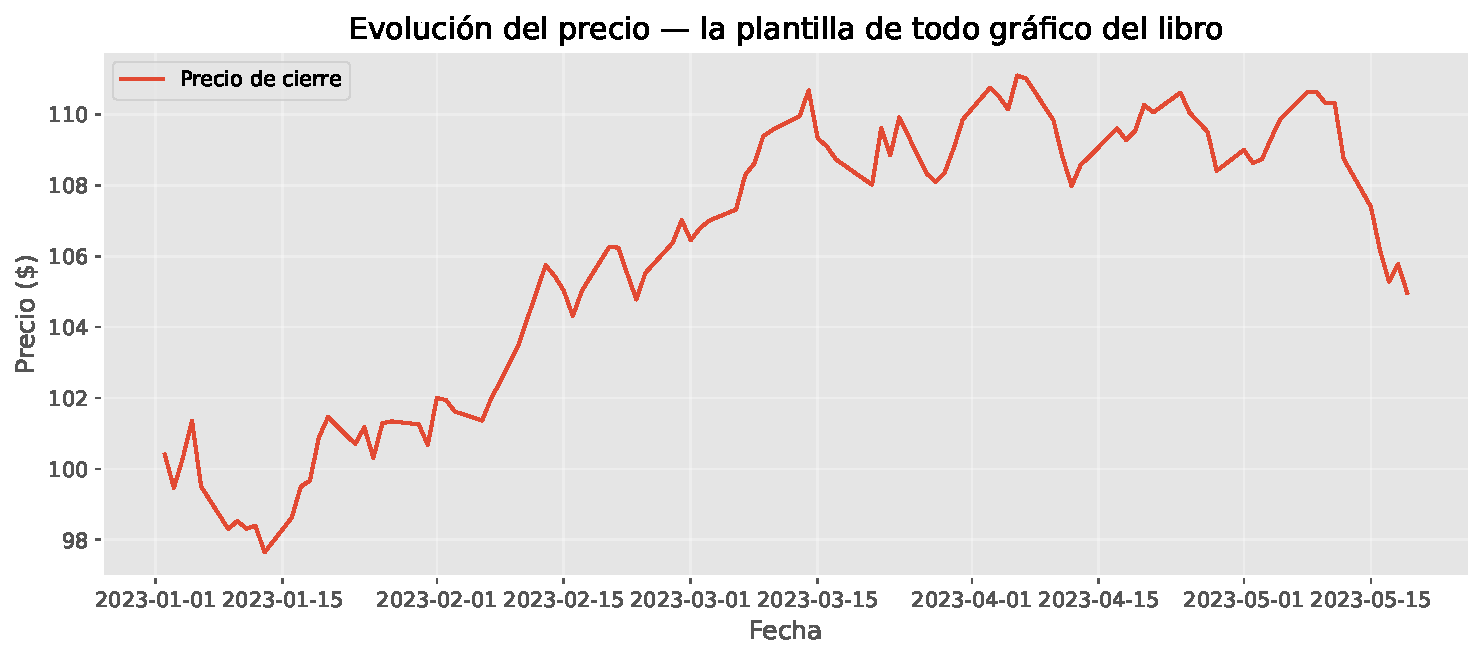
\includegraphics[keepaspectratio]{unidad1/cap06_series_tiempo_pandas_files/figure-pdf/matplotlib-anatomia-output-1.pdf}}

Esos cinco pasos ---crear, dibujar, etiquetar, leyenda/grilla,
mostrar--- son \textbf{la plantilla}. Todo lo demás son variaciones: qué
se dibuja en el paso 2 y cuántos gráficos conviven en el lienzo.

\subsection{Los tres tipos de gráfico del
libro}\label{los-tres-tipos-de-gruxe1fico-del-libro}

Con la plantilla fija, cambiar de tipo de gráfico es cambiar una línea.
Los tres que cubren el 95\% del análisis financiero:

\begin{itemize}
\tightlist
\item
  \textbf{Línea} (\texttt{ax.plot}): evolución en el tiempo --- precios,
  curvas, trayectorias.
\item
  \textbf{Histograma} (\texttt{ax.hist}): la \emph{distribución} de una
  variable --- la herramienta central para mirar retornos.
\item
  \textbf{Dispersión} (\texttt{ax.scatter}): la \emph{relación} entre
  dos variables --- ¿se mueven juntas?
\end{itemize}

\begin{Shaded}
\begin{Highlighting}[]
\NormalTok{retornos }\OperatorTok{=}\NormalTok{ df\_diario[}\StringTok{"Ret\_Simple"}\NormalTok{].dropna()}

\NormalTok{fig, axes }\OperatorTok{=}\NormalTok{ plt.subplots(}\DecValTok{1}\NormalTok{, }\DecValTok{2}\NormalTok{, figsize}\OperatorTok{=}\NormalTok{(}\DecValTok{11}\NormalTok{, }\DecValTok{4}\NormalTok{))}

\CommentTok{\# Histograma: ¿cómo se distribuyen los retornos diarios?}
\NormalTok{ax }\OperatorTok{=}\NormalTok{ axes[}\DecValTok{0}\NormalTok{]}
\NormalTok{ax.hist(retornos }\OperatorTok{*} \DecValTok{100}\NormalTok{, bins}\OperatorTok{=}\DecValTok{30}\NormalTok{, edgecolor}\OperatorTok{=}\StringTok{"white"}\NormalTok{, alpha}\OperatorTok{=}\FloatTok{0.8}\NormalTok{)}
\NormalTok{ax.set\_xlabel(}\StringTok{"Retorno diario (\%)"}\NormalTok{)}
\NormalTok{ax.set\_ylabel(}\StringTok{"Frecuencia (días)"}\NormalTok{)}
\NormalTok{ax.set\_title(}\StringTok{"Histograma: la distribución de retornos"}\NormalTok{)}
\NormalTok{ax.grid(}\VariableTok{True}\NormalTok{, alpha}\OperatorTok{=}\FloatTok{0.3}\NormalTok{)}

\CommentTok{\# Dispersión: ¿el retorno de ayer dice algo sobre el de hoy?}
\NormalTok{ax }\OperatorTok{=}\NormalTok{ axes[}\DecValTok{1}\NormalTok{]}
\NormalTok{ax.scatter(retornos.shift(}\DecValTok{1}\NormalTok{) }\OperatorTok{*} \DecValTok{100}\NormalTok{, retornos }\OperatorTok{*} \DecValTok{100}\NormalTok{, s}\OperatorTok{=}\DecValTok{15}\NormalTok{, alpha}\OperatorTok{=}\FloatTok{0.6}\NormalTok{)}
\NormalTok{ax.set\_xlabel(}\StringTok{"Retorno de ayer (\%)"}\NormalTok{)}
\NormalTok{ax.set\_ylabel(}\StringTok{"Retorno de hoy (\%)"}\NormalTok{)}
\NormalTok{ax.set\_title(}\StringTok{"Dispersión: retorno vs. retorno anterior"}\NormalTok{)}
\NormalTok{ax.grid(}\VariableTok{True}\NormalTok{, alpha}\OperatorTok{=}\FloatTok{0.3}\NormalTok{)}

\NormalTok{plt.tight\_layout()}
\NormalTok{plt.show()}
\end{Highlighting}
\end{Shaded}

\pandocbounded{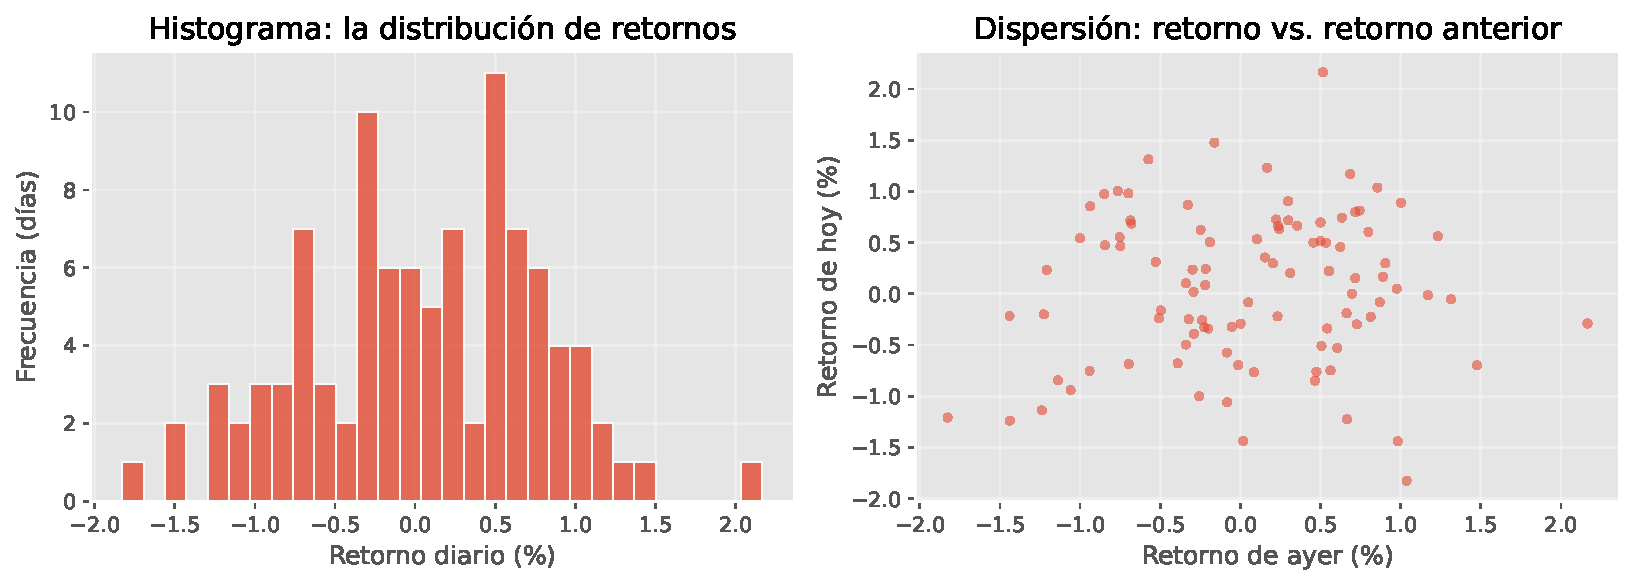
\includegraphics[keepaspectratio]{unidad1/cap06_series_tiempo_pandas_files/figure-pdf/matplotlib-tipos-output-1.pdf}}

Dos novedades en este bloque. Primero, \texttt{plt.subplots(1,\ 2)} crea
\textbf{dos gráficos en el mismo lienzo} (1 fila, 2 columnas) y devuelve
un array de Axes --- dibujás en cada uno por separado. Segundo, leé lo
que los gráficos \emph{dicen}: el histograma muestra retornos
concentrados alrededor de cero con forma de campana, y la dispersión es
una \textbf{nube sin patrón} --- el retorno de ayer no predice el de
hoy, tu primer vistazo a la eficiencia del mercado que formalizaremos en
el Capítulo 16.

\subsection{\texorpdfstring{El atajo de pandas:
\texttt{.plot()}}{El atajo de pandas: .plot()}}\label{el-atajo-de-pandas-.plot}

Pandas trae un envoltorio de matplotlib incorporado: toda Serie y
DataFrame tiene un método \texttt{.plot()} que dibuja usando \textbf{el
índice como eje x} automáticamente --- con fechas, esto es oro. Acepta
\texttt{ax=} para dirigir el dibujo a un Axes que ya creaste, así que se
combina perfecto con la plantilla:

\begin{Shaded}
\begin{Highlighting}[]
\NormalTok{fig, ax }\OperatorTok{=}\NormalTok{ plt.subplots(}\DecValTok{2}\NormalTok{, }\DecValTok{1}\NormalTok{, figsize}\OperatorTok{=}\NormalTok{(}\DecValTok{10}\NormalTok{, }\DecValTok{7}\NormalTok{), sharex}\OperatorTok{=}\VariableTok{True}\NormalTok{)}

\CommentTok{\# Panel 1: precio y su media móvil (dos series sobre el MISMO ax)}
\NormalTok{df\_diario[}\StringTok{"Precio"}\NormalTok{].plot(ax}\OperatorTok{=}\NormalTok{ax[}\DecValTok{0}\NormalTok{], label}\OperatorTok{=}\StringTok{"Precio"}\NormalTok{, alpha}\OperatorTok{=}\FloatTok{0.7}\NormalTok{)}
\NormalTok{df\_diario[}\StringTok{"SMA\_20"}\NormalTok{].plot(ax}\OperatorTok{=}\NormalTok{ax[}\DecValTok{0}\NormalTok{], label}\OperatorTok{=}\StringTok{"SMA 20"}\NormalTok{, linewidth}\OperatorTok{=}\DecValTok{2}\NormalTok{)}
\NormalTok{ax[}\DecValTok{0}\NormalTok{].set\_ylabel(}\StringTok{"Precio ($)"}\NormalTok{)}
\NormalTok{ax[}\DecValTok{0}\NormalTok{].set\_title(}\StringTok{"Precio y media móvil de 20 días"}\NormalTok{)}
\NormalTok{ax[}\DecValTok{0}\NormalTok{].legend()}
\NormalTok{ax[}\DecValTok{0}\NormalTok{].grid(}\VariableTok{True}\NormalTok{, alpha}\OperatorTok{=}\FloatTok{0.3}\NormalTok{)}

\CommentTok{\# Panel 2: la volatilidad móvil, compartiendo el eje de fechas (sharex)}
\NormalTok{(df\_diario[}\StringTok{"Vol\_20"}\NormalTok{] }\OperatorTok{*} \DecValTok{100}\NormalTok{).plot(ax}\OperatorTok{=}\NormalTok{ax[}\DecValTok{1}\NormalTok{], color}\OperatorTok{=}\StringTok{"darkorange"}\NormalTok{, label}\OperatorTok{=}\StringTok{"Volatilidad 20d"}\NormalTok{)}
\NormalTok{ax[}\DecValTok{1}\NormalTok{].set\_ylabel(}\StringTok{"Vol. anualizada (\%)"}\NormalTok{)}
\NormalTok{ax[}\DecValTok{1}\NormalTok{].set\_xlabel(}\StringTok{"Fecha"}\NormalTok{)}
\NormalTok{ax[}\DecValTok{1}\NormalTok{].set\_title(}\StringTok{"Volatilidad móvil anualizada"}\NormalTok{)}
\NormalTok{ax[}\DecValTok{1}\NormalTok{].legend()}
\NormalTok{ax[}\DecValTok{1}\NormalTok{].grid(}\VariableTok{True}\NormalTok{, alpha}\OperatorTok{=}\FloatTok{0.3}\NormalTok{)}

\NormalTok{plt.tight\_layout()}
\NormalTok{plt.show()}
\end{Highlighting}
\end{Shaded}

\pandocbounded{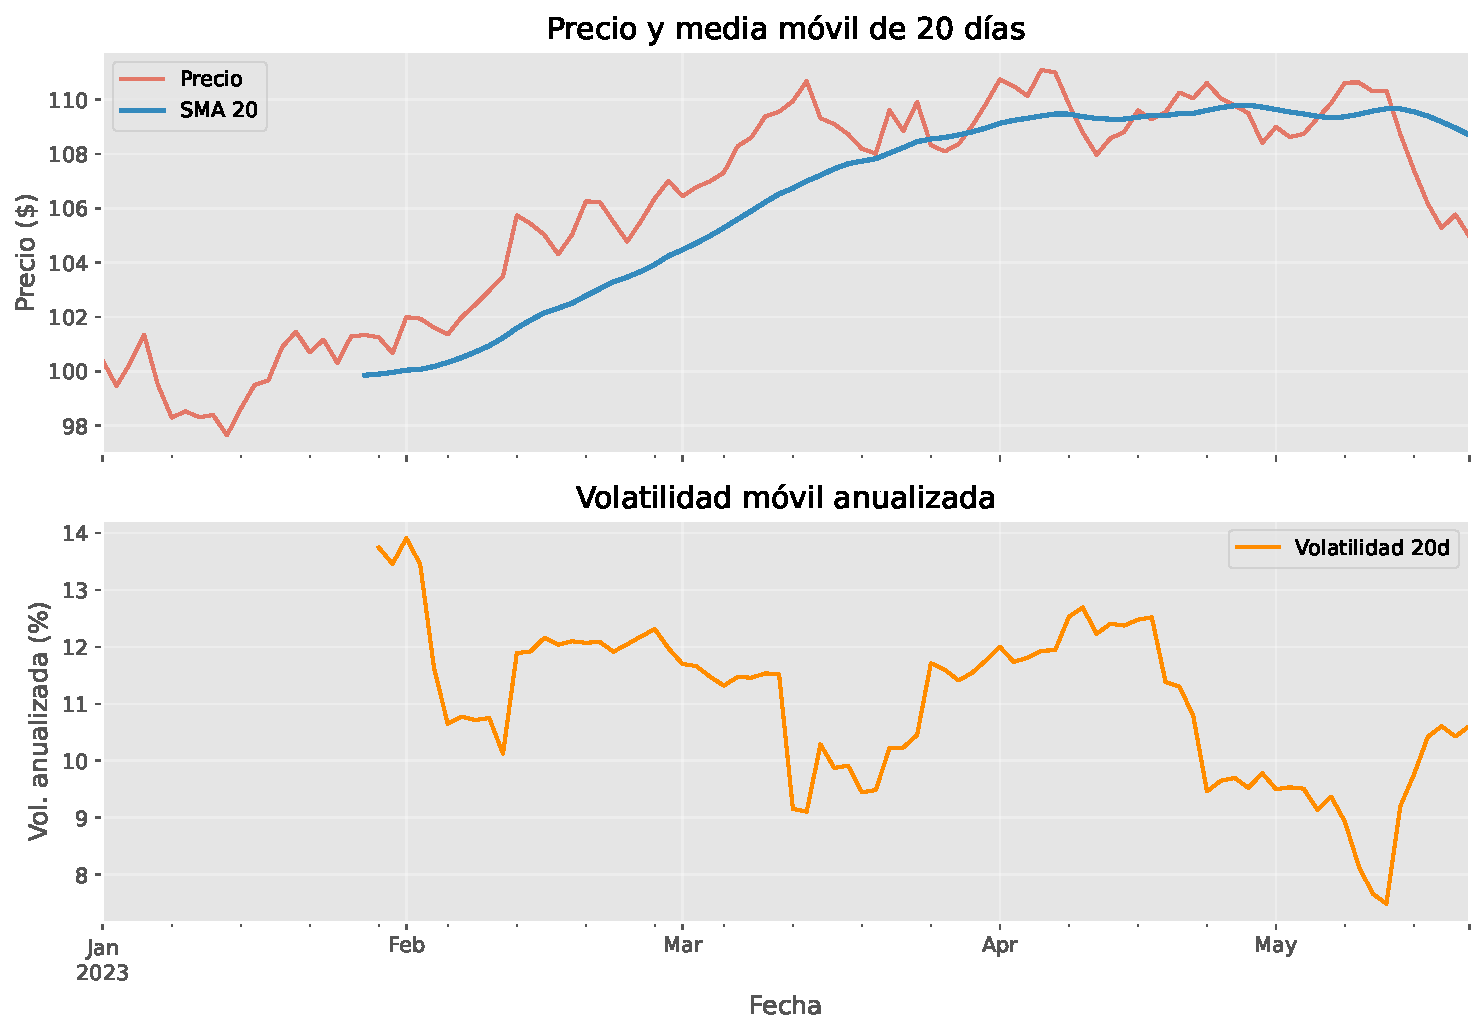
\includegraphics[keepaspectratio]{unidad1/cap06_series_tiempo_pandas_files/figure-pdf/plot-complejo-output-1.pdf}}

Este panel doble es el formato clásico del análisis técnico: precio
arriba, indicador abajo, \textbf{compartiendo el eje de fechas}
(\texttt{sharex=True}) para poder leerlos en vertical: fijate cómo los
períodos de precio ``nervioso'' en el panel superior coinciden con los
picos de volatilidad en el inferior.

\begin{tcolorbox}[enhanced jigsaw, bottomrule=.15mm, colback=white, opacitybacktitle=0.6, arc=.35mm, toprule=.15mm, opacityback=0, breakable, titlerule=0mm, left=2mm, coltitle=black, colbacktitle=quarto-callout-tip-color!10!white, colframe=quarto-callout-tip-color-frame, leftrule=.75mm, toptitle=1mm, bottomtitle=1mm, title=\textcolor{quarto-callout-tip-color}{\faLightbulb}\hspace{0.5em}{El checklist de todo gráfico}, rightrule=.15mm]

Antes de dar por terminada una figura, cuatro preguntas: ¿los
\textbf{ejes} tienen etiqueta con unidades? ¿el \textbf{título} dice qué
estoy mirando? ¿hay \textbf{leyenda} si conviven varias series? ¿alguien
que no vio el código entiende el gráfico solo? Un gráfico sin etiquetas
es un dibujo; con etiquetas, es un argumento.

\end{tcolorbox}

\begin{center}\rule{0.5\linewidth}{0.5pt}\end{center}

\section{Caso de Uso: Construcción de la Curva de
Rendimientos}\label{caso-de-uso-construcciuxf3n-de-la-curva-de-rendimientos}

Este caso integra casi todo el capítulo ---DataFrames, iteración,
operaciones vectorizadas--- para resolver un problema central de la
renta fija: \textbf{construir la curva de tasas} a partir de precios de
bonos que se cotizan en el mercado.

\subsection{¿Por qué necesitamos ``construir'' una
curva?}\label{por-quuxe9-necesitamos-construir-una-curva}

En el mercado no observamos directamente las tasas \emph{spot} (la tasa
de un instrumento que paga todo al vencimiento, sin cupones
intermedios). Lo que observamos son \textbf{precios de bonos con cupón},
y cada uno mezcla tasas de muchos plazos a la vez. La técnica del
\textbf{bootstrapping} desarma esa mezcla plazo por plazo: usa el bono a
1 año para despejar la tasa a 1 año, y con esa tasa ya conocida despeja
la de 2 años del bono a 2 años, y así sucesivamente. Es como armar la
curva ``tirando del hilo''.

La Figura~\ref{fig-bootstrapping} muestra la cadena: cada tasa que se
despeja se convierte en un insumo para el paso siguiente.

\begin{figure}

\centering{

\includegraphics[width=12.6in,height=2.48in]{unidad1/cap06_series_tiempo_pandas_files/figure-latex/mermaid-figure-2.png}

}

\caption{\label{fig-bootstrapping}Bootstrapping de la curva spot. Cada
bono, junto con las tasas ya despejadas, deja una sola incógnita: la
tasa spot de su propio plazo. Con dos spots consecutivas se obtiene la
forward implícita entre ellas.}

\end{figure}%

Para un bono a \(n\) años con cupón anual \(C\) y valor nominal \(VN\),
su precio es la suma de todos los flujos descontados a la tasa spot
correspondiente a cada plazo:

\[P = \sum_{t=1}^{n-1} \frac{C}{(1 + z_t)^t} + \frac{C + VN}{(1 + z_n)^n}\]

Si ya conocemos las tasas \(z_1, \dots, z_{n-1}\) (de los pasos
anteriores), la única incógnita es \(z_n\), y la despejamos.

\phantomsection\label{bootstrapping-final}
\begin{Shaded}
\begin{Highlighting}[]
\NormalTok{bonos\_mkt }\OperatorTok{=}\NormalTok{ pd.DataFrame([}
\NormalTok{    \{}\StringTok{"maturity"}\NormalTok{: }\DecValTok{1}\NormalTok{, }\StringTok{"cupon"}\NormalTok{: }\FloatTok{0.05}\NormalTok{, }\StringTok{"precio"}\NormalTok{: }\FloatTok{100.0}\NormalTok{\},}
\NormalTok{    \{}\StringTok{"maturity"}\NormalTok{: }\DecValTok{2}\NormalTok{, }\StringTok{"cupon"}\NormalTok{: }\FloatTok{0.06}\NormalTok{, }\StringTok{"precio"}\NormalTok{: }\FloatTok{100.5}\NormalTok{\},}
\NormalTok{    \{}\StringTok{"maturity"}\NormalTok{: }\DecValTok{3}\NormalTok{, }\StringTok{"cupon"}\NormalTok{: }\FloatTok{0.065}\NormalTok{, }\StringTok{"precio"}\NormalTok{: }\FloatTok{99.8}\NormalTok{\},}
\NormalTok{    \{}\StringTok{"maturity"}\NormalTok{: }\DecValTok{4}\NormalTok{, }\StringTok{"cupon"}\NormalTok{: }\FloatTok{0.07}\NormalTok{, }\StringTok{"precio"}\NormalTok{: }\FloatTok{100.2}\NormalTok{\},}
\NormalTok{    \{}\StringTok{"maturity"}\NormalTok{: }\DecValTok{5}\NormalTok{, }\StringTok{"cupon"}\NormalTok{: }\FloatTok{0.075}\NormalTok{, }\StringTok{"precio"}\NormalTok{: }\FloatTok{99.5}\NormalTok{\},}
\NormalTok{]).set\_index(}\StringTok{"maturity"}\NormalTok{)}

\NormalTok{tasas\_spot }\OperatorTok{=}\NormalTok{ pd.Series(index}\OperatorTok{=}\NormalTok{bonos\_mkt.index, dtype}\OperatorTok{=}\BuiltInTok{float}\NormalTok{)}
\NormalTok{VN }\OperatorTok{=} \DecValTok{100}

\ControlFlowTok{for}\NormalTok{ n, bono }\KeywordTok{in}\NormalTok{ bonos\_mkt.iterrows():}
\NormalTok{    C }\OperatorTok{=}\NormalTok{ VN }\OperatorTok{*}\NormalTok{ bono[}\StringTok{"cupon"}\NormalTok{]}
\NormalTok{    P }\OperatorTok{=}\NormalTok{ bono[}\StringTok{"precio"}\NormalTok{]}

    \CommentTok{\# Valor presente de los cupones anteriores al vencimiento,}
    \CommentTok{\# descontados con las tasas spot ya calculadas en pasos previos}
\NormalTok{    vp\_cupones }\OperatorTok{=} \BuiltInTok{sum}\NormalTok{(C }\OperatorTok{/}\NormalTok{ (}\DecValTok{1} \OperatorTok{+}\NormalTok{ tasas\_spot[t]) }\OperatorTok{**}\NormalTok{ t }\ControlFlowTok{for}\NormalTok{ t }\KeywordTok{in} \BuiltInTok{range}\NormalTok{(}\DecValTok{1}\NormalTok{, }\BuiltInTok{int}\NormalTok{(n)))}

    \CommentTok{\# Despejamos la tasa spot del plazo n del flujo final (cupón + nominal)}
\NormalTok{    z\_n }\OperatorTok{=}\NormalTok{ ((C }\OperatorTok{+}\NormalTok{ VN) }\OperatorTok{/}\NormalTok{ (P }\OperatorTok{{-}}\NormalTok{ vp\_cupones)) }\OperatorTok{**}\NormalTok{ (}\DecValTok{1} \OperatorTok{/}\NormalTok{ n) }\OperatorTok{{-}} \DecValTok{1}
\NormalTok{    tasas\_spot[n] }\OperatorTok{=}\NormalTok{ z\_n}

\BuiltInTok{print}\NormalTok{(}\StringTok{"Curva Spot (tasas cero{-}cupón):"}\NormalTok{)}
\BuiltInTok{print}\NormalTok{((tasas\_spot }\OperatorTok{*} \DecValTok{100}\NormalTok{).}\BuiltInTok{round}\NormalTok{(}\DecValTok{3}\NormalTok{).astype(}\BuiltInTok{str}\NormalTok{) }\OperatorTok{+} \StringTok{" \%"}\NormalTok{)}
\end{Highlighting}
\end{Shaded}

\begin{verbatim}
Curva Spot (tasas cero-cupón):
maturity
1      5.0 %
2     5.75 %
3    6.649 %
4    7.042 %
5    7.826 %
dtype: object
\end{verbatim}

\subsection{De la curva spot a las tasas
forward}\label{de-la-curva-spot-a-las-tasas-forward}

La curva spot responde \emph{``¿a qué tasa presto hoy por 3 años?''}.
Pero muchas veces queremos saber otra cosa: \emph{``¿qué tasa está
descontando el mercado para el año que va del 2 al 3?''}. Esa es la
\textbf{tasa forward implícita}, y sale de un argumento de no-arbitraje:
invertir 3 años a la spot \(z_3\) debe rendir lo mismo que invertir 2
años a \(z_2\) y luego reinvertir 1 año a la forward \(f_{2,3}\):

\[(1 + z_n)^n = (1 + z_{n-1})^{n-1} \cdot (1 + f_{n-1,n}) \quad\Rightarrow\quad f_{n-1,n} = \frac{(1 + z_n)^n}{(1 + z_{n-1})^{n-1}} - 1\]

\phantomsection\label{forward-rates}
\begin{Shaded}
\begin{Highlighting}[]
\CommentTok{\# Factor de capitalización acumulado hasta cada plazo: (1 + z\_n)\^{}n}
\NormalTok{factor\_acum }\OperatorTok{=}\NormalTok{ (}\DecValTok{1} \OperatorTok{+}\NormalTok{ tasas\_spot) }\OperatorTok{**}\NormalTok{ tasas\_spot.index}

\CommentTok{\# Forward de un año: cociente de factores acumulados consecutivos}
\NormalTok{forwards }\OperatorTok{=}\NormalTok{ factor\_acum }\OperatorTok{/}\NormalTok{ factor\_acum.shift(}\DecValTok{1}\NormalTok{) }\OperatorTok{{-}} \DecValTok{1}
\NormalTok{forwards.iloc[}\DecValTok{0}\NormalTok{] }\OperatorTok{=}\NormalTok{ tasas\_spot.iloc[}\DecValTok{0}\NormalTok{]  }\CommentTok{\# el forward del primer tramo es la spot a 1 año}

\NormalTok{curva }\OperatorTok{=}\NormalTok{ pd.DataFrame(\{}\StringTok{"spot"}\NormalTok{: tasas\_spot, }\StringTok{"forward\_1y"}\NormalTok{: forwards\})}
\BuiltInTok{print}\NormalTok{((curva }\OperatorTok{*} \DecValTok{100}\NormalTok{).}\BuiltInTok{round}\NormalTok{(}\DecValTok{3}\NormalTok{))}
\end{Highlighting}
\end{Shaded}

\begin{verbatim}
           spot  forward_1y
maturity                   
1         5.000       5.000
2         5.750       6.506
3         6.649       8.469
4         7.042       8.228
5         7.826      11.022
\end{verbatim}

Cuando las forward están \textbf{por encima} de las spot, el mercado
espera que las tasas suban (curva creciente): cada tramo nuevo
``empuja'' el promedio hacia arriba.

\subsection{Interpolar la curva para plazos
intermedios}\label{interpolar-la-curva-para-plazos-intermedios}

Nuestra curva tiene puntos solo en 1, 2, 3, 4 y 5 años, pero en la
práctica necesitamos descontar flujos que caen en cualquier fecha (por
ejemplo, a 2,5 años). Para eso \textbf{interpolamos}. Pandas trae
\texttt{interpolate()}, que rellena los huecos de un índice: reindexamos
la curva a una grilla más fina y dejamos que complete linealmente.

\begin{Shaded}
\begin{Highlighting}[]
\CommentTok{\# Grilla de plazos cada medio año, de 1 a 5}
\NormalTok{grilla }\OperatorTok{=}\NormalTok{ np.arange(}\FloatTok{1.0}\NormalTok{, }\FloatTok{5.5}\NormalTok{, }\FloatTok{0.5}\NormalTok{)}

\NormalTok{curva\_interpolada }\OperatorTok{=}\NormalTok{ (}
\NormalTok{    tasas\_spot}
\NormalTok{    .reindex(tasas\_spot.index.union(grilla))  }\CommentTok{\# agregamos los plazos intermedios (quedan NaN)}
\NormalTok{    .interpolate(method}\OperatorTok{=}\StringTok{"index"}\NormalTok{)              }\CommentTok{\# interpolamos usando el valor del índice (el plazo)}
\NormalTok{    .reindex(grilla)                           }\CommentTok{\# nos quedamos con la grilla fina}
\NormalTok{)}

\NormalTok{fig, ax }\OperatorTok{=}\NormalTok{ plt.subplots(figsize}\OperatorTok{=}\NormalTok{(}\DecValTok{9}\NormalTok{, }\DecValTok{4}\NormalTok{))}
\NormalTok{ax.plot(tasas\_spot.index, tasas\_spot }\OperatorTok{*} \DecValTok{100}\NormalTok{, }\StringTok{"o"}\NormalTok{, markersize}\OperatorTok{=}\DecValTok{9}\NormalTok{,}
\NormalTok{        label}\OperatorTok{=}\StringTok{"Tasas spot observadas (bootstrapping)"}\NormalTok{)}
\NormalTok{ax.plot(curva\_interpolada.index, curva\_interpolada }\OperatorTok{*} \DecValTok{100}\NormalTok{, }\StringTok{".{-}"}\NormalTok{, alpha}\OperatorTok{=}\FloatTok{0.7}\NormalTok{,}
\NormalTok{        label}\OperatorTok{=}\StringTok{"Curva interpolada (cada 6 meses)"}\NormalTok{)}
\NormalTok{ax.set\_xlabel(}\StringTok{"Plazo (años)"}\NormalTok{)}
\NormalTok{ax.set\_ylabel(}\StringTok{"Tasa spot (\%)"}\NormalTok{)}
\NormalTok{ax.set\_title(}\StringTok{"Curva de Rendimientos: puntos observados vs. interpolación"}\NormalTok{)}
\NormalTok{ax.legend()}
\NormalTok{ax.grid(}\VariableTok{True}\NormalTok{, alpha}\OperatorTok{=}\FloatTok{0.3}\NormalTok{)}
\NormalTok{plt.tight\_layout()}
\NormalTok{plt.show()}
\end{Highlighting}
\end{Shaded}

\pandocbounded{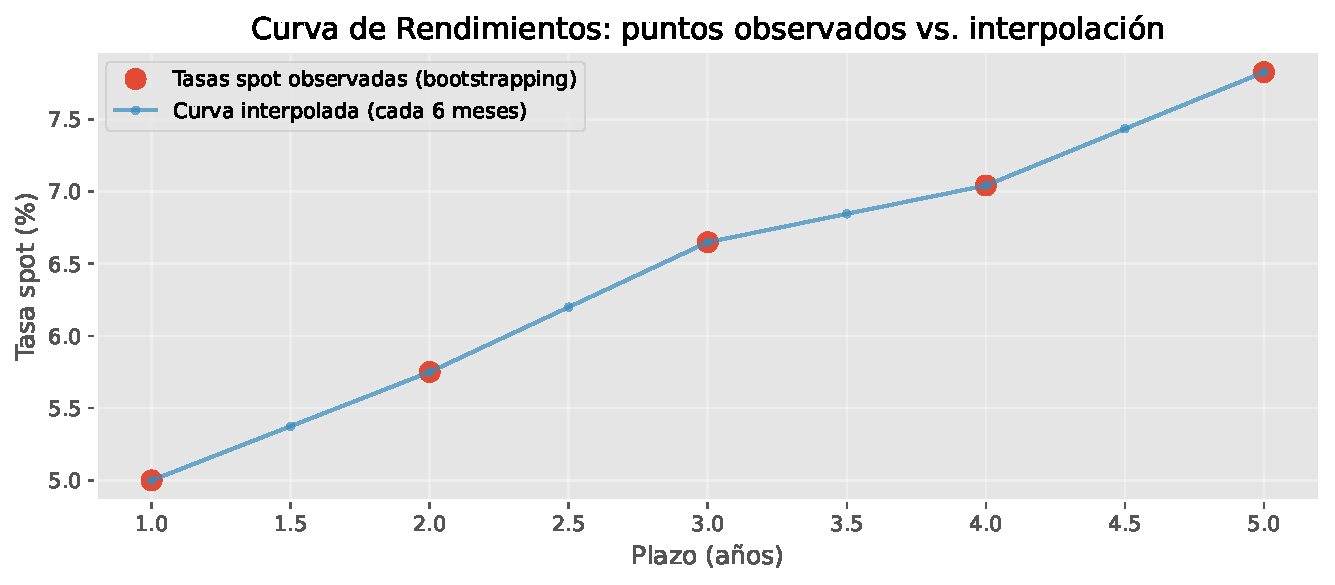
\includegraphics[keepaspectratio]{unidad1/cap06_series_tiempo_pandas_files/figure-pdf/interpolacion-curva-output-1.pdf}}

\begin{tcolorbox}[enhanced jigsaw, bottomrule=.15mm, colback=white, opacitybacktitle=0.6, arc=.35mm, toprule=.15mm, opacityback=0, breakable, titlerule=0mm, left=2mm, coltitle=black, colbacktitle=quarto-callout-warning-color!10!white, colframe=quarto-callout-warning-color-frame, leftrule=.75mm, toptitle=1mm, bottomtitle=1mm, title=\textcolor{quarto-callout-warning-color}{\faExclamationTriangle}\hspace{0.5em}{La interpolación lineal es un punto de partida, no la verdad}, rightrule=.15mm]

Interpolar linealmente es simple y transparente, pero los operadores de
renta fija suelen usar métodos más suaves (splines cúbicos,
Nelson-Siegel) para que la curva forward no tenga ``quiebres''
antieconómicos. Para aprender el mecanismo, lo lineal alcanza; para
valuar en producción, conviene ir más fino.

\end{tcolorbox}

\begin{center}\rule{0.5\linewidth}{0.5pt}\end{center}

\section{Errores comunes}\label{errores-comunes-4}

\begin{tcolorbox}[enhanced jigsaw, bottomrule=.15mm, colback=white, opacitybacktitle=0.6, arc=.35mm, toprule=.15mm, opacityback=0, breakable, titlerule=0mm, left=2mm, coltitle=black, colbacktitle=quarto-callout-warning-color!10!white, colframe=quarto-callout-warning-color-frame, leftrule=.75mm, toptitle=1mm, bottomtitle=1mm, title=\textcolor{quarto-callout-warning-color}{\faExclamationTriangle}\hspace{0.5em}{Trampas frecuentes}, rightrule=.15mm]

\begin{itemize}
\tightlist
\item
  \textbf{Fechas como texto}: si olvidás \texttt{parse\_dates} (o
  \texttt{pd.to\_datetime}), las fechas quedan como strings: se ordenan
  alfabéticamente, \texttt{resample} falla y los gráficos salen
  desordenados. Verificá con \texttt{df.index.dtype}.
\item
  \textbf{El \texttt{NaN} inicial de \texttt{pct\_change()}}: la primera
  observación de cualquier serie de retornos es \texttt{NaN}. Si después
  calculás \texttt{mean()} no pasa nada (pandas lo ignora), pero si
  convertís a NumPy o lo pasás a otra librería, ese \texttt{NaN} propaga
  y arruina el cálculo. \texttt{dropna()} primero.
\item
  \textbf{\texttt{ffill} con huecos largos}: arrastrar un precio un día
  es razonable; arrastrarlo tres meses (un bono que dejó de cotizar)
  fabrica una serie plana con volatilidad cero --- un activo ``sin
  riesgo'' que no existe. Poné un límite (\texttt{ffill(limit=5)}) o
  revisá los huecos antes.
\item
  \textbf{Look-ahead con \texttt{shift} al revés}: \texttt{shift(-1)}
  trae el dato de \emph{mañana} a la fila de hoy. Útil para armar
  targets de predicción, letal si se te cuela en una señal de trading:
  estarías operando con información del futuro (el tema central del
  Capítulo 17).
\item
  \textbf{\texttt{SettingWithCopyWarning}}: asignar sobre un ``recorte''
  de un DataFrame
  (\texttt{df{[}df.x\ \textgreater{}\ 0{]}{[}"y"{]}\ =\ 1}) puede
  modificar una copia y no el original. La forma segura es una sola
  indexación con \texttt{.loc}:
  \texttt{df.loc{[}df.x\ \textgreater{}\ 0,\ "y"{]}\ =\ 1}.
\end{itemize}

\end{tcolorbox}

\begin{center}\rule{0.5\linewidth}{0.5pt}\end{center}

\section{Ejercicios Propuestos}\label{ejercicios-propuestos-5}

\begin{tcolorbox}[enhanced jigsaw, bottomrule=.15mm, colback=white, opacitybacktitle=0.6, arc=.35mm, toprule=.15mm, opacityback=0, breakable, titlerule=0mm, left=2mm, coltitle=black, colbacktitle=quarto-callout-important-color!10!white, colframe=quarto-callout-important-color-frame, leftrule=.75mm, toptitle=1mm, bottomtitle=1mm, title=\textcolor{quarto-callout-important-color}{\faExclamation}\hspace{0.5em}{Desafíos}, rightrule=.15mm]

\begin{enumerate}
\def\labelenumi{\arabic{enumi}.}
\tightlist
\item
  \textbf{Volatilidad comparada}: A partir de una serie de precios
  simulada, compará la volatilidad móvil de 30 días contra la de 90 días
  en un mismo gráfico. ¿Cuál reacciona más rápido a un shock?
\item
  \textbf{Dashboard de retornos}: Escribí una función que reciba un
  DataFrame de precios y devuelva una tabla resumen con retorno
  acumulado, volatilidad anualizada y máximo \emph{drawdown}.
\item
  \textbf{Groupby + resample}: Dado un panel de varios activos, calculá
  el retorno promedio mensual de cada uno combinando \texttt{.groupby()}
  con \texttt{.resample()}.
\item
  \textbf{\texttt{ffill} vs.~\texttt{interpolate}}: Simulá una serie con
  valores nulos aleatorios y compará el resultado de rellenarlos con
  \texttt{ffill()} frente a \texttt{interpolate()}. ¿Cuándo es apropiado
  cada uno?
\item
  \textbf{Curva forward completa}: Extendé el ejemplo de bootstrapping
  para calcular, además de las forward de 1 año, la tasa forward a 2
  años que arranca dentro de 1 año (\(f_{1,3}\)).
\end{enumerate}

\end{tcolorbox}

\begin{center}\rule{0.5\linewidth}{0.5pt}\end{center}

\section{Referencias}\label{referencias-5}

\phantomsection\label{refs}

\part{Módulo 2: Teoría de Portafolios y Optimización}

\chapter*{Módulo 2: Teoría de Portafolios y
Optimización}\label{muxf3dulo-2-teoruxeda-de-portafolios-y-optimizaciuxf3n-1}
\addcontentsline{toc}{chapter}{Módulo 2: Teoría de Portafolios y
Optimización}

\markboth{Módulo 2: Teoría de Portafolios y Optimización}{Módulo 2:
Teoría de Portafolios y Optimización}

\emph{De describir activos a decidir entre ellos}

En el Módulo 1 aprendiste a analizar instrumentos \textbf{de a uno}:
valuar un bono, calcular el retorno de una acción, graficar su historia.
Pero ningún inversor real tiene un solo activo, y la pregunta que de
verdad importa es otra: \textbf{¿cómo reparto mi capital entre todos los
activos disponibles?} Este módulo construye la respuesta cuantitativa a
esa pregunta --- y también sus contraejemplos.

El recorrido tiene forma de tesis, antítesis y síntesis. Primero armamos
las herramientas: \textbf{estadística de retornos} (¿cómo se comporta
cada activo?) y \textbf{optimización numérica} (¿cómo le pido a la
computadora que encuentre ``lo mejor''?). Con eso construimos el
edificio clásico: la \textbf{frontera eficiente de Markowitz}, la idea
ganadora del Nobel de que la diversificación se puede medir y optimizar.
Hasta ahí la teoría es hermosa.

Después viene la parte que los libros suelen esquivar: \textbf{en la
práctica, Markowitz falla}. Es hipersensible a estimaciones que son puro
ruido, y produce carteras extremas que ningún gestor firmaría. Los
últimos dos capítulos presentan las dos respuestas modernas más
importantes a ese problema, que atacan por flancos opuestos:
\textbf{HRP} (López de Prado, 2016) esquiva la matemática frágil usando
clustering jerárquico, y \textbf{Black-Litterman} (Goldman Sachs, 1992)
disciplina las estimaciones partiendo del equilibrio del mercado y
mezclándolo con tus opiniones según tu confianza. Al final del módulo no
solo vas a saber optimizar un portafolio: vas a saber \textbf{cuándo
desconfiar del optimizador} --- que es la habilidad que separa al que
aprendió la fórmula del que entiende el problema.

\begin{tcolorbox}[enhanced jigsaw, bottomrule=.15mm, colback=white, breakable, left=2mm, colframe=quarto-callout-note-color-frame, leftrule=.75mm, arc=.35mm, toprule=.15mm, rightrule=.15mm, opacityback=0]
\begin{minipage}[t]{5.5mm}
\textcolor{quarto-callout-note-color}{\faInfo}
\end{minipage}%
\begin{minipage}[t]{\textwidth - 5.5mm}

\vspace{-3mm}\textbf{Lo que este módulo asume}\vspace{3mm}

Usamos intensivamente el álgebra matricial de NumPy (Capítulo 5) --- en
particular \texttt{@}, \texttt{np.linalg} y la matriz de covarianzas ---
y la estadística descriptiva del Capítulo 6. Si esos temas no te
quedaron firmes, vale la pena repasarlos antes de entrar a Markowitz.

\end{minipage}%
\end{tcolorbox}

\begin{center}\rule{0.5\linewidth}{0.5pt}\end{center}

\section*{🎯 Objetivos de Aprendizaje}\label{objetivos-de-aprendizaje-1}
\addcontentsline{toc}{section}{🎯 Objetivos de Aprendizaje}

\markright{🎯 Objetivos de Aprendizaje}

Al completar este módulo, vas a ser capaz de:

\begin{enumerate}
\def\labelenumi{\arabic{enumi}.}
\tightlist
\item
  \textbf{Analizar distribuciones} de retornos con estadística
  descriptiva y tests de normalidad.
\item
  \textbf{Construir la frontera eficiente} de Markowitz y encontrar el
  portafolio tangente (máximo Sharpe).
\item
  \textbf{Elegir la métrica correcta} (Sharpe, Sortino, mínima varianza)
  según el objetivo del inversor.
\item
  \textbf{Aplicar Hierarchical Risk Parity} para sortear la
  inestabilidad de la optimización clásica.
\item
  \textbf{Incorporar tus views} al equilibrio del mercado con el modelo
  de Black-Litterman.
\end{enumerate}

\begin{center}\rule{0.5\linewidth}{0.5pt}\end{center}

\section*{🗓️ Recorrido Capítulo a
Capítulo}\label{recorrido-capuxedtulo-a-capuxedtulo-1}
\addcontentsline{toc}{section}{🗓️ Recorrido Capítulo a Capítulo}

\markright{🗓️ Recorrido Capítulo a Capítulo}

\begin{longtable}[]{@{}
  >{\centering\arraybackslash}p{(\linewidth - 6\tabcolsep) * \real{0.2500}}
  >{\raggedright\arraybackslash}p{(\linewidth - 6\tabcolsep) * \real{0.1875}}
  >{\raggedright\arraybackslash}p{(\linewidth - 6\tabcolsep) * \real{0.2500}}
  >{\raggedright\arraybackslash}p{(\linewidth - 6\tabcolsep) * \real{0.3125}}@{}}
\toprule\noalign{}
\begin{minipage}[b]{\linewidth}\centering
Capítulo
\end{minipage} & \begin{minipage}[b]{\linewidth}\raggedright
Tema
\end{minipage} & \begin{minipage}[b]{\linewidth}\raggedright
Python
\end{minipage} & \begin{minipage}[b]{\linewidth}\raggedright
Finanzas
\end{minipage} \\
\midrule\noalign{}
\endhead
\bottomrule\noalign{}
\endlastfoot
\textbf{7} & Estadística y Optimización & \texttt{scipy.stats},
\texttt{scipy.optimize}, histogramas & Media, varianza, curtosis,
normalidad \\
\textbf{8} & Markowitz y Frontera Eficiente & \texttt{numpy} matricial,
\texttt{minimize()} & Σ, Sharpe, Sortino, CML, dividendos, renta fija \\
\textbf{9} & Hierarchical Risk Parity & \texttt{scipy.cluster.hierarchy}
& Clustering, riesgo, robustez fuera de muestra \\
\textbf{10} & Black-Litterman & Álgebra matricial, \texttt{np.linalg} &
Equilibrio de mercado, views, fórmula maestra \\
\end{longtable}

\begin{center}\rule{0.5\linewidth}{0.5pt}\end{center}

\section*{🧰 Herramientas y
Librerías}\label{herramientas-y-libreruxedas-1}
\addcontentsline{toc}{section}{🧰 Herramientas y Librerías}

\markright{🧰 Herramientas y Librerías}

\textbf{NumPy}

Álgebra matricial

\textbf{SciPy}

Optimización, estadística y clustering

\textbf{Matplotlib}

Frontera eficiente y dendrogramas

\begin{center}\rule{0.5\linewidth}{0.5pt}\end{center}

\section*{🔑 Concepto Clave:
Media-Varianza}\label{concepto-clave-media-varianza}
\addcontentsline{toc}{section}{🔑 Concepto Clave: Media-Varianza}

\markright{🔑 Concepto Clave: Media-Varianza}

\begin{tcolorbox}[enhanced jigsaw, bottomrule=.15mm, colback=white, breakable, left=2mm, colframe=quarto-callout-important-color-frame, leftrule=.75mm, arc=.35mm, toprule=.15mm, rightrule=.15mm, opacityback=0]
\begin{minipage}[t]{5.5mm}
\textcolor{quarto-callout-important-color}{\faExclamation}
\end{minipage}%
\begin{minipage}[t]{\textwidth - 5.5mm}

El framework de Markowitz plantea que un inversor racional elige
portafolios que \textbf{maximizan retorno} para un nivel dado de riesgo,
o equivalentemente, \textbf{minimizan riesgo} para un retorno objetivo.
La solución al problema de optimización genera la \textbf{frontera
eficiente}.

\[\min_{\mathbf{w}} \quad \mathbf{w}^T \boldsymbol{\Sigma} \mathbf{w} \quad \text{sujeto a} \quad \mathbf{w}^T \boldsymbol{\mu} = \mu^*, \quad \mathbf{w}^T \mathbf{1} = 1\]

El resto del módulo puede leerse como una conversación con esta fórmula:
cómo resolverla, qué esconde y cómo arreglarla.

\end{minipage}%
\end{tcolorbox}

\begin{center}\rule{0.5\linewidth}{0.5pt}\end{center}

\section*{📚 Lecturas Recomendadas}\label{lecturas-recomendadas-1}
\addcontentsline{toc}{section}{📚 Lecturas Recomendadas}

\markright{📚 Lecturas Recomendadas}

\begin{itemize}
\tightlist
\item
  Markowitz, H. (1952). \emph{Portfolio Selection}. The Journal of
  Finance.
\item
  Elton, E. et al.~(2014). \emph{Modern Portfolio Theory and Investment
  Analysis}. Wiley.
\item
  Black, F., \& Litterman, R. (1992). \emph{Global Portfolio
  Optimization}. Financial Analysts Journal.
\item
  López de Prado, M. (2016). \emph{Building Diversified Portfolios that
  Outperform Out of Sample}. The Journal of Portfolio Management.
\end{itemize}

\chapter{Capítulo 7: Estadística Descriptiva y Optimización
Matemática}\label{capuxedtulo-7-estaduxedstica-descriptiva-y-optimizaciuxf3n-matemuxe1tica}

Distribuciones de retornos, scipy.stats y scipy.optimize

Antes de armar portafolios necesitamos dos herramientas: saber describir
estadísticamente cómo se comportan los retornos (media, volatilidad,
asimetría, curtosis, y el test de si son ``normales'') y saber pedirle a
la computadora que encuentre el mejor valor de algo (optimización
numérica con scipy). Este capítulo construye ambas, que se combinan en
el capítulo siguiente con Markowitz.

\hfill\break

\chapter{Introducción}\label{introducciuxf3n-6}

Este módulo trata de una pregunta: \emph{¿cómo repartir el capital entre
activos?} Para responderla con rigor necesitamos dos habilidades
previas.

La primera es \textbf{describir el comportamiento de los retornos}. ``La
acción rinde 10\% anual'' es una descripción pobre: ¿con cuánta
variabilidad? ¿las sorpresas son simétricas o hay derrumbes ocasionales?
¿los extremos son raros o frecuentes? La estadística descriptiva pone
números a esas preguntas.

La segunda es \textbf{optimizar}: dado un objetivo (``minimizar el
riesgo'', ``maximizar la utilidad'') y restricciones (``los pesos suman
1'', ``sin ventas en corto''), encontrar la mejor solución. Si venís del
mundo Excel, esto es lo que hacía el \emph{Solver} --- pero programable,
más rápido y reproducible.

\phantomsection\label{setup}
\begin{Shaded}
\begin{Highlighting}[]
\ImportTok{import}\NormalTok{ numpy }\ImportTok{as}\NormalTok{ np}
\ImportTok{import}\NormalTok{ pandas }\ImportTok{as}\NormalTok{ pd}
\ImportTok{import}\NormalTok{ matplotlib.pyplot }\ImportTok{as}\NormalTok{ plt}
\ImportTok{from}\NormalTok{ scipy }\ImportTok{import}\NormalTok{ stats}

\NormalTok{rng }\OperatorTok{=}\NormalTok{ np.random.default\_rng(}\DecValTok{42}\NormalTok{)}
\end{Highlighting}
\end{Shaded}

\begin{center}\rule{0.5\linewidth}{0.5pt}\end{center}

\chapter{Estadística descriptiva de
retornos}\label{estaduxedstica-descriptiva-de-retornos}

\section{Los cuatro momentos}\label{los-cuatro-momentos}

Una distribución de retornos se resume, en primera aproximación, con
cuatro números --- los \textbf{momentos}:

\begin{enumerate}
\def\labelenumi{\arabic{enumi}.}
\tightlist
\item
  \textbf{Media} (\(\mu\)): el retorno ``típico''. El centro de gravedad
  de la distribución.
\item
  \textbf{Varianza / volatilidad} (\(\sigma\)): cuánto se dispersan los
  retornos alrededor de la media. Es la medida clásica de riesgo.
\item
  \textbf{Asimetría} (\emph{skewness}): ¿la distribución se estira más
  hacia un lado? Skewness \textbf{negativa} = derrumbes ocasionales más
  grandes que las subas (típico de acciones); \textbf{positiva} =
  sorpresas buenas más grandes (típico de estrategias tipo lotería).
\item
  \textbf{Curtosis} (\emph{kurtosis}): ¿cuánta masa hay en las
  \textbf{colas}? Curtosis en exceso positiva significa que los eventos
  extremos son \textbf{más frecuentes} que bajo una distribución normal.
  En finanzas, casi siempre lo son.
\end{enumerate}

\phantomsection\label{estadistica}
\begin{Shaded}
\begin{Highlighting}[]
\CommentTok{\# Simulamos un año de retornos diarios de una acción}
\NormalTok{n\_dias }\OperatorTok{=} \DecValTok{252}
\NormalTok{retornos }\OperatorTok{=}\NormalTok{ rng.normal(}\FloatTok{0.0004}\NormalTok{, }\FloatTok{0.018}\NormalTok{, n\_dias)}

\BuiltInTok{print}\NormalTok{(}\StringTok{"Estadísticas descriptivas de los retornos:"}\NormalTok{)}
\BuiltInTok{print}\NormalTok{(}\SpecialStringTok{f"  Media diaria:       }\SpecialCharTok{\{}\NormalTok{np}\SpecialCharTok{.}\NormalTok{mean(retornos)}\SpecialCharTok{:.6f\}}\SpecialStringTok{"}\NormalTok{)}
\BuiltInTok{print}\NormalTok{(}\SpecialStringTok{f"  Media anualizada:   }\SpecialCharTok{\{}\NormalTok{np}\SpecialCharTok{.}\NormalTok{mean(retornos) }\OperatorTok{*} \DecValTok{252}\SpecialCharTok{:.2\%\}}\SpecialStringTok{"}\NormalTok{)}
\BuiltInTok{print}\NormalTok{(}\SpecialStringTok{f"  Volatilidad diaria: }\SpecialCharTok{\{}\NormalTok{np}\SpecialCharTok{.}\NormalTok{std(retornos)}\SpecialCharTok{:.6f\}}\SpecialStringTok{"}\NormalTok{)}
\BuiltInTok{print}\NormalTok{(}\SpecialStringTok{f"  Vol. anualizada:    }\SpecialCharTok{\{}\NormalTok{np}\SpecialCharTok{.}\NormalTok{std(retornos) }\OperatorTok{*}\NormalTok{ np}\SpecialCharTok{.}\NormalTok{sqrt(}\DecValTok{252}\NormalTok{)}\SpecialCharTok{:.2\%\}}\SpecialStringTok{"}\NormalTok{)}
\BuiltInTok{print}\NormalTok{(}\SpecialStringTok{f"  Asimetría:          }\SpecialCharTok{\{}\NormalTok{stats}\SpecialCharTok{.}\NormalTok{skew(retornos)}\SpecialCharTok{:.4f\}}\SpecialStringTok{"}\NormalTok{)}
\BuiltInTok{print}\NormalTok{(}\SpecialStringTok{f"  Curtosis (exceso):  }\SpecialCharTok{\{}\NormalTok{stats}\SpecialCharTok{.}\NormalTok{kurtosis(retornos)}\SpecialCharTok{:.4f\}}\SpecialStringTok{"}\NormalTok{)}
\end{Highlighting}
\end{Shaded}

\begin{verbatim}
Estadísticas descriptivas de los retornos:
  Media diaria:       -0.000471
  Media anualizada:   -11.86%
  Volatilidad diaria: 0.016844
  Vol. anualizada:    26.74%
  Asimetría:          0.3848
  Curtosis (exceso):  0.1543
\end{verbatim}

\begin{tcolorbox}[enhanced jigsaw, bottomrule=.15mm, colback=white, opacitybacktitle=0.6, arc=.35mm, toprule=.15mm, opacityback=0, breakable, titlerule=0mm, left=2mm, coltitle=black, colbacktitle=quarto-callout-note-color!10!white, colframe=quarto-callout-note-color-frame, leftrule=.75mm, toptitle=1mm, bottomtitle=1mm, title=\textcolor{quarto-callout-note-color}{\faInfo}\hspace{0.5em}{¿Por qué ×252 y ×√252?}, rightrule=.15mm]

Hay \textasciitilde252 ruedas bursátiles por año. Las \textbf{medias se
suman} en el tiempo (252 días de retorno medio diario), pero las
\textbf{varianzas} son las que se suman ---no los desvíos---, así que la
volatilidad escala con la \textbf{raíz} del tiempo:
\(\sigma_{anual} = \sigma_{diaria}\sqrt{252}\). Confundir estas dos
reglas es el error de anualización más común.

\end{tcolorbox}

Como simulamos con \texttt{rng.normal}, la asimetría y la curtosis dan
cerca de cero. Con retornos reales de acciones el panorama es otro:
asimetría negativa y curtosis bien positiva. Veámoslo generando retornos
más realistas, con ``sustos'' ocasionales:

\phantomsection\label{retornos-realistas}
\begin{Shaded}
\begin{Highlighting}[]
\CommentTok{\# Mezcla: 95\% días normales + 5\% días de crisis (más volátiles y sesgados a la baja)}
\NormalTok{normales }\OperatorTok{=}\NormalTok{ rng.normal(}\FloatTok{0.0008}\NormalTok{, }\FloatTok{0.012}\NormalTok{, n\_dias)}
\NormalTok{crisis }\OperatorTok{=}\NormalTok{ rng.normal(}\OperatorTok{{-}}\FloatTok{0.02}\NormalTok{, }\FloatTok{0.04}\NormalTok{, n\_dias)}
\NormalTok{es\_crisis }\OperatorTok{=}\NormalTok{ rng.random(n\_dias) }\OperatorTok{\textless{}} \FloatTok{0.05}
\NormalTok{ret\_real }\OperatorTok{=}\NormalTok{ np.where(es\_crisis, crisis, normales)}

\BuiltInTok{print}\NormalTok{(}\SpecialStringTok{f"}\SpecialCharTok{\{}\StringTok{\textquotesingle{}\textquotesingle{}}\SpecialCharTok{:22\}\{}\StringTok{\textquotesingle{}Simulado normal\textquotesingle{}}\SpecialCharTok{:\textgreater{}16\}\{}\StringTok{\textquotesingle{}Con crisis\textquotesingle{}}\SpecialCharTok{:\textgreater{}12\}}\SpecialStringTok{"}\NormalTok{)}
\BuiltInTok{print}\NormalTok{(}\SpecialStringTok{f"}\SpecialCharTok{\{}\StringTok{\textquotesingle{}Asimetría\textquotesingle{}}\SpecialCharTok{:\textless{}22\}\{}\NormalTok{stats}\SpecialCharTok{.}\NormalTok{skew(retornos)}\SpecialCharTok{:\textgreater{}16.3f\}\{}\NormalTok{stats}\SpecialCharTok{.}\NormalTok{skew(ret\_real)}\SpecialCharTok{:\textgreater{}12.3f\}}\SpecialStringTok{"}\NormalTok{)}
\BuiltInTok{print}\NormalTok{(}\SpecialStringTok{f"}\SpecialCharTok{\{}\StringTok{\textquotesingle{}Curtosis (exceso)\textquotesingle{}}\SpecialCharTok{:\textless{}22\}\{}\NormalTok{stats}\SpecialCharTok{.}\NormalTok{kurtosis(retornos)}\SpecialCharTok{:\textgreater{}16.3f\}\{}\NormalTok{stats}\SpecialCharTok{.}\NormalTok{kurtosis(ret\_real)}\SpecialCharTok{:\textgreater{}12.3f\}}\SpecialStringTok{"}\NormalTok{)}
\end{Highlighting}
\end{Shaded}

\begin{verbatim}
                       Simulado normal  Con crisis
Asimetría                        0.385      -0.894
Curtosis (exceso)                0.154       3.804
\end{verbatim}

\section{Visualizar la
distribución}\label{visualizar-la-distribuciuxf3n}

El histograma con la normal teórica superpuesta es el gráfico de
diagnóstico básico: muestra de un vistazo si las colas y la asimetría se
apartan del modelo normal.

\begin{Shaded}
\begin{Highlighting}[]
\NormalTok{fig, axes }\OperatorTok{=}\NormalTok{ plt.subplots(}\DecValTok{1}\NormalTok{, }\DecValTok{2}\NormalTok{, figsize}\OperatorTok{=}\NormalTok{(}\DecValTok{11}\NormalTok{, }\DecValTok{4}\NormalTok{), sharey}\OperatorTok{=}\VariableTok{True}\NormalTok{)}

\ControlFlowTok{for}\NormalTok{ ax, datos, titulo }\KeywordTok{in}\NormalTok{ [(axes[}\DecValTok{0}\NormalTok{], retornos, }\StringTok{"Retornos \textasciitilde{}normales"}\NormalTok{),}
\NormalTok{                          (axes[}\DecValTok{1}\NormalTok{], ret\_real, }\StringTok{"Retornos con días de crisis"}\NormalTok{)]:}
\NormalTok{    ax.hist(datos, bins}\OperatorTok{=}\DecValTok{40}\NormalTok{, density}\OperatorTok{=}\VariableTok{True}\NormalTok{, alpha}\OperatorTok{=}\FloatTok{0.7}\NormalTok{,}
\NormalTok{            color}\OperatorTok{=}\StringTok{"steelblue"}\NormalTok{, edgecolor}\OperatorTok{=}\StringTok{"white"}\NormalTok{)}
\NormalTok{    x }\OperatorTok{=}\NormalTok{ np.linspace(datos.}\BuiltInTok{min}\NormalTok{(), datos.}\BuiltInTok{max}\NormalTok{(), }\DecValTok{200}\NormalTok{)}
\NormalTok{    ax.plot(x, stats.norm.pdf(x, datos.mean(), datos.std()),}
            \StringTok{"r{-}"}\NormalTok{, linewidth}\OperatorTok{=}\DecValTok{2}\NormalTok{, label}\OperatorTok{=}\StringTok{"Normal teórica"}\NormalTok{)}
\NormalTok{    ax.set\_title(titulo)}
\NormalTok{    ax.set\_xlabel(}\StringTok{"Retorno diario"}\NormalTok{)}
\NormalTok{    ax.legend()}
\NormalTok{    ax.grid(}\VariableTok{True}\NormalTok{, alpha}\OperatorTok{=}\FloatTok{0.3}\NormalTok{)}

\NormalTok{axes[}\DecValTok{0}\NormalTok{].set\_ylabel(}\StringTok{"Densidad"}\NormalTok{)}
\NormalTok{plt.tight\_layout()}
\NormalTok{plt.show()}
\end{Highlighting}
\end{Shaded}

\pandocbounded{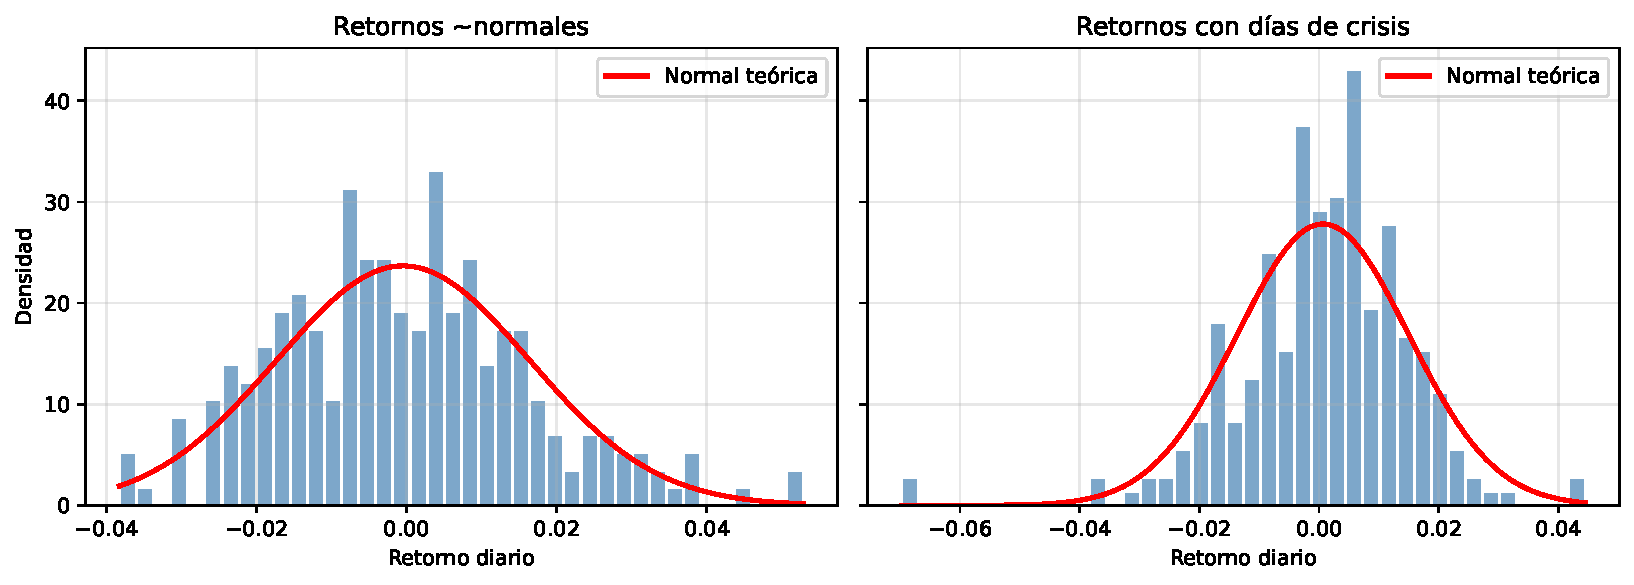
\includegraphics[keepaspectratio]{unidad2/cap07_estadistica_optimizacion_files/figure-pdf/histograma-output-1.pdf}}

En el panel derecho se ve la firma de los retornos financieros reales:
una \textbf{cola izquierda pesada} que la campana normal no alcanza a
cubrir. Los días de crisis existen, y la normal los declara casi
imposibles.

\section{Test de normalidad:
Jarque-Bera}\label{test-de-normalidad-jarque-bera}

El ojo engaña; mejor un test formal. El test de \textbf{Jarque-Bera}
pregunta exactamente lo que nos importa: \emph{¿la asimetría y la
curtosis de estos datos son compatibles con una distribución normal?} Su
hipótesis nula (\(H_0\)) es ``los datos son normales''.

La mecánica de decisión es la de cualquier test de hipótesis: si el
\textbf{p-value} es menor que el nivel de significancia (típicamente
\(\alpha = 0.05\)), rechazamos \(H_0\) --- los datos serían muy
improbables si la normal fuera cierta.

\phantomsection\label{jarque-bera}
\begin{Shaded}
\begin{Highlighting}[]
\ControlFlowTok{for}\NormalTok{ nombre, datos }\KeywordTok{in}\NormalTok{ [(}\StringTok{"Simulados normales"}\NormalTok{, retornos),}
\NormalTok{                      (}\StringTok{"Con días de crisis"}\NormalTok{, ret\_real)]:}
\NormalTok{    stat\_jb, p\_value }\OperatorTok{=}\NormalTok{ stats.jarque\_bera(datos)}
\NormalTok{    veredicto }\OperatorTok{=} \StringTok{"NO son normales"} \ControlFlowTok{if}\NormalTok{ p\_value }\OperatorTok{\textless{}} \FloatTok{0.05} \ControlFlowTok{else} \StringTok{"compatibles con normalidad"}
    \BuiltInTok{print}\NormalTok{(}\SpecialStringTok{f"}\SpecialCharTok{\{}\NormalTok{nombre}\SpecialCharTok{:\textless{}22\}}\SpecialStringTok{ JB=}\SpecialCharTok{\{}\NormalTok{stat\_jb}\SpecialCharTok{:8.2f\}}\SpecialStringTok{  p{-}value=}\SpecialCharTok{\{}\NormalTok{p\_value}\SpecialCharTok{:.4f\}}\SpecialStringTok{ → }\SpecialCharTok{\{}\NormalTok{veredicto}\SpecialCharTok{\}}\SpecialStringTok{"}\NormalTok{)}
\end{Highlighting}
\end{Shaded}

\begin{verbatim}
Simulados normales     JB=    6.47  p-value=0.0394 → NO son normales
Con días de crisis     JB=  185.49  p-value=0.0000 → NO son normales
\end{verbatim}

\begin{tcolorbox}[enhanced jigsaw, bottomrule=.15mm, colback=white, opacitybacktitle=0.6, arc=.35mm, toprule=.15mm, opacityback=0, breakable, titlerule=0mm, left=2mm, coltitle=black, colbacktitle=quarto-callout-warning-color!10!white, colframe=quarto-callout-warning-color-frame, leftrule=.75mm, toptitle=1mm, bottomtitle=1mm, title=\textcolor{quarto-callout-warning-color}{\faExclamationTriangle}\hspace{0.5em}{¿Y entonces por qué usamos la normal?}, rightrule=.15mm]

Si los retornos reales no son normales, ¿por qué media-varianza,
Black-Scholes y media industria asumen normalidad? Porque es
\textbf{tratable} y suele ser una aproximación razonable \emph{en el
centro} de la distribución. El problema aparece \textbf{en las colas}
--- justamente donde vive el riesgo extremo. Por eso el Módulo 3 dedica
capítulos enteros (VaR, Expected Shortfall, procesos con saltos) a medir
lo que la normal esconde. Usá la normal, pero sabiendo qué te está
simplificando.

\end{tcolorbox}

\begin{center}\rule{0.5\linewidth}{0.5pt}\end{center}

\chapter{Funciones lambda: el pegamento de la
optimización}\label{funciones-lambda-el-pegamento-de-la-optimizaciuxf3n}

Antes de optimizar, un mini-desvío de Python. Los optimizadores reciben
\emph{funciones} como argumentos, y muchas veces son funciones de una
sola línea que no ameritan un \texttt{def} con nombre. Para eso existen
las \textbf{lambdas}: funciones anónimas de una expresión.

\phantomsection\label{lambda}
\begin{Shaded}
\begin{Highlighting}[]
\CommentTok{\# Una función objetivo de juguete: una parábola con mínimo en x=3.5}
\NormalTok{funcion\_error }\OperatorTok{=} \KeywordTok{lambda}\NormalTok{ x: (x }\OperatorTok{{-}} \FloatTok{3.5}\NormalTok{) }\OperatorTok{**} \DecValTok{2} \OperatorTok{+} \DecValTok{2}

\ControlFlowTok{for}\NormalTok{ x }\KeywordTok{in}\NormalTok{ [}\DecValTok{0}\NormalTok{, }\DecValTok{2}\NormalTok{, }\FloatTok{3.5}\NormalTok{, }\DecValTok{5}\NormalTok{]:}
    \BuiltInTok{print}\NormalTok{(}\SpecialStringTok{f"f(}\SpecialCharTok{\{}\NormalTok{x}\SpecialCharTok{\}}\SpecialStringTok{) = }\SpecialCharTok{\{}\NormalTok{funcion\_error(x)}\SpecialCharTok{:.2f\}}\SpecialStringTok{"}\NormalTok{)}
\end{Highlighting}
\end{Shaded}

\begin{verbatim}
f(0) = 14.25
f(2) = 4.25
f(3.5) = 2.00
f(5) = 4.25
\end{verbatim}

Las vas a ver constantemente en las \textbf{restricciones} de los
optimizadores:
\texttt{\{"type":\ "eq",\ "fun":\ lambda\ w:\ w.sum()\ -\ 1\}} se lee
como ``la función \texttt{w.sum()\ -\ 1} debe valer cero'', es decir,
los pesos deben sumar 1.

\begin{center}\rule{0.5\linewidth}{0.5pt}\end{center}

\chapter{\texorpdfstring{Optimización con
\texttt{scipy.optimize}}{Optimización con scipy.optimize}}\label{optimizaciuxf3n-con-scipy.optimize}

\section{La idea: descenso guiado}\label{la-idea-descenso-guiado}

\texttt{minimize} recibe una función objetivo y un punto de partida, y
se mueve iterativamente ``cuesta abajo'' hasta encontrar un mínimo. No
necesitás decirle cómo: los algoritmos (usaremos \textbf{SLSQP}, que
soporta restricciones) estiman la pendiente y deciden el próximo paso.

\phantomsection\label{minimize-basico}
\begin{Shaded}
\begin{Highlighting}[]
\ImportTok{from}\NormalTok{ scipy.optimize }\ImportTok{import}\NormalTok{ minimize}

\CommentTok{\# Función de dos variables con mínimo en (3, 5)}
\KeywordTok{def}\NormalTok{ funcion\_objetivo(x):}
    \ControlFlowTok{return}\NormalTok{ (x[}\DecValTok{0}\NormalTok{] }\OperatorTok{{-}} \DecValTok{3}\NormalTok{) }\OperatorTok{**} \DecValTok{2} \OperatorTok{+}\NormalTok{ (x[}\DecValTok{1}\NormalTok{] }\OperatorTok{{-}} \DecValTok{5}\NormalTok{) }\OperatorTok{**} \DecValTok{2}

\NormalTok{resultado }\OperatorTok{=}\NormalTok{ minimize(funcion\_objetivo, x0}\OperatorTok{=}\NormalTok{[}\DecValTok{0}\NormalTok{, }\DecValTok{0}\NormalTok{], method}\OperatorTok{=}\StringTok{"SLSQP"}\NormalTok{)}

\BuiltInTok{print}\NormalTok{(}\SpecialStringTok{f"Mínimo encontrado en: x=}\SpecialCharTok{\{}\NormalTok{resultado}\SpecialCharTok{.}\NormalTok{x[}\DecValTok{0}\NormalTok{]}\SpecialCharTok{:.4f\}}\SpecialStringTok{, y=}\SpecialCharTok{\{}\NormalTok{resultado}\SpecialCharTok{.}\NormalTok{x[}\DecValTok{1}\NormalTok{]}\SpecialCharTok{:.4f\}}\SpecialStringTok{"}\NormalTok{)}
\BuiltInTok{print}\NormalTok{(}\SpecialStringTok{f"Valor mínimo: }\SpecialCharTok{\{}\NormalTok{resultado}\SpecialCharTok{.}\NormalTok{fun}\SpecialCharTok{:.6f\}}\SpecialStringTok{"}\NormalTok{)}
\BuiltInTok{print}\NormalTok{(}\SpecialStringTok{f"Convergió: }\SpecialCharTok{\{}\NormalTok{resultado}\SpecialCharTok{.}\NormalTok{success}\SpecialCharTok{\}}\SpecialStringTok{"}\NormalTok{)}
\end{Highlighting}
\end{Shaded}

\begin{verbatim}
Mínimo encontrado en: x=3.0000, y=5.0000
Valor mínimo: 0.000000
Convergió: True
\end{verbatim}

Tres cosas para mirar siempre en el resultado: \texttt{x} (dónde está el
óptimo), \texttt{fun} (cuánto vale la función ahí) y \texttt{success}
(si el algoritmo convergió --- \textbf{nunca uses un resultado sin
chequearlo}).

\begin{tcolorbox}[enhanced jigsaw, bottomrule=.15mm, colback=white, opacitybacktitle=0.6, arc=.35mm, toprule=.15mm, opacityback=0, breakable, titlerule=0mm, left=2mm, coltitle=black, colbacktitle=quarto-callout-tip-color!10!white, colframe=quarto-callout-tip-color-frame, leftrule=.75mm, toptitle=1mm, bottomtitle=1mm, title=\textcolor{quarto-callout-tip-color}{\faLightbulb}\hspace{0.5em}{Maximizar = minimizar el negativo}, rightrule=.15mm]

\texttt{scipy} solo minimiza. Cuando quieras \textbf{maximizar} algo
(utilidad, Sharpe), minimizá su negativo: max \(f(x)\) ⟺ min \(-f(x)\).
Por eso vas a ver funciones llamadas \texttt{utilidad\_negativa} o
\texttt{neg\_sharpe} en todo el libro.

\end{tcolorbox}

\section{Optimización con restricciones: primer portafolio
óptimo}\label{optimizaciuxf3n-con-restricciones-primer-portafolio-uxf3ptimo}

Ahora un problema financiero de verdad. Un inversor con \textbf{aversión
al riesgo} \(\lambda\) valora un portafolio según su utilidad
media-varianza:

\[U(\mathbf{w}) = \mathbf{w}^T\boldsymbol{\mu} - \frac{\lambda}{2}\, \mathbf{w}^T \Sigma \mathbf{w}\]

Es un balance explícito: el retorno suma, la varianza resta, y
\(\lambda\) regula cuánto pesa el miedo. Busquemos los pesos óptimos
para dos activos ---uno agresivo y uno defensivo--- con las
restricciones de siempre: pesos que suman 1, sin cortos.

\phantomsection\label{minimize-restricciones}
\begin{Shaded}
\begin{Highlighting}[]
\KeywordTok{def}\NormalTok{ utilidad\_negativa(w, mu, Sigma, aversion):}
    \CommentTok{"""Utilidad media{-}varianza, negada para minimizar."""}
\NormalTok{    ret\_port }\OperatorTok{=}\NormalTok{ w }\OperatorTok{@}\NormalTok{ mu}
\NormalTok{    var\_port }\OperatorTok{=}\NormalTok{ w }\OperatorTok{@}\NormalTok{ Sigma }\OperatorTok{@}\NormalTok{ w}
    \ControlFlowTok{return} \OperatorTok{{-}}\NormalTok{(ret\_port }\OperatorTok{{-}} \FloatTok{0.5} \OperatorTok{*}\NormalTok{ aversion }\OperatorTok{*}\NormalTok{ var\_port)}

\CommentTok{\# Dos activos: uno agresivo (10\%, vol 20\%) y uno defensivo (6\%, vol 10\%)}
\NormalTok{mu }\OperatorTok{=}\NormalTok{ np.array([}\FloatTok{0.10}\NormalTok{, }\FloatTok{0.06}\NormalTok{])}
\NormalTok{Sigma }\OperatorTok{=}\NormalTok{ np.array([[}\FloatTok{0.04}\NormalTok{, }\FloatTok{0.005}\NormalTok{],}
\NormalTok{                  [}\FloatTok{0.005}\NormalTok{, }\FloatTok{0.01}\NormalTok{]])}

\NormalTok{restricciones }\OperatorTok{=}\NormalTok{ [\{}\StringTok{"type"}\NormalTok{: }\StringTok{"eq"}\NormalTok{, }\StringTok{"fun"}\NormalTok{: }\KeywordTok{lambda}\NormalTok{ w: w.}\BuiltInTok{sum}\NormalTok{() }\OperatorTok{{-}} \DecValTok{1}\NormalTok{\}]}
\NormalTok{bounds }\OperatorTok{=}\NormalTok{ [(}\DecValTok{0}\NormalTok{, }\DecValTok{1}\NormalTok{)] }\OperatorTok{*} \DecValTok{2}

\ControlFlowTok{for}\NormalTok{ aversion }\KeywordTok{in}\NormalTok{ [}\DecValTok{1}\NormalTok{, }\DecValTok{3}\NormalTok{, }\DecValTok{10}\NormalTok{]:}
\NormalTok{    res }\OperatorTok{=}\NormalTok{ minimize(utilidad\_negativa, x0}\OperatorTok{=}\NormalTok{[}\FloatTok{0.5}\NormalTok{, }\FloatTok{0.5}\NormalTok{],}
\NormalTok{                   args}\OperatorTok{=}\NormalTok{(mu, Sigma, aversion),}
\NormalTok{                   method}\OperatorTok{=}\StringTok{"SLSQP"}\NormalTok{, bounds}\OperatorTok{=}\NormalTok{bounds, constraints}\OperatorTok{=}\NormalTok{restricciones)}
\NormalTok{    w }\OperatorTok{=}\NormalTok{ res.x}
    \BuiltInTok{print}\NormalTok{(}\SpecialStringTok{f"λ=}\SpecialCharTok{\{}\NormalTok{aversion}\SpecialCharTok{:\textgreater{}2\}}\SpecialStringTok{: agresivo }\SpecialCharTok{\{}\NormalTok{w[}\DecValTok{0}\NormalTok{]}\SpecialCharTok{:6.1\%\}}\SpecialStringTok{ | defensivo }\SpecialCharTok{\{}\NormalTok{w[}\DecValTok{1}\NormalTok{]}\SpecialCharTok{:6.1\%\}}\SpecialStringTok{"}
          \SpecialStringTok{f" | E[r]=}\SpecialCharTok{\{}\NormalTok{w }\OperatorTok{@}\NormalTok{ mu}\SpecialCharTok{:.2\%\}}\SpecialStringTok{ | vol=}\SpecialCharTok{\{}\NormalTok{np}\SpecialCharTok{.}\NormalTok{sqrt(w }\OperatorTok{@}\NormalTok{ Sigma }\OperatorTok{@}\NormalTok{ w)}\SpecialCharTok{:.2\%\}}\SpecialStringTok{"}\NormalTok{)}
\end{Highlighting}
\end{Shaded}

\begin{verbatim}
λ= 1: agresivo 100.0% | defensivo   0.0% | E[r]=10.00% | vol=20.00%
λ= 3: agresivo  45.8% | defensivo  54.2% | E[r]=7.83% | vol=11.76%
λ=10: agresivo  22.5% | defensivo  77.5% | E[r]=6.90% | vol=9.89%
\end{verbatim}

El resultado cuenta una historia coherente: a medida que sube la
aversión al riesgo, el óptimo \textbf{migra del activo agresivo al
defensivo}, sacrificando retorno esperado a cambio de menos volatilidad.
Tres inversores con la misma información y distinta tolerancia obtienen
tres carteras distintas --- y las tres son ``óptimas'' para quien las
tiene.

Este mecanismo ---función objetivo + restricciones +
\texttt{minimize}--- es exactamente el que escala a la \textbf{frontera
eficiente completa} del próximo capítulo. Ya tenés todas las piezas.

\begin{center}\rule{0.5\linewidth}{0.5pt}\end{center}

\chapter{Errores comunes}\label{errores-comunes-5}

\begin{tcolorbox}[enhanced jigsaw, bottomrule=.15mm, colback=white, opacitybacktitle=0.6, arc=.35mm, toprule=.15mm, opacityback=0, breakable, titlerule=0mm, left=2mm, coltitle=black, colbacktitle=quarto-callout-warning-color!10!white, colframe=quarto-callout-warning-color-frame, leftrule=.75mm, toptitle=1mm, bottomtitle=1mm, title=\textcolor{quarto-callout-warning-color}{\faExclamationTriangle}\hspace{0.5em}{Trampas frecuentes}, rightrule=.15mm]

\begin{itemize}
\tightlist
\item
  \textbf{No chequear \texttt{resultado.success}}: si el optimizador no
  convergió, \texttt{resultado.x} puede ser basura con aspecto
  respetable.
\item
  \textbf{Anualizar la volatilidad con ×252} en lugar de ×√252.
\item
  \textbf{Confundir curtosis con ``exceso de curtosis''}:
  \texttt{scipy.stats.kurtosis} devuelve el \emph{exceso} (normal = 0).
  Otras librerías devuelven la curtosis cruda (normal = 3).
\item
  \textbf{Interpretar un p-value alto como prueba de normalidad}: ``no
  rechazar \(H_0\)'' no es ``aceptar \(H_0\)''; con pocas observaciones,
  el test simplemente no tiene potencia para detectar la anormalidad.
\item
  \textbf{Punto de partida absurdo}: \texttt{minimize} es un buscador
  local. Con restricciones complejas, un \texttt{x0} razonable (p.~ej.,
  pesos equiponderados) evita óptimos locales o fallas de convergencia.
\end{itemize}

\end{tcolorbox}

\begin{center}\rule{0.5\linewidth}{0.5pt}\end{center}

\chapter{Ejercicios Propuestos}\label{ejercicios-propuestos-6}

\begin{tcolorbox}[enhanced jigsaw, bottomrule=.15mm, colback=white, opacitybacktitle=0.6, arc=.35mm, toprule=.15mm, opacityback=0, breakable, titlerule=0mm, left=2mm, coltitle=black, colbacktitle=quarto-callout-important-color!10!white, colframe=quarto-callout-important-color-frame, leftrule=.75mm, toptitle=1mm, bottomtitle=1mm, title=\textcolor{quarto-callout-important-color}{\faExclamation}\hspace{0.5em}{Ejercicios}, rightrule=.15mm]

\begin{enumerate}
\def\labelenumi{\arabic{enumi}.}
\tightlist
\item
  \textbf{Análisis comparado}: simulá (o descargá) retornos de 3 activos
  y armá una tabla con los cuatro momentos de cada uno. ¿Cuál elegirías
  por Sharpe? ¿Cambia tu respuesta al mirar la asimetría?
\item
  \textbf{Q-Q plot}: graficá un Q-Q plot (\texttt{stats.probplot}) de
  los retornos ``con crisis'' del capítulo. ¿Dónde se despegan los
  puntos de la recta?
\item
  \textbf{Shapiro-Wilk}: aplicá \texttt{stats.shapiro} además de
  Jarque-Bera a las dos series. ¿Coinciden los veredictos?
\item
  \textbf{Utilidad con 3 activos}: extendé el ejemplo de maximización de
  utilidad a 3 activos con una matriz de covarianzas 3×3, y barré
  \(\lambda\) de 1 a 10 graficando cómo evolucionan los pesos.
\item
  \textbf{Restricción extra}: agregá al problema anterior la restricción
  de que ningún activo supere el 50\% de la cartera y compará las
  soluciones.
\end{enumerate}

\end{tcolorbox}

Podés resolver estos ejercicios acá mismo: la celda ejecuta Python
\textbf{en tu navegador}, sin instalar nada (la primera ejecución tarda
unos segundos mientras carga el entorno; los paquetes que importes se
instalan solos).

\begin{Shaded}
\begin{Highlighting}[]
\NormalTok{\#| label: practica{-}navegador}
\NormalTok{import numpy as np}
\NormalTok{from scipy.optimize import minimize}
\NormalTok{from scipy import stats}

\NormalTok{\# Tu solución acá...}
\end{Highlighting}
\end{Shaded}

\begin{center}\rule{0.5\linewidth}{0.5pt}\end{center}

\chapter{Referencias}\label{referencias-6}

\phantomsection\label{refs}

\chapter{Capítulo 8: Teoría Moderna de Portafolios
(Markowitz)}\label{capuxedtulo-8-teoruxeda-moderna-de-portafolios-markowitz}

Frontera eficiente, métricas de desempeño y decisiones de diseño

El modelo de Markowitz formaliza la pregunta más importante de la
inversión: ¿cómo repartir el capital entre activos riesgosos?
Construimos la frontera eficiente con álgebra matricial y optimización
numérica, encontramos el portafolio de mínima varianza y el tangente, y
discutimos las decisiones que el paper de 1952 no responde: qué métrica
optimizar (Sharpe, Sortino, varianza), cómo tratar los dividendos, qué
rol juega la renta fija, cuándo trabajar con retornos reales y cuándo
con excesos de retorno.

\hfill\break

\chapter{Introducción}\label{introducciuxf3n-7}

Hasta ahora analizamos activos de a uno: su retorno, su volatilidad, su
distribución. Pero ningún inversor serio tiene un solo activo. La
pregunta real es otra: \textbf{¿cómo combinar activos para obtener el
mejor balance entre retorno y riesgo?}

En 1952, Harry Markowitz ---con 25 años--- respondió esa pregunta con
una idea que le valdría el Nobel: el riesgo de una cartera \textbf{no es
el promedio de los riesgos individuales}, porque los activos no se
mueven en sincronía perfecta. Cuando uno cae, otro puede subir. Esa
compensación ---la \textbf{covarianza}--- es la materia prima de la
diversificación, y puede medirse y optimizarse.

En este capítulo implementamos el modelo completo con NumPy y SciPy, y
después nos metemos en las decisiones prácticas que todo gestor enfrenta
y que el modelo básico deja abiertas.

\begin{tcolorbox}[enhanced jigsaw, bottomrule=.15mm, colback=white, opacitybacktitle=0.6, arc=.35mm, toprule=.15mm, opacityback=0, breakable, titlerule=0mm, left=2mm, coltitle=black, colbacktitle=quarto-callout-note-color!10!white, colframe=quarto-callout-note-color-frame, leftrule=.75mm, toptitle=1mm, bottomtitle=1mm, title=\textcolor{quarto-callout-note-color}{\faInfo}\hspace{0.5em}{Lo que ya sabés}, rightrule=.15mm]

Todo el andamiaje matemático de este capítulo ---producto matricial
\texttt{@}, matriz de covarianzas, la forma cuadrática
\(\mathbf{w}^T\Sigma\mathbf{w}\)--- lo construimos en el Capítulo 5
(NumPy). Y la herramienta de optimización,
\texttt{scipy.optimize.minimize}, la vimos en el Capítulo 7. Acá las
juntamos.

\end{tcolorbox}

\phantomsection\label{setup}
\begin{Shaded}
\begin{Highlighting}[]
\ImportTok{import}\NormalTok{ numpy }\ImportTok{as}\NormalTok{ np}
\ImportTok{import}\NormalTok{ matplotlib.pyplot }\ImportTok{as}\NormalTok{ plt}
\ImportTok{from}\NormalTok{ scipy.optimize }\ImportTok{import}\NormalTok{ minimize}

\NormalTok{np.set\_printoptions(precision}\OperatorTok{=}\DecValTok{4}\NormalTok{, suppress}\OperatorTok{=}\VariableTok{True}\NormalTok{)}
\NormalTok{rng }\OperatorTok{=}\NormalTok{ np.random.default\_rng(}\DecValTok{42}\NormalTok{)}
\end{Highlighting}
\end{Shaded}

\begin{center}\rule{0.5\linewidth}{0.5pt}\end{center}

\chapter{El problema en lenguaje
matricial}\label{el-problema-en-lenguaje-matricial}

Un portafolio de \(n\) activos queda definido por su vector de
\textbf{pesos} \(\mathbf{w} = (w_1, \dots, w_n)\), con \(\sum w_i = 1\).
Dadas las estimaciones de retornos esperados \(\boldsymbol{\mu}\) y la
matriz de covarianzas \(\Sigma\):

\begin{itemize}
\tightlist
\item
  \textbf{Retorno esperado del portafolio}:
  \(\ E[R_p] = \mathbf{w}^T \boldsymbol{\mu}\)
\item
  \textbf{Varianza del portafolio}:
  \(\ \sigma_p^2 = \mathbf{w}^T \Sigma \mathbf{w}\)
\end{itemize}

La segunda fórmula es la clave: incluye no solo las varianzas
individuales (la diagonal de \(\Sigma\)) sino \textbf{todas las
covarianzas cruzadas}. Ahí vive la diversificación.

\phantomsection\label{universo}
\begin{Shaded}
\begin{Highlighting}[]
\CommentTok{\# Universo de ejemplo: 4 activos con perfiles bien distintos}
\NormalTok{activos }\OperatorTok{=}\NormalTok{ [}\StringTok{"Acción Growth"}\NormalTok{, }\StringTok{"Acción Value"}\NormalTok{, }\StringTok{"Acción Defensiva"}\NormalTok{, }\StringTok{"Bono Corporativo"}\NormalTok{]}

\NormalTok{mu }\OperatorTok{=}\NormalTok{ np.array([}\FloatTok{0.14}\NormalTok{, }\FloatTok{0.10}\NormalTok{, }\FloatTok{0.07}\NormalTok{, }\FloatTok{0.05}\NormalTok{])      }\CommentTok{\# retornos esperados anuales}

\NormalTok{vols }\OperatorTok{=}\NormalTok{ np.array([}\FloatTok{0.28}\NormalTok{, }\FloatTok{0.20}\NormalTok{, }\FloatTok{0.14}\NormalTok{, }\FloatTok{0.06}\NormalTok{])    }\CommentTok{\# volatilidades anuales}
\NormalTok{corr }\OperatorTok{=}\NormalTok{ np.array([}
\NormalTok{    [}\FloatTok{1.00}\NormalTok{, }\FloatTok{0.65}\NormalTok{, }\FloatTok{0.45}\NormalTok{, }\FloatTok{0.10}\NormalTok{],}
\NormalTok{    [}\FloatTok{0.65}\NormalTok{, }\FloatTok{1.00}\NormalTok{, }\FloatTok{0.50}\NormalTok{, }\FloatTok{0.15}\NormalTok{],}
\NormalTok{    [}\FloatTok{0.45}\NormalTok{, }\FloatTok{0.50}\NormalTok{, }\FloatTok{1.00}\NormalTok{, }\FloatTok{0.20}\NormalTok{],}
\NormalTok{    [}\FloatTok{0.10}\NormalTok{, }\FloatTok{0.15}\NormalTok{, }\FloatTok{0.20}\NormalTok{, }\FloatTok{1.00}\NormalTok{],}
\NormalTok{])}
\NormalTok{Sigma }\OperatorTok{=}\NormalTok{ np.outer(vols, vols) }\OperatorTok{*}\NormalTok{ corr           }\CommentTok{\# Σ = D ρ D}

\CommentTok{\# Un portafolio cualquiera para arrancar}
\NormalTok{w }\OperatorTok{=}\NormalTok{ np.array([}\FloatTok{0.25}\NormalTok{, }\FloatTok{0.25}\NormalTok{, }\FloatTok{0.25}\NormalTok{, }\FloatTok{0.25}\NormalTok{])}

\NormalTok{ret\_p }\OperatorTok{=}\NormalTok{ w }\OperatorTok{@}\NormalTok{ mu}
\NormalTok{vol\_p }\OperatorTok{=}\NormalTok{ np.sqrt(w }\OperatorTok{@}\NormalTok{ Sigma }\OperatorTok{@}\NormalTok{ w)}

\BuiltInTok{print}\NormalTok{(}\SpecialStringTok{f"Portafolio equiponderado:"}\NormalTok{)}
\BuiltInTok{print}\NormalTok{(}\SpecialStringTok{f"  Retorno esperado: }\SpecialCharTok{\{}\NormalTok{ret\_p}\SpecialCharTok{:.2\%\}}\SpecialStringTok{"}\NormalTok{)}
\BuiltInTok{print}\NormalTok{(}\SpecialStringTok{f"  Volatilidad:      }\SpecialCharTok{\{}\NormalTok{vol\_p}\SpecialCharTok{:.2\%\}}\SpecialStringTok{"}\NormalTok{)}
\BuiltInTok{print}\NormalTok{(}\SpecialStringTok{f"  Promedio simple de vols individuales: }\SpecialCharTok{\{}\NormalTok{vols}\SpecialCharTok{.}\NormalTok{mean()}\SpecialCharTok{:.2\%\}}\SpecialStringTok{"}\NormalTok{)}
\end{Highlighting}
\end{Shaded}

\begin{verbatim}
Portafolio equiponderado:
  Retorno esperado: 9.00%
  Volatilidad:      13.42%
  Promedio simple de vols individuales: 17.00%
\end{verbatim}

Fijate el resultado: la volatilidad del portafolio es \textbf{menor que
el promedio de las volatilidades individuales}. No elegimos nada
inteligente todavía ---son pesos iguales--- y la diversificación ya nos
regaló varios puntos de riesgo. Eso es lo que Markowitz llamó \emph{the
only free lunch in finance}.

\begin{center}\rule{0.5\linewidth}{0.5pt}\end{center}

\chapter{La frontera eficiente}\label{la-frontera-eficiente}

De todos los portafolios posibles, ¿cuáles valen la pena? Markowitz lo
formuló como un problema de optimización: para cada nivel de retorno
objetivo \(\mu^*\), buscar los pesos que \textbf{minimizan la varianza}:

\[\min_{\mathbf{w}} \ \mathbf{w}^T \Sigma \mathbf{w} \quad \text{sujeto a} \quad \mathbf{w}^T \boldsymbol{\mu} = \mu^*, \quad \mathbf{w}^T \mathbf{1} = 1\]

El conjunto de soluciones dibuja una curva en el plano riesgo-retorno:
la \textbf{frontera eficiente}. Todo portafolio por debajo de ella es
mejorable (misma volatilidad, más retorno); por encima no hay nada
alcanzable.

\phantomsection\label{frontera}
\begin{Shaded}
\begin{Highlighting}[]
\KeywordTok{def}\NormalTok{ vol\_portafolio(w, Sigma):}
    \ControlFlowTok{return}\NormalTok{ np.sqrt(w }\OperatorTok{@}\NormalTok{ Sigma }\OperatorTok{@}\NormalTok{ w)}

\NormalTok{n }\OperatorTok{=} \BuiltInTok{len}\NormalTok{(mu)}
\NormalTok{w0 }\OperatorTok{=}\NormalTok{ np.ones(n) }\OperatorTok{/}\NormalTok{ n                      }\CommentTok{\# punto de partida: equiponderado}
\NormalTok{bounds }\OperatorTok{=}\NormalTok{ [(}\DecValTok{0}\NormalTok{, }\DecValTok{1}\NormalTok{)] }\OperatorTok{*}\NormalTok{ n                    }\CommentTok{\# sin ventas en corto}

\NormalTok{retornos\_objetivo }\OperatorTok{=}\NormalTok{ np.linspace(mu.}\BuiltInTok{min}\NormalTok{(), mu.}\BuiltInTok{max}\NormalTok{(), }\DecValTok{60}\NormalTok{)}
\NormalTok{frontera\_vol }\OperatorTok{=}\NormalTok{ []}
\NormalTok{frontera\_pesos }\OperatorTok{=}\NormalTok{ []}

\ControlFlowTok{for}\NormalTok{ r\_obj }\KeywordTok{in}\NormalTok{ retornos\_objetivo:}
\NormalTok{    restricciones }\OperatorTok{=}\NormalTok{ [}
\NormalTok{        \{}\StringTok{"type"}\NormalTok{: }\StringTok{"eq"}\NormalTok{, }\StringTok{"fun"}\NormalTok{: }\KeywordTok{lambda}\NormalTok{ w: w.}\BuiltInTok{sum}\NormalTok{() }\OperatorTok{{-}} \DecValTok{1}\NormalTok{\},}
\NormalTok{        \{}\StringTok{"type"}\NormalTok{: }\StringTok{"eq"}\NormalTok{, }\StringTok{"fun"}\NormalTok{: }\KeywordTok{lambda}\NormalTok{ w, r}\OperatorTok{=}\NormalTok{r\_obj: w }\OperatorTok{@}\NormalTok{ mu }\OperatorTok{{-}}\NormalTok{ r\},}
\NormalTok{    ]}
\NormalTok{    res }\OperatorTok{=}\NormalTok{ minimize(vol\_portafolio, w0, args}\OperatorTok{=}\NormalTok{(Sigma,),}
\NormalTok{                   method}\OperatorTok{=}\StringTok{"SLSQP"}\NormalTok{, bounds}\OperatorTok{=}\NormalTok{bounds, constraints}\OperatorTok{=}\NormalTok{restricciones)}
\NormalTok{    frontera\_vol.append(res.fun }\ControlFlowTok{if}\NormalTok{ res.success }\ControlFlowTok{else}\NormalTok{ np.nan)}
\NormalTok{    frontera\_pesos.append(res.x)}

\NormalTok{frontera\_vol }\OperatorTok{=}\NormalTok{ np.array(frontera\_vol)}
\end{Highlighting}
\end{Shaded}

\section{El portafolio de mínima varianza
global}\label{el-portafolio-de-muxednima-varianza-global}

Un punto especial de la frontera es su extremo izquierdo: el portafolio
de \textbf{mínima varianza global (GMV)}, el más conservador posible con
estos activos. No necesita estimar retornos esperados ---solo
\(\Sigma\)---, lo que lo hace más robusto que el resto de la frontera
(recordá: \(\boldsymbol{\mu}\) es lo más ruidoso).

\phantomsection\label{gmv}
\begin{Shaded}
\begin{Highlighting}[]
\NormalTok{res\_gmv }\OperatorTok{=}\NormalTok{ minimize(vol\_portafolio, w0, args}\OperatorTok{=}\NormalTok{(Sigma,),}
\NormalTok{                   method}\OperatorTok{=}\StringTok{"SLSQP"}\NormalTok{, bounds}\OperatorTok{=}\NormalTok{bounds,}
\NormalTok{                   constraints}\OperatorTok{=}\NormalTok{[\{}\StringTok{"type"}\NormalTok{: }\StringTok{"eq"}\NormalTok{, }\StringTok{"fun"}\NormalTok{: }\KeywordTok{lambda}\NormalTok{ w: w.}\BuiltInTok{sum}\NormalTok{() }\OperatorTok{{-}} \DecValTok{1}\NormalTok{\}])}
\NormalTok{w\_gmv }\OperatorTok{=}\NormalTok{ res\_gmv.x}

\BuiltInTok{print}\NormalTok{(}\StringTok{"Portafolio de Mínima Varianza Global:"}\NormalTok{)}
\ControlFlowTok{for}\NormalTok{ a, wi }\KeywordTok{in} \BuiltInTok{zip}\NormalTok{(activos, w\_gmv):}
    \BuiltInTok{print}\NormalTok{(}\SpecialStringTok{f"  }\SpecialCharTok{\{}\NormalTok{a}\SpecialCharTok{:\textless{}18\}}\SpecialStringTok{ }\SpecialCharTok{\{}\NormalTok{wi}\SpecialCharTok{:6.1\%\}}\SpecialStringTok{"}\NormalTok{)}
\BuiltInTok{print}\NormalTok{(}\SpecialStringTok{f"  Retorno: }\SpecialCharTok{\{}\NormalTok{w\_gmv }\OperatorTok{@}\NormalTok{ mu}\SpecialCharTok{:.2\%\}}\SpecialStringTok{ | Volatilidad: }\SpecialCharTok{\{}\NormalTok{res\_gmv}\SpecialCharTok{.}\NormalTok{fun}\SpecialCharTok{:.2\%\}}\SpecialStringTok{"}\NormalTok{)}
\end{Highlighting}
\end{Shaded}

\begin{verbatim}
Portafolio de Mínima Varianza Global:
  Acción Growth        0.0%
  Acción Value         1.3%
  Acción Defensiva     8.8%
  Bono Corporativo    89.9%
  Retorno: 5.24% | Volatilidad: 5.84%
\end{verbatim}

Como era de esperar, el GMV se carga hacia el bono (el activo menos
volátil) pero \textbf{no pone todo ahí}: mantiene algo de acciones
porque su baja correlación con el bono sigue restando riesgo total. La
diversificación manda incluso cuando solo minimizás varianza.

\section{El portafolio tangente y la Capital Market
Line}\label{el-portafolio-tangente-y-la-capital-market-line}

Ahora agreguemos un ingrediente: un \textbf{activo libre de riesgo} con
tasa \(r_f\) (un plazo fijo, una letra del tesoro). Poder combinar la
frontera con ese activo cambia la geometría del problema: las
combinaciones entre \(r_f\) y cualquier portafolio riesgoso son
\textbf{rectas} en el plano riesgo-retorno.

¿Cuál es la mejor recta? La que sale de \(r_f\) y \textbf{apenas toca}
la frontera: la \textbf{Capital Market Line (CML)}. El punto de
tangencia es el \textbf{portafolio tangente}, que maximiza el
\textbf{ratio de Sharpe}:

\[\text{Sharpe} = \frac{E[R_p] - r_f}{\sigma_p}\]

\phantomsection\label{tangente}
\begin{Shaded}
\begin{Highlighting}[]
\NormalTok{rf }\OperatorTok{=} \FloatTok{0.03}

\KeywordTok{def}\NormalTok{ neg\_sharpe(w, mu, Sigma, rf):}
    \ControlFlowTok{return} \OperatorTok{{-}}\NormalTok{(w }\OperatorTok{@}\NormalTok{ mu }\OperatorTok{{-}}\NormalTok{ rf) }\OperatorTok{/}\NormalTok{ np.sqrt(w }\OperatorTok{@}\NormalTok{ Sigma }\OperatorTok{@}\NormalTok{ w)}

\NormalTok{res\_tan }\OperatorTok{=}\NormalTok{ minimize(neg\_sharpe, w0, args}\OperatorTok{=}\NormalTok{(mu, Sigma, rf),}
\NormalTok{                   method}\OperatorTok{=}\StringTok{"SLSQP"}\NormalTok{, bounds}\OperatorTok{=}\NormalTok{bounds,}
\NormalTok{                   constraints}\OperatorTok{=}\NormalTok{[\{}\StringTok{"type"}\NormalTok{: }\StringTok{"eq"}\NormalTok{, }\StringTok{"fun"}\NormalTok{: }\KeywordTok{lambda}\NormalTok{ w: w.}\BuiltInTok{sum}\NormalTok{() }\OperatorTok{{-}} \DecValTok{1}\NormalTok{\}])}
\NormalTok{w\_tan }\OperatorTok{=}\NormalTok{ res\_tan.x}
\NormalTok{ret\_tan, vol\_tan }\OperatorTok{=}\NormalTok{ w\_tan }\OperatorTok{@}\NormalTok{ mu, np.sqrt(w\_tan }\OperatorTok{@}\NormalTok{ Sigma }\OperatorTok{@}\NormalTok{ w\_tan)}
\NormalTok{sharpe\_tan }\OperatorTok{=}\NormalTok{ (ret\_tan }\OperatorTok{{-}}\NormalTok{ rf) }\OperatorTok{/}\NormalTok{ vol\_tan}

\BuiltInTok{print}\NormalTok{(}\StringTok{"Portafolio Tangente (máximo Sharpe):"}\NormalTok{)}
\ControlFlowTok{for}\NormalTok{ a, wi }\KeywordTok{in} \BuiltInTok{zip}\NormalTok{(activos, w\_tan):}
    \BuiltInTok{print}\NormalTok{(}\SpecialStringTok{f"  }\SpecialCharTok{\{}\NormalTok{a}\SpecialCharTok{:\textless{}18\}}\SpecialStringTok{ }\SpecialCharTok{\{}\NormalTok{wi}\SpecialCharTok{:6.1\%\}}\SpecialStringTok{"}\NormalTok{)}
\BuiltInTok{print}\NormalTok{(}\SpecialStringTok{f"  Retorno: }\SpecialCharTok{\{}\NormalTok{ret\_tan}\SpecialCharTok{:.2\%\}}\SpecialStringTok{ | Vol: }\SpecialCharTok{\{}\NormalTok{vol\_tan}\SpecialCharTok{:.2\%\}}\SpecialStringTok{ | Sharpe: }\SpecialCharTok{\{}\NormalTok{sharpe\_tan}\SpecialCharTok{:.3f\}}\SpecialStringTok{"}\NormalTok{)}
\end{Highlighting}
\end{Shaded}

\begin{verbatim}
Portafolio Tangente (máximo Sharpe):
  Acción Growth       14.9%
  Acción Value         7.9%
  Acción Defensiva     6.1%
  Bono Corporativo    71.1%
  Retorno: 6.85% | Vol: 7.67% | Sharpe: 0.502
\end{verbatim}

\begin{Shaded}
\begin{Highlighting}[]
\NormalTok{fig, ax }\OperatorTok{=}\NormalTok{ plt.subplots(figsize}\OperatorTok{=}\NormalTok{(}\DecValTok{10}\NormalTok{, }\DecValTok{6}\NormalTok{))}

\CommentTok{\# Frontera eficiente}
\NormalTok{ax.plot(frontera\_vol }\OperatorTok{*} \DecValTok{100}\NormalTok{, retornos\_objetivo }\OperatorTok{*} \DecValTok{100}\NormalTok{, }\StringTok{"b{-}"}\NormalTok{, linewidth}\OperatorTok{=}\DecValTok{2}\NormalTok{,}
\NormalTok{        label}\OperatorTok{=}\StringTok{"Frontera eficiente"}\NormalTok{)}

\CommentTok{\# Capital Market Line: recta desde (0, rf) que pasa por el tangente}
\NormalTok{x\_cml }\OperatorTok{=}\NormalTok{ np.linspace(}\DecValTok{0}\NormalTok{, vol\_tan }\OperatorTok{*} \FloatTok{1.4}\NormalTok{, }\DecValTok{50}\NormalTok{)}
\NormalTok{ax.plot(x\_cml }\OperatorTok{*} \DecValTok{100}\NormalTok{, (rf }\OperatorTok{+}\NormalTok{ sharpe\_tan }\OperatorTok{*}\NormalTok{ x\_cml) }\OperatorTok{*} \DecValTok{100}\NormalTok{, }\StringTok{"g{-}{-}"}\NormalTok{, linewidth}\OperatorTok{=}\DecValTok{2}\NormalTok{,}
\NormalTok{        label}\OperatorTok{=}\StringTok{"Capital Market Line"}\NormalTok{)}

\CommentTok{\# Puntos notables}
\NormalTok{ax.scatter(vols }\OperatorTok{*} \DecValTok{100}\NormalTok{, mu }\OperatorTok{*} \DecValTok{100}\NormalTok{, s}\OperatorTok{=}\DecValTok{90}\NormalTok{, c}\OperatorTok{=}\StringTok{"red"}\NormalTok{, zorder}\OperatorTok{=}\DecValTok{5}\NormalTok{, label}\OperatorTok{=}\StringTok{"Activos individuales"}\NormalTok{)}
\ControlFlowTok{for}\NormalTok{ a, v, m }\KeywordTok{in} \BuiltInTok{zip}\NormalTok{(activos, vols, mu):}
\NormalTok{    ax.annotate(a, (v }\OperatorTok{*} \DecValTok{100}\NormalTok{, m }\OperatorTok{*} \DecValTok{100}\NormalTok{), textcoords}\OperatorTok{=}\StringTok{"offset points"}\NormalTok{,}
\NormalTok{                xytext}\OperatorTok{=}\NormalTok{(}\DecValTok{8}\NormalTok{, }\OperatorTok{{-}}\DecValTok{4}\NormalTok{), fontsize}\OperatorTok{=}\DecValTok{8}\NormalTok{)}
\NormalTok{ax.scatter(res\_gmv.fun }\OperatorTok{*} \DecValTok{100}\NormalTok{, (w\_gmv }\OperatorTok{@}\NormalTok{ mu) }\OperatorTok{*} \DecValTok{100}\NormalTok{, s}\OperatorTok{=}\DecValTok{160}\NormalTok{, c}\OperatorTok{=}\StringTok{"orange"}\NormalTok{, marker}\OperatorTok{=}\StringTok{"D"}\NormalTok{,}
\NormalTok{           zorder}\OperatorTok{=}\DecValTok{6}\NormalTok{, label}\OperatorTok{=}\StringTok{"Mínima varianza (GMV)"}\NormalTok{)}
\NormalTok{ax.scatter(vol\_tan }\OperatorTok{*} \DecValTok{100}\NormalTok{, ret\_tan }\OperatorTok{*} \DecValTok{100}\NormalTok{, s}\OperatorTok{=}\DecValTok{180}\NormalTok{, c}\OperatorTok{=}\StringTok{"green"}\NormalTok{, marker}\OperatorTok{=}\StringTok{"*"}\NormalTok{,}
\NormalTok{           zorder}\OperatorTok{=}\DecValTok{6}\NormalTok{, label}\OperatorTok{=}\StringTok{"Portafolio tangente"}\NormalTok{)}
\NormalTok{ax.scatter(}\DecValTok{0}\NormalTok{, rf }\OperatorTok{*} \DecValTok{100}\NormalTok{, s}\OperatorTok{=}\DecValTok{90}\NormalTok{, c}\OperatorTok{=}\StringTok{"black"}\NormalTok{, marker}\OperatorTok{=}\StringTok{"s"}\NormalTok{, zorder}\OperatorTok{=}\DecValTok{6}\NormalTok{,}
\NormalTok{           label}\OperatorTok{=}\SpecialStringTok{f"Libre de riesgo (}\SpecialCharTok{\{}\NormalTok{rf}\SpecialCharTok{:.0\%\}}\SpecialStringTok{)"}\NormalTok{)}

\NormalTok{ax.set\_xlabel(}\StringTok{"Volatilidad anual (\%)"}\NormalTok{)}
\NormalTok{ax.set\_ylabel(}\StringTok{"Retorno esperado anual (\%)"}\NormalTok{)}
\NormalTok{ax.set\_title(}\StringTok{"Frontera Eficiente, GMV, Tangente y CML"}\NormalTok{)}
\NormalTok{ax.legend(loc}\OperatorTok{=}\StringTok{"lower right"}\NormalTok{)}
\NormalTok{ax.grid(}\VariableTok{True}\NormalTok{, alpha}\OperatorTok{=}\FloatTok{0.3}\NormalTok{)}
\NormalTok{plt.tight\_layout()}
\NormalTok{plt.show()}
\end{Highlighting}
\end{Shaded}

\pandocbounded{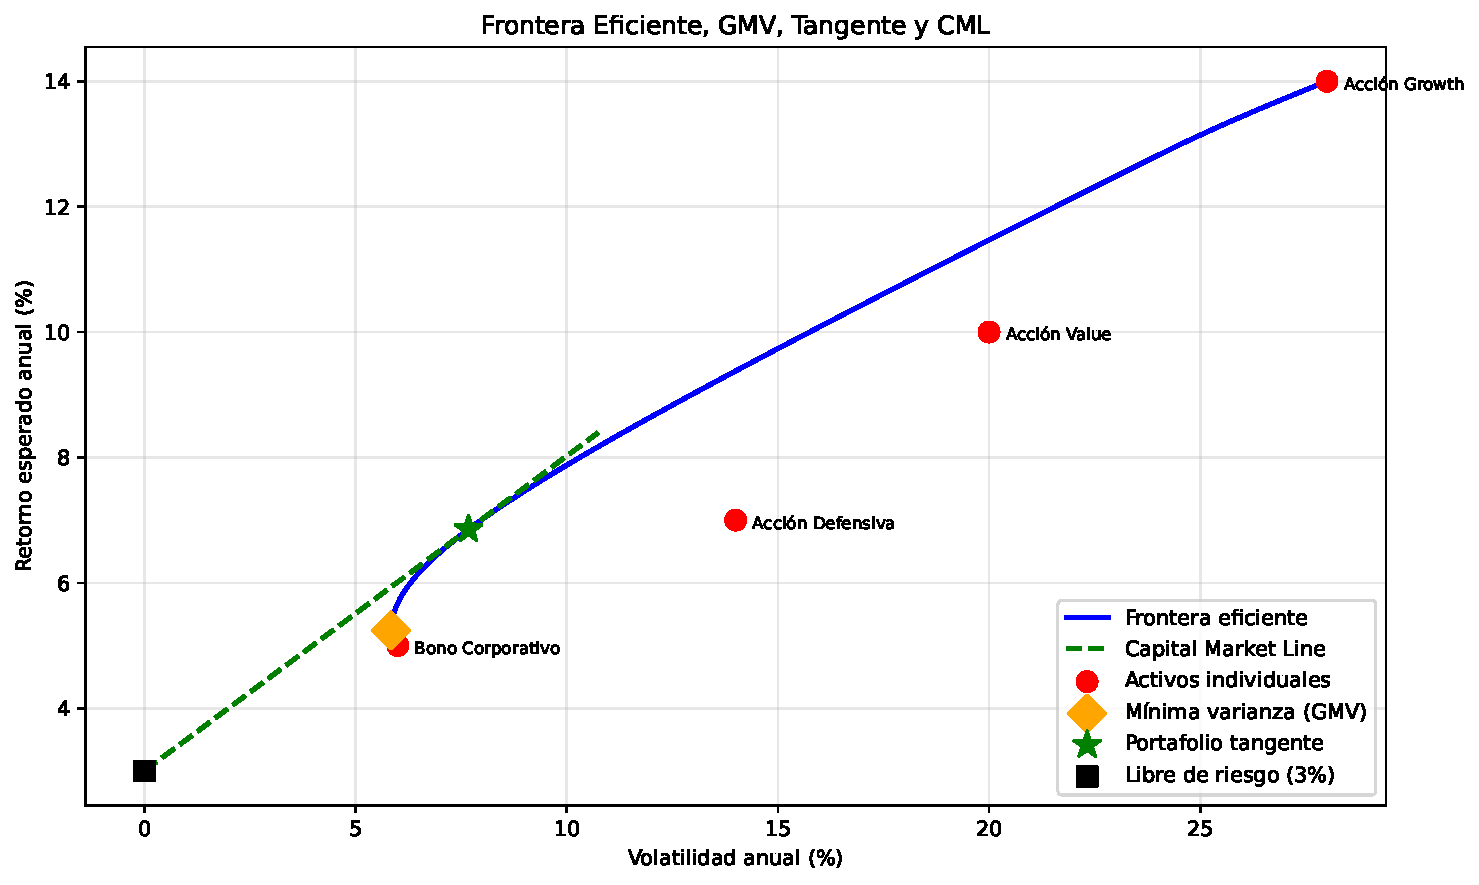
\includegraphics[keepaspectratio]{unidad2/cap08_markowitz_files/figure-pdf/grafico-frontera-output-1.pdf}}

La lectura del gráfico es una de las ideas más profundas de las
finanzas: \textbf{con un activo libre de riesgo disponible, la frontera
curva deja de ser el menú óptimo}. Todo inversor racional debería
pararse sobre la CML: elegir el portafolio tangente para su plata
riesgosa, y regular su nivel de riesgo total moviendo la proporción
entre el tangente y el activo libre de riesgo. El conservador pone 30\%
en el tangente y 70\% a tasa; el agresivo, todo en el tangente (o
incluso se apalanca). La \emph{composición} de la parte riesgosa es la
misma para ambos.

\begin{center}\rule{0.5\linewidth}{0.5pt}\end{center}

\chapter{¿Qué métrica optimizar? Sharpe, Sortino y
compañía}\label{quuxe9-muxe9trica-optimizar-sharpe-sortino-y-compauxf1uxeda}

Hasta acá maximizamos Sharpe como si fuera la única opción. No lo es, y
elegir la función objetivo es una \textbf{decisión de diseño} con
consecuencias. Repasemos el menú:

\begin{longtable}[]{@{}
  >{\raggedright\arraybackslash}p{(\linewidth - 4\tabcolsep) * \real{0.3333}}
  >{\raggedright\arraybackslash}p{(\linewidth - 4\tabcolsep) * \real{0.3333}}
  >{\raggedright\arraybackslash}p{(\linewidth - 4\tabcolsep) * \real{0.3333}}@{}}
\toprule\noalign{}
\begin{minipage}[b]{\linewidth}\raggedright
Objetivo
\end{minipage} & \begin{minipage}[b]{\linewidth}\raggedright
Qué premia / castiga
\end{minipage} & \begin{minipage}[b]{\linewidth}\raggedright
Cuándo tiene sentido
\end{minipage} \\
\midrule\noalign{}
\endhead
\bottomrule\noalign{}
\endlastfoot
\textbf{Mínima varianza} & Castiga toda dispersión, ignora el retorno &
Perfil ultraconservador; cuando desconfiás de tu estimación de
\(\mu\) \\
\textbf{Máximo retorno} & Ignora el riesgo por completo & Casi nunca
solo: lleva a concentrar todo en el activo más prometedor \\
\textbf{Máximo Sharpe} & Retorno en exceso por unidad de volatilidad
\emph{total} & El estándar de la industria para comparar estrategias \\
\textbf{Máximo Sortino} & Como Sharpe, pero solo castiga la volatilidad
\emph{a la baja} & Cuando la distribución es asimétrica y no querés
castigar las subas \\
\end{longtable}

El punto fino está entre Sharpe y Sortino. La volatilidad castiga
\textbf{ambas colas}: para el Sharpe, un activo que da sorpresas
positivas enormes es tan ``riesgoso'' como uno que se derrumba. El
\textbf{Sortino} corrige eso usando en el denominador solo la
\textbf{desviación a la baja} (\emph{downside deviation}), calculada con
los retornos por debajo de un umbral (típicamente \(r_f\) o cero):

\[\text{Sortino} = \frac{E[R_p] - r_f}{\sigma_{down}}, \qquad \sigma_{down} = \sqrt{\frac{1}{n}\sum_{r_i < \tau} (r_i - \tau)^2}\]

\phantomsection\label{sortino}
\begin{Shaded}
\begin{Highlighting}[]
\CommentTok{\# Simulamos la historia de dos estrategias con igual media y varianza...}
\NormalTok{n\_dias }\OperatorTok{=} \DecValTok{2500}
\NormalTok{r\_A }\OperatorTok{=}\NormalTok{ rng.normal(}\FloatTok{0.0005}\NormalTok{, }\FloatTok{0.012}\NormalTok{, n\_dias)                    }\CommentTok{\# simétrica}

\CommentTok{\# ...pero B tiene asimetría positiva: pierde poco seguido, gana mucho de a ratos}
\NormalTok{r\_B }\OperatorTok{=}\NormalTok{ rng.exponential(}\FloatTok{0.009}\NormalTok{, n\_dias) }\OperatorTok{{-}} \FloatTok{0.0085}
\NormalTok{r\_B }\OperatorTok{=}\NormalTok{ (r\_B }\OperatorTok{{-}}\NormalTok{ r\_B.mean()) }\OperatorTok{/}\NormalTok{ r\_B.std() }\OperatorTok{*} \FloatTok{0.012} \OperatorTok{+} \FloatTok{0.0005}      \CommentTok{\# igual media y desvío que A}

\NormalTok{rf\_diario }\OperatorTok{=} \FloatTok{0.03} \OperatorTok{/} \DecValTok{252}

\KeywordTok{def}\NormalTok{ sharpe\_anual(r):}
    \ControlFlowTok{return}\NormalTok{ (r.mean() }\OperatorTok{{-}}\NormalTok{ rf\_diario) }\OperatorTok{/}\NormalTok{ r.std() }\OperatorTok{*}\NormalTok{ np.sqrt(}\DecValTok{252}\NormalTok{)}

\KeywordTok{def}\NormalTok{ sortino\_anual(r, umbral}\OperatorTok{=}\NormalTok{rf\_diario):}
\NormalTok{    downside }\OperatorTok{=}\NormalTok{ np.sqrt(np.mean(np.minimum(r }\OperatorTok{{-}}\NormalTok{ umbral, }\DecValTok{0}\NormalTok{) }\OperatorTok{**} \DecValTok{2}\NormalTok{))}
    \ControlFlowTok{return}\NormalTok{ (r.mean() }\OperatorTok{{-}}\NormalTok{ umbral) }\OperatorTok{/}\NormalTok{ downside }\OperatorTok{*}\NormalTok{ np.sqrt(}\DecValTok{252}\NormalTok{)}

\BuiltInTok{print}\NormalTok{(}\SpecialStringTok{f"}\SpecialCharTok{\{}\StringTok{\textquotesingle{}\textquotesingle{}}\SpecialCharTok{:12\}\{}\StringTok{\textquotesingle{}Sharpe\textquotesingle{}}\SpecialCharTok{:\textgreater{}8\}\{}\StringTok{\textquotesingle{}Sortino\textquotesingle{}}\SpecialCharTok{:\textgreater{}9\}\{}\StringTok{\textquotesingle{}Asimetría\textquotesingle{}}\SpecialCharTok{:\textgreater{}11\}}\SpecialStringTok{"}\NormalTok{)}
\ControlFlowTok{for}\NormalTok{ nombre, r }\KeywordTok{in}\NormalTok{ [(}\StringTok{"Estrategia A"}\NormalTok{, r\_A), (}\StringTok{"Estrategia B"}\NormalTok{, r\_B)]:}
    \ImportTok{from}\NormalTok{ scipy }\ImportTok{import}\NormalTok{ stats}
    \BuiltInTok{print}\NormalTok{(}\SpecialStringTok{f"}\SpecialCharTok{\{}\NormalTok{nombre}\SpecialCharTok{:\textless{}12\}\{}\NormalTok{sharpe\_anual(r)}\SpecialCharTok{:\textgreater{}8.2f\}\{}\NormalTok{sortino\_anual(r)}\SpecialCharTok{:\textgreater{}9.2f\}}\SpecialStringTok{"}
          \SpecialStringTok{f"}\SpecialCharTok{\{}\NormalTok{stats}\SpecialCharTok{.}\NormalTok{skew(r)}\SpecialCharTok{:\textgreater{}11.2f\}}\SpecialStringTok{"}\NormalTok{)}
\end{Highlighting}
\end{Shaded}

\begin{verbatim}
              Sharpe  Sortino  Asimetría
Estrategia A   -0.20    -0.28      -0.04
Estrategia B    0.50     1.02       1.96
\end{verbatim}

Las dos estrategias tienen el mismo Sharpe (misma media, misma
varianza), pero el Sortino revela que \textbf{B pierde de manera más
contenida}: su riesgo ``malo'' es menor. Si tu inversor sufre las caídas
más de lo que disfruta las subas ---o sea, si es humano---, el Sortino
describe mejor su experiencia.

\begin{tcolorbox}[enhanced jigsaw, bottomrule=.15mm, colback=white, opacitybacktitle=0.6, arc=.35mm, toprule=.15mm, opacityback=0, breakable, titlerule=0mm, left=2mm, coltitle=black, colbacktitle=quarto-callout-tip-color!10!white, colframe=quarto-callout-tip-color-frame, leftrule=.75mm, toptitle=1mm, bottomtitle=1mm, title=\textcolor{quarto-callout-tip-color}{\faLightbulb}\hspace{0.5em}{¿Cuál usar?}, rightrule=.15mm]

No hay respuesta universal, pero sí una guía: \textbf{Sharpe para
comparar y comunicar} (todo el mundo lo entiende y lo calcula igual),
\textbf{Sortino cuando la asimetría importa} (estrategias con opciones,
crédito, o cualquier cosa con colas raras), \textbf{mínima varianza
cuando no confiás en tus retornos esperados}, y ``máximo retorno'' solo
como provocación intelectual. Y siempre mirá más de una métrica: cada
una ilumina un ángulo distinto.

\end{tcolorbox}

\begin{center}\rule{0.5\linewidth}{0.5pt}\end{center}

\chapter{Los inputs importan más que el
optimizador}\label{los-inputs-importan-muxe1s-que-el-optimizador}

El 90\% del esfuerzo práctico en Markowitz no está en la optimización
(eso lo hace \texttt{scipy} en milisegundos) sino en \textbf{estimar
bien \(\boldsymbol{\mu}\) y \(\Sigma\)}. Tres decisiones concretas que
cambian los resultados:

\section{Dividendos: usar retorno total, no solo
precio}\label{dividendos-usar-retorno-total-no-solo-precio}

El retorno de una acción tiene dos componentes: la variación del precio
\textbf{y los dividendos}. Ignorarlos ---un error común al bajar series
de precios sin ajustar--- subestima sistemáticamente \(\mu\):

\[R_{total} = \underbrace{\frac{P_t - P_{t-1}}{P_{t-1}}}_{\text{apreciación}} + \underbrace{\frac{D_t}{P_{t-1}}}_{\text{dividend yield}}\]

\phantomsection\label{dividendos}
\begin{Shaded}
\begin{Highlighting}[]
\CommentTok{\# Una acción "value" típica: sube poco de precio pero reparte 4\% anual}
\NormalTok{apreciacion }\OperatorTok{=} \FloatTok{0.05}
\NormalTok{dividend\_yield }\OperatorTok{=} \FloatTok{0.04}

\BuiltInTok{print}\NormalTok{(}\SpecialStringTok{f"Retorno solo{-}precio: }\SpecialCharTok{\{}\NormalTok{apreciacion}\SpecialCharTok{:.1\%\}}\SpecialStringTok{"}\NormalTok{)}
\BuiltInTok{print}\NormalTok{(}\SpecialStringTok{f"Retorno total:       }\SpecialCharTok{\{}\NormalTok{apreciacion }\OperatorTok{+}\NormalTok{ dividend\_yield}\SpecialCharTok{:.1\%\}}\SpecialStringTok{"}\NormalTok{)}

\CommentTok{\# En 20 años, la diferencia es enorme por capitalización:}
\BuiltInTok{print}\NormalTok{(}\SpecialStringTok{f"}\CharTok{\textbackslash{}n}\SpecialStringTok{$100 a 20 años, solo precio:   $}\SpecialCharTok{\{}\DecValTok{100} \OperatorTok{*}\NormalTok{ (}\DecValTok{1} \OperatorTok{+}\NormalTok{ apreciacion) }\OperatorTok{**} \DecValTok{20}\SpecialCharTok{:,.0f\}}\SpecialStringTok{"}\NormalTok{)}
\BuiltInTok{print}\NormalTok{(}\SpecialStringTok{f"$100 a 20 años, retorno total: $}\SpecialCharTok{\{}\DecValTok{100} \OperatorTok{*}\NormalTok{ (}\DecValTok{1} \OperatorTok{+}\NormalTok{ apreciacion }\OperatorTok{+}\NormalTok{ dividend\_yield) }\OperatorTok{**} \DecValTok{20}\SpecialCharTok{:,.0f\}}\SpecialStringTok{"}\NormalTok{)}
\end{Highlighting}
\end{Shaded}

\begin{verbatim}
Retorno solo-precio: 5.0%
Retorno total:       9.0%

$100 a 20 años, solo precio:   $265
$100 a 20 años, retorno total: $560
\end{verbatim}

Para un optimizador, esto no es un detalle: una acción de alto dividendo
puede parecer mediocre mirando solo el precio y ser excelente en retorno
total. \textbf{Usá siempre precios ajustados por dividendos}
(\emph{adjusted close}) o sumá el yield explícitamente.

\section{Renta fija en el universo: más que ``el activo sin
riesgo''}\label{renta-fija-en-el-universo-muxe1s-que-el-activo-sin-riesgo}

En el modelo de la CML, la renta fija aparece como el activo libre de
riesgo de volatilidad cero. Pero un \textbf{bono real} (como los que
valuamos en el Módulo 1) no es eso: tiene riesgo de tasa (duración),
riesgo de crédito y volatilidad de precio. La forma correcta de tratarlo
es \textbf{incluirlo como un activo riesgoso más} dentro del universo,
con su \(\mu\), su \(\sigma\) y ---lo más valioso--- su \textbf{baja
correlación} con las acciones.

Ya lo hicimos sin decirlo: nuestro cuarto activo es un bono corporativo.
Mirá cuánto aporta:

\begin{Shaded}
\begin{Highlighting}[]
\CommentTok{\# Frontera SIN el bono (solo los 3 primeros activos)}
\NormalTok{mu3, Sigma3 }\OperatorTok{=}\NormalTok{ mu[:}\DecValTok{3}\NormalTok{], Sigma[:}\DecValTok{3}\NormalTok{, :}\DecValTok{3}\NormalTok{]}
\NormalTok{w03 }\OperatorTok{=}\NormalTok{ np.ones(}\DecValTok{3}\NormalTok{) }\OperatorTok{/} \DecValTok{3}

\NormalTok{vols\_sin\_bono }\OperatorTok{=}\NormalTok{ []}
\NormalTok{rets\_grid }\OperatorTok{=}\NormalTok{ np.linspace(mu3.}\BuiltInTok{min}\NormalTok{(), mu3.}\BuiltInTok{max}\NormalTok{(), }\DecValTok{40}\NormalTok{)}
\ControlFlowTok{for}\NormalTok{ r\_obj }\KeywordTok{in}\NormalTok{ rets\_grid:}
\NormalTok{    res }\OperatorTok{=}\NormalTok{ minimize(vol\_portafolio, w03, args}\OperatorTok{=}\NormalTok{(Sigma3,), method}\OperatorTok{=}\StringTok{"SLSQP"}\NormalTok{,}
\NormalTok{                   bounds}\OperatorTok{=}\NormalTok{[(}\DecValTok{0}\NormalTok{, }\DecValTok{1}\NormalTok{)] }\OperatorTok{*} \DecValTok{3}\NormalTok{,}
\NormalTok{                   constraints}\OperatorTok{=}\NormalTok{[\{}\StringTok{"type"}\NormalTok{: }\StringTok{"eq"}\NormalTok{, }\StringTok{"fun"}\NormalTok{: }\KeywordTok{lambda}\NormalTok{ w: w.}\BuiltInTok{sum}\NormalTok{() }\OperatorTok{{-}} \DecValTok{1}\NormalTok{\},}
\NormalTok{                                \{}\StringTok{"type"}\NormalTok{: }\StringTok{"eq"}\NormalTok{, }\StringTok{"fun"}\NormalTok{: }\KeywordTok{lambda}\NormalTok{ w, r}\OperatorTok{=}\NormalTok{r\_obj: w }\OperatorTok{@}\NormalTok{ mu3 }\OperatorTok{{-}}\NormalTok{ r\}])}
\NormalTok{    vols\_sin\_bono.append(res.fun)}

\NormalTok{fig, ax }\OperatorTok{=}\NormalTok{ plt.subplots(figsize}\OperatorTok{=}\NormalTok{(}\DecValTok{9}\NormalTok{, }\DecValTok{5}\NormalTok{))}
\NormalTok{ax.plot(np.array(vols\_sin\_bono) }\OperatorTok{*} \DecValTok{100}\NormalTok{, rets\_grid }\OperatorTok{*} \DecValTok{100}\NormalTok{, }\StringTok{"r{-}{-}"}\NormalTok{, linewidth}\OperatorTok{=}\DecValTok{2}\NormalTok{,}
\NormalTok{        label}\OperatorTok{=}\StringTok{"Frontera sin bonos (solo acciones)"}\NormalTok{)}
\NormalTok{ax.plot(frontera\_vol }\OperatorTok{*} \DecValTok{100}\NormalTok{, retornos\_objetivo }\OperatorTok{*} \DecValTok{100}\NormalTok{, }\StringTok{"b{-}"}\NormalTok{, linewidth}\OperatorTok{=}\DecValTok{2}\NormalTok{,}
\NormalTok{        label}\OperatorTok{=}\StringTok{"Frontera con bonos"}\NormalTok{)}
\NormalTok{ax.set\_xlabel(}\StringTok{"Volatilidad anual (\%)"}\NormalTok{)}
\NormalTok{ax.set\_ylabel(}\StringTok{"Retorno esperado anual (\%)"}\NormalTok{)}
\NormalTok{ax.set\_title(}\StringTok{"El efecto de agregar renta fija al universo"}\NormalTok{)}
\NormalTok{ax.legend()}
\NormalTok{ax.grid(}\VariableTok{True}\NormalTok{, alpha}\OperatorTok{=}\FloatTok{0.3}\NormalTok{)}
\NormalTok{plt.tight\_layout()}
\NormalTok{plt.show()}
\end{Highlighting}
\end{Shaded}

\pandocbounded{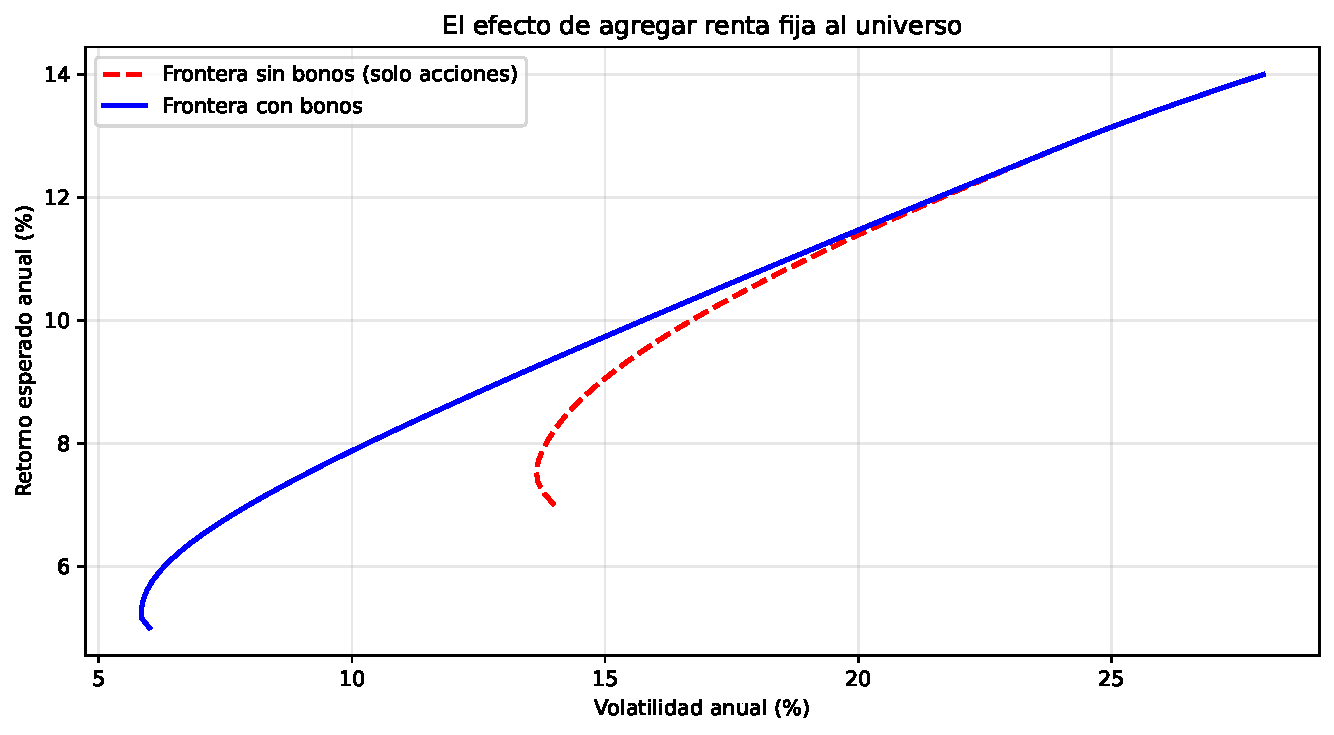
\includegraphics[keepaspectratio]{unidad2/cap08_markowitz_files/figure-pdf/bono-aporte-output-1.pdf}}

La frontera con bonos \textbf{domina} a la de solo-acciones en toda la
zona de riesgo bajo y medio: para los mismos retornos objetivo, menos
volatilidad. El bono no está ahí por su retorno (es el más bajo del
universo) sino por su \textbf{correlación baja}: es el mejor
diversificador de la mesa. Esta es la base cuantitativa del clásico
portafolio 60/40.

\section{Inflación y horizontes largos: deflactar o
engañarse}\label{inflaciuxf3n-y-horizontes-largos-deflactar-o-engauxf1arse}

Cuando el análisis abarca períodos largos ---décadas de historia, o
economías de alta inflación---, trabajar con retornos \textbf{nominales}
distorsiona todo. Un retorno nominal del 40\% anual con inflación del
45\% es una \textbf{pérdida} de poder adquisitivo, aunque el número se
vea espectacular. La conversión correcta es:

\[1 + r_{real} = \frac{1 + r_{nominal}}{1 + \pi} \quad\Rightarrow\quad r_{real} = \frac{r_{nominal} - \pi}{1 + \pi}\]

\phantomsection\label{deflactar}
\begin{Shaded}
\begin{Highlighting}[]
\NormalTok{casos }\OperatorTok{=}\NormalTok{ [}
\NormalTok{    (}\StringTok{"EEUU, año típico"}\NormalTok{, }\FloatTok{0.10}\NormalTok{, }\FloatTok{0.03}\NormalTok{),}
\NormalTok{    (}\StringTok{"Argentina, año de alta inflación"}\NormalTok{, }\FloatTok{0.40}\NormalTok{, }\FloatTok{0.45}\NormalTok{),}
\NormalTok{    (}\StringTok{"Argentina, buen año real"}\NormalTok{, }\FloatTok{0.80}\NormalTok{, }\FloatTok{0.50}\NormalTok{),}
\NormalTok{]}

\BuiltInTok{print}\NormalTok{(}\SpecialStringTok{f"}\SpecialCharTok{\{}\StringTok{\textquotesingle{}Caso\textquotesingle{}}\SpecialCharTok{:\textless{}34\}\{}\StringTok{\textquotesingle{}Nominal\textquotesingle{}}\SpecialCharTok{:\textgreater{}9\}\{}\StringTok{\textquotesingle{}Inflación\textquotesingle{}}\SpecialCharTok{:\textgreater{}11\}\{}\StringTok{\textquotesingle{}Real\textquotesingle{}}\SpecialCharTok{:\textgreater{}8\}}\SpecialStringTok{"}\NormalTok{)}
\ControlFlowTok{for}\NormalTok{ nombre, r\_nom, pi }\KeywordTok{in}\NormalTok{ casos:}
\NormalTok{    r\_real }\OperatorTok{=}\NormalTok{ (r\_nom }\OperatorTok{{-}}\NormalTok{ pi) }\OperatorTok{/}\NormalTok{ (}\DecValTok{1} \OperatorTok{+}\NormalTok{ pi)}
    \BuiltInTok{print}\NormalTok{(}\SpecialStringTok{f"}\SpecialCharTok{\{}\NormalTok{nombre}\SpecialCharTok{:\textless{}34\}\{}\NormalTok{r\_nom}\SpecialCharTok{:\textgreater{}8.0\%\}\{}\NormalTok{pi}\SpecialCharTok{:\textgreater{}10.0\%\}\{}\NormalTok{r\_real}\SpecialCharTok{:\textgreater{}8.1\%\}}\SpecialStringTok{"}\NormalTok{)}
\end{Highlighting}
\end{Shaded}

\begin{verbatim}
Caso                                Nominal  Inflación    Real
EEUU, año típico                       10%        3%    6.8%
Argentina, año de alta inflación       40%       45%   -3.4%
Argentina, buen año real               80%       50%   20.0%
\end{verbatim}

¿Por qué importa para Markowitz? Porque en series largas o
inflacionarias, la inflación \textbf{infla artificialmente las medias y
las correlaciones}: todos los activos ``suben'' juntos con el nivel de
precios, y el optimizador cree ver retornos altos y co-movimientos que
no existen en términos reales. La regla práctica:

\begin{itemize}
\tightlist
\item
  \textbf{Horizontes cortos y baja inflación} (retornos
  diarios/mensuales en economías estables): trabajar en nominal es
  aceptable; la inflación es un ruido de fondo casi constante.
\item
  \textbf{Horizontes largos o alta inflación}: deflactá las series (o
  trabajá en una moneda dura de referencia) \emph{antes} de estimar
  \(\mu\) y \(\Sigma\). Lo que le importa al inversor es el poder de
  compra, no los pesos nominales.
\end{itemize}

\section{¿Retornos directos o excesos de
retorno?}\label{retornos-directos-o-excesos-de-retorno}

Última decisión de diseño: ¿optimizamos sobre los retornos ``crudos'' de
cada activo, o sobre su \textbf{exceso} respecto de una referencia
(\(r_i - r_f\), o \(r_i - r_{mkt}\))? La respuesta depende de qué
pregunta estés haciendo:

\begin{itemize}
\tightlist
\item
  \textbf{Retornos directos (o reales)} --- cuando la pregunta es de
  \textbf{asignación de capital total}: ``tengo \(X\), ¿cómo lo
  reparto?''. El nivel absoluto de cada retorno importa, porque la
  alternativa de no invertir (o de quedarse en tasa) es parte del
  problema. La frontera y la CML de este capítulo trabajan así.
\item
  \textbf{Excesos sobre la tasa libre de riesgo} (\(r_i - r_f\)) ---
  cuando la tasa varía en el tiempo y querés que tu estimación de
  \(\mu\) no mezcle ``premio por riesgo'' con ``nivel de tasas''. El
  ratio de Sharpe ya está definido sobre excesos; estimar directamente
  en excesos hace todo más consistente, especialmente con datos que
  cruzan regímenes de tasas muy distintos.
\item
  \textbf{Excesos sobre el mercado} (\(r_i - r_{mkt}\)) --- cuando el
  problema no es asignar capital sino \textbf{construir una cartera
  activa} que le gane a un benchmark. Ahí lo que optimizás es el
  \emph{tracking error} y el exceso de retorno relativo; el riesgo ``de
  mercado'' es irrelevante porque el benchmark ya lo carga. Es el mundo
  de los fondos con mandato relativo.
\end{itemize}

\begin{tcolorbox}[enhanced jigsaw, bottomrule=.15mm, colback=white, opacitybacktitle=0.6, arc=.35mm, toprule=.15mm, opacityback=0, breakable, titlerule=0mm, left=2mm, coltitle=black, colbacktitle=quarto-callout-warning-color!10!white, colframe=quarto-callout-warning-color-frame, leftrule=.75mm, toptitle=1mm, bottomtitle=1mm, title=\textcolor{quarto-callout-warning-color}{\faExclamationTriangle}\hspace{0.5em}{El error clásico}, rightrule=.15mm]

Mezclar marcos: estimar \(\mu\) como promedio de retornos nominales de
una década de tasas altas, y usarlo para optimizar hoy con tasas bajas.
El ``premio'' que el optimizador ve es en gran parte nivel de tasas que
ya no existe. Trabajar en excesos sobre \(r_f\) inmuniza contra esto.

\end{tcolorbox}

\begin{center}\rule{0.5\linewidth}{0.5pt}\end{center}

\chapter{Las limitaciones del modelo (y adónde
vamos)}\label{las-limitaciones-del-modelo-y-aduxf3nde-vamos}

Markowitz es el punto de partida de toda la teoría de portafolios, pero
conviene salir del capítulo con sus límites claros:

\begin{enumerate}
\def\labelenumi{\arabic{enumi}.}
\tightlist
\item
  \textbf{Hipersensibilidad a los inputs}: cambios chicos en
  \(\boldsymbol{\mu}\) producen carteras completamente distintas, y
  \(\boldsymbol{\mu}\) es casi imposible de estimar bien. Es el problema
  que atacan \textbf{HRP} (capítulo siguiente, esquivando la inversión
  de \(\Sigma\)) y \textbf{Black-Litterman} (Capítulo 10, disciplinando
  la estimación de \(\mu\)).
\item
  \textbf{Supone que la varianza captura el riesgo}: ignora asimetrías y
  colas pesadas. Las métricas de cola (VaR, Expected Shortfall) llegan
  en el Módulo 3.
\item
  \textbf{Un solo período}: el modelo decide una vez y se queda quieto;
  no contempla rebalanceo, costos de transacción ni impuestos.
\item
  \textbf{Las correlaciones no son constantes}: en las crisis, justo
  cuando más importa, las correlaciones suben y la diversificación se
  evapora. Lo veremos con crudeza en el capítulo de riesgo y regulación.
\end{enumerate}

Nada de esto ``refuta'' a Markowitz: define la agenda de todo lo que
sigue en el libro.

\begin{center}\rule{0.5\linewidth}{0.5pt}\end{center}

\chapter{Con datos reales}\label{con-datos-reales}

Todo el capítulo trabajó con un universo inventado de 4 activos, donde
nosotros elegimos \(\boldsymbol{\mu}\) y \(\Sigma\). Cerremos con el
ejercicio completo sobre \textbf{datos de mercado}: el libro incluye en
\href{https://github.com/diegoonna/libro_finanzas_computacionales/blob/main/datos/precios.csv}{\texttt{datos/precios.csv}}
cinco años de precios diarios ajustados (jul-2021 a jun-2026) de 9
acciones de sectores distintos más el ETF SPY (ver el
Apéndice~\ref{sec-datos-financieros} para los detalles del dataset).

\phantomsection\label{datos-reales}
\begin{Shaded}
\begin{Highlighting}[]
\ImportTok{import}\NormalTok{ pandas }\ImportTok{as}\NormalTok{ pd}

\NormalTok{precios }\OperatorTok{=}\NormalTok{ pd.read\_csv(}\StringTok{"../datos/precios.csv"}\NormalTok{, index\_col}\OperatorTok{=}\StringTok{"Date"}\NormalTok{, parse\_dates}\OperatorTok{=}\VariableTok{True}\NormalTok{)}
\NormalTok{acciones }\OperatorTok{=}\NormalTok{ [c }\ControlFlowTok{for}\NormalTok{ c }\KeywordTok{in}\NormalTok{ precios.columns }\ControlFlowTok{if}\NormalTok{ c }\OperatorTok{!=} \StringTok{"SPY"}\NormalTok{]   }\CommentTok{\# SPY lo reservamos como "mercado"}

\CommentTok{\# Retornos mensuales (más estables que los diarios para estimar μ)}
\NormalTok{r\_mensual }\OperatorTok{=}\NormalTok{ precios[acciones].resample(}\StringTok{"ME"}\NormalTok{).last().pct\_change().dropna()}

\NormalTok{mu\_real }\OperatorTok{=}\NormalTok{ r\_mensual.mean().values }\OperatorTok{*} \DecValTok{12}                  \CommentTok{\# anualizado}
\NormalTok{Sigma\_real }\OperatorTok{=}\NormalTok{ r\_mensual.cov().values }\OperatorTok{*} \DecValTok{12}

\BuiltInTok{print}\NormalTok{(}\SpecialStringTok{f"Observaciones mensuales: }\SpecialCharTok{\{}\BuiltInTok{len}\NormalTok{(r\_mensual)}\SpecialCharTok{\}}\SpecialStringTok{"}\NormalTok{)}
\BuiltInTok{print}\NormalTok{(}\SpecialStringTok{f"}\SpecialCharTok{\{}\StringTok{\textquotesingle{}Ticker\textquotesingle{}}\SpecialCharTok{:\textless{}8\}\{}\StringTok{\textquotesingle{}μ anual\textquotesingle{}}\SpecialCharTok{:\textgreater{}9\}\{}\StringTok{\textquotesingle{}σ anual\textquotesingle{}}\SpecialCharTok{:\textgreater{}9\}}\SpecialStringTok{"}\NormalTok{)}
\ControlFlowTok{for}\NormalTok{ t, m, s }\KeywordTok{in} \BuiltInTok{zip}\NormalTok{(acciones, mu\_real, np.sqrt(np.diag(Sigma\_real))):}
    \BuiltInTok{print}\NormalTok{(}\SpecialStringTok{f"}\SpecialCharTok{\{}\NormalTok{t}\SpecialCharTok{:\textless{}8\}\{}\NormalTok{m}\SpecialCharTok{:\textgreater{}8.1\%\}\{}\NormalTok{s}\SpecialCharTok{:\textgreater{}9.1\%\}}\SpecialStringTok{"}\NormalTok{)}
\end{Highlighting}
\end{Shaded}

\begin{verbatim}
Observaciones mensuales: 59
Ticker    μ anual  σ anual
AAPL       17.1%    25.3%
MSFT        9.3%    25.6%
NVDA       60.3%    51.0%
JPM        21.1%    24.0%
XOM        24.8%    27.0%
KO         11.9%    16.5%
JNJ        12.8%    18.4%
WMT        21.5%    20.7%
DIS        -6.0%    33.2%
\end{verbatim}

Con \(\boldsymbol{\mu}\) y \(\Sigma\) estimados, el resto es exactamente
el código que ya escribimos:

\phantomsection\label{datos-reales-optimizacion}
\begin{Shaded}
\begin{Highlighting}[]
\NormalTok{n\_r }\OperatorTok{=} \BuiltInTok{len}\NormalTok{(acciones)}
\NormalTok{w0\_r }\OperatorTok{=}\NormalTok{ np.ones(n\_r) }\OperatorTok{/}\NormalTok{ n\_r}
\NormalTok{bounds\_r }\OperatorTok{=}\NormalTok{ [(}\DecValTok{0}\NormalTok{, }\DecValTok{1}\NormalTok{)] }\OperatorTok{*}\NormalTok{ n\_r}

\CommentTok{\# GMV}
\NormalTok{res\_gmv\_r }\OperatorTok{=}\NormalTok{ minimize(vol\_portafolio, w0\_r, args}\OperatorTok{=}\NormalTok{(Sigma\_real,),}
\NormalTok{                     method}\OperatorTok{=}\StringTok{"SLSQP"}\NormalTok{, bounds}\OperatorTok{=}\NormalTok{bounds\_r,}
\NormalTok{                     constraints}\OperatorTok{=}\NormalTok{[\{}\StringTok{"type"}\NormalTok{: }\StringTok{"eq"}\NormalTok{, }\StringTok{"fun"}\NormalTok{: }\KeywordTok{lambda}\NormalTok{ w: w.}\BuiltInTok{sum}\NormalTok{() }\OperatorTok{{-}} \DecValTok{1}\NormalTok{\}])}

\CommentTok{\# Tangente}
\NormalTok{res\_tan\_r }\OperatorTok{=}\NormalTok{ minimize(neg\_sharpe, w0\_r, args}\OperatorTok{=}\NormalTok{(mu\_real, Sigma\_real, rf),}
\NormalTok{                     method}\OperatorTok{=}\StringTok{"SLSQP"}\NormalTok{, bounds}\OperatorTok{=}\NormalTok{bounds\_r,}
\NormalTok{                     constraints}\OperatorTok{=}\NormalTok{[\{}\StringTok{"type"}\NormalTok{: }\StringTok{"eq"}\NormalTok{, }\StringTok{"fun"}\NormalTok{: }\KeywordTok{lambda}\NormalTok{ w: w.}\BuiltInTok{sum}\NormalTok{() }\OperatorTok{{-}} \DecValTok{1}\NormalTok{\}])}

\BuiltInTok{print}\NormalTok{(}\SpecialStringTok{f"}\SpecialCharTok{\{}\StringTok{\textquotesingle{}Ticker\textquotesingle{}}\SpecialCharTok{:\textless{}8\}\{}\StringTok{\textquotesingle{}GMV\textquotesingle{}}\SpecialCharTok{:\textgreater{}8\}\{}\StringTok{\textquotesingle{}Tangente\textquotesingle{}}\SpecialCharTok{:\textgreater{}10\}}\SpecialStringTok{"}\NormalTok{)}
\ControlFlowTok{for}\NormalTok{ t, wg, wt }\KeywordTok{in} \BuiltInTok{zip}\NormalTok{(acciones, res\_gmv\_r.x, res\_tan\_r.x):}
    \BuiltInTok{print}\NormalTok{(}\SpecialStringTok{f"}\SpecialCharTok{\{}\NormalTok{t}\SpecialCharTok{:\textless{}8\}\{}\NormalTok{wg}\SpecialCharTok{:\textgreater{}8.1\%\}\{}\NormalTok{wt}\SpecialCharTok{:\textgreater{}10.1\%\}}\SpecialStringTok{"}\NormalTok{)}

\NormalTok{ret\_tan\_r }\OperatorTok{=}\NormalTok{ res\_tan\_r.x }\OperatorTok{@}\NormalTok{ mu\_real}
\NormalTok{vol\_tan\_r }\OperatorTok{=}\NormalTok{ np.sqrt(res\_tan\_r.x }\OperatorTok{@}\NormalTok{ Sigma\_real }\OperatorTok{@}\NormalTok{ res\_tan\_r.x)}
\BuiltInTok{print}\NormalTok{(}\SpecialStringTok{f"}\CharTok{\textbackslash{}n}\SpecialStringTok{Tangente: retorno }\SpecialCharTok{\{}\NormalTok{ret\_tan\_r}\SpecialCharTok{:.1\%\}}\SpecialStringTok{, vol }\SpecialCharTok{\{}\NormalTok{vol\_tan\_r}\SpecialCharTok{:.1\%\}}\SpecialStringTok{, "}
      \SpecialStringTok{f"Sharpe }\SpecialCharTok{\{}\NormalTok{(ret\_tan\_r }\OperatorTok{{-}}\NormalTok{ rf) }\OperatorTok{/}\NormalTok{ vol\_tan\_r}\SpecialCharTok{:.2f\}}\SpecialStringTok{"}\NormalTok{)}
\end{Highlighting}
\end{Shaded}

\begin{verbatim}
Ticker       GMV  Tangente
AAPL        1.6%      0.0%
MSFT       23.1%      0.0%
NVDA        0.0%     23.3%
JPM         4.8%      0.0%
XOM        13.4%     29.2%
KO         19.3%      5.4%
JNJ        27.9%     17.9%
WMT         9.9%     24.2%
DIS         0.0%      0.0%

Tangente: retorno 29.4%, vol 16.9%, Sharpe 1.57
\end{verbatim}

El resultado ilustra en carne propia las advertencias del capítulo. Mirá
primero la tabla de \(\mu\) estimados: NVDA con un retorno anualizado
altísimo (la ola de la IA cayó entera dentro de la ventana), DIS en
terreno negativo. El portafolio tangente \textbf{se toma esos números al
pie de la letra}: asigna cero a más de la mitad del universo y concentra
el capital en los cuatro o cinco tickers que mejor combinaron retorno y
volatilidad \emph{en esa muestra}. ¿De verdad creés que NVDA va a
repetir ese μ los próximos cinco años? El optimizador sí. El GMV, que no
usa \(\boldsymbol{\mu}\), queda bastante más repartido y cargado en los
activos defensivos. Esa fragilidad frente al \(\mu\) estimado es
exactamente el problema que atacan HRP (capítulo siguiente) y
Black-Litterman (Capítulo 10) --- y ahora la viste con datos de verdad.

\begin{center}\rule{0.5\linewidth}{0.5pt}\end{center}

\chapter{Errores comunes}\label{errores-comunes-6}

\begin{tcolorbox}[enhanced jigsaw, bottomrule=.15mm, colback=white, opacitybacktitle=0.6, arc=.35mm, toprule=.15mm, opacityback=0, breakable, titlerule=0mm, left=2mm, coltitle=black, colbacktitle=quarto-callout-warning-color!10!white, colframe=quarto-callout-warning-color-frame, leftrule=.75mm, toptitle=1mm, bottomtitle=1mm, title=\textcolor{quarto-callout-warning-color}{\faExclamationTriangle}\hspace{0.5em}{Trampas frecuentes}, rightrule=.15mm]

\begin{itemize}
\tightlist
\item
  \textbf{Anualizar mal}: los retornos escalan por \(T\) (×252 de diario
  a anual) pero la volatilidad escala por \(\sqrt{T}\)
  (×\(\sqrt{252}\)). Mezclar las dos reglas rompe todos los ratios.
\item
  \textbf{Usar precios sin ajustar por dividendos}: subestima el retorno
  de los activos de alto yield y sesga la optimización hacia las
  acciones growth.
\item
  \textbf{Olvidar las restricciones}: sin \texttt{bounds={[}(0,1){]}},
  el optimizador puede sugerir ventas en corto del 300\%. Verificá
  siempre que la solución sea implementable.
\item
  \textbf{Confiar en un único punto de partida}: \texttt{minimize} puede
  quedar atrapado en óptimos locales con restricciones complejas. Ante
  dudas, probá varios \texttt{w0}.
\item
  \textbf{Interpretar la frontera como predicción}: la frontera es
  óptima \emph{para las estimaciones que le diste}. Si \(\mu\) y
  \(\Sigma\) están mal, la frontera es una ficción precisa.
\end{itemize}

\end{tcolorbox}

\begin{center}\rule{0.5\linewidth}{0.5pt}\end{center}

\chapter{Ejercicios Propuestos}\label{ejercicios-propuestos-7}

\begin{tcolorbox}[enhanced jigsaw, bottomrule=.15mm, colback=white, opacitybacktitle=0.6, arc=.35mm, toprule=.15mm, opacityback=0, breakable, titlerule=0mm, left=2mm, coltitle=black, colbacktitle=quarto-callout-important-color!10!white, colframe=quarto-callout-important-color-frame, leftrule=.75mm, toptitle=1mm, bottomtitle=1mm, title=\textcolor{quarto-callout-important-color}{\faExclamation}\hspace{0.5em}{Ejercicios}, rightrule=.15mm]

\begin{enumerate}
\def\labelenumi{\arabic{enumi}.}
\tightlist
\item
  \textbf{CML completa}: calculá qué combinación de tangente + activo
  libre de riesgo necesita un inversor que tolera exactamente 10\% de
  volatilidad anual. ¿Qué retorno esperado obtiene?
\item
  \textbf{Sortino como objetivo}: reemplazá la función
  \texttt{neg\_sharpe} por una \texttt{neg\_sortino} (usá retornos
  simulados del portafolio) y compará las carteras resultantes.
\item
  \textbf{Short-selling}: recalculá la frontera con
  \texttt{bounds={[}(-1,\ 2){]}} (cortos permitidos). ¿Cuánto mejora?
  ¿Los pesos resultantes te parecen implementables?
\item
  \textbf{Efecto dividendos}: bajá 3 puntos el \(\mu\) del activo
  ``Value'' (simulando que ignoraste su dividendo) y mirá cómo cambia el
  portafolio tangente. ¿Te parece un cambio proporcional al error?
\item
  \textbf{Deflactar}: simulá 10 años de retornos nominales mensuales con
  inflación mensual del 2\%, estimá la frontera en nominal y en real, y
  compará los pesos.
\item
  \textbf{Datos reales, más allá del dataset}: partiendo del código de
  la sección ``Con datos reales'', agregá al universo un ETF de bonos
  (por ejemplo TLT, descargándolo como muestra el
  Apéndice~\ref{sec-datos-financieros}) y compará las fronteras con y
  sin renta fija --- la versión real del gráfico de este capítulo.
\end{enumerate}

\end{tcolorbox}

Podés resolver estos ejercicios acá mismo: la celda ejecuta Python
\textbf{en tu navegador}, sin instalar nada (la primera ejecución tarda
unos segundos mientras carga el entorno; los paquetes que importes se
instalan solos).

\begin{Shaded}
\begin{Highlighting}[]
\NormalTok{\#| label: practica{-}navegador}
\NormalTok{import numpy as np}
\NormalTok{from scipy.optimize import minimize}

\NormalTok{\# El universo del capítulo, listo para experimentar:}
\NormalTok{mu = np.array([0.14, 0.10, 0.07, 0.05])}
\NormalTok{vols = np.array([0.28, 0.20, 0.14, 0.06])}
\NormalTok{corr = np.array([[1.00, 0.65, 0.45, 0.10],}
\NormalTok{                 [0.65, 1.00, 0.50, 0.15],}
\NormalTok{                 [0.45, 0.50, 1.00, 0.20],}
\NormalTok{                 [0.10, 0.15, 0.20, 1.00]])}
\NormalTok{Sigma = np.outer(vols, vols) * corr}

\NormalTok{\# Para usar el dataset real del libro (requiere conexión):}
\NormalTok{\# import pandas as pd}
\NormalTok{\# from pyodide.http import open\_url}
\NormalTok{\# url = "https://diegoonna.github.io/libro\_finanzas\_computacionales/datos/precios.csv"}
\NormalTok{\# precios = pd.read\_csv(open\_url(url), index\_col="Date", parse\_dates=True)}

\NormalTok{\# Tu solución acá...}
\end{Highlighting}
\end{Shaded}

\begin{center}\rule{0.5\linewidth}{0.5pt}\end{center}

\chapter{Referencias}\label{referencias-7}

\phantomsection\label{refs}

\chapter{Capítulo 9: Hierarchical Risk Parity
(HRP)}\label{capuxedtulo-9-hierarchical-risk-parity-hrp}

Clustering jerárquico para construir portafolios robustos

La optimización de Markowitz exige invertir la matriz de covarianzas, y
esa operación amplifica brutalmente los errores de estimación: carteras
extremas, inestables y que rinden mal fuera de muestra. Marcos López de
Prado propuso en 2016 una alternativa que no invierte ninguna matriz:
agrupar los activos por similitud con clustering jerárquico y repartir
el capital de arriba hacia abajo según el riesgo de cada grupo. En este
capítulo implementamos HRP desde cero y lo comparamos con Markowitz.

\hfill\break

\chapter{Introducción: el talón de Aquiles de
Markowitz}\label{introducciuxf3n-el-taluxf3n-de-aquiles-de-markowitz}

En el capítulo anterior celebramos la elegancia de la frontera
eficiente. Ahora toca la mala noticia: en la práctica, la optimización
de media-varianza tiene fama de producir carteras \textbf{inestables y
extremas}. Los operadores la llaman, con sorna, \emph{``error
maximizer''}: una máquina de maximizar errores.

¿Por qué? La solución de Markowitz depende de \(\Sigma^{-1}\), la
\textbf{inversa de la matriz de covarianzas}. Y esa inversión tiene dos
problemas serios:

\begin{enumerate}
\def\labelenumi{\arabic{enumi}.}
\tightlist
\item
  \textbf{Amplifica el error de estimación.} \(\Sigma\) se estima con
  datos históricos, así que trae ruido. Al invertirla, el ruido no se
  atenúa: se multiplica. Un cambio minúsculo en una correlación puede
  dar vuelta la cartera entera.
\item
  \textbf{Se vuelve numéricamente frágil cuando los activos están
  correlacionados.} Si dos activos se mueven casi igual (pensá en dos
  ETFs del mismo sector), \(\Sigma\) está cerca de ser \emph{singular}
  ---no invertible--- y la inversa ``explota'': aparecen pesos gigantes,
  positivos en uno y negativos en el otro.
\end{enumerate}

Veámoslo con un experimento antes de proponer la solución.

\phantomsection\label{setup}
\begin{Shaded}
\begin{Highlighting}[]
\ImportTok{import}\NormalTok{ numpy }\ImportTok{as}\NormalTok{ np}
\ImportTok{import}\NormalTok{ pandas }\ImportTok{as}\NormalTok{ pd}
\ImportTok{import}\NormalTok{ matplotlib.pyplot }\ImportTok{as}\NormalTok{ plt}
\ImportTok{from}\NormalTok{ scipy.cluster }\ImportTok{import}\NormalTok{ hierarchy}
\ImportTok{from}\NormalTok{ scipy.spatial.distance }\ImportTok{import}\NormalTok{ squareform}

\NormalTok{np.set\_printoptions(precision}\OperatorTok{=}\DecValTok{4}\NormalTok{, suppress}\OperatorTok{=}\VariableTok{True}\NormalTok{)}
\NormalTok{rng }\OperatorTok{=}\NormalTok{ np.random.default\_rng(}\DecValTok{42}\NormalTok{)}
\end{Highlighting}
\end{Shaded}

\section{Experimento: la inestabilidad en
acción}\label{experimento-la-inestabilidad-en-acciuxf3n}

Simulamos retornos de 5 activos donde dos de ellos están \textbf{muy
correlacionados}, y calculamos la cartera de mínima varianza de
Markowitz con dos muestras distintas de la misma historia. Si el método
fuera robusto, ambas muestras deberían dar carteras parecidas.

\phantomsection\label{inestabilidad}
\begin{Shaded}
\begin{Highlighting}[]
\KeywordTok{def}\NormalTok{ simular\_retornos(n\_dias, seed):}
    \CommentTok{"""5 activos; los activos 0 y 1 comparten un factor común (muy correlacionados)."""}
\NormalTok{    rng }\OperatorTok{=}\NormalTok{ np.random.default\_rng(seed)}
\NormalTok{    factor\_comun }\OperatorTok{=}\NormalTok{ rng.normal(}\DecValTok{0}\NormalTok{, }\FloatTok{0.015}\NormalTok{, n\_dias)}
\NormalTok{    r }\OperatorTok{=}\NormalTok{ np.column\_stack([}
\NormalTok{        factor\_comun }\OperatorTok{+}\NormalTok{ rng.normal(}\FloatTok{0.0004}\NormalTok{, }\FloatTok{0.004}\NormalTok{, n\_dias),   }\CommentTok{\# activo 0}
\NormalTok{        factor\_comun }\OperatorTok{+}\NormalTok{ rng.normal(}\FloatTok{0.0004}\NormalTok{, }\FloatTok{0.004}\NormalTok{, n\_dias),   }\CommentTok{\# activo 1 (casi gemelo del 0)}
\NormalTok{        rng.normal(}\FloatTok{0.0005}\NormalTok{, }\FloatTok{0.012}\NormalTok{, n\_dias),                  }\CommentTok{\# activo 2}
\NormalTok{        rng.normal(}\FloatTok{0.0003}\NormalTok{, }\FloatTok{0.010}\NormalTok{, n\_dias),                  }\CommentTok{\# activo 3}
\NormalTok{        rng.normal(}\FloatTok{0.0004}\NormalTok{, }\FloatTok{0.008}\NormalTok{, n\_dias),                  }\CommentTok{\# activo 4}
\NormalTok{    ])}
    \ControlFlowTok{return}\NormalTok{ r}

\KeywordTok{def}\NormalTok{ pesos\_min\_varianza(Sigma):}
    \CommentTok{"""Cartera de mínima varianza: w ∝ Σ⁻¹ 1."""}
\NormalTok{    unos }\OperatorTok{=}\NormalTok{ np.ones(Sigma.shape[}\DecValTok{0}\NormalTok{])}
\NormalTok{    w }\OperatorTok{=}\NormalTok{ np.linalg.solve(Sigma, unos)}
    \ControlFlowTok{return}\NormalTok{ w }\OperatorTok{/}\NormalTok{ w.}\BuiltInTok{sum}\NormalTok{()}

\CommentTok{\# Misma "realidad", dos muestras distintas}
\ControlFlowTok{for}\NormalTok{ seed }\KeywordTok{in}\NormalTok{ [}\DecValTok{1}\NormalTok{, }\DecValTok{2}\NormalTok{]:}
\NormalTok{    r }\OperatorTok{=}\NormalTok{ simular\_retornos(}\DecValTok{500}\NormalTok{, seed)}
\NormalTok{    w }\OperatorTok{=}\NormalTok{ pesos\_min\_varianza(np.cov(r.T))}
    \BuiltInTok{print}\NormalTok{(}\SpecialStringTok{f"Muestra }\SpecialCharTok{\{}\NormalTok{seed}\SpecialCharTok{\}}\SpecialStringTok{: pesos = }\SpecialCharTok{\{}\NormalTok{np}\SpecialCharTok{.}\BuiltInTok{round}\NormalTok{(w, }\DecValTok{3}\NormalTok{)}\SpecialCharTok{\}}\SpecialStringTok{"}\NormalTok{)}
\end{Highlighting}
\end{Shaded}

\begin{verbatim}
Muestra 1: pesos = [-0.012  0.154  0.159  0.266  0.433]
Muestra 2: pesos = [0.081 0.02  0.215 0.294 0.39 ]
\end{verbatim}

Mirá los dos primeros activos: entre una muestra y otra los pesos
\textbf{saltan violentamente}, e incluso aparecen posiciones cortas
grandes que se compensan entre los gemelos. El optimizador está
apostando fuerte a diferencias entre los activos 0 y 1 que son puro
ruido muestral. Con carteras reales de 50 o 100 activos, este efecto se
agrava.

\begin{tcolorbox}[enhanced jigsaw, bottomrule=.15mm, colback=white, opacitybacktitle=0.6, arc=.35mm, toprule=.15mm, opacityback=0, breakable, titlerule=0mm, left=2mm, coltitle=black, colbacktitle=quarto-callout-note-color!10!white, colframe=quarto-callout-note-color-frame, leftrule=.75mm, toptitle=1mm, bottomtitle=1mm, title=\textcolor{quarto-callout-note-color}{\faInfo}\hspace{0.5em}{El diagnóstico de López de Prado}, rightrule=.15mm]

Marcos López de Prado (2016) resumió el problema así: la optimización
clásica trata a todos los activos como sustitutos potenciales de todos,
cuando en realidad los mercados tienen \textbf{estructura jerárquica}:
las acciones bancarias se parecen entre sí, los bonos entre sí, y recién
después compiten los grupos. Ignorar esa jerarquía obliga a invertir una
matriz enorme y frágil. Usarla permite repartir el capital \textbf{sin
invertir nada}.

\end{tcolorbox}

La propuesta, \textbf{Hierarchical Risk Parity (HRP)}, tiene tres pasos:
(1) agrupar activos por similitud, (2) reordenarlos según esos grupos, y
(3) repartir el capital descendiendo por el árbol de grupos. Vamos paso
a paso.

\begin{center}\rule{0.5\linewidth}{0.5pt}\end{center}

\chapter{Paso 1: Tree clustering --- agrupar activos por
similitud}\label{paso-1-tree-clustering-agrupar-activos-por-similitud}

Primero necesitamos medir qué tan ``parecidos'' son dos activos.
Partimos de la correlación \(\rho_{ij}\) y la convertimos en una
\textbf{distancia}:

\[d_{ij} = \sqrt{\frac{1 - \rho_{ij}}{2}}\]

La fórmula tiene sentido: dos activos perfectamente correlacionados
(\(\rho = 1\)) están a distancia 0; dos perfectamente opuestos
(\(\rho = -1\)) están a distancia 1. Con esa matriz de distancias
aplicamos \textbf{clustering jerárquico}: un algoritmo que va uniendo
los pares más cercanos hasta armar un árbol (el \emph{dendrograma}).

\begin{Shaded}
\begin{Highlighting}[]
\CommentTok{\# Trabajamos con una muestra más larga para estimar mejor}
\NormalTok{retornos }\OperatorTok{=}\NormalTok{ pd.DataFrame(}
\NormalTok{    simular\_retornos(}\DecValTok{1000}\NormalTok{, seed}\OperatorTok{=}\DecValTok{7}\NormalTok{),}
\NormalTok{    columns}\OperatorTok{=}\NormalTok{[}\StringTok{"Banco A"}\NormalTok{, }\StringTok{"Banco B"}\NormalTok{, }\StringTok{"Energía"}\NormalTok{, }\StringTok{"Consumo"}\NormalTok{, }\StringTok{"Telecom"}\NormalTok{],}
\NormalTok{)}

\NormalTok{corr }\OperatorTok{=}\NormalTok{ retornos.corr()}
\BuiltInTok{print}\NormalTok{(}\StringTok{"Matriz de correlaciones:}\CharTok{\textbackslash{}n}\StringTok{"}\NormalTok{, corr.}\BuiltInTok{round}\NormalTok{(}\DecValTok{2}\NormalTok{))}

\CommentTok{\# Correlación → distancia}
\NormalTok{dist }\OperatorTok{=}\NormalTok{ np.sqrt((}\DecValTok{1} \OperatorTok{{-}}\NormalTok{ corr) }\OperatorTok{/} \DecValTok{2}\NormalTok{)}

\CommentTok{\# Clustering jerárquico (single linkage, como en el paper original)}
\NormalTok{enlaces }\OperatorTok{=}\NormalTok{ hierarchy.linkage(squareform(dist.values), method}\OperatorTok{=}\StringTok{"single"}\NormalTok{)}

\NormalTok{fig, ax }\OperatorTok{=}\NormalTok{ plt.subplots(figsize}\OperatorTok{=}\NormalTok{(}\DecValTok{8}\NormalTok{, }\DecValTok{4}\NormalTok{))}
\NormalTok{hierarchy.dendrogram(enlaces, labels}\OperatorTok{=}\NormalTok{corr.columns.tolist(), ax}\OperatorTok{=}\NormalTok{ax)}
\NormalTok{ax.set\_title(}\StringTok{"Dendrograma: la estructura jerárquica del universo de activos"}\NormalTok{)}
\NormalTok{ax.set\_ylabel(}\StringTok{"Distancia"}\NormalTok{)}
\NormalTok{plt.tight\_layout()}
\NormalTok{plt.show()}
\end{Highlighting}
\end{Shaded}

\begin{verbatim}
Matriz de correlaciones:
          Banco A  Banco B  Energía  Consumo  Telecom
Banco A     1.00     0.92    -0.00     0.03     0.05
Banco B     0.92     1.00     0.00     0.03     0.05
Energía    -0.00     0.00     1.00    -0.02    -0.02
Consumo     0.03     0.03    -0.02     1.00    -0.03
Telecom     0.05     0.05    -0.02    -0.03     1.00
\end{verbatim}

\pandocbounded{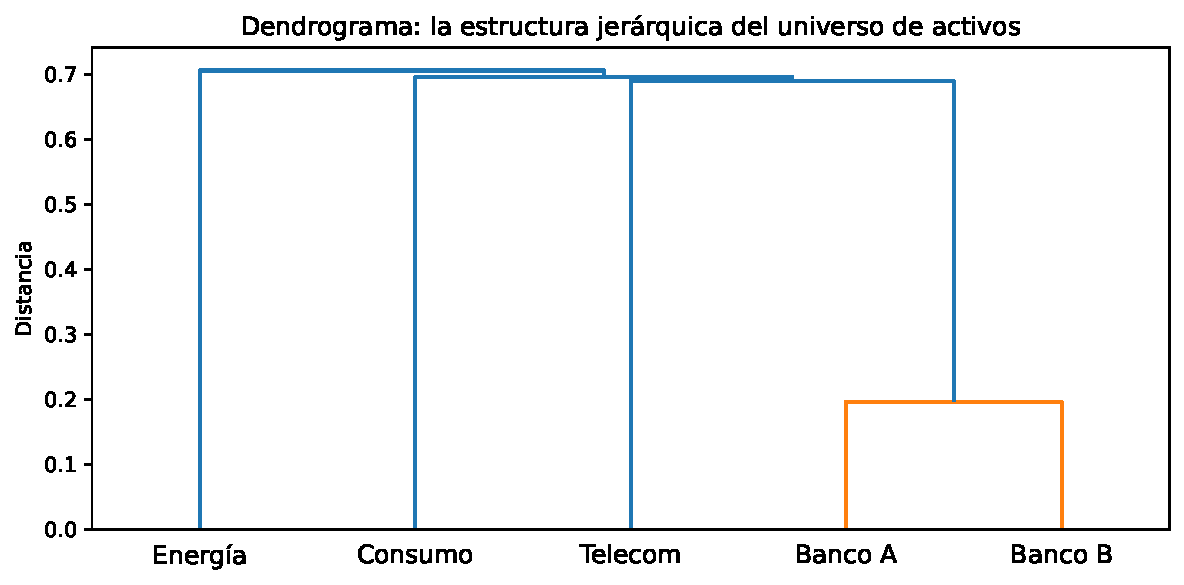
\includegraphics[keepaspectratio]{unidad2/cap09_hrp_files/figure-pdf/clustering-output-2.pdf}}

El dendrograma cuenta la historia que el optimizador de Markowitz nunca
ve: los dos bancos forman un grupo compacto (distancia chica), y recién
después se conectan con el resto. HRP va a usar exactamente esa
estructura.

\begin{center}\rule{0.5\linewidth}{0.5pt}\end{center}

\chapter{Paso 2: Quasi-diagonalización --- reordenar la
matriz}\label{paso-2-quasi-diagonalizaciuxf3n-reordenar-la-matriz}

El segundo paso es puramente organizativo: \textbf{reordenar los activos
según el orden de las hojas del árbol}, de modo que los activos
similares queden contiguos. Con ese orden, la matriz de covarianzas
queda ``casi diagonal por bloques'': las covarianzas grandes se
concentran cerca de la diagonal.

\begin{Shaded}
\begin{Highlighting}[]
\CommentTok{\# El orden de las hojas del dendrograma}
\NormalTok{orden }\OperatorTok{=}\NormalTok{ hierarchy.leaves\_list(enlaces)}
\NormalTok{tickers\_ordenados }\OperatorTok{=}\NormalTok{ corr.columns[orden].tolist()}
\BuiltInTok{print}\NormalTok{(}\StringTok{"Orden jerárquico:"}\NormalTok{, tickers\_ordenados)}

\CommentTok{\# Reordenamos la matriz de correlaciones con ese orden}
\NormalTok{corr\_ordenada }\OperatorTok{=}\NormalTok{ corr.iloc[orden, orden]}

\NormalTok{fig, axes }\OperatorTok{=}\NormalTok{ plt.subplots(}\DecValTok{1}\NormalTok{, }\DecValTok{2}\NormalTok{, figsize}\OperatorTok{=}\NormalTok{(}\DecValTok{10}\NormalTok{, }\DecValTok{4}\NormalTok{))}
\ControlFlowTok{for}\NormalTok{ ax, m, titulo }\KeywordTok{in}\NormalTok{ [(axes[}\DecValTok{0}\NormalTok{], corr, }\StringTok{"Original"}\NormalTok{),}
\NormalTok{                      (axes[}\DecValTok{1}\NormalTok{], corr\_ordenada, }\StringTok{"Quasi{-}diagonalizada"}\NormalTok{)]:}
\NormalTok{    im }\OperatorTok{=}\NormalTok{ ax.imshow(m, cmap}\OperatorTok{=}\StringTok{"coolwarm"}\NormalTok{, vmin}\OperatorTok{={-}}\DecValTok{1}\NormalTok{, vmax}\OperatorTok{=}\DecValTok{1}\NormalTok{)}
\NormalTok{    ax.set\_xticks(}\BuiltInTok{range}\NormalTok{(}\BuiltInTok{len}\NormalTok{(m)), m.columns, rotation}\OperatorTok{=}\DecValTok{45}\NormalTok{, ha}\OperatorTok{=}\StringTok{"right"}\NormalTok{)}
\NormalTok{    ax.set\_yticks(}\BuiltInTok{range}\NormalTok{(}\BuiltInTok{len}\NormalTok{(m)), m.columns)}
\NormalTok{    ax.set\_title(titulo)}
\NormalTok{fig.colorbar(im, ax}\OperatorTok{=}\NormalTok{axes, shrink}\OperatorTok{=}\FloatTok{0.8}\NormalTok{, label}\OperatorTok{=}\StringTok{"Correlación"}\NormalTok{)}
\NormalTok{plt.show()}
\end{Highlighting}
\end{Shaded}

\begin{verbatim}
Orden jerárquico: ['Energía', 'Consumo', 'Telecom', 'Banco A', 'Banco B']
\end{verbatim}

\pandocbounded{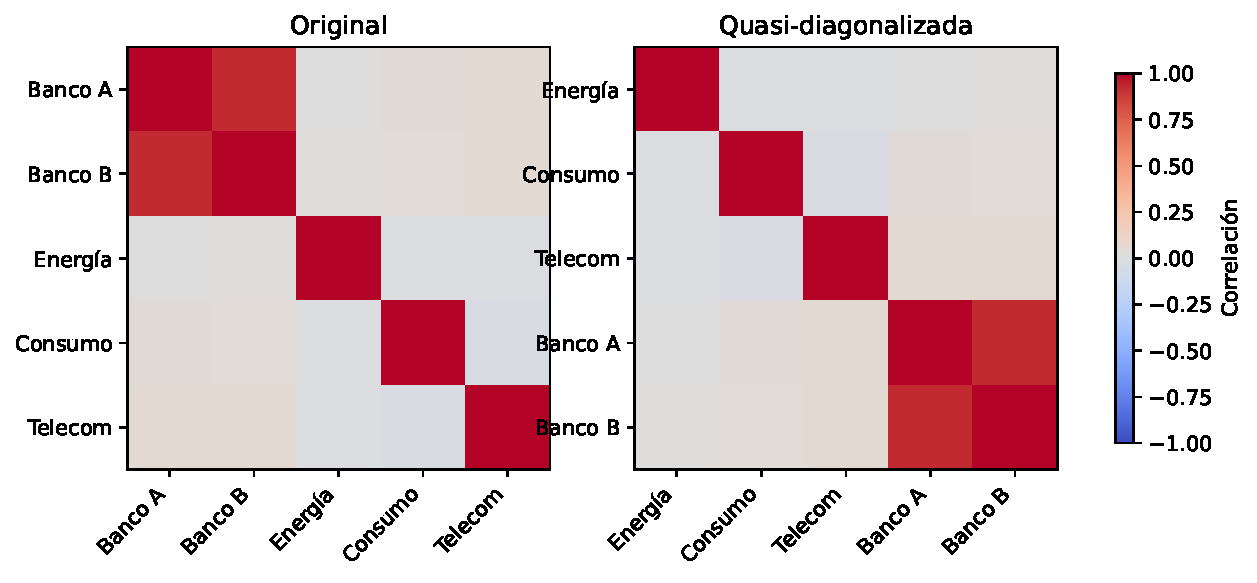
\includegraphics[keepaspectratio]{unidad2/cap09_hrp_files/figure-pdf/quasi-diag-output-2.pdf}}

En este ejemplo chico el reordenamiento es sutil, pero con decenas de
activos el efecto es dramático: los bloques de color (sectores,
regiones) se vuelven visibles a simple vista. La matriz reordenada es el
``mapa'' sobre el que repartiremos el capital.

\begin{center}\rule{0.5\linewidth}{0.5pt}\end{center}

\chapter{Paso 3: Recursive bisection --- repartir el capital por el
árbol}\label{paso-3-recursive-bisection-repartir-el-capital-por-el-uxe1rbol}

Acá está el corazón de HRP. En lugar de resolver un sistema global (que
exigiría invertir \(\Sigma\)), repartimos el capital \textbf{de arriba
hacia abajo}:

\begin{enumerate}
\def\labelenumi{\arabic{enumi}.}
\tightlist
\item
  Arrancamos con el 100\% del capital y la lista completa (ya ordenada)
  de activos.
\item
  Partimos la lista en dos mitades y calculamos el \textbf{riesgo de
  cada mitad}.
\item
  Le damos más capital a la mitad \textbf{menos riesgosa}, en proporción
  inversa a su varianza:
  \[\alpha_1 = 1 - \frac{V_1}{V_1 + V_2}, \qquad \alpha_2 = 1 - \alpha_1\]
\item
  Repetimos recursivamente dentro de cada mitad, hasta llegar a activos
  individuales.
\end{enumerate}

Para medir el riesgo de un grupo usamos la cartera
\emph{inverse-variance} dentro del grupo (cada activo pesa lo inverso de
su varianza), que tiene forma cerrada y \textbf{solo usa la diagonal}
---nada de inversas de matrices completas.

\phantomsection\label{hrp-implementacion}
\begin{Shaded}
\begin{Highlighting}[]
\KeywordTok{def}\NormalTok{ pesos\_inverse\_variance(cov):}
    \CommentTok{"""Pesos proporcionales a 1/varianza (solo usa la diagonal)."""}
\NormalTok{    iv }\OperatorTok{=} \DecValTok{1} \OperatorTok{/}\NormalTok{ np.diag(cov.values)}
    \ControlFlowTok{return}\NormalTok{ iv }\OperatorTok{/}\NormalTok{ iv.}\BuiltInTok{sum}\NormalTok{()}

\KeywordTok{def}\NormalTok{ varianza\_cluster(cov, items):}
    \CommentTok{"""Varianza del sub{-}portafolio inverse{-}variance de un grupo de activos."""}
\NormalTok{    sub }\OperatorTok{=}\NormalTok{ cov.loc[items, items]}
\NormalTok{    w }\OperatorTok{=}\NormalTok{ pesos\_inverse\_variance(sub)}
    \ControlFlowTok{return} \BuiltInTok{float}\NormalTok{(w }\OperatorTok{@}\NormalTok{ sub.values }\OperatorTok{@}\NormalTok{ w)}

\KeywordTok{def}\NormalTok{ hrp(cov, orden\_tickers):}
    \CommentTok{"""Recursive bisection sobre la lista ordenada de activos."""}
\NormalTok{    pesos }\OperatorTok{=}\NormalTok{ pd.Series(}\FloatTok{1.0}\NormalTok{, index}\OperatorTok{=}\NormalTok{orden\_tickers)}
\NormalTok{    grupos }\OperatorTok{=}\NormalTok{ [orden\_tickers]                      }\CommentTok{\# arrancamos con un solo grupo: todos}

    \ControlFlowTok{while}\NormalTok{ grupos:}
        \CommentTok{\# Partimos cada grupo vigente en dos mitades}
\NormalTok{        nuevos }\OperatorTok{=}\NormalTok{ []}
        \ControlFlowTok{for}\NormalTok{ g }\KeywordTok{in}\NormalTok{ grupos:}
            \ControlFlowTok{if} \BuiltInTok{len}\NormalTok{(g) }\OperatorTok{\textless{}=} \DecValTok{1}\NormalTok{:}
                \ControlFlowTok{continue}
\NormalTok{            mitad }\OperatorTok{=} \BuiltInTok{len}\NormalTok{(g) }\OperatorTok{//} \DecValTok{2}
\NormalTok{            izq, der }\OperatorTok{=}\NormalTok{ g[:mitad], g[mitad:]}

            \CommentTok{\# Riesgo de cada mitad y factor de asignación}
\NormalTok{            v\_izq }\OperatorTok{=}\NormalTok{ varianza\_cluster(cov, izq)}
\NormalTok{            v\_der }\OperatorTok{=}\NormalTok{ varianza\_cluster(cov, der)}
\NormalTok{            alpha }\OperatorTok{=} \DecValTok{1} \OperatorTok{{-}}\NormalTok{ v\_izq }\OperatorTok{/}\NormalTok{ (v\_izq }\OperatorTok{+}\NormalTok{ v\_der)}

\NormalTok{            pesos[izq] }\OperatorTok{*=}\NormalTok{ alpha        }\CommentTok{\# la mitad menos riesgosa recibe más capital}
\NormalTok{            pesos[der] }\OperatorTok{*=}\NormalTok{ (}\DecValTok{1} \OperatorTok{{-}}\NormalTok{ alpha)}

\NormalTok{            nuevos }\OperatorTok{+=}\NormalTok{ [izq, der]}
\NormalTok{        grupos }\OperatorTok{=}\NormalTok{ nuevos}

    \ControlFlowTok{return}\NormalTok{ pesos}

\NormalTok{cov }\OperatorTok{=}\NormalTok{ retornos.cov()}
\NormalTok{w\_hrp }\OperatorTok{=}\NormalTok{ hrp(cov, tickers\_ordenados)}

\BuiltInTok{print}\NormalTok{(}\StringTok{"Pesos HRP:"}\NormalTok{)}
\BuiltInTok{print}\NormalTok{((w\_hrp }\OperatorTok{*} \DecValTok{100}\NormalTok{).}\BuiltInTok{round}\NormalTok{(}\DecValTok{1}\NormalTok{).astype(}\BuiltInTok{str}\NormalTok{) }\OperatorTok{+} \StringTok{" \%"}\NormalTok{)}
\BuiltInTok{print}\NormalTok{(}\SpecialStringTok{f"}\CharTok{\textbackslash{}n}\SpecialStringTok{Suma: }\SpecialCharTok{\{}\NormalTok{w\_hrp}\SpecialCharTok{.}\BuiltInTok{sum}\NormalTok{()}\SpecialCharTok{:.1\%\}}\SpecialStringTok{"}\NormalTok{)}
\end{Highlighting}
\end{Shaded}

\begin{verbatim}
Pesos HRP:
Energía    20.8 %
Consumo    29.0 %
Telecom    38.4 %
Banco A     5.9 %
Banco B     5.9 %
dtype: str

Suma: 100.0%
\end{verbatim}

Observá el resultado: los dos bancos ---que comparten casi todo su
riesgo--- \textbf{se reparten entre sí la porción del capital que le
toca a su grupo}, en lugar de recibir cada uno una apuesta
independiente. Los activos diversificadores reciben pesos sustanciales y
\textbf{no aparece ninguna posición corta ni extrema}. Y en todo el
proceso no invertimos una sola matriz.

\begin{tcolorbox}[enhanced jigsaw, bottomrule=.15mm, colback=white, opacitybacktitle=0.6, arc=.35mm, toprule=.15mm, opacityback=0, breakable, titlerule=0mm, left=2mm, coltitle=black, colbacktitle=quarto-callout-tip-color!10!white, colframe=quarto-callout-tip-color-frame, leftrule=.75mm, toptitle=1mm, bottomtitle=1mm, title=\textcolor{quarto-callout-tip-color}{\faLightbulb}\hspace{0.5em}{Por qué esto es `risk parity' jerárquico}, rightrule=.15mm]

En cada bifurcación, el capital se reparte de manera inversamente
proporcional al riesgo: las dos ramas quedan aportando riesgos
comparables. Es la idea de \emph{risk parity} (paridad de riesgo),
aplicada recursivamente sobre la jerarquía del árbol en lugar de activo
por activo.

\end{tcolorbox}

\begin{center}\rule{0.5\linewidth}{0.5pt}\end{center}

\chapter{HRP vs.~Markowitz: la prueba fuera de
muestra}\label{hrp-vs.-markowitz-la-prueba-fuera-de-muestra}

La comparación justa no es ``qué cartera se ve mejor'' sino \textbf{cuál
funciona con datos que no vio}. Repetimos muchas veces el experimento:
estimamos ambas carteras con un período de entrenamiento y medimos su
volatilidad en el período siguiente.

\phantomsection\label{comparacion-oos}
\begin{Shaded}
\begin{Highlighting}[]
\KeywordTok{def}\NormalTok{ experimento(n\_sims}\OperatorTok{=}\DecValTok{200}\NormalTok{, n\_train}\OperatorTok{=}\DecValTok{250}\NormalTok{, n\_test}\OperatorTok{=}\DecValTok{250}\NormalTok{):}
\NormalTok{    vol\_mkw, vol\_hrp }\OperatorTok{=}\NormalTok{ [], []}

    \ControlFlowTok{for}\NormalTok{ sim }\KeywordTok{in} \BuiltInTok{range}\NormalTok{(n\_sims):}
\NormalTok{        r }\OperatorTok{=}\NormalTok{ simular\_retornos(n\_train }\OperatorTok{+}\NormalTok{ n\_test, seed}\OperatorTok{=}\DecValTok{1000} \OperatorTok{+}\NormalTok{ sim)}
\NormalTok{        train, test }\OperatorTok{=}\NormalTok{ r[:n\_train], r[n\_train:]}

\NormalTok{        df\_train }\OperatorTok{=}\NormalTok{ pd.DataFrame(train, columns}\OperatorTok{=}\NormalTok{corr.columns)}
\NormalTok{        cov\_train }\OperatorTok{=}\NormalTok{ df\_train.cov()}

        \CommentTok{\# {-}{-}{-} Markowitz: mínima varianza (requiere invertir Σ) {-}{-}{-}}
\NormalTok{        w\_m }\OperatorTok{=}\NormalTok{ pesos\_min\_varianza(cov\_train.values)}

        \CommentTok{\# {-}{-}{-} HRP: clustering + bisección (sin inversas) {-}{-}{-}}
\NormalTok{        d }\OperatorTok{=}\NormalTok{ np.sqrt((}\DecValTok{1} \OperatorTok{{-}}\NormalTok{ df\_train.corr()) }\OperatorTok{/} \DecValTok{2}\NormalTok{)}
\NormalTok{        lk }\OperatorTok{=}\NormalTok{ hierarchy.linkage(squareform(d.values), method}\OperatorTok{=}\StringTok{"single"}\NormalTok{)}
\NormalTok{        orden\_t }\OperatorTok{=}\NormalTok{ df\_train.columns[hierarchy.leaves\_list(lk)].tolist()}
\NormalTok{        w\_h }\OperatorTok{=}\NormalTok{ hrp(cov\_train, orden\_t).reindex(df\_train.columns).values}

        \CommentTok{\# Volatilidad realizada FUERA de muestra (anualizada)}
\NormalTok{        vol\_mkw.append(np.std(test }\OperatorTok{@}\NormalTok{ w\_m) }\OperatorTok{*}\NormalTok{ np.sqrt(}\DecValTok{252}\NormalTok{))}
\NormalTok{        vol\_hrp.append(np.std(test }\OperatorTok{@}\NormalTok{ w\_h) }\OperatorTok{*}\NormalTok{ np.sqrt(}\DecValTok{252}\NormalTok{))}

    \ControlFlowTok{return}\NormalTok{ np.array(vol\_mkw), np.array(vol\_hrp)}

\NormalTok{vol\_mkw, vol\_hrp }\OperatorTok{=}\NormalTok{ experimento()}

\BuiltInTok{print}\NormalTok{(}\StringTok{"Volatilidad anualizada fuera de muestra (promedio de 200 simulaciones):"}\NormalTok{)}
\BuiltInTok{print}\NormalTok{(}\SpecialStringTok{f"  Markowitz (mín. varianza): }\SpecialCharTok{\{}\NormalTok{vol\_mkw}\SpecialCharTok{.}\NormalTok{mean()}\SpecialCharTok{:.2\%\}}\SpecialStringTok{  (desvío entre sims: }\SpecialCharTok{\{}\NormalTok{vol\_mkw}\SpecialCharTok{.}\NormalTok{std()}\SpecialCharTok{:.2\%\}}\SpecialStringTok{)"}\NormalTok{)}
\BuiltInTok{print}\NormalTok{(}\SpecialStringTok{f"  HRP:                       }\SpecialCharTok{\{}\NormalTok{vol\_hrp}\SpecialCharTok{.}\NormalTok{mean()}\SpecialCharTok{:.2\%\}}\SpecialStringTok{  (desvío entre sims: }\SpecialCharTok{\{}\NormalTok{vol\_hrp}\SpecialCharTok{.}\NormalTok{std()}\SpecialCharTok{:.2\%\}}\SpecialStringTok{)"}\NormalTok{)}
\end{Highlighting}
\end{Shaded}

\begin{verbatim}
Volatilidad anualizada fuera de muestra (promedio de 200 simulaciones):
  Markowitz (mín. varianza): 8.31%  (desvío entre sims: 0.38%)
  HRP:                       8.39%  (desvío entre sims: 0.42%)
\end{verbatim}

\begin{Shaded}
\begin{Highlighting}[]
\NormalTok{fig, ax }\OperatorTok{=}\NormalTok{ plt.subplots(figsize}\OperatorTok{=}\NormalTok{(}\DecValTok{9}\NormalTok{, }\DecValTok{4}\NormalTok{))}
\NormalTok{ax.hist(vol\_mkw }\OperatorTok{*} \DecValTok{100}\NormalTok{, bins}\OperatorTok{=}\DecValTok{30}\NormalTok{, alpha}\OperatorTok{=}\FloatTok{0.6}\NormalTok{, label}\OperatorTok{=}\StringTok{"Markowitz (mín. varianza)"}\NormalTok{)}
\NormalTok{ax.hist(vol\_hrp }\OperatorTok{*} \DecValTok{100}\NormalTok{, bins}\OperatorTok{=}\DecValTok{30}\NormalTok{, alpha}\OperatorTok{=}\FloatTok{0.6}\NormalTok{, label}\OperatorTok{=}\StringTok{"HRP"}\NormalTok{)}
\NormalTok{ax.set\_xlabel(}\StringTok{"Volatilidad anualizada fuera de muestra (\%)"}\NormalTok{)}
\NormalTok{ax.set\_ylabel(}\StringTok{"Frecuencia"}\NormalTok{)}
\NormalTok{ax.set\_title(}\StringTok{"Riesgo realizado fuera de muestra: 200 simulaciones"}\NormalTok{)}
\NormalTok{ax.legend()}
\NormalTok{ax.grid(}\VariableTok{True}\NormalTok{, alpha}\OperatorTok{=}\FloatTok{0.3}\NormalTok{)}
\NormalTok{plt.tight\_layout()}
\NormalTok{plt.show()}
\end{Highlighting}
\end{Shaded}

\pandocbounded{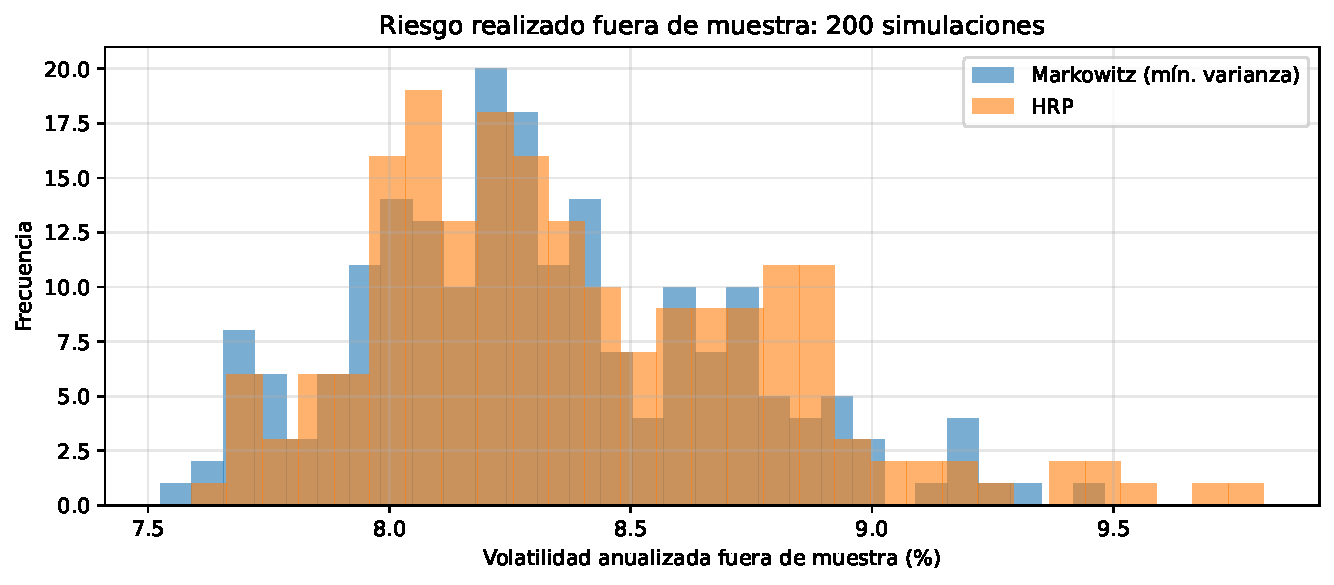
\includegraphics[keepaspectratio]{unidad2/cap09_hrp_files/figure-pdf/comparacion-grafico-output-1.pdf}}

El patrón típico (y el que reporta el paper original): dentro de la
muestra Markowitz siempre ``gana'' ---por definición minimiza la
varianza \emph{de esos datos}---, pero \textbf{fuera de muestra HRP es
más estable y frecuentemente más eficiente}, porque no gastó grados de
libertad ajustándose al ruido. La distribución de HRP suele ser más
angosta: menos sorpresas.

\begin{tcolorbox}[enhanced jigsaw, bottomrule=.15mm, colback=white, opacitybacktitle=0.6, arc=.35mm, toprule=.15mm, opacityback=0, breakable, titlerule=0mm, left=2mm, coltitle=black, colbacktitle=quarto-callout-warning-color!10!white, colframe=quarto-callout-warning-color-frame, leftrule=.75mm, toptitle=1mm, bottomtitle=1mm, title=\textcolor{quarto-callout-warning-color}{\faExclamationTriangle}\hspace{0.5em}{HRP no es magia}, rightrule=.15mm]

HRP renuncia a usar información que Markowitz sí usa (las correlaciones
exactas entre grupos lejanos y los retornos esperados). Si tus
estimaciones de \(\mu\) y \(\Sigma\) fueran perfectas, Markowitz sería
imbatible. HRP gana justamente porque en el mundo real \textbf{nunca lo
son}. La elección depende de cuánto confiás en tus estimaciones --- un
tema que retomamos en el capítulo siguiente con Black-Litterman, que
ataca el mismo problema desde otro ángulo: mejorar las estimaciones en
lugar de esquivarlas.

\end{tcolorbox}

\begin{center}\rule{0.5\linewidth}{0.5pt}\end{center}

\chapter{Con datos reales}\label{con-datos-reales-1}

La simulación nos dejó controlar la estructura de correlaciones; ahora
veamos si HRP la \textbf{descubre solo} en datos de mercado. Usamos el
dataset del libro (\texttt{datos/precios.csv}, ver
Apéndice~\ref{sec-datos-financieros}): 9 acciones de sectores distintos,
cinco años de precios diarios ajustados.

\begin{Shaded}
\begin{Highlighting}[]
\NormalTok{precios }\OperatorTok{=}\NormalTok{ pd.read\_csv(}\StringTok{"../datos/precios.csv"}\NormalTok{, index\_col}\OperatorTok{=}\StringTok{"Date"}\NormalTok{, parse\_dates}\OperatorTok{=}\VariableTok{True}\NormalTok{)}
\NormalTok{r\_real }\OperatorTok{=}\NormalTok{ precios.drop(columns}\OperatorTok{=}\StringTok{"SPY"}\NormalTok{).pct\_change().dropna()   }\CommentTok{\# SPY es un índice, no un activo más}

\CommentTok{\# El pipeline completo de HRP, tal cual lo construimos}
\NormalTok{dist\_real }\OperatorTok{=}\NormalTok{ np.sqrt((}\DecValTok{1} \OperatorTok{{-}}\NormalTok{ r\_real.corr()) }\OperatorTok{/} \DecValTok{2}\NormalTok{)}
\NormalTok{enlaces\_real }\OperatorTok{=}\NormalTok{ hierarchy.linkage(squareform(dist\_real.values), method}\OperatorTok{=}\StringTok{"single"}\NormalTok{)}

\NormalTok{fig, ax }\OperatorTok{=}\NormalTok{ plt.subplots(figsize}\OperatorTok{=}\NormalTok{(}\DecValTok{9}\NormalTok{, }\DecValTok{4}\NormalTok{))}
\NormalTok{hierarchy.dendrogram(enlaces\_real, labels}\OperatorTok{=}\NormalTok{r\_real.columns.tolist(), ax}\OperatorTok{=}\NormalTok{ax)}
\NormalTok{ax.set\_title(}\StringTok{"Dendrograma de 9 acciones reales (2021–2026)"}\NormalTok{)}
\NormalTok{ax.set\_ylabel(}\StringTok{"Distancia"}\NormalTok{)}
\NormalTok{plt.tight\_layout()}
\NormalTok{plt.show()}
\end{Highlighting}
\end{Shaded}

\pandocbounded{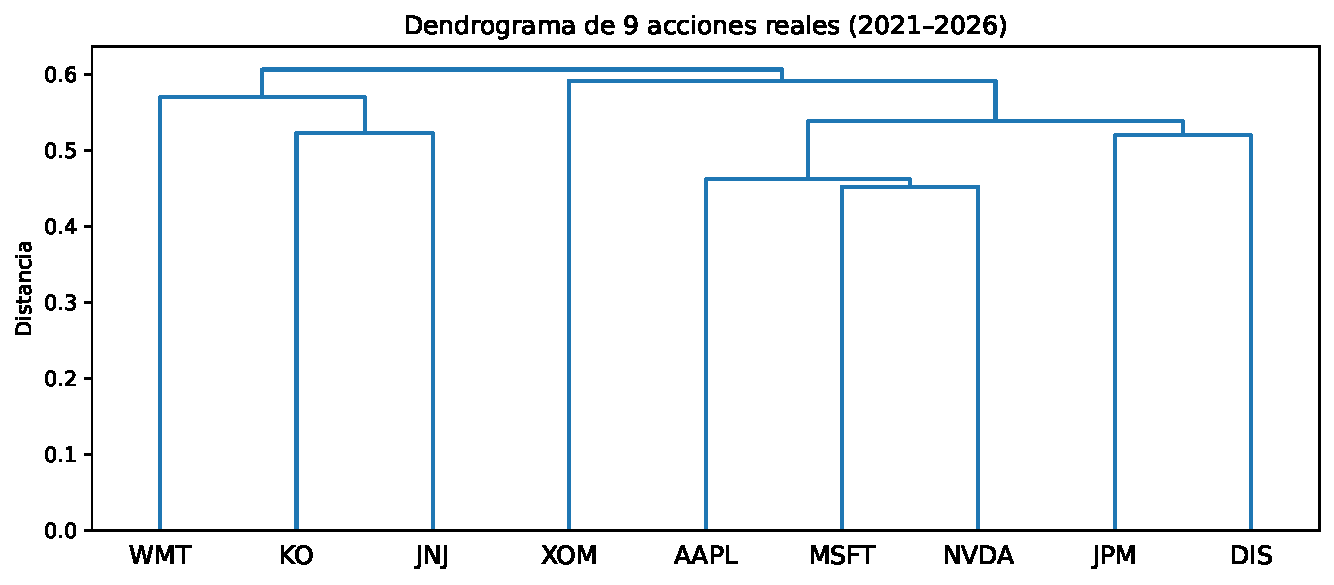
\includegraphics[keepaspectratio]{unidad2/cap09_hrp_files/figure-pdf/hrp-datos-reales-output-1.pdf}}

Mirá el dendrograma antes de seguir: \textbf{nadie le dijo al algoritmo
qué sector es cada empresa}, y sin embargo las tecnológicas (AAPL, MSFT,
NVDA) se abrazan en un cluster compacto, y las defensivas de consumo
(KO, JNJ, WMT) forman el suyo. La estructura jerárquica que López de
Prado postula no es una hipótesis: está en los datos.

\phantomsection\label{hrp-pesos-reales}
\begin{Shaded}
\begin{Highlighting}[]
\NormalTok{orden\_real }\OperatorTok{=}\NormalTok{ r\_real.columns[hierarchy.leaves\_list(enlaces\_real)].tolist()}
\NormalTok{w\_hrp\_real }\OperatorTok{=}\NormalTok{ hrp(r\_real.cov(), orden\_real)}
\NormalTok{w\_mkw\_real }\OperatorTok{=}\NormalTok{ pd.Series(pesos\_min\_varianza(r\_real.cov().values), index}\OperatorTok{=}\NormalTok{r\_real.columns)}

\NormalTok{comparacion }\OperatorTok{=}\NormalTok{ pd.DataFrame(\{}\StringTok{"HRP"}\NormalTok{: w\_hrp\_real, }\StringTok{"Markowitz mín. var."}\NormalTok{: w\_mkw\_real\})}
\BuiltInTok{print}\NormalTok{((comparacion }\OperatorTok{*} \DecValTok{100}\NormalTok{).}\BuiltInTok{round}\NormalTok{(}\DecValTok{1}\NormalTok{).astype(}\BuiltInTok{str}\NormalTok{) }\OperatorTok{+} \StringTok{" \%"}\NormalTok{)}
\end{Highlighting}
\end{Shaded}

\begin{verbatim}
         HRP Markowitz mín. var.
AAPL   6.3 %              -3.5 %
DIS    4.9 %               1.6 %
JNJ   25.5 %              30.4 %
JPM    7.1 %               6.0 %
KO    23.6 %              27.9 %
MSFT   6.6 %              12.6 %
NVDA   2.3 %               1.5 %
WMT   13.2 %              12.1 %
XOM   10.5 %              11.6 %
\end{verbatim}

La comparación repite lo que vimos en la simulación, ahora sin trucos.
Buscá en la columna de Markowitz las tecnológicas: \textbf{shortea una
para comprar otra} --- la apuesta fina entre ``gemelos'' que en el
experimento sintético identificamos como puro ruido muestral,
reproducida con datos de verdad. Con 9 activos el daño es contenido; con
50 o 100, esos cortos se multiplican. HRP, en cambio, asigna a
\textbf{todos} los activos pesos positivos y moderados, dándole más
capital al cluster defensivo y repartiendo dentro de cada grupo. Es la
cartera que podrías ejecutar mañana sin explicarle nada raro a un comité
de inversiones.

\begin{center}\rule{0.5\linewidth}{0.5pt}\end{center}

\chapter{Errores comunes}\label{errores-comunes-7}

\begin{tcolorbox}[enhanced jigsaw, bottomrule=.15mm, colback=white, opacitybacktitle=0.6, arc=.35mm, toprule=.15mm, opacityback=0, breakable, titlerule=0mm, left=2mm, coltitle=black, colbacktitle=quarto-callout-warning-color!10!white, colframe=quarto-callout-warning-color-frame, leftrule=.75mm, toptitle=1mm, bottomtitle=1mm, title=\textcolor{quarto-callout-warning-color}{\faExclamationTriangle}\hspace{0.5em}{Trampas frecuentes}, rightrule=.15mm]

\begin{itemize}
\tightlist
\item
  \textbf{Pasarle a \texttt{linkage} la matriz cuadrada directamente}:
  \texttt{scipy} espera la forma \emph{condensada} (vector triangular);
  usá \texttt{squareform(dist)} o interpretará las filas como
  observaciones.
\item
  \textbf{Olvidar reordenar antes de la bisección}: la partición en
  mitades solo tiene sentido sobre la lista quasi-diagonalizada. Sobre
  el orden original, las mitades mezclan grupos y HRP pierde su lógica.
\item
  \textbf{Usar la correlación como distancia sin transformar}: la
  correlación no es una métrica (activos idénticos tendrían
  ``distancia'' 1). La transformación \(\sqrt{(1-\rho)/2}\) es la que
  convierte similitud en distancia válida.
\item
  \textbf{Comparar métodos dentro de la muestra}: cualquier optimizador
  le gana a HRP con los datos con los que fue ajustado. La comparación
  honesta es siempre fuera de muestra.
\end{itemize}

\end{tcolorbox}

\begin{center}\rule{0.5\linewidth}{0.5pt}\end{center}

\chapter{Ejercicios Propuestos}\label{ejercicios-propuestos-8}

\begin{tcolorbox}[enhanced jigsaw, bottomrule=.15mm, colback=white, opacitybacktitle=0.6, arc=.35mm, toprule=.15mm, opacityback=0, breakable, titlerule=0mm, left=2mm, coltitle=black, colbacktitle=quarto-callout-important-color!10!white, colframe=quarto-callout-important-color-frame, leftrule=.75mm, toptitle=1mm, bottomtitle=1mm, title=\textcolor{quarto-callout-important-color}{\faExclamation}\hspace{0.5em}{Ejercicios}, rightrule=.15mm]

\begin{enumerate}
\def\labelenumi{\arabic{enumi}.}
\tightlist
\item
  \textbf{Sensibilidad al linkage}: repetí el clustering con
  \texttt{method="ward"} y \texttt{method="complete"}. ¿Cambia el orden
  de las hojas? ¿Y los pesos finales?
\item
  \textbf{Más activos}: extendé la simulación a 10 activos con 3 grupos
  de correlación y verificá que los bloques aparecen en la matriz
  quasi-diagonalizada.
\item
  \textbf{Equiponderada como referencia}: agregá al experimento fuera de
  muestra la cartera equiponderada (\(w_i = 1/N\)). ¿Dónde queda
  respecto de Markowitz y HRP?
\item
  \textbf{Estrés de correlación}: aumentá la correlación de los
  ``gemelos'' a 0.99 y observá qué pasa con los pesos de Markowitz y con
  los de HRP.
\item
  \textbf{HRP con otro linkage sobre datos reales}: repetí la sección
  ``Con datos reales'' usando \texttt{method="ward"} en lugar de
  \texttt{single}. ¿Cambian los clusters? ¿Y los pesos? ¿Cuál te resulta
  más creíble económicamente?
\end{enumerate}

\end{tcolorbox}

Podés resolver estos ejercicios acá mismo: la celda ejecuta Python
\textbf{en tu navegador}, sin instalar nada (la primera ejecución tarda
unos segundos mientras carga el entorno; los paquetes que importes se
instalan solos).

\begin{Shaded}
\begin{Highlighting}[]
\NormalTok{\#| label: practica{-}navegador}
\NormalTok{import numpy as np}
\NormalTok{import pandas as pd}
\NormalTok{from scipy.cluster import hierarchy}
\NormalTok{from scipy.spatial.distance import squareform}

\NormalTok{\# Para usar el dataset real del libro (requiere conexión):}
\NormalTok{\# import pandas as pd}
\NormalTok{\# from pyodide.http import open\_url}
\NormalTok{\# url = "https://diegoonna.github.io/libro\_finanzas\_computacionales/datos/precios.csv"}
\NormalTok{\# precios = pd.read\_csv(open\_url(url), index\_col="Date", parse\_dates=True)}

\NormalTok{\# Tu solución acá...}
\end{Highlighting}
\end{Shaded}

\begin{center}\rule{0.5\linewidth}{0.5pt}\end{center}

\chapter{Referencias}\label{referencias-8}

\phantomsection\label{refs}

\chapter{Capítulo 10: El Modelo de
Black-Litterman}\label{capuxedtulo-10-el-modelo-de-black-litterman}

Del equilibrio de mercado a las views del inversor (enfoque algebraico)

Markowitz tiene un problema práctico: es hipersensible a los retornos
esperados que le pasamos, y esos retornos son justamente lo más difícil
de estimar. Black y Litterman lo resolvieron con una idea elegante:
partir del retorno que el propio mercado está implícitamente asumiendo
(el equilibrio) y ajustarlo solo donde el inversor tiene una opinión
fundada. En este capítulo lo derivamos por el método clásico y
algebraico, paso a paso.

\hfill\break

\chapter{Introducción: por qué Markowitz solo no
alcanza}\label{introducciuxf3n-por-quuxe9-markowitz-solo-no-alcanza}

En el Capítulo 8 aprendimos a construir la frontera eficiente. Pero si
intentás usar Markowitz ``puro'' con datos reales, te chocás con un
problema incómodo: \textbf{el modelo es extremadamente sensible a los
retornos esperados} \(\boldsymbol{\mu}\) que le das de entrada. Cambiás
la estimación del retorno de un activo en medio punto y la cartera
óptima se da vuelta por completo, concentrándose en dos o tres
posiciones extremas (a veces con ventas en corto gigantes).

El problema de fondo es que \(\boldsymbol{\mu}\) es lo más difícil de
estimar en finanzas: el promedio histórico es un estimador malísimo del
retorno futuro. Entonces alimentamos el modelo más sensible con el input
más ruidoso. El resultado son carteras que ningún gestor firmaría.

\textbf{Black-Litterman} (1992), nacido en Goldman Sachs, ataca el
problema con un cambio de perspectiva:

\begin{quote}
En lugar de \emph{inventar} los retornos esperados desde cero,
arranquemos del retorno que el mercado ya está asumiendo hoy, y
ajustémoslo solo donde tengamos una opinión concreta y en la medida de
nuestra confianza en ella.
\end{quote}

\begin{tcolorbox}[enhanced jigsaw, bottomrule=.15mm, colback=white, opacitybacktitle=0.6, arc=.35mm, toprule=.15mm, opacityback=0, breakable, titlerule=0mm, left=2mm, coltitle=black, colbacktitle=quarto-callout-tip-color!10!white, colframe=quarto-callout-tip-color-frame, leftrule=.75mm, toptitle=1mm, bottomtitle=1mm, title=\textcolor{quarto-callout-tip-color}{\faLightbulb}\hspace{0.5em}{La idea en una frase}, rightrule=.15mm]

Markowitz te pregunta \emph{``¿cuánto va a rendir cada activo?''} y se
cree tu respuesta al pie de la letra. Black-Litterman te pregunta
\emph{``¿en qué diferís del mercado, y cuán seguro estás?''} --- una
pregunta mucho más honesta y fácil de responder.

\end{tcolorbox}

\phantomsection\label{setup}
\begin{Shaded}
\begin{Highlighting}[]
\ImportTok{import}\NormalTok{ numpy }\ImportTok{as}\NormalTok{ np}
\NormalTok{np.set\_printoptions(precision}\OperatorTok{=}\DecValTok{4}\NormalTok{, suppress}\OperatorTok{=}\VariableTok{True}\NormalTok{)}
\end{Highlighting}
\end{Shaded}

\begin{center}\rule{0.5\linewidth}{0.5pt}\end{center}

\chapter{La intuición: combinar una creencia previa con nueva
información}\label{la-intuiciuxf3n-combinar-una-creencia-previa-con-nueva-informaciuxf3n}

Antes de la matemática, la intuición, porque es el corazón del modelo.

Imaginate que querés estimar cuánto va a rendir una acción. Tenés dos
fuentes de información:

\begin{enumerate}
\def\labelenumi{\arabic{enumi}.}
\tightlist
\item
  Una \textbf{creencia previa}: ``el mercado, con todo su peso, está
  descontando un 8\% para este activo''. Es una referencia sensata y
  difícil de discutir.
\item
  Una \textbf{opinión propia} (nueva información): ``yo estudié el
  sector y creo que va a rendir 12\%''.
\end{enumerate}

¿Con qué te quedás? Ni una ni otra a ciegas: hacés un \textbf{promedio
ponderado por tu confianza}. Si tu análisis es muy sólido, tu estimación
final se acerca al 12\%; si tenés dudas, se queda cerca del 8\% del
mercado. Y si tu opinión coincide con el mercado, no cambia nada.

Ese mecanismo ---partir de una creencia y moverla hacia la nueva
evidencia en proporción a la confianza--- es exactamente lo que
formaliza Black-Litterman. En la literatura vas a ver que la versión
completa se deriva como una actualización bayesiana (\emph{prior} +
verosimilitud → \emph{posterior}), pero \textbf{no hace falta la
maquinaria bayesiana} para entenderlo ni usarlo: se puede escribir como
un conjunto de operaciones matriciales cerradas. Ese es el camino que
vamos a tomar.

\begin{center}\rule{0.5\linewidth}{0.5pt}\end{center}

\chapter{Paso 1: los retornos implícitos de equilibrio (optimización
inversa)}\label{paso-1-los-retornos-impluxedcitos-de-equilibrio-optimizaciuxf3n-inversa}

La primera pieza es la creencia de partida: ¿cuáles son los retornos que
el mercado está asumiendo? Acá viene el truco más lindo del modelo.

En Markowitz, dada una matriz de covarianzas \(\Sigma\) y unos retornos
esperados \(\boldsymbol{\mu}\), buscamos los pesos óptimos
\(\mathbf{w}\). Black-Litterman \textbf{invierte esa lógica}: si
suponemos que la cartera de mercado (la capitalización de cada activo)
ya es óptima ---porque es el consenso agregado de todos los
inversores---, entonces podemos despejar qué retornos
\(\boldsymbol{\Pi}\) la harían óptima. Es \emph{optimización inversa}.

El resultado es la fórmula del retorno implícito de equilibrio:

\[\boldsymbol{\Pi} = \delta \, \Sigma \, \mathbf{w}_{mkt}\]

donde:

\begin{itemize}
\tightlist
\item
  \(\mathbf{w}_{mkt}\) son los pesos de la cartera de mercado (por
  capitalización),
\item
  \(\Sigma\) es la matriz de covarianzas de los retornos,
\item
  \(\delta\) es el \textbf{coeficiente de aversión al riesgo} del
  mercado (típicamente entre 2 y 3).
\end{itemize}

\phantomsection\label{equilibrio}
\begin{Shaded}
\begin{Highlighting}[]
\CommentTok{\# Universo de ejemplo: 3 activos (digamos, tres clases de activos)}
\NormalTok{activos }\OperatorTok{=}\NormalTok{ [}\StringTok{"Acciones USA"}\NormalTok{, }\StringTok{"Acciones EU"}\NormalTok{, }\StringTok{"Bonos"}\NormalTok{]}

\CommentTok{\# Pesos de mercado (por capitalización) — suman 1}
\NormalTok{w\_mkt }\OperatorTok{=}\NormalTok{ np.array([}\FloatTok{0.55}\NormalTok{, }\FloatTok{0.30}\NormalTok{, }\FloatTok{0.15}\NormalTok{])}

\CommentTok{\# Matriz de covarianzas anual de los retornos}
\NormalTok{Sigma }\OperatorTok{=}\NormalTok{ np.array([}
\NormalTok{    [}\FloatTok{0.0225}\NormalTok{, }\FloatTok{0.0075}\NormalTok{, }\FloatTok{0.0010}\NormalTok{],}
\NormalTok{    [}\FloatTok{0.0075}\NormalTok{, }\FloatTok{0.0196}\NormalTok{, }\FloatTok{0.0012}\NormalTok{],}
\NormalTok{    [}\FloatTok{0.0010}\NormalTok{, }\FloatTok{0.0012}\NormalTok{, }\FloatTok{0.0036}\NormalTok{],}
\NormalTok{])}

\CommentTok{\# Aversión al riesgo del mercado}
\NormalTok{delta }\OperatorTok{=} \FloatTok{2.5}

\CommentTok{\# Retornos implícitos de equilibrio: Π = δ Σ w\_mkt}
\NormalTok{Pi }\OperatorTok{=}\NormalTok{ delta }\OperatorTok{*}\NormalTok{ Sigma }\OperatorTok{@}\NormalTok{ w\_mkt}

\ControlFlowTok{for}\NormalTok{ a, pi }\KeywordTok{in} \BuiltInTok{zip}\NormalTok{(activos, Pi):}
    \BuiltInTok{print}\NormalTok{(}\SpecialStringTok{f"}\SpecialCharTok{\{}\NormalTok{a}\SpecialCharTok{:\textless{}14\}}\SpecialStringTok{ retorno implícito: }\SpecialCharTok{\{}\NormalTok{pi}\SpecialCharTok{:6.2\%\}}\SpecialStringTok{"}\NormalTok{)}
\end{Highlighting}
\end{Shaded}

\begin{verbatim}
Acciones USA   retorno implícito:  3.69%
Acciones EU    retorno implícito:  2.55%
Bonos          retorno implícito:  0.36%
\end{verbatim}

Fijate lo que acabamos de lograr: \textbf{sin estimar un solo retorno
esperado a mano}, obtuvimos un vector \(\boldsymbol{\Pi}\) razonable,
coherente con el riesgo de cada activo y con lo que el mercado
efectivamente tiene comprado. Los activos más riesgosos y con más peso
en el mercado tienen mayor retorno implícito. Este \(\boldsymbol{\Pi}\)
es nuestra creencia de partida.

\begin{tcolorbox}[enhanced jigsaw, bottomrule=.15mm, colback=white, opacitybacktitle=0.6, arc=.35mm, toprule=.15mm, opacityback=0, breakable, titlerule=0mm, left=2mm, coltitle=black, colbacktitle=quarto-callout-note-color!10!white, colframe=quarto-callout-note-color-frame, leftrule=.75mm, toptitle=1mm, bottomtitle=1mm, title=\textcolor{quarto-callout-note-color}{\faInfo}\hspace{0.5em}{¿De dónde sale δ?}, rightrule=.15mm]

El coeficiente de aversión al riesgo se puede estimar como
\(\delta = (\mu_{mkt} - r_f) / \sigma_{mkt}^2\): el premio por riesgo
del mercado dividido por su varianza. Con un premio del
\textasciitilde5\% y una volatilidad del \textasciitilde14\% anual, da
\(\delta \approx 2.5\), el valor que usamos.

\end{tcolorbox}

\begin{center}\rule{0.5\linewidth}{0.5pt}\end{center}

\chapter{Paso 2: expresar las views del
inversor}\label{paso-2-expresar-las-views-del-inversor}

Ahora incorporamos nuestras opiniones. Black-Litterman las representa
con tres objetos:

\begin{itemize}
\tightlist
\item
  \textbf{\(P\)} (matriz de \emph{picks}): qué activos involucra cada
  view. Cada fila es una view.
\item
  \textbf{\(Q\)} (vector): el retorno que afirma cada view.
\item
  \textbf{\(\Omega\)} (matriz): la \textbf{incertidumbre} de cada view
  (cuánto desconfiamos de ella). Diagonal, un valor por view.
\end{itemize}

Las views pueden ser de dos tipos:

\begin{itemize}
\tightlist
\item
  \textbf{Absolutas}: ``Acciones EU van a rendir 12\%''. La fila de
  \(P\) tiene un \texttt{1} en ese activo y \texttt{0} en el resto.
\item
  \textbf{Relativas}: ``Acciones USA van a superar a Bonos por 4\%''. La
  fila tiene un \texttt{+1} en USA y un \texttt{-1} en Bonos.
\end{itemize}

\phantomsection\label{views}
\begin{Shaded}
\begin{Highlighting}[]
\CommentTok{\# View 1 (absoluta): "Acciones EU rendirán 12\%"}
\CommentTok{\# View 2 (relativa): "Acciones USA superarán a Bonos por 4\%"}
\NormalTok{P }\OperatorTok{=}\NormalTok{ np.array([}
\NormalTok{    [}\FloatTok{0.0}\NormalTok{, }\FloatTok{1.0}\NormalTok{,  }\FloatTok{0.0}\NormalTok{],   }\CommentTok{\# EU}
\NormalTok{    [}\FloatTok{1.0}\NormalTok{, }\FloatTok{0.0}\NormalTok{, }\OperatorTok{{-}}\FloatTok{1.0}\NormalTok{],   }\CommentTok{\# USA {-} Bonos}
\NormalTok{])}

\NormalTok{Q }\OperatorTok{=}\NormalTok{ np.array([}\FloatTok{0.12}\NormalTok{, }\FloatTok{0.04}\NormalTok{])   }\CommentTok{\# retornos afirmados por cada view}

\BuiltInTok{print}\NormalTok{(}\StringTok{"Matriz P (picks):}\CharTok{\textbackslash{}n}\StringTok{"}\NormalTok{, P)}
\BuiltInTok{print}\NormalTok{(}\StringTok{"}\CharTok{\textbackslash{}n}\StringTok{Vector Q (views):"}\NormalTok{, Q)}
\end{Highlighting}
\end{Shaded}

\begin{verbatim}
Matriz P (picks):
 [[ 0.  1.  0.]
 [ 1.  0. -1.]]

Vector Q (views): [0.12 0.04]
\end{verbatim}

Para la incertidumbre \(\Omega\), una convención estándar (Idzorek) es
hacerla proporcional a la varianza de la propia view bajo el modelo:
views sobre activos más volátiles arrastran más incertidumbre. Aparece
también un parámetro escalar \(\tau\) (chico,
\textasciitilde0.025--0.05) que refleja la confianza global en el
equilibrio.

\phantomsection\label{omega}
\begin{Shaded}
\begin{Highlighting}[]
\NormalTok{tau }\OperatorTok{=} \FloatTok{0.05}   \CommentTok{\# escala de la incertidumbre del equilibrio}

\CommentTok{\# Ω diagonal, proporcional a la incertidumbre de cada view: diag(P (τΣ) Pᵀ)}
\NormalTok{Omega }\OperatorTok{=}\NormalTok{ np.diag(np.diag(P }\OperatorTok{@}\NormalTok{ (tau }\OperatorTok{*}\NormalTok{ Sigma) }\OperatorTok{@}\NormalTok{ P.T))}

\BuiltInTok{print}\NormalTok{(}\StringTok{"Matriz Ω (incertidumbre de las views):}\CharTok{\textbackslash{}n}\StringTok{"}\NormalTok{, Omega)}
\end{Highlighting}
\end{Shaded}

\begin{verbatim}
Matriz Ω (incertidumbre de las views):
 [[0.001  0.    ]
 [0.     0.0012]]
\end{verbatim}

\begin{tcolorbox}[enhanced jigsaw, bottomrule=.15mm, colback=white, opacitybacktitle=0.6, arc=.35mm, toprule=.15mm, opacityback=0, breakable, titlerule=0mm, left=2mm, coltitle=black, colbacktitle=quarto-callout-tip-color!10!white, colframe=quarto-callout-tip-color-frame, leftrule=.75mm, toptitle=1mm, bottomtitle=1mm, title=\textcolor{quarto-callout-tip-color}{\faLightbulb}\hspace{0.5em}{El sentido de Ω}, rightrule=.15mm]

\(\Omega\) es la perilla de confianza. Si ponés valores \textbf{chicos},
le estás diciendo al modelo ``estoy muy seguro de estas views'' y el
resultado se pegará a \(Q\). Si los ponés \textbf{grandes}, el modelo
casi las ignora y se queda con el equilibrio \(\Pi\). Es la traducción
matemática del ``cuán seguro estás'' de la introducción.

\end{tcolorbox}

\begin{center}\rule{0.5\linewidth}{0.5pt}\end{center}

\chapter{Paso 3: la fórmula maestra de
Black-Litterman}\label{paso-3-la-fuxf3rmula-maestra-de-black-litterman}

Con el equilibrio \(\boldsymbol{\Pi}\) y las views \((P, Q, \Omega)\),
combinamos ambas fuentes en un único vector de retornos esperados
ajustados, \(\boldsymbol{\mu}_{BL}\). Esta es la célebre \emph{fórmula
maestra}:

\[\boldsymbol{\mu}_{BL} = \left[ (\tau\Sigma)^{-1} + P^T \Omega^{-1} P \right]^{-1} \left[ (\tau\Sigma)^{-1} \boldsymbol{\Pi} + P^T \Omega^{-1} Q \right]\]

Parece intimidante, pero es exactamente el \textbf{promedio ponderado
por confianza} de la intuición, escrito en matrices. Cada término
\((\cdot)^{-1}\) es una ``precisión'' (lo inverso de la incertidumbre):
el equilibrio pesa según su precisión \((\tau\Sigma)^{-1}\) y las views
según la suya \(P^T\Omega^{-1}P\). Donde no hay view, prevalece el
equilibrio; donde hay una view muy confiable, ella domina.

Para verlo, conviene mirar el caso de \textbf{un solo activo con una
sola view}: la fórmula se reduce a

\[\mu_{BL} = \frac{\pi/\sigma_\pi^2 + q/\sigma_q^2}{1/\sigma_\pi^2 + 1/\sigma_q^2}\]

que es literalmente un promedio de \(\pi\) (equilibrio) y \(q\) (view)
ponderado por las precisiones. La versión matricial hace lo mismo con
todos los activos y views a la vez, respetando las correlaciones.

\phantomsection\label{formula-maestra}
\begin{Shaded}
\begin{Highlighting}[]
\NormalTok{inv\_tau\_Sigma }\OperatorTok{=}\NormalTok{ np.linalg.inv(tau }\OperatorTok{*}\NormalTok{ Sigma)}
\NormalTok{inv\_Omega }\OperatorTok{=}\NormalTok{ np.linalg.inv(Omega)}

\CommentTok{\# Fórmula maestra}
\NormalTok{A }\OperatorTok{=}\NormalTok{ inv\_tau\_Sigma }\OperatorTok{+}\NormalTok{ P.T }\OperatorTok{@}\NormalTok{ inv\_Omega }\OperatorTok{@}\NormalTok{ P}
\NormalTok{b }\OperatorTok{=}\NormalTok{ inv\_tau\_Sigma }\OperatorTok{@}\NormalTok{ Pi }\OperatorTok{+}\NormalTok{ P.T }\OperatorTok{@}\NormalTok{ inv\_Omega }\OperatorTok{@}\NormalTok{ Q}
\NormalTok{mu\_BL }\OperatorTok{=}\NormalTok{ np.linalg.solve(A, b)   }\CommentTok{\# resolvemos A μ = b (más estable que invertir A)}

\BuiltInTok{print}\NormalTok{(}\SpecialStringTok{f"}\SpecialCharTok{\{}\StringTok{\textquotesingle{}Activo\textquotesingle{}}\SpecialCharTok{:\textless{}14\}\{}\StringTok{\textquotesingle{}Equilibrio Π\textquotesingle{}}\SpecialCharTok{:\textgreater{}14\}\{}\StringTok{\textquotesingle{}Black{-}Litterman\textquotesingle{}}\SpecialCharTok{:\textgreater{}18\}}\SpecialStringTok{"}\NormalTok{)}
\ControlFlowTok{for}\NormalTok{ a, pi, m }\KeywordTok{in} \BuiltInTok{zip}\NormalTok{(activos, Pi, mu\_BL):}
    \BuiltInTok{print}\NormalTok{(}\SpecialStringTok{f"}\SpecialCharTok{\{}\NormalTok{a}\SpecialCharTok{:\textless{}14\}\{}\NormalTok{pi}\SpecialCharTok{:\textgreater{}13.2\%\}\{}\NormalTok{m}\SpecialCharTok{:\textgreater{}17.2\%\}}\SpecialStringTok{"}\NormalTok{)}
\end{Highlighting}
\end{Shaded}

\begin{verbatim}
Activo          Equilibrio Π   Black-Litterman
Acciones USA          3.69%            5.14%
Acciones EU           2.55%            7.22%
Bonos                 0.36%            0.70%
\end{verbatim}

Leé la tabla con calma: los retornos ajustados se \textbf{movieron desde
el equilibrio hacia nuestras views}. Acciones EU subió hacia el 12\% que
afirmamos; USA subió (y Bonos bajó) por la view relativa. Pero ningún
valor saltó descontroladamente: el modelo mezcló, no reemplazó. Eso es
precisamente lo que le faltaba a Markowitz.

Fijate también que se movió el retorno de activos \textbf{sobre los que
no opinamos directamente}: como Bonos está correlacionado con los demás,
la fórmula propaga la información a través de \(\Sigma\). Es una
consecuencia elegante de trabajar con todas las covarianzas juntas.

\begin{center}\rule{0.5\linewidth}{0.5pt}\end{center}

\chapter{Paso 4: del retorno ajustado a la cartera
óptima}\label{paso-4-del-retorno-ajustado-a-la-cartera-uxf3ptima}

El vector \(\boldsymbol{\mu}_{BL}\) es un input de retornos esperados
\textbf{mucho más robusto} que un promedio histórico. Ahora sí lo
metemos en la optimización de Markowitz para obtener los pesos. Sin
restricciones adicionales, los pesos óptimos tienen forma cerrada:

\[\mathbf{w}_{BL} = \frac{1}{\delta} \, \Sigma^{-1} \, \boldsymbol{\mu}_{BL}\]

\phantomsection\label{pesos-optimos}
\begin{Shaded}
\begin{Highlighting}[]
\CommentTok{\# Pesos óptimos con los retornos de Black{-}Litterman}
\NormalTok{w\_BL }\OperatorTok{=}\NormalTok{ (}\DecValTok{1} \OperatorTok{/}\NormalTok{ delta) }\OperatorTok{*}\NormalTok{ np.linalg.solve(Sigma, mu\_BL)}

\BuiltInTok{print}\NormalTok{(}\SpecialStringTok{f"}\SpecialCharTok{\{}\StringTok{\textquotesingle{}Activo\textquotesingle{}}\SpecialCharTok{:\textless{}14\}\{}\StringTok{\textquotesingle{}Cartera mercado\textquotesingle{}}\SpecialCharTok{:\textgreater{}16\}\{}\StringTok{\textquotesingle{}BL con views\textquotesingle{}}\SpecialCharTok{:\textgreater{}15\}}\SpecialStringTok{"}\NormalTok{)}
\ControlFlowTok{for}\NormalTok{ a, wm, wb }\KeywordTok{in} \BuiltInTok{zip}\NormalTok{(activos, w\_mkt, w\_BL):}
    \BuiltInTok{print}\NormalTok{(}\SpecialStringTok{f"}\SpecialCharTok{\{}\NormalTok{a}\SpecialCharTok{:\textless{}14\}\{}\NormalTok{wm}\SpecialCharTok{:\textgreater{}15.1\%\}\{}\NormalTok{wb}\SpecialCharTok{:\textgreater{}14.1\%\}}\SpecialStringTok{"}\NormalTok{)}

\BuiltInTok{print}\NormalTok{(}\SpecialStringTok{f"}\CharTok{\textbackslash{}n}\SpecialStringTok{Suma de pesos BL: }\SpecialCharTok{\{}\NormalTok{w\_BL}\SpecialCharTok{.}\BuiltInTok{sum}\NormalTok{()}\SpecialCharTok{:.1\%\}}\SpecialStringTok{"}\NormalTok{)}
\end{Highlighting}
\end{Shaded}

\begin{verbatim}
Activo         Cartera mercado   BL con views
Acciones USA            55.0%         47.8%
Acciones EU             30.0%        127.6%
Bonos                   15.0%         22.2%

Suma de pesos BL: 197.6%
\end{verbatim}

Cuando \textbf{no hay views}, \(\mathbf{w}_{BL}\) reproduce la cartera
de mercado (por construcción: es el punto de partida). Al agregar
opiniones, el modelo \textbf{se desvía del mercado solo en la dirección
de esas views}: sobrepondera lo que creemos que va a rendir más y reduce
lo que va a rendir menos, de forma proporcional y sensata. Compará esto
con Markowitz puro, donde una view chica podía generar una posición
apalancada extrema.

\begin{tcolorbox}[enhanced jigsaw, bottomrule=.15mm, colback=white, opacitybacktitle=0.6, arc=.35mm, toprule=.15mm, opacityback=0, breakable, titlerule=0mm, left=2mm, coltitle=black, colbacktitle=quarto-callout-warning-color!10!white, colframe=quarto-callout-warning-color-frame, leftrule=.75mm, toptitle=1mm, bottomtitle=1mm, title=\textcolor{quarto-callout-warning-color}{\faExclamationTriangle}\hspace{0.5em}{Detalle práctico}, rightrule=.15mm]

Los pesos de arriba pueden no sumar exactamente 1 y pueden incluir
cortos. En la práctica se re-normalizan y se agregan restricciones (no
negatividad, límites por activo) resolviendo la optimización con
\texttt{scipy.optimize.minimize}, como en el Capítulo 8, pero usando
\(\boldsymbol{\mu}_{BL}\) como retornos esperados.

\end{tcolorbox}

\begin{center}\rule{0.5\linewidth}{0.5pt}\end{center}

\chapter{Visualizando el efecto de la
confianza}\label{visualizando-el-efecto-de-la-confianza}

Para cerrar la intuición, veamos cómo la confianza en las views gobierna
el resultado. Escalamos \(\Omega\) con un factor: valores chicos = mucha
confianza, grandes = poca.

\begin{Shaded}
\begin{Highlighting}[]
\ImportTok{import}\NormalTok{ matplotlib.pyplot }\ImportTok{as}\NormalTok{ plt}

\NormalTok{factores }\OperatorTok{=}\NormalTok{ np.logspace(}\OperatorTok{{-}}\FloatTok{1.5}\NormalTok{, }\FloatTok{1.5}\NormalTok{, }\DecValTok{40}\NormalTok{)   }\CommentTok{\# de mucha a poca confianza}
\NormalTok{trayectorias }\OperatorTok{=}\NormalTok{ []}

\ControlFlowTok{for}\NormalTok{ f }\KeywordTok{in}\NormalTok{ factores:}
\NormalTok{    Omega\_f }\OperatorTok{=}\NormalTok{ Omega }\OperatorTok{*}\NormalTok{ f}
\NormalTok{    A\_f }\OperatorTok{=}\NormalTok{ inv\_tau\_Sigma }\OperatorTok{+}\NormalTok{ P.T }\OperatorTok{@}\NormalTok{ np.linalg.inv(Omega\_f) }\OperatorTok{@}\NormalTok{ P}
\NormalTok{    b\_f }\OperatorTok{=}\NormalTok{ inv\_tau\_Sigma }\OperatorTok{@}\NormalTok{ Pi }\OperatorTok{+}\NormalTok{ P.T }\OperatorTok{@}\NormalTok{ np.linalg.inv(Omega\_f) }\OperatorTok{@}\NormalTok{ Q}
\NormalTok{    trayectorias.append(np.linalg.solve(A\_f, b\_f))}

\NormalTok{trayectorias }\OperatorTok{=}\NormalTok{ np.array(trayectorias)}

\NormalTok{fig, ax }\OperatorTok{=}\NormalTok{ plt.subplots(figsize}\OperatorTok{=}\NormalTok{(}\DecValTok{9}\NormalTok{, }\DecValTok{5}\NormalTok{))}
\ControlFlowTok{for}\NormalTok{ i, a }\KeywordTok{in} \BuiltInTok{enumerate}\NormalTok{(activos):}
\NormalTok{    ax.plot(factores, trayectorias[:, i] }\OperatorTok{*} \DecValTok{100}\NormalTok{, linewidth}\OperatorTok{=}\DecValTok{2}\NormalTok{, label}\OperatorTok{=}\NormalTok{a)}
\NormalTok{    ax.axhline(Pi[i] }\OperatorTok{*} \DecValTok{100}\NormalTok{, linestyle}\OperatorTok{=}\StringTok{":"}\NormalTok{, alpha}\OperatorTok{=}\FloatTok{0.4}\NormalTok{)}

\NormalTok{ax.set\_xscale(}\StringTok{"log"}\NormalTok{)}
\NormalTok{ax.set\_xlabel(}\StringTok{"Factor de escala de Ω  (← más confianza en las views | menos confianza →)"}\NormalTok{)}
\NormalTok{ax.set\_ylabel(}\StringTok{"Retorno esperado μ\_BL (\%)"}\NormalTok{)}
\NormalTok{ax.set\_title(}\StringTok{"Los retornos BL viajan entre las views y el equilibrio según la confianza"}\NormalTok{)}
\NormalTok{ax.legend()}
\NormalTok{ax.grid(}\VariableTok{True}\NormalTok{, alpha}\OperatorTok{=}\FloatTok{0.3}\NormalTok{)}
\NormalTok{plt.tight\_layout()}
\NormalTok{plt.show()}
\end{Highlighting}
\end{Shaded}

\pandocbounded{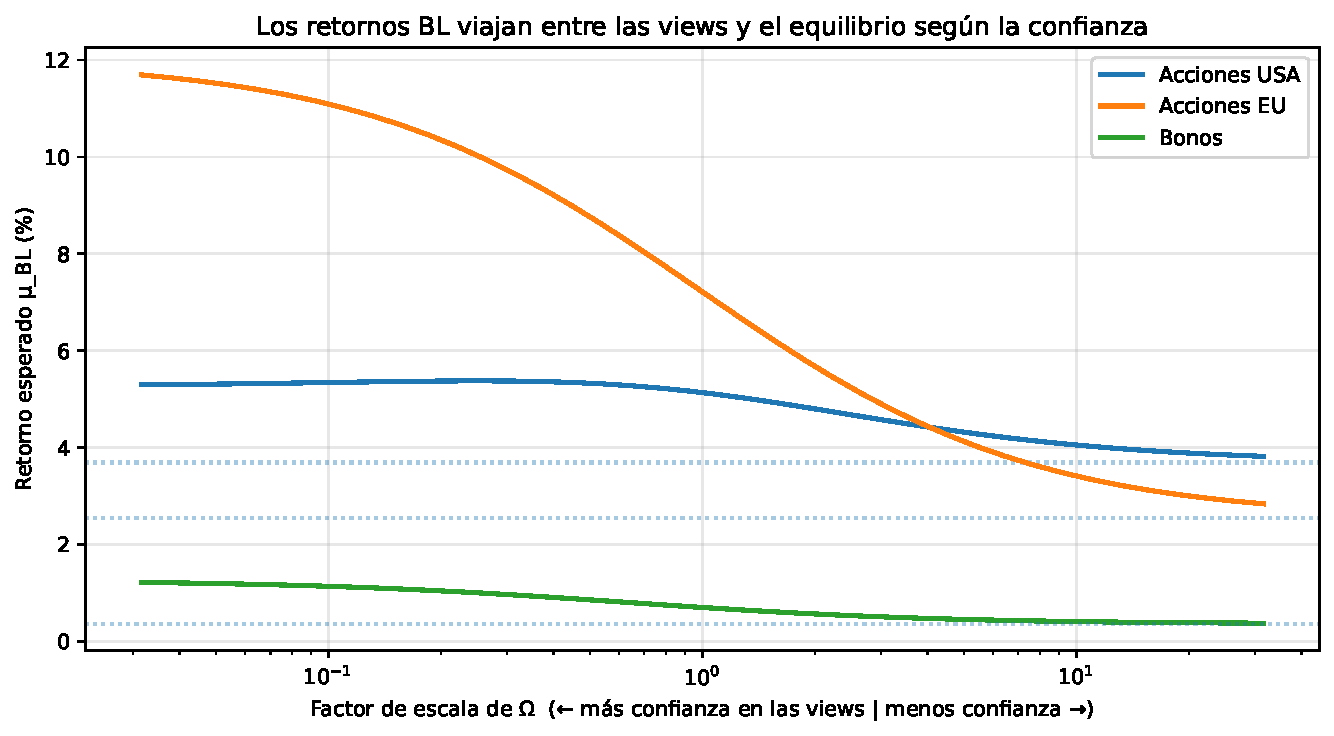
\includegraphics[keepaspectratio]{unidad2/cap10_black_litterman_files/figure-pdf/efecto-confianza-output-1.pdf}}

A la izquierda (mucha confianza) los retornos se acercan a lo que
afirman las views; a la derecha (poca confianza) vuelven a las líneas
punteadas del equilibrio. \textbf{El modelo nunca te deja ``irte'' más
allá de tus propias views ni ignorar del todo al mercado}: interpola
entre ambos de manera controlada.

\begin{center}\rule{0.5\linewidth}{0.5pt}\end{center}

\chapter{Recapitulando el flujo}\label{recapitulando-el-flujo}

El modelo completo es una tubería de cuatro pasos:

\begin{enumerate}
\def\labelenumi{\arabic{enumi}.}
\tightlist
\item
  \textbf{Equilibrio} →
  \(\boldsymbol{\Pi} = \delta \Sigma \mathbf{w}_{mkt}\) (la creencia de
  partida, gratis, desde el mercado).
\item
  \textbf{Views} → armar \(P\), \(Q\), \(\Omega\) (nuestras opiniones y
  su confianza).
\item
  \textbf{Fórmula maestra} → \(\boldsymbol{\mu}_{BL}\) (la mezcla
  ponderada por precisión).
\item
  \textbf{Optimización} → \(\mathbf{w}_{BL}\) (la cartera final).
\end{enumerate}

La gran ventaja: cada paso tiene una interpretación económica clara, y
en ningún momento tuvimos que inventar retornos esperados de la nada.
Por eso Black-Litterman es, todavía hoy, uno de los modelos de
asignación de activos más usados en la industria.

\begin{center}\rule{0.5\linewidth}{0.5pt}\end{center}

\chapter{Errores comunes}\label{errores-comunes-8}

\begin{tcolorbox}[enhanced jigsaw, bottomrule=.15mm, colback=white, opacitybacktitle=0.6, arc=.35mm, toprule=.15mm, opacityback=0, breakable, titlerule=0mm, left=2mm, coltitle=black, colbacktitle=quarto-callout-warning-color!10!white, colframe=quarto-callout-warning-color-frame, leftrule=.75mm, toptitle=1mm, bottomtitle=1mm, title=\textcolor{quarto-callout-warning-color}{\faExclamationTriangle}\hspace{0.5em}{Trampas frecuentes}, rightrule=.15mm]

\begin{itemize}
\tightlist
\item
  \textbf{Confundir \(\tau\) con \(\Omega\)}: \(\tau\) escala la
  incertidumbre \emph{global} del equilibrio; \(\Omega\) es la
  incertidumbre \emph{de cada view}. Son perillas distintas.
\item
  \textbf{Views inconsistentes con \(\Sigma\)}: si afirmás que dos
  activos altamente correlacionados se moverán en direcciones opuestas,
  el modelo hará contorsiones raras. Las views deberían ser coherentes
  con la estructura de covarianzas.
\item
  \textbf{Olvidar re-normalizar los pesos} o permitir cortos sin querer:
  siempre revisá que \(\mathbf{w}_{BL}\) sume 1 y respete tus
  restricciones.
\item
  \textbf{Invertir matrices con \texttt{inv} para resolver sistemas}:
  usá \texttt{np.linalg.solve}, que es más estable numéricamente que
  calcular la inversa y multiplicar.
\end{itemize}

\end{tcolorbox}

\begin{center}\rule{0.5\linewidth}{0.5pt}\end{center}

\chapter{Ejercicios Propuestos}\label{ejercicios-propuestos-9}

\begin{tcolorbox}[enhanced jigsaw, bottomrule=.15mm, colback=white, opacitybacktitle=0.6, arc=.35mm, toprule=.15mm, opacityback=0, breakable, titlerule=0mm, left=2mm, coltitle=black, colbacktitle=quarto-callout-important-color!10!white, colframe=quarto-callout-important-color-frame, leftrule=.75mm, toptitle=1mm, bottomtitle=1mm, title=\textcolor{quarto-callout-important-color}{\faExclamation}\hspace{0.5em}{Ejercicios}, rightrule=.15mm]

\begin{enumerate}
\def\labelenumi{\arabic{enumi}.}
\tightlist
\item
  \textbf{Sin views}: corré el modelo sin ninguna view (saltando la
  fórmula maestra, \(\boldsymbol{\mu}_{BL} = \boldsymbol{\Pi}\)) y
  verificá que \(\mathbf{w}_{BL}\) reproduce la cartera de mercado
  \(\mathbf{w}_{mkt}\).
\item
  \textbf{Subiendo la confianza}: reducí a la mitad los valores de
  \(\Omega\) y observá cómo \(\boldsymbol{\mu}_{BL}\) se acerca a \(Q\).
\item
  \textbf{View relativa pura}: eliminá la view absoluta y dejá solo
  ``USA supera a Bonos por 4\%''. ¿Cómo cambian los pesos frente al
  mercado? ¿Qué pasa con EU, sobre el que ya no opinás?
\item
  \textbf{Con restricciones}: usando \texttt{scipy.optimize.minimize},
  resolvé la cartera óptima con \(\boldsymbol{\mu}_{BL}\) imponiendo
  pesos no negativos que sumen 1, y compará con la solución cerrada.
\item
  \textbf{Cuarto activo}: extendé el universo a cuatro activos, definí
  una view sobre el nuevo y recalculá todo el pipeline.
\end{enumerate}

\end{tcolorbox}

Podés resolver estos ejercicios acá mismo: la celda ejecuta Python
\textbf{en tu navegador}, sin instalar nada (la primera ejecución tarda
unos segundos mientras carga el entorno; los paquetes que importes se
instalan solos).

\begin{Shaded}
\begin{Highlighting}[]
\NormalTok{\#| label: practica{-}navegador}
\NormalTok{import numpy as np}

\NormalTok{\# Tu solución acá...}
\end{Highlighting}
\end{Shaded}

\begin{center}\rule{0.5\linewidth}{0.5pt}\end{center}

\chapter{Referencias}\label{referencias-9}

\phantomsection\label{refs}

\part{Módulo 3: Riesgo, Simulación y Econometría}

\chapter*{Módulo 3: Riesgo, Simulación y
Econometría}\label{muxf3dulo-3-riesgo-simulaciuxf3n-y-econometruxeda-1}
\addcontentsline{toc}{chapter}{Módulo 3: Riesgo, Simulación y
Econometría}

\markboth{Módulo 3: Riesgo, Simulación y Econometría}{Módulo 3: Riesgo,
Simulación y Econometría}

\emph{Medir lo que puede salir mal y validar lo que creemos saber}

El Módulo 2 terminó con una advertencia: los modelos de portafolio son
tan buenos como sus supuestos, y los supuestos fallan. Este módulo ---el
más largo y diverso del libro--- se toma esa advertencia en serio y
construye el oficio completo del análisis cuantitativo de riesgo:
\textbf{medir la incertidumbre, simularla, modelarla y, sobre todo,
desconfiar de los propios modelos con método}.

El recorrido avanza en cuatro actos. Primero, la \textbf{medición del
riesgo} y su contexto institucional: el VaR y el Expected Shortfall como
lenguaje estándar (Capítulo 11), y el marco regulatorio que las crisis
fueron dejando ---Basilea III, stress testing--- junto a las dos
historias que todo analista debería saber contar: LTCM y 2008 (Capítulo
12). Segundo, los \textbf{modelos del mundo}: la simulación de Monte
Carlo con el Browniano geométrico (Capítulo 13) y su corrección
necesaria, los procesos con saltos y colas gruesas que describen los
mercados reales (Capítulo 14).

El tercer acto es la \textbf{inferencia}: cómo aprender de los datos con
modelos lineales bien especificados ---CAPM, multifactor, p-values
leídos con honestidad--- (Capítulo 15) y cómo modelar series que
dependen de su propio pasado con ARIMA y VAR (Capítulo 16). Y el cierre
es el acto que le da sentido a todo lo anterior: el \textbf{backtesting}
(Capítulo 17), la disciplina de separar la señal de la casualidad, que
convierte ``mi estrategia funcionó en el pasado'' en una afirmación
estadísticamente defendible\ldots{} o la desarma.

\begin{tcolorbox}[enhanced jigsaw, bottomrule=.15mm, colback=white, breakable, left=2mm, colframe=quarto-callout-note-color-frame, leftrule=.75mm, arc=.35mm, toprule=.15mm, rightrule=.15mm, opacityback=0]
\begin{minipage}[t]{5.5mm}
\textcolor{quarto-callout-note-color}{\faInfo}
\end{minipage}%
\begin{minipage}[t]{\textwidth - 5.5mm}

\vspace{-3mm}\textbf{El hilo conductor}\vspace{3mm}

Si tuviéramos que resumir el módulo en una frase, sería esta: \textbf{la
media y la varianza no cuentan la historia de las colas, y en las colas
vive el riesgo}. Cada capítulo ataca una consecuencia distinta de esa
frase.

\end{minipage}%
\end{tcolorbox}

\begin{center}\rule{0.5\linewidth}{0.5pt}\end{center}

\section*{🎯 Objetivos de Aprendizaje}\label{objetivos-de-aprendizaje-2}
\addcontentsline{toc}{section}{🎯 Objetivos de Aprendizaje}

\markright{🎯 Objetivos de Aprendizaje}

Al completar este módulo, vas a ser capaz de:

\begin{enumerate}
\def\labelenumi{\arabic{enumi}.}
\tightlist
\item
  \textbf{Calcular Value at Risk y Expected Shortfall} con métodos
  paramétrico, histórico y por Monte Carlo.
\item
  \textbf{Ubicar el riesgo en su marco regulatorio} (stress testing,
  Basilea III) y aprender de las crisis.
\item
  \textbf{Simular trayectorias de precios} con Browniano geométrico y
  modelos con saltos.
\item
  \textbf{Construir e interpretar modelos lineales} aplicados a finanzas
  (CAPM, multifactor).
\item
  \textbf{Modelar y pronosticar series de tiempo} con ARIMA y VAR.
\item
  \textbf{Validar estrategias} con backtesting out-of-sample y
  walk-forward.
\end{enumerate}

\begin{center}\rule{0.5\linewidth}{0.5pt}\end{center}

\section*{🗓️ Recorrido Capítulo a
Capítulo}\label{recorrido-capuxedtulo-a-capuxedtulo-2}
\addcontentsline{toc}{section}{🗓️ Recorrido Capítulo a Capítulo}

\markright{🗓️ Recorrido Capítulo a Capítulo}

\begin{longtable}[]{@{}
  >{\centering\arraybackslash}p{(\linewidth - 6\tabcolsep) * \real{0.2500}}
  >{\raggedright\arraybackslash}p{(\linewidth - 6\tabcolsep) * \real{0.1875}}
  >{\raggedright\arraybackslash}p{(\linewidth - 6\tabcolsep) * \real{0.2500}}
  >{\raggedright\arraybackslash}p{(\linewidth - 6\tabcolsep) * \real{0.3125}}@{}}
\toprule\noalign{}
\begin{minipage}[b]{\linewidth}\centering
Capítulo
\end{minipage} & \begin{minipage}[b]{\linewidth}\raggedright
Tema
\end{minipage} & \begin{minipage}[b]{\linewidth}\raggedright
Python
\end{minipage} & \begin{minipage}[b]{\linewidth}\raggedright
Finanzas
\end{minipage} \\
\midrule\noalign{}
\endhead
\bottomrule\noalign{}
\endlastfoot
\textbf{11} & VaR y Expected Shortfall & \texttt{scipy.stats},
\texttt{np.percentile} & VaR, CVaR/ES, backtesting de riesgo \\
\textbf{12} & Riesgo y Regulación & Simulación de escenarios & Stress
testing, Basilea III, LTCM, 2008 \\
\textbf{13} & Monte Carlo & Simulación vectorizada, \texttt{np.random} &
GBM, pricing por MC, convergencia \\
\textbf{14} & Procesos Estocásticos & Poisson, saltos & Jump-diffusion,
Lévy, colas gruesas \\
\textbf{15} & Econometría y Modelos Lineales & MCO, \texttt{statsmodels}
& CAPM, multifactor, p-values \\
\textbf{16} & Series Temporales & \texttt{statsmodels.tsa} & ARIMA, VAR,
estacionariedad \\
\textbf{17} & Backtesting & Ventanas rodantes & In/out-of-sample,
walk-forward, Sharpe OOS \\
\end{longtable}

\begin{center}\rule{0.5\linewidth}{0.5pt}\end{center}

\section*{🧰 Herramientas y
Librerías}\label{herramientas-y-libreruxedas-2}
\addcontentsline{toc}{section}{🧰 Herramientas y Librerías}

\markright{🧰 Herramientas y Librerías}

\textbf{NumPy}

Simulación vectorizada

\textbf{SciPy}

Distribuciones y tests

\textbf{Statsmodels}

Regresión y series de tiempo

\textbf{Matplotlib}

Distribuciones y trayectorias

\begin{center}\rule{0.5\linewidth}{0.5pt}\end{center}

\section*{🔑 Concepto Clave: VaR y Expected
Shortfall}\label{concepto-clave-var-y-expected-shortfall}
\addcontentsline{toc}{section}{🔑 Concepto Clave: VaR y Expected
Shortfall}

\markright{🔑 Concepto Clave: VaR y Expected Shortfall}

\begin{tcolorbox}[enhanced jigsaw, bottomrule=.15mm, colback=white, breakable, left=2mm, colframe=quarto-callout-important-color-frame, leftrule=.75mm, arc=.35mm, toprule=.15mm, rightrule=.15mm, opacityback=0]
\begin{minipage}[t]{5.5mm}
\textcolor{quarto-callout-important-color}{\faExclamation}
\end{minipage}%
\begin{minipage}[t]{\textwidth - 5.5mm}

El \textbf{Value at Risk} al nivel de confianza \(\alpha\) responde:
\emph{¿cuál es la pérdida que solo se excede el \((1-\alpha)\%\) de las
veces?}

\[VaR_\alpha = -(\mu + z_\alpha \cdot \sigma) \cdot W\]

Pero el VaR solo marca \textbf{dónde empieza} la zona de desastre. El
\textbf{Expected Shortfall} mira adentro: \emph{¿cuánto pierdo en
promedio cuando la cruzo?}

\[ES_\alpha = -E\big[\,r \mid r < -VaR_\alpha\,\big]\]

La tensión entre estas dos preguntas ---y por qué la regulación migró de
una a la otra--- es el punto de partida del módulo.

\end{minipage}%
\end{tcolorbox}

\begin{center}\rule{0.5\linewidth}{0.5pt}\end{center}

\section*{📚 Lecturas Recomendadas}\label{lecturas-recomendadas-2}
\addcontentsline{toc}{section}{📚 Lecturas Recomendadas}

\markright{📚 Lecturas Recomendadas}

\begin{itemize}
\tightlist
\item
  Jorion, P. (2006). \emph{Value at Risk}. McGraw-Hill.
\item
  Glasserman, P. (2003). \emph{Monte Carlo Methods in Financial
  Engineering}. Springer.
\item
  Wooldridge, J. (2019). \emph{Introductory Econometrics: A Modern
  Approach}. Cengage.
\item
  López de Prado, M. (2018). \emph{Advances in Financial Machine
  Learning}. Wiley.
\item
  Lowenstein, R. (2000). \emph{When Genius Failed}. Random House.
\end{itemize}

\chapter{Capítulo 11: Valor en Riesgo (VaR) y Expected
Shortfall}\label{capuxedtulo-11-valor-en-riesgo-var-y-expected-shortfall}

Medición de Riesgo de Mercado: VaR Paramétrico, Histórico y CVaR

Introducimos las herramientas fundamentales de medición de riesgo: VaR
paramétrico e histórico, Expected Shortfall (CVaR), volatilidad EWMA, y
tests de normalidad para entender las limitaciones de los modelos
gaussianos.

\hfill\break

\chapter{Introducción}\label{introducciuxf3n-8}

El \textbf{Value at Risk (VaR)} responde a la pregunta más importante en
gestión de riesgo:

\begin{quote}
\emph{¿Cuál es la máxima pérdida esperada en un horizonte dado, con un
nivel de confianza determinado?}
\end{quote}

\begin{tcolorbox}[enhanced jigsaw, bottomrule=.15mm, colback=white, opacitybacktitle=0.6, arc=.35mm, toprule=.15mm, opacityback=0, breakable, titlerule=0mm, left=2mm, coltitle=black, colbacktitle=quarto-callout-note-color!10!white, colframe=quarto-callout-note-color-frame, leftrule=.75mm, toptitle=1mm, bottomtitle=1mm, title=\textcolor{quarto-callout-note-color}{\faInfo}\hspace{0.5em}{Ejemplo intuitivo}, rightrule=.15mm]

Si el VaR diario al 95\% de un portafolio es \$150,000, significa que
\textbf{en 19 de cada 20 días}, la pérdida no superará esa cifra. Pero
en 1 de cada 20 días, sí podría.

\end{tcolorbox}

\begin{center}\rule{0.5\linewidth}{0.5pt}\end{center}

\chapter{Generación de Datos}\label{generaciuxf3n-de-datos}

Antes de calcular el VaR, necesitamos retornos. Simulamos un año de
retornos diarios:

\phantomsection\label{datos}
\begin{Shaded}
\begin{Highlighting}[]
\ImportTok{import}\NormalTok{ numpy }\ImportTok{as}\NormalTok{ np}
\ImportTok{import}\NormalTok{ matplotlib.pyplot }\ImportTok{as}\NormalTok{ plt}
\ImportTok{from}\NormalTok{ scipy }\ImportTok{import}\NormalTok{ stats}

\CommentTok{\# Configuración}
\NormalTok{rng }\OperatorTok{=}\NormalTok{ np.random.default\_rng(}\DecValTok{42}\NormalTok{)}
\NormalTok{valor\_portafolio }\OperatorTok{=} \DecValTok{10\_000\_000}  \CommentTok{\# $10M}

\CommentTok{\# Simular retornos diarios (252 días hábiles)}
\NormalTok{retornos }\OperatorTok{=}\NormalTok{ rng.normal(}\FloatTok{0.0004}\NormalTok{, }\FloatTok{0.015}\NormalTok{, }\DecValTok{252}\NormalTok{)}

\NormalTok{mu }\OperatorTok{=}\NormalTok{ np.mean(retornos)}
\NormalTok{sigma }\OperatorTok{=}\NormalTok{ np.std(retornos)}

\BuiltInTok{print}\NormalTok{(}\SpecialStringTok{f"Retornos diarios simulados: }\SpecialCharTok{\{}\BuiltInTok{len}\NormalTok{(retornos)}\SpecialCharTok{\}}\SpecialStringTok{ observaciones"}\NormalTok{)}
\BuiltInTok{print}\NormalTok{(}\SpecialStringTok{f"Media diaria: }\SpecialCharTok{\{}\NormalTok{mu}\SpecialCharTok{:.6f\}}\SpecialStringTok{ (}\SpecialCharTok{\{}\NormalTok{mu }\OperatorTok{*} \DecValTok{252}\SpecialCharTok{:.2\%\}}\SpecialStringTok{ anualizada)"}\NormalTok{)}
\BuiltInTok{print}\NormalTok{(}\SpecialStringTok{f"Volatilidad diaria: }\SpecialCharTok{\{}\NormalTok{sigma}\SpecialCharTok{:.6f\}}\SpecialStringTok{ (}\SpecialCharTok{\{}\NormalTok{sigma }\OperatorTok{*}\NormalTok{ np}\SpecialCharTok{.}\NormalTok{sqrt(}\DecValTok{252}\NormalTok{)}\SpecialCharTok{:.2\%\}}\SpecialStringTok{ anualizada)"}\NormalTok{)}
\end{Highlighting}
\end{Shaded}

\begin{verbatim}
Retornos diarios simulados: 252 observaciones
Media diaria: -0.000326 (-8.20% anualizada)
Volatilidad diaria: 0.014036 (22.28% anualizada)
\end{verbatim}

\begin{center}\rule{0.5\linewidth}{0.5pt}\end{center}

\chapter{VaR Paramétrico (Normal)}\label{var-paramuxe9trico-normal}

El primer método es el más rápido y el que más supuestos hace: asumir
que los retornos siguen una \textbf{distribución normal}. Si eso es
cierto, la distribución entera queda descripta por dos números que ya
estimamos ---media \(\mu\) y desvío \(\sigma\)--- y el cuantil que
define el VaR tiene fórmula cerrada:

\[VaR_{\alpha} = -(\mu + z_\alpha \cdot \sigma) \cdot W\]

donde \(z_\alpha\) es el cuantil de la normal estándar (para 95\%,
\(z = -1.645\): el punto que deja el 5\% de la campana a su izquierda) y
\(W\) es el valor del portafolio.

\phantomsection\label{var-parametrico}
\begin{Shaded}
\begin{Highlighting}[]
\NormalTok{confianza }\OperatorTok{=} \FloatTok{0.95}

\CommentTok{\# Z{-}score para 95\%}
\NormalTok{z }\OperatorTok{=}\NormalTok{ stats.norm.ppf(}\DecValTok{1} \OperatorTok{{-}}\NormalTok{ confianza)}

\CommentTok{\# VaR paramétrico (1 día)}
\NormalTok{var\_param\_95 }\OperatorTok{=} \OperatorTok{{-}}\NormalTok{(mu }\OperatorTok{+}\NormalTok{ z }\OperatorTok{*}\NormalTok{ sigma) }\OperatorTok{*}\NormalTok{ valor\_portafolio}

\CommentTok{\# También al 99\%}
\NormalTok{z\_99 }\OperatorTok{=}\NormalTok{ stats.norm.ppf(}\FloatTok{0.01}\NormalTok{)}
\NormalTok{var\_param\_99 }\OperatorTok{=} \OperatorTok{{-}}\NormalTok{(mu }\OperatorTok{+}\NormalTok{ z\_99 }\OperatorTok{*}\NormalTok{ sigma) }\OperatorTok{*}\NormalTok{ valor\_portafolio}

\BuiltInTok{print}\NormalTok{(}\SpecialStringTok{f"VaR Paramétrico (95\%, 1 día): $}\SpecialCharTok{\{}\NormalTok{var\_param\_95}\SpecialCharTok{:\textgreater{}12,.2f\}}\SpecialStringTok{"}\NormalTok{)}
\BuiltInTok{print}\NormalTok{(}\SpecialStringTok{f"VaR Paramétrico (99\%, 1 día): $}\SpecialCharTok{\{}\NormalTok{var\_param\_99}\SpecialCharTok{:\textgreater{}12,.2f\}}\SpecialStringTok{"}\NormalTok{)}
\BuiltInTok{print}\NormalTok{(}\SpecialStringTok{f"Como \% del portafolio (95\%):  }\SpecialCharTok{\{}\NormalTok{var\_param\_95 }\OperatorTok{/}\NormalTok{ valor\_portafolio}\SpecialCharTok{:.4\%\}}\SpecialStringTok{"}\NormalTok{)}
\BuiltInTok{print}\NormalTok{(}\SpecialStringTok{f"Como \% del portafolio (99\%):  }\SpecialCharTok{\{}\NormalTok{var\_param\_99 }\OperatorTok{/}\NormalTok{ valor\_portafolio}\SpecialCharTok{:.4\%\}}\SpecialStringTok{"}\NormalTok{)}
\end{Highlighting}
\end{Shaded}

\begin{verbatim}
VaR Paramétrico (95%, 1 día): $  234,134.38
VaR Paramétrico (99%, 1 día): $  329,791.90
Como % del portafolio (95%):  2.3413%
Como % del portafolio (99%):  3.2979%
\end{verbatim}

Traduzcamos el número a castellano, porque es lo que te van a pedir en
cualquier comité de riesgo: \emph{``con un portafolio de \$10 millones,
en 19 de cada 20 días la pérdida no debería superar los
\textasciitilde\$240.000 (un 2.4\% del portafolio)''}. Y la comparación
entre niveles enseña algo general: pasar del 95\% al 99\% de confianza
\textbf{encarece el VaR en casi un 50\%} --- meterse más adentro de la
cola cuesta cada vez más caro, porque la cola se estira.

\begin{center}\rule{0.5\linewidth}{0.5pt}\end{center}

\chapter{VaR Histórico}\label{var-histuxf3rico}

El método paramétrico se apoya por completo en el supuesto de
normalidad. El \textbf{VaR histórico} toma el camino opuesto: no asume
\emph{ninguna} distribución --- deja que los datos hablen solos. La
receta es de una simplicidad brutal: ordenás los retornos observados de
peor a mejor y leés el percentil correspondiente. El VaR 95\% es,
literalmente, ``el retorno del día que está en el puesto 5\% de los
peores''.

\phantomsection\label{var-historico}
\begin{Shaded}
\begin{Highlighting}[]
\CommentTok{\# VaR Histórico: percentil de los retornos reales}
\NormalTok{percentil\_5 }\OperatorTok{=}\NormalTok{ np.percentile(retornos, }\DecValTok{5}\NormalTok{)}
\NormalTok{percentil\_1 }\OperatorTok{=}\NormalTok{ np.percentile(retornos, }\DecValTok{1}\NormalTok{)}

\NormalTok{var\_hist\_95 }\OperatorTok{=} \OperatorTok{{-}}\NormalTok{percentil\_5 }\OperatorTok{*}\NormalTok{ valor\_portafolio}
\NormalTok{var\_hist\_99 }\OperatorTok{=} \OperatorTok{{-}}\NormalTok{percentil\_1 }\OperatorTok{*}\NormalTok{ valor\_portafolio}

\BuiltInTok{print}\NormalTok{(}\SpecialStringTok{f"VaR Histórico (95\%, 1 día): $}\SpecialCharTok{\{}\NormalTok{var\_hist\_95}\SpecialCharTok{:\textgreater{}12,.2f\}}\SpecialStringTok{"}\NormalTok{)}
\BuiltInTok{print}\NormalTok{(}\SpecialStringTok{f"VaR Histórico (99\%, 1 día): $}\SpecialCharTok{\{}\NormalTok{var\_hist\_99}\SpecialCharTok{:\textgreater{}12,.2f\}}\SpecialStringTok{"}\NormalTok{)}
\end{Highlighting}
\end{Shaded}

\begin{verbatim}
VaR Histórico (95%, 1 día): $  213,744.80
VaR Histórico (99%, 1 día): $  295,941.84
\end{verbatim}

Con nuestros datos, el histórico da parecido al paramétrico --- lógico,
porque los retornos \emph{fueron simulados} de una normal. Con retornos
reales (colas pesadas), el histórico al 99\% suele salir \textbf{más
alto}, porque los peores días de la muestra son peores de lo que la
normal admite. Esa diferencia entre métodos no es un defecto: es un
\textbf{diagnóstico} --- cuando el histórico y el paramétrico divergen,
la distribución real se está apartando de la normal justo donde más
importa.

El precio de la flexibilidad del histórico: al 99\% con un año de datos
(252 observaciones), el percentil 1 se estima con \textbf{apenas 2 o 3
observaciones}. Tu medida de riesgo cuelga de un puñado de días --- por
eso en la práctica se usan ventanas más largas o métodos híbridos.

\begin{center}\rule{0.5\linewidth}{0.5pt}\end{center}

\chapter{Comparación Visual: Paramétrico
vs.~Histórico}\label{comparaciuxf3n-visual-paramuxe9trico-vs.-histuxf3rico}

\begin{Shaded}
\begin{Highlighting}[]
\NormalTok{fig, ax }\OperatorTok{=}\NormalTok{ plt.subplots(figsize}\OperatorTok{=}\NormalTok{(}\DecValTok{10}\NormalTok{, }\DecValTok{5}\NormalTok{))}

\CommentTok{\# Histograma de retornos}
\NormalTok{ax.hist(retornos, bins}\OperatorTok{=}\DecValTok{40}\NormalTok{, density}\OperatorTok{=}\VariableTok{True}\NormalTok{, alpha}\OperatorTok{=}\FloatTok{0.6}\NormalTok{, color}\OperatorTok{=}\StringTok{"\#2d6a9f"}\NormalTok{, }
\NormalTok{        edgecolor}\OperatorTok{=}\StringTok{"white"}\NormalTok{, label}\OperatorTok{=}\StringTok{"Retornos observados"}\NormalTok{)}

\CommentTok{\# Curva normal teórica}
\NormalTok{x }\OperatorTok{=}\NormalTok{ np.linspace(retornos.}\BuiltInTok{min}\NormalTok{(), retornos.}\BuiltInTok{max}\NormalTok{(), }\DecValTok{200}\NormalTok{)}
\NormalTok{ax.plot(x, stats.norm.pdf(x, mu, sigma), color}\OperatorTok{=}\StringTok{"\#1e3a5f"}\NormalTok{, linewidth}\OperatorTok{=}\DecValTok{2}\NormalTok{, }
\NormalTok{        label}\OperatorTok{=}\StringTok{"Normal teórica"}\NormalTok{)}

\CommentTok{\# Líneas de VaR}
\NormalTok{ax.axvline(percentil\_5, color}\OperatorTok{=}\StringTok{"\#ef4444"}\NormalTok{, linewidth}\OperatorTok{=}\DecValTok{2}\NormalTok{, linestyle}\OperatorTok{=}\StringTok{"{-}{-}"}\NormalTok{, }
\NormalTok{           label}\OperatorTok{=}\SpecialStringTok{f"VaR Hist 95\% (}\SpecialCharTok{\{}\NormalTok{percentil\_5}\SpecialCharTok{:.4f\}}\SpecialStringTok{)"}\NormalTok{)}
\NormalTok{ax.axvline(mu }\OperatorTok{+}\NormalTok{ z }\OperatorTok{*}\NormalTok{ sigma, color}\OperatorTok{=}\StringTok{"\#f59e0b"}\NormalTok{, linewidth}\OperatorTok{=}\DecValTok{2}\NormalTok{, linestyle}\OperatorTok{=}\StringTok{":"}\NormalTok{, }
\NormalTok{           label}\OperatorTok{=}\SpecialStringTok{f"VaR Param 95\% (}\SpecialCharTok{\{}\NormalTok{mu }\OperatorTok{+}\NormalTok{ z }\OperatorTok{*}\NormalTok{ sigma}\SpecialCharTok{:.4f\}}\SpecialStringTok{)"}\NormalTok{)}

\NormalTok{ax.set\_xlabel(}\StringTok{"Retorno Diario"}\NormalTok{)}
\NormalTok{ax.set\_ylabel(}\StringTok{"Densidad"}\NormalTok{)}
\NormalTok{ax.set\_title(}\StringTok{"Distribución de Retornos con Líneas de VaR"}\NormalTok{)}
\NormalTok{ax.legend(fontsize}\OperatorTok{=}\DecValTok{9}\NormalTok{)}
\NormalTok{ax.grid(}\VariableTok{True}\NormalTok{, alpha}\OperatorTok{=}\FloatTok{0.3}\NormalTok{)}
\NormalTok{plt.tight\_layout()}
\NormalTok{plt.show()}
\end{Highlighting}
\end{Shaded}

\pandocbounded{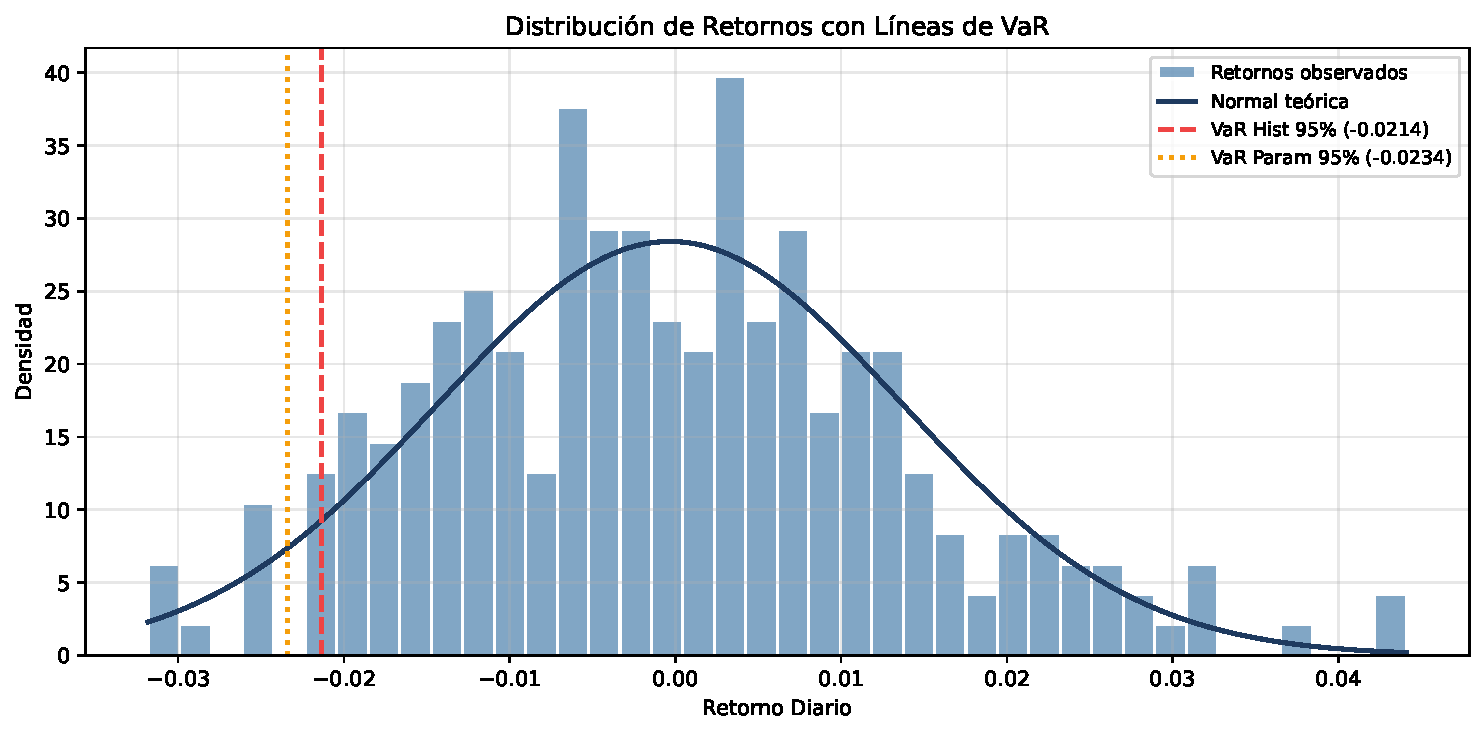
\includegraphics[keepaspectratio]{unidad3/cap11_var_expected_shortfall_files/figure-pdf/comparacion-var-output-1.pdf}}

\begin{tcolorbox}[enhanced jigsaw, bottomrule=.15mm, colback=white, opacitybacktitle=0.6, arc=.35mm, toprule=.15mm, opacityback=0, breakable, titlerule=0mm, left=2mm, coltitle=black, colbacktitle=quarto-callout-warning-color!10!white, colframe=quarto-callout-warning-color-frame, leftrule=.75mm, toptitle=1mm, bottomtitle=1mm, title=\textcolor{quarto-callout-warning-color}{\faExclamationTriangle}\hspace{0.5em}{Diferencias entre métodos}, rightrule=.15mm]

El VaR paramétrico y el histórico \textbf{no necesariamente coinciden}.
La diferencia se agranda cuando la distribución real se desvía de la
normal (colas pesadas, asimetría).

\end{tcolorbox}

\begin{center}\rule{0.5\linewidth}{0.5pt}\end{center}

\chapter{Expected Shortfall (CVaR): mirar dentro de la
cola}\label{expected-shortfall-cvar-mirar-dentro-de-la-cola}

El VaR tiene un defecto conceptual serio: te dice \emph{dónde empieza}
la zona de desastre, pero \textbf{no te dice nada de lo que pasa
adentro}. Dos portafolios pueden tener el mismo VaR al 95\% y
comportamientos totalmente distintos en ese 5\% restante: uno pierde
apenas un poco más que el VaR, el otro se pulveriza. Para el VaR, son
idénticos.

El \textbf{Expected Shortfall} (ES), también llamado \textbf{CVaR}
(\emph{Conditional Value at Risk}), corrige exactamente eso. Su pregunta
es:

\begin{quote}
\emph{En los peores escenarios ---los que superan el VaR---, ¿cuánto
pierdo \textbf{en promedio}?}
\end{quote}

\[ES_\alpha = -E\big[\,r \mid r < -VaR_\alpha\,\big]\]

Es una esperanza \textbf{condicional}: promediamos los retornos
\emph{dado que} caímos en la cola. Por construcción, el ES siempre es
mayor o igual que el VaR --- es el ``qué tan feo se pone'' después de
cruzar la frontera.

\section{Cálculo histórico: promediar la
cola}\label{cuxe1lculo-histuxf3rico-promediar-la-cola}

Con el método histórico, el cálculo es de una transparencia total:
filtrás los días peores que el VaR y promediás.

\phantomsection\label{cvar}
\begin{Shaded}
\begin{Highlighting}[]
\CommentTok{\# ES histórico: media de los retornos por debajo del percentil correspondiente}
\NormalTok{retornos\_cola }\OperatorTok{=}\NormalTok{ retornos[retornos }\OperatorTok{\textless{}}\NormalTok{ percentil\_5]}
\NormalTok{cvar\_95 }\OperatorTok{=} \OperatorTok{{-}}\NormalTok{np.mean(retornos\_cola) }\OperatorTok{*}\NormalTok{ valor\_portafolio}

\NormalTok{retornos\_cola\_99 }\OperatorTok{=}\NormalTok{ retornos[retornos }\OperatorTok{\textless{}}\NormalTok{ percentil\_1]}
\NormalTok{cvar\_99 }\OperatorTok{=} \OperatorTok{{-}}\NormalTok{np.mean(retornos\_cola\_99) }\OperatorTok{*}\NormalTok{ valor\_portafolio}

\BuiltInTok{print}\NormalTok{(}\SpecialStringTok{f"Días en la cola del 5\%: }\SpecialCharTok{\{}\BuiltInTok{len}\NormalTok{(retornos\_cola)}\SpecialCharTok{\}}\SpecialStringTok{"}\NormalTok{)}
\BuiltInTok{print}\NormalTok{(}\SpecialStringTok{f"ES/CVaR (95\%, 1 día): $}\SpecialCharTok{\{}\NormalTok{cvar\_95}\SpecialCharTok{:\textgreater{}12,.2f\}}\SpecialStringTok{   (VaR hist: $}\SpecialCharTok{\{}\NormalTok{var\_hist\_95}\SpecialCharTok{:,.2f\}}\SpecialStringTok{)"}\NormalTok{)}
\BuiltInTok{print}\NormalTok{(}\SpecialStringTok{f"ES/CVaR (99\%, 1 día): $}\SpecialCharTok{\{}\NormalTok{cvar\_99}\SpecialCharTok{:\textgreater{}12,.2f\}}\SpecialStringTok{   (VaR hist: $}\SpecialCharTok{\{}\NormalTok{var\_hist\_99}\SpecialCharTok{:,.2f\}}\SpecialStringTok{)"}\NormalTok{)}
\BuiltInTok{print}\NormalTok{(}\SpecialStringTok{f"}\CharTok{\textbackslash{}n}\SpecialStringTok{El ES 95\% es }\SpecialCharTok{\{}\NormalTok{cvar\_95}\OperatorTok{/}\NormalTok{var\_hist\_95}\SpecialCharTok{:.2f\}}\SpecialStringTok{x el VaR 95\%"}\NormalTok{)}
\BuiltInTok{print}\NormalTok{(}\StringTok{"→ Cuando el día es malo de verdad, la pérdida promedio supera al VaR en ese factor."}\NormalTok{)}
\end{Highlighting}
\end{Shaded}

\begin{verbatim}
Días en la cola del 5%: 13
ES/CVaR (95%, 1 día): $  257,564.55   (VaR hist: $213,744.80)
ES/CVaR (99%, 1 día): $  312,475.37   (VaR hist: $295,941.84)

El ES 95% es 1.21x el VaR 95%
→ Cuando el día es malo de verdad, la pérdida promedio supera al VaR en ese factor.
\end{verbatim}

\section{Cálculo paramétrico: fórmula cerrada bajo
normalidad}\label{cuxe1lculo-paramuxe9trico-fuxf3rmula-cerrada-bajo-normalidad}

Si asumimos retornos normales, el ES también tiene fórmula cerrada. Para
nivel de confianza \(\alpha\):

\[ES_\alpha = -\left(\mu - \sigma \cdot \frac{\phi(z_{1-\alpha})}{1-\alpha}\right) \cdot W\]

donde \(\phi\) es la densidad normal estándar y \(z_{1-\alpha}\) el
cuantil. El cociente \(\phi(z)/(1-\alpha)\) es la ``media de la cola''
de la normal.

\phantomsection\label{es-parametrico}
\begin{Shaded}
\begin{Highlighting}[]
\NormalTok{alpha }\OperatorTok{=} \FloatTok{0.95}
\NormalTok{z\_a }\OperatorTok{=}\NormalTok{ stats.norm.ppf(}\DecValTok{1} \OperatorTok{{-}}\NormalTok{ alpha)}

\NormalTok{es\_param\_95 }\OperatorTok{=} \OperatorTok{{-}}\NormalTok{(mu }\OperatorTok{{-}}\NormalTok{ sigma }\OperatorTok{*}\NormalTok{ stats.norm.pdf(z\_a) }\OperatorTok{/}\NormalTok{ (}\DecValTok{1} \OperatorTok{{-}}\NormalTok{ alpha)) }\OperatorTok{*}\NormalTok{ valor\_portafolio}
\BuiltInTok{print}\NormalTok{(}\SpecialStringTok{f"ES paramétrico (95\%): $}\SpecialCharTok{\{}\NormalTok{es\_param\_95}\SpecialCharTok{:\textgreater{}12,.2f\}}\SpecialStringTok{"}\NormalTok{)}
\BuiltInTok{print}\NormalTok{(}\SpecialStringTok{f"ES histórico   (95\%): $}\SpecialCharTok{\{}\NormalTok{cvar\_95}\SpecialCharTok{:\textgreater{}12,.2f\}}\SpecialStringTok{"}\NormalTok{)}
\end{Highlighting}
\end{Shaded}

\begin{verbatim}
ES paramétrico (95%): $  292,786.93
ES histórico   (95%): $  257,564.55
\end{verbatim}

Ambos métodos deberían parecerse con datos \textasciitilde normales como
los nuestros. Con retornos reales (colas pesadas), el histórico suele
dar \textbf{más alto} --- y es el que está diciendo la verdad. También
se puede estimar el ES por \textbf{Monte Carlo}: simulás miles de
retornos del modelo que quieras (con saltos, con t-Student) y promediás
la cola simulada; lo haremos en el Capítulo 13.

\section{Por qué el ES es ``coherente'' y el VaR
no}\label{por-quuxe9-el-es-es-coherente-y-el-var-no}

Hay un argumento matemático de fondo, y vale la pena entenderlo porque
explica por qué \textbf{Basilea cambió del VaR al ES} para riesgo de
mercado.

Una medida de riesgo razonable debería premiar la diversificación: el
riesgo de una cartera combinada no debería superar la suma de los
riesgos individuales. Esa propiedad se llama \textbf{subaditividad}:

\[\rho(A + B) \;\le\; \rho(A) + \rho(B)\]

El VaR \textbf{puede violarla}. El ejemplo clásico: dos bonos
independientes que rara vez caen en default, pero cuando caen, pierden
mucho.

\phantomsection\label{subaditividad}
\begin{Shaded}
\begin{Highlighting}[]
\CommentTok{\# Dos bonos independientes: 3\% de probabilidad de default con pérdida del 60\%}
\NormalTok{rng\_b }\OperatorTok{=}\NormalTok{ np.random.default\_rng(}\DecValTok{7}\NormalTok{)}
\NormalTok{n\_esc }\OperatorTok{=} \DecValTok{100\_000}

\KeywordTok{def}\NormalTok{ perdida\_bono(rng, n):}
\NormalTok{    default }\OperatorTok{=}\NormalTok{ rng.random(n) }\OperatorTok{\textless{}} \FloatTok{0.03}
    \ControlFlowTok{return}\NormalTok{ np.where(default, }\OperatorTok{{-}}\FloatTok{0.60}\NormalTok{, }\FloatTok{0.02}\NormalTok{)   }\CommentTok{\# {-}60\% si default, +2\% si no}

\NormalTok{r\_A }\OperatorTok{=}\NormalTok{ perdida\_bono(rng\_b, n\_esc)}
\NormalTok{r\_B }\OperatorTok{=}\NormalTok{ perdida\_bono(rng\_b, n\_esc)}
\NormalTok{r\_AB }\OperatorTok{=} \FloatTok{0.5} \OperatorTok{*}\NormalTok{ r\_A }\OperatorTok{+} \FloatTok{0.5} \OperatorTok{*}\NormalTok{ r\_B                }\CommentTok{\# cartera diversificada 50/50}

\KeywordTok{def}\NormalTok{ var\_h(r, conf}\OperatorTok{=}\FloatTok{0.95}\NormalTok{):}
    \ControlFlowTok{return} \OperatorTok{{-}}\NormalTok{np.percentile(r, (}\DecValTok{1} \OperatorTok{{-}}\NormalTok{ conf) }\OperatorTok{*} \DecValTok{100}\NormalTok{)}

\KeywordTok{def}\NormalTok{ es\_h(r, conf}\OperatorTok{=}\FloatTok{0.95}\NormalTok{):}
\NormalTok{    umbral }\OperatorTok{=}\NormalTok{ np.percentile(r, (}\DecValTok{1} \OperatorTok{{-}}\NormalTok{ conf) }\OperatorTok{*} \DecValTok{100}\NormalTok{)}
    \ControlFlowTok{return} \OperatorTok{{-}}\NormalTok{r[r }\OperatorTok{\textless{}=}\NormalTok{ umbral].mean()}

\BuiltInTok{print}\NormalTok{(}\SpecialStringTok{f"}\SpecialCharTok{\{}\StringTok{\textquotesingle{}\textquotesingle{}}\SpecialCharTok{:18\}\{}\StringTok{\textquotesingle{}Bono A\textquotesingle{}}\SpecialCharTok{:\textgreater{}9\}\{}\StringTok{\textquotesingle{}Bono B\textquotesingle{}}\SpecialCharTok{:\textgreater{}9\}\{}\StringTok{\textquotesingle{}Cartera 50/50\textquotesingle{}}\SpecialCharTok{:\textgreater{}15\}}\SpecialStringTok{"}\NormalTok{)}
\BuiltInTok{print}\NormalTok{(}\SpecialStringTok{f"}\SpecialCharTok{\{}\StringTok{\textquotesingle{}VaR 95\%\textquotesingle{}}\SpecialCharTok{:\textless{}18\}\{}\NormalTok{var\_h(r\_A)}\SpecialCharTok{:\textgreater{}9.1\%\}\{}\NormalTok{var\_h(r\_B)}\SpecialCharTok{:\textgreater{}9.1\%\}\{}\NormalTok{var\_h(r\_AB)}\SpecialCharTok{:\textgreater{}15.1\%\}}\SpecialStringTok{"}\NormalTok{)}
\BuiltInTok{print}\NormalTok{(}\SpecialStringTok{f"}\SpecialCharTok{\{}\StringTok{\textquotesingle{}ES  95\%\textquotesingle{}}\SpecialCharTok{:\textless{}18\}\{}\NormalTok{es\_h(r\_A)}\SpecialCharTok{:\textgreater{}9.1\%\}\{}\NormalTok{es\_h(r\_B)}\SpecialCharTok{:\textgreater{}9.1\%\}\{}\NormalTok{es\_h(r\_AB)}\SpecialCharTok{:\textgreater{}15.1\%\}}\SpecialStringTok{"}\NormalTok{)}
\end{Highlighting}
\end{Shaded}

\begin{verbatim}
                     Bono A   Bono B  Cartera 50/50
VaR 95%               -2.0%    -2.0%          29.0%
ES  95%               -0.2%    -0.2%          29.5%
\end{verbatim}

Mirá el resultado con atención, porque es contraintuitivo: cada bono
individual tiene \textbf{VaR negativo o nulo} (la probabilidad de
default, 3\%, es menor que el 5\% de la cola, así que el VaR ``no ve''
el default). Pero la cartera diversificada tiene VaR \textbf{positivo y
grande}: al combinar dos bonos, la probabilidad de que \emph{al menos
uno} caiga (\textasciitilde6\%) ya asoma dentro de la cola del 5\%.

Según el VaR, \textbf{diversificar empeoró el riesgo} --- un absurdo
económico. El ES, en cambio, ve el default de cada bono individual
(porque promedia toda la cola, no solo mira la frontera) y reporta
correctamente que la cartera combinada es menos riesgosa que cada bono
solo. Esa es la diferencia entre una medida coherente y una que no lo
es.

\begin{tcolorbox}[enhanced jigsaw, bottomrule=.15mm, colback=white, opacitybacktitle=0.6, arc=.35mm, toprule=.15mm, opacityback=0, breakable, titlerule=0mm, left=2mm, coltitle=black, colbacktitle=quarto-callout-important-color!10!white, colframe=quarto-callout-important-color-frame, leftrule=.75mm, toptitle=1mm, bottomtitle=1mm, title=\textcolor{quarto-callout-important-color}{\faExclamation}\hspace{0.5em}{VaR vs.~Expected Shortfall, en síntesis}, rightrule=.15mm]

\begin{longtable}[]{@{}
  >{\raggedright\arraybackslash}p{(\linewidth - 6\tabcolsep) * \real{0.2195}}
  >{\raggedright\arraybackslash}p{(\linewidth - 6\tabcolsep) * \real{0.5366}}
  >{\centering\arraybackslash}p{(\linewidth - 6\tabcolsep) * \real{0.1220}}
  >{\centering\arraybackslash}p{(\linewidth - 6\tabcolsep) * \real{0.1220}}@{}}
\toprule\noalign{}
\begin{minipage}[b]{\linewidth}\raggedright
Métrica
\end{minipage} & \begin{minipage}[b]{\linewidth}\raggedright
Pregunta que responde
\end{minipage} & \begin{minipage}[b]{\linewidth}\centering
¿Subaditiva?
\end{minipage} & \begin{minipage}[b]{\linewidth}\centering
¿Ve dentro de la cola?
\end{minipage} \\
\midrule\noalign{}
\endhead
\bottomrule\noalign{}
\endlastfoot
\textbf{VaR} & ¿Dónde empieza la zona de pérdidas extremas? & No siempre
& No \\
\textbf{ES/CVaR} & ¿Cuánto pierdo en promedio cuando estoy en esa zona?
& Sí (coherente) & Sí \\
\end{longtable}

Por estas propiedades, \textbf{Basilea III (FRTB)} reemplazó el VaR 99\%
por el \textbf{ES 97.5\%} como métrica regulatoria de riesgo de mercado.
En la práctica profesional se reportan ambos: el VaR por tradición y
comparabilidad, el ES por honestidad sobre las colas.

\end{tcolorbox}

\begin{center}\rule{0.5\linewidth}{0.5pt}\end{center}

\chapter{Backtesting de VaR: ¿el modelo dice la
verdad?}\label{backtesting-de-var-el-modelo-dice-la-verdad}

Calculamos un VaR 95\%. ¿Cómo sabemos si es \emph{correcto}? Hay una
forma directa de auditarlo, y es la que exigen los reguladores: contar.
Si el VaR 95\% está bien calibrado, la pérdida real debería superarlo
\textbf{el 5\% de los días} --- ni mucho más (el modelo subestima el
riesgo) ni mucho menos (lo sobreestima, y estás inmovilizando capital de
más). Cada día en que la pérdida supera al VaR se llama una
\textbf{excepción}.

El \textbf{test de Kupiec} (o \emph{proportion of failures}) formaliza
el conteo. Su lógica: si cada día hay una probabilidad del 5\% de
excepción, y los días son independientes, el número total de excepciones
en \(n\) días sigue una \textbf{distribución binomial} --- igual que
contar caras en tiradas de una moneda cargada al 5\%. Con eso podemos
preguntar: \emph{¿el número de excepciones que observé es compatible con
esa binomial?} Si observamos demasiadas, la probabilidad de que el
modelo esté bien calibrado (el p-value) se hace chica y lo rechazamos.

\phantomsection\label{backtesting}
\begin{Shaded}
\begin{Highlighting}[]
\CommentTok{\# Contar cuántos días la pérdida real superó al VaR}
\NormalTok{var\_limite }\OperatorTok{=}\NormalTok{ mu }\OperatorTok{+}\NormalTok{ z }\OperatorTok{*}\NormalTok{ sigma  }\CommentTok{\# VaR paramétrico expresado como retorno}
\NormalTok{excepciones }\OperatorTok{=}\NormalTok{ np.}\BuiltInTok{sum}\NormalTok{(retornos }\OperatorTok{\textless{}}\NormalTok{ var\_limite)}
\NormalTok{tasa\_excepciones }\OperatorTok{=}\NormalTok{ excepciones }\OperatorTok{/} \BuiltInTok{len}\NormalTok{(retornos)}

\BuiltInTok{print}\NormalTok{(}\SpecialStringTok{f"Excepciones: }\SpecialCharTok{\{}\NormalTok{excepciones}\SpecialCharTok{\}}\SpecialStringTok{ de }\SpecialCharTok{\{}\BuiltInTok{len}\NormalTok{(retornos)}\SpecialCharTok{\}}\SpecialStringTok{ días"}\NormalTok{)}
\BuiltInTok{print}\NormalTok{(}\SpecialStringTok{f"Tasa de excepciones: }\SpecialCharTok{\{}\NormalTok{tasa\_excepciones}\SpecialCharTok{:.2\%\}}\SpecialStringTok{"}\NormalTok{)}
\BuiltInTok{print}\NormalTok{(}\SpecialStringTok{f"Tasa esperada:       }\SpecialCharTok{\{}\DecValTok{1} \OperatorTok{{-}}\NormalTok{ confianza}\SpecialCharTok{:.2\%\}}\SpecialStringTok{"}\NormalTok{)}
\BuiltInTok{print}\NormalTok{(}\SpecialStringTok{f"Excepciones esperadas: }\SpecialCharTok{\{}\BuiltInTok{len}\NormalTok{(retornos) }\OperatorTok{*}\NormalTok{ (}\DecValTok{1} \OperatorTok{{-}}\NormalTok{ confianza)}\SpecialCharTok{:.1f\}}\SpecialStringTok{"}\NormalTok{)}

\CommentTok{\# Test de Kupiec: ¿el número de excepciones es compatible con una binomial(n, 5\%)?}
\ImportTok{from}\NormalTok{ scipy.stats }\ImportTok{import}\NormalTok{ binom}
\NormalTok{p\_value }\OperatorTok{=} \DecValTok{1} \OperatorTok{{-}}\NormalTok{ binom.cdf(excepciones }\OperatorTok{{-}} \DecValTok{1}\NormalTok{, }\BuiltInTok{len}\NormalTok{(retornos), }\DecValTok{1} \OperatorTok{{-}}\NormalTok{ confianza)}
\BuiltInTok{print}\NormalTok{(}\SpecialStringTok{f"}\CharTok{\textbackslash{}n}\SpecialStringTok{p{-}value (Kupiec): }\SpecialCharTok{\{}\NormalTok{p\_value}\SpecialCharTok{:.4f\}}\SpecialStringTok{"}\NormalTok{)}
\BuiltInTok{print}\NormalTok{(}\StringTok{"Aprobado"} \ControlFlowTok{if}\NormalTok{ p\_value }\OperatorTok{\textgreater{}} \FloatTok{0.05} \ControlFlowTok{else} \StringTok{"Rechazado: demasiadas excepciones"}\NormalTok{)}
\end{Highlighting}
\end{Shaded}

\begin{verbatim}
Excepciones: 9 de 252 días
Tasa de excepciones: 3.57%
Tasa esperada:       5.00%
Excepciones esperadas: 12.6

p-value (Kupiec): 0.8867
Aprobado
\end{verbatim}

Interpretemos el resultado: esperábamos \textasciitilde12.6 excepciones
en 252 días y observamos un número cercano; el p-value alto dice que esa
cantidad es perfectamente compatible con un modelo bien calibrado ---
\textbf{no hay evidencia contra el VaR}. Si hubiéramos observado 25
excepciones, el p-value se derrumbaría y el modelo quedaría rechazado.
Este es exactamente el mecanismo del ``semáforo de Basilea'': los
reguladores cuentan las excepciones del año y, si son demasiadas, el
banco sufre un multiplicador de capital mayor.

\begin{tcolorbox}[enhanced jigsaw, bottomrule=.15mm, colback=white, opacitybacktitle=0.6, arc=.35mm, toprule=.15mm, opacityback=0, breakable, titlerule=0mm, left=2mm, coltitle=black, colbacktitle=quarto-callout-note-color!10!white, colframe=quarto-callout-note-color-frame, leftrule=.75mm, toptitle=1mm, bottomtitle=1mm, title=\textcolor{quarto-callout-note-color}{\faInfo}\hspace{0.5em}{Lo que Kupiec no ve}, rightrule=.15mm]

El test cuenta \emph{cuántas} excepciones hubo, pero no \emph{cuándo}:
diez excepciones repartidas en el año y diez excepciones en dos semanas
de crisis dan el mismo veredicto, aunque el segundo caso delata un
modelo que no reacciona a los cambios de régimen. Tests más finos
(Christoffersen) auditan también la independencia de las excepciones. Y
ese defecto nos lleva directo al problema siguiente: la volatilidad
\textbf{cambia en el tiempo}.

\end{tcolorbox}

\begin{center}\rule{0.5\linewidth}{0.5pt}\end{center}

\chapter{EWMA: cuando la volatilidad tiene
memoria}\label{ewma-cuando-la-volatilidad-tiene-memoria}

Todo lo anterior usó \textbf{una} volatilidad, estimada con el año
entero de datos. Pero mirá cualquier serie financiera real: hay semanas
planas y semanas de pánico, y los días agitados vienen \textbf{en
rachas} (el \emph{volatility clustering} que formalizaremos en el
Capítulo 20). Un VaR con volatilidad constante es un promedio entre la
calma y la tormenta: sobreestima el riesgo en las épocas tranquilas y
---mucho peor--- \textbf{lo subestima justo cuando la tormenta llega}.

El modelo \textbf{EWMA} (\emph{Exponentially Weighted Moving Average},
popularizado por RiskMetrics de J.P. Morgan) corrige esto con una idea
simple: estimar la varianza dando \textbf{más peso a lo reciente}. Cada
día, la varianza nueva es una mezcla de la varianza de ayer y del shock
de ayer:

\[\sigma_t^2 = \lambda \sigma_{t-1}^2 + (1-\lambda) r_{t-1}^2\]

El parámetro \(\lambda\) (RiskMetrics usa 0.94) controla la memoria: un
shock grande de ayer entra con peso \((1-\lambda) = 6\%\) y después se
va desvaneciendo geométricamente. Resultado: cuando el mercado se agita,
la volatilidad estimada \textbf{sube en días, no en meses} --- y el VaR
con ella.

\begin{Shaded}
\begin{Highlighting}[]
\NormalTok{lambd }\OperatorTok{=} \FloatTok{0.94}  \CommentTok{\# Factor de decaimiento (RiskMetrics)}

\CommentTok{\# Calcular varianza EWMA}
\NormalTok{varianza\_ewma }\OperatorTok{=}\NormalTok{ np.zeros(}\BuiltInTok{len}\NormalTok{(retornos))}
\NormalTok{varianza\_ewma[}\DecValTok{0}\NormalTok{] }\OperatorTok{=}\NormalTok{ retornos[}\DecValTok{0}\NormalTok{] }\OperatorTok{**} \DecValTok{2}

\ControlFlowTok{for}\NormalTok{ t }\KeywordTok{in} \BuiltInTok{range}\NormalTok{(}\DecValTok{1}\NormalTok{, }\BuiltInTok{len}\NormalTok{(retornos)):}
\NormalTok{    varianza\_ewma[t] }\OperatorTok{=}\NormalTok{ lambd }\OperatorTok{*}\NormalTok{ varianza\_ewma[t}\OperatorTok{{-}}\DecValTok{1}\NormalTok{] }\OperatorTok{+}\NormalTok{ (}\DecValTok{1} \OperatorTok{{-}}\NormalTok{ lambd) }\OperatorTok{*}\NormalTok{ retornos[t}\OperatorTok{{-}}\DecValTok{1}\NormalTok{] }\OperatorTok{**} \DecValTok{2}

\NormalTok{vol\_ewma }\OperatorTok{=}\NormalTok{ np.sqrt(varianza\_ewma)}

\CommentTok{\# VaR dinámico con EWMA}
\NormalTok{var\_ewma }\OperatorTok{=} \OperatorTok{{-}}\NormalTok{(mu }\OperatorTok{+}\NormalTok{ z }\OperatorTok{*}\NormalTok{ vol\_ewma) }\OperatorTok{*}\NormalTok{ valor\_portafolio}

\NormalTok{fig, axes }\OperatorTok{=}\NormalTok{ plt.subplots(}\DecValTok{2}\NormalTok{, }\DecValTok{1}\NormalTok{, figsize}\OperatorTok{=}\NormalTok{(}\DecValTok{10}\NormalTok{, }\DecValTok{7}\NormalTok{), sharex}\OperatorTok{=}\VariableTok{True}\NormalTok{)}

\CommentTok{\# Panel superior: volatilidad}
\NormalTok{ax }\OperatorTok{=}\NormalTok{ axes[}\DecValTok{0}\NormalTok{]}
\NormalTok{ax.plot(vol\_ewma }\OperatorTok{*}\NormalTok{ np.sqrt(}\DecValTok{252}\NormalTok{) }\OperatorTok{*} \DecValTok{100}\NormalTok{, linewidth}\OperatorTok{=}\FloatTok{1.5}\NormalTok{, color}\OperatorTok{=}\StringTok{"\#2d6a9f"}\NormalTok{, label}\OperatorTok{=}\StringTok{"EWMA (λ=0.94)"}\NormalTok{)}
\NormalTok{ax.axhline(sigma }\OperatorTok{*}\NormalTok{ np.sqrt(}\DecValTok{252}\NormalTok{) }\OperatorTok{*} \DecValTok{100}\NormalTok{, color}\OperatorTok{=}\StringTok{"\#ef4444"}\NormalTok{, linestyle}\OperatorTok{=}\StringTok{"{-}{-}"}\NormalTok{, alpha}\OperatorTok{=}\FloatTok{0.7}\NormalTok{, label}\OperatorTok{=}\StringTok{"Vol constante"}\NormalTok{)}
\NormalTok{ax.set\_ylabel(}\StringTok{"Volatilidad Anualizada (\%)"}\NormalTok{)}
\NormalTok{ax.set\_title(}\StringTok{"Comparación: Volatilidad Constante vs. EWMA"}\NormalTok{)}
\NormalTok{ax.legend()}
\NormalTok{ax.grid(}\VariableTok{True}\NormalTok{, alpha}\OperatorTok{=}\FloatTok{0.3}\NormalTok{)}

\CommentTok{\# Panel inferior: VaR dinámico vs constante}
\NormalTok{ax }\OperatorTok{=}\NormalTok{ axes[}\DecValTok{1}\NormalTok{]}
\NormalTok{ax.fill\_between(}\BuiltInTok{range}\NormalTok{(}\BuiltInTok{len}\NormalTok{(var\_ewma)), var\_ewma, alpha}\OperatorTok{=}\FloatTok{0.3}\NormalTok{, color}\OperatorTok{=}\StringTok{"\#ef4444"}\NormalTok{, label}\OperatorTok{=}\StringTok{"VaR EWMA"}\NormalTok{)}
\NormalTok{ax.axhline(var\_param\_95, color}\OperatorTok{=}\StringTok{"\#1e3a5f"}\NormalTok{, linestyle}\OperatorTok{=}\StringTok{"{-}{-}"}\NormalTok{, label}\OperatorTok{=}\StringTok{"VaR constante"}\NormalTok{)}
\NormalTok{ax.set\_xlabel(}\StringTok{"Día"}\NormalTok{)}
\NormalTok{ax.set\_ylabel(}\StringTok{"VaR ($)"}\NormalTok{)}
\NormalTok{ax.set\_title(}\StringTok{"VaR Dinámico (EWMA) vs. Constante"}\NormalTok{)}
\NormalTok{ax.legend()}
\NormalTok{ax.grid(}\VariableTok{True}\NormalTok{, alpha}\OperatorTok{=}\FloatTok{0.3}\NormalTok{)}

\NormalTok{plt.tight\_layout()}
\NormalTok{plt.show()}
\end{Highlighting}
\end{Shaded}

\pandocbounded{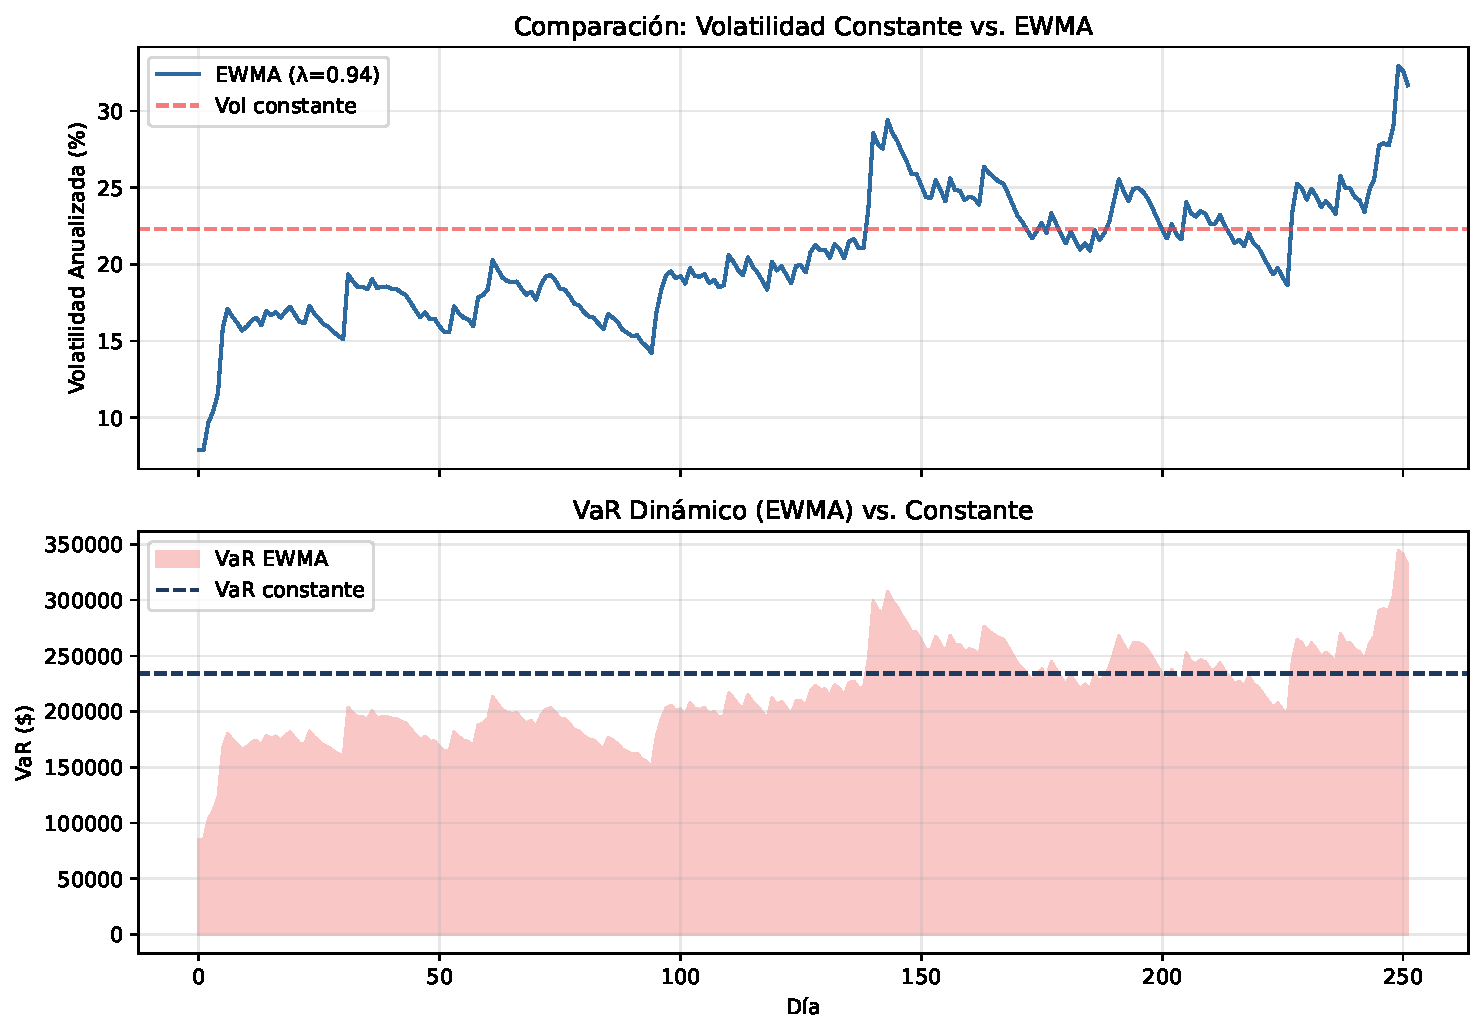
\includegraphics[keepaspectratio]{unidad3/cap11_var_expected_shortfall_files/figure-pdf/ewma-output-1.pdf}}

Leé los dos paneles juntos. Arriba: la volatilidad EWMA oscila alrededor
de la constante (línea roja), con episodios donde se dispara por encima
y períodos donde duerme por debajo --- la línea roja es el promedio de
dos regímenes distintos. Abajo, la consecuencia para el riesgo: el
\textbf{VaR dinámico se expande en los períodos agitados y se contrae en
los tranquilos}, mientras el VaR constante ignora todo. En los picos, el
VaR constante está \emph{subestimando} el riesgo del día --- y esas son
exactamente las excepciones agrupadas que el test de Kupiec no sabe
detectar.

\begin{center}\rule{0.5\linewidth}{0.5pt}\end{center}

\chapter{Test de Normalidad}\label{test-de-normalidad}

Cerramos auditando el supuesto sobre el que descansa todo el enfoque
paramétrico: ¿los retornos son normales? El \textbf{test de Jarque-Bera}
lo contrasta midiendo asimetría y curtosis:

\begin{itemize}
\tightlist
\item
  \(H_0\): Los retornos son normales (skewness = 0, curtosis = 3)
\item
  \(H_1\): No son normales
\end{itemize}

\phantomsection\label{normalidad}
\begin{Shaded}
\begin{Highlighting}[]
\ImportTok{from}\NormalTok{ scipy.stats }\ImportTok{import}\NormalTok{ jarque\_bera, skew, kurtosis}

\NormalTok{jb\_stat, jb\_pvalue }\OperatorTok{=}\NormalTok{ jarque\_bera(retornos)}
\NormalTok{s }\OperatorTok{=}\NormalTok{ skew(retornos)}
\NormalTok{k }\OperatorTok{=}\NormalTok{ kurtosis(retornos, fisher}\OperatorTok{=}\VariableTok{True}\NormalTok{)  }\CommentTok{\# Exceso de curtosis}

\BuiltInTok{print}\NormalTok{(}\SpecialStringTok{f"Skewness (asimetría):    }\SpecialCharTok{\{}\NormalTok{s}\SpecialCharTok{:\textgreater{}+.4f\}}\SpecialStringTok{  (normal = 0)"}\NormalTok{)}
\BuiltInTok{print}\NormalTok{(}\SpecialStringTok{f"Exc. Curtosis:           }\SpecialCharTok{\{}\NormalTok{k}\SpecialCharTok{:\textgreater{}+.4f\}}\SpecialStringTok{  (normal = 0)"}\NormalTok{)}
\BuiltInTok{print}\NormalTok{(}\SpecialStringTok{f"Jarque{-}Bera stat:        }\SpecialCharTok{\{}\NormalTok{jb\_stat}\SpecialCharTok{:\textgreater{}.4f\}}\SpecialStringTok{"}\NormalTok{)}
\BuiltInTok{print}\NormalTok{(}\SpecialStringTok{f"p{-}value:                 }\SpecialCharTok{\{}\NormalTok{jb\_pvalue}\SpecialCharTok{:\textgreater{}.4f\}}\SpecialStringTok{"}\NormalTok{)}
\BuiltInTok{print}\NormalTok{(}\SpecialStringTok{f"}\SpecialCharTok{\{}\StringTok{\textquotesingle{}{-}\textgreater{} No se rechaza normalidad\textquotesingle{}} \ControlFlowTok{if}\NormalTok{ jb\_pvalue }\OperatorTok{\textgreater{}} \FloatTok{0.05} \ControlFlowTok{else} \StringTok{\textquotesingle{}{-}\textgreater{} Se rechaza normalidad\textquotesingle{}}\SpecialCharTok{\}}\SpecialStringTok{"}\NormalTok{)}
\end{Highlighting}
\end{Shaded}

\begin{verbatim}
Skewness (asimetría):    +0.3848  (normal = 0)
Exc. Curtosis:           +0.1543  (normal = 0)
Jarque-Bera stat:        6.4692
p-value:                 0.0394
-> Se rechaza normalidad
\end{verbatim}

El test no rechaza --- pero ojo con la lectura: nuestros retornos
\textbf{fueron simulados de una normal}, así que el test está
funcionando como debe (no encuentra anormalidad donde no la hay). El
valor pedagógico está en el contraste con lo que pasa al aplicar
exactamente este test a datos reales:

\begin{tcolorbox}[enhanced jigsaw, bottomrule=.15mm, colback=white, opacitybacktitle=0.6, arc=.35mm, toprule=.15mm, opacityback=0, breakable, titlerule=0mm, left=2mm, coltitle=black, colbacktitle=quarto-callout-warning-color!10!white, colframe=quarto-callout-warning-color-frame, leftrule=.75mm, toptitle=1mm, bottomtitle=1mm, title=\textcolor{quarto-callout-warning-color}{\faExclamationTriangle}\hspace{0.5em}{En datos reales\ldots{}}, rightrule=.15mm]

Los retornos financieros reales típicamente \textbf{rechazan} la
normalidad con p-values microscópicos. Presentan:

\begin{itemize}
\tightlist
\item
  \textbf{Curtosis excesiva} (colas pesadas → más eventos extremos que
  la normal)
\item
  \textbf{Asimetría negativa} (más crashes que rallies)
\end{itemize}

Esto hace que el VaR paramétrico normal \textbf{subestime} el riesgo
verdadero --- especialmente al 99\%, donde manda la cola. Es el motivo
de fondo por el que existen el VaR histórico, el ES, y los modelos con
saltos del Capítulo 14.

\end{tcolorbox}

\begin{center}\rule{0.5\linewidth}{0.5pt}\end{center}

\chapter{Resumen de Métricas}\label{resumen-de-muxe9tricas}

\phantomsection\label{resumen}
\begin{Shaded}
\begin{Highlighting}[]
\ImportTok{import}\NormalTok{ pandas }\ImportTok{as}\NormalTok{ pd}

\NormalTok{resumen }\OperatorTok{=}\NormalTok{ pd.DataFrame(\{}
    \StringTok{"Métrica"}\NormalTok{: [}\StringTok{"VaR Paramétrico 95\%"}\NormalTok{, }\StringTok{"VaR Paramétrico 99\%"}\NormalTok{, }
                \StringTok{"VaR Histórico 95\%"}\NormalTok{, }\StringTok{"VaR Histórico 99\%"}\NormalTok{,}
                \StringTok{"CVaR 95\%"}\NormalTok{, }\StringTok{"CVaR 99\%"}\NormalTok{],}
    \StringTok{"Valor ($)"}\NormalTok{: [var\_param\_95, var\_param\_99, var\_hist\_95, var\_hist\_99, }
\NormalTok{                  cvar\_95, cvar\_99],}
    \StringTok{"\% Portafolio"}\NormalTok{: [var\_param\_95}\OperatorTok{/}\NormalTok{valor\_portafolio, var\_param\_99}\OperatorTok{/}\NormalTok{valor\_portafolio,}
\NormalTok{                     var\_hist\_95}\OperatorTok{/}\NormalTok{valor\_portafolio, var\_hist\_99}\OperatorTok{/}\NormalTok{valor\_portafolio,}
\NormalTok{                     cvar\_95}\OperatorTok{/}\NormalTok{valor\_portafolio, cvar\_99}\OperatorTok{/}\NormalTok{valor\_portafolio],}
\NormalTok{\})}

\NormalTok{resumen[}\StringTok{"Valor ($)"}\NormalTok{] }\OperatorTok{=}\NormalTok{ resumen[}\StringTok{"Valor ($)"}\NormalTok{].}\BuiltInTok{apply}\NormalTok{(}\KeywordTok{lambda}\NormalTok{ x: }\SpecialStringTok{f"$}\SpecialCharTok{\{}\NormalTok{x}\SpecialCharTok{:,.2f\}}\SpecialStringTok{"}\NormalTok{)}
\NormalTok{resumen[}\StringTok{"\% Portafolio"}\NormalTok{] }\OperatorTok{=}\NormalTok{ resumen[}\StringTok{"\% Portafolio"}\NormalTok{].}\BuiltInTok{apply}\NormalTok{(}\KeywordTok{lambda}\NormalTok{ x: }\SpecialStringTok{f"}\SpecialCharTok{\{}\NormalTok{x}\SpecialCharTok{:.4\%\}}\SpecialStringTok{"}\NormalTok{)}

\BuiltInTok{print}\NormalTok{(resumen.to\_string(index}\OperatorTok{=}\VariableTok{False}\NormalTok{))}
\end{Highlighting}
\end{Shaded}

\begin{verbatim}
            Métrica   Valor ($) % Portafolio
VaR Paramétrico 95% $234,134.38      2.3413%
VaR Paramétrico 99% $329,791.90      3.2979%
  VaR Histórico 95% $213,744.80      2.1374%
  VaR Histórico 99% $295,941.84      2.9594%
           CVaR 95% $257,564.55      2.5756%
           CVaR 99% $312,475.37      3.1248%
\end{verbatim}

\begin{center}\rule{0.5\linewidth}{0.5pt}\end{center}

\chapter{Con datos reales}\label{con-datos-reales-2}

El capítulo entero descansó sobre retornos simulados de una normal ---
ideal para aprender los métodos, tramposo para juzgarlos. El veredicto
final se lo damos a los datos: cinco años del ETF SPY (el S\&P 500), del
dataset del libro (\texttt{datos/precios.csv}, ver
Apéndice~\ref{sec-datos-financieros}).

\phantomsection\label{var-datos-reales}
\begin{Shaded}
\begin{Highlighting}[]
\NormalTok{precios }\OperatorTok{=}\NormalTok{ pd.read\_csv(}\StringTok{"../datos/precios.csv"}\NormalTok{, index\_col}\OperatorTok{=}\StringTok{"Date"}\NormalTok{, parse\_dates}\OperatorTok{=}\VariableTok{True}\NormalTok{)}
\NormalTok{r\_spy }\OperatorTok{=}\NormalTok{ precios[}\StringTok{"SPY"}\NormalTok{].pct\_change().dropna().values}

\NormalTok{mu\_spy, sigma\_spy }\OperatorTok{=}\NormalTok{ r\_spy.mean(), r\_spy.std()}
\NormalTok{p5, p1 }\OperatorTok{=}\NormalTok{ np.percentile(r\_spy, }\DecValTok{5}\NormalTok{), np.percentile(r\_spy, }\DecValTok{1}\NormalTok{)}

\BuiltInTok{print}\NormalTok{(}\SpecialStringTok{f"SPY: }\SpecialCharTok{\{}\BuiltInTok{len}\NormalTok{(r\_spy)}\SpecialCharTok{\}}\SpecialStringTok{ ruedas (}\SpecialCharTok{\{}\NormalTok{precios}\SpecialCharTok{.}\NormalTok{index[}\DecValTok{0}\NormalTok{]}\SpecialCharTok{:}\OperatorTok{\%}\NormalTok{Y}\OperatorTok{{-}\%}\NormalTok{m}\SpecialCharTok{\}}\SpecialStringTok{ a }\SpecialCharTok{\{}\NormalTok{precios}\SpecialCharTok{.}\NormalTok{index[}\OperatorTok{{-}}\DecValTok{1}\NormalTok{]}\SpecialCharTok{:}\OperatorTok{\%}\NormalTok{Y}\OperatorTok{{-}\%}\NormalTok{m}\SpecialCharTok{\}}\SpecialStringTok{)}\CharTok{\textbackslash{}n}\SpecialStringTok{"}\NormalTok{)}
\BuiltInTok{print}\NormalTok{(}\SpecialStringTok{f"}\SpecialCharTok{\{}\StringTok{\textquotesingle{}\textquotesingle{}}\SpecialCharTok{:24\}\{}\StringTok{\textquotesingle{}95\%\textquotesingle{}}\SpecialCharTok{:\textgreater{}12\}\{}\StringTok{\textquotesingle{}99\%\textquotesingle{}}\SpecialCharTok{:\textgreater{}12\}}\SpecialStringTok{"}\NormalTok{)}
\BuiltInTok{print}\NormalTok{(}\SpecialStringTok{f"}\SpecialCharTok{\{}\StringTok{\textquotesingle{}VaR paramétrico\textquotesingle{}}\SpecialCharTok{:\textless{}24\}}\SpecialStringTok{"}
      \SpecialStringTok{f"$}\SpecialCharTok{\{}\OperatorTok{{-}}\NormalTok{(mu\_spy }\OperatorTok{+}\NormalTok{ stats.norm.ppf(}\FloatTok{0.05}\NormalTok{) }\OperatorTok{*}\NormalTok{ sigma\_spy) }\OperatorTok{*}\NormalTok{ valor\_portafolio}\SpecialCharTok{:\textgreater{}11,.0f\}}\SpecialStringTok{"}
      \SpecialStringTok{f"$}\SpecialCharTok{\{}\OperatorTok{{-}}\NormalTok{(mu\_spy }\OperatorTok{+}\NormalTok{ stats.norm.ppf(}\FloatTok{0.01}\NormalTok{) }\OperatorTok{*}\NormalTok{ sigma\_spy) }\OperatorTok{*}\NormalTok{ valor\_portafolio}\SpecialCharTok{:\textgreater{}11,.0f\}}\SpecialStringTok{"}\NormalTok{)}
\BuiltInTok{print}\NormalTok{(}\SpecialStringTok{f"}\SpecialCharTok{\{}\StringTok{\textquotesingle{}VaR histórico\textquotesingle{}}\SpecialCharTok{:\textless{}24\}}\SpecialStringTok{"}
      \SpecialStringTok{f"$}\SpecialCharTok{\{}\OperatorTok{{-}}\NormalTok{p5 }\OperatorTok{*}\NormalTok{ valor\_portafolio}\SpecialCharTok{:\textgreater{}11,.0f\}}\SpecialStringTok{"}
      \SpecialStringTok{f"$}\SpecialCharTok{\{}\OperatorTok{{-}}\NormalTok{p1 }\OperatorTok{*}\NormalTok{ valor\_portafolio}\SpecialCharTok{:\textgreater{}11,.0f\}}\SpecialStringTok{"}\NormalTok{)}
\BuiltInTok{print}\NormalTok{(}\SpecialStringTok{f"}\SpecialCharTok{\{}\StringTok{\textquotesingle{}ES histórico\textquotesingle{}}\SpecialCharTok{:\textless{}24\}}\SpecialStringTok{"}
      \SpecialStringTok{f"$}\SpecialCharTok{\{}\OperatorTok{{-}}\NormalTok{r\_spy[r\_spy }\OperatorTok{\textless{}}\NormalTok{ p5]}\SpecialCharTok{.}\NormalTok{mean() }\OperatorTok{*}\NormalTok{ valor\_portafolio}\SpecialCharTok{:\textgreater{}11,.0f\}}\SpecialStringTok{"}
      \SpecialStringTok{f"$}\SpecialCharTok{\{}\OperatorTok{{-}}\NormalTok{r\_spy[r\_spy }\OperatorTok{\textless{}}\NormalTok{ p1]}\SpecialCharTok{.}\NormalTok{mean() }\OperatorTok{*}\NormalTok{ valor\_portafolio}\SpecialCharTok{:\textgreater{}11,.0f\}}\SpecialStringTok{"}\NormalTok{)}

\NormalTok{jb\_r, jb\_p }\OperatorTok{=}\NormalTok{ jarque\_bera(r\_spy)}
\BuiltInTok{print}\NormalTok{(}\SpecialStringTok{f"}\CharTok{\textbackslash{}n}\SpecialStringTok{Jarque{-}Bera: estadístico }\SpecialCharTok{\{}\NormalTok{jb\_r}\SpecialCharTok{:,.0f\}}\SpecialStringTok{, p{-}value }\SpecialCharTok{\{}\NormalTok{jb\_p}\SpecialCharTok{:.2e\}}\SpecialStringTok{"}\NormalTok{)}
\BuiltInTok{print}\NormalTok{(}\SpecialStringTok{f"Exceso de curtosis: }\SpecialCharTok{\{}\NormalTok{kurtosis(r\_spy, fisher}\OperatorTok{=}\VariableTok{True}\NormalTok{)}\SpecialCharTok{:+.2f\}}\SpecialStringTok{ | "}
      \SpecialStringTok{f"Asimetría: }\SpecialCharTok{\{}\NormalTok{skew(r\_spy)}\SpecialCharTok{:+.2f\}}\SpecialStringTok{"}\NormalTok{)}
\end{Highlighting}
\end{Shaded}

\begin{verbatim}
SPY: 1252 ruedas (2021-07 a 2026-06)

                                 95%         99%
VaR paramétrico         $    172,498$    246,231
VaR histórico           $    166,301$    292,978
ES histórico            $    246,686$    387,806

Jarque-Bera: estadístico 4,213, p-value 0.00e+00
Exceso de curtosis: +8.97 | Asimetría: +0.31
\end{verbatim}

Todo lo que el capítulo anticipó, junto y en un solo resultado. Al 95\%,
el paramétrico y el histórico casi coinciden --- a esa profundidad de la
cola, la normal todavía zafa. Al \textbf{99\% se separan}: los peores
días reales del S\&P son peores de lo que la campana admite, y el
histórico lo reporta. El ES amplifica el mensaje (la cola no solo
empieza antes: es más profunda). Y el test de Jarque-Bera, que con los
datos simulados no encontraba nada, acá \textbf{rechaza la normalidad
sin despeinarse} --- el exceso de curtosis positivo es la firma de las
colas pesadas. Con datos reales, el VaR paramétrico normal es la métrica
que menos deberías creerle justo donde más la necesitás.

\begin{center}\rule{0.5\linewidth}{0.5pt}\end{center}

\chapter{Errores comunes}\label{errores-comunes-9}

\begin{tcolorbox}[enhanced jigsaw, bottomrule=.15mm, colback=white, opacitybacktitle=0.6, arc=.35mm, toprule=.15mm, opacityback=0, breakable, titlerule=0mm, left=2mm, coltitle=black, colbacktitle=quarto-callout-warning-color!10!white, colframe=quarto-callout-warning-color-frame, leftrule=.75mm, toptitle=1mm, bottomtitle=1mm, title=\textcolor{quarto-callout-warning-color}{\faExclamationTriangle}\hspace{0.5em}{Trampas frecuentes}, rightrule=.15mm]

\begin{itemize}
\tightlist
\item
  \textbf{El signo del cuantil}: el percentil 5 de los retornos es un
  número \emph{negativo}; el VaR se reporta \emph{positivo} (es una
  pérdida). Ese signo menos perdido es el bug más común en
  implementaciones de VaR --- verificá que tu VaR sea positivo.
\item
  \textbf{Escalar con \(\sqrt{t}\) sin pensar}:
  \(VaR_{10d} = VaR_{1d}\sqrt{10}\) solo vale si los retornos son i.i.d.
  y sin autocorrelación. Con volatility clustering (o sea, siempre), la
  regla subestima el riesgo de horizontes largos en épocas agitadas.
\item
  \textbf{Confundir VaR en \% con VaR en \$}: mezclar las dos unidades a
  mitad de un cálculo (multiplicar dos veces por \(W\), o ninguna)
  produce errores de orden de magnitud que a veces sobreviven hasta el
  reporte.
\item
  \textbf{Volatilidad sin anualizar (o anualizada dos veces)}: sé
  consistente con el horizonte --- VaR diario con \(\sigma\) diaria, VaR
  anual con \(\sigma\) anual. La mezcla es otro clásico silencioso.
\item
  \textbf{Auditar solo la cantidad de excepciones}: Kupiec aprueba un
  modelo cuyas excepciones vienen todas juntas en una crisis. Mirá
  también \emph{cuándo} ocurren (independencia), no solo cuántas son.
\end{itemize}

\end{tcolorbox}

\begin{center}\rule{0.5\linewidth}{0.5pt}\end{center}

\chapter{Ejercicios Propuestos}\label{ejercicios-propuestos-10}

\begin{tcolorbox}[enhanced jigsaw, bottomrule=.15mm, colback=white, opacitybacktitle=0.6, arc=.35mm, toprule=.15mm, opacityback=0, breakable, titlerule=0mm, left=2mm, coltitle=black, colbacktitle=quarto-callout-important-color!10!white, colframe=quarto-callout-important-color-frame, leftrule=.75mm, toptitle=1mm, bottomtitle=1mm, title=\textcolor{quarto-callout-important-color}{\faExclamation}\hspace{0.5em}{Ejercicios}, rightrule=.15mm]

\begin{enumerate}
\def\labelenumi{\arabic{enumi}.}
\item
  \textbf{VaR a 10 días}: Escalar el VaR diario a 10 días usando la
  regla de la raíz cuadrada: \(VaR_{10d} = VaR_{1d} \times \sqrt{10}\).
  ¿Es válida esta aproximación? ¿Bajo qué supuestos?
\item
  \textbf{Backtesting rolling}: Implementar un backtesting con ventana
  móvil de 60 días. Graficar la tasa de excepciones a lo largo del
  tiempo.
\item
  \textbf{VaR con distribución t-Student}: Reemplazar la distribución
  normal por una t-Student con \texttt{df} grados de libertad estimados
  de los datos. Comparar con el VaR normal.
\item
  \textbf{Stress testing}: Calcular el VaR condicional asumiendo que la
  volatilidad se duplica (escenario de estrés). ¿Cuánto aumenta el VaR?
\end{enumerate}

\end{tcolorbox}

Podés resolver estos ejercicios acá mismo: la celda ejecuta Python
\textbf{en tu navegador}, sin instalar nada (la primera ejecución tarda
unos segundos mientras carga el entorno; los paquetes que importes se
instalan solos).

\begin{Shaded}
\begin{Highlighting}[]
\NormalTok{\#| label: practica{-}navegador}
\NormalTok{import numpy as np}
\NormalTok{from scipy import stats}

\NormalTok{\# Para usar el dataset real del libro (requiere conexión):}
\NormalTok{\# import pandas as pd}
\NormalTok{\# from pyodide.http import open\_url}
\NormalTok{\# url = "https://diegoonna.github.io/libro\_finanzas\_computacionales/datos/precios.csv"}
\NormalTok{\# precios = pd.read\_csv(open\_url(url), index\_col="Date", parse\_dates=True)}

\NormalTok{\# Tu solución acá...}
\end{Highlighting}
\end{Shaded}

\begin{center}\rule{0.5\linewidth}{0.5pt}\end{center}

\chapter{Referencias}\label{referencias-10}

\phantomsection\label{refs}

\chapter{Capítulo 12: Riesgo y
Regulación}\label{capuxedtulo-12-riesgo-y-regulaciuxf3n}

Stress testing, Basilea III y las lecciones de las crisis

Las métricas del capítulo anterior no viven en el vacío: existen dentro
de un marco regulatorio construido, crisis tras crisis, sobre las ruinas
de modelos que fallaron. Recorremos el stress testing, la arquitectura
de Basilea III, el PPNR y la taxonomía de riesgos, y estudiamos en
detalle dos casos que todo analista cuantitativo debería conocer de
memoria: el colapso de LTCM (1998) y la crisis de 2008, con su
correlación falsa en el corazón.

\hfill\break

\chapter{Introducción}\label{introducciuxf3n-9}

En el capítulo anterior aprendimos a medir el riesgo con VaR y Expected
Shortfall. Este capítulo responde una pregunta distinta: \textbf{¿qué
pasa cuando los modelos fallan?} Porque fallan. Y cuando fallan a escala
de sistema financiero, las consecuencias las paga toda la economía.

La regulación bancaria moderna es, en gran medida, la \textbf{historia
acumulada de esos fracasos}: cada crisis dejó una regla nueva. Entender
ese marco no es un tema ``legal'' ajeno al análisis cuantitativo ---
define qué modelos se usan, cuánto capital inmovilizan los bancos y qué
límites tiene la toma de riesgo. Y las dos historias que cierran el
capítulo (LTCM y 2008) son las mejores clases de humildad cuantitativa
jamás dictadas.

\phantomsection\label{setup}
\begin{Shaded}
\begin{Highlighting}[]
\ImportTok{import}\NormalTok{ numpy }\ImportTok{as}\NormalTok{ np}
\ImportTok{import}\NormalTok{ pandas }\ImportTok{as}\NormalTok{ pd}
\ImportTok{import}\NormalTok{ matplotlib.pyplot }\ImportTok{as}\NormalTok{ plt}
\ImportTok{from}\NormalTok{ scipy }\ImportTok{import}\NormalTok{ stats}

\NormalTok{rng }\OperatorTok{=}\NormalTok{ np.random.default\_rng(}\DecValTok{42}\NormalTok{)}
\end{Highlighting}
\end{Shaded}

\begin{center}\rule{0.5\linewidth}{0.5pt}\end{center}

\chapter{Stress testing: preguntar ``¿y
si\ldots?''}\label{stress-testing-preguntar-y-si}

El VaR mira la distribución \emph{estimada con datos recientes}. El
\textbf{stress testing} hace la pregunta complementaria: \emph{¿cuánto
perdería la cartera si se repitiera un escenario extremo concreto?} No
pregunta por probabilidades --- pregunta por \textbf{consecuencias}.

Hay dos familias de escenarios:

\begin{itemize}
\tightlist
\item
  \textbf{Históricos}: replicar episodios reales (crash de 1987, crisis
  de 2008, COVID de marzo 2020) sobre la cartera actual.
\item
  \textbf{Hipotéticos}: construir escenarios que no ocurrieron pero
  podrían (``el petróleo cae 50\% y la tasa sube 300 puntos básicos'').
\end{itemize}

\phantomsection\label{stress-testing}
\begin{Shaded}
\begin{Highlighting}[]
\CommentTok{\# Una cartera simple: acciones, bonos y commodities}
\NormalTok{cartera }\OperatorTok{=}\NormalTok{ pd.Series(\{}\StringTok{"Acciones"}\NormalTok{: }\DecValTok{6\_000\_000}\NormalTok{, }\StringTok{"Bonos"}\NormalTok{: }\DecValTok{3\_000\_000}\NormalTok{, }\StringTok{"Commodities"}\NormalTok{: }\DecValTok{1\_000\_000}\NormalTok{\})}

\CommentTok{\# Escenarios de estrés: shock (\%) aplicado a cada clase de activo}
\NormalTok{escenarios }\OperatorTok{=}\NormalTok{ pd.DataFrame(\{}
    \StringTok{"Crash 1987"}\NormalTok{:        \{}\StringTok{"Acciones"}\NormalTok{: }\OperatorTok{{-}}\FloatTok{0.23}\NormalTok{, }\StringTok{"Bonos"}\NormalTok{: }\OperatorTok{+}\FloatTok{0.02}\NormalTok{, }\StringTok{"Commodities"}\NormalTok{: }\OperatorTok{{-}}\FloatTok{0.05}\NormalTok{\},}
    \StringTok{"Crisis 2008 (oct)"}\NormalTok{: \{}\StringTok{"Acciones"}\NormalTok{: }\OperatorTok{{-}}\FloatTok{0.17}\NormalTok{, }\StringTok{"Bonos"}\NormalTok{: }\OperatorTok{{-}}\FloatTok{0.05}\NormalTok{, }\StringTok{"Commodities"}\NormalTok{: }\OperatorTok{{-}}\FloatTok{0.20}\NormalTok{\},}
    \StringTok{"COVID mar{-}2020"}\NormalTok{:    \{}\StringTok{"Acciones"}\NormalTok{: }\OperatorTok{{-}}\FloatTok{0.12}\NormalTok{, }\StringTok{"Bonos"}\NormalTok{: }\OperatorTok{+}\FloatTok{0.01}\NormalTok{, }\StringTok{"Commodities"}\NormalTok{: }\OperatorTok{{-}}\FloatTok{0.25}\NormalTok{\},}
    \StringTok{"Suba de tasas"}\NormalTok{:     \{}\StringTok{"Acciones"}\NormalTok{: }\OperatorTok{{-}}\FloatTok{0.08}\NormalTok{, }\StringTok{"Bonos"}\NormalTok{: }\OperatorTok{{-}}\FloatTok{0.12}\NormalTok{, }\StringTok{"Commodities"}\NormalTok{: }\OperatorTok{+}\FloatTok{0.03}\NormalTok{\},}
\NormalTok{\}).T}

\NormalTok{perdidas }\OperatorTok{=}\NormalTok{ escenarios }\OperatorTok{@}\NormalTok{ cartera}

\BuiltInTok{print}\NormalTok{(}\SpecialStringTok{f"Cartera total: $}\SpecialCharTok{\{}\NormalTok{cartera}\SpecialCharTok{.}\BuiltInTok{sum}\NormalTok{()}\SpecialCharTok{:,.0f\}}\CharTok{\textbackslash{}n}\SpecialStringTok{"}\NormalTok{)}
\BuiltInTok{print}\NormalTok{(}\StringTok{"Pérdida por escenario de estrés:"}\NormalTok{)}
\ControlFlowTok{for}\NormalTok{ esc, p }\KeywordTok{in}\NormalTok{ perdidas.items():}
    \BuiltInTok{print}\NormalTok{(}\SpecialStringTok{f"  }\SpecialCharTok{\{}\NormalTok{esc}\SpecialCharTok{:\textless{}18\}}\SpecialStringTok{ $}\SpecialCharTok{\{}\NormalTok{p}\SpecialCharTok{:\textgreater{}12,.0f\}}\SpecialStringTok{  (}\SpecialCharTok{\{}\NormalTok{p }\OperatorTok{/}\NormalTok{ cartera}\SpecialCharTok{.}\BuiltInTok{sum}\NormalTok{()}\SpecialCharTok{:\textgreater{}6.1\%\}}\SpecialStringTok{)"}\NormalTok{)}
\end{Highlighting}
\end{Shaded}

\begin{verbatim}
Cartera total: $10,000,000

Pérdida por escenario de estrés:
  Crash 1987         $  -1,370,000  (-13.7%)
  Crisis 2008 (oct)  $  -1,370,000  (-13.7%)
  COVID mar-2020     $    -940,000  ( -9.4%)
  Suba de tasas      $    -810,000  ( -8.1%)
\end{verbatim}

La tabla de arriba es, en miniatura, lo que los reguladores exigen a los
bancos a escala gigante: los \textbf{CCAR/DFAST} en EEUU y los stress
tests del BCE someten los balances completos a escenarios macro adversos
de varios años. Un banco que ``no aprueba'' enfrenta restricciones para
pagar dividendos o recomprar acciones.

\begin{tcolorbox}[enhanced jigsaw, bottomrule=.15mm, colback=white, opacitybacktitle=0.6, arc=.35mm, toprule=.15mm, opacityback=0, breakable, titlerule=0mm, left=2mm, coltitle=black, colbacktitle=quarto-callout-tip-color!10!white, colframe=quarto-callout-tip-color-frame, leftrule=.75mm, toptitle=1mm, bottomtitle=1mm, title=\textcolor{quarto-callout-tip-color}{\faLightbulb}\hspace{0.5em}{VaR y stress testing se complementan}, rightrule=.15mm]

El VaR dice \emph{``esto es lo que puede pasar en un día normal-malo,
según los datos recientes''}. El stress test dice \emph{``esto es lo que
pasaría si vuelve 2008, tengan los datos recientes la pinta que
tengan''}. El primero es probabilístico y miope; el segundo es
determinístico y de memoria larga. Un buen tablero de riesgo muestra
ambos.

\end{tcolorbox}

\begin{center}\rule{0.5\linewidth}{0.5pt}\end{center}

\chapter{Basilea III: la arquitectura
regulatoria}\label{basilea-iii-la-arquitectura-regulatoria}

Los \textbf{Acuerdos de Basilea} son los estándares globales de
regulación bancaria, emitidos por el Comité de Basilea (BIS). La versión
III, respuesta directa a 2008, se apoya en tres pilares conceptuales:
capital de mejor calidad, límites al apalancamiento y ---por primera
vez--- reglas de liquidez.

\section{Capital: el colchón contra
pérdidas}\label{capital-el-colchuxf3n-contra-puxe9rdidas}

La idea central: los activos de un banco pueden perder valor; el
\textbf{capital propio} es el colchón que absorbe esas pérdidas antes de
que las paguen los depositantes. Basilea exige un mínimo de capital
\textbf{en proporción al riesgo de los activos}:

\[\text{Ratio de capital} = \frac{\text{Capital}}{\text{RWA}} \geq \text{mínimos regulatorios}\]

donde \textbf{RWA} (\emph{Risk-Weighted Assets}) son los activos
ponderados por riesgo: un bono del tesoro pondera cerca de 0\%, una
hipoteca \textasciitilde35-50\%, un préstamo corporativo riesgoso 100\%
o más. Mil millones en letras del tesoro exigen mucho menos capital que
mil millones en préstamos a startups --- razonable.

\phantomsection\label{rwa}
\begin{Shaded}
\begin{Highlighting}[]
\CommentTok{\# Balance simplificado de un banco}
\NormalTok{activos }\OperatorTok{=}\NormalTok{ pd.DataFrame(\{}
    \StringTok{"monto"}\NormalTok{:       [}\DecValTok{400}\NormalTok{, }\DecValTok{300}\NormalTok{, }\DecValTok{200}\NormalTok{, }\DecValTok{100}\NormalTok{],     }\CommentTok{\# en millones}
    \StringTok{"ponderacion"}\NormalTok{: [}\FloatTok{0.00}\NormalTok{, }\FloatTok{0.35}\NormalTok{, }\FloatTok{0.75}\NormalTok{, }\FloatTok{1.00}\NormalTok{], }\CommentTok{\# peso por riesgo (Basilea, aprox.)}
\NormalTok{\}, index}\OperatorTok{=}\NormalTok{[}\StringTok{"Bonos soberanos"}\NormalTok{, }\StringTok{"Hipotecas"}\NormalTok{, }\StringTok{"Préstamos PyME"}\NormalTok{, }\StringTok{"Préstamos corporativos"}\NormalTok{])}

\NormalTok{activos[}\StringTok{"RWA"}\NormalTok{] }\OperatorTok{=}\NormalTok{ activos[}\StringTok{"monto"}\NormalTok{] }\OperatorTok{*}\NormalTok{ activos[}\StringTok{"ponderacion"}\NormalTok{]}

\NormalTok{capital }\OperatorTok{=} \DecValTok{60}  \CommentTok{\# millones de capital CET1}

\BuiltInTok{print}\NormalTok{(activos)}
\BuiltInTok{print}\NormalTok{(}\SpecialStringTok{f"}\CharTok{\textbackslash{}n}\SpecialStringTok{Activos totales:  $}\SpecialCharTok{\{}\NormalTok{activos[}\StringTok{\textquotesingle{}monto\textquotesingle{}}\NormalTok{]}\SpecialCharTok{.}\BuiltInTok{sum}\NormalTok{()}\SpecialCharTok{:,.0f\}}\SpecialStringTok{M"}\NormalTok{)}
\BuiltInTok{print}\NormalTok{(}\SpecialStringTok{f"RWA totales:      $}\SpecialCharTok{\{}\NormalTok{activos[}\StringTok{\textquotesingle{}RWA\textquotesingle{}}\NormalTok{]}\SpecialCharTok{.}\BuiltInTok{sum}\NormalTok{()}\SpecialCharTok{:,.0f\}}\SpecialStringTok{M"}\NormalTok{)}
\BuiltInTok{print}\NormalTok{(}\SpecialStringTok{f"Ratio CET1:       }\SpecialCharTok{\{}\NormalTok{capital }\OperatorTok{/}\NormalTok{ activos[}\StringTok{\textquotesingle{}RWA\textquotesingle{}}\NormalTok{]}\SpecialCharTok{.}\BuiltInTok{sum}\NormalTok{()}\SpecialCharTok{:.1\%\}}\SpecialStringTok{  (mínimo con colchones: \textasciitilde{}10.5\%)"}\NormalTok{)}
\BuiltInTok{print}\NormalTok{(}\SpecialStringTok{f"Ratio de apalancamiento: }\SpecialCharTok{\{}\NormalTok{capital }\OperatorTok{/}\NormalTok{ activos[}\StringTok{\textquotesingle{}monto\textquotesingle{}}\NormalTok{]}\SpecialCharTok{.}\BuiltInTok{sum}\NormalTok{()}\SpecialCharTok{:.1\%\}}\SpecialStringTok{  (mínimo: 3\%)"}\NormalTok{)}
\end{Highlighting}
\end{Shaded}

\begin{verbatim}
                        monto  ponderacion    RWA
Bonos soberanos           400         0.00    0.0
Hipotecas                 300         0.35  105.0
Préstamos PyME            200         0.75  150.0
Préstamos corporativos    100         1.00  100.0

Activos totales:  $1,000M
RWA totales:      $355M
Ratio CET1:       16.9%  (mínimo con colchones: ~10.5%)
Ratio de apalancamiento: 6.0%  (mínimo: 3%)
\end{verbatim}

Fijate el contraste entre los dos ratios finales: el de capital usa RWA
(sensible al riesgo), el de \textbf{apalancamiento} usa activos totales
sin ponderar. Basilea III agregó el segundo justamente porque en 2008
varios bancos lucían ratios de capital sólidos\ldots{} calculados sobre
RWA que subestimaban el riesgo real.

\section{Liquidez: sobrevivir a la
corrida}\label{liquidez-sobrevivir-a-la-corrida}

2008 demostró que un banco puede ser \emph{solvente} y morir igual por
\emph{iliquidez}: si el fondeo de corto plazo desaparece de un día para
otro, no hay capital que alcance. Basilea III introdujo dos ratios:

\begin{itemize}
\tightlist
\item
  \textbf{LCR} (\emph{Liquidity Coverage Ratio}): tener activos líquidos
  de alta calidad suficientes para sobrevivir \textbf{30 días} de fuga
  de depósitos y fondeo.
\item
  \textbf{NSFR} (\emph{Net Stable Funding Ratio}): que los activos de
  largo plazo estén fondeados con pasivos estables, no con deuda que
  vence mañana.
\end{itemize}

\section{PPNR: la otra mitad del stress
test}\label{ppnr-la-otra-mitad-del-stress-test}

En los stress tests regulatorios, la pérdida de capital de un banco no
depende solo de cuánto pierden sus activos, sino de cuánto \textbf{sigue
ganando} su negocio durante la crisis. Esa capacidad de generar
resultados se proyecta con el \textbf{PPNR} (\emph{Pre-Provision Net
Revenue}): ingresos netos por intereses + comisiones − gastos
operativos, \textbf{antes} de provisiones por incobrables.

\[\Delta \text{Capital} \approx \text{PPNR} - \text{Pérdidas crediticias} - \text{Pérdidas de trading} - \text{Impuestos y dividendos}\]

\begin{Shaded}
\begin{Highlighting}[]
\CommentTok{\# Proyección estilizada a 9 trimestres (formato CCAR) bajo escenario adverso}
\NormalTok{trimestres }\OperatorTok{=}\NormalTok{ np.arange(}\DecValTok{1}\NormalTok{, }\DecValTok{10}\NormalTok{)}

\NormalTok{ppnr }\OperatorTok{=} \FloatTok{2.0} \OperatorTok{{-}} \FloatTok{0.15} \OperatorTok{*}\NormalTok{ trimestres            }\CommentTok{\# el negocio se deteriora gradualmente}
\NormalTok{perdidas\_credito }\OperatorTok{=} \FloatTok{1.0} \OperatorTok{+} \FloatTok{1.5} \OperatorTok{*}\NormalTok{ np.exp(}\OperatorTok{{-}}\FloatTok{0.5} \OperatorTok{*}\NormalTok{ (trimestres }\OperatorTok{{-}} \DecValTok{4}\NormalTok{) }\OperatorTok{**} \DecValTok{2} \OperatorTok{/} \DecValTok{4}\NormalTok{)  }\CommentTok{\# pico de mora}
\NormalTok{capital\_inicial }\OperatorTok{=} \DecValTok{60}

\NormalTok{capital }\OperatorTok{=}\NormalTok{ capital\_inicial }\OperatorTok{+}\NormalTok{ np.cumsum(ppnr }\OperatorTok{{-}}\NormalTok{ perdidas\_credito)}

\NormalTok{fig, ax }\OperatorTok{=}\NormalTok{ plt.subplots(figsize}\OperatorTok{=}\NormalTok{(}\DecValTok{9}\NormalTok{, }\FloatTok{4.5}\NormalTok{))}
\NormalTok{ax.plot(trimestres, capital, }\StringTok{"o{-}"}\NormalTok{, linewidth}\OperatorTok{=}\DecValTok{2}\NormalTok{, label}\OperatorTok{=}\StringTok{"Capital proyectado"}\NormalTok{)}
\NormalTok{ax.axhline(}\DecValTok{45}\NormalTok{, color}\OperatorTok{=}\StringTok{"red"}\NormalTok{, linestyle}\OperatorTok{=}\StringTok{"{-}{-}"}\NormalTok{, label}\OperatorTok{=}\StringTok{"Mínimo regulatorio (ilustrativo)"}\NormalTok{)}
\NormalTok{ax.fill\_between(trimestres, }\DecValTok{0}\NormalTok{, ppnr }\OperatorTok{*} \DecValTok{10}\NormalTok{, alpha}\OperatorTok{=}\FloatTok{0.15}\NormalTok{, color}\OperatorTok{=}\StringTok{"green"}\NormalTok{,}
\NormalTok{                label}\OperatorTok{=}\StringTok{"PPNR (escala ×10)"}\NormalTok{)}
\NormalTok{ax.set\_xlabel(}\StringTok{"Trimestre del escenario adverso"}\NormalTok{)}
\NormalTok{ax.set\_ylabel(}\StringTok{"Capital ($M)"}\NormalTok{)}
\NormalTok{ax.set\_title(}\StringTok{"Anatomía de un stress test: el PPNR amortigua las pérdidas"}\NormalTok{)}
\NormalTok{ax.legend()}
\NormalTok{ax.grid(}\VariableTok{True}\NormalTok{, alpha}\OperatorTok{=}\FloatTok{0.3}\NormalTok{)}
\NormalTok{plt.tight\_layout()}
\NormalTok{plt.show()}
\end{Highlighting}
\end{Shaded}

\pandocbounded{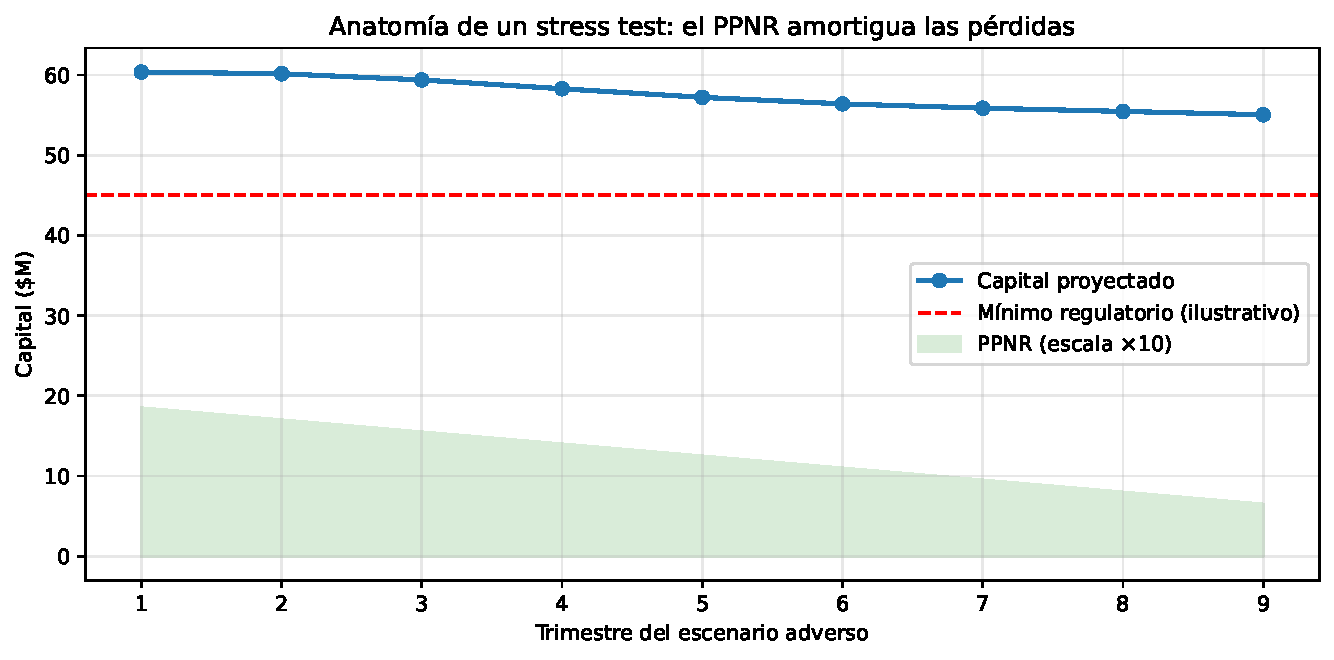
\includegraphics[keepaspectratio]{unidad3/cap12_riesgo_regulacion_files/figure-pdf/ppnr-output-1.pdf}}

La lección del gráfico: un banco con PPNR robusto puede absorber una ola
de pérdidas crediticias sin acercarse al mínimo; uno con PPNR débil
llega a la misma crisis sin amortiguador. Por eso los equipos de PPNR de
los bancos grandes emplean pequeños ejércitos de modeladores.

\section{Riesgo de mercado vs.~riesgo
operacional}\label{riesgo-de-mercado-vs.-riesgo-operacional}

Basilea clasifica los riesgos en tres grandes categorías, cada una con
su carga de capital:

\begin{longtable}[]{@{}
  >{\raggedright\arraybackslash}p{(\linewidth - 6\tabcolsep) * \real{0.2500}}
  >{\raggedright\arraybackslash}p{(\linewidth - 6\tabcolsep) * \real{0.2500}}
  >{\raggedright\arraybackslash}p{(\linewidth - 6\tabcolsep) * \real{0.2500}}
  >{\raggedright\arraybackslash}p{(\linewidth - 6\tabcolsep) * \real{0.2500}}@{}}
\toprule\noalign{}
\begin{minipage}[b]{\linewidth}\raggedright
Riesgo
\end{minipage} & \begin{minipage}[b]{\linewidth}\raggedright
Qué es
\end{minipage} & \begin{minipage}[b]{\linewidth}\raggedright
Ejemplo
\end{minipage} & \begin{minipage}[b]{\linewidth}\raggedright
Herramienta típica
\end{minipage} \\
\midrule\noalign{}
\endhead
\bottomrule\noalign{}
\endlastfoot
\textbf{De crédito} & La contraparte no paga & Mora hipotecaria &
PD/LGD/EAD, provisiones \\
\textbf{De mercado} & Los precios se mueven en contra & Caída del
portafolio de trading & VaR, ES (FRTB) \\
\textbf{Operacional} & Fallas de procesos, sistemas, personas & Fraude,
cyberataque, \emph{fat finger} & Bases de eventos, escenarios \\
\end{longtable}

El riesgo \textbf{operacional} es el más resbaladizo: no tiene
``posición'' que cerrar ni distribución de mercado que estimar. Casos
célebres: Barings (1995, un solo trader ocultando pérdidas quebró un
banco de 233 años), Société Générale (2008, €4.9bn), Knight Capital
(2012, un deploy de software defectuoso perdió \$440M en 45 minutos). Su
gestión es más de procesos y controles que de matemática --- pero su
carga de capital es real.

\begin{center}\rule{0.5\linewidth}{0.5pt}\end{center}

\chapter{Caso 1 --- LTCM: cuando los genios
fallan}\label{caso-1-ltcm-cuando-los-genios-fallan}

\textbf{Long-Term Capital Management} era, en 1997, el hedge fund más
prestigioso del planeta: fundado por el legendario trader John
Meriwether, con \textbf{Myron Scholes y Robert Merton} (Nobel 1997, los
del modelo de opciones) en el directorio. Su estrategia:
\emph{convergence trades} --- apostar a que diferenciales de precio
entre bonos casi idénticos (por ejemplo, un bono del tesoro recién
emitido contra uno viejo) se achicarían. Diferenciales minúsculos, así
que para volverlos rentables usaban un \textbf{apalancamiento de
\textasciitilde25:1}: con \$4.7bn de capital controlaban más de \$125bn
en posiciones.

Los modelos decían que esas posiciones eran seguras: los diferenciales
\emph{siempre} convergían, y las posiciones estaban diversificadas entre
mercados supuestamente independientes.

En agosto de 1998, \textbf{Rusia defaulteó su deuda}. Y ocurrió lo que
los modelos no contemplaban: en la corrida global hacia la calidad,
\emph{todos} los diferenciales se ampliaron \emph{a la vez}. Posiciones
``independientes'' en Japón, Europa y EEUU perdieron juntas: la
correlación, que en los datos históricos era baja, \textbf{saltó hacia 1
exactamente cuando importaba}. Con 25:1 de apalancamiento, no hay margen
para esperar la convergencia: los margin calls obligan a vender en el
peor momento, ampliando aún más los diferenciales --- una espiral. En
pocas semanas LTCM perdió \$4.4bn, y la Fed de Nueva York tuvo que
coordinar un rescate privado para evitar que la liquidación forzada
arrastrara al sistema.

\begin{Shaded}
\begin{Highlighting}[]
\CommentTok{\# La mecánica de LTCM en miniatura: apalancamiento + correlaciones que saltan}
\NormalTok{n\_dias }\OperatorTok{=} \DecValTok{250}
\NormalTok{n\_estrategias }\OperatorTok{=} \DecValTok{10}          \CommentTok{\# "apuestas independientes" de convergencia}
\NormalTok{apalancamiento }\OperatorTok{=} \DecValTok{25}

\CommentTok{\# Días normales: estrategias casi independientes (correlación 0.1), retorno positivo chico}
\CommentTok{\# Crisis (día 150 en adelante): correlación 0.9 y drift negativo}
\KeywordTok{def}\NormalTok{ simular\_pnl(rho, mu\_d, n\_dias, n\_est, rng):}
\NormalTok{    L }\OperatorTok{=}\NormalTok{ np.linalg.cholesky(np.full((n\_est, n\_est), rho) }\OperatorTok{+}\NormalTok{ (}\DecValTok{1} \OperatorTok{{-}}\NormalTok{ rho) }\OperatorTok{*}\NormalTok{ np.eye(n\_est))}
\NormalTok{    shocks }\OperatorTok{=}\NormalTok{ rng.standard\_normal((n\_dias, n\_est)) }\OperatorTok{@}\NormalTok{ L.T}
    \ControlFlowTok{return}\NormalTok{ mu\_d }\OperatorTok{+} \FloatTok{0.0015} \OperatorTok{*}\NormalTok{ shocks}

\NormalTok{pnl\_normal }\OperatorTok{=}\NormalTok{ simular\_pnl(}\FloatTok{0.10}\NormalTok{, }\OperatorTok{+}\FloatTok{0.0004}\NormalTok{, }\DecValTok{150}\NormalTok{, n\_estrategias, rng)}
\NormalTok{pnl\_crisis }\OperatorTok{=}\NormalTok{ simular\_pnl(}\FloatTok{0.90}\NormalTok{, }\OperatorTok{{-}}\FloatTok{0.0025}\NormalTok{, }\DecValTok{100}\NormalTok{, n\_estrategias, rng)}
\NormalTok{pnl\_total }\OperatorTok{=}\NormalTok{ np.vstack([pnl\_normal, pnl\_crisis]).mean(axis}\OperatorTok{=}\DecValTok{1}\NormalTok{)  }\CommentTok{\# cartera equiponderada}

\NormalTok{equity }\OperatorTok{=} \DecValTok{100} \OperatorTok{*}\NormalTok{ np.cumprod(}\DecValTok{1} \OperatorTok{+}\NormalTok{ apalancamiento }\OperatorTok{*}\NormalTok{ pnl\_total)}

\NormalTok{fig, ax }\OperatorTok{=}\NormalTok{ plt.subplots(figsize}\OperatorTok{=}\NormalTok{(}\DecValTok{9}\NormalTok{, }\FloatTok{4.5}\NormalTok{))}
\NormalTok{ax.plot(equity, linewidth}\OperatorTok{=}\DecValTok{2}\NormalTok{)}
\NormalTok{ax.axvline(}\DecValTok{150}\NormalTok{, color}\OperatorTok{=}\StringTok{"red"}\NormalTok{, linestyle}\OperatorTok{=}\StringTok{"{-}{-}"}\NormalTok{, label}\OperatorTok{=}\StringTok{"Default ruso: las correlaciones saltan"}\NormalTok{)}
\NormalTok{ax.set\_xlabel(}\StringTok{"Día"}\NormalTok{)}
\NormalTok{ax.set\_ylabel(}\StringTok{"Capital (base 100)"}\NormalTok{)}
\NormalTok{ax.set\_title(}\SpecialStringTok{f"LTCM estilizado: }\SpecialCharTok{\{}\NormalTok{n\_estrategias}\SpecialCharTok{\}}\SpecialStringTok{ apuestas \textquotesingle{}independientes\textquotesingle{} con apalancamiento }\SpecialCharTok{\{}\NormalTok{apalancamiento}\SpecialCharTok{\}}\SpecialStringTok{:1"}\NormalTok{)}
\NormalTok{ax.legend()}
\NormalTok{ax.grid(}\VariableTok{True}\NormalTok{, alpha}\OperatorTok{=}\FloatTok{0.3}\NormalTok{)}
\NormalTok{plt.tight\_layout()}
\NormalTok{plt.show()}

\BuiltInTok{print}\NormalTok{(}\SpecialStringTok{f"Capital final: }\SpecialCharTok{\{}\NormalTok{equity[}\OperatorTok{{-}}\DecValTok{1}\NormalTok{]}\SpecialCharTok{:.0f\}}\SpecialStringTok{ (arrancó en 100)"}\NormalTok{)}
\end{Highlighting}
\end{Shaded}

\pandocbounded{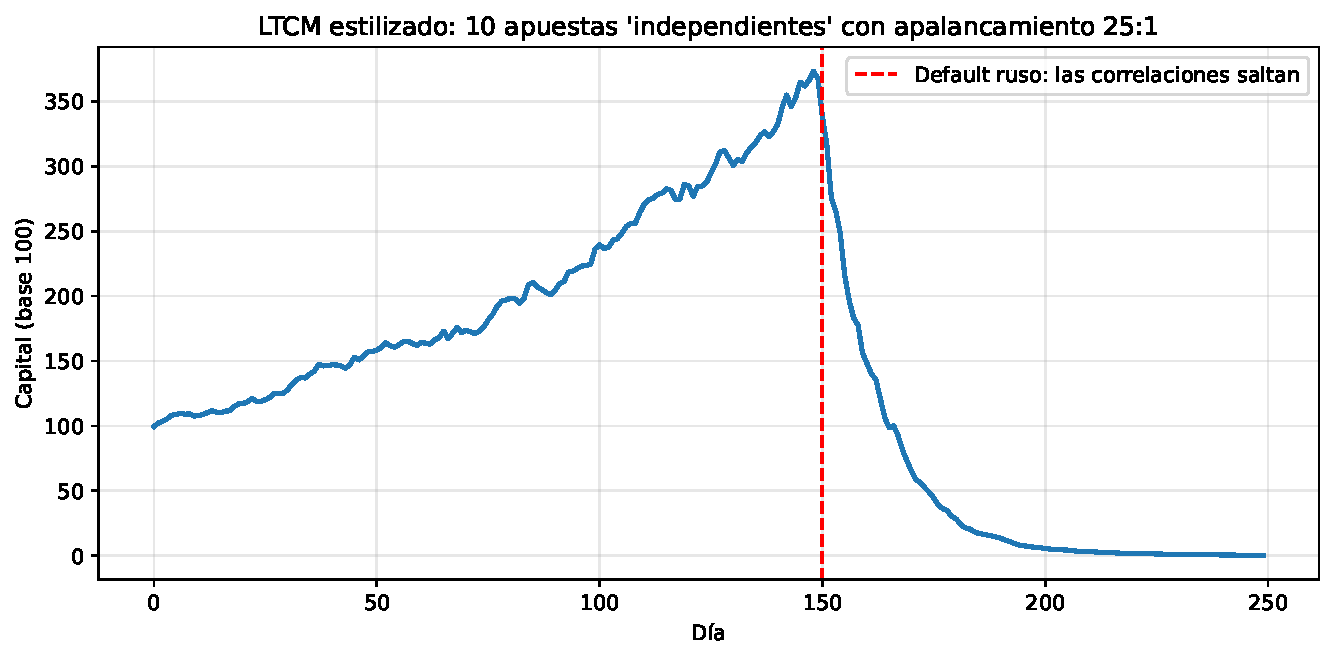
\includegraphics[keepaspectratio]{unidad3/cap12_riesgo_regulacion_files/figure-pdf/ltcm-simulacion-output-1.pdf}}

\begin{verbatim}
Capital final: 0 (arrancó en 100)
\end{verbatim}

Corré mentalmente el gráfico: meses de retornos suaves y consistentes
(la diversificación ``funciona'', el apalancamiento multiplica una
ganancia estable) y luego el precipicio, cuando las diez apuestas se
vuelven una sola y el 25:1 multiplica la pérdida. \textbf{Las lecciones
de LTCM}, que la industria recita desde entonces:

\begin{enumerate}
\def\labelenumi{\arabic{enumi}.}
\tightlist
\item
  \textbf{Las correlaciones históricas no son un contrato}: en las
  crisis convergen a 1, exactamente cuando la diversificación más se
  necesita.
\item
  \textbf{El apalancamiento convierte problemas de precio en problemas
  de supervivencia}: sin margen para esperar, tenés que vender en el
  peor momento.
\item
  \textbf{La liquidez es un riesgo en sí mismo}: LTCM tenía razón ``a
  largo plazo'' en muchas posiciones --- pero como dijo Keynes, el
  mercado puede permanecer irracional más tiempo del que vos podés
  permanecer solvente.
\item
  \textbf{El prestigio de los modelos (y de los Nobel) no es gestión de
  riesgo.}
\end{enumerate}

\begin{center}\rule{0.5\linewidth}{0.5pt}\end{center}

\chapter{Caso 2 --- 2008: la correlación
falsa}\label{caso-2-2008-la-correlaciuxf3n-falsa}

La crisis de 2008 es demasiado grande para un capítulo; acá nos
enfocamos en su \textbf{corazón cuantitativo}: cómo un supuesto de
correlación mal calibrado, industrializado a escala de billones de
dólares, hizo estallar el sistema.

\section{La maquinaria: securitización y
CDOs}\label{la-maquinaria-securitizaciuxf3n-y-cdos}

La cadena, simplificada: los bancos originaban \textbf{hipotecas}
(crecientemente \emph{subprime}, de baja calidad), las empaquetaban en
bonos (\textbf{MBS}), y luego empaquetaban esos bonos en \textbf{CDOs}
(\emph{Collateralized Debt Obligations}) divididos en \textbf{tramos}:
el tramo \emph{senior} cobra primero (y tenía calificación AAA), el
\emph{equity} absorbe las primeras pérdidas.

¿Cómo puede un paquete de hipotecas mediocres producir un tramo AAA? Por
la \textbf{diversificación}: si los defaults son suficientemente
\emph{independientes} entre sí, la probabilidad de que fallen
\emph{muchas a la vez} ---que es lo único que daña al tramo senior--- es
minúscula. Todo el edificio descansa en una pregunta: \textbf{¿cuán
correlacionados están los defaults de las hipotecas?}

\section{La fórmula: la cópula
gaussiana}\label{la-fuxf3rmula-la-cuxf3pula-gaussiana}

Para responderla, la industria adoptó masivamente la \textbf{cópula
gaussiana} de David Li (2000): un modelo elegante que describe la
dependencia entre defaults con un único parámetro de correlación
\(\rho\), calibrado con datos históricos\ldots{} de años en que la
vivienda en EEUU nunca había caído a escala nacional. La calibración
típica asumía correlaciones \textbf{bajas}: los defaults eran eventos
idiosincráticos (alguien pierde su empleo), no sistémicos.

El error fatal: cuando los precios de la vivienda caen a nivel nacional,
\textbf{todos los deudores subprime entran en problemas por la misma
causa al mismo tiempo}. La correlación real en el escenario relevante no
era 0.2: era cercana a 1.

\phantomsection\label{cdo-correlacion}
\begin{Shaded}
\begin{Highlighting}[]
\CommentTok{\# Un CDO de juguete: 100 hipotecas, tramo senior absorbe pérdidas \textgreater{} 25\%}
\NormalTok{n\_hipotecas, n\_escenarios }\OperatorTok{=} \DecValTok{100}\NormalTok{, }\DecValTok{50\_000}
\NormalTok{prob\_default, perdida\_por\_default }\OperatorTok{=} \FloatTok{0.08}\NormalTok{, }\FloatTok{0.5}   \CommentTok{\# 8\% de mora esperada, pierde 50\%}

\KeywordTok{def}\NormalTok{ perdida\_cartera(rho, rng):}
    \CommentTok{"""Modelo de un factor gaussiano: factor común (economía) + shock individual."""}
\NormalTok{    factor\_comun }\OperatorTok{=}\NormalTok{ rng.standard\_normal((n\_escenarios, }\DecValTok{1}\NormalTok{))}
\NormalTok{    idiosincratico }\OperatorTok{=}\NormalTok{ rng.standard\_normal((n\_escenarios, n\_hipotecas))}
\NormalTok{    salud }\OperatorTok{=}\NormalTok{ np.sqrt(rho) }\OperatorTok{*}\NormalTok{ factor\_comun }\OperatorTok{+}\NormalTok{ np.sqrt(}\DecValTok{1} \OperatorTok{{-}}\NormalTok{ rho) }\OperatorTok{*}\NormalTok{ idiosincratico}
\NormalTok{    umbral }\OperatorTok{=}\NormalTok{ stats.norm.ppf(prob\_default)}
\NormalTok{    defaults }\OperatorTok{=}\NormalTok{ salud }\OperatorTok{\textless{}}\NormalTok{ umbral}
    \ControlFlowTok{return}\NormalTok{ defaults.mean(axis}\OperatorTok{=}\DecValTok{1}\NormalTok{) }\OperatorTok{*}\NormalTok{ perdida\_por\_default}

\BuiltInTok{print}\NormalTok{(}\SpecialStringTok{f"}\SpecialCharTok{\{}\StringTok{\textquotesingle{}ρ\textquotesingle{}}\SpecialCharTok{:\textgreater{}5\}\{}\StringTok{\textquotesingle{}Pérdida media\textquotesingle{}}\SpecialCharTok{:\textgreater{}15\}\{}\StringTok{\textquotesingle{}P(pérdida \textgreater{} 25\%)\textquotesingle{}}\SpecialCharTok{:\textgreater{}20\}}\SpecialStringTok{   ¿El tramo senior (AAA) paga?"}\NormalTok{)}
\ControlFlowTok{for}\NormalTok{ rho }\KeywordTok{in}\NormalTok{ [}\FloatTok{0.05}\NormalTok{, }\FloatTok{0.20}\NormalTok{, }\FloatTok{0.60}\NormalTok{]:}
\NormalTok{    perdidas }\OperatorTok{=}\NormalTok{ perdida\_cartera(rho, np.random.default\_rng(}\DecValTok{1}\NormalTok{))}
\NormalTok{    p\_senior }\OperatorTok{=}\NormalTok{ (perdidas }\OperatorTok{\textgreater{}} \FloatTok{0.25}\NormalTok{).mean()}
    \BuiltInTok{print}\NormalTok{(}\SpecialStringTok{f"}\SpecialCharTok{\{}\NormalTok{rho}\SpecialCharTok{:\textgreater{}5.2f\}\{}\NormalTok{perdidas}\SpecialCharTok{.}\NormalTok{mean()}\SpecialCharTok{:\textgreater{}14.1\%\}\{}\NormalTok{p\_senior}\SpecialCharTok{:\textgreater{}19.2\%\}}\SpecialStringTok{   "}
          \SpecialStringTok{f"}\SpecialCharTok{\{}\StringTok{\textquotesingle{}casi siempre\textquotesingle{}} \ControlFlowTok{if}\NormalTok{ p\_senior }\OperatorTok{\textless{}} \FloatTok{0.005} \ControlFlowTok{else} \StringTok{\textquotesingle{}NO: riesgo real\textquotesingle{}}\SpecialCharTok{\}}\SpecialStringTok{"}\NormalTok{)}
\end{Highlighting}
\end{Shaded}

\begin{verbatim}
    ρ  Pérdida media    P(pérdida > 25%)   ¿El tramo senior (AAA) paga?
 0.05          4.0%              0.00%   casi siempre
 0.20          4.0%              0.09%   casi siempre
 0.60          4.0%              3.39%   NO: riesgo real
\end{verbatim}

Mirá la tabla: la \textbf{pérdida promedio es la misma} en las tres
filas (la correlación no cambia cuántas hipotecas caen \emph{en
promedio}), pero la probabilidad de que la pérdida atraviese el tramo
senior \textbf{se multiplica por órdenes de magnitud} al subir \(\rho\).
Con \(\rho\) bajo, las pérdidas siempre rondan el promedio y el AAA es
intocable; con \(\rho\) alto, la distribución se vuelve bimodal --- o no
pasa casi nada, \textbf{o caen todas juntas}. El mismo instrumento, la
misma mora esperada\ldots{} y calificaciones que pasaron de
``prácticamente libre de riesgo'' a basura en cuestión de meses de
2007-2008.

El resto de la historia se sigue de ahí: los tramos AAA estaban en todos
lados (bancos, fondos, aseguradoras como AIG que los aseguraban vía
CDS), nadie sabía quién tenía cuánto, el interbancario se congeló,
Lehman cayó, y el mundo descubrió la diferencia entre \emph{riesgo} (lo
que el modelo mide) e \emph{incertidumbre} (lo que el modelo ni siquiera
contempla).

\textbf{Las lecciones de 2008} para el modelador:

\begin{enumerate}
\def\labelenumi{\arabic{enumi}.}
\tightlist
\item
  \textbf{Un parámetro calibrado en tiempos de calma no describe la
  crisis}: la correlación es \emph{condicional al régimen}, y el régimen
  que importa es el peor.
\item
  \textbf{La elegancia matemática no valida los supuestos}: la cópula
  gaussiana era tratable y estándar; su supuesto central era falso.
\item
  \textbf{El riesgo de modelo se industrializa}: un modelo mediocre
  usado por una mesa es un problema local; usado por toda la industria
  para calificar billones, es sistémico.
\item
  \textbf{Las colas y la dependencia extrema importan más que el
  centro}: dos distribuciones con la misma media y varianza pueden tener
  riesgos de cola radicalmente distintos --- el puente perfecto hacia el
  próximo capítulo.
\end{enumerate}

\begin{center}\rule{0.5\linewidth}{0.5pt}\end{center}

\chapter{Errores comunes}\label{errores-comunes-10}

\begin{tcolorbox}[enhanced jigsaw, bottomrule=.15mm, colback=white, opacitybacktitle=0.6, arc=.35mm, toprule=.15mm, opacityback=0, breakable, titlerule=0mm, left=2mm, coltitle=black, colbacktitle=quarto-callout-warning-color!10!white, colframe=quarto-callout-warning-color-frame, leftrule=.75mm, toptitle=1mm, bottomtitle=1mm, title=\textcolor{quarto-callout-warning-color}{\faExclamationTriangle}\hspace{0.5em}{Trampas conceptuales de este capítulo}, rightrule=.15mm]

\begin{itemize}
\tightlist
\item
  \textbf{Tratar la correlación como constante}: es la trampa que une
  LTCM y 2008. Estimá correlaciones condicionales a regímenes de estrés,
  no promedios históricos.
\item
  \textbf{Confundir solvencia con liquidez}: podés tener razón en la
  valuación y quebrar igual si el fondeo desaparece antes de que el
  precio converja.
\item
  \textbf{Leer los stress tests como pronósticos}: un escenario no es
  una predicción; es una linterna apuntada a una vulnerabilidad.
\item
  \textbf{Creer que la regulación elimina el riesgo}: lo redistribuye y
  lo acota. Cada marco regulatorio genera, además, sus propios
  incentivos y puntos ciegos (el arbitraje regulatorio de los RWA fue
  parte del problema en 2008).
\end{itemize}

\end{tcolorbox}

\begin{center}\rule{0.5\linewidth}{0.5pt}\end{center}

\chapter{Ejercicios Propuestos}\label{ejercicios-propuestos-11}

\begin{tcolorbox}[enhanced jigsaw, bottomrule=.15mm, colback=white, opacitybacktitle=0.6, arc=.35mm, toprule=.15mm, opacityback=0, breakable, titlerule=0mm, left=2mm, coltitle=black, colbacktitle=quarto-callout-important-color!10!white, colframe=quarto-callout-important-color-frame, leftrule=.75mm, toptitle=1mm, bottomtitle=1mm, title=\textcolor{quarto-callout-important-color}{\faExclamation}\hspace{0.5em}{Ejercicios}, rightrule=.15mm]

\begin{enumerate}
\def\labelenumi{\arabic{enumi}.}
\tightlist
\item
  \textbf{Escenario propio}: definí un escenario hipotético para la
  economía argentina (salto del tipo de cambio, caída de bonos, suba de
  tasas) y aplicáselo a la cartera del inicio del capítulo. Justificá
  los shocks elegidos.
\item
  \textbf{Sensibilidad del RWA}: recalculá el ratio CET1 del banco de
  ejemplo si las hipotecas pasan a ponderar 50\% y los préstamos PyME
  100\%. ¿Cuánto capital adicional necesita para mantener 10.5\%?
\item
  \textbf{LTCM paramétrico}: en la simulación de LTCM, barré el
  apalancamiento de 5:1 a 30:1 y graficá el capital final en cada caso.
  ¿A partir de qué nivel el fondo no sobrevive a la crisis?
\item
  \textbf{La bimodalidad del CDO}: graficá el histograma de pérdidas de
  la cartera hipotecaria para \(\rho = 0.05\) y \(\rho = 0.6\). Describí
  la diferencia de forma --- ahí está toda la crisis de 2008.
\item
  \textbf{Correlación condicional}: con datos reales de dos índices
  bursátiles, estimá la correlación usando solo los días en que ambos
  caen más de 1\%. Comparala con la correlación incondicional.
\end{enumerate}

\end{tcolorbox}

Podés resolver estos ejercicios acá mismo: la celda ejecuta Python
\textbf{en tu navegador}, sin instalar nada (la primera ejecución tarda
unos segundos mientras carga el entorno; los paquetes que importes se
instalan solos).

\begin{Shaded}
\begin{Highlighting}[]
\NormalTok{\#| label: practica{-}navegador}
\NormalTok{import numpy as np}

\NormalTok{rng = np.random.default\_rng(42)}

\NormalTok{\# Tu solución acá...}
\end{Highlighting}
\end{Shaded}

\begin{center}\rule{0.5\linewidth}{0.5pt}\end{center}

\chapter{Referencias}\label{referencias-11}

\phantomsection\label{refs}

\chapter{Capítulo 13: Simulación de Monte
Carlo}\label{capuxedtulo-13-simulaciuxf3n-de-monte-carlo}

Movimiento Browniano Geométrico y generación de escenarios

Cuando un problema no tiene fórmula cerrada, la simulación de Monte
Carlo lo resuelve por fuerza bruta inteligente: generar miles de futuros
posibles y estudiar su distribución. Presentamos el Movimiento Browniano
Geométrico como modelo canónico del precio de un activo, simulamos
trayectorias de forma vectorizada, calculamos VaR y Expected Shortfall
por simulación, estudiamos la convergencia del método y lo aceleramos
con variables antitéticas. Cerramos valuando una opción, el puente hacia
el Módulo 4.

\hfill\break

\chapter{Introducción}\label{introducciuxf3n-10}

Hay preguntas financieras que no tienen fórmula: \emph{¿cuál es la
distribución del valor de mi cartera en 5 años si rebalanceo cada mes?
¿cuánto vale una opción cuyo pago depende de la trayectoria del precio y
no solo del valor final?} Para ese tipo de problemas existe el método de
\textbf{Monte Carlo}, llamado así por el casino: en lugar de resolver el
problema analíticamente, \textbf{tiramos los dados miles de veces}
---simulamos miles de futuros posibles--- y estudiamos la distribución
de resultados.

La receta general tiene tres pasos:

\begin{enumerate}
\def\labelenumi{\arabic{enumi}.}
\tightlist
\item
  \textbf{Modelar} la dinámica de la variable incierta (para nosotros:
  el precio de un activo).
\item
  \textbf{Simular} muchas trayectorias independientes de ese modelo.
\item
  \textbf{Agregar}: estimar lo que nos interese (media, percentiles,
  probabilidad de un evento) sobre las trayectorias.
\end{enumerate}

El paso 1 exige elegir un modelo del precio. Empezamos por el más
importante de todos: el \textbf{Movimiento Browniano Geométrico}.

\phantomsection\label{setup}
\begin{Shaded}
\begin{Highlighting}[]
\ImportTok{import}\NormalTok{ numpy }\ImportTok{as}\NormalTok{ np}
\ImportTok{import}\NormalTok{ matplotlib.pyplot }\ImportTok{as}\NormalTok{ plt}
\ImportTok{from}\NormalTok{ scipy }\ImportTok{import}\NormalTok{ stats}

\NormalTok{rng }\OperatorTok{=}\NormalTok{ np.random.default\_rng(}\DecValTok{42}\NormalTok{)}
\end{Highlighting}
\end{Shaded}

\begin{center}\rule{0.5\linewidth}{0.5pt}\end{center}

\chapter{El Movimiento Browniano Geométrico
(GBM)}\label{el-movimiento-browniano-geomuxe9trico-gbm}

\section{La idea}\label{la-idea}

¿Cómo modelar el precio de una acción? Dos observaciones empíricas nos
guían:

\begin{itemize}
\tightlist
\item
  Los precios tienen una \textbf{tendencia} de largo plazo (el mercado
  sube ``en promedio'').
\item
  Alrededor de esa tendencia hay \textbf{ruido} permanente e
  impredecible.
\end{itemize}

El GBM formaliza exactamente eso. En su forma de ecuación diferencial
estocástica:

\[\frac{dS}{S} = \mu \, dt + \sigma \, dW\]

Leela por partes: el retorno instantáneo del activo (\(dS/S\)) tiene un
componente determinístico \(\mu\,dt\) (el \textbf{drift}, la tendencia)
y un componente aleatorio \(\sigma\,dW\) (la \textbf{difusión}: ruido
gaussiano escalado por la volatilidad). Es literalmente ``tendencia +
ruido''.

Para simular necesitamos la versión discreta. Integrando la ecuación
(los detalles requieren cálculo estocástico, pero el resultado es lo que
importa):

\[S_{t+\Delta t} = S_t \cdot \exp\!\Big[\big(\mu - \tfrac{\sigma^2}{2}\big)\Delta t + \sigma \sqrt{\Delta t} \, Z\Big], \qquad Z \sim N(0,1)\]

\begin{tcolorbox}[enhanced jigsaw, bottomrule=.15mm, colback=white, opacitybacktitle=0.6, arc=.35mm, toprule=.15mm, opacityback=0, breakable, titlerule=0mm, left=2mm, coltitle=black, colbacktitle=quarto-callout-note-color!10!white, colframe=quarto-callout-note-color-frame, leftrule=.75mm, toptitle=1mm, bottomtitle=1mm, title=\textcolor{quarto-callout-note-color}{\faInfo}\hspace{0.5em}{¿De dónde sale el −σ²/2?}, rightrule=.15mm]

Ese término sorprende la primera vez. La intuición: la exponencial es
convexa, así que el ruido simétrico en el exponente produce resultados
\emph{asimétricos} en el precio (una suba del 10\% seguida de una baja
del 10\% no te devuelve al punto de partida: \(1.1 \times 0.9 = 0.99\)).
El término \(-\sigma^2/2\) corrige exactamente ese efecto para que el
retorno \emph{esperado} del precio sea \(\mu\). Sin la corrección, la
simulación tendría un sesgo alcista espurio.

\end{tcolorbox}

Dos propiedades del GBM que conviene tener presentes:

\begin{itemize}
\tightlist
\item
  El precio \textbf{nunca se hace negativo} (es una exponencial) ---
  realista para acciones.
\item
  Los retornos logarítmicos son normales, así que el precio final es
  \textbf{lognormal}: asimétrico, con una cola larga hacia arriba.
\end{itemize}

\section{Simulación vectorizada}\label{simulaciuxf3n-vectorizada}

Simulamos \textbf{todas las trayectorias a la vez} con una matriz de
shocks: filas = pasos de tiempo, columnas = simulaciones. El único bucle
recorre el tiempo (cada precio depende del anterior); las 10.000
simulaciones avanzan en paralelo gracias a la vectorización del Capítulo
5.

\phantomsection\label{gbm}
\begin{Shaded}
\begin{Highlighting}[]
\CommentTok{\# Parámetros del activo y de la simulación}
\NormalTok{S0 }\OperatorTok{=} \DecValTok{100}          \CommentTok{\# precio inicial}
\NormalTok{mu }\OperatorTok{=} \FloatTok{0.10}         \CommentTok{\# drift anual (10\%)}
\NormalTok{sigma }\OperatorTok{=} \FloatTok{0.25}      \CommentTok{\# volatilidad anual (25\%)}
\NormalTok{T }\OperatorTok{=} \FloatTok{1.0}           \CommentTok{\# horizonte: 1 año}
\NormalTok{n\_pasos }\OperatorTok{=} \DecValTok{252}     \CommentTok{\# pasos diarios}
\NormalTok{n\_sims }\OperatorTok{=} \DecValTok{10\_000}   \CommentTok{\# trayectorias}

\NormalTok{dt }\OperatorTok{=}\NormalTok{ T }\OperatorTok{/}\NormalTok{ n\_pasos}

\CommentTok{\# Matriz de shocks: un N(0,1) por paso y por simulación}
\NormalTok{Z }\OperatorTok{=}\NormalTok{ rng.standard\_normal((n\_pasos, n\_sims))}

\CommentTok{\# Simulación: el bucle recorre el tiempo; las columnas avanzan en paralelo}
\NormalTok{S }\OperatorTok{=}\NormalTok{ np.empty((n\_pasos }\OperatorTok{+} \DecValTok{1}\NormalTok{, n\_sims))}
\NormalTok{S[}\DecValTok{0}\NormalTok{] }\OperatorTok{=}\NormalTok{ S0}
\ControlFlowTok{for}\NormalTok{ t }\KeywordTok{in} \BuiltInTok{range}\NormalTok{(}\DecValTok{1}\NormalTok{, n\_pasos }\OperatorTok{+} \DecValTok{1}\NormalTok{):}
\NormalTok{    S[t] }\OperatorTok{=}\NormalTok{ S[t}\OperatorTok{{-}}\DecValTok{1}\NormalTok{] }\OperatorTok{*}\NormalTok{ np.exp((mu }\OperatorTok{{-}} \FloatTok{0.5} \OperatorTok{*}\NormalTok{ sigma}\OperatorTok{**}\DecValTok{2}\NormalTok{) }\OperatorTok{*}\NormalTok{ dt }\OperatorTok{+}\NormalTok{ sigma }\OperatorTok{*}\NormalTok{ np.sqrt(dt) }\OperatorTok{*}\NormalTok{ Z[t}\OperatorTok{{-}}\DecValTok{1}\NormalTok{])}

\BuiltInTok{print}\NormalTok{(}\SpecialStringTok{f"Precio inicial:       $}\SpecialCharTok{\{}\NormalTok{S0}\SpecialCharTok{:.2f\}}\SpecialStringTok{"}\NormalTok{)}
\BuiltInTok{print}\NormalTok{(}\SpecialStringTok{f"Precio medio final:   $}\SpecialCharTok{\{}\NormalTok{S[}\OperatorTok{{-}}\DecValTok{1}\NormalTok{]}\SpecialCharTok{.}\NormalTok{mean()}\SpecialCharTok{:.2f\}}\SpecialStringTok{   (teórico: $}\SpecialCharTok{\{}\NormalTok{S0 }\OperatorTok{*}\NormalTok{ np}\SpecialCharTok{.}\NormalTok{exp(mu }\OperatorTok{*}\NormalTok{ T)}\SpecialCharTok{:.2f\}}\SpecialStringTok{)"}\NormalTok{)}
\BuiltInTok{print}\NormalTok{(}\SpecialStringTok{f"Precio mediano final: $}\SpecialCharTok{\{}\NormalTok{np}\SpecialCharTok{.}\NormalTok{median(S[}\OperatorTok{{-}}\DecValTok{1}\NormalTok{])}\SpecialCharTok{:.2f\}}\SpecialStringTok{"}\NormalTok{)}
\BuiltInTok{print}\NormalTok{(}\SpecialStringTok{f"Rango simulado:       $}\SpecialCharTok{\{}\NormalTok{S[}\OperatorTok{{-}}\DecValTok{1}\NormalTok{]}\SpecialCharTok{.}\BuiltInTok{min}\NormalTok{()}\SpecialCharTok{:.2f\}}\SpecialStringTok{ — $}\SpecialCharTok{\{}\NormalTok{S[}\OperatorTok{{-}}\DecValTok{1}\NormalTok{]}\SpecialCharTok{.}\BuiltInTok{max}\NormalTok{()}\SpecialCharTok{:.2f\}}\SpecialStringTok{"}\NormalTok{)}
\end{Highlighting}
\end{Shaded}

\begin{verbatim}
Precio inicial:       $100.00
Precio medio final:   $110.78   (teórico: $110.52)
Precio mediano final: $107.23
Rango simulado:       $43.61 — $265.43
\end{verbatim}

Verificación de cordura: la media simulada coincide con la teórica
\(E[S_T] = S_0 e^{\mu T}\). Notá también que la \textbf{mediana está por
debajo de la media}: es la asimetría lognormal en acción (unas pocas
trayectorias excelentes tiran el promedio hacia arriba).

\begin{Shaded}
\begin{Highlighting}[]
\NormalTok{fig, axes }\OperatorTok{=}\NormalTok{ plt.subplots(}\DecValTok{1}\NormalTok{, }\DecValTok{2}\NormalTok{, figsize}\OperatorTok{=}\NormalTok{(}\DecValTok{12}\NormalTok{, }\FloatTok{4.5}\NormalTok{))}

\CommentTok{\# Panel 1: una muestra de trayectorias}
\NormalTok{ax }\OperatorTok{=}\NormalTok{ axes[}\DecValTok{0}\NormalTok{]}
\NormalTok{tiempo }\OperatorTok{=}\NormalTok{ np.arange(n\_pasos }\OperatorTok{+} \DecValTok{1}\NormalTok{) }\OperatorTok{/} \DecValTok{252}
\NormalTok{ax.plot(tiempo, S[:, :}\DecValTok{100}\NormalTok{], alpha}\OperatorTok{=}\FloatTok{0.25}\NormalTok{, linewidth}\OperatorTok{=}\FloatTok{0.6}\NormalTok{)}
\NormalTok{ax.plot(tiempo, S0 }\OperatorTok{*}\NormalTok{ np.exp(mu }\OperatorTok{*}\NormalTok{ tiempo), }\StringTok{"k{-}{-}"}\NormalTok{, linewidth}\OperatorTok{=}\DecValTok{2}\NormalTok{, label}\OperatorTok{=}\StringTok{"Tendencia $S\_0 e\^{}\{}\CharTok{\textbackslash{}\textbackslash{}}\StringTok{mu t\}$"}\NormalTok{)}
\NormalTok{ax.set\_title(}\SpecialStringTok{f"100 trayectorias (de }\SpecialCharTok{\{}\NormalTok{n\_sims}\SpecialCharTok{:,\}}\SpecialStringTok{)"}\NormalTok{)}
\NormalTok{ax.set\_xlabel(}\StringTok{"Años"}\NormalTok{)}
\NormalTok{ax.set\_ylabel(}\StringTok{"Precio ($)"}\NormalTok{)}
\NormalTok{ax.legend()}
\NormalTok{ax.grid(}\VariableTok{True}\NormalTok{, alpha}\OperatorTok{=}\FloatTok{0.3}\NormalTok{)}

\CommentTok{\# Panel 2: distribución de precios finales}
\NormalTok{ax }\OperatorTok{=}\NormalTok{ axes[}\DecValTok{1}\NormalTok{]}
\NormalTok{ax.hist(S[}\OperatorTok{{-}}\DecValTok{1}\NormalTok{], bins}\OperatorTok{=}\DecValTok{80}\NormalTok{, density}\OperatorTok{=}\VariableTok{True}\NormalTok{, alpha}\OperatorTok{=}\FloatTok{0.7}\NormalTok{, color}\OperatorTok{=}\StringTok{"steelblue"}\NormalTok{, edgecolor}\OperatorTok{=}\StringTok{"white"}\NormalTok{)}
\NormalTok{ax.axvline(S[}\OperatorTok{{-}}\DecValTok{1}\NormalTok{].mean(), color}\OperatorTok{=}\StringTok{"green"}\NormalTok{, linestyle}\OperatorTok{=}\StringTok{"{-}{-}"}\NormalTok{,}
\NormalTok{           label}\OperatorTok{=}\SpecialStringTok{f"Media: $}\SpecialCharTok{\{}\NormalTok{S[}\OperatorTok{{-}}\DecValTok{1}\NormalTok{]}\SpecialCharTok{.}\NormalTok{mean()}\SpecialCharTok{:.0f\}}\SpecialStringTok{"}\NormalTok{)}
\NormalTok{ax.axvline(np.median(S[}\OperatorTok{{-}}\DecValTok{1}\NormalTok{]), color}\OperatorTok{=}\StringTok{"red"}\NormalTok{, linestyle}\OperatorTok{=}\StringTok{":"}\NormalTok{,}
\NormalTok{           label}\OperatorTok{=}\SpecialStringTok{f"Mediana: $}\SpecialCharTok{\{}\NormalTok{np}\SpecialCharTok{.}\NormalTok{median(S[}\OperatorTok{{-}}\DecValTok{1}\NormalTok{])}\SpecialCharTok{:.0f\}}\SpecialStringTok{"}\NormalTok{)}
\NormalTok{ax.set\_title(}\StringTok{"Distribución de $S\_T$ (lognormal)"}\NormalTok{)}
\NormalTok{ax.set\_xlabel(}\StringTok{"Precio final ($)"}\NormalTok{)}
\NormalTok{ax.legend()}
\NormalTok{ax.grid(}\VariableTok{True}\NormalTok{, alpha}\OperatorTok{=}\FloatTok{0.3}\NormalTok{)}

\NormalTok{plt.tight\_layout()}
\NormalTok{plt.show()}
\end{Highlighting}
\end{Shaded}

\pandocbounded{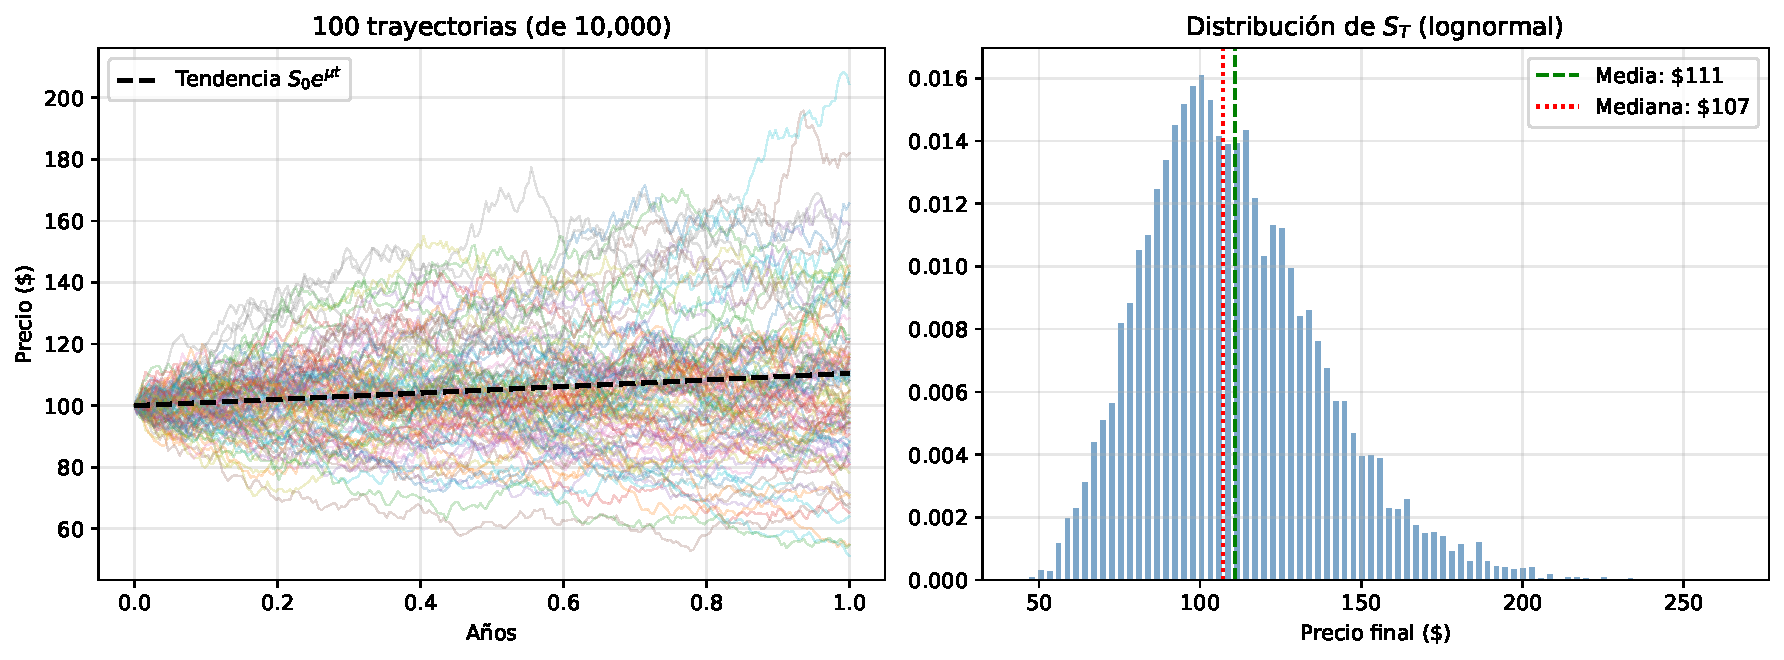
\includegraphics[keepaspectratio]{unidad3/cap13_monte_carlo_files/figure-pdf/plot-caminos-output-1.pdf}}

El panel izquierdo es el ``abanico de futuros'': todas las trayectorias
arrancan del mismo punto y se dispersan con el tiempo. El derecho resume
dónde terminan: la forma asimétrica con cola derecha larga es la
distribución lognormal.

\begin{center}\rule{0.5\linewidth}{0.5pt}\end{center}

\chapter{VaR y Expected Shortfall por Monte
Carlo}\label{var-y-expected-shortfall-por-monte-carlo}

En el Capítulo 11 calculamos VaR y ES con dos métodos: paramétrico
(asume normal) e histórico (usa el pasado). Monte Carlo es el
\textbf{tercer método}, y el más flexible: la distribución de pérdidas
sale de las trayectorias simuladas, con el modelo que queramos. Hoy el
modelo es GBM; en el próximo capítulo será uno con saltos --- y el
código de abajo no cambia.

\phantomsection\label{var-montecarlo}
\begin{Shaded}
\begin{Highlighting}[]
\NormalTok{valor\_portafolio }\OperatorTok{=} \DecValTok{10\_000\_000}
\NormalTok{retornos\_sim }\OperatorTok{=}\NormalTok{ S[}\OperatorTok{{-}}\DecValTok{1}\NormalTok{] }\OperatorTok{/}\NormalTok{ S0 }\OperatorTok{{-}} \DecValTok{1}     \CommentTok{\# retorno de cada trayectoria a 1 año}

\NormalTok{var\_95 }\OperatorTok{=} \OperatorTok{{-}}\NormalTok{np.percentile(retornos\_sim, }\DecValTok{5}\NormalTok{) }\OperatorTok{*}\NormalTok{ valor\_portafolio}
\NormalTok{umbral }\OperatorTok{=}\NormalTok{ np.percentile(retornos\_sim, }\DecValTok{5}\NormalTok{)}
\NormalTok{es\_95 }\OperatorTok{=} \OperatorTok{{-}}\NormalTok{retornos\_sim[retornos\_sim }\OperatorTok{\textless{}=}\NormalTok{ umbral].mean() }\OperatorTok{*}\NormalTok{ valor\_portafolio}

\BuiltInTok{print}\NormalTok{(}\SpecialStringTok{f"Sobre un portafolio de $}\SpecialCharTok{\{}\NormalTok{valor\_portafolio}\OperatorTok{/}\FloatTok{1e6}\SpecialCharTok{:.0f\}}\SpecialStringTok{M, horizonte 1 año:"}\NormalTok{)}
\BuiltInTok{print}\NormalTok{(}\SpecialStringTok{f"  VaR 95\% (Monte Carlo): $}\SpecialCharTok{\{}\NormalTok{var\_95}\SpecialCharTok{:\textgreater{}12,.0f\}}\SpecialStringTok{"}\NormalTok{)}
\BuiltInTok{print}\NormalTok{(}\SpecialStringTok{f"  ES  95\% (Monte Carlo): $}\SpecialCharTok{\{}\NormalTok{es\_95}\SpecialCharTok{:\textgreater{}12,.0f\}}\SpecialStringTok{"}\NormalTok{)}
\end{Highlighting}
\end{Shaded}

\begin{verbatim}
Sobre un portafolio de $10M, horizonte 1 año:
  VaR 95% (Monte Carlo): $   2,921,024
  ES  95% (Monte Carlo): $   3,594,308
\end{verbatim}

\begin{center}\rule{0.5\linewidth}{0.5pt}\end{center}

\chapter{¿Cuántas simulaciones son suficientes?
Convergencia}\label{cuuxe1ntas-simulaciones-son-suficientes-convergencia}

Monte Carlo da una \textbf{estimación}, no un valor exacto, y su error
decrece con la raíz del número de simulaciones:
\(\text{error} \propto 1/\sqrt{N}\). Esa raíz es una mala noticia
práctica: para ganar \textbf{un dígito} de precisión hay que multiplicar
las simulaciones \textbf{por 100}.

\begin{Shaded}
\begin{Highlighting}[]
\NormalTok{ns }\OperatorTok{=}\NormalTok{ np.unique(np.logspace(}\DecValTok{2}\NormalTok{, }\DecValTok{4}\NormalTok{, }\DecValTok{25}\NormalTok{).astype(}\BuiltInTok{int}\NormalTok{))}
\NormalTok{medias }\OperatorTok{=}\NormalTok{ [S[}\OperatorTok{{-}}\DecValTok{1}\NormalTok{, :n].mean() }\ControlFlowTok{for}\NormalTok{ n }\KeywordTok{in}\NormalTok{ ns]}
\NormalTok{teorico }\OperatorTok{=}\NormalTok{ S0 }\OperatorTok{*}\NormalTok{ np.exp(mu }\OperatorTok{*}\NormalTok{ T)}

\CommentTok{\# Banda de error teórica: ±2 desvíos del estimador de la media}
\NormalTok{sd\_ST }\OperatorTok{=}\NormalTok{ S[}\OperatorTok{{-}}\DecValTok{1}\NormalTok{].std()}
\NormalTok{banda }\OperatorTok{=} \DecValTok{2} \OperatorTok{*}\NormalTok{ sd\_ST }\OperatorTok{/}\NormalTok{ np.sqrt(ns)}

\NormalTok{fig, ax }\OperatorTok{=}\NormalTok{ plt.subplots(figsize}\OperatorTok{=}\NormalTok{(}\DecValTok{9}\NormalTok{, }\FloatTok{4.5}\NormalTok{))}
\NormalTok{ax.plot(ns, medias, }\StringTok{"o{-}"}\NormalTok{, color}\OperatorTok{=}\StringTok{"steelblue"}\NormalTok{, markersize}\OperatorTok{=}\DecValTok{4}\NormalTok{, label}\OperatorTok{=}\StringTok{"Media estimada"}\NormalTok{)}
\NormalTok{ax.axhline(teorico, color}\OperatorTok{=}\StringTok{"red"}\NormalTok{, linestyle}\OperatorTok{=}\StringTok{"{-}{-}"}\NormalTok{, label}\OperatorTok{=}\SpecialStringTok{f"Valor teórico ($}\SpecialCharTok{\{}\NormalTok{teorico}\SpecialCharTok{:.2f\}}\SpecialStringTok{)"}\NormalTok{)}
\NormalTok{ax.fill\_between(ns, teorico }\OperatorTok{{-}}\NormalTok{ banda, teorico }\OperatorTok{+}\NormalTok{ banda, alpha}\OperatorTok{=}\FloatTok{0.15}\NormalTok{, color}\OperatorTok{=}\StringTok{"red"}\NormalTok{,}
\NormalTok{                label}\OperatorTok{=}\StringTok{"Banda ±2 errores estándar"}\NormalTok{)}
\NormalTok{ax.set\_xscale(}\StringTok{"log"}\NormalTok{)}
\NormalTok{ax.set\_xlabel(}\StringTok{"Número de simulaciones (escala log)"}\NormalTok{)}
\NormalTok{ax.set\_ylabel(}\StringTok{"Precio medio final ($)"}\NormalTok{)}
\NormalTok{ax.set\_title(}\StringTok{"Convergencia de Monte Carlo: el error cae como 1/√N"}\NormalTok{)}
\NormalTok{ax.legend()}
\NormalTok{ax.grid(}\VariableTok{True}\NormalTok{, alpha}\OperatorTok{=}\FloatTok{0.3}\NormalTok{)}
\NormalTok{plt.tight\_layout()}
\NormalTok{plt.show()}
\end{Highlighting}
\end{Shaded}

\pandocbounded{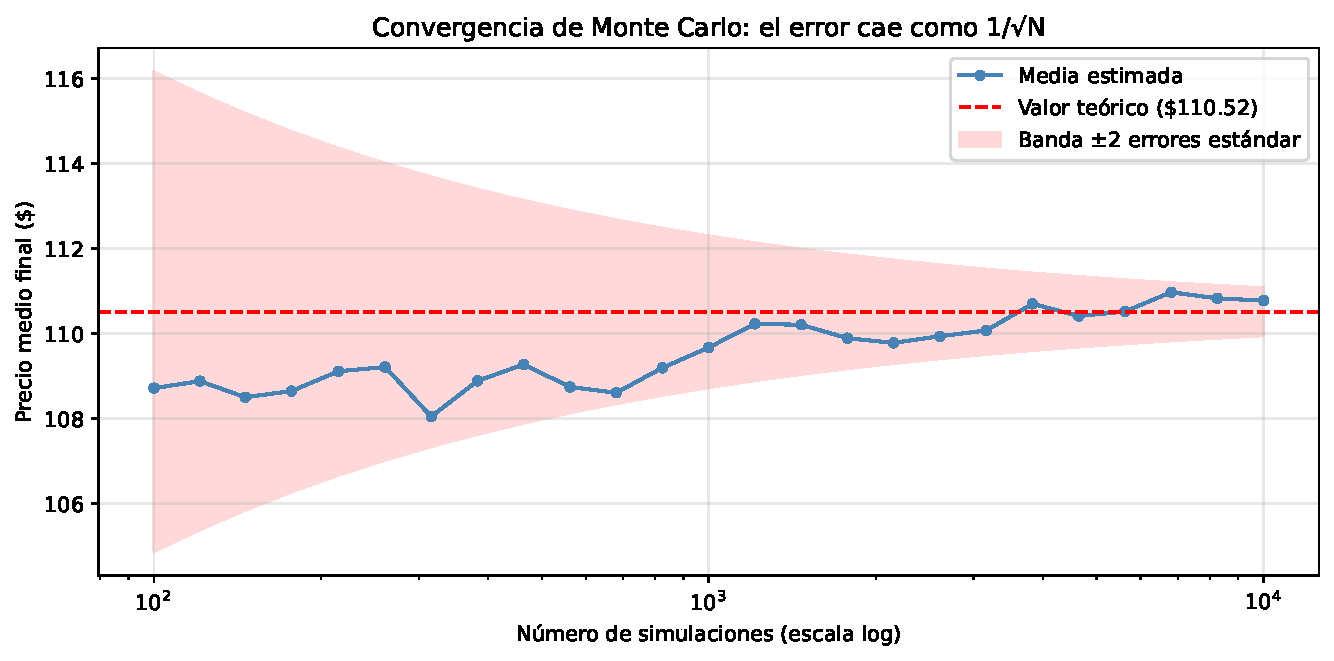
\includegraphics[keepaspectratio]{unidad3/cap13_monte_carlo_files/figure-pdf/convergencia-output-1.pdf}}

La estimación ``baila'' dentro de la banda teórica y se aquieta a medida
que \(N\) crece. Regla práctica: reportá siempre el \textbf{error
estándar} de tu estimación Monte Carlo (\(s/\sqrt{N}\)), no solo el
número.

\section{Reducción de varianza: variables
antitéticas}\label{reducciuxf3n-de-varianza-variables-antituxe9ticas}

¿Se puede lograr más precisión sin más simulaciones? Sí --- hay toda una
familia de técnicas de \textbf{reducción de varianza}. La más simple y
elegante: las \textbf{variables antitéticas}. La idea: por cada shock
\(Z\) que uses, usá también \(-Z\). Cada trayectoria ``optimista'' queda
emparejada con su gemela ``pesimista'', los errores de ambas se
compensan, y el promedio del par es mucho más estable que dos
trayectorias independientes.

\phantomsection\label{antiteticas}
\begin{Shaded}
\begin{Highlighting}[]
\KeywordTok{def}\NormalTok{ precio\_final\_gbm(Z):}
    \CommentTok{"""Precio final S\_T dado un vector de shocks acumulados por trayectoria."""}
\NormalTok{    log\_ST }\OperatorTok{=}\NormalTok{ (np.log(S0) }\OperatorTok{+}\NormalTok{ (mu }\OperatorTok{{-}} \FloatTok{0.5} \OperatorTok{*}\NormalTok{ sigma}\OperatorTok{**}\DecValTok{2}\NormalTok{) }\OperatorTok{*}\NormalTok{ T}
              \OperatorTok{+}\NormalTok{ sigma }\OperatorTok{*}\NormalTok{ np.sqrt(dt) }\OperatorTok{*}\NormalTok{ Z.}\BuiltInTok{sum}\NormalTok{(axis}\OperatorTok{=}\DecValTok{0}\NormalTok{))}
    \ControlFlowTok{return}\NormalTok{ np.exp(log\_ST)}

\NormalTok{n\_pares }\OperatorTok{=}\NormalTok{ n\_sims }\OperatorTok{//} \DecValTok{2}
\NormalTok{Z\_half }\OperatorTok{=}\NormalTok{ rng.standard\_normal((n\_pasos, n\_pares))}

\CommentTok{\# Método estándar: n\_sims trayectorias independientes}
\NormalTok{ST\_std }\OperatorTok{=}\NormalTok{ precio\_final\_gbm(rng.standard\_normal((n\_pasos, n\_sims)))}

\CommentTok{\# Método antitético: n\_pares trayectorias + sus espejos (mismo costo total)}
\NormalTok{ST\_pos }\OperatorTok{=}\NormalTok{ precio\_final\_gbm(Z\_half)}
\NormalTok{ST\_neg }\OperatorTok{=}\NormalTok{ precio\_final\_gbm(}\OperatorTok{{-}}\NormalTok{Z\_half)}
\NormalTok{ST\_anti }\OperatorTok{=} \FloatTok{0.5} \OperatorTok{*}\NormalTok{ (ST\_pos }\OperatorTok{+}\NormalTok{ ST\_neg)      }\CommentTok{\# promedio por par}

\BuiltInTok{print}\NormalTok{(}\SpecialStringTok{f"}\SpecialCharTok{\{}\StringTok{\textquotesingle{}\textquotesingle{}}\SpecialCharTok{:24\}\{}\StringTok{\textquotesingle{}Estimación\textquotesingle{}}\SpecialCharTok{:\textgreater{}12\}\{}\StringTok{\textquotesingle{}Error estándar\textquotesingle{}}\SpecialCharTok{:\textgreater{}16\}}\SpecialStringTok{"}\NormalTok{)}
\BuiltInTok{print}\NormalTok{(}\SpecialStringTok{f"}\SpecialCharTok{\{}\StringTok{\textquotesingle{}Estándar\textquotesingle{}}\SpecialCharTok{:\textless{}24\}\{}\NormalTok{ST\_std}\SpecialCharTok{.}\NormalTok{mean()}\SpecialCharTok{:\textgreater{}12.3f\}\{}\NormalTok{ST\_std}\SpecialCharTok{.}\NormalTok{std()}\OperatorTok{/}\NormalTok{np}\SpecialCharTok{.}\NormalTok{sqrt(n\_sims)}\SpecialCharTok{:\textgreater{}16.4f\}}\SpecialStringTok{"}\NormalTok{)}
\BuiltInTok{print}\NormalTok{(}\SpecialStringTok{f"}\SpecialCharTok{\{}\StringTok{\textquotesingle{}Antitético\textquotesingle{}}\SpecialCharTok{:\textless{}24\}\{}\NormalTok{ST\_anti}\SpecialCharTok{.}\NormalTok{mean()}\SpecialCharTok{:\textgreater{}12.3f\}\{}\NormalTok{ST\_anti}\SpecialCharTok{.}\NormalTok{std()}\OperatorTok{/}\NormalTok{np}\SpecialCharTok{.}\NormalTok{sqrt(n\_pares)}\SpecialCharTok{:\textgreater{}16.4f\}}\SpecialStringTok{"}\NormalTok{)}
\BuiltInTok{print}\NormalTok{(}\SpecialStringTok{f"}\CharTok{\textbackslash{}n}\SpecialStringTok{Valor teórico: }\SpecialCharTok{\{}\NormalTok{teorico}\SpecialCharTok{:.3f\}}\SpecialStringTok{"}\NormalTok{)}
\end{Highlighting}
\end{Shaded}

\begin{verbatim}
                          Estimación  Error estándar
Estándar                     110.682          0.2817
Antitético                   110.449          0.0671

Valor teórico: 110.517
\end{verbatim}

Con el \textbf{mismo costo computacional}, el error estándar del método
antitético es visiblemente menor. En simulaciones industriales (pricing
de exóticos, XVA), estas técnicas marcan la diferencia entre horas y
minutos.

\begin{center}\rule{0.5\linewidth}{0.5pt}\end{center}

\chapter{Puente al Módulo 4: valuar una opción por Monte
Carlo}\label{puente-al-muxf3dulo-4-valuar-una-opciuxf3n-por-monte-carlo}

Cerremos con el uso más famoso de Monte Carlo en finanzas. Una
\textbf{call europea} da derecho a comprar el activo a precio \(K\) en
la fecha \(T\); su pago final es \(\max(S_T - K, 0)\). Bajo valuación
neutral al riesgo (lo desarrollamos en el Capítulo 18), su precio es el
pago esperado descontado, \textbf{simulando con drift igual a la tasa
libre de riesgo} \(r\):

\[C = e^{-rT} \cdot E\big[\max(S_T - K, 0)\big]\]

\phantomsection\label{opcion-mc}
\begin{Shaded}
\begin{Highlighting}[]
\NormalTok{r }\OperatorTok{=} \FloatTok{0.05}      \CommentTok{\# tasa libre de riesgo}
\NormalTok{K }\OperatorTok{=} \DecValTok{105}       \CommentTok{\# strike}

\CommentTok{\# Simulamos S\_T con drift r (mundo neutral al riesgo)}
\NormalTok{Z\_rn }\OperatorTok{=}\NormalTok{ rng.standard\_normal(}\DecValTok{200\_000}\NormalTok{)}
\NormalTok{ST\_rn }\OperatorTok{=}\NormalTok{ S0 }\OperatorTok{*}\NormalTok{ np.exp((r }\OperatorTok{{-}} \FloatTok{0.5} \OperatorTok{*}\NormalTok{ sigma}\OperatorTok{**}\DecValTok{2}\NormalTok{) }\OperatorTok{*}\NormalTok{ T }\OperatorTok{+}\NormalTok{ sigma }\OperatorTok{*}\NormalTok{ np.sqrt(T) }\OperatorTok{*}\NormalTok{ Z\_rn)}

\NormalTok{payoff }\OperatorTok{=}\NormalTok{ np.maximum(ST\_rn }\OperatorTok{{-}}\NormalTok{ K, }\DecValTok{0}\NormalTok{)}
\NormalTok{precio\_mc }\OperatorTok{=}\NormalTok{ np.exp(}\OperatorTok{{-}}\NormalTok{r }\OperatorTok{*}\NormalTok{ T) }\OperatorTok{*}\NormalTok{ payoff.mean()}
\NormalTok{error\_mc }\OperatorTok{=}\NormalTok{ np.exp(}\OperatorTok{{-}}\NormalTok{r }\OperatorTok{*}\NormalTok{ T) }\OperatorTok{*}\NormalTok{ payoff.std() }\OperatorTok{/}\NormalTok{ np.sqrt(}\BuiltInTok{len}\NormalTok{(payoff))}

\CommentTok{\# Comparación con la fórmula cerrada de Black{-}Scholes}
\NormalTok{d1 }\OperatorTok{=}\NormalTok{ (np.log(S0}\OperatorTok{/}\NormalTok{K) }\OperatorTok{+}\NormalTok{ (r }\OperatorTok{+} \FloatTok{0.5}\OperatorTok{*}\NormalTok{sigma}\OperatorTok{**}\DecValTok{2}\NormalTok{)}\OperatorTok{*}\NormalTok{T) }\OperatorTok{/}\NormalTok{ (sigma}\OperatorTok{*}\NormalTok{np.sqrt(T))}
\NormalTok{d2 }\OperatorTok{=}\NormalTok{ d1 }\OperatorTok{{-}}\NormalTok{ sigma}\OperatorTok{*}\NormalTok{np.sqrt(T)}
\NormalTok{precio\_bs }\OperatorTok{=}\NormalTok{ S0 }\OperatorTok{*}\NormalTok{ stats.norm.cdf(d1) }\OperatorTok{{-}}\NormalTok{ K }\OperatorTok{*}\NormalTok{ np.exp(}\OperatorTok{{-}}\NormalTok{r}\OperatorTok{*}\NormalTok{T) }\OperatorTok{*}\NormalTok{ stats.norm.cdf(d2)}

\BuiltInTok{print}\NormalTok{(}\SpecialStringTok{f"Precio call por Monte Carlo: $}\SpecialCharTok{\{}\NormalTok{precio\_mc}\SpecialCharTok{:.3f\}}\SpecialStringTok{ ± }\SpecialCharTok{\{}\DecValTok{2}\OperatorTok{*}\NormalTok{error\_mc}\SpecialCharTok{:.3f\}}\SpecialStringTok{"}\NormalTok{)}
\BuiltInTok{print}\NormalTok{(}\SpecialStringTok{f"Precio call Black{-}Scholes:   $}\SpecialCharTok{\{}\NormalTok{precio\_bs}\SpecialCharTok{:.3f\}}\SpecialStringTok{"}\NormalTok{)}
\end{Highlighting}
\end{Shaded}

\begin{verbatim}
Precio call por Monte Carlo: $9.954 ± 0.076
Precio call Black-Scholes:   $10.002
\end{verbatim}

La simulación reproduce la fórmula cerrada --- y esa es justamente la
gracia: para una call europea Black-Scholes ya existe, pero para
opciones \textbf{path-dependent} (asiáticas, barrera) o con modelos más
ricos que el GBM, la fórmula no existe y \textbf{Monte Carlo es el
camino}. Volveremos sobre esto en el Módulo 4.

\begin{center}\rule{0.5\linewidth}{0.5pt}\end{center}

\chapter{Errores comunes}\label{errores-comunes-11}

\begin{tcolorbox}[enhanced jigsaw, bottomrule=.15mm, colback=white, opacitybacktitle=0.6, arc=.35mm, toprule=.15mm, opacityback=0, breakable, titlerule=0mm, left=2mm, coltitle=black, colbacktitle=quarto-callout-warning-color!10!white, colframe=quarto-callout-warning-color-frame, leftrule=.75mm, toptitle=1mm, bottomtitle=1mm, title=\textcolor{quarto-callout-warning-color}{\faExclamationTriangle}\hspace{0.5em}{Trampas frecuentes}, rightrule=.15mm]

\begin{itemize}
\tightlist
\item
  \textbf{Olvidar el término \(-\sigma^2/2\)} en el exponente: infla
  sistemáticamente los precios simulados.
\item
  \textbf{Confundir mundo real y mundo neutral al riesgo}: para
  \emph{proyectar} escenarios usá el drift real \(\mu\); para
  \emph{valuar} derivados usá \(r\). Mezclarlos da precios de opciones
  sin sentido.
\item
  \textbf{Reportar la estimación sin su error estándar}: dos corridas
  con semillas distintas pueden diferir; el error estándar te dice
  cuánto es esperable.
\item
  \textbf{Reusar los mismos shocks para todo}: si comparás dos
  estrategias, simulalas sobre los mismos shocks (para aislar la
  diferencia) --- pero si estimás la incertidumbre, necesitás muestras
  independientes. Saber cuál corresponde a cada caso es parte del
  oficio.
\item
  \textbf{Escalar mal el tiempo}: \(\sigma\) anual con pasos diarios
  exige \(\sqrt{\Delta t} = \sqrt{1/252}\) en el ruido. Un \(\Delta t\)
  inconsistente distorsiona toda la dinámica.
\end{itemize}

\end{tcolorbox}

\begin{center}\rule{0.5\linewidth}{0.5pt}\end{center}

\chapter{Ejercicios Propuestos}\label{ejercicios-propuestos-12}

\begin{tcolorbox}[enhanced jigsaw, bottomrule=.15mm, colback=white, opacitybacktitle=0.6, arc=.35mm, toprule=.15mm, opacityback=0, breakable, titlerule=0mm, left=2mm, coltitle=black, colbacktitle=quarto-callout-important-color!10!white, colframe=quarto-callout-important-color-frame, leftrule=.75mm, toptitle=1mm, bottomtitle=1mm, title=\textcolor{quarto-callout-important-color}{\faExclamation}\hspace{0.5em}{Ejercicios}, rightrule=.15mm]

\begin{enumerate}
\def\labelenumi{\arabic{enumi}.}
\tightlist
\item
  \textbf{Sensibilidad a la volatilidad}: simulá con
  \(\sigma \in \{15\%, 25\%, 50\%\}\) y superponé las tres
  distribuciones de \(S_T\). ¿Qué pasa con la mediana a medida que sube
  \(\sigma\), aun con el mismo \(\mu\)?
\item
  \textbf{Probabilidad de pérdida}: con las trayectorias del capítulo,
  estimá \(P(S_T < S_0)\) y comparala con la fórmula teórica lognormal.
\item
  \textbf{Activos correlacionados}: simulá 2 activos con correlación
  \(\rho = 0.7\) usando la descomposición de Cholesky de la matriz de
  correlación, y verificá la correlación empírica de los retornos
  simulados.
\item
  \textbf{Put europea}: valuá una put con \(K = 95\) por Monte Carlo y
  verificá la paridad put-call: \(C - P = S_0 - Ke^{-rT}\).
\item
  \textbf{Opción asiática}: valuá una call asiática (el payoff usa el
  \emph{promedio} de la trayectoria: \(\max(\bar{S} - K, 0)\)). ¿Por qué
  acá Monte Carlo es imprescindible?
\end{enumerate}

\end{tcolorbox}

Podés resolver estos ejercicios acá mismo: la celda ejecuta Python
\textbf{en tu navegador}, sin instalar nada (la primera ejecución tarda
unos segundos mientras carga el entorno; los paquetes que importes se
instalan solos).

\begin{Shaded}
\begin{Highlighting}[]
\NormalTok{\#| label: practica{-}navegador}
\NormalTok{import numpy as np}

\NormalTok{rng = np.random.default\_rng(42)}

\NormalTok{\# Tu solución acá...}
\end{Highlighting}
\end{Shaded}

\begin{center}\rule{0.5\linewidth}{0.5pt}\end{center}

\chapter{Referencias}\label{referencias-12}

\phantomsection\label{refs}

\chapter{Capítulo 14: Procesos Estocásticos del Precio de un
Activo}\label{capuxedtulo-14-procesos-estocuxe1sticos-del-precio-de-un-activo}

Más allá del Browniano: saltos, Lévy y colas gruesas

El Movimiento Browniano Geométrico es elegante pero miente en lo
importante: sus retornos son normales, sin saltos y con colas finas,
mientras que los mercados reales se desploman de a saltos y tienen colas
pesadas. Extendemos el modelo con el jump-diffusion de Merton,
presentamos la familia de procesos de Lévy, y comparamos las
distribuciones de retornos simuladas contra el GBM y contra la firma
estadística de los datos reales.

\hfill\break

\chapter{Introducción}\label{introducciuxf3n-11}

En el capítulo anterior simulamos precios con el Movimiento Browniano
Geométrico y todo funcionó de maravilla. Ahora toca la pregunta
incómoda: \textbf{¿el GBM describe bien los precios reales?}

La respuesta corta es \emph{no en las colas}. Los retornos reales
exhiben tres características ---los \emph{hechos estilizados} que ya
asomaron en el Capítulo 7--- que el GBM no puede producir:

\begin{enumerate}
\def\labelenumi{\arabic{enumi}.}
\tightlist
\item
  \textbf{Colas pesadas}: los movimientos extremos ocurren muchísimo más
  seguido de lo que predice la normal. El crash de 1987 (−20\% en un
  día) tiene, bajo normalidad, una probabilidad tan pequeña que no
  debería haber ocurrido ni una vez en la edad del universo. Ocurrió un
  martes.
\item
  \textbf{Saltos}: los precios no se mueven solo en pasitos continuos; a
  veces \textbf{saltan} --- un resultado electoral, un default, un
  anuncio de la Fed. El GBM, por construcción, tiene trayectorias
  continuas.
\item
  \textbf{Asimetría}: las caídas violentas son más frecuentes y más
  grandes que las subas violentas.
\end{enumerate}

Este capítulo construye modelos que sí capturan esto, quedándonos en el
terreno de \textbf{modelar el precio del activo} (la volatilidad
estocástica, que ataca otro hecho estilizado, llega en el Capítulo 20
con Heston y SABR).

\phantomsection\label{setup}
\begin{Shaded}
\begin{Highlighting}[]
\ImportTok{import}\NormalTok{ numpy }\ImportTok{as}\NormalTok{ np}
\ImportTok{import}\NormalTok{ matplotlib.pyplot }\ImportTok{as}\NormalTok{ plt}
\ImportTok{from}\NormalTok{ scipy }\ImportTok{import}\NormalTok{ stats}

\NormalTok{rng }\OperatorTok{=}\NormalTok{ np.random.default\_rng(}\DecValTok{42}\NormalTok{)}
\end{Highlighting}
\end{Shaded}

\begin{center}\rule{0.5\linewidth}{0.5pt}\end{center}

\chapter{El diagnóstico: qué le falta al
GBM}\label{el-diagnuxf3stico-quuxe9-le-falta-al-gbm}

Antes de proponer modelos nuevos, midamos la falla del viejo. Comparemos
los retornos diarios de un GBM contra una serie con ``días de shock''
ocasionales (nuestra maqueta de los datos reales):

\phantomsection\label{diagnostico}
\begin{Shaded}
\begin{Highlighting}[]
\NormalTok{n\_dias }\OperatorTok{=} \DecValTok{2500}  \CommentTok{\# \textasciitilde{}10 años}

\CommentTok{\# GBM: retornos log normales puros}
\NormalTok{ret\_gbm }\OperatorTok{=}\NormalTok{ rng.normal(}\FloatTok{0.0004}\NormalTok{, }\FloatTok{0.012}\NormalTok{, n\_dias)}

\CommentTok{\# "Mercado real" estilizado: normal + shocks ocasionales grandes y sesgados a la baja}
\NormalTok{shocks }\OperatorTok{=}\NormalTok{ rng.random(n\_dias) }\OperatorTok{\textless{}} \FloatTok{0.02}                      \CommentTok{\# \textasciitilde{}5 shocks por año}
\NormalTok{ret\_real }\OperatorTok{=}\NormalTok{ np.where(shocks,}
\NormalTok{                    rng.normal(}\OperatorTok{{-}}\FloatTok{0.02}\NormalTok{, }\FloatTok{0.035}\NormalTok{, n\_dias),   }\CommentTok{\# días de salto}
\NormalTok{                    rng.normal(}\FloatTok{0.0006}\NormalTok{, }\FloatTok{0.009}\NormalTok{, n\_dias))  }\CommentTok{\# días normales}

\BuiltInTok{print}\NormalTok{(}\SpecialStringTok{f"}\SpecialCharTok{\{}\StringTok{\textquotesingle{}\textquotesingle{}}\SpecialCharTok{:22\}\{}\StringTok{\textquotesingle{}GBM\textquotesingle{}}\SpecialCharTok{:\textgreater{}10\}\{}\StringTok{\textquotesingle{}Mercado real\textquotesingle{}}\SpecialCharTok{:\textgreater{}14\}}\SpecialStringTok{"}\NormalTok{)}
\BuiltInTok{print}\NormalTok{(}\SpecialStringTok{f"}\SpecialCharTok{\{}\StringTok{\textquotesingle{}Volatilidad diaria\textquotesingle{}}\SpecialCharTok{:\textless{}22\}\{}\NormalTok{ret\_gbm}\SpecialCharTok{.}\NormalTok{std()}\SpecialCharTok{:\textgreater{}10.4f\}\{}\NormalTok{ret\_real}\SpecialCharTok{.}\NormalTok{std()}\SpecialCharTok{:\textgreater{}14.4f\}}\SpecialStringTok{"}\NormalTok{)}
\BuiltInTok{print}\NormalTok{(}\SpecialStringTok{f"}\SpecialCharTok{\{}\StringTok{\textquotesingle{}Asimetría\textquotesingle{}}\SpecialCharTok{:\textless{}22\}\{}\NormalTok{stats}\SpecialCharTok{.}\NormalTok{skew(ret\_gbm)}\SpecialCharTok{:\textgreater{}10.2f\}\{}\NormalTok{stats}\SpecialCharTok{.}\NormalTok{skew(ret\_real)}\SpecialCharTok{:\textgreater{}14.2f\}}\SpecialStringTok{"}\NormalTok{)}
\BuiltInTok{print}\NormalTok{(}\SpecialStringTok{f"}\SpecialCharTok{\{}\StringTok{\textquotesingle{}Curtosis (exceso)\textquotesingle{}}\SpecialCharTok{:\textless{}22\}\{}\NormalTok{stats}\SpecialCharTok{.}\NormalTok{kurtosis(ret\_gbm)}\SpecialCharTok{:\textgreater{}10.2f\}\{}\NormalTok{stats}\SpecialCharTok{.}\NormalTok{kurtosis(ret\_real)}\SpecialCharTok{:\textgreater{}14.2f\}}\SpecialStringTok{"}\NormalTok{)}
\BuiltInTok{print}\NormalTok{(}\SpecialStringTok{f"}\SpecialCharTok{\{}\StringTok{\textquotesingle{}Peor día\textquotesingle{}}\SpecialCharTok{:\textless{}22\}\{}\NormalTok{ret\_gbm}\SpecialCharTok{.}\BuiltInTok{min}\NormalTok{()}\SpecialCharTok{:\textgreater{}10.2\%\}\{}\NormalTok{ret\_real}\SpecialCharTok{.}\BuiltInTok{min}\NormalTok{()}\SpecialCharTok{:\textgreater{}14.2\%\}}\SpecialStringTok{"}\NormalTok{)}
\end{Highlighting}
\end{Shaded}

\begin{verbatim}
                             GBM  Mercado real
Volatilidad diaria        0.0121        0.0107
Asimetría                  -0.04         -1.52
Curtosis (exceso)           0.04         11.96
Peor día                  -4.34%       -10.68%
\end{verbatim}

Misma volatilidad total, pero el ``mercado real'' tiene curtosis alta,
asimetría negativa y días mucho peores. Un gestor de riesgo que use el
GBM para estimar el VaR de esta serie va a \textbf{subestimar
sistemáticamente las colas} --- el pecado capital del Capítulo 11.

\begin{center}\rule{0.5\linewidth}{0.5pt}\end{center}

\chapter{Jump-diffusion de Merton: difusión + saltos de
Poisson}\label{jump-diffusion-de-merton-difusiuxf3n-saltos-de-poisson}

En 1976, Robert Merton (sí, el mismo de Black-Scholes y de LTCM --- la
historia tiene ironías) propuso la extensión natural: superponer al
Browniano un \textbf{proceso de saltos}. El precio evoluciona como un
GBM \emph{casi todo el tiempo}, pero en momentos aleatorios llega un
shock discreto:

\[\frac{dS}{S} = \mu\, dt + \sigma\, dW + (J - 1)\, dN\]

Los tres ingredientes:

\begin{itemize}
\tightlist
\item
  \(\mu\,dt + \sigma\,dW\): la difusión de siempre (tendencia + ruido
  fino).
\item
  \(dN\): un \textbf{proceso de Poisson} con intensidad \(\lambda\) ---
  el ``timbre'' que suena en promedio \(\lambda\) veces por año,
  avisando que llegó un salto.
\item
  \(J\): el \textbf{tamaño del salto}, aleatorio; Merton lo modela
  lognormal: \(\ln J \sim N(\mu_J, \sigma_J^2)\). Con \(\mu_J < 0\), los
  saltos son mayormente caídas.
\end{itemize}

\begin{tcolorbox}[enhanced jigsaw, bottomrule=.15mm, colback=white, opacitybacktitle=0.6, arc=.35mm, toprule=.15mm, opacityback=0, breakable, titlerule=0mm, left=2mm, coltitle=black, colbacktitle=quarto-callout-tip-color!10!white, colframe=quarto-callout-tip-color-frame, leftrule=.75mm, toptitle=1mm, bottomtitle=1mm, title=\textcolor{quarto-callout-tip-color}{\faLightbulb}\hspace{0.5em}{La intuición del Poisson}, rightrule=.15mm]

El proceso de Poisson es el modelo matemático de ``eventos raros que
llegan de sorpresa'': no sabés \emph{cuándo} llega el próximo salto,
pero sí \emph{cada cuánto} llegan en promedio. Con \(\lambda = 5\),
esperás unos 5 saltos por año, quizás 2 este año y 8 el próximo. Es el
mismo objeto que modela llegadas de clientes o fallas de máquinas ---
acá modela pánicos y sorpresas.

\end{tcolorbox}

\section{Simulación}\label{simulaciuxf3n}

Discretizar es directo: en cada paso, la difusión avanza como siempre, y
además sorteamos cuántos saltos ocurrieron en el intervalo (casi siempre
0, a veces 1):

\phantomsection\label{merton}
\begin{Shaded}
\begin{Highlighting}[]
\KeywordTok{def}\NormalTok{ simular\_merton(S0, mu, sigma, lam, mu\_J, sigma\_J, T, n\_pasos, n\_sims, rng):}
    \CommentTok{"""Jump{-}diffusion de Merton. Devuelve la matriz de precios (pasos+1, sims)."""}
\NormalTok{    dt }\OperatorTok{=}\NormalTok{ T }\OperatorTok{/}\NormalTok{ n\_pasos}

    \CommentTok{\# Compensador: resta el efecto medio de los saltos para que el drift total sea mu}
\NormalTok{    k }\OperatorTok{=}\NormalTok{ np.exp(mu\_J }\OperatorTok{+} \FloatTok{0.5} \OperatorTok{*}\NormalTok{ sigma\_J}\OperatorTok{**}\DecValTok{2}\NormalTok{) }\OperatorTok{{-}} \DecValTok{1}

\NormalTok{    S }\OperatorTok{=}\NormalTok{ np.empty((n\_pasos }\OperatorTok{+} \DecValTok{1}\NormalTok{, n\_sims))}
\NormalTok{    S[}\DecValTok{0}\NormalTok{] }\OperatorTok{=}\NormalTok{ S0}
    \ControlFlowTok{for}\NormalTok{ t }\KeywordTok{in} \BuiltInTok{range}\NormalTok{(}\DecValTok{1}\NormalTok{, n\_pasos }\OperatorTok{+} \DecValTok{1}\NormalTok{):}
\NormalTok{        Z }\OperatorTok{=}\NormalTok{ rng.standard\_normal(n\_sims)}
        \CommentTok{\# ¿Cuántos saltos en este intervalo? (Poisson con media lambda*dt)}
\NormalTok{        n\_saltos }\OperatorTok{=}\NormalTok{ rng.poisson(lam }\OperatorTok{*}\NormalTok{ dt, n\_sims)}
        \CommentTok{\# Suma de log{-}saltos (si hubo más de uno, se acumulan)}
\NormalTok{        log\_J }\OperatorTok{=}\NormalTok{ np.where(n\_saltos }\OperatorTok{\textgreater{}} \DecValTok{0}\NormalTok{,}
\NormalTok{                         rng.normal(mu\_J }\OperatorTok{*}\NormalTok{ n\_saltos, sigma\_J }\OperatorTok{*}\NormalTok{ np.sqrt(np.maximum(n\_saltos, }\DecValTok{1}\NormalTok{))),}
                         \FloatTok{0.0}\NormalTok{)}
\NormalTok{        S[t] }\OperatorTok{=}\NormalTok{ S[t}\OperatorTok{{-}}\DecValTok{1}\NormalTok{] }\OperatorTok{*}\NormalTok{ np.exp((mu }\OperatorTok{{-}}\NormalTok{ lam }\OperatorTok{*}\NormalTok{ k }\OperatorTok{{-}} \FloatTok{0.5} \OperatorTok{*}\NormalTok{ sigma}\OperatorTok{**}\DecValTok{2}\NormalTok{) }\OperatorTok{*}\NormalTok{ dt}
                               \OperatorTok{+}\NormalTok{ sigma }\OperatorTok{*}\NormalTok{ np.sqrt(dt) }\OperatorTok{*}\NormalTok{ Z }\OperatorTok{+}\NormalTok{ log\_J)}
    \ControlFlowTok{return}\NormalTok{ S}

\CommentTok{\# Parámetros: difusión tranquila + \textasciitilde{}4 saltos por año, mayormente caídas del \textasciitilde{}3\%}
\NormalTok{S0, mu, sigma }\OperatorTok{=} \DecValTok{100}\NormalTok{, }\FloatTok{0.10}\NormalTok{, }\FloatTok{0.15}
\NormalTok{lam, mu\_J, sigma\_J }\OperatorTok{=} \DecValTok{4}\NormalTok{, }\OperatorTok{{-}}\FloatTok{0.03}\NormalTok{, }\FloatTok{0.05}
\NormalTok{T, n\_pasos, n\_sims }\OperatorTok{=} \FloatTok{1.0}\NormalTok{, }\DecValTok{252}\NormalTok{, }\DecValTok{5000}

\NormalTok{S\_merton }\OperatorTok{=}\NormalTok{ simular\_merton(S0, mu, sigma, lam, mu\_J, sigma\_J, T, n\_pasos, n\_sims, rng)}

\CommentTok{\# GBM de referencia con la MISMA volatilidad total, para comparar peras con peras}
\NormalTok{var\_saltos }\OperatorTok{=}\NormalTok{ lam }\OperatorTok{*}\NormalTok{ (mu\_J}\OperatorTok{**}\DecValTok{2} \OperatorTok{+}\NormalTok{ sigma\_J}\OperatorTok{**}\DecValTok{2}\NormalTok{)}
\NormalTok{sigma\_total }\OperatorTok{=}\NormalTok{ np.sqrt(sigma}\OperatorTok{**}\DecValTok{2} \OperatorTok{+}\NormalTok{ var\_saltos)}

\NormalTok{Z }\OperatorTok{=}\NormalTok{ rng.standard\_normal((n\_pasos, n\_sims))}
\NormalTok{S\_gbm }\OperatorTok{=}\NormalTok{ np.empty((n\_pasos }\OperatorTok{+} \DecValTok{1}\NormalTok{, n\_sims))}
\NormalTok{S\_gbm[}\DecValTok{0}\NormalTok{] }\OperatorTok{=}\NormalTok{ S0}
\NormalTok{dt }\OperatorTok{=}\NormalTok{ T }\OperatorTok{/}\NormalTok{ n\_pasos}
\ControlFlowTok{for}\NormalTok{ t }\KeywordTok{in} \BuiltInTok{range}\NormalTok{(}\DecValTok{1}\NormalTok{, n\_pasos }\OperatorTok{+} \DecValTok{1}\NormalTok{):}
\NormalTok{    S\_gbm[t] }\OperatorTok{=}\NormalTok{ S\_gbm[t}\OperatorTok{{-}}\DecValTok{1}\NormalTok{] }\OperatorTok{*}\NormalTok{ np.exp((mu }\OperatorTok{{-}} \FloatTok{0.5} \OperatorTok{*}\NormalTok{ sigma\_total}\OperatorTok{**}\DecValTok{2}\NormalTok{) }\OperatorTok{*}\NormalTok{ dt}
                                   \OperatorTok{+}\NormalTok{ sigma\_total }\OperatorTok{*}\NormalTok{ np.sqrt(dt) }\OperatorTok{*}\NormalTok{ Z[t}\OperatorTok{{-}}\DecValTok{1}\NormalTok{])}

\BuiltInTok{print}\NormalTok{(}\SpecialStringTok{f"Vol. anual de la difusión:      }\SpecialCharTok{\{}\NormalTok{sigma}\SpecialCharTok{:.0\%\}}\SpecialStringTok{"}\NormalTok{)}
\BuiltInTok{print}\NormalTok{(}\SpecialStringTok{f"Vol. anual aportada por saltos: }\SpecialCharTok{\{}\NormalTok{np}\SpecialCharTok{.}\NormalTok{sqrt(var\_saltos)}\SpecialCharTok{:.1\%\}}\SpecialStringTok{"}\NormalTok{)}
\BuiltInTok{print}\NormalTok{(}\SpecialStringTok{f"Vol. total (ambos modelos):     }\SpecialCharTok{\{}\NormalTok{sigma\_total}\SpecialCharTok{:.1\%\}}\SpecialStringTok{"}\NormalTok{)}
\end{Highlighting}
\end{Shaded}

\begin{verbatim}
Vol. anual de la difusión:      15%
Vol. anual aportada por saltos: 11.7%
Vol. total (ambos modelos):     19.0%
\end{verbatim}

\begin{Shaded}
\begin{Highlighting}[]
\NormalTok{fig, axes }\OperatorTok{=}\NormalTok{ plt.subplots(}\DecValTok{1}\NormalTok{, }\DecValTok{2}\NormalTok{, figsize}\OperatorTok{=}\NormalTok{(}\DecValTok{12}\NormalTok{, }\FloatTok{4.5}\NormalTok{), sharey}\OperatorTok{=}\VariableTok{True}\NormalTok{)}

\ControlFlowTok{for}\NormalTok{ ax, S, titulo }\KeywordTok{in}\NormalTok{ [(axes[}\DecValTok{0}\NormalTok{], S\_gbm, }\StringTok{"GBM (continuo)"}\NormalTok{),}
\NormalTok{                      (axes[}\DecValTok{1}\NormalTok{], S\_merton, }\StringTok{"Merton (difusión + saltos)"}\NormalTok{)]:}
\NormalTok{    ax.plot(S[:, :}\DecValTok{8}\NormalTok{], alpha}\OperatorTok{=}\FloatTok{0.8}\NormalTok{, linewidth}\OperatorTok{=}\DecValTok{1}\NormalTok{)}
\NormalTok{    ax.set\_title(titulo)}
\NormalTok{    ax.set\_xlabel(}\StringTok{"Día"}\NormalTok{)}
\NormalTok{    ax.grid(}\VariableTok{True}\NormalTok{, alpha}\OperatorTok{=}\FloatTok{0.3}\NormalTok{)}
\NormalTok{axes[}\DecValTok{0}\NormalTok{].set\_ylabel(}\StringTok{"Precio ($)"}\NormalTok{)}

\NormalTok{plt.tight\_layout()}
\NormalTok{plt.show()}
\end{Highlighting}
\end{Shaded}

\pandocbounded{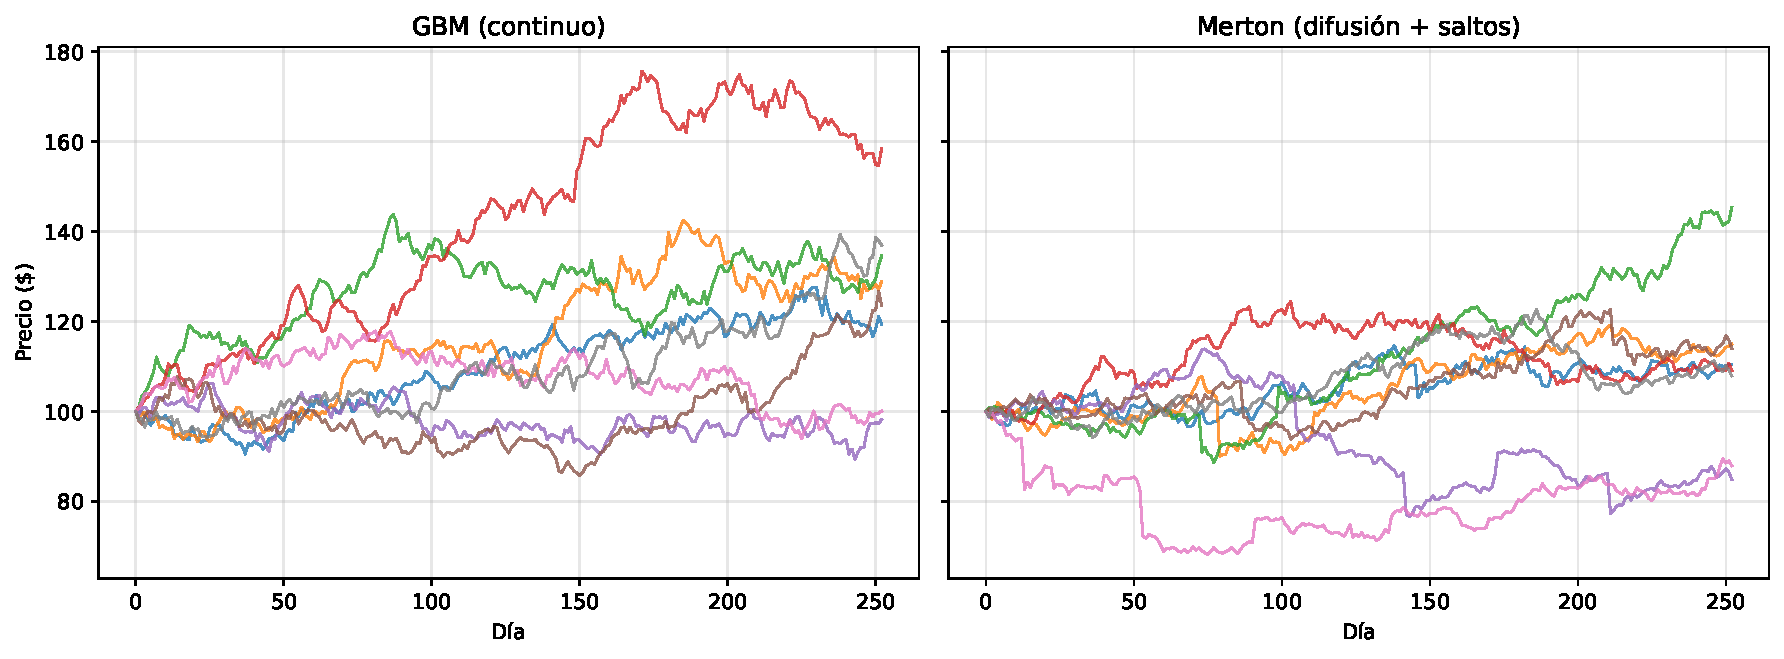
\includegraphics[keepaspectratio]{unidad3/cap14_procesos_estocasticos_activos_files/figure-pdf/merton-trayectorias-output-1.pdf}}

Se ve a simple vista: las trayectorias del GBM son ``peludas pero
suaves''; las de Merton muestran \textbf{escalones} --- el precio de
pronto está en otro lado, sin pasar por el medio. Así se ve un evento de
riesgo real.

\section{La firma en las
distribuciones}\label{la-firma-en-las-distribuciones}

La diferencia decisiva está en la distribución de los retornos:

\begin{Shaded}
\begin{Highlighting}[]
\NormalTok{ret\_m }\OperatorTok{=}\NormalTok{ np.log(S\_merton[}\OperatorTok{{-}}\DecValTok{1}\NormalTok{] }\OperatorTok{/}\NormalTok{ S0)}
\NormalTok{ret\_g }\OperatorTok{=}\NormalTok{ np.log(S\_gbm[}\OperatorTok{{-}}\DecValTok{1}\NormalTok{] }\OperatorTok{/}\NormalTok{ S0)}

\NormalTok{fig, ax }\OperatorTok{=}\NormalTok{ plt.subplots(figsize}\OperatorTok{=}\NormalTok{(}\DecValTok{9}\NormalTok{, }\DecValTok{5}\NormalTok{))}
\NormalTok{bins }\OperatorTok{=}\NormalTok{ np.linspace(}\BuiltInTok{min}\NormalTok{(ret\_m.}\BuiltInTok{min}\NormalTok{(), ret\_g.}\BuiltInTok{min}\NormalTok{()), }\BuiltInTok{max}\NormalTok{(ret\_m.}\BuiltInTok{max}\NormalTok{(), ret\_g.}\BuiltInTok{max}\NormalTok{()), }\DecValTok{80}\NormalTok{)}
\NormalTok{ax.hist(ret\_g, bins}\OperatorTok{=}\NormalTok{bins, density}\OperatorTok{=}\VariableTok{True}\NormalTok{, alpha}\OperatorTok{=}\FloatTok{0.55}\NormalTok{, label}\OperatorTok{=}\StringTok{"GBM"}\NormalTok{, color}\OperatorTok{=}\StringTok{"steelblue"}\NormalTok{)}
\NormalTok{ax.hist(ret\_m, bins}\OperatorTok{=}\NormalTok{bins, density}\OperatorTok{=}\VariableTok{True}\NormalTok{, alpha}\OperatorTok{=}\FloatTok{0.55}\NormalTok{, label}\OperatorTok{=}\StringTok{"Merton"}\NormalTok{, color}\OperatorTok{=}\StringTok{"indianred"}\NormalTok{)}
\NormalTok{ax.set\_yscale(}\StringTok{"log"}\NormalTok{)   }\CommentTok{\# escala log para VER las colas}
\NormalTok{ax.set\_xlabel(}\StringTok{"Retorno logarítmico a 1 año"}\NormalTok{)}
\NormalTok{ax.set\_ylabel(}\StringTok{"Densidad (escala log)"}\NormalTok{)}
\NormalTok{ax.set\_title(}\StringTok{"Misma volatilidad total, colas muy distintas"}\NormalTok{)}
\NormalTok{ax.legend()}
\NormalTok{ax.grid(}\VariableTok{True}\NormalTok{, alpha}\OperatorTok{=}\FloatTok{0.3}\NormalTok{)}
\NormalTok{plt.tight\_layout()}
\NormalTok{plt.show()}

\BuiltInTok{print}\NormalTok{(}\SpecialStringTok{f"}\SpecialCharTok{\{}\StringTok{\textquotesingle{}\textquotesingle{}}\SpecialCharTok{:24\}\{}\StringTok{\textquotesingle{}GBM\textquotesingle{}}\SpecialCharTok{:\textgreater{}10\}\{}\StringTok{\textquotesingle{}Merton\textquotesingle{}}\SpecialCharTok{:\textgreater{}10\}}\SpecialStringTok{"}\NormalTok{)}
\BuiltInTok{print}\NormalTok{(}\SpecialStringTok{f"}\SpecialCharTok{\{}\StringTok{\textquotesingle{}Asimetría\textquotesingle{}}\SpecialCharTok{:\textless{}24\}\{}\NormalTok{stats}\SpecialCharTok{.}\NormalTok{skew(ret\_g)}\SpecialCharTok{:\textgreater{}10.2f\}\{}\NormalTok{stats}\SpecialCharTok{.}\NormalTok{skew(ret\_m)}\SpecialCharTok{:\textgreater{}10.2f\}}\SpecialStringTok{"}\NormalTok{)}
\BuiltInTok{print}\NormalTok{(}\SpecialStringTok{f"}\SpecialCharTok{\{}\StringTok{\textquotesingle{}Curtosis (exceso)\textquotesingle{}}\SpecialCharTok{:\textless{}24\}\{}\NormalTok{stats}\SpecialCharTok{.}\NormalTok{kurtosis(ret\_g)}\SpecialCharTok{:\textgreater{}10.2f\}\{}\NormalTok{stats}\SpecialCharTok{.}\NormalTok{kurtosis(ret\_m)}\SpecialCharTok{:\textgreater{}10.2f\}}\SpecialStringTok{"}\NormalTok{)}
\BuiltInTok{print}\NormalTok{(}\SpecialStringTok{f"}\SpecialCharTok{\{}\StringTok{\textquotesingle{}Percentil 1\%\textquotesingle{}}\SpecialCharTok{:\textless{}24\}\{}\NormalTok{np}\SpecialCharTok{.}\NormalTok{percentile(ret\_g, }\DecValTok{1}\NormalTok{)}\SpecialCharTok{:\textgreater{}10.2\%\}\{}\NormalTok{np}\SpecialCharTok{.}\NormalTok{percentile(ret\_m, }\DecValTok{1}\NormalTok{)}\SpecialCharTok{:\textgreater{}10.2\%\}}\SpecialStringTok{"}\NormalTok{)}
\end{Highlighting}
\end{Shaded}

\pandocbounded{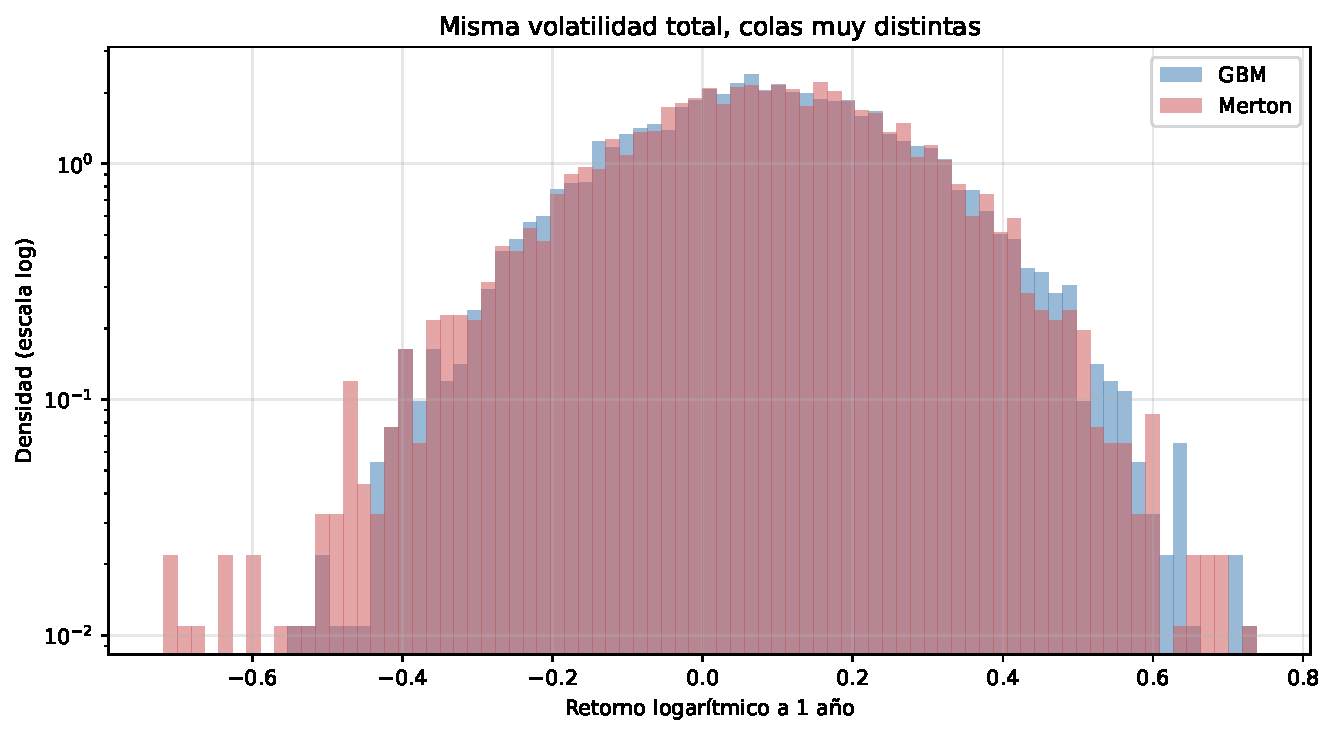
\includegraphics[keepaspectratio]{unidad3/cap14_procesos_estocasticos_activos_files/figure-pdf/merton-distribucion-output-1.pdf}}

\begin{verbatim}
                               GBM    Merton
Asimetría                     0.01     -0.19
Curtosis (exceso)            -0.09      0.22
Percentil 1%               -36.24%   -39.69%
\end{verbatim}

La escala logarítmica del eje y revela lo que el histograma común
esconde: la \textbf{cola izquierda de Merton se extiende mucho más
lejos} con probabilidad no despreciable. Ambos modelos tienen la misma
varianza --- un optimizador de Markowitz los vería idénticos --- pero el
VaR y el ES del 1\% son muy distintos. Esta es la materialización de la
lección de 2008 del capítulo anterior: \textbf{media y varianza no
cuentan la historia de las colas}.

\begin{center}\rule{0.5\linewidth}{0.5pt}\end{center}

\chapter{Procesos de Lévy: la familia
general}\label{procesos-de-luxe9vy-la-familia-general}

El Browniano y el Poisson comparten una propiedad estructural:
\textbf{incrementos independientes y estacionarios} (lo que pasa hoy no
depende de ayer, y las reglas del juego no cambian con el tiempo). La
familia completa de procesos con esa propiedad son los \textbf{procesos
de Lévy}, y hay un teorema hermoso (Lévy-Itô) que dice que \emph{todo}
proceso de Lévy se descompone en exactamente tres partes:

\[X_t = \underbrace{bt}_{\text{tendencia}} + \underbrace{\sigma W_t}_{\text{difusión}} + \underbrace{\text{saltos}}_{\text{grandes y pequeños}}\]

Es decir: \textbf{tendencia + Browniano + saltos es todo lo que puede
haber} (bajo incrementos independientes). El GBM usa solo las dos
primeras piezas; Merton agrega saltos ``raros y grandes''; y otros
miembros de la familia usados en la industria empujan la idea más lejos:

\begin{itemize}
\tightlist
\item
  \textbf{Variance Gamma (VG)}: infinitos saltos pequeños y ninguna
  difusión --- el precio se mueve \emph{solo} por saltitos. Se construye
  elegantemente como un Browniano evaluado en un ``reloj aleatorio''
  (subordinador Gamma): el tiempo del mercado corre más rápido en días
  agitados.
\item
  \textbf{Normal Inverse Gaussian (NIG)}, \textbf{CGMY}: variantes con
  más control fino sobre el peso de cada cola.
\end{itemize}

\phantomsection\label{variance-gamma}
\begin{Shaded}
\begin{Highlighting}[]
\CommentTok{\# Variance Gamma por subordinación: Browniano en "tiempo de mercado" aleatorio}
\KeywordTok{def}\NormalTok{ simular\_vg(theta, sigma\_vg, nu, T, n\_pasos, n\_sims, rng):}
    \CommentTok{"""Retornos log acumulados de un proceso Variance Gamma."""}
\NormalTok{    dt }\OperatorTok{=}\NormalTok{ T }\OperatorTok{/}\NormalTok{ n\_pasos}
    \CommentTok{\# El reloj aleatorio: incrementos Gamma con media dt y varianza nu*dt}
\NormalTok{    dG }\OperatorTok{=}\NormalTok{ rng.gamma(shape}\OperatorTok{=}\NormalTok{dt }\OperatorTok{/}\NormalTok{ nu, scale}\OperatorTok{=}\NormalTok{nu, size}\OperatorTok{=}\NormalTok{(n\_pasos, n\_sims))}
    \CommentTok{\# Browniano con drift evaluado en ese reloj}
\NormalTok{    dX }\OperatorTok{=}\NormalTok{ theta }\OperatorTok{*}\NormalTok{ dG }\OperatorTok{+}\NormalTok{ sigma\_vg }\OperatorTok{*}\NormalTok{ np.sqrt(dG) }\OperatorTok{*}\NormalTok{ rng.standard\_normal((n\_pasos, n\_sims))}
    \ControlFlowTok{return}\NormalTok{ dX.}\BuiltInTok{sum}\NormalTok{(axis}\OperatorTok{=}\DecValTok{0}\NormalTok{)}

\NormalTok{ret\_vg }\OperatorTok{=}\NormalTok{ simular\_vg(theta}\OperatorTok{={-}}\FloatTok{0.10}\NormalTok{, sigma\_vg}\OperatorTok{=}\FloatTok{0.18}\NormalTok{, nu}\OperatorTok{=}\FloatTok{0.4}\NormalTok{, T}\OperatorTok{=}\FloatTok{1.0}\NormalTok{,}
\NormalTok{                    n\_pasos}\OperatorTok{=}\DecValTok{252}\NormalTok{, n\_sims}\OperatorTok{=}\DecValTok{5000}\NormalTok{, rng}\OperatorTok{=}\NormalTok{rng)}

\BuiltInTok{print}\NormalTok{(}\StringTok{"Retornos a 1 año — Variance Gamma vs. GBM:"}\NormalTok{)}
\BuiltInTok{print}\NormalTok{(}\SpecialStringTok{f"}\SpecialCharTok{\{}\StringTok{\textquotesingle{}\textquotesingle{}}\SpecialCharTok{:24\}\{}\StringTok{\textquotesingle{}GBM\textquotesingle{}}\SpecialCharTok{:\textgreater{}10\}\{}\StringTok{\textquotesingle{}VG\textquotesingle{}}\SpecialCharTok{:\textgreater{}10\}}\SpecialStringTok{"}\NormalTok{)}
\BuiltInTok{print}\NormalTok{(}\SpecialStringTok{f"}\SpecialCharTok{\{}\StringTok{\textquotesingle{}Asimetría\textquotesingle{}}\SpecialCharTok{:\textless{}24\}\{}\NormalTok{stats}\SpecialCharTok{.}\NormalTok{skew(ret\_g)}\SpecialCharTok{:\textgreater{}10.2f\}\{}\NormalTok{stats}\SpecialCharTok{.}\NormalTok{skew(ret\_vg)}\SpecialCharTok{:\textgreater{}10.2f\}}\SpecialStringTok{"}\NormalTok{)}
\BuiltInTok{print}\NormalTok{(}\SpecialStringTok{f"}\SpecialCharTok{\{}\StringTok{\textquotesingle{}Curtosis (exceso)\textquotesingle{}}\SpecialCharTok{:\textless{}24\}\{}\NormalTok{stats}\SpecialCharTok{.}\NormalTok{kurtosis(ret\_g)}\SpecialCharTok{:\textgreater{}10.2f\}\{}\NormalTok{stats}\SpecialCharTok{.}\NormalTok{kurtosis(ret\_vg)}\SpecialCharTok{:\textgreater{}10.2f\}}\SpecialStringTok{"}\NormalTok{)}
\end{Highlighting}
\end{Shaded}

\begin{verbatim}
Retornos a 1 año — Variance Gamma vs. GBM:
                               GBM        VG
Asimetría                     0.01     -0.58
Curtosis (exceso)            -0.09      1.43
\end{verbatim}

\begin{tcolorbox}[enhanced jigsaw, bottomrule=.15mm, colback=white, opacitybacktitle=0.6, arc=.35mm, toprule=.15mm, opacityback=0, breakable, titlerule=0mm, left=2mm, coltitle=black, colbacktitle=quarto-callout-note-color!10!white, colframe=quarto-callout-note-color-frame, leftrule=.75mm, toptitle=1mm, bottomtitle=1mm, title=\textcolor{quarto-callout-note-color}{\faInfo}\hspace{0.5em}{¿Por qué molestarse con estos modelos?}, rightrule=.15mm]

Porque el uso profesional los exige en dos frentes. \textbf{Riesgo}: un
VaR/ES calculado con colas realistas (Capítulo 11 + este) es la
diferencia entre estar preparado o no. \textbf{Derivados}: las opciones
fuera del dinero cotizan ``caras'' respecto de Black-Scholes
precisamente porque el mercado \emph{sí} les pone precio a los saltos;
los modelos de Lévy reproducen ese patrón (la \emph{sonrisa} de
volatilidad, que formalizamos en el Módulo 4).

\end{tcolorbox}

\begin{center}\rule{0.5\linewidth}{0.5pt}\end{center}

\chapter{¿Qué modelo usar? Un mapa}\label{quuxe9-modelo-usar-un-mapa}

\begin{longtable}[]{@{}
  >{\raggedright\arraybackslash}p{(\linewidth - 8\tabcolsep) * \real{0.2000}}
  >{\raggedright\arraybackslash}p{(\linewidth - 8\tabcolsep) * \real{0.2000}}
  >{\raggedright\arraybackslash}p{(\linewidth - 8\tabcolsep) * \real{0.2000}}
  >{\raggedright\arraybackslash}p{(\linewidth - 8\tabcolsep) * \real{0.2000}}
  >{\raggedright\arraybackslash}p{(\linewidth - 8\tabcolsep) * \real{0.2000}}@{}}
\toprule\noalign{}
\begin{minipage}[b]{\linewidth}\raggedright
Modelo
\end{minipage} & \begin{minipage}[b]{\linewidth}\raggedright
Colas
\end{minipage} & \begin{minipage}[b]{\linewidth}\raggedright
Saltos
\end{minipage} & \begin{minipage}[b]{\linewidth}\raggedright
Costo
\end{minipage} & \begin{minipage}[b]{\linewidth}\raggedright
Cuándo usarlo
\end{minipage} \\
\midrule\noalign{}
\endhead
\bottomrule\noalign{}
\endlastfoot
\textbf{GBM} & Finas (normal) & No & Trivial & Primer boceto; horizontes
largos donde el promedio manda \\
\textbf{Merton} & Pesadas & Sí, raros y grandes & Bajo & Riesgo de
eventos; activos expuestos a anuncios/default \\
\textbf{Variance Gamma / NIG} & Pesadas, control fino & Infinitos,
pequeños & Medio & Calibración fina a opciones; alta frecuencia \\
\textbf{Heston / SABR} (Cap. 20) & Pesadas vía vol estocástica &
Opcional & Medio-alto & Superficies de volatilidad; pricing de
exóticos \\
\end{longtable}

La regla general del oficio: \textbf{el modelo correcto depende de la
pregunta}. Para proyectar la jubilación a 30 años, el GBM alcanza. Para
calcular el ES al 99\% de un book de opciones vendidas, usar GBM es
negligencia.

\begin{center}\rule{0.5\linewidth}{0.5pt}\end{center}

\chapter{Errores comunes}\label{errores-comunes-12}

\begin{tcolorbox}[enhanced jigsaw, bottomrule=.15mm, colback=white, opacitybacktitle=0.6, arc=.35mm, toprule=.15mm, opacityback=0, breakable, titlerule=0mm, left=2mm, coltitle=black, colbacktitle=quarto-callout-warning-color!10!white, colframe=quarto-callout-warning-color-frame, leftrule=.75mm, toptitle=1mm, bottomtitle=1mm, title=\textcolor{quarto-callout-warning-color}{\faExclamationTriangle}\hspace{0.5em}{Trampas frecuentes}, rightrule=.15mm]

\begin{itemize}
\tightlist
\item
  \textbf{Olvidar el compensador} (\(-\lambda k\, dt\)) en Merton: sin
  él, los saltos negativos sesgan el drift y la media simulada no
  coincide con la teórica.
\item
  \textbf{Calibrar los saltos con datos tranquilos}: si la muestra
  histórica no contiene crisis, el estimador de \(\lambda\) será
  \textasciitilde0 y el modelo degenera en GBM. Los parámetros de salto
  suelen calibrarse con opciones (forward-looking), no solo con
  historia.
\item
  \textbf{Comparar modelos con distinta varianza total}: para aislar el
  efecto de \emph{forma} (colas, asimetría), igualá la varianza como
  hicimos acá; si no, confundís ``más riesgo'' con ``riesgo distinto''.
\item
  \textbf{Confundir curtosis muestral con poblacional}: la curtosis
  estimada con pocas observaciones de un proceso con saltos es
  tremendamente ruidosa (¡depende de cuántos saltos cayeron en tu
  muestra!).
\end{itemize}

\end{tcolorbox}

\begin{center}\rule{0.5\linewidth}{0.5pt}\end{center}

\chapter{Ejercicios Propuestos}\label{ejercicios-propuestos-13}

\begin{tcolorbox}[enhanced jigsaw, bottomrule=.15mm, colback=white, opacitybacktitle=0.6, arc=.35mm, toprule=.15mm, opacityback=0, breakable, titlerule=0mm, left=2mm, coltitle=black, colbacktitle=quarto-callout-important-color!10!white, colframe=quarto-callout-important-color-frame, leftrule=.75mm, toptitle=1mm, bottomtitle=1mm, title=\textcolor{quarto-callout-important-color}{\faExclamation}\hspace{0.5em}{Ejercicios}, rightrule=.15mm]

\begin{enumerate}
\def\labelenumi{\arabic{enumi}.}
\tightlist
\item
  \textbf{ES bajo saltos}: calculá el Expected Shortfall al 99\% a 1 año
  bajo GBM y bajo Merton (misma varianza total). ¿Qué error porcentual
  comete el GBM?
\item
  \textbf{Sensibilidad a λ}: barré \(\lambda \in \{1, 4, 12\}\)
  (manteniendo la varianza total constante ajustando \(\sigma\)) y
  graficá la curtosis de los retornos resultantes.
\item
  \textbf{Detección de saltos}: con los retornos diarios simulados de
  Merton, proponé una regla simple para detectar los días de salto
  (p.~ej., \(|r| > 4\sigma_{\text{difusión}}\)) y medí su tasa de
  aciertos contra los saltos verdaderos.
\item
  \textbf{Datos reales}: bajá 10 años de retornos diarios de un índice,
  calculá asimetría, curtosis y el peor día, y compará contra lo que
  produce un GBM calibrado a su media y varianza. ¿Cuántos ``días
  imposibles'' (\textgreater4σ) encontrás?
\item
  \textbf{VG vs.~Merton}: superponé los histogramas (en escala log) de
  retornos a 1 año de VG y Merton calibrados a la misma varianza. ¿En
  qué se diferencian sus colas?
\end{enumerate}

\end{tcolorbox}

Podés resolver estos ejercicios acá mismo: la celda ejecuta Python
\textbf{en tu navegador}, sin instalar nada (la primera ejecución tarda
unos segundos mientras carga el entorno; los paquetes que importes se
instalan solos).

\begin{Shaded}
\begin{Highlighting}[]
\NormalTok{\#| label: practica{-}navegador}
\NormalTok{import numpy as np}

\NormalTok{rng = np.random.default\_rng(42)}

\NormalTok{\# Tu solución acá...}
\end{Highlighting}
\end{Shaded}

\begin{center}\rule{0.5\linewidth}{0.5pt}\end{center}

\chapter{Referencias}\label{referencias-13}

\phantomsection\label{refs}

\chapter{Capítulo 15: Econometría y Modelos Lineales en
Finanzas}\label{capuxedtulo-15-econometruxeda-y-modelos-lineales-en-finanzas}

De la regresión simple a los modelos multifactor

La regresión lineal es la herramienta más usada de las finanzas
cuantitativas: con ella se estiman betas, se construyen coberturas, se
descomponen retornos en factores y se testean estrategias. Este capítulo
la desarrolla en serio: cómo especificar un modelo, qué supuestos lo
sostienen, cómo leer coeficientes, errores estándar y p-values, y cómo
aplicarla al CAPM, a los modelos multifactor y al cálculo de ratios de
cobertura. Implementamos MCO desde cero y con statsmodels.

\hfill\break

\chapter{Introducción}\label{introducciuxf3n-12}

Si tuvieras que quedarte con una sola herramienta estadística para
trabajar en finanzas, sería la \textbf{regresión lineal}. Con ella se
responde una familia enorme de preguntas que comparten la misma
estructura: \emph{¿cómo se mueve \(y\) cuando se mueve \(x\)?}

\begin{itemize}
\tightlist
\item
  ¿Cuánto cae mi acción cuando cae el mercado? (beta del CAPM)
\item
  ¿Cuántos futuros necesito vender para cubrir mi cartera? (ratio de
  cobertura)
\item
  ¿Mi fondo genera valor o solo cobra caro por exposición al mercado?
  (alfa)
\item
  ¿Qué parte del retorno se explica por tamaño, valor, momentum?
  (modelos de factores)
\end{itemize}

Este capítulo construye la herramienta con el rigor necesario para
usarla bien: no alcanza con llamar a una librería; hay que saber
\textbf{qué supone el modelo, cuándo mienten los p-values y cómo se leen
los resultados}.

\phantomsection\label{setup}
\begin{Shaded}
\begin{Highlighting}[]
\ImportTok{import}\NormalTok{ numpy }\ImportTok{as}\NormalTok{ np}
\ImportTok{import}\NormalTok{ pandas }\ImportTok{as}\NormalTok{ pd}
\ImportTok{import}\NormalTok{ matplotlib.pyplot }\ImportTok{as}\NormalTok{ plt}
\ImportTok{from}\NormalTok{ scipy }\ImportTok{import}\NormalTok{ stats}
\ImportTok{import}\NormalTok{ statsmodels.api }\ImportTok{as}\NormalTok{ sm}

\NormalTok{rng }\OperatorTok{=}\NormalTok{ np.random.default\_rng(}\DecValTok{42}\NormalTok{)}
\end{Highlighting}
\end{Shaded}

\begin{center}\rule{0.5\linewidth}{0.5pt}\end{center}

\chapter{El modelo lineal: qué afirma
exactamente}\label{el-modelo-lineal-quuxe9-afirma-exactamente}

El modelo de regresión lineal postula que la variable a explicar \(y\)
es una combinación lineal de las explicativas más un término de error:

\[y_i = \beta_0 + \beta_1 x_{1i} + \beta_2 x_{2i} + \dots + \beta_k x_{ki} + \varepsilon_i\]

Tres aclaraciones que evitan malentendidos comunes:

\begin{enumerate}
\def\labelenumi{\arabic{enumi}.}
\tightlist
\item
  \textbf{``Lineal'' es en los coeficientes, no en las variables.}
  \(y = \beta_0 + \beta_1 x^2\) es un modelo lineal perfectamente
  válido; podés transformar las variables como quieras.
\item
  \textbf{El error \(\varepsilon\) no es un defecto}: representa todo lo
  que afecta a \(y\) y no está en el modelo. La pregunta clave será qué
  propiedades tiene.
\item
  \textbf{Los \(\beta\) se interpretan ``todo lo demás constante''}:
  \(\beta_1\) es el efecto de \(x_1\) sobre \(y\) \emph{manteniendo
  fijas las otras variables}. Esta lectura condicional es lo que hace
  potente (y delicada) a la regresión múltiple.
\end{enumerate}

\section{Estimación por Mínimos Cuadrados Ordinarios
(MCO)}\label{estimaciuxf3n-por-muxednimos-cuadrados-ordinarios-mco}

¿Cómo elegir los \(\beta\)? El criterio de \textbf{MCO} (\emph{OLS} en
inglés): minimizar la suma de los errores al cuadrado. Para el caso
simple (\(y = \alpha + \beta x + \varepsilon\)) la solución tiene forma
cerrada:

\[\hat\beta = \frac{\text{Cov}(x, y)}{\text{Var}(x)}, \qquad \hat\alpha = \bar{y} - \hat\beta \bar{x}\]

La primera fórmula es reveladora: \textbf{el beta es una covarianza
normalizada}. Ya la conocés de la teoría de portafolios --- no es
casualidad, es la misma matemática.

Implementémosla desde cero para desmitificarla:

\phantomsection\label{clase-regresion}
\begin{Shaded}
\begin{Highlighting}[]
\KeywordTok{class}\NormalTok{ RegresionLineal:}
    \CommentTok{"""Regresión lineal simple por MCO, implementada desde cero."""}

    \KeywordTok{def}\NormalTok{ fit(}\VariableTok{self}\NormalTok{, x, y):}
\NormalTok{        x, y }\OperatorTok{=}\NormalTok{ np.asarray(x), np.asarray(y)}
        \VariableTok{self}\NormalTok{.n }\OperatorTok{=} \BuiltInTok{len}\NormalTok{(x)}
\NormalTok{        x\_mean, y\_mean }\OperatorTok{=}\NormalTok{ x.mean(), y.mean()}

        \CommentTok{\# Estimadores MCO}
        \VariableTok{self}\NormalTok{.beta }\OperatorTok{=}\NormalTok{ np.}\BuiltInTok{sum}\NormalTok{((x }\OperatorTok{{-}}\NormalTok{ x\_mean) }\OperatorTok{*}\NormalTok{ (y }\OperatorTok{{-}}\NormalTok{ y\_mean)) }\OperatorTok{/}\NormalTok{ np.}\BuiltInTok{sum}\NormalTok{((x }\OperatorTok{{-}}\NormalTok{ x\_mean) }\OperatorTok{**} \DecValTok{2}\NormalTok{)}
        \VariableTok{self}\NormalTok{.alpha }\OperatorTok{=}\NormalTok{ y\_mean }\OperatorTok{{-}} \VariableTok{self}\NormalTok{.beta }\OperatorTok{*}\NormalTok{ x\_mean}

        \CommentTok{\# Bondad de ajuste y errores estándar}
\NormalTok{        y\_hat }\OperatorTok{=} \VariableTok{self}\NormalTok{.alpha }\OperatorTok{+} \VariableTok{self}\NormalTok{.beta }\OperatorTok{*}\NormalTok{ x}
\NormalTok{        residuos }\OperatorTok{=}\NormalTok{ y }\OperatorTok{{-}}\NormalTok{ y\_hat}
\NormalTok{        ss\_res }\OperatorTok{=}\NormalTok{ np.}\BuiltInTok{sum}\NormalTok{(residuos }\OperatorTok{**} \DecValTok{2}\NormalTok{)}
\NormalTok{        ss\_tot }\OperatorTok{=}\NormalTok{ np.}\BuiltInTok{sum}\NormalTok{((y }\OperatorTok{{-}}\NormalTok{ y\_mean) }\OperatorTok{**} \DecValTok{2}\NormalTok{)}
        \VariableTok{self}\NormalTok{.r2 }\OperatorTok{=} \DecValTok{1} \OperatorTok{{-}}\NormalTok{ ss\_res }\OperatorTok{/}\NormalTok{ ss\_tot}

        \CommentTok{\# Error estándar del beta y test t (H0: beta = 0)}
\NormalTok{        s2 }\OperatorTok{=}\NormalTok{ ss\_res }\OperatorTok{/}\NormalTok{ (}\VariableTok{self}\NormalTok{.n }\OperatorTok{{-}} \DecValTok{2}\NormalTok{)                       }\CommentTok{\# varianza residual}
        \VariableTok{self}\NormalTok{.se\_beta }\OperatorTok{=}\NormalTok{ np.sqrt(s2 }\OperatorTok{/}\NormalTok{ np.}\BuiltInTok{sum}\NormalTok{((x }\OperatorTok{{-}}\NormalTok{ x\_mean) }\OperatorTok{**} \DecValTok{2}\NormalTok{))}
        \VariableTok{self}\NormalTok{.t\_beta }\OperatorTok{=} \VariableTok{self}\NormalTok{.beta }\OperatorTok{/} \VariableTok{self}\NormalTok{.se\_beta}
        \VariableTok{self}\NormalTok{.p\_beta }\OperatorTok{=} \DecValTok{2} \OperatorTok{*}\NormalTok{ (}\DecValTok{1} \OperatorTok{{-}}\NormalTok{ stats.t.cdf(}\BuiltInTok{abs}\NormalTok{(}\VariableTok{self}\NormalTok{.t\_beta), df}\OperatorTok{=}\VariableTok{self}\NormalTok{.n }\OperatorTok{{-}} \DecValTok{2}\NormalTok{))}
        \ControlFlowTok{return} \VariableTok{self}

    \KeywordTok{def}\NormalTok{ resumen(}\VariableTok{self}\NormalTok{):}
        \BuiltInTok{print}\NormalTok{(}\SpecialStringTok{f"alpha = }\SpecialCharTok{\{}\VariableTok{self}\SpecialCharTok{.}\NormalTok{alpha}\SpecialCharTok{:.6f\}}\SpecialStringTok{"}\NormalTok{)}
        \BuiltInTok{print}\NormalTok{(}\SpecialStringTok{f"beta  = }\SpecialCharTok{\{}\VariableTok{self}\SpecialCharTok{.}\NormalTok{beta}\SpecialCharTok{:.4f\}}\SpecialStringTok{  (se: }\SpecialCharTok{\{}\VariableTok{self}\SpecialCharTok{.}\NormalTok{se\_beta}\SpecialCharTok{:.4f\}}\SpecialStringTok{, "}
              \SpecialStringTok{f"t: }\SpecialCharTok{\{}\VariableTok{self}\SpecialCharTok{.}\NormalTok{t\_beta}\SpecialCharTok{:.2f\}}\SpecialStringTok{, p{-}value: }\SpecialCharTok{\{}\VariableTok{self}\SpecialCharTok{.}\NormalTok{p\_beta}\SpecialCharTok{:.4f\}}\SpecialStringTok{)"}\NormalTok{)}
        \BuiltInTok{print}\NormalTok{(}\SpecialStringTok{f"R²    = }\SpecialCharTok{\{}\VariableTok{self}\SpecialCharTok{.}\NormalTok{r2}\SpecialCharTok{:.4f\}}\SpecialStringTok{"}\NormalTok{)}
\end{Highlighting}
\end{Shaded}

\begin{center}\rule{0.5\linewidth}{0.5pt}\end{center}

\chapter{Aplicación 1: el CAPM y la estimación del
beta}\label{aplicaciuxf3n-1-el-capm-y-la-estimaciuxf3n-del-beta}

El \textbf{CAPM} (Capital Asset Pricing Model) afirma que el exceso de
retorno esperado de un activo es proporcional al exceso de retorno del
mercado:

\[E[R_i] - r_f = \beta_i \left(E[R_m] - r_f\right)\]

Su versión empírica es una regresión lineal sobre datos históricos:

\[\underbrace{R_{i,t} - r_f}_{y} = \alpha + \beta \underbrace{(R_{m,t} - r_f)}_{x} + \varepsilon_t\]

\begin{itemize}
\tightlist
\item
  \(\beta\) mide la \textbf{sensibilidad al mercado}: β=1.3 significa
  ``cuando el mercado sube 1\%, este activo sube 1.3\% en promedio''.
\item
  \(\alpha\) es el retorno \textbf{no explicado por el mercado}: si es
  positivo y significativo, el activo rindió más de lo que su riesgo
  justifica. Todo gestor activo afirma tener alfa; la regresión permite
  verificarlo.
\end{itemize}

\phantomsection\label{capm}
\begin{Shaded}
\begin{Highlighting}[]
\CommentTok{\# Simulamos 10 años de datos mensuales con parámetros conocidos}
\NormalTok{n }\OperatorTok{=} \DecValTok{120}
\NormalTok{beta\_real, alpha\_real }\OperatorTok{=} \FloatTok{1.3}\NormalTok{, }\FloatTok{0.002}

\NormalTok{exceso\_mercado }\OperatorTok{=}\NormalTok{ rng.normal(}\FloatTok{0.005}\NormalTok{, }\FloatTok{0.04}\NormalTok{, n)}
\NormalTok{exceso\_activo }\OperatorTok{=}\NormalTok{ alpha\_real }\OperatorTok{+}\NormalTok{ beta\_real }\OperatorTok{*}\NormalTok{ exceso\_mercado }\OperatorTok{+}\NormalTok{ rng.normal(}\DecValTok{0}\NormalTok{, }\FloatTok{0.03}\NormalTok{, n)}

\NormalTok{modelo }\OperatorTok{=}\NormalTok{ RegresionLineal().fit(exceso\_mercado, exceso\_activo)}
\BuiltInTok{print}\NormalTok{(}\StringTok{"=== CAPM estimado (desde cero) ==="}\NormalTok{)}
\NormalTok{modelo.resumen()}
\BuiltInTok{print}\NormalTok{(}\SpecialStringTok{f"}\CharTok{\textbackslash{}n}\SpecialStringTok{Valores reales: alpha=}\SpecialCharTok{\{}\NormalTok{alpha\_real}\SpecialCharTok{\}}\SpecialStringTok{, beta=}\SpecialCharTok{\{}\NormalTok{beta\_real}\SpecialCharTok{\}}\SpecialStringTok{"}\NormalTok{)}
\end{Highlighting}
\end{Shaded}

\begin{verbatim}
=== CAPM estimado (desde cero) ===
alpha = 0.001308
beta  = 1.1774  (se: 0.0878, t: 13.41, p-value: 0.0000)
R²    = 0.6038

Valores reales: alpha=0.002, beta=1.3
\end{verbatim}

El beta se recupera con precisión; el alfa, no tanto (mirá su p-value en
la salida de \texttt{statsmodels} más abajo). Esa asimetría no es un
accidente de esta muestra, es una lección general: \textbf{detectar alfa
exige muchísimos más datos que estimar beta}, porque el alfa es una
constante pequeña escondida en mucho ruido.

\begin{Shaded}
\begin{Highlighting}[]
\NormalTok{fig, ax }\OperatorTok{=}\NormalTok{ plt.subplots(figsize}\OperatorTok{=}\NormalTok{(}\DecValTok{8}\NormalTok{, }\DecValTok{5}\NormalTok{))}
\NormalTok{ax.scatter(exceso\_mercado }\OperatorTok{*} \DecValTok{100}\NormalTok{, exceso\_activo }\OperatorTok{*} \DecValTok{100}\NormalTok{, alpha}\OperatorTok{=}\FloatTok{0.5}\NormalTok{, s}\OperatorTok{=}\DecValTok{25}\NormalTok{)}
\NormalTok{x\_line }\OperatorTok{=}\NormalTok{ np.linspace(exceso\_mercado.}\BuiltInTok{min}\NormalTok{(), exceso\_mercado.}\BuiltInTok{max}\NormalTok{(), }\DecValTok{50}\NormalTok{)}
\NormalTok{ax.plot(x\_line }\OperatorTok{*} \DecValTok{100}\NormalTok{, (modelo.alpha }\OperatorTok{+}\NormalTok{ modelo.beta }\OperatorTok{*}\NormalTok{ x\_line) }\OperatorTok{*} \DecValTok{100}\NormalTok{, }\StringTok{"r{-}"}\NormalTok{,}
\NormalTok{        linewidth}\OperatorTok{=}\DecValTok{2}\NormalTok{, label}\OperatorTok{=}\SpecialStringTok{f"Recta MCO: β = }\SpecialCharTok{\{}\NormalTok{modelo}\SpecialCharTok{.}\NormalTok{beta}\SpecialCharTok{:.2f\}}\SpecialStringTok{"}\NormalTok{)}
\NormalTok{ax.set\_xlabel(}\StringTok{"Exceso de retorno del mercado (\%)"}\NormalTok{)}
\NormalTok{ax.set\_ylabel(}\StringTok{"Exceso de retorno del activo (\%)"}\NormalTok{)}
\NormalTok{ax.set\_title(}\SpecialStringTok{f"Security Characteristic Line — R² = }\SpecialCharTok{\{}\NormalTok{modelo}\SpecialCharTok{.}\NormalTok{r2}\SpecialCharTok{:.2f\}}\SpecialStringTok{"}\NormalTok{)}
\NormalTok{ax.legend()}
\NormalTok{ax.grid(}\VariableTok{True}\NormalTok{, alpha}\OperatorTok{=}\FloatTok{0.3}\NormalTok{)}
\NormalTok{plt.tight\_layout()}
\NormalTok{plt.show()}
\end{Highlighting}
\end{Shaded}

\pandocbounded{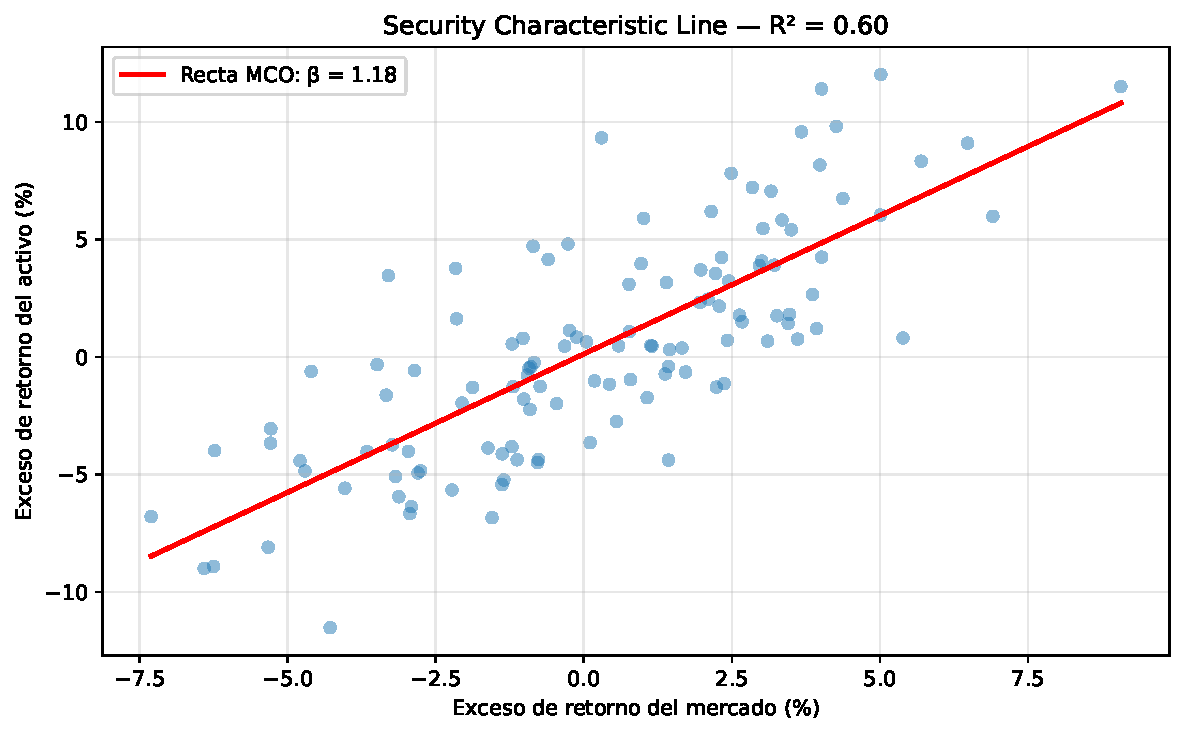
\includegraphics[keepaspectratio]{unidad3/cap15_econometria_modelos_lineales_files/figure-pdf/capm-grafico-output-1.pdf}}

\begin{center}\rule{0.5\linewidth}{0.5pt}\end{center}

\chapter{Leer una regresión: errores estándar, t y
p-values}\label{leer-una-regresiuxf3n-errores-estuxe1ndar-t-y-p-values}

Los coeficientes estimados son \textbf{variables aleatorias}: con otra
muestra habrían dado distinto. La inferencia estadística cuantifica esa
incertidumbre, y saber leerla es lo que separa un análisis serio de uno
decorativo.

\begin{itemize}
\tightlist
\item
  \textbf{Error estándar (se)}: el ``desvío típico'' del estimador. Un
  beta de 1.30 con se de 0.07 está bien clavado; con se de 0.60 no sabés
  casi nada.
\item
  \textbf{Estadístico t}: cuántos errores estándar dista el coeficiente
  de cero: \(t = \hat\beta / se(\hat\beta)\). Regla mental: \(|t| > 2\)
  ≈ significativo al 5\%.
\item
  \textbf{p-value}: la probabilidad de observar un coeficiente tan
  grande (en valor absoluto) \textbf{si el verdadero fuera cero}. Un
  p-value de 0.03 dice: ``si el activo no tuviera relación con el
  mercado, ver este beta sería raro (3\%)''.
\end{itemize}

\begin{tcolorbox}[enhanced jigsaw, bottomrule=.15mm, colback=white, opacitybacktitle=0.6, arc=.35mm, toprule=.15mm, opacityback=0, breakable, titlerule=0mm, left=2mm, coltitle=black, colbacktitle=quarto-callout-warning-color!10!white, colframe=quarto-callout-warning-color-frame, leftrule=.75mm, toptitle=1mm, bottomtitle=1mm, title=\textcolor{quarto-callout-warning-color}{\faExclamationTriangle}\hspace{0.5em}{Lo que el p-value NO dice}, rightrule=.15mm]

El p-value \textbf{no} es ``la probabilidad de que el coeficiente sea
cero'', ni ``la probabilidad de que el modelo esté mal''. Es una
afirmación sobre los \emph{datos bajo una hipótesis}, no sobre la
hipótesis. Y con miles de datos, coeficientes económicamente
irrelevantes se vuelven ``significativos'': \textbf{significancia
estadística ≠ relevancia económica}. Mirá siempre la magnitud del
coeficiente además de su p-value. Esta distinción reaparecerá con fuerza
en el Capítulo 17 (backtesting), donde probar muchas estrategias infla
los falsos positivos.

\end{tcolorbox}

\section{La versión profesional:
statsmodels}\label{la-versiuxf3n-profesional-statsmodels}

Nuestra clase enseña la mecánica; para trabajar en serio usamos
\texttt{statsmodels}, que reporta toda la inferencia de una vez:

\phantomsection\label{statsmodels}
\begin{Shaded}
\begin{Highlighting}[]
\NormalTok{X }\OperatorTok{=}\NormalTok{ sm.add\_constant(exceso\_mercado)     }\CommentTok{\# agrega la columna del intercepto}
\NormalTok{ols }\OperatorTok{=}\NormalTok{ sm.OLS(exceso\_activo, X).fit()}
\BuiltInTok{print}\NormalTok{(ols.summary(xname}\OperatorTok{=}\NormalTok{[}\StringTok{"alpha"}\NormalTok{, }\StringTok{"beta\_mkt"}\NormalTok{]))}
\end{Highlighting}
\end{Shaded}

\begin{verbatim}
                            OLS Regression Results                            
==============================================================================
Dep. Variable:                      y   R-squared:                       0.604
Model:                            OLS   Adj. R-squared:                  0.600
Method:                 Least Squares   F-statistic:                     179.8
Date:                Tue, 14 Jul 2026   Prob (F-statistic):           1.77e-25
Time:                        20:07:22   Log-Likelihood:                 251.24
No. Observations:                 120   AIC:                            -498.5
Df Residuals:                     118   BIC:                            -492.9
Df Model:                           1                                         
Covariance Type:            nonrobust                                         
==============================================================================
                 coef    std err          t      P>|t|      [0.025      0.975]
------------------------------------------------------------------------------
alpha          0.0013      0.003      0.475      0.636      -0.004       0.007
beta_mkt       1.1774      0.088     13.410      0.000       1.004       1.351
==============================================================================
Omnibus:                        3.957   Durbin-Watson:                   1.575
Prob(Omnibus):                  0.138   Jarque-Bera (JB):                3.816
Skew:                           0.436   Prob(JB):                        0.148
Kurtosis:                       2.946   Cond. No.                         32.0
==============================================================================

Notes:
[1] Standard Errors assume that the covariance matrix of the errors is correctly specified.
\end{verbatim}

De esta tabla, lo que hay que saber mirar: los \textbf{coeficientes} con
sus intervalos de confianza (¿el intervalo del beta contiene 1? ¿el del
alfa contiene 0?), el \textbf{R²} (proporción de la varianza explicada),
y los p-values. El resto (Durbin-Watson, Jarque-Bera de los residuos)
son diagnósticos de supuestos --- el tema siguiente.

\begin{center}\rule{0.5\linewidth}{0.5pt}\end{center}

\chapter{Los supuestos: cuándo confiar en
MCO}\label{los-supuestos-cuuxe1ndo-confiar-en-mco}

Los estimadores MCO son insesgados y de mínima varianza (\textbf{teorema
de Gauss-Markov}) cuando se cumplen ciertos supuestos. En finanzas,
algunos se violan sistemáticamente, y conviene saber cuáles y qué hacer:

\begin{longtable}[]{@{}
  >{\raggedright\arraybackslash}p{(\linewidth - 6\tabcolsep) * \real{0.2500}}
  >{\raggedright\arraybackslash}p{(\linewidth - 6\tabcolsep) * \real{0.2500}}
  >{\raggedright\arraybackslash}p{(\linewidth - 6\tabcolsep) * \real{0.2500}}
  >{\raggedright\arraybackslash}p{(\linewidth - 6\tabcolsep) * \real{0.2500}}@{}}
\toprule\noalign{}
\begin{minipage}[b]{\linewidth}\raggedright
Supuesto
\end{minipage} & \begin{minipage}[b]{\linewidth}\raggedright
Qué significa
\end{minipage} & \begin{minipage}[b]{\linewidth}\raggedright
¿Se cumple en finanzas?
\end{minipage} & \begin{minipage}[b]{\linewidth}\raggedright
Remedio usual
\end{minipage} \\
\midrule\noalign{}
\endhead
\bottomrule\noalign{}
\endlastfoot
Linealidad & La relación es lineal en los β & Aproximadamente &
Transformar variables \\
Exogeneidad & El error no está correlacionado con las x & El más
delicado & Diseño / variables instrumentales \\
Homocedasticidad & Varianza del error constante & \textbf{No} (la
volatilidad se agrupa) & Errores robustos (HC/HAC) \\
No autocorrelación & Errores independientes en el tiempo & \textbf{A
veces no} & Errores Newey-West (HAC) \\
Normalidad & Errores normales (para inferencia exacta) & No en colas &
Muestras grandes ayudan (TCL) \\
\end{longtable}

Las violaciones de homocedasticidad y autocorrelación \textbf{no sesgan
los coeficientes}, pero \textbf{mienten los errores estándar} --- y con
ellos los p-values. La solución estándar en finanzas es usar errores
robustos:

\phantomsection\label{errores-robustos}
\begin{Shaded}
\begin{Highlighting}[]
\CommentTok{\# Mismos coeficientes, errores estándar robustos a heterocedasticidad y autocorrelación}
\NormalTok{ols\_robusto }\OperatorTok{=}\NormalTok{ sm.OLS(exceso\_activo, X).fit(cov\_type}\OperatorTok{=}\StringTok{"HAC"}\NormalTok{, cov\_kwds}\OperatorTok{=}\NormalTok{\{}\StringTok{"maxlags"}\NormalTok{: }\DecValTok{6}\NormalTok{\})}

\BuiltInTok{print}\NormalTok{(}\StringTok{"Comparación de errores estándar del beta:"}\NormalTok{)}
\BuiltInTok{print}\NormalTok{(}\SpecialStringTok{f"  Clásico (asume homocedasticidad): }\SpecialCharTok{\{}\NormalTok{ols}\SpecialCharTok{.}\NormalTok{bse[}\DecValTok{1}\NormalTok{]}\SpecialCharTok{:.4f\}}\SpecialStringTok{"}\NormalTok{)}
\BuiltInTok{print}\NormalTok{(}\SpecialStringTok{f"  Robusto (Newey{-}West, HAC):        }\SpecialCharTok{\{}\NormalTok{ols\_robusto}\SpecialCharTok{.}\NormalTok{bse[}\DecValTok{1}\NormalTok{]}\SpecialCharTok{:.4f\}}\SpecialStringTok{"}\NormalTok{)}
\end{Highlighting}
\end{Shaded}

\begin{verbatim}
Comparación de errores estándar del beta:
  Clásico (asume homocedasticidad): 0.0878
  Robusto (Newey-West, HAC):        0.0794
\end{verbatim}

\begin{tcolorbox}[enhanced jigsaw, bottomrule=.15mm, colback=white, opacitybacktitle=0.6, arc=.35mm, toprule=.15mm, opacityback=0, breakable, titlerule=0mm, left=2mm, coltitle=black, colbacktitle=quarto-callout-tip-color!10!white, colframe=quarto-callout-tip-color-frame, leftrule=.75mm, toptitle=1mm, bottomtitle=1mm, title=\textcolor{quarto-callout-tip-color}{\faLightbulb}\hspace{0.5em}{Regla práctica}, rightrule=.15mm]

En regresiones con series de tiempo financieras, reportá errores
\textbf{Newey-West (HAC)} por defecto. Si los datos fueran ideales, no
perdés nada; si no lo son (lo usual), tus p-values dejan de estar
inflados.

\end{tcolorbox}

\begin{center}\rule{0.5\linewidth}{0.5pt}\end{center}

\chapter{Regresión múltiple: más de una
explicativa}\label{regresiuxf3n-muxfaltiple-muxe1s-de-una-explicativa}

La extensión a varias variables es directa en la práctica
(\texttt{statsmodels} recibe una matriz en lugar de un vector) pero
cambia la \textbf{interpretación}: cada coeficiente mide el efecto de su
variable \emph{controlando por las demás}. Esto permite responder
preguntas imposibles para la regresión simple: \emph{¿este fondo tiene
alfa, o su ``alfa'' es en realidad exposición a las acciones pequeñas?}

\section{Aplicación 2: modelos multifactor
(Fama-French)}\label{aplicaciuxf3n-2-modelos-multifactor-fama-french}

El CAPM explica los retornos con un solo factor (el mercado). La
evidencia empírica encontró sistemáticamente dos anomalías: las empresas
\textbf{chicas} rinden más que las grandes, y las \textbf{baratas} (alto
valor libro / valor de mercado) más que las caras. Fama y French (1993)
propusieron agregarlas como factores:

\[R_i - r_f = \alpha + \beta_m (R_m - r_f) + \beta_s \cdot SMB + \beta_v \cdot HML + \varepsilon\]

donde \textbf{SMB} (\emph{Small Minus Big}) es el retorno de las chicas
menos las grandes, y \textbf{HML} (\emph{High Minus Low}) el de las
baratas menos las caras.

\phantomsection\label{fama-french}
\begin{Shaded}
\begin{Highlighting}[]
\CommentTok{\# Simulamos los tres factores y un fondo con exposiciones conocidas}
\NormalTok{n }\OperatorTok{=} \DecValTok{240}   \CommentTok{\# 20 años de datos mensuales}
\NormalTok{mkt }\OperatorTok{=}\NormalTok{ rng.normal(}\FloatTok{0.005}\NormalTok{, }\FloatTok{0.040}\NormalTok{, n)}
\NormalTok{smb }\OperatorTok{=}\NormalTok{ rng.normal(}\FloatTok{0.001}\NormalTok{, }\FloatTok{0.025}\NormalTok{, n)}
\NormalTok{hml }\OperatorTok{=}\NormalTok{ rng.normal(}\FloatTok{0.002}\NormalTok{, }\FloatTok{0.025}\NormalTok{, n)}

\CommentTok{\# Un fondo "value con sesgo small": expuesto a los tres factores, sin alfa real}
\NormalTok{ret\_fondo }\OperatorTok{=} \FloatTok{0.0} \OperatorTok{+} \FloatTok{1.1} \OperatorTok{*}\NormalTok{ mkt }\OperatorTok{+} \FloatTok{0.5} \OperatorTok{*}\NormalTok{ smb }\OperatorTok{+} \FloatTok{0.7} \OperatorTok{*}\NormalTok{ hml }\OperatorTok{+}\NormalTok{ rng.normal(}\DecValTok{0}\NormalTok{, }\FloatTok{0.02}\NormalTok{, n)}

\CommentTok{\# Regresión CAPM (solo mercado) vs. modelo de 3 factores}
\NormalTok{X1 }\OperatorTok{=}\NormalTok{ sm.add\_constant(mkt)}
\NormalTok{X3 }\OperatorTok{=}\NormalTok{ sm.add\_constant(np.column\_stack([mkt, smb, hml]))}

\NormalTok{capm\_fit }\OperatorTok{=}\NormalTok{ sm.OLS(ret\_fondo, X1).fit()}
\NormalTok{ff\_fit }\OperatorTok{=}\NormalTok{ sm.OLS(ret\_fondo, X3).fit()}

\BuiltInTok{print}\NormalTok{(}\SpecialStringTok{f"}\SpecialCharTok{\{}\StringTok{\textquotesingle{}\textquotesingle{}}\SpecialCharTok{:22\}\{}\StringTok{\textquotesingle{}CAPM\textquotesingle{}}\SpecialCharTok{:\textgreater{}10\}\{}\StringTok{\textquotesingle{}3 factores\textquotesingle{}}\SpecialCharTok{:\textgreater{}12\}}\SpecialStringTok{"}\NormalTok{)}
\BuiltInTok{print}\NormalTok{(}\SpecialStringTok{f"}\SpecialCharTok{\{}\StringTok{\textquotesingle{}alpha (mensual)\textquotesingle{}}\SpecialCharTok{:\textless{}22\}\{}\NormalTok{capm\_fit}\SpecialCharTok{.}\NormalTok{params[}\DecValTok{0}\NormalTok{]}\SpecialCharTok{:\textgreater{}10.4f\}\{}\NormalTok{ff\_fit}\SpecialCharTok{.}\NormalTok{params[}\DecValTok{0}\NormalTok{]}\SpecialCharTok{:\textgreater{}12.4f\}}\SpecialStringTok{"}\NormalTok{)}
\BuiltInTok{print}\NormalTok{(}\SpecialStringTok{f"}\SpecialCharTok{\{}\StringTok{\textquotesingle{}p{-}value del alpha\textquotesingle{}}\SpecialCharTok{:\textless{}22\}\{}\NormalTok{capm\_fit}\SpecialCharTok{.}\NormalTok{pvalues[}\DecValTok{0}\NormalTok{]}\SpecialCharTok{:\textgreater{}10.3f\}\{}\NormalTok{ff\_fit}\SpecialCharTok{.}\NormalTok{pvalues[}\DecValTok{0}\NormalTok{]}\SpecialCharTok{:\textgreater{}12.3f\}}\SpecialStringTok{"}\NormalTok{)}
\BuiltInTok{print}\NormalTok{(}\SpecialStringTok{f"}\SpecialCharTok{\{}\StringTok{\textquotesingle{}R²\textquotesingle{}}\SpecialCharTok{:\textless{}22\}\{}\NormalTok{capm\_fit}\SpecialCharTok{.}\NormalTok{rsquared}\SpecialCharTok{:\textgreater{}10.3f\}\{}\NormalTok{ff\_fit}\SpecialCharTok{.}\NormalTok{rsquared}\SpecialCharTok{:\textgreater{}12.3f\}}\SpecialStringTok{"}\NormalTok{)}
\BuiltInTok{print}\NormalTok{(}\SpecialStringTok{f"}\CharTok{\textbackslash{}n}\SpecialStringTok{Exposiciones estimadas (3F): mkt=}\SpecialCharTok{\{}\NormalTok{ff\_fit}\SpecialCharTok{.}\NormalTok{params[}\DecValTok{1}\NormalTok{]}\SpecialCharTok{:.2f\}}\SpecialStringTok{, "}
      \SpecialStringTok{f"smb=}\SpecialCharTok{\{}\NormalTok{ff\_fit}\SpecialCharTok{.}\NormalTok{params[}\DecValTok{2}\NormalTok{]}\SpecialCharTok{:.2f\}}\SpecialStringTok{, hml=}\SpecialCharTok{\{}\NormalTok{ff\_fit}\SpecialCharTok{.}\NormalTok{params[}\DecValTok{3}\NormalTok{]}\SpecialCharTok{:.2f\}}\SpecialStringTok{"}\NormalTok{)}
\end{Highlighting}
\end{Shaded}

\begin{verbatim}
                            CAPM  3 factores
alpha (mensual)           0.0010      0.0003
p-value del alpha          0.618       0.838
R²                         0.696       0.874

Exposiciones estimadas (3F): mkt=1.13, smb=0.46, hml=0.70
\end{verbatim}

La lección del ejemplo: bajo el CAPM el fondo puede \emph{parecer} tener
alfa (el modelo de un factor le atribuye al gestor lo que en realidad es
exposición a small y value). El modelo de tres factores
\textbf{desenmascara} ese alfa: era beta disfrazado. Este análisis
---``¿tu alfa sobrevive a los factores?''--- es hoy el estándar para
evaluar gestores.

\section{Aplicación 3: ratio de
cobertura}\label{aplicaciuxf3n-3-ratio-de-cobertura}

Otra pregunta con forma de regresión: tenés una cartera y querés
\textbf{cubrirla} vendiendo futuros de un índice. ¿Cuántos? El ratio de
cobertura de mínima varianza es, precisamente, el beta de tu cartera
contra el instrumento de cobertura:

\[h^* = \frac{\text{Cov}(R_{cartera}, R_{futuro})}{\text{Var}(R_{futuro})} = \beta\]

\phantomsection\label{hedge-ratio}
\begin{Shaded}
\begin{Highlighting}[]
\CommentTok{\# Cartera correlacionada con el índice, pero no idéntica}
\NormalTok{ret\_indice }\OperatorTok{=}\NormalTok{ rng.normal(}\FloatTok{0.0004}\NormalTok{, }\FloatTok{0.012}\NormalTok{, }\DecValTok{500}\NormalTok{)}
\NormalTok{ret\_cartera }\OperatorTok{=} \FloatTok{0.85} \OperatorTok{*}\NormalTok{ ret\_indice }\OperatorTok{+}\NormalTok{ rng.normal(}\FloatTok{0.0002}\NormalTok{, }\FloatTok{0.006}\NormalTok{, }\DecValTok{500}\NormalTok{)}

\NormalTok{h }\OperatorTok{=}\NormalTok{ sm.OLS(ret\_cartera, sm.add\_constant(ret\_indice)).fit().params[}\DecValTok{1}\NormalTok{]}

\NormalTok{var\_sin }\OperatorTok{=}\NormalTok{ np.var(ret\_cartera)}
\NormalTok{var\_con }\OperatorTok{=}\NormalTok{ np.var(ret\_cartera }\OperatorTok{{-}}\NormalTok{ h }\OperatorTok{*}\NormalTok{ ret\_indice)}

\BuiltInTok{print}\NormalTok{(}\SpecialStringTok{f"Ratio de cobertura óptimo: h* = }\SpecialCharTok{\{}\NormalTok{h}\SpecialCharTok{:.3f\}}\SpecialStringTok{"}\NormalTok{)}
\BuiltInTok{print}\NormalTok{(}\SpecialStringTok{f"Varianza sin cobertura: }\SpecialCharTok{\{}\NormalTok{var\_sin}\SpecialCharTok{:.6f\}}\SpecialStringTok{"}\NormalTok{)}
\BuiltInTok{print}\NormalTok{(}\SpecialStringTok{f"Varianza cubierta:      }\SpecialCharTok{\{}\NormalTok{var\_con}\SpecialCharTok{:.6f\}}\SpecialStringTok{  "}
      \SpecialStringTok{f"(reducción del }\SpecialCharTok{\{}\DecValTok{1} \OperatorTok{{-}}\NormalTok{ var\_con}\OperatorTok{/}\NormalTok{var\_sin}\SpecialCharTok{:.0\%\}}\SpecialStringTok{)"}\NormalTok{)}
\end{Highlighting}
\end{Shaded}

\begin{verbatim}
Ratio de cobertura óptimo: h* = 0.818
Varianza sin cobertura: 0.000139
Varianza cubierta:      0.000034  (reducción del 76%)
\end{verbatim}

Por cada peso de cartera, vendés \(h^*\) pesos de futuro, y la varianza
cae en \(R^2\) --- el mismo \(R^2\) de la regresión. Todas las piezas
encajan.

\begin{center}\rule{0.5\linewidth}{0.5pt}\end{center}

\chapter{Errores comunes}\label{errores-comunes-13}

\begin{tcolorbox}[enhanced jigsaw, bottomrule=.15mm, colback=white, opacitybacktitle=0.6, arc=.35mm, toprule=.15mm, opacityback=0, breakable, titlerule=0mm, left=2mm, coltitle=black, colbacktitle=quarto-callout-warning-color!10!white, colframe=quarto-callout-warning-color-frame, leftrule=.75mm, toptitle=1mm, bottomtitle=1mm, title=\textcolor{quarto-callout-warning-color}{\faExclamationTriangle}\hspace{0.5em}{Trampas frecuentes}, rightrule=.15mm]

\begin{itemize}
\tightlist
\item
  \textbf{Regresar precios en lugar de retornos}: dos precios que suben
  con el tiempo siempre parecen ``correlacionados'' (regresión espuria).
  Trabajá con retornos; la excepción (cointegración) llega en el
  capítulo siguiente.
\item
  \textbf{Leer causalidad en una regresión}: MCO mide asociación
  condicional. ``El beta es 1.3'' no dice que el mercado \emph{cause} el
  retorno del activo, solo que se mueven juntos en esa proporción.
\item
  \textbf{Omitir variables relevantes}: si al fondo value le regresás
  solo el mercado, el alfa absorbe lo omitido. El sesgo de variable
  omitida es el error más costoso en evaluación de estrategias.
\item
  \textbf{Ignorar la inestabilidad temporal del beta}: el beta de una
  empresa cambia con su negocio y su apalancamiento. Estimalo por
  ventanas móviles antes de asumir que es constante.
\item
  \textbf{Cazar p-values}: correr veinte especificaciones y reportar la
  significativa es garantía de falsos positivos. Definí el modelo antes
  de mirar los resultados (más de esto en el Capítulo 17).
\end{itemize}

\end{tcolorbox}

\begin{center}\rule{0.5\linewidth}{0.5pt}\end{center}

\chapter{Ejercicios Propuestos}\label{ejercicios-propuestos-14}

\begin{tcolorbox}[enhanced jigsaw, bottomrule=.15mm, colback=white, opacitybacktitle=0.6, arc=.35mm, toprule=.15mm, opacityback=0, breakable, titlerule=0mm, left=2mm, coltitle=black, colbacktitle=quarto-callout-important-color!10!white, colframe=quarto-callout-important-color-frame, leftrule=.75mm, toptitle=1mm, bottomtitle=1mm, title=\textcolor{quarto-callout-important-color}{\faExclamation}\hspace{0.5em}{Ejercicios}, rightrule=.15mm]

\begin{enumerate}
\def\labelenumi{\arabic{enumi}.}
\tightlist
\item
  \textbf{Beta rodante}: estimá el beta del CAPM con una ventana móvil
  de 24 meses sobre los datos simulados y graficá su evolución con
  bandas de ±2 errores estándar.
\item
  \textbf{Potencia del alfa}: repetí la estimación del CAPM con muestras
  de 60, 120, 240 y 600 observaciones. ¿A partir de cuántos datos el
  alfa verdadero (0.002) se vuelve estadísticamente significativo?
\item
  \textbf{Regresión múltiple manual}: implementá MCO multivariado con la
  fórmula matricial \(\hat\beta = (X^TX)^{-1}X^Ty\) y verificá que
  coincide con \texttt{statsmodels}.
\item
  \textbf{Errores robustos}: generá datos con heterocedasticidad
  (varianza del error proporcional a \(|x|\)) y compará los errores
  estándar clásicos vs.~robustos. ¿Cuál miente?
\item
  \textbf{Fondo real}: bajá los factores de Fama-French (sitio de Ken
  French) y los retornos de un fondo o ETF, y estimá sus exposiciones y
  su alfa. ¿Sobrevive el alfa al modelo de 3 factores?
\end{enumerate}

\end{tcolorbox}

Podés resolver estos ejercicios acá mismo: la celda ejecuta Python
\textbf{en tu navegador}, sin instalar nada (la primera ejecución tarda
unos segundos mientras carga el entorno; los paquetes que importes se
instalan solos).

\begin{Shaded}
\begin{Highlighting}[]
\NormalTok{\#| label: practica{-}navegador}
\NormalTok{import numpy as np}
\NormalTok{import statsmodels.api as sm}

\NormalTok{\# Tu solución acá...}
\end{Highlighting}
\end{Shaded}

\begin{center}\rule{0.5\linewidth}{0.5pt}\end{center}

\chapter{Referencias}\label{referencias-14}

\phantomsection\label{refs}

\chapter{Capítulo 16: Series Temporales --- ARIMA y
VAR}\label{capuxedtulo-16-series-temporales-arima-y-var}

Modelar y pronosticar variables macroeconómicas y financieras

Los modelos lineales del capítulo anterior explican una variable con
otras; los modelos de series de tiempo la explican con su propio pasado.
Desarrollamos el concepto de estacionariedad y cómo diagnosticarla (test
ADF), la identificación de modelos con ACF/PACF, el ajuste y pronóstico
con ARIMA, y los modelos VAR para sistemas de varias series macro con
sus funciones de impulso-respuesta.

\hfill\break

\chapter{Introducción}\label{introducciuxf3n-13}

En el Capítulo 15 explicamos el retorno de un activo con el retorno del
mercado: una variable explicada por \emph{otras}. Los modelos de
\textbf{series de tiempo} cambian el ángulo: explican una variable con
\textbf{su propio pasado}. La pregunta ya no es ``¿cómo se mueve \(y\)
con \(x\)?'' sino \emph{``¿qué dice la historia de esta serie sobre su
próximo valor?''}

En finanzas y macro, esta caja de herramientas es la estándar para
pronosticar inflación, actividad, tasas de interés o volatilidad, y para
responder preguntas de política: \emph{si sube la tasa, ¿qué le pasa a
la inflación en los próximos trimestres?}

Este capítulo retoma la manipulación de series del Capítulo 6 (fechas,
resampleo, retornos con Pandas) y le agrega los modelos: \textbf{ARIMA}
para una serie, \textbf{VAR} para varias a la vez.

\phantomsection\label{setup}
\begin{Shaded}
\begin{Highlighting}[]
\ImportTok{import}\NormalTok{ numpy }\ImportTok{as}\NormalTok{ np}
\ImportTok{import}\NormalTok{ pandas }\ImportTok{as}\NormalTok{ pd}
\ImportTok{import}\NormalTok{ matplotlib.pyplot }\ImportTok{as}\NormalTok{ plt}
\ImportTok{from}\NormalTok{ statsmodels.tsa.stattools }\ImportTok{import}\NormalTok{ adfuller}
\ImportTok{from}\NormalTok{ statsmodels.graphics.tsaplots }\ImportTok{import}\NormalTok{ plot\_acf, plot\_pacf}
\ImportTok{from}\NormalTok{ statsmodels.tsa.arima.model }\ImportTok{import}\NormalTok{ ARIMA}
\ImportTok{from}\NormalTok{ statsmodels.tsa.api }\ImportTok{import}\NormalTok{ VAR}

\NormalTok{rng }\OperatorTok{=}\NormalTok{ np.random.default\_rng(}\DecValTok{42}\NormalTok{)}
\end{Highlighting}
\end{Shaded}

\begin{center}\rule{0.5\linewidth}{0.5pt}\end{center}

\chapter{Estacionariedad: la condición de
entrada}\label{estacionariedad-la-condiciuxf3n-de-entrada}

\section{Por qué importa}\label{por-quuxe9-importa}

Todo pronóstico basado en el pasado descansa en un supuesto: que
\textbf{las reglas del juego no cambian}. Formalmente, una serie es
\textbf{estacionaria} (en sentido débil) si su media, su varianza y sus
autocovarianzas no dependen del tiempo. Si la serie tiene tendencia, o
su varianza explota, el pasado ya no es una guía del futuro y los
modelos que veremos dan resultados sin sentido.

El peligro concreto se llama \textbf{regresión espuria}: dos series con
tendencia, sin ninguna relación real, muestran correlaciones altísimas y
p-values espectaculares. Veámoslo --- es el error más caro de la
econometría aplicada:

\phantomsection\label{espuria}
\begin{Shaded}
\begin{Highlighting}[]
\ImportTok{import}\NormalTok{ statsmodels.api }\ImportTok{as}\NormalTok{ sm}

\CommentTok{\# Dos paseos aleatorios TOTALMENTE independientes}
\NormalTok{n }\OperatorTok{=} \DecValTok{500}
\NormalTok{x }\OperatorTok{=}\NormalTok{ np.cumsum(rng.normal(}\DecValTok{0}\NormalTok{, }\DecValTok{1}\NormalTok{, n))}
\NormalTok{y }\OperatorTok{=}\NormalTok{ np.cumsum(rng.normal(}\DecValTok{0}\NormalTok{, }\DecValTok{1}\NormalTok{, n))}

\NormalTok{res\_niveles }\OperatorTok{=}\NormalTok{ sm.OLS(y, sm.add\_constant(x)).fit()}
\NormalTok{res\_difs }\OperatorTok{=}\NormalTok{ sm.OLS(np.diff(y), sm.add\_constant(np.diff(x))).fit()}

\BuiltInTok{print}\NormalTok{(}\StringTok{"Regresión de y sobre x (dos paseos aleatorios independientes):"}\NormalTok{)}
\BuiltInTok{print}\NormalTok{(}\SpecialStringTok{f"  En NIVELES:      R² = }\SpecialCharTok{\{}\NormalTok{res\_niveles}\SpecialCharTok{.}\NormalTok{rsquared}\SpecialCharTok{:.3f\}}\SpecialStringTok{, "}
      \SpecialStringTok{f"p{-}value = }\SpecialCharTok{\{}\NormalTok{res\_niveles}\SpecialCharTok{.}\NormalTok{pvalues[}\DecValTok{1}\NormalTok{]}\SpecialCharTok{:.2e\}}\SpecialStringTok{  ← ¡relación \textquotesingle{}significativa\textquotesingle{} FALSA!"}\NormalTok{)}
\BuiltInTok{print}\NormalTok{(}\SpecialStringTok{f"  En DIFERENCIAS:  R² = }\SpecialCharTok{\{}\NormalTok{res\_difs}\SpecialCharTok{.}\NormalTok{rsquared}\SpecialCharTok{:.3f\}}\SpecialStringTok{, "}
      \SpecialStringTok{f"p{-}value = }\SpecialCharTok{\{}\NormalTok{res\_difs}\SpecialCharTok{.}\NormalTok{pvalues[}\DecValTok{1}\NormalTok{]}\SpecialCharTok{:.3f\}}\SpecialStringTok{  ← la verdad: no hay relación"}\NormalTok{)}
\end{Highlighting}
\end{Shaded}

\begin{verbatim}
Regresión de y sobre x (dos paseos aleatorios independientes):
  En NIVELES:      R² = 0.200, p-value = 5.42e-26  ← ¡relación 'significativa' FALSA!
  En DIFERENCIAS:  R² = 0.000, p-value = 0.829  ← la verdad: no hay relación
\end{verbatim}

Las series en \textbf{niveles} (los paseos) no son estacionarias y la
regresión ``encuentra'' una relación fuerte que no existe. Las mismas
series en \textbf{diferencias} (sus incrementos, que sí son
estacionarios) revelan la verdad. Moraleja operativa que ya usamos en
todo el libro sin justificarla: \textbf{por eso trabajamos con retornos
y no con precios}.

\section{Diagnóstico formal: el test
ADF}\label{diagnuxf3stico-formal-el-test-adf}

El test de \textbf{Dickey-Fuller aumentado (ADF)} formaliza el
diagnóstico. Su hipótesis nula es que la serie tiene una \textbf{raíz
unitaria} (no es estacionaria, tipo paseo aleatorio); un p-value bajo
permite rechazarla.

\phantomsection\label{adf}
\begin{Shaded}
\begin{Highlighting}[]
\NormalTok{series\_prueba }\OperatorTok{=}\NormalTok{ \{}
    \StringTok{"Paseo aleatorio (precio)"}\NormalTok{: np.cumsum(rng.normal(}\DecValTok{0}\NormalTok{, }\DecValTok{1}\NormalTok{, }\DecValTok{500}\NormalTok{)),}
    \StringTok{"Diferencias (retorno)"}\NormalTok{: np.diff(np.cumsum(rng.normal(}\DecValTok{0}\NormalTok{, }\DecValTok{1}\NormalTok{, }\DecValTok{500}\NormalTok{))),}
    \StringTok{"AR(1) estacionario"}\NormalTok{: }\VariableTok{None}\NormalTok{,  }\CommentTok{\# lo generamos abajo}
\NormalTok{\}}

\CommentTok{\# Un AR(1) con persistencia alta pero \textless{} 1: estacionario}
\NormalTok{ar1 }\OperatorTok{=}\NormalTok{ np.zeros(}\DecValTok{500}\NormalTok{)}
\ControlFlowTok{for}\NormalTok{ t }\KeywordTok{in} \BuiltInTok{range}\NormalTok{(}\DecValTok{1}\NormalTok{, }\DecValTok{500}\NormalTok{):}
\NormalTok{    ar1[t] }\OperatorTok{=} \FloatTok{0.7} \OperatorTok{*}\NormalTok{ ar1[t}\OperatorTok{{-}}\DecValTok{1}\NormalTok{] }\OperatorTok{+}\NormalTok{ rng.normal()}
\NormalTok{series\_prueba[}\StringTok{"AR(1) estacionario"}\NormalTok{] }\OperatorTok{=}\NormalTok{ ar1}

\BuiltInTok{print}\NormalTok{(}\SpecialStringTok{f"}\SpecialCharTok{\{}\StringTok{\textquotesingle{}Serie\textquotesingle{}}\SpecialCharTok{:\textless{}28\}\{}\StringTok{\textquotesingle{}ADF stat\textquotesingle{}}\SpecialCharTok{:\textgreater{}10\}\{}\StringTok{\textquotesingle{}p{-}value\textquotesingle{}}\SpecialCharTok{:\textgreater{}10\}}\SpecialStringTok{   Veredicto"}\NormalTok{)}
\ControlFlowTok{for}\NormalTok{ nombre, serie }\KeywordTok{in}\NormalTok{ series\_prueba.items():}
\NormalTok{    stat, pval }\OperatorTok{=}\NormalTok{ adfuller(serie)[:}\DecValTok{2}\NormalTok{]}
\NormalTok{    veredicto }\OperatorTok{=} \StringTok{"estacionaria"} \ControlFlowTok{if}\NormalTok{ pval }\OperatorTok{\textless{}} \FloatTok{0.05} \ControlFlowTok{else} \StringTok{"NO estacionaria"}
    \BuiltInTok{print}\NormalTok{(}\SpecialStringTok{f"}\SpecialCharTok{\{}\NormalTok{nombre}\SpecialCharTok{:\textless{}28\}\{}\NormalTok{stat}\SpecialCharTok{:\textgreater{}10.2f\}\{}\NormalTok{pval}\SpecialCharTok{:\textgreater{}10.3f\}}\SpecialStringTok{   }\SpecialCharTok{\{}\NormalTok{veredicto}\SpecialCharTok{\}}\SpecialStringTok{"}\NormalTok{)}
\end{Highlighting}
\end{Shaded}

\begin{verbatim}
Serie                         ADF stat   p-value   Veredicto
Paseo aleatorio (precio)         -2.27     0.183   NO estacionaria
Diferencias (retorno)           -24.10     0.000   estacionaria
AR(1) estacionario               -5.76     0.000   estacionaria
\end{verbatim}

Regla de trabajo: \textbf{testeá antes de modelar}. Si la serie no es
estacionaria, diferenciala (una vez suele bastar: precios → retornos,
PIB → crecimiento) y volvé a testear. El número de diferenciaciones
necesarias es la ``d'' del ARIMA que viene ahora.

\begin{center}\rule{0.5\linewidth}{0.5pt}\end{center}

\chapter{Modelos ARMA: la gramática de una serie
estacionaria}\label{modelos-arma-la-gramuxe1tica-de-una-serie-estacionaria}

Una serie estacionaria se modela combinando dos mecanismos:

\begin{itemize}
\tightlist
\item
  \textbf{AR(p)} --- \emph{autorregresivo}: el valor de hoy depende de
  los últimos \(p\) valores. ``La inflación de este mes se parece a la
  de los meses anteriores'' (inercia, persistencia).
\end{itemize}

\[y_t = c + \phi_1 y_{t-1} + \dots + \phi_p y_{t-p} + \varepsilon_t\]

\begin{itemize}
\tightlist
\item
  \textbf{MA(q)} --- \emph{media móvil}: el valor de hoy depende de los
  últimos \(q\) \textbf{shocks}. ``El error de ayer todavía repercute
  hoy'' (efectos transitorios de las sorpresas).
\end{itemize}

\[y_t = c + \varepsilon_t + \theta_1 \varepsilon_{t-1} + \dots + \theta_q \varepsilon_{t-q}\]

\textbf{ARMA(p, q)} combina ambos, y \textbf{ARIMA(p, d, q)} agrega la
``I'' de \emph{integrated}: diferenciar la serie \(d\) veces antes de
ajustar el ARMA. Así, un ARIMA(1,1,0) sobre un precio es un AR(1) sobre
sus retornos.

\section{Identificación: leer la ACF y la
PACF}\label{identificaciuxf3n-leer-la-acf-y-la-pacf}

¿Cómo elegir \(p\) y \(q\)? Las dos herramientas clásicas:

\begin{itemize}
\tightlist
\item
  \textbf{ACF} (autocorrelación): correlación de la serie con sus
  propios rezagos.
\item
  \textbf{PACF} (autocorrelación \emph{parcial}): correlación con el
  rezago \(k\) \textbf{descontando} el efecto de los rezagos
  intermedios.
\end{itemize}

Los patrones de manual: un \textbf{AR(p)} tiene PACF que se corta en el
rezago \(p\) y ACF que decae gradualmente; un \textbf{MA(q)} es el
espejo (ACF se corta en \(q\), PACF decae).

\begin{Shaded}
\begin{Highlighting}[]
\CommentTok{\# Generamos un AR(2) conocido y verificamos que las herramientas lo identifican}
\NormalTok{n }\OperatorTok{=} \DecValTok{800}
\NormalTok{serie\_ar2 }\OperatorTok{=}\NormalTok{ np.zeros(n)}
\ControlFlowTok{for}\NormalTok{ t }\KeywordTok{in} \BuiltInTok{range}\NormalTok{(}\DecValTok{2}\NormalTok{, n):}
\NormalTok{    serie\_ar2[t] }\OperatorTok{=} \FloatTok{0.5} \OperatorTok{*}\NormalTok{ serie\_ar2[t}\OperatorTok{{-}}\DecValTok{1}\NormalTok{] }\OperatorTok{+} \FloatTok{0.3} \OperatorTok{*}\NormalTok{ serie\_ar2[t}\OperatorTok{{-}}\DecValTok{2}\NormalTok{] }\OperatorTok{+}\NormalTok{ rng.normal()}

\NormalTok{fig, axes }\OperatorTok{=}\NormalTok{ plt.subplots(}\DecValTok{1}\NormalTok{, }\DecValTok{2}\NormalTok{, figsize}\OperatorTok{=}\NormalTok{(}\DecValTok{11}\NormalTok{, }\FloatTok{3.5}\NormalTok{))}
\NormalTok{plot\_acf(serie\_ar2, lags}\OperatorTok{=}\DecValTok{20}\NormalTok{, ax}\OperatorTok{=}\NormalTok{axes[}\DecValTok{0}\NormalTok{], title}\OperatorTok{=}\StringTok{"ACF: decae gradualmente"}\NormalTok{)}
\NormalTok{plot\_pacf(serie\_ar2, lags}\OperatorTok{=}\DecValTok{20}\NormalTok{, ax}\OperatorTok{=}\NormalTok{axes[}\DecValTok{1}\NormalTok{], title}\OperatorTok{=}\StringTok{"PACF: se corta en el rezago 2 → AR(2)"}\NormalTok{)}
\NormalTok{plt.tight\_layout()}
\NormalTok{plt.show()}
\end{Highlighting}
\end{Shaded}

\pandocbounded{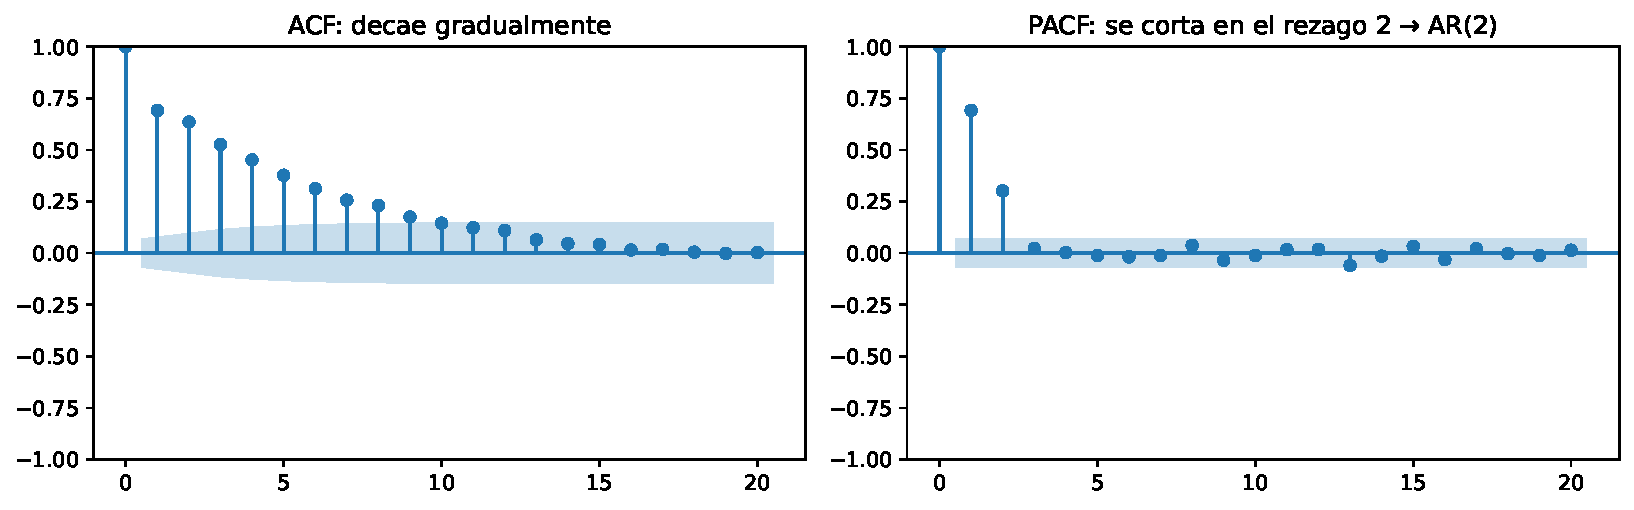
\includegraphics[keepaspectratio]{unidad3/cap16_series_temporales_macro_files/figure-pdf/acf-pacf-output-1.pdf}}

La PACF muestra dos barras significativas y luego nada: la firma de un
AR(2). En la práctica, la identificación visual se complementa con
criterios de información (AIC/BIC): ajustar varios órdenes candidatos y
quedarse con el que mejor balancea ajuste y parsimonia.

\begin{center}\rule{0.5\linewidth}{0.5pt}\end{center}

\chapter{ARIMA en acción: modelar y pronosticar la
inflación}\label{arima-en-acciuxf3n-modelar-y-pronosticar-la-inflaciuxf3n}

Armemos el flujo completo con una serie macro simulada con la
persistencia típica de la inflación mensual.

\phantomsection\label{arima-ajuste}
\begin{Shaded}
\begin{Highlighting}[]
\CommentTok{\# Serie mensual de "inflación" con inercia AR(1) fuerte (phi=0.75)}
\NormalTok{n }\OperatorTok{=} \DecValTok{240}   \CommentTok{\# 20 años}
\NormalTok{inflacion }\OperatorTok{=}\NormalTok{ np.zeros(n)}
\NormalTok{mu\_inf }\OperatorTok{=} \FloatTok{2.0} \OperatorTok{/} \DecValTok{12}  \CommentTok{\# \textasciitilde{}2\% anual en mensual}
\ControlFlowTok{for}\NormalTok{ t }\KeywordTok{in} \BuiltInTok{range}\NormalTok{(}\DecValTok{1}\NormalTok{, n):}
\NormalTok{    inflacion[t] }\OperatorTok{=}\NormalTok{ mu\_inf }\OperatorTok{*} \FloatTok{0.25} \OperatorTok{+} \FloatTok{0.75} \OperatorTok{*}\NormalTok{ inflacion[t}\OperatorTok{{-}}\DecValTok{1}\NormalTok{] }\OperatorTok{+}\NormalTok{ rng.normal(}\DecValTok{0}\NormalTok{, }\FloatTok{0.15}\NormalTok{)}

\NormalTok{fechas }\OperatorTok{=}\NormalTok{ pd.date\_range(}\StringTok{"2006{-}01{-}01"}\NormalTok{, periods}\OperatorTok{=}\NormalTok{n, freq}\OperatorTok{=}\StringTok{"MS"}\NormalTok{)}
\NormalTok{serie }\OperatorTok{=}\NormalTok{ pd.Series(inflacion, index}\OperatorTok{=}\NormalTok{fechas, name}\OperatorTok{=}\StringTok{"inflacion\_mensual"}\NormalTok{)}

\CommentTok{\# 1) ¿Estacionaria?}
\NormalTok{stat, pval }\OperatorTok{=}\NormalTok{ adfuller(serie)[:}\DecValTok{2}\NormalTok{]}
\BuiltInTok{print}\NormalTok{(}\SpecialStringTok{f"ADF: stat=}\SpecialCharTok{\{}\NormalTok{stat}\SpecialCharTok{:.2f\}}\SpecialStringTok{, p{-}value=}\SpecialCharTok{\{}\NormalTok{pval}\SpecialCharTok{:.4f\}}\SpecialStringTok{ → "}
      \SpecialStringTok{f"}\SpecialCharTok{\{}\StringTok{\textquotesingle{}estacionaria, no hace falta diferenciar (d=0)\textquotesingle{}} \ControlFlowTok{if}\NormalTok{ pval }\OperatorTok{\textless{}} \FloatTok{0.05} \ControlFlowTok{else} \StringTok{\textquotesingle{}diferenciar\textquotesingle{}}\SpecialCharTok{\}}\SpecialStringTok{"}\NormalTok{)}

\CommentTok{\# 2) Selección de orden por AIC entre algunos candidatos}
\NormalTok{candidatos }\OperatorTok{=}\NormalTok{ [(}\DecValTok{1}\NormalTok{,}\DecValTok{0}\NormalTok{,}\DecValTok{0}\NormalTok{), (}\DecValTok{2}\NormalTok{,}\DecValTok{0}\NormalTok{,}\DecValTok{0}\NormalTok{), (}\DecValTok{1}\NormalTok{,}\DecValTok{0}\NormalTok{,}\DecValTok{1}\NormalTok{), (}\DecValTok{0}\NormalTok{,}\DecValTok{0}\NormalTok{,}\DecValTok{2}\NormalTok{)]}
\NormalTok{aics }\OperatorTok{=}\NormalTok{ \{orden: ARIMA(serie, order}\OperatorTok{=}\NormalTok{orden).fit().aic }\ControlFlowTok{for}\NormalTok{ orden }\KeywordTok{in}\NormalTok{ candidatos\}}
\NormalTok{mejor }\OperatorTok{=} \BuiltInTok{min}\NormalTok{(aics, key}\OperatorTok{=}\NormalTok{aics.get)}
\BuiltInTok{print}\NormalTok{(}\StringTok{"}\CharTok{\textbackslash{}n}\StringTok{AIC por modelo candidato:"}\NormalTok{)}
\ControlFlowTok{for}\NormalTok{ orden, aic }\KeywordTok{in}\NormalTok{ aics.items():}
\NormalTok{    marca }\OperatorTok{=} \StringTok{"  ← elegido"} \ControlFlowTok{if}\NormalTok{ orden }\OperatorTok{==}\NormalTok{ mejor }\ControlFlowTok{else} \StringTok{""}
    \BuiltInTok{print}\NormalTok{(}\SpecialStringTok{f"  ARIMA}\SpecialCharTok{\{}\NormalTok{orden}\SpecialCharTok{\}}\SpecialStringTok{: }\SpecialCharTok{\{}\NormalTok{aic}\SpecialCharTok{:8.1f\}\{}\NormalTok{marca}\SpecialCharTok{\}}\SpecialStringTok{"}\NormalTok{)}

\CommentTok{\# 3) Ajuste final}
\NormalTok{modelo }\OperatorTok{=}\NormalTok{ ARIMA(serie, order}\OperatorTok{=}\NormalTok{mejor).fit()}
\BuiltInTok{print}\NormalTok{(}\SpecialStringTok{f"}\CharTok{\textbackslash{}n}\SpecialStringTok{Coeficientes del ARIMA}\SpecialCharTok{\{}\NormalTok{mejor}\SpecialCharTok{\}}\SpecialStringTok{:"}\NormalTok{)}
\BuiltInTok{print}\NormalTok{(modelo.params.}\BuiltInTok{round}\NormalTok{(}\DecValTok{3}\NormalTok{))}
\end{Highlighting}
\end{Shaded}

\begin{verbatim}
ADF: stat=-5.25, p-value=0.0000 → estacionaria, no hace falta diferenciar (d=0)

AIC por modelo candidato:
  ARIMA(1, 0, 0):   -236.9
  ARIMA(2, 0, 0):   -237.8
  ARIMA(1, 0, 1):   -238.1  ← elegido
  ARIMA(0, 0, 2):   -196.3

Coeficientes del ARIMA(1, 0, 1):
const     0.165
ar.L1     0.762
ma.L1     0.145
sigma2    0.021
dtype: float64
\end{verbatim}

El AIC elige el AR(1) ---el proceso generador verdadero--- y el
coeficiente estimado ronda el 0.75 real. Ahora, el pronóstico:

\begin{Shaded}
\begin{Highlighting}[]
\NormalTok{horizonte }\OperatorTok{=} \DecValTok{24}
\NormalTok{pron }\OperatorTok{=}\NormalTok{ modelo.get\_forecast(steps}\OperatorTok{=}\NormalTok{horizonte)}
\NormalTok{media }\OperatorTok{=}\NormalTok{ pron.predicted\_mean}
\NormalTok{banda }\OperatorTok{=}\NormalTok{ pron.conf\_int(alpha}\OperatorTok{=}\FloatTok{0.05}\NormalTok{)}

\NormalTok{fig, ax }\OperatorTok{=}\NormalTok{ plt.subplots(figsize}\OperatorTok{=}\NormalTok{(}\DecValTok{10}\NormalTok{, }\FloatTok{4.5}\NormalTok{))}
\NormalTok{ax.plot(serie.iloc[}\OperatorTok{{-}}\DecValTok{72}\NormalTok{:], label}\OperatorTok{=}\StringTok{"Inflación observada"}\NormalTok{)}
\NormalTok{ax.plot(media, }\StringTok{"r{-}"}\NormalTok{, linewidth}\OperatorTok{=}\DecValTok{2}\NormalTok{, label}\OperatorTok{=}\StringTok{"Pronóstico ARIMA"}\NormalTok{)}
\NormalTok{ax.fill\_between(banda.index, banda.iloc[:, }\DecValTok{0}\NormalTok{], banda.iloc[:, }\DecValTok{1}\NormalTok{],}
\NormalTok{                alpha}\OperatorTok{=}\FloatTok{0.2}\NormalTok{, color}\OperatorTok{=}\StringTok{"red"}\NormalTok{, label}\OperatorTok{=}\StringTok{"IC 95\%"}\NormalTok{)}
\NormalTok{ax.set\_ylabel(}\StringTok{"Inflación mensual (\%)"}\NormalTok{)}
\NormalTok{ax.set\_title(}\StringTok{"Pronóstico a 24 meses con intervalos de confianza"}\NormalTok{)}
\NormalTok{ax.legend()}
\NormalTok{ax.grid(}\VariableTok{True}\NormalTok{, alpha}\OperatorTok{=}\FloatTok{0.3}\NormalTok{)}
\NormalTok{plt.tight\_layout()}
\NormalTok{plt.show()}
\end{Highlighting}
\end{Shaded}

\pandocbounded{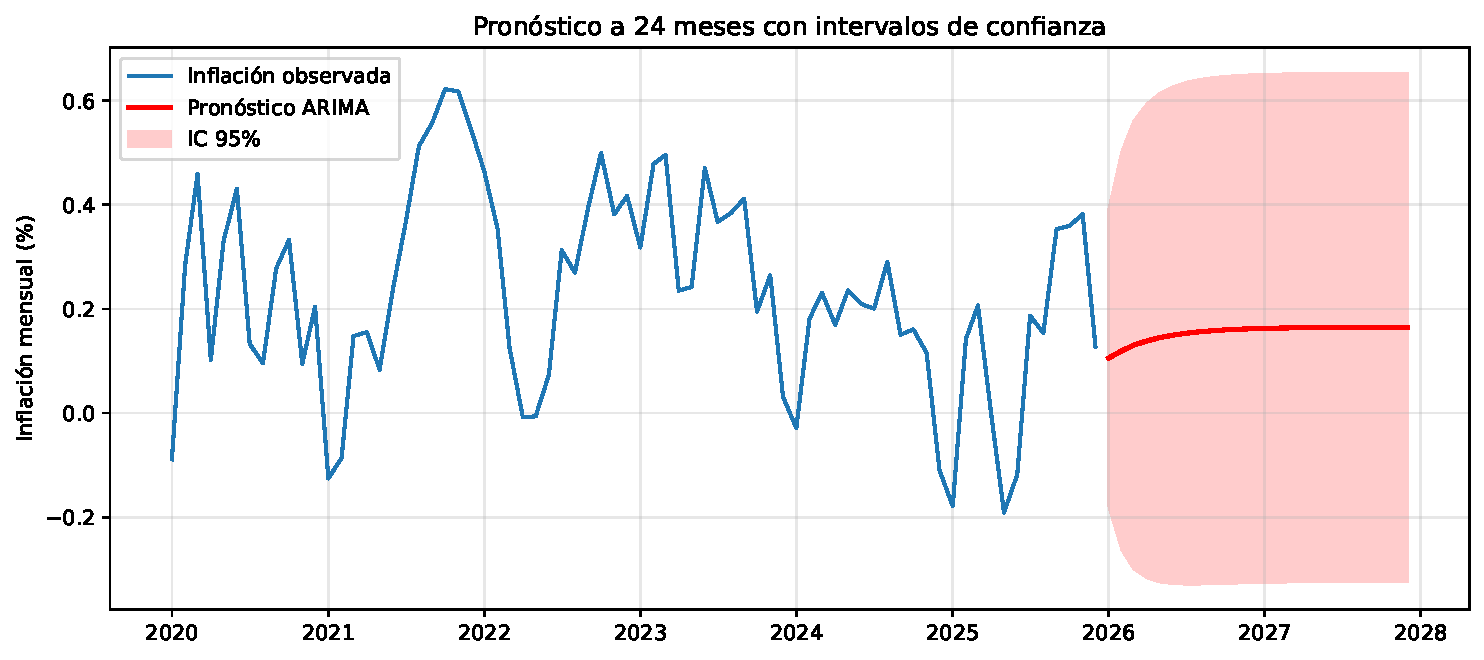
\includegraphics[keepaspectratio]{unidad3/cap16_series_temporales_macro_files/figure-pdf/arima-pronostico-output-1.pdf}}

Dos rasgos para leer en el gráfico, típicos de todo pronóstico ARIMA: la
predicción \textbf{converge a la media de largo plazo} de la serie (la
inercia se agota), y las bandas \textbf{se abren con el horizonte} hasta
estabilizarse --- el modelo es honesto sobre lo poco que sabe del futuro
lejano.

\begin{tcolorbox}[enhanced jigsaw, bottomrule=.15mm, colback=white, opacitybacktitle=0.6, arc=.35mm, toprule=.15mm, opacityback=0, breakable, titlerule=0mm, left=2mm, coltitle=black, colbacktitle=quarto-callout-warning-color!10!white, colframe=quarto-callout-warning-color-frame, leftrule=.75mm, toptitle=1mm, bottomtitle=1mm, title=\textcolor{quarto-callout-warning-color}{\faExclamationTriangle}\hspace{0.5em}{¿Y pronosticar retornos de acciones?}, rightrule=.15mm]

Tentador, pero el ARIMA sobre retornos accionarios suele
encontrar\ldots{} nada (\(p = q = 0\)): los retornos son casi
impredecibles por su propio pasado (eficiencia de mercado en su forma
débil). Donde los modelos de series de tiempo brillan es en variables
\textbf{con inercia estructural}: inflación, tasas, actividad, y ---muy
especialmente--- la \emph{volatilidad} (la familia GARCH, prima hermana
de ARMA aplicada a la varianza).

\end{tcolorbox}

\begin{center}\rule{0.5\linewidth}{0.5pt}\end{center}

\chapter{VAR: varias series que se influyen
mutuamente}\label{var-varias-series-que-se-influyen-mutuamente}

La macro rara vez es univariada: la inflación depende de la tasa de
interés, la tasa responde a la inflación, y la actividad interactúa con
ambas. El modelo \textbf{VAR} (\emph{Vector Autoregression}) generaliza
el AR a un \textbf{sistema}: cada variable se regresa sobre los rezagos
de \textbf{todas} las variables.

Para dos variables y un rezago:

\[\begin{aligned} y_{1,t} &= c_1 + \phi_{11}\, y_{1,t-1} + \phi_{12}\, y_{2,t-1} + \varepsilon_{1,t} \\ y_{2,t} &= c_2 + \phi_{21}\, y_{1,t-1} + \phi_{22}\, y_{2,t-1} + \varepsilon_{2,t} \end{aligned}\]

Los coeficientes cruzados (\(\phi_{12}, \phi_{21}\)) son la novedad:
capturan cómo una variable \textbf{anticipa} a la otra.

\phantomsection\label{var-datos}
\begin{Shaded}
\begin{Highlighting}[]
\CommentTok{\# Sistema simulado con estructura conocida:}
\CommentTok{\#   {-} la tasa sube cuando la inflación pasada fue alta (regla de política)}
\CommentTok{\#   {-} la inflación baja cuando la tasa pasada fue alta (efecto de la política)}
\NormalTok{n }\OperatorTok{=} \DecValTok{300}
\NormalTok{inf }\OperatorTok{=}\NormalTok{ np.zeros(n)}
\NormalTok{tasa }\OperatorTok{=}\NormalTok{ np.zeros(n)}
\ControlFlowTok{for}\NormalTok{ t }\KeywordTok{in} \BuiltInTok{range}\NormalTok{(}\DecValTok{1}\NormalTok{, n):}
\NormalTok{    inf[t] }\OperatorTok{=} \FloatTok{0.6} \OperatorTok{*}\NormalTok{ inf[t}\OperatorTok{{-}}\DecValTok{1}\NormalTok{] }\OperatorTok{{-}} \FloatTok{0.20} \OperatorTok{*}\NormalTok{ tasa[t}\OperatorTok{{-}}\DecValTok{1}\NormalTok{] }\OperatorTok{+}\NormalTok{ rng.normal(}\DecValTok{0}\NormalTok{, }\FloatTok{0.3}\NormalTok{)}
\NormalTok{    tasa[t] }\OperatorTok{=} \FloatTok{0.7} \OperatorTok{*}\NormalTok{ tasa[t}\OperatorTok{{-}}\DecValTok{1}\NormalTok{] }\OperatorTok{+} \FloatTok{0.25} \OperatorTok{*}\NormalTok{ inf[t}\OperatorTok{{-}}\DecValTok{1}\NormalTok{] }\OperatorTok{+}\NormalTok{ rng.normal(}\DecValTok{0}\NormalTok{, }\FloatTok{0.2}\NormalTok{)}

\NormalTok{datos }\OperatorTok{=}\NormalTok{ pd.DataFrame(\{}\StringTok{"inflacion"}\NormalTok{: inf, }\StringTok{"tasa"}\NormalTok{: tasa\},}
\NormalTok{                     index}\OperatorTok{=}\NormalTok{pd.date\_range(}\StringTok{"2001{-}01{-}01"}\NormalTok{, periods}\OperatorTok{=}\NormalTok{n, freq}\OperatorTok{=}\StringTok{"MS"}\NormalTok{))}

\CommentTok{\# Ajuste del VAR con selección automática del número de rezagos}
\NormalTok{var\_modelo }\OperatorTok{=}\NormalTok{ VAR(datos)}
\NormalTok{seleccion }\OperatorTok{=}\NormalTok{ var\_modelo.select\_order(maxlags}\OperatorTok{=}\DecValTok{8}\NormalTok{)}
\NormalTok{p\_optimo }\OperatorTok{=}\NormalTok{ seleccion.aic}
\NormalTok{resultado }\OperatorTok{=}\NormalTok{ var\_modelo.fit(p\_optimo)}

\BuiltInTok{print}\NormalTok{(}\SpecialStringTok{f"Rezagos elegidos por AIC: }\SpecialCharTok{\{}\NormalTok{p\_optimo}\SpecialCharTok{\}}\CharTok{\textbackslash{}n}\SpecialStringTok{"}\NormalTok{)}
\BuiltInTok{print}\NormalTok{(}\StringTok{"Coeficientes de la ecuación de inflación:"}\NormalTok{)}
\BuiltInTok{print}\NormalTok{(resultado.params[}\StringTok{"inflacion"}\NormalTok{].}\BuiltInTok{round}\NormalTok{(}\DecValTok{3}\NormalTok{))}
\end{Highlighting}
\end{Shaded}

\begin{verbatim}
Rezagos elegidos por AIC: 1

Coeficientes de la ecuación de inflación:
const          -0.018
L1.inflacion    0.611
L1.tasa        -0.156
Name: inflacion, dtype: float64
\end{verbatim}

Los coeficientes recuperan la estructura que sembramos: la inflación
depende positivamente de su pasado y \textbf{negativamente de la tasa
pasada}. Pero la forma más útil de leer un VAR no es la tabla de
coeficientes sino la\ldots{}

\section{Función de impulso-respuesta
(IRF)}\label{funciuxf3n-de-impulso-respuesta-irf}

La IRF responde la pregunta de política: \emph{si hoy golpeo al sistema
con un shock de una unidad en una variable, ¿cómo evolucionan todas las
variables en los meses siguientes?} Es el experimento contrafáctico que
el VAR permite trazar.

\begin{Shaded}
\begin{Highlighting}[]
\NormalTok{irf }\OperatorTok{=}\NormalTok{ resultado.irf(}\DecValTok{24}\NormalTok{)}
\NormalTok{irf.plot(orth}\OperatorTok{=}\VariableTok{False}\NormalTok{, figsize}\OperatorTok{=}\NormalTok{(}\DecValTok{10}\NormalTok{, }\DecValTok{7}\NormalTok{))}
\NormalTok{plt.suptitle(}\StringTok{"Funciones de impulso{-}respuesta (24 meses)"}\NormalTok{, y}\OperatorTok{=}\FloatTok{1.02}\NormalTok{)}
\NormalTok{plt.tight\_layout()}
\NormalTok{plt.show()}
\end{Highlighting}
\end{Shaded}

\pandocbounded{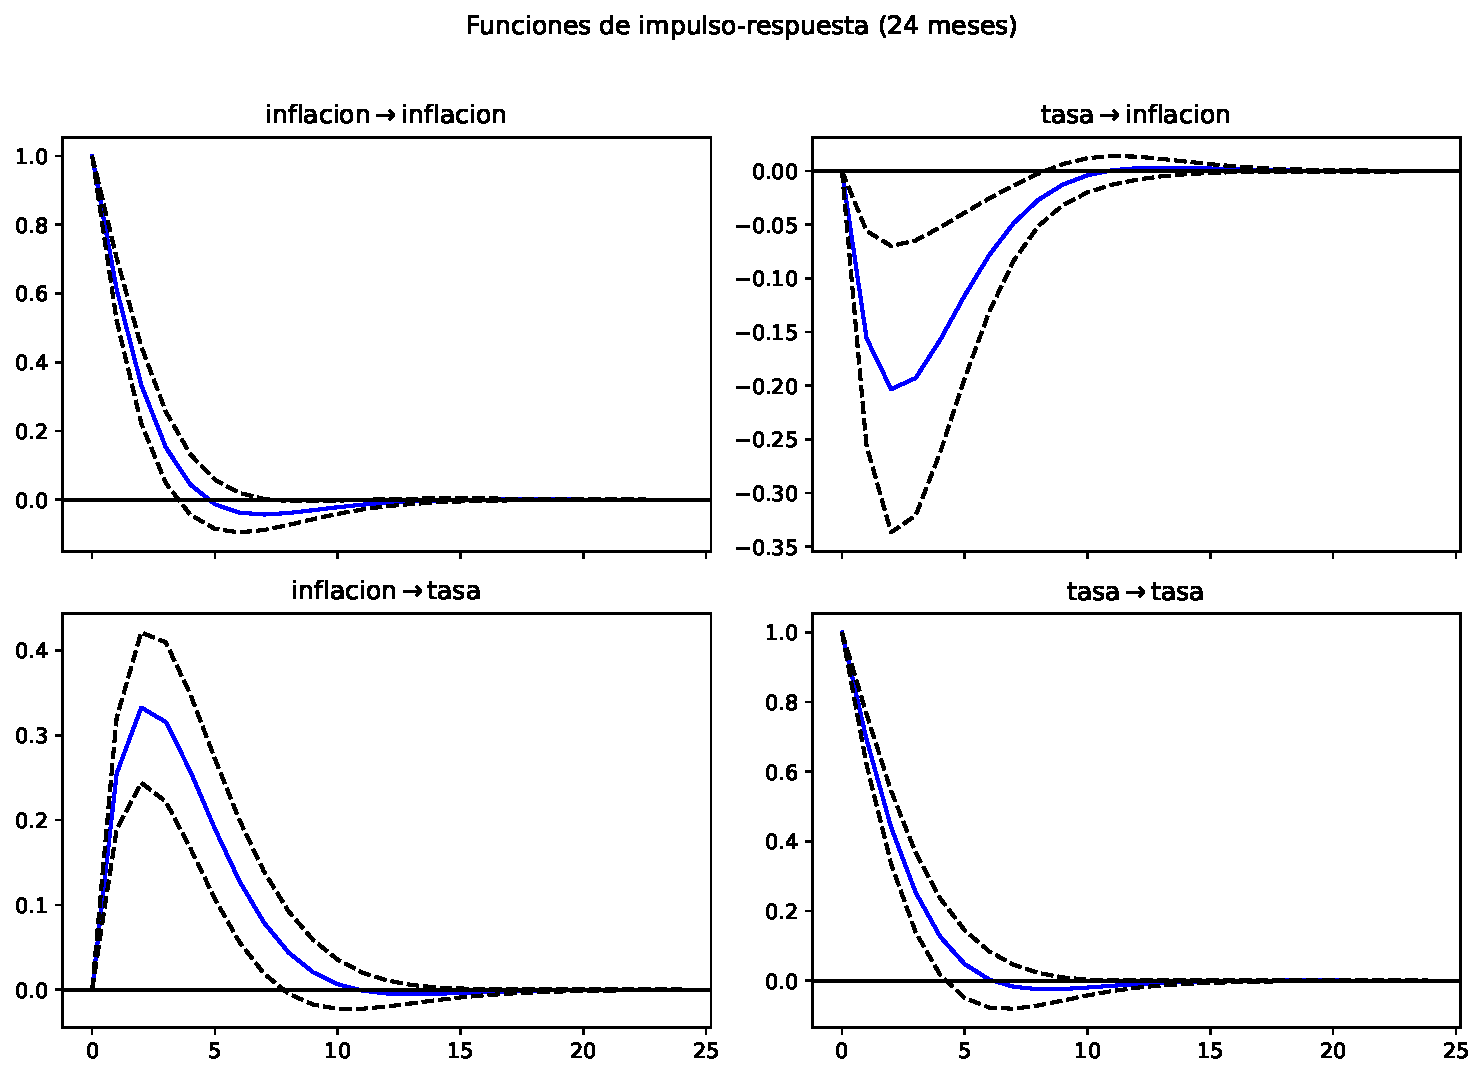
\includegraphics[keepaspectratio]{unidad3/cap16_series_temporales_macro_files/figure-pdf/var-irf-output-1.pdf}}

Mirá el panel ``tasa → inflacion'': un shock de tasa deprime la
inflación durante varios meses, con el efecto máximo no inmediato sino
rezagado --- exactamente la dinámica ``la política monetaria actúa con
rezagos'' que los bancos centrales repiten. El panel ``inflacion →
tasa'' muestra la respuesta de política: la tasa sube tras un shock
inflacionario y luego decae.

\begin{tcolorbox}[enhanced jigsaw, bottomrule=.15mm, colback=white, opacitybacktitle=0.6, arc=.35mm, toprule=.15mm, opacityback=0, breakable, titlerule=0mm, left=2mm, coltitle=black, colbacktitle=quarto-callout-note-color!10!white, colframe=quarto-callout-note-color-frame, leftrule=.75mm, toptitle=1mm, bottomtitle=1mm, title=\textcolor{quarto-callout-note-color}{\faInfo}\hspace{0.5em}{Los VAR en la práctica}, rightrule=.15mm]

Los bancos centrales usan VARs (y variantes: SVAR, BVAR, FAVAR) como
caballo de batalla para el análisis de política monetaria desde los
trabajos de Sims (Nobel 2011). En finanzas se usan para sistemas
tasa-inflación-actividad, para pronóstico macro que alimenta modelos de
PPNR y stress testing (Capítulo 12), y para estudiar transmisión entre
mercados.

\end{tcolorbox}

\begin{center}\rule{0.5\linewidth}{0.5pt}\end{center}

\chapter{Errores comunes}\label{errores-comunes-14}

\begin{tcolorbox}[enhanced jigsaw, bottomrule=.15mm, colback=white, opacitybacktitle=0.6, arc=.35mm, toprule=.15mm, opacityback=0, breakable, titlerule=0mm, left=2mm, coltitle=black, colbacktitle=quarto-callout-warning-color!10!white, colframe=quarto-callout-warning-color-frame, leftrule=.75mm, toptitle=1mm, bottomtitle=1mm, title=\textcolor{quarto-callout-warning-color}{\faExclamationTriangle}\hspace{0.5em}{Trampas frecuentes}, rightrule=.15mm]

\begin{itemize}
\tightlist
\item
  \textbf{Modelar en niveles sin testear estacionariedad}: la regresión
  espuria del inicio. ADF primero, modelo después.
\item
  \textbf{Sobrediferenciar}: si la serie ya era estacionaria,
  diferenciarla ``por las dudas'' introduce un MA espurio y arruina el
  pronóstico. La ``d'' correcta es la mínima necesaria.
\item
  \textbf{Elegir p y q maximizando el ajuste dentro de la muestra}: más
  rezagos siempre ajustan mejor \emph{in-sample}; usá AIC/BIC o
  validación fuera de muestra (el tema del próximo capítulo).
\item
  \textbf{Leer causalidad en un VAR}: que la tasa ``anticipe'' a la
  inflación (precedencia temporal, causalidad de Granger) no prueba
  causalidad económica; puede haber una tercera variable moviendo a
  ambas.
\item
  \textbf{Ignorar los residuos}: un buen modelo deja residuos sin
  autocorrelación. Si la ACF de los residuos muestra estructura, el
  modelo se quedó corto.
\end{itemize}

\end{tcolorbox}

\begin{center}\rule{0.5\linewidth}{0.5pt}\end{center}

\chapter{Ejercicios Propuestos}\label{ejercicios-propuestos-15}

\begin{tcolorbox}[enhanced jigsaw, bottomrule=.15mm, colback=white, opacitybacktitle=0.6, arc=.35mm, toprule=.15mm, opacityback=0, breakable, titlerule=0mm, left=2mm, coltitle=black, colbacktitle=quarto-callout-important-color!10!white, colframe=quarto-callout-important-color-frame, leftrule=.75mm, toptitle=1mm, bottomtitle=1mm, title=\textcolor{quarto-callout-important-color}{\faExclamation}\hspace{0.5em}{Ejercicios}, rightrule=.15mm]

\begin{enumerate}
\def\labelenumi{\arabic{enumi}.}
\tightlist
\item
  \textbf{Identificación}: generá un MA(2) puro y verificá con ACF/PACF
  que la firma es la esperada (ACF cortada en 2, PACF decayendo).
\item
  \textbf{d correcta}: tomá la serie de ``precios'' acumulando los
  retornos del capítulo, ajustale un ARIMA(1,1,0) y compará con ajustar
  ARIMA(1,0,0) a los retornos. ¿Son el mismo modelo?
\item
  \textbf{Backtest de pronóstico}: dividí la serie de inflación en 80\%
  entrenamiento / 20\% prueba, pronosticá el tramo final y calculá el
  error cuadrático medio contra un pronóstico ingenuo (``mañana =
  hoy''). ¿El ARIMA le gana?
\item
  \textbf{Causalidad de Granger}: usá \texttt{resultado.test\_causality}
  para testear si la tasa ``Granger-causa'' a la inflación en el VAR del
  capítulo, y viceversa.
\item
  \textbf{VAR de tres variables}: agregá al sistema una variable de
  ``actividad'' que dependa negativamente de la tasa, re-estimá el VAR y
  analizá las nuevas IRF.
\end{enumerate}

\end{tcolorbox}

Podés resolver estos ejercicios acá mismo: la celda ejecuta Python
\textbf{en tu navegador}, sin instalar nada (la primera ejecución tarda
unos segundos mientras carga el entorno; los paquetes que importes se
instalan solos).

\begin{Shaded}
\begin{Highlighting}[]
\NormalTok{\#| label: practica{-}navegador}
\NormalTok{import numpy as np}
\NormalTok{import statsmodels.api as sm}
\NormalTok{from statsmodels.tsa.arima.model import ARIMA}

\NormalTok{\# Tu solución acá...}
\end{Highlighting}
\end{Shaded}

\begin{center}\rule{0.5\linewidth}{0.5pt}\end{center}

\chapter{Referencias}\label{referencias-15}

\phantomsection\label{refs}

\chapter{Capítulo 17: Backtesting de
Estrategias}\label{capuxedtulo-17-backtesting-de-estrategias}

In-sample, out-of-sample, p-values y walk-forward

Cualquier estrategia parece brillante evaluada sobre los datos con los
que fue diseñada. Este capítulo construye la disciplina para saber si
funciona de verdad: separación in-sample / out-of-sample, el peligro del
sobreajuste y del data snooping, cómo calcular e interpretar el p-value
de una estrategia, el análisis walk-forward como estándar profesional, y
las métricas correctas para juzgar el desempeño fuera de muestra.

\hfill\break

\chapter{Introducción}\label{introducciuxf3n-14}

Cerramos el módulo con la pregunta que une todo lo anterior: tenés una
estrategia ---una regla que decide cuándo comprar y vender--- y su
simulación histórica da ganancias. \textbf{¿Eso prueba algo?}

Casi siempre, no. El problema es estructural: la estrategia se diseñó
\emph{mirando} esos mismos datos. Ajustaste parámetros, probaste
variantes, descartaste lo que no andaba\ldots{} y lo que sobrevivió,
sobrevivió \emph{por construcción}. Es como rendir un examen habiendo
visto las respuestas: la nota no mide conocimiento.

El \textbf{backtesting} riguroso es el conjunto de prácticas para
separar la señal de la casualidad. Es, en el fondo, el método científico
aplicado al trading: hipótesis primero, evidencia después, y una
paranoia saludable hacia los resultados demasiado lindos.

\phantomsection\label{setup}
\begin{Shaded}
\begin{Highlighting}[]
\ImportTok{import}\NormalTok{ numpy }\ImportTok{as}\NormalTok{ np}
\ImportTok{import}\NormalTok{ pandas }\ImportTok{as}\NormalTok{ pd}
\ImportTok{import}\NormalTok{ matplotlib.pyplot }\ImportTok{as}\NormalTok{ plt}
\ImportTok{from}\NormalTok{ scipy }\ImportTok{import}\NormalTok{ stats}

\NormalTok{rng }\OperatorTok{=}\NormalTok{ np.random.default\_rng(}\DecValTok{42}\NormalTok{)}
\end{Highlighting}
\end{Shaded}

\begin{center}\rule{0.5\linewidth}{0.5pt}\end{center}

\chapter{El pecado original: evaluar donde
diseñaste}\label{el-pecado-original-evaluar-donde-diseuxf1aste}

\section{In-sample vs.~out-of-sample}\label{in-sample-vs.-out-of-sample}

La división fundamental:

\begin{itemize}
\tightlist
\item
  \textbf{In-sample (IS)}: los datos usados para \emph{diseñar} la
  estrategia (elegir reglas, calibrar parámetros). Ahí la estrategia
  siempre luce bien --- la elegiste porque lucía bien ahí.
\item
  \textbf{Out-of-sample (OOS)}: datos que la estrategia \textbf{nunca
  vio}. La única evidencia admisible sobre su capacidad real.
\end{itemize}

La demostración más contundente de por qué esto importa: vamos a
``descubrir'' una estrategia excelente \textbf{en puro ruido}.

\phantomsection\label{data-snooping}
\begin{Shaded}
\begin{Highlighting}[]
\CommentTok{\# 10 años de retornos diarios SIN NINGUNA señal: puro azar con drift cero}
\NormalTok{n\_dias }\OperatorTok{=} \DecValTok{2520}
\NormalTok{retornos }\OperatorTok{=}\NormalTok{ rng.normal(}\FloatTok{0.0}\NormalTok{, }\FloatTok{0.012}\NormalTok{, n\_dias)}
\NormalTok{train, test }\OperatorTok{=}\NormalTok{ retornos[:}\DecValTok{1680}\NormalTok{], retornos[}\DecValTok{1680}\NormalTok{:]   }\CommentTok{\# \textasciitilde{}2/3 diseño, 1/3 evaluación}

\KeywordTok{def}\NormalTok{ estrategia\_momentum(r, ventana):}
    \CommentTok{"""Compra si la media de los últimos \textasciigrave{}ventana\textasciigrave{} días fue positiva."""}
\NormalTok{    señal }\OperatorTok{=}\NormalTok{ np.array([r[}\BuiltInTok{max}\NormalTok{(}\DecValTok{0}\NormalTok{, t}\OperatorTok{{-}}\NormalTok{ventana):t].mean() }\OperatorTok{\textgreater{}} \DecValTok{0} \ControlFlowTok{for}\NormalTok{ t }\KeywordTok{in} \BuiltInTok{range}\NormalTok{(}\BuiltInTok{len}\NormalTok{(r))])}
    \ControlFlowTok{return}\NormalTok{ np.where(señal, r, }\FloatTok{0.0}\NormalTok{)   }\CommentTok{\# invertido o en cash}

\KeywordTok{def}\NormalTok{ sharpe(r):}
    \ControlFlowTok{return}\NormalTok{ r.mean() }\OperatorTok{/}\NormalTok{ r.std() }\OperatorTok{*}\NormalTok{ np.sqrt(}\DecValTok{252}\NormalTok{) }\ControlFlowTok{if}\NormalTok{ r.std() }\OperatorTok{\textgreater{}} \DecValTok{0} \ControlFlowTok{else} \FloatTok{0.0}

\CommentTok{\# "Investigación": probamos 60 ventanas distintas y elegimos la mejor IN{-}SAMPLE}
\NormalTok{ventanas }\OperatorTok{=} \BuiltInTok{range}\NormalTok{(}\DecValTok{2}\NormalTok{, }\DecValTok{62}\NormalTok{)}
\NormalTok{sharpes\_is }\OperatorTok{=}\NormalTok{ \{v: sharpe(estrategia\_momentum(train, v)) }\ControlFlowTok{for}\NormalTok{ v }\KeywordTok{in}\NormalTok{ ventanas\}}
\NormalTok{mejor\_v }\OperatorTok{=} \BuiltInTok{max}\NormalTok{(sharpes\_is, key}\OperatorTok{=}\NormalTok{sharpes\_is.get)}

\BuiltInTok{print}\NormalTok{(}\SpecialStringTok{f"Ventanas probadas: }\SpecialCharTok{\{}\BuiltInTok{len}\NormalTok{(}\BuiltInTok{list}\NormalTok{(ventanas))}\SpecialCharTok{\}}\SpecialStringTok{"}\NormalTok{)}
\BuiltInTok{print}\NormalTok{(}\SpecialStringTok{f"Mejor ventana in{-}sample: }\SpecialCharTok{\{}\NormalTok{mejor\_v}\SpecialCharTok{\}}\SpecialStringTok{ días → Sharpe IS = }\SpecialCharTok{\{}\NormalTok{sharpes\_is[mejor\_v]}\SpecialCharTok{:.2f\}}\SpecialStringTok{"}\NormalTok{)}
\BuiltInTok{print}\NormalTok{(}\SpecialStringTok{f"La misma estrategia out{-}of{-}sample:   Sharpe OOS = "}
      \SpecialStringTok{f"}\SpecialCharTok{\{}\NormalTok{sharpe(estrategia\_momentum(test, mejor\_v))}\SpecialCharTok{:.2f\}}\SpecialStringTok{"}\NormalTok{)}
\end{Highlighting}
\end{Shaded}

\begin{verbatim}
Ventanas probadas: 60
Mejor ventana in-sample: 7 días → Sharpe IS = -0.06
La misma estrategia out-of-sample:   Sharpe OOS = 0.16
\end{verbatim}

Los datos son \textbf{ruido puro por construcción} --- no hay nada que
descubrir. Y sin embargo, probando 60 variantes, alguna siempre luce
bien in-sample. Fuera de muestra, el castillo se derrumba. Ese mecanismo
tiene nombre: \textbf{data snooping} (o \emph{p-hacking}): probar hasta
que algo ``funcione'' garantiza encontrar espejismos.

\begin{tcolorbox}[enhanced jigsaw, bottomrule=.15mm, colback=white, opacitybacktitle=0.6, arc=.35mm, toprule=.15mm, opacityback=0, breakable, titlerule=0mm, left=2mm, coltitle=black, colbacktitle=quarto-callout-warning-color!10!white, colframe=quarto-callout-warning-color-frame, leftrule=.75mm, toptitle=1mm, bottomtitle=1mm, title=\textcolor{quarto-callout-warning-color}{\faExclamationTriangle}\hspace{0.5em}{La regla de oro}, rightrule=.15mm]

Los datos out-of-sample se usan \textbf{una sola vez}. Si evaluás en
OOS, no te gusta el resultado, retocás la estrategia y volvés a evaluar
en el mismo OOS\ldots{} el OOS acaba de convertirse en in-sample. Esta
regla es incómoda y por eso casi nadie la cumple --- y por eso la
mayoría de los backtests publicados no se replican.

\end{tcolorbox}

\section{Sobreajuste: la curva que
memoriza}\label{sobreajuste-la-curva-que-memoriza}

El data snooping es la versión ``entre estrategias'' de un fenómeno
general: el \textbf{sobreajuste} (\emph{overfitting}). Un modelo con
suficientes parámetros puede memorizar cualquier historia --- incluyendo
su ruido. Cuantos más parámetros libres tenga tu estrategia (ventanas,
umbrales, filtros, horarios), más capacidad tiene de ajustarse a
accidentes del pasado que no se repetirán.

Regla mental de López de Prado: \textbf{la probabilidad de que un
backtest sea falso crece con el número de configuraciones probadas} ---
y quien lo publica rara vez te dice cuántas probó.

\begin{center}\rule{0.5\linewidth}{0.5pt}\end{center}

\chapter{El p-value de una
estrategia}\label{el-p-value-de-una-estrategia}

¿Cómo cuantificar si un resultado OOS es ``suerte o señal''? Con la
misma lógica inferencial del Capítulo 15. La hipótesis nula es dura pero
justa:

\begin{quote}
\(H_0\): la estrategia no tiene ninguna habilidad (retorno medio
verdadero = 0).
\end{quote}

Bajo \(H_0\), el estadístico t del retorno medio nos dice cuán
sorprendente es lo observado:

\[t = \frac{\bar{r}}{s / \sqrt{n}} \qquad\text{y de hecho}\qquad t \approx \text{Sharpe anualizado} \times \sqrt{\text{años}}\]

Esa equivalencia es una de las fórmulas más útiles del oficio:
\textbf{el t-stat de una estrategia es su Sharpe por la raíz de los años
observados}. Un Sharpe de 1.0 necesita \textasciitilde4 años para ser
significativo al 5\%; un Sharpe de 0.5, ¡16 años!

\phantomsection\label{pvalue-estrategia}
\begin{Shaded}
\begin{Highlighting}[]
\KeywordTok{def}\NormalTok{ evaluar(r, nombre):}
\NormalTok{    n }\OperatorTok{=} \BuiltInTok{len}\NormalTok{(r)}
\NormalTok{    t\_stat }\OperatorTok{=}\NormalTok{ r.mean() }\OperatorTok{/}\NormalTok{ (r.std(ddof}\OperatorTok{=}\DecValTok{1}\NormalTok{) }\OperatorTok{/}\NormalTok{ np.sqrt(n))}
\NormalTok{    p\_value }\OperatorTok{=} \DecValTok{2} \OperatorTok{*}\NormalTok{ (}\DecValTok{1} \OperatorTok{{-}}\NormalTok{ stats.t.cdf(}\BuiltInTok{abs}\NormalTok{(t\_stat), df}\OperatorTok{=}\NormalTok{n }\OperatorTok{{-}} \DecValTok{1}\NormalTok{))}
    \BuiltInTok{print}\NormalTok{(}\SpecialStringTok{f"}\SpecialCharTok{\{}\NormalTok{nombre}\SpecialCharTok{:\textless{}28\}}\SpecialStringTok{ Sharpe: }\SpecialCharTok{\{}\NormalTok{sharpe(r)}\SpecialCharTok{:5.2f\}}\SpecialStringTok{ | t: }\SpecialCharTok{\{}\NormalTok{t\_stat}\SpecialCharTok{:5.2f\}}\SpecialStringTok{ | "}
          \SpecialStringTok{f"p{-}value: }\SpecialCharTok{\{}\NormalTok{p\_value}\SpecialCharTok{:.3f\}}\SpecialStringTok{"}\NormalTok{)}

\CommentTok{\# La estrategia "descubierta" en ruido, evaluada honestamente en OOS}
\NormalTok{evaluar(estrategia\_momentum(test, mejor\_v), }\StringTok{"Momentum sobre ruido (OOS)"}\NormalTok{)}

\CommentTok{\# Una estrategia con señal genuina (le sembramos un edge real, pequeño)}
\NormalTok{señal\_real }\OperatorTok{=}\NormalTok{ rng.normal(}\FloatTok{0.0004}\NormalTok{, }\FloatTok{0.012}\NormalTok{, }\DecValTok{840}\NormalTok{)   }\CommentTok{\# drift positivo verdadero}
\NormalTok{evaluar(señal\_real, }\StringTok{"Estrategia con edge real"}\NormalTok{)}
\end{Highlighting}
\end{Shaded}

\begin{verbatim}
Momentum sobre ruido (OOS)   Sharpe:  0.16 | t:  0.28 | p-value: 0.777
Estrategia con edge real     Sharpe:  1.23 | t:  2.24 | p-value: 0.025
\end{verbatim}

\begin{tcolorbox}[enhanced jigsaw, bottomrule=.15mm, colback=white, opacitybacktitle=0.6, arc=.35mm, toprule=.15mm, opacityback=0, breakable, titlerule=0mm, left=2mm, coltitle=black, colbacktitle=quarto-callout-warning-color!10!white, colframe=quarto-callout-warning-color-frame, leftrule=.75mm, toptitle=1mm, bottomtitle=1mm, title=\textcolor{quarto-callout-warning-color}{\faExclamationTriangle}\hspace{0.5em}{El p-value con trampa múltiple}, rightrule=.15mm]

Cuidado: ese p-value asume que evaluaste \textbf{una} estrategia. Si
probaste 60, la probabilidad de que \emph{alguna} pase el umbral del 5\%
por puro azar es enorme (\(1 - 0.95^{60} \approx 95\%\)). Las
correcciones (Bonferroni: exigir \(\alpha/N\); o el \emph{Deflated
Sharpe Ratio} de López de Prado) suben la vara según cuántas
configuraciones miraste. La honestidad estadística empieza por
\textbf{contar tus intentos}.

\end{tcolorbox}

\begin{center}\rule{0.5\linewidth}{0.5pt}\end{center}

\chapter{Walk-forward: el estándar
profesional}\label{walk-forward-el-estuxe1ndar-profesional}

La partición simple IS/OOS tiene una debilidad: la evaluación depende de
\emph{un} corte particular. Además, las estrategias reales se recalibran
periódicamente. El \textbf{análisis walk-forward} resuelve ambas cosas
imitando la operatoria real:

\begin{enumerate}
\def\labelenumi{\arabic{enumi}.}
\tightlist
\item
  \textbf{Entrená} (elegí parámetros) con una ventana de datos.
\item
  \textbf{Operá} con esos parámetros el período siguiente (nunca visto).
\item
  \textbf{Rodá} la ventana hacia adelante y repetí.
\item
  Concatená todos los tramos operados: eso es tu track record
  \textbf{100\% out-of-sample}.
\end{enumerate}

\phantomsection\label{walk-forward}
\begin{Shaded}
\begin{Highlighting}[]
\KeywordTok{def}\NormalTok{ walk\_forward(retornos, n\_train, n\_test, ventanas):}
    \CommentTok{"""Reoptimiza la ventana de momentum en cada tramo y opera el siguiente."""}
\NormalTok{    oos, elecciones }\OperatorTok{=}\NormalTok{ [], []}
\NormalTok{    inicio }\OperatorTok{=} \DecValTok{0}
    \ControlFlowTok{while}\NormalTok{ inicio }\OperatorTok{+}\NormalTok{ n\_train }\OperatorTok{+}\NormalTok{ n\_test }\OperatorTok{\textless{}=} \BuiltInTok{len}\NormalTok{(retornos):}
\NormalTok{        tramo\_train }\OperatorTok{=}\NormalTok{ retornos[inicio : inicio }\OperatorTok{+}\NormalTok{ n\_train]}
\NormalTok{        tramo\_test }\OperatorTok{=}\NormalTok{ retornos[inicio }\OperatorTok{+}\NormalTok{ n\_train : inicio }\OperatorTok{+}\NormalTok{ n\_train }\OperatorTok{+}\NormalTok{ n\_test]}

        \CommentTok{\# Optimización SOLO dentro del tramo de entrenamiento}
\NormalTok{        v\_opt }\OperatorTok{=} \BuiltInTok{max}\NormalTok{(ventanas, key}\OperatorTok{=}\KeywordTok{lambda}\NormalTok{ v: sharpe(estrategia\_momentum(tramo\_train, v)))}
\NormalTok{        elecciones.append(v\_opt)}

        \CommentTok{\# Operamos el tramo siguiente con lo elegido}
\NormalTok{        oos.append(estrategia\_momentum(tramo\_test, v\_opt))}
\NormalTok{        inicio }\OperatorTok{+=}\NormalTok{ n\_test    }\CommentTok{\# la ventana rueda}

    \ControlFlowTok{return}\NormalTok{ np.concatenate(oos), elecciones}

\CommentTok{\# Sobre el ruido puro: el walk{-}forward no se deja engañar}
\NormalTok{oos\_ruido, elecciones }\OperatorTok{=}\NormalTok{ walk\_forward(retornos, n\_train}\OperatorTok{=}\DecValTok{504}\NormalTok{, n\_test}\OperatorTok{=}\DecValTok{126}\NormalTok{,}
\NormalTok{                                     ventanas}\OperatorTok{=}\BuiltInTok{range}\NormalTok{(}\DecValTok{2}\NormalTok{, }\DecValTok{62}\NormalTok{))}
\BuiltInTok{print}\NormalTok{(}\SpecialStringTok{f"Tramos operados: }\SpecialCharTok{\{}\BuiltInTok{len}\NormalTok{(elecciones)}\SpecialCharTok{\}}\SpecialStringTok{ | Ventanas elegidas: }\SpecialCharTok{\{}\NormalTok{elecciones}\SpecialCharTok{\}}\SpecialStringTok{"}\NormalTok{)}
\NormalTok{evaluar(oos\_ruido, }\StringTok{"Walk{-}forward sobre ruido"}\NormalTok{)}
\end{Highlighting}
\end{Shaded}

\begin{verbatim}
Tramos operados: 16 | Ventanas elegidas: [2, 48, 41, 11, 11, 11, 3, 3, 3, 5, 10, 48, 17, 50, 15, 15]
Walk-forward sobre ruido     Sharpe: -0.56 | t: -1.58 | p-value: 0.114
\end{verbatim}

Dos observaciones valiosas: las \textbf{ventanas elegidas saltan
erráticamente} de tramo en tramo --- señal inequívoca de que no hay
estructura real que estimar, solo ruido que cambia de disfraz. Y el
desempeño concatenado es mediocre, como debe ser. Un walk-forward con
parámetros \emph{estables} entre tramos y desempeño OOS consistente es
de las mejores señales de que una estrategia es genuina.

\begin{center}\rule{0.5\linewidth}{0.5pt}\end{center}

\chapter{Métricas para juzgar el track record
OOS}\label{muxe9tricas-para-juzgar-el-track-record-oos}

Con el track record fuera de muestra en la mano, ¿qué mirar? Ninguna
métrica sola alcanza; el tablero mínimo:

\begin{longtable}[]{@{}
  >{\raggedright\arraybackslash}p{(\linewidth - 4\tabcolsep) * \real{0.3333}}
  >{\raggedright\arraybackslash}p{(\linewidth - 4\tabcolsep) * \real{0.3333}}
  >{\raggedright\arraybackslash}p{(\linewidth - 4\tabcolsep) * \real{0.3333}}@{}}
\toprule\noalign{}
\begin{minipage}[b]{\linewidth}\raggedright
Métrica
\end{minipage} & \begin{minipage}[b]{\linewidth}\raggedright
Qué mide
\end{minipage} & \begin{minipage}[b]{\linewidth}\raggedright
Talón de Aquiles
\end{minipage} \\
\midrule\noalign{}
\endhead
\bottomrule\noalign{}
\endlastfoot
\textbf{Sharpe anualizado} & Retorno en exceso por unidad de riesgo &
Ciego a la asimetría y a las rachas \\
\textbf{Máximo drawdown} & La peor caída pico-a-valle & Una sola
observación; muy sensible al período \\
\textbf{Hit ratio} & \% de períodos ganadores & Ignora tamaños: podés
acertar 60\% y quebrar \\
\textbf{Profit factor} & Ganancias brutas / pérdidas brutas & Inestable
con pocas operaciones \\
\end{longtable}

\phantomsection\label{metricas}
\begin{Shaded}
\begin{Highlighting}[]
\KeywordTok{def}\NormalTok{ reporte(r, nombre):}
\NormalTok{    equity }\OperatorTok{=}\NormalTok{ np.cumprod(}\DecValTok{1} \OperatorTok{+}\NormalTok{ r)}
\NormalTok{    picos }\OperatorTok{=}\NormalTok{ np.maximum.accumulate(equity)}
\NormalTok{    drawdown }\OperatorTok{=}\NormalTok{ equity }\OperatorTok{/}\NormalTok{ picos }\OperatorTok{{-}} \DecValTok{1}
\NormalTok{    hit }\OperatorTok{=}\NormalTok{ (r[r }\OperatorTok{!=} \DecValTok{0}\NormalTok{] }\OperatorTok{\textgreater{}} \DecValTok{0}\NormalTok{).mean() }\ControlFlowTok{if}\NormalTok{ (r }\OperatorTok{!=} \DecValTok{0}\NormalTok{).}\BuiltInTok{any}\NormalTok{() }\ControlFlowTok{else}\NormalTok{ np.nan}
    \BuiltInTok{print}\NormalTok{(}\SpecialStringTok{f"— }\SpecialCharTok{\{}\NormalTok{nombre}\SpecialCharTok{\}}\SpecialStringTok{"}\NormalTok{)}
    \BuiltInTok{print}\NormalTok{(}\SpecialStringTok{f"  Sharpe:        }\SpecialCharTok{\{}\NormalTok{sharpe(r)}\SpecialCharTok{:6.2f\}}\SpecialStringTok{"}\NormalTok{)}
    \BuiltInTok{print}\NormalTok{(}\SpecialStringTok{f"  Retorno anual: }\SpecialCharTok{\{}\NormalTok{r}\SpecialCharTok{.}\NormalTok{mean() }\OperatorTok{*} \DecValTok{252}\SpecialCharTok{:6.1\%\}}\SpecialStringTok{"}\NormalTok{)}
    \BuiltInTok{print}\NormalTok{(}\SpecialStringTok{f"  Máx. drawdown: }\SpecialCharTok{\{}\NormalTok{drawdown}\SpecialCharTok{.}\BuiltInTok{min}\NormalTok{()}\SpecialCharTok{:6.1\%\}}\SpecialStringTok{"}\NormalTok{)}
    \BuiltInTok{print}\NormalTok{(}\SpecialStringTok{f"  Hit ratio:     }\SpecialCharTok{\{}\NormalTok{hit}\SpecialCharTok{:6.1\%\}}\SpecialStringTok{"}\NormalTok{)}
    \ControlFlowTok{return}\NormalTok{ equity, drawdown}

\NormalTok{equity\_r, dd\_r }\OperatorTok{=}\NormalTok{ reporte(oos\_ruido, }\StringTok{"Walk{-}forward sobre ruido"}\NormalTok{)}
\BuiltInTok{print}\NormalTok{()}
\NormalTok{equity\_e, dd\_e }\OperatorTok{=}\NormalTok{ reporte(señal\_real, }\StringTok{"Estrategia con edge real"}\NormalTok{)}
\end{Highlighting}
\end{Shaded}

\begin{verbatim}
— Walk-forward sobre ruido
  Sharpe:         -0.56
  Retorno anual:  -7.2%
  Máx. drawdown: -59.5%
  Hit ratio:      48.9%

— Estrategia con edge real
  Sharpe:          1.23
  Retorno anual:  23.1%
  Máx. drawdown: -12.6%
  Hit ratio:      52.0%
\end{verbatim}

\begin{Shaded}
\begin{Highlighting}[]
\NormalTok{fig, axes }\OperatorTok{=}\NormalTok{ plt.subplots(}\DecValTok{2}\NormalTok{, }\DecValTok{1}\NormalTok{, figsize}\OperatorTok{=}\NormalTok{(}\DecValTok{10}\NormalTok{, }\DecValTok{6}\NormalTok{), sharex}\OperatorTok{=}\VariableTok{False}\NormalTok{,}
\NormalTok{                          gridspec\_kw}\OperatorTok{=}\NormalTok{\{}\StringTok{"height\_ratios"}\NormalTok{: [}\DecValTok{2}\NormalTok{, }\DecValTok{1}\NormalTok{]\})}

\NormalTok{ax }\OperatorTok{=}\NormalTok{ axes[}\DecValTok{0}\NormalTok{]}
\NormalTok{ax.plot(equity\_r, label}\OperatorTok{=}\StringTok{"Walk{-}forward sobre ruido"}\NormalTok{)}
\NormalTok{ax.plot(equity\_e, label}\OperatorTok{=}\StringTok{"Estrategia con edge real"}\NormalTok{)}
\NormalTok{ax.set\_ylabel(}\StringTok{"Equity (base 1)"}\NormalTok{)}
\NormalTok{ax.set\_title(}\StringTok{"Curvas de capital out{-}of{-}sample"}\NormalTok{)}
\NormalTok{ax.legend()}
\NormalTok{ax.grid(}\VariableTok{True}\NormalTok{, alpha}\OperatorTok{=}\FloatTok{0.3}\NormalTok{)}

\NormalTok{ax }\OperatorTok{=}\NormalTok{ axes[}\DecValTok{1}\NormalTok{]}
\NormalTok{ax.fill\_between(}\BuiltInTok{range}\NormalTok{(}\BuiltInTok{len}\NormalTok{(dd\_r)), dd\_r }\OperatorTok{*} \DecValTok{100}\NormalTok{, }\DecValTok{0}\NormalTok{, alpha}\OperatorTok{=}\FloatTok{0.5}\NormalTok{, label}\OperatorTok{=}\StringTok{"Ruido"}\NormalTok{)}
\NormalTok{ax.fill\_between(}\BuiltInTok{range}\NormalTok{(}\BuiltInTok{len}\NormalTok{(dd\_e)), dd\_e }\OperatorTok{*} \DecValTok{100}\NormalTok{, }\DecValTok{0}\NormalTok{, alpha}\OperatorTok{=}\FloatTok{0.5}\NormalTok{, label}\OperatorTok{=}\StringTok{"Edge real"}\NormalTok{)}
\NormalTok{ax.set\_ylabel(}\StringTok{"Drawdown (\%)"}\NormalTok{)}
\NormalTok{ax.set\_xlabel(}\StringTok{"Día de operación OOS"}\NormalTok{)}
\NormalTok{ax.legend()}
\NormalTok{ax.grid(}\VariableTok{True}\NormalTok{, alpha}\OperatorTok{=}\FloatTok{0.3}\NormalTok{)}

\NormalTok{plt.tight\_layout()}
\NormalTok{plt.show()}
\end{Highlighting}
\end{Shaded}

\pandocbounded{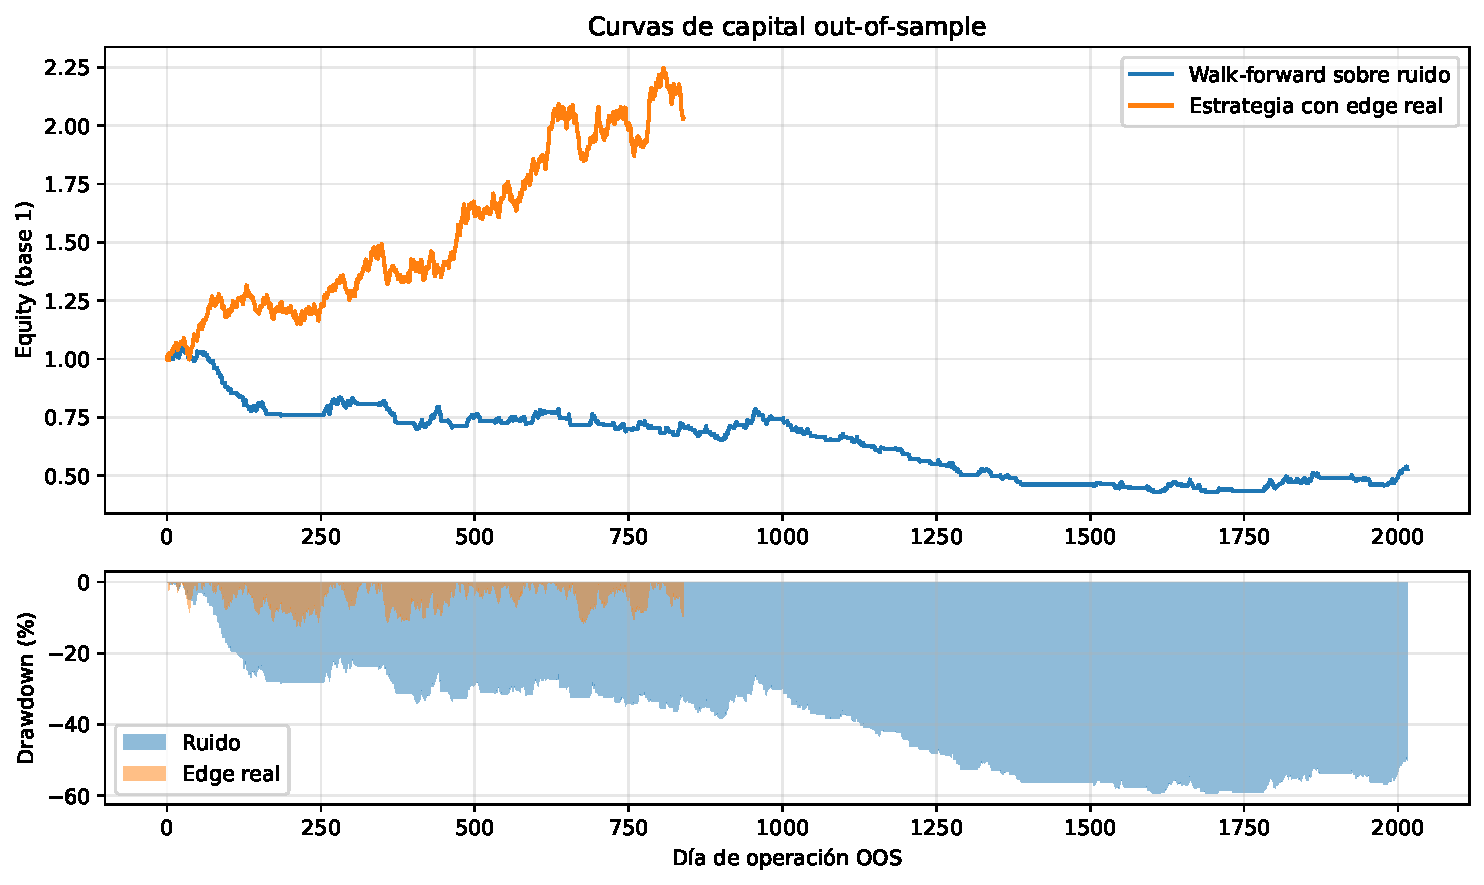
\includegraphics[keepaspectratio]{unidad3/cap17_backtesting_files/figure-pdf/equity-curve-output-1.pdf}}

Leé siempre la curva de capital junto con la de drawdown: el Sharpe
resume, pero la trayectoria muestra si las ganancias vinieron parejas o
de un golpe de suerte, y cuánto dolor (drawdown) hubo que aguantar en el
camino. Un inversor real abandona la estrategia en el fondo del drawdown
--- si ese fondo es -40\%, el Sharpe final es teoría.

\section{Los costos que el backtest
olvida}\label{los-costos-que-el-backtest-olvida}

Antes de creer cualquier número OOS, restale la realidad:

\begin{itemize}
\tightlist
\item
  \textbf{Costos de transacción y slippage}: una estrategia que rota
  mucho puede morir solo de comisiones. Simulá con costos por operación.
\item
  \textbf{Sesgo de supervivencia}: si tu universo actual excluye las
  empresas que quebraron, el pasado luce mejor de lo que fue.
\item
  \textbf{Look-ahead bias}: usar información que no estaba disponible en
  el momento de la decisión (balances publicados con retraso, precios de
  cierre para decidir ``durante'' el día).
\item
  \textbf{Capacidad}: el backtest asume que tus órdenes no mueven el
  precio; a mayor escala, deja de ser cierto.
\end{itemize}

\phantomsection\label{costos}
\begin{Shaded}
\begin{Highlighting}[]
\NormalTok{costo\_por\_operacion }\OperatorTok{=} \FloatTok{0.0005}   \CommentTok{\# 5 puntos básicos por cambio de posición}

\NormalTok{señal }\OperatorTok{=}\NormalTok{ np.array([test[}\BuiltInTok{max}\NormalTok{(}\DecValTok{0}\NormalTok{, t}\OperatorTok{{-}}\NormalTok{mejor\_v):t].mean() }\OperatorTok{\textgreater{}} \DecValTok{0} \ControlFlowTok{for}\NormalTok{ t }\KeywordTok{in} \BuiltInTok{range}\NormalTok{(}\BuiltInTok{len}\NormalTok{(test))])}
\NormalTok{cambios }\OperatorTok{=}\NormalTok{ np.}\BuiltInTok{abs}\NormalTok{(np.diff(señal.astype(}\BuiltInTok{int}\NormalTok{), prepend}\OperatorTok{=}\DecValTok{0}\NormalTok{))}
\NormalTok{r\_neto }\OperatorTok{=}\NormalTok{ np.where(señal, test, }\FloatTok{0.0}\NormalTok{) }\OperatorTok{{-}}\NormalTok{ cambios }\OperatorTok{*}\NormalTok{ costo\_por\_operacion}

\BuiltInTok{print}\NormalTok{(}\SpecialStringTok{f"Operaciones (cambios de posición): }\SpecialCharTok{\{}\NormalTok{cambios}\SpecialCharTok{.}\BuiltInTok{sum}\NormalTok{()}\SpecialCharTok{\}}\SpecialStringTok{"}\NormalTok{)}
\BuiltInTok{print}\NormalTok{(}\SpecialStringTok{f"Sharpe bruto: }\SpecialCharTok{\{}\NormalTok{sharpe(np.where(señal, test, }\FloatTok{0.0}\NormalTok{))}\SpecialCharTok{:.2f\}}\SpecialStringTok{"}\NormalTok{)}
\BuiltInTok{print}\NormalTok{(}\SpecialStringTok{f"Sharpe neto de costos: }\SpecialCharTok{\{}\NormalTok{sharpe(r\_neto)}\SpecialCharTok{:.2f\}}\SpecialStringTok{"}\NormalTok{)}
\end{Highlighting}
\end{Shaded}

\begin{verbatim}
Operaciones (cambios de posición): 111
Sharpe bruto: 0.16
Sharpe neto de costos: 0.03
\end{verbatim}

\begin{center}\rule{0.5\linewidth}{0.5pt}\end{center}

\chapter{El protocolo, en síntesis}\label{el-protocolo-en-suxedntesis}

Un backtest confiable sigue esta secuencia --- y el orden importa:

\begin{enumerate}
\def\labelenumi{\arabic{enumi}.}
\tightlist
\item
  \textbf{Hipótesis primero}: por qué debería funcionar (fundamento
  económico), antes de mirar datos.
\item
  \textbf{Diseño in-sample}, con la menor cantidad de parámetros
  posible.
\item
  \textbf{Contá tus intentos}: cada variante probada infla el umbral de
  significancia exigible.
\item
  \textbf{Walk-forward} para generar un track record 100\% OOS con
  recalibración realista.
\item
  \textbf{Costos, siempre}: comisiones, slippage, y los sesgos de datos.
\item
  \textbf{Inferencia honesta}: t-stat/p-value del track record OOS,
  corregido por múltiples pruebas.
\item
  \textbf{El OOS se usa una vez.} Si volvés a diseñar, necesitás datos
  nuevos (o esperar a que el mercado los genere).
\end{enumerate}

\begin{center}\rule{0.5\linewidth}{0.5pt}\end{center}

\chapter{Con datos reales}\label{con-datos-reales-3}

Todo el capítulo trabajó sobre ruido fabricado, donde sabíamos la
respuesta de antemano. El examen final es con datos donde \textbf{nadie}
sabe la respuesta: corremos el walk-forward completo sobre cinco años
del SPY, del dataset del libro (\texttt{datos/precios.csv}, ver
Apéndice~\ref{sec-datos-financieros}).

\phantomsection\label{wf-datos-reales}
\begin{Shaded}
\begin{Highlighting}[]
\NormalTok{precios }\OperatorTok{=}\NormalTok{ pd.read\_csv(}\StringTok{"../datos/precios.csv"}\NormalTok{, index\_col}\OperatorTok{=}\StringTok{"Date"}\NormalTok{, parse\_dates}\OperatorTok{=}\VariableTok{True}\NormalTok{)}
\NormalTok{r\_spy }\OperatorTok{=}\NormalTok{ precios[}\StringTok{"SPY"}\NormalTok{].pct\_change().dropna().values}

\NormalTok{oos\_spy, elec\_spy }\OperatorTok{=}\NormalTok{ walk\_forward(r\_spy, n\_train}\OperatorTok{=}\DecValTok{504}\NormalTok{, n\_test}\OperatorTok{=}\DecValTok{126}\NormalTok{, ventanas}\OperatorTok{=}\BuiltInTok{range}\NormalTok{(}\DecValTok{2}\NormalTok{, }\DecValTok{62}\NormalTok{))}

\BuiltInTok{print}\NormalTok{(}\SpecialStringTok{f"Tramos operados: }\SpecialCharTok{\{}\BuiltInTok{len}\NormalTok{(elec\_spy)}\SpecialCharTok{\}}\SpecialStringTok{ | Ventanas elegidas: }\SpecialCharTok{\{}\NormalTok{elec\_spy}\SpecialCharTok{\}}\SpecialStringTok{"}\NormalTok{)}
\NormalTok{evaluar(oos\_spy, }\StringTok{"Momentum SPY (walk{-}forward)"}\NormalTok{)}
\NormalTok{evaluar(r\_spy[}\OperatorTok{{-}}\BuiltInTok{len}\NormalTok{(oos\_spy):], }\StringTok{"Buy \& hold SPY (mismo período)"}\NormalTok{)}

\NormalTok{\_ }\OperatorTok{=}\NormalTok{ reporte(oos\_spy, }\StringTok{"Momentum SPY (OOS)"}\NormalTok{)}
\BuiltInTok{print}\NormalTok{()}
\NormalTok{\_ }\OperatorTok{=}\NormalTok{ reporte(r\_spy[}\OperatorTok{{-}}\BuiltInTok{len}\NormalTok{(oos\_spy):], }\StringTok{"Buy \& hold SPY"}\NormalTok{)}
\end{Highlighting}
\end{Shaded}

\begin{verbatim}
Tramos operados: 5 | Ventanas elegidas: [16, 10, 11, 9, 12]
Momentum SPY (walk-forward)  Sharpe:  0.92 | t:  1.45 | p-value: 0.149
Buy & hold SPY (mismo período) Sharpe:  1.31 | t:  2.07 | p-value: 0.039
— Momentum SPY (OOS)
  Sharpe:          0.92
  Retorno anual:   9.1%
  Máx. drawdown: -15.1%
  Hit ratio:      56.7%

— Buy & hold SPY
  Sharpe:          1.31
  Retorno anual:  20.8%
  Máx. drawdown: -18.8%
  Hit ratio:      57.5%
\end{verbatim}

Este resultado es una clase entera de honestidad estadística, así que
leelo despacio:

\begin{itemize}
\tightlist
\item
  \textbf{Las ventanas elegidas son estables entre tramos} --- nada del
  salto errático que vimos sobre ruido puro. Eso sugiere que el momentum
  del índice tiene \emph{algo} de estructura real.
\item
  El Sharpe out-of-sample es positivo, pero el \textbf{p-value no baja
  del umbral}: con \textasciitilde2.5 años de track record OOS, la
  fórmula \(t \approx \text{Sharpe} \times \sqrt{\text{años}}\) hace su
  trabajo implacable. Un Sharpe cercano a 1 con dos años y medio de
  datos \textbf{no es evidencia suficiente} --- verificalo vos mismo con
  la fórmula.
\item
  Y la comparación que un backtest siempre debe incluir: en el mismo
  período, \textbf{comprar y no hacer nada rindió más}. El período OOS
  fue mayormente alcista, y toda estrategia que pasa tiempo en cash paga
  ese costo. El consuelo del momentum es un drawdown máximo menor --- es
  una estrategia \emph{defensiva}, y su valor aparecería en un bear
  market largo, no en este tramo. Elegir el benchmark correcto es parte
  del protocolo.
\end{itemize}

Ah, y esto es \emph{antes} de costos de transacción. La conclusión
metodológica ---no sobre el momentum sino sobre el oficio--- es que un
backtest honesto casi nunca da un veredicto rotundo: da matices,
condiciones y un p-value incómodo. Desconfiá de los que no.

\begin{center}\rule{0.5\linewidth}{0.5pt}\end{center}

\chapter{Errores comunes}\label{errores-comunes-15}

\begin{tcolorbox}[enhanced jigsaw, bottomrule=.15mm, colback=white, opacitybacktitle=0.6, arc=.35mm, toprule=.15mm, opacityback=0, breakable, titlerule=0mm, left=2mm, coltitle=black, colbacktitle=quarto-callout-warning-color!10!white, colframe=quarto-callout-warning-color-frame, leftrule=.75mm, toptitle=1mm, bottomtitle=1mm, title=\textcolor{quarto-callout-warning-color}{\faExclamationTriangle}\hspace{0.5em}{Trampas frecuentes}, rightrule=.15mm]

\begin{itemize}
\tightlist
\item
  \textbf{Re-usar el out-of-sample}: la más común y la más letal. Cada
  iteración de ``ajusto y vuelvo a probar'' lo degrada a in-sample.
\item
  \textbf{Reportar el mejor de N sin decir N}: el Sharpe del mejor de
  100 intentos es una estadística de orden, no una medida de habilidad.
\item
  \textbf{Ignorar la estabilidad de los parámetros}: si el óptimo salta
  de 5 a 60 entre tramos del walk-forward, no estás estimando nada real.
\item
  \textbf{Backtests demasiado cortos}: recordá
  \(t \approx \text{Sharpe} \times \sqrt{\text{años}}\); con 2 años de
  datos casi nada es demostrable.
\item
  \textbf{Confundir el drawdown máximo del backtest con el peor caso
  posible}: el futuro no está obligado a repetir el peor pasado; es un
  piso, no un techo.
\end{itemize}

\end{tcolorbox}

\begin{center}\rule{0.5\linewidth}{0.5pt}\end{center}

\chapter{Ejercicios Propuestos}\label{ejercicios-propuestos-16}

\begin{tcolorbox}[enhanced jigsaw, bottomrule=.15mm, colback=white, opacitybacktitle=0.6, arc=.35mm, toprule=.15mm, opacityback=0, breakable, titlerule=0mm, left=2mm, coltitle=black, colbacktitle=quarto-callout-important-color!10!white, colframe=quarto-callout-important-color-frame, leftrule=.75mm, toptitle=1mm, bottomtitle=1mm, title=\textcolor{quarto-callout-important-color}{\faExclamation}\hspace{0.5em}{Ejercicios}, rightrule=.15mm]

\begin{enumerate}
\def\labelenumi{\arabic{enumi}.}
\tightlist
\item
  \textbf{La lotería de estrategias}: generá 100 series de ruido,
  ``optimizá'' la ventana de momentum en cada una y graficá el
  histograma de Sharpes in-sample del mejor parámetro. ¿Cuántos superan
  1.0?
\item
  \textbf{Bonferroni en acción}: con el experimento anterior, aplicá la
  corrección de Bonferroni (\(\alpha/60\)) al p-value del mejor Sharpe
  IS. ¿Sobrevive alguno?
\item
  \textbf{Walk-forward con edge}: sembrá una señal real débil (drift
  condicional a la señal de momentum) y verificá que el walk-forward la
  detecta: parámetros estables y Sharpe OOS positivo.
\item
  \textbf{Sensibilidad a costos}: para la estrategia con edge del
  capítulo, encontrá el costo por operación que lleva su Sharpe neto a
  cero. ¿Es un costo realista para un inversor minorista?
\item
  \textbf{Tu propio protocolo}: elegí una regla simple (cruce de medias
  móviles, por ejemplo), escribí la hipótesis económica ANTES de correr
  nada, y ejecutá el protocolo completo de 7 pasos sobre alguna de las
  acciones del dataset del libro (\texttt{datos/precios.csv}). Documentá
  cuántas variantes probaste.
\end{enumerate}

\end{tcolorbox}

Podés resolver estos ejercicios acá mismo: la celda ejecuta Python
\textbf{en tu navegador}, sin instalar nada (la primera ejecución tarda
unos segundos mientras carga el entorno; los paquetes que importes se
instalan solos).

\begin{Shaded}
\begin{Highlighting}[]
\NormalTok{\#| label: practica{-}navegador}
\NormalTok{import numpy as np}

\NormalTok{\# Para usar el dataset real del libro (requiere conexión):}
\NormalTok{\# import pandas as pd}
\NormalTok{\# from pyodide.http import open\_url}
\NormalTok{\# url = "https://diegoonna.github.io/libro\_finanzas\_computacionales/datos/precios.csv"}
\NormalTok{\# precios = pd.read\_csv(open\_url(url), index\_col="Date", parse\_dates=True)}

\NormalTok{\# Tu solución acá...}
\end{Highlighting}
\end{Shaded}

\begin{center}\rule{0.5\linewidth}{0.5pt}\end{center}

\chapter{Referencias}\label{referencias-16}

\phantomsection\label{refs}

\part{Módulo 4: Derivados y Volatilidad}

\chapter*{Módulo 4: Derivados y
Volatilidad}\label{muxf3dulo-4-derivados-y-volatilidad-1}
\addcontentsline{toc}{chapter}{Módulo 4: Derivados y Volatilidad}

\markboth{Módulo 4: Derivados y Volatilidad}{Módulo 4: Derivados y
Volatilidad}

\emph{El examen final: los derivados usan todo el libro a la vez}

Los derivados tienen fama de ser el tema más difícil de las finanzas, y
es una fama merecida --- pero no porque las ideas sean oscuras, sino
porque \textbf{usan todo a la vez}: probabilidad, simulación, métodos
numéricos, optimización y estructura de mercado, operando juntos en un
mismo instrumento. Por eso este módulo va al final: es el examen
integrador de todo lo que construiste en los tres anteriores.

La historia arranca con la pregunta más elegante de las finanzas del
siglo XX: \emph{¿cuánto vale el derecho de comprar algo en el futuro?}
La respuesta de \textbf{Black-Scholes} (Capítulo 18) es sorprendente: no
depende de lo que nadie opine sobre el mercado, porque la opción se
puede \emph{replicar} operando el activo subyacente. Implementamos la
fórmula, la damos vuelta para extraer la \textbf{volatilidad implícita}
de los precios reales, y nos topamos con el descubrimiento que cambió la
industria: la \textbf{sonrisa de volatilidad}, la evidencia de que el
mercado no le cree del todo al modelo.

Después bajamos al llano: el \textbf{delta hedging} (Capítulo 19) es la
réplica puesta en práctica, simulada día a día como la viviría un trader
--- con su error de cobertura, sus costos y el gamma mordiendo cerca del
vencimiento. Es, en el fondo, la demostración experimental de
Black-Scholes. Y el cierre (Capítulo 20) enfrenta lo que la sonrisa
venía gritando: la volatilidad no es una constante, es un proceso con
vida propia. Los modelos de \textbf{Heston} y \textbf{SABR} la tratan
como tal, reproducen la sonrisa desde los fundamentos, y son la puerta
de entrada al pricing profesional moderno.

\begin{tcolorbox}[enhanced jigsaw, bottomrule=.15mm, colback=white, breakable, left=2mm, colframe=quarto-callout-note-color-frame, leftrule=.75mm, arc=.35mm, toprule=.15mm, rightrule=.15mm, opacityback=0]
\begin{minipage}[t]{5.5mm}
\textcolor{quarto-callout-note-color}{\faInfo}
\end{minipage}%
\begin{minipage}[t]{\textwidth - 5.5mm}

\vspace{-3mm}\textbf{Qué necesitás tener fresco}\vspace{3mm}

Este módulo apoya todo su peso sobre la simulación de Monte Carlo y el
GBM (Capítulo 13), los procesos con saltos (Capítulo 14) y las nociones
de colas y curtosis (Capítulos 7 y 11). Si venís directo, perfecto; si
no, un repaso rápido de esos capítulos hace que este módulo fluya.

\end{minipage}%
\end{tcolorbox}

\begin{center}\rule{0.5\linewidth}{0.5pt}\end{center}

\section*{🎯 Objetivos de Aprendizaje}\label{objetivos-de-aprendizaje-3}
\addcontentsline{toc}{section}{🎯 Objetivos de Aprendizaje}

\markright{🎯 Objetivos de Aprendizaje}

Al completar este módulo, vas a ser capaz de:

\begin{enumerate}
\def\labelenumi{\arabic{enumi}.}
\tightlist
\item
  \textbf{Implementar la fórmula de Black-Scholes} para calls y puts
  europeas.
\item
  \textbf{Extraer volatilidad implícita} de precios de mercado usando
  Newton-Raphson.
\item
  \textbf{Calcular las griegas} (Delta, Gamma, Vega, Theta) analítica y
  numéricamente.
\item
  \textbf{Simular delta hedging dinámico} y analizar su P\&L y su error
  de cobertura.
\item
  \textbf{Modelar la volatilidad estocástica} con Heston y SABR para
  capturar la sonrisa.
\end{enumerate}

\begin{center}\rule{0.5\linewidth}{0.5pt}\end{center}

\section*{🗓️ Recorrido Capítulo a
Capítulo}\label{recorrido-capuxedtulo-a-capuxedtulo-3}
\addcontentsline{toc}{section}{🗓️ Recorrido Capítulo a Capítulo}

\markright{🗓️ Recorrido Capítulo a Capítulo}

\begin{longtable}[]{@{}
  >{\centering\arraybackslash}p{(\linewidth - 6\tabcolsep) * \real{0.2500}}
  >{\raggedright\arraybackslash}p{(\linewidth - 6\tabcolsep) * \real{0.1875}}
  >{\raggedright\arraybackslash}p{(\linewidth - 6\tabcolsep) * \real{0.2500}}
  >{\raggedright\arraybackslash}p{(\linewidth - 6\tabcolsep) * \real{0.3125}}@{}}
\toprule\noalign{}
\begin{minipage}[b]{\linewidth}\centering
Capítulo
\end{minipage} & \begin{minipage}[b]{\linewidth}\raggedright
Tema
\end{minipage} & \begin{minipage}[b]{\linewidth}\raggedright
Python
\end{minipage} & \begin{minipage}[b]{\linewidth}\raggedright
Finanzas
\end{minipage} \\
\midrule\noalign{}
\endhead
\bottomrule\noalign{}
\endlastfoot
\textbf{18} & Derivados y Vol Implícita & \texttt{scipy.stats.norm},
iteración numérica & Black-Scholes, smile, griegas \\
\textbf{19} & Delta Hedging & Simulación de trading, DataFrames &
Cobertura dinámica, P\&L, riesgo gamma \\
\textbf{20} & Volatilidad Estocástica & Simulación de procesos acoplados
& Heston, SABR, superficie de volatilidad \\
\end{longtable}

\begin{center}\rule{0.5\linewidth}{0.5pt}\end{center}

\section*{🧰 Herramientas y
Librerías}\label{herramientas-y-libreruxedas-3}
\addcontentsline{toc}{section}{🧰 Herramientas y Librerías}

\markright{🧰 Herramientas y Librerías}

\textbf{SciPy}

\texttt{norm.cdf}, \texttt{norm.pdf}

\textbf{NumPy}

Simulación vectorizada

\textbf{Pandas}

Logging de operaciones

\textbf{Matplotlib}

Payoffs, smile, P\&L

\begin{center}\rule{0.5\linewidth}{0.5pt}\end{center}

\section*{🔑 Concepto Clave:
Black-Scholes}\label{concepto-clave-black-scholes}
\addcontentsline{toc}{section}{🔑 Concepto Clave: Black-Scholes}

\markright{🔑 Concepto Clave: Black-Scholes}

\begin{tcolorbox}[enhanced jigsaw, bottomrule=.15mm, colback=white, breakable, left=2mm, colframe=quarto-callout-important-color-frame, leftrule=.75mm, arc=.35mm, toprule=.15mm, rightrule=.15mm, opacityback=0]
\begin{minipage}[t]{5.5mm}
\textcolor{quarto-callout-important-color}{\faExclamation}
\end{minipage}%
\begin{minipage}[t]{\textwidth - 5.5mm}

La fórmula de \textbf{Black-Scholes} para una call europea:

\[C = S_0 \, N(d_1) - K \, e^{-rT} \, N(d_2)\]

\[d_1 = \frac{\ln(S_0/K) + (r + \sigma^2/2)T}{\sigma\sqrt{T}}, \quad d_2 = d_1 - \sigma\sqrt{T}\]

Black-Scholes asume volatilidad constante, pero el mercado revela una
\textbf{sonrisa de volatilidad} que contradice ese supuesto. El módulo
entero puede leerse como esa tensión: primero la fórmula, después su uso
real, y al final los modelos que reparan lo que le falta.

\end{minipage}%
\end{tcolorbox}

\begin{center}\rule{0.5\linewidth}{0.5pt}\end{center}

\section*{📚 Lecturas Recomendadas}\label{lecturas-recomendadas-3}
\addcontentsline{toc}{section}{📚 Lecturas Recomendadas}

\markright{📚 Lecturas Recomendadas}

\begin{itemize}
\tightlist
\item
  Hull, J. (2018). \emph{Options, Futures, and Other Derivatives}.
  Pearson.
\item
  Wilmott, P. (2006). \emph{Paul Wilmott on Quantitative Finance}.
  Wiley.
\item
  Taleb, N. N. (1997). \emph{Dynamic Hedging}. Wiley.
\item
  Gatheral, J. (2006). \emph{The Volatility Surface: A Practitioner's
  Guide}. Wiley.
\end{itemize}

\chapter{Capítulo 18: Valuación de Opciones y Volatilidad
Implícita}\label{capuxedtulo-18-valuaciuxf3n-de-opciones-y-volatilidad-impluxedcita}

Black-Scholes, Newton-Raphson, la sonrisa y las griegas

Las opciones son el laboratorio perfecto de las finanzas cuantitativas:
juntan probabilidad, métodos numéricos y estructura de mercado en un
solo instrumento. Implementamos la fórmula de Black-Scholes, invertimos
el problema para extraer la volatilidad implícita con Newton-Raphson,
descubrimos la sonrisa de volatilidad ---la evidencia de que el mercado
no le cree a Black-Scholes--- y calculamos las griegas, los tableros de
sensibilidad que gobiernan la gestión de un book de opciones.

\hfill\break

\chapter{Introducción}\label{introducciuxf3n-15}

Una \textbf{opción de compra} (\emph{call}) da el derecho ---no la
obligación--- de comprar un activo a un precio pactado \(K\) (el
\emph{strike}) en una fecha futura \(T\). Una \emph{put}, el derecho de
vender. La pregunta que define al capítulo: \textbf{¿cuánto vale hoy ese
derecho?}

La respuesta tiene una historia célebre. En 1973, Fischer Black, Myron
Scholes y Robert Merton demostraron que ---bajo ciertos supuestos--- el
precio de una opción \textbf{no depende de la expectativa de nadie}
sobre si el activo va a subir o bajar. Depende de algo más sutil: de que
la opción se puede \emph{replicar} comprando y vendiendo dinámicamente
el activo subyacente. Y si dos cosas tienen los mismos flujos, deben
valer lo mismo (no-arbitraje). De esa lógica sale una fórmula cerrada,
la más famosa de las finanzas.

En este capítulo la implementamos, y enseguida la damos vuelta: en el
mercado real, la fórmula no se usa para calcular precios (los precios se
\emph{observan} en pantalla) sino para traducirlos a un lenguaje común:
la \textbf{volatilidad implícita}.

\phantomsection\label{setup}
\begin{Shaded}
\begin{Highlighting}[]
\ImportTok{import}\NormalTok{ numpy }\ImportTok{as}\NormalTok{ np}
\ImportTok{import}\NormalTok{ matplotlib.pyplot }\ImportTok{as}\NormalTok{ plt}
\ImportTok{from}\NormalTok{ scipy.stats }\ImportTok{import}\NormalTok{ norm}
\end{Highlighting}
\end{Shaded}

\begin{center}\rule{0.5\linewidth}{0.5pt}\end{center}

\chapter{La fórmula de
Black-Scholes}\label{la-fuxf3rmula-de-black-scholes}

Para una call europea sobre un activo que sigue un GBM (Capítulo 13) con
volatilidad \(\sigma\), con tasa libre de riesgo \(r\):

\[C = S_0\, N(d_1) - K e^{-rT} N(d_2)\]

\[d_1 = \frac{\ln(S_0/K) + (r + \sigma^2/2)\,T}{\sigma\sqrt{T}}, \qquad d_2 = d_1 - \sigma\sqrt{T}\]

donde \(N(\cdot)\) es la función de distribución normal estándar. La
fórmula tiene una lectura económica directa que ayuda a memorizarla: es
\textbf{lo que recibís menos lo que pagás, ponderado por probabilidades}
(en el mundo neutral al riesgo): \(N(d_2)\) es la probabilidad de
ejercer, \(K e^{-rT} N(d_2)\) el valor presente esperado de lo que pagás
si ejercés, y \(S_0 N(d_1)\) el valor esperado de lo que recibís.

\phantomsection\label{bsm}
\begin{Shaded}
\begin{Highlighting}[]
\KeywordTok{def}\NormalTok{ bs\_call(S, K, T, r, sigma):}
    \CommentTok{"""Precio Black{-}Scholes de una call europea."""}
\NormalTok{    d1 }\OperatorTok{=}\NormalTok{ (np.log(S }\OperatorTok{/}\NormalTok{ K) }\OperatorTok{+}\NormalTok{ (r }\OperatorTok{+} \FloatTok{0.5} \OperatorTok{*}\NormalTok{ sigma}\OperatorTok{**}\DecValTok{2}\NormalTok{) }\OperatorTok{*}\NormalTok{ T) }\OperatorTok{/}\NormalTok{ (sigma }\OperatorTok{*}\NormalTok{ np.sqrt(T))}
\NormalTok{    d2 }\OperatorTok{=}\NormalTok{ d1 }\OperatorTok{{-}}\NormalTok{ sigma }\OperatorTok{*}\NormalTok{ np.sqrt(T)}
    \ControlFlowTok{return}\NormalTok{ S }\OperatorTok{*}\NormalTok{ norm.cdf(d1) }\OperatorTok{{-}}\NormalTok{ K }\OperatorTok{*}\NormalTok{ np.exp(}\OperatorTok{{-}}\NormalTok{r }\OperatorTok{*}\NormalTok{ T) }\OperatorTok{*}\NormalTok{ norm.cdf(d2)}

\KeywordTok{def}\NormalTok{ bs\_put(S, K, T, r, sigma):}
    \CommentTok{"""Precio Black{-}Scholes de una put europea."""}
\NormalTok{    d1 }\OperatorTok{=}\NormalTok{ (np.log(S }\OperatorTok{/}\NormalTok{ K) }\OperatorTok{+}\NormalTok{ (r }\OperatorTok{+} \FloatTok{0.5} \OperatorTok{*}\NormalTok{ sigma}\OperatorTok{**}\DecValTok{2}\NormalTok{) }\OperatorTok{*}\NormalTok{ T) }\OperatorTok{/}\NormalTok{ (sigma }\OperatorTok{*}\NormalTok{ np.sqrt(T))}
\NormalTok{    d2 }\OperatorTok{=}\NormalTok{ d1 }\OperatorTok{{-}}\NormalTok{ sigma }\OperatorTok{*}\NormalTok{ np.sqrt(T)}
    \ControlFlowTok{return}\NormalTok{ K }\OperatorTok{*}\NormalTok{ np.exp(}\OperatorTok{{-}}\NormalTok{r }\OperatorTok{*}\NormalTok{ T) }\OperatorTok{*}\NormalTok{ norm.cdf(}\OperatorTok{{-}}\NormalTok{d2) }\OperatorTok{{-}}\NormalTok{ S }\OperatorTok{*}\NormalTok{ norm.cdf(}\OperatorTok{{-}}\NormalTok{d1)}

\CommentTok{\# Un contrato concreto: call al dinero, 6 meses, vol 25\%}
\NormalTok{S, K, T, r, sigma }\OperatorTok{=} \DecValTok{100}\NormalTok{, }\DecValTok{100}\NormalTok{, }\FloatTok{0.5}\NormalTok{, }\FloatTok{0.05}\NormalTok{, }\FloatTok{0.25}

\NormalTok{precio\_call }\OperatorTok{=}\NormalTok{ bs\_call(S, K, T, r, sigma)}
\NormalTok{precio\_put }\OperatorTok{=}\NormalTok{ bs\_put(S, K, T, r, sigma)}

\BuiltInTok{print}\NormalTok{(}\SpecialStringTok{f"Call: $}\SpecialCharTok{\{}\NormalTok{precio\_call}\SpecialCharTok{:.4f\}}\SpecialStringTok{"}\NormalTok{)}
\BuiltInTok{print}\NormalTok{(}\SpecialStringTok{f"Put:  $}\SpecialCharTok{\{}\NormalTok{precio\_put}\SpecialCharTok{:.4f\}}\SpecialStringTok{"}\NormalTok{)}
\BuiltInTok{print}\NormalTok{(}\SpecialStringTok{f"}\CharTok{\textbackslash{}n}\SpecialStringTok{Verificación de paridad put{-}call:"}\NormalTok{)}
\BuiltInTok{print}\NormalTok{(}\SpecialStringTok{f"  C {-} P           = }\SpecialCharTok{\{}\NormalTok{precio\_call }\OperatorTok{{-}}\NormalTok{ precio\_put}\SpecialCharTok{:.4f\}}\SpecialStringTok{"}\NormalTok{)}
\BuiltInTok{print}\NormalTok{(}\SpecialStringTok{f"  S {-} K·e\^{}({-}rT)   = }\SpecialCharTok{\{}\NormalTok{S }\OperatorTok{{-}}\NormalTok{ K }\OperatorTok{*}\NormalTok{ np}\SpecialCharTok{.}\NormalTok{exp(}\OperatorTok{{-}}\NormalTok{r }\OperatorTok{*}\NormalTok{ T)}\SpecialCharTok{:.4f\}}\SpecialStringTok{"}\NormalTok{)}
\end{Highlighting}
\end{Shaded}

\begin{verbatim}
Call: $8.2600
Put:  $5.7910

Verificación de paridad put-call:
  C - P           = 2.4690
  S - K·e^(-rT)   = 2.4690
\end{verbatim}

La \textbf{paridad put-call} (\(C - P = S - Ke^{-rT}\)) que verificamos
al final no depende de Black-Scholes ni de ningún modelo: sale de puro
no-arbitraje. Por eso es el primer chequeo de cordura de cualquier
implementación --- si tu código la viola, está mal.

\begin{tcolorbox}[enhanced jigsaw, bottomrule=.15mm, colback=white, opacitybacktitle=0.6, arc=.35mm, toprule=.15mm, opacityback=0, breakable, titlerule=0mm, left=2mm, coltitle=black, colbacktitle=quarto-callout-note-color!10!white, colframe=quarto-callout-note-color-frame, leftrule=.75mm, toptitle=1mm, bottomtitle=1mm, title=\textcolor{quarto-callout-note-color}{\faInfo}\hspace{0.5em}{Los supuestos que después importarán}, rightrule=.15mm]

Black-Scholes supone: volatilidad \(\sigma\) \textbf{constante y
conocida}, trayectorias continuas (sin saltos --- ya sabemos por el
Capítulo 14 que es falso), tasa constante, sin costos de transacción y
posibilidad de operar continuamente. Cada supuesto se viola en la
realidad, y la genialidad práctica del mercado fue inventar una forma de
\emph{medir} esas violaciones: la sonrisa de volatilidad que veremos
enseguida.

\end{tcolorbox}

\section{¿Qué mueve el precio de una
opción?}\label{quuxe9-mueve-el-precio-de-una-opciuxf3n}

Antes de invertir la fórmula, desarrollemos intuición sobre cómo
responde el precio a sus inputs:

\begin{Shaded}
\begin{Highlighting}[]
\NormalTok{S\_grid }\OperatorTok{=}\NormalTok{ np.linspace(}\DecValTok{60}\NormalTok{, }\DecValTok{140}\NormalTok{, }\DecValTok{100}\NormalTok{)}

\NormalTok{fig, axes }\OperatorTok{=}\NormalTok{ plt.subplots(}\DecValTok{1}\NormalTok{, }\DecValTok{2}\NormalTok{, figsize}\OperatorTok{=}\NormalTok{(}\DecValTok{11}\NormalTok{, }\DecValTok{4}\NormalTok{))}

\CommentTok{\# Panel 1: valor de la call vs precio del subyacente, a distintos plazos}
\NormalTok{ax }\OperatorTok{=}\NormalTok{ axes[}\DecValTok{0}\NormalTok{]}
\ControlFlowTok{for}\NormalTok{ T\_i, estilo }\KeywordTok{in}\NormalTok{ [(}\FloatTok{0.05}\NormalTok{, }\StringTok{":"}\NormalTok{), (}\FloatTok{0.25}\NormalTok{, }\StringTok{"{-}{-}"}\NormalTok{), (}\FloatTok{1.0}\NormalTok{, }\StringTok{"{-}"}\NormalTok{)]:}
\NormalTok{    ax.plot(S\_grid, bs\_call(S\_grid, K, T\_i, r, sigma), estilo,}
\NormalTok{            label}\OperatorTok{=}\SpecialStringTok{f"T = }\SpecialCharTok{\{}\NormalTok{T\_i}\SpecialCharTok{\}}\SpecialStringTok{ años"}\NormalTok{)}
\NormalTok{ax.plot(S\_grid, np.maximum(S\_grid }\OperatorTok{{-}}\NormalTok{ K, }\DecValTok{0}\NormalTok{), }\StringTok{"k{-}"}\NormalTok{, alpha}\OperatorTok{=}\FloatTok{0.3}\NormalTok{, linewidth}\OperatorTok{=}\DecValTok{3}\NormalTok{,}
\NormalTok{        label}\OperatorTok{=}\StringTok{"Payoff al vencimiento"}\NormalTok{)}
\NormalTok{ax.set\_xlabel(}\StringTok{"Precio del subyacente S"}\NormalTok{)}
\NormalTok{ax.set\_ylabel(}\StringTok{"Valor de la call"}\NormalTok{)}
\NormalTok{ax.set\_title(}\StringTok{"El tiempo \textquotesingle{}redondea\textquotesingle{} el payoff"}\NormalTok{)}
\NormalTok{ax.legend()}
\NormalTok{ax.grid(}\VariableTok{True}\NormalTok{, alpha}\OperatorTok{=}\FloatTok{0.3}\NormalTok{)}

\CommentTok{\# Panel 2: valor vs volatilidad}
\NormalTok{ax }\OperatorTok{=}\NormalTok{ axes[}\DecValTok{1}\NormalTok{]}
\NormalTok{vol\_grid }\OperatorTok{=}\NormalTok{ np.linspace(}\FloatTok{0.05}\NormalTok{, }\FloatTok{0.60}\NormalTok{, }\DecValTok{100}\NormalTok{)}
\ControlFlowTok{for}\NormalTok{ K\_i }\KeywordTok{in}\NormalTok{ [}\DecValTok{90}\NormalTok{, }\DecValTok{100}\NormalTok{, }\DecValTok{110}\NormalTok{]:}
\NormalTok{    ax.plot(vol\_grid }\OperatorTok{*} \DecValTok{100}\NormalTok{, bs\_call(S, K\_i, T, r, vol\_grid), label}\OperatorTok{=}\SpecialStringTok{f"K = }\SpecialCharTok{\{}\NormalTok{K\_i}\SpecialCharTok{\}}\SpecialStringTok{"}\NormalTok{)}
\NormalTok{ax.set\_xlabel(}\StringTok{"Volatilidad σ (\%)"}\NormalTok{)}
\NormalTok{ax.set\_ylabel(}\StringTok{"Valor de la call"}\NormalTok{)}
\NormalTok{ax.set\_title(}\StringTok{"Más volatilidad, más valor — siempre"}\NormalTok{)}
\NormalTok{ax.legend()}
\NormalTok{ax.grid(}\VariableTok{True}\NormalTok{, alpha}\OperatorTok{=}\FloatTok{0.3}\NormalTok{)}

\NormalTok{plt.tight\_layout()}
\NormalTok{plt.show()}
\end{Highlighting}
\end{Shaded}

\pandocbounded{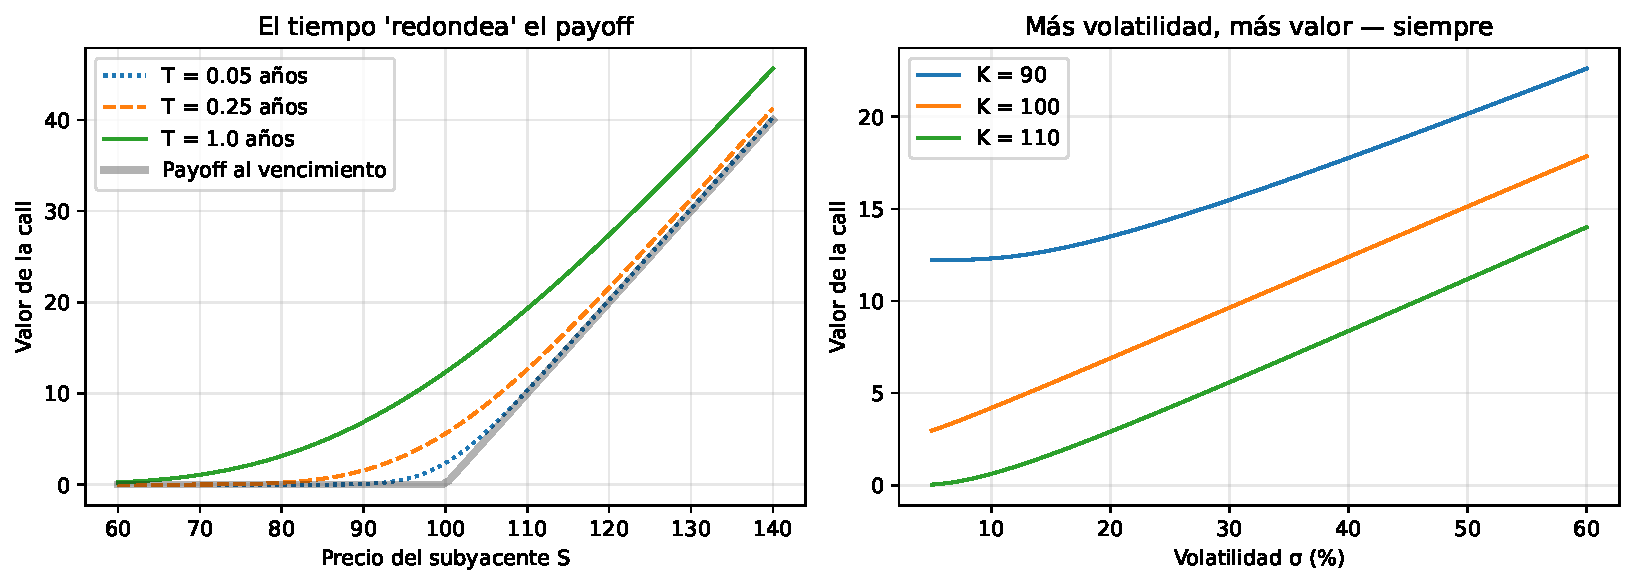
\includegraphics[keepaspectratio]{unidad4/cap18_derivados_vol_implicita_files/figure-pdf/sensibilidad-visual-output-1.pdf}}

El panel derecho contiene la clave de todo el capítulo: \textbf{el
precio de una opción crece monótonamente con la volatilidad}. Tiene
sentido económico: la opción te protege de la baja (perdés como mucho la
prima) y te deja toda la suba --- más dispersión solo puede favorecerte.
Esa monotonía significa que la relación precio ↔ volatilidad es
\textbf{uno a uno}: dado un precio, existe una única \(\sigma\) que lo
genera. Podemos invertir la fórmula.

\begin{center}\rule{0.5\linewidth}{0.5pt}\end{center}

\chapter{Volatilidad implícita: leer la fórmula al
revés}\label{volatilidad-impluxedcita-leer-la-fuxf3rmula-al-revuxe9s}

En el mercado, el precio de la opción se \textbf{observa} --- lo pone la
oferta y la demanda. De los cinco inputs de Black-Scholes, cuatro son
observables (\(S\), \(K\), \(T\), \(r\)). El único invisible es
\(\sigma\). Entonces el uso real de la fórmula es el inverso: \emph{¿qué
volatilidad está ``implicando'' este precio de mercado?}

\[\sigma_{impl} : \quad C_{BS}(S, K, T, r, \sigma_{impl}) = C_{mercado}\]

No hay fórmula cerrada para despejar \(\sigma\); hay que resolver
numéricamente. El método clásico es \textbf{Newton-Raphson}: arrancar de
un \(\sigma\) tentativo y corregirlo usando la pendiente de la función,

\[\sigma_{n+1} = \sigma_n - \frac{C_{BS}(\sigma_n) - C_{mercado}}{\partial C / \partial \sigma}\]

donde la derivada del denominador tiene nombre propio
---\textbf{vega}--- y fórmula cerrada. Cada iteración pregunta: ``¿me
pasé o me quedé corto? ¿y cuán sensible es el precio acá?'' y da un paso
proporcional al error.

\phantomsection\label{vol-implicita}
\begin{Shaded}
\begin{Highlighting}[]
\KeywordTok{def}\NormalTok{ vega(S, K, T, r, sigma):}
    \CommentTok{"""Vega: derivada del precio respecto de la volatilidad."""}
\NormalTok{    d1 }\OperatorTok{=}\NormalTok{ (np.log(S }\OperatorTok{/}\NormalTok{ K) }\OperatorTok{+}\NormalTok{ (r }\OperatorTok{+} \FloatTok{0.5} \OperatorTok{*}\NormalTok{ sigma}\OperatorTok{**}\DecValTok{2}\NormalTok{) }\OperatorTok{*}\NormalTok{ T) }\OperatorTok{/}\NormalTok{ (sigma }\OperatorTok{*}\NormalTok{ np.sqrt(T))}
    \ControlFlowTok{return}\NormalTok{ S }\OperatorTok{*}\NormalTok{ np.sqrt(T) }\OperatorTok{*}\NormalTok{ norm.pdf(d1)}

\KeywordTok{def}\NormalTok{ implied\_vol(precio\_mercado, S, K, T, r, sigma0}\OperatorTok{=}\FloatTok{0.3}\NormalTok{, tol}\OperatorTok{=}\FloatTok{1e{-}8}\NormalTok{, max\_iter}\OperatorTok{=}\DecValTok{100}\NormalTok{):}
    \CommentTok{"""Volatilidad implícita de una call por Newton{-}Raphson."""}
\NormalTok{    sigma }\OperatorTok{=}\NormalTok{ sigma0}
    \ControlFlowTok{for}\NormalTok{ \_ }\KeywordTok{in} \BuiltInTok{range}\NormalTok{(max\_iter):}
\NormalTok{        diff }\OperatorTok{=}\NormalTok{ bs\_call(S, K, T, r, sigma) }\OperatorTok{{-}}\NormalTok{ precio\_mercado}
        \ControlFlowTok{if} \BuiltInTok{abs}\NormalTok{(diff) }\OperatorTok{\textless{}}\NormalTok{ tol:}
            \ControlFlowTok{return}\NormalTok{ sigma}
\NormalTok{        v }\OperatorTok{=}\NormalTok{ vega(S, K, T, r, sigma)}
        \ControlFlowTok{if}\NormalTok{ v }\OperatorTok{\textless{}} \FloatTok{1e{-}12}\NormalTok{:                      }\CommentTok{\# vega \textasciitilde{}0: Newton se queda sin pendiente}
            \ControlFlowTok{raise} \PreprocessorTok{RuntimeError}\NormalTok{(}\StringTok{"Vega demasiado chica; usar bisección/brentq"}\NormalTok{)}
\NormalTok{        sigma }\OperatorTok{{-}=}\NormalTok{ diff }\OperatorTok{/}\NormalTok{ v}
    \ControlFlowTok{raise} \PreprocessorTok{RuntimeError}\NormalTok{(}\StringTok{"No convergió"}\NormalTok{)}

\CommentTok{\# Test de ida y vuelta: precio generado con σ=30\% → ¿recuperamos 30\%?}
\NormalTok{precio\_test }\OperatorTok{=}\NormalTok{ bs\_call(}\DecValTok{100}\NormalTok{, }\DecValTok{100}\NormalTok{, }\FloatTok{0.5}\NormalTok{, }\FloatTok{0.05}\NormalTok{, }\FloatTok{0.30}\NormalTok{)}
\NormalTok{vol\_recuperada }\OperatorTok{=}\NormalTok{ implied\_vol(precio\_test, }\DecValTok{100}\NormalTok{, }\DecValTok{100}\NormalTok{, }\FloatTok{0.5}\NormalTok{, }\FloatTok{0.05}\NormalTok{)}
\BuiltInTok{print}\NormalTok{(}\SpecialStringTok{f"σ original: 30.00\%  →  σ recuperada: }\SpecialCharTok{\{}\NormalTok{vol\_recuperada}\SpecialCharTok{:.4\%\}}\SpecialStringTok{"}\NormalTok{)}
\end{Highlighting}
\end{Shaded}

\begin{verbatim}
σ original: 30.00%  →  σ recuperada: 30.0000%
\end{verbatim}

Newton converge en un puñado de iteraciones porque el precio es suave y
monótono en \(\sigma\). La volatilidad implícita es \textbf{el idioma en
que se cotizan las opciones}: los operadores no dicen ``la call vale
\$8.26'', dicen ``está en 30 de vol'' --- un número comparable entre
strikes, plazos y subyacentes.

\begin{center}\rule{0.5\linewidth}{0.5pt}\end{center}

\chapter{La sonrisa de volatilidad}\label{la-sonrisa-de-volatilidad}

Y acá viene el descubrimiento que cambió la industria. Si Black-Scholes
fuera literalmente cierto, la volatilidad implícita sería \textbf{la
misma para todos los strikes} --- es un parámetro del activo, no del
contrato. Grafiquemos qué se observa en el mercado real:

\begin{Shaded}
\begin{Highlighting}[]
\NormalTok{strikes }\OperatorTok{=}\NormalTok{ np.arange(}\DecValTok{80}\NormalTok{, }\DecValTok{121}\NormalTok{, }\DecValTok{2}\NormalTok{)}
\NormalTok{S, T, r }\OperatorTok{=} \DecValTok{100}\NormalTok{, }\FloatTok{0.5}\NormalTok{, }\FloatTok{0.05}

\CommentTok{\# El mercado cotiza opciones fuera del dinero más "caras" (en vol):}
\CommentTok{\# reproducimos precios de mercado con una vol que depende del strike}
\NormalTok{vols\_mercado }\OperatorTok{=} \FloatTok{0.20} \OperatorTok{+} \FloatTok{0.001} \OperatorTok{*}\NormalTok{ (strikes }\OperatorTok{{-}} \DecValTok{100}\NormalTok{) }\OperatorTok{**} \DecValTok{2} \OperatorTok{+} \FloatTok{0.0015} \OperatorTok{*}\NormalTok{ np.maximum(}\DecValTok{100} \OperatorTok{{-}}\NormalTok{ strikes, }\DecValTok{0}\NormalTok{)}
\NormalTok{precios\_mkt }\OperatorTok{=}\NormalTok{ [bs\_call(S, K\_i, T, r, v) }\ControlFlowTok{for}\NormalTok{ K\_i, v }\KeywordTok{in} \BuiltInTok{zip}\NormalTok{(strikes, vols\_mercado)]}

\CommentTok{\# Recuperamos la vol implícita de cada precio (así se construye el gráfico real)}
\NormalTok{vols\_impl }\OperatorTok{=}\NormalTok{ [implied\_vol(p, S, K\_i, T, r) }\ControlFlowTok{for}\NormalTok{ p, K\_i }\KeywordTok{in} \BuiltInTok{zip}\NormalTok{(precios\_mkt, strikes)]}

\NormalTok{fig, ax }\OperatorTok{=}\NormalTok{ plt.subplots(figsize}\OperatorTok{=}\NormalTok{(}\DecValTok{9}\NormalTok{, }\DecValTok{5}\NormalTok{))}
\NormalTok{ax.plot(strikes, np.array(vols\_impl) }\OperatorTok{*} \DecValTok{100}\NormalTok{, }\StringTok{"o{-}"}\NormalTok{, color}\OperatorTok{=}\StringTok{"steelblue"}\NormalTok{,}
\NormalTok{        label}\OperatorTok{=}\StringTok{"Vol implícita observada"}\NormalTok{)}
\NormalTok{ax.axhline(}\DecValTok{20}\NormalTok{, color}\OperatorTok{=}\StringTok{"red"}\NormalTok{, linestyle}\OperatorTok{=}\StringTok{"{-}{-}"}\NormalTok{, alpha}\OperatorTok{=}\FloatTok{0.6}\NormalTok{,}
\NormalTok{           label}\OperatorTok{=}\StringTok{"Lo que Black{-}Scholes predice (σ constante)"}\NormalTok{)}
\NormalTok{ax.axvline(}\DecValTok{100}\NormalTok{, color}\OperatorTok{=}\StringTok{"gray"}\NormalTok{, linestyle}\OperatorTok{=}\StringTok{":"}\NormalTok{, alpha}\OperatorTok{=}\FloatTok{0.5}\NormalTok{)}
\NormalTok{ax.annotate(}\StringTok{"puts protectivas}\CharTok{\textbackslash{}n}\StringTok{(caras)"}\NormalTok{, xy}\OperatorTok{=}\NormalTok{(}\DecValTok{84}\NormalTok{, }\FloatTok{24.5}\NormalTok{), fontsize}\OperatorTok{=}\DecValTok{9}\NormalTok{, ha}\OperatorTok{=}\StringTok{"center"}\NormalTok{)}
\NormalTok{ax.set\_xlabel(}\StringTok{"Strike K"}\NormalTok{)}
\NormalTok{ax.set\_ylabel(}\StringTok{"Volatilidad implícita (\%)"}\NormalTok{)}
\NormalTok{ax.set\_title(}\StringTok{"La sonrisa (smirk) de volatilidad"}\NormalTok{)}
\NormalTok{ax.legend()}
\NormalTok{ax.grid(}\VariableTok{True}\NormalTok{, alpha}\OperatorTok{=}\FloatTok{0.3}\NormalTok{)}
\NormalTok{plt.tight\_layout()}
\NormalTok{plt.show()}
\end{Highlighting}
\end{Shaded}

\pandocbounded{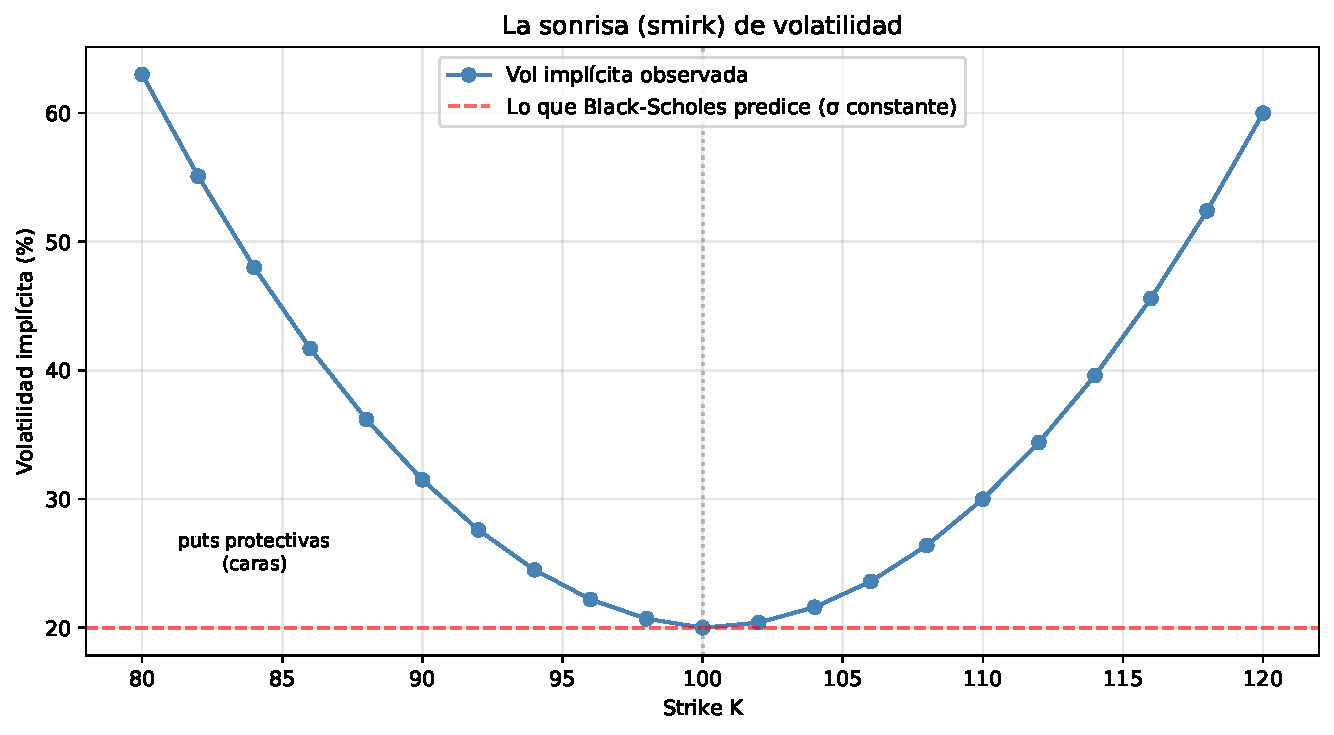
\includegraphics[keepaspectratio]{unidad4/cap18_derivados_vol_implicita_files/figure-pdf/smile-output-1.pdf}}

La curva no es plana: las opciones \textbf{fuera del dinero se cotizan a
volatilidades más altas}, con la rama izquierda (puts de strikes bajos)
típicamente más empinada --- por su forma, \emph{sonrisa} o \emph{mueca}
(smirk). ¿Qué está diciendo el mercado?

\begin{itemize}
\tightlist
\item
  \textbf{Las colas existen}: los compradores pagan más (en vol) por las
  opciones que pagan en escenarios extremos, porque saben ---desde el
  crash de 1987, cuando nació la sonrisa--- que esos escenarios son más
  probables de lo que la normal admite. Es la curtosis del Capítulo 14
  cotizada en pantalla.
\item
  \textbf{La asimetría también}: la rama izquierda más cara refleja que
  los derrumbes son más violentos que los rallies, y que hay demanda
  estructural de protección (puts como seguro).
\end{itemize}

\begin{tcolorbox}[enhanced jigsaw, bottomrule=.15mm, colback=white, opacitybacktitle=0.6, arc=.35mm, toprule=.15mm, opacityback=0, breakable, titlerule=0mm, left=2mm, coltitle=black, colbacktitle=quarto-callout-important-color!10!white, colframe=quarto-callout-important-color-frame, leftrule=.75mm, toptitle=1mm, bottomtitle=1mm, title=\textcolor{quarto-callout-important-color}{\faExclamation}\hspace{0.5em}{La sonrisa es el puente del libro}, rightrule=.15mm]

Todo converge acá: los retornos tienen colas pesadas y asimetría (Cap.
7), los modelos con saltos las generan (Cap. 14), y la sonrisa es el
mercado \textbf{poniéndoles precio}. Black-Scholes no está ``mal'' ---
es la vara con la que el mercado mide sus propias desviaciones de la
normalidad. Los modelos que \emph{reproducen} la sonrisa (Heston, SABR)
son el tema del Capítulo 20.

\end{tcolorbox}

\begin{center}\rule{0.5\linewidth}{0.5pt}\end{center}

\chapter{Las griegas: el tablero de
control}\label{las-griegas-el-tablero-de-control}

Quien tiene una posición en opciones necesita saber cómo cambia su valor
cuando se mueve el mundo. Las \textbf{griegas} son esas derivadas
parciales:

\begin{longtable}[]{@{}
  >{\centering\arraybackslash}p{(\linewidth - 4\tabcolsep) * \real{0.3846}}
  >{\centering\arraybackslash}p{(\linewidth - 4\tabcolsep) * \real{0.3846}}
  >{\raggedright\arraybackslash}p{(\linewidth - 4\tabcolsep) * \real{0.2308}}@{}}
\toprule\noalign{}
\begin{minipage}[b]{\linewidth}\centering
Griega
\end{minipage} & \begin{minipage}[b]{\linewidth}\centering
Derivada
\end{minipage} & \begin{minipage}[b]{\linewidth}\raggedright
Pregunta que responde
\end{minipage} \\
\midrule\noalign{}
\endhead
\bottomrule\noalign{}
\endlastfoot
\textbf{Delta} (\(\Delta\)) & \(\partial C/\partial S\) & ¿Cuánto gano
si el subyacente sube \$1? \\
\textbf{Gamma} (\(\Gamma\)) & \(\partial^2 C/\partial S^2\) & ¿Cuán
rápido cambia mi delta? (curvatura) \\
\textbf{Vega} & \(\partial C/\partial \sigma\) & ¿Cuánto gano si la vol
sube 1 punto? \\
\textbf{Theta} (\(\Theta\)) & \(\partial C/\partial t\) & ¿Cuánto pierdo
por el paso de un día? \\
\end{longtable}

Para Black-Scholes existen fórmulas cerradas (delta de una call =
\(N(d_1)\)), pero conviene dominar el método general de
\textbf{diferencias finitas} ---perturbar el input, repreciar,
dividir--- porque funciona con \emph{cualquier} modelo de pricing, tenga
fórmula o sea un Monte Carlo:

\[\Delta \approx \frac{C(S + h) - C(S - h)}{2h}\]

\phantomsection\label{griegas}
\begin{Shaded}
\begin{Highlighting}[]
\KeywordTok{def}\NormalTok{ griegas\_call(S, K, T, r, sigma, dS}\OperatorTok{=}\FloatTok{0.01}\NormalTok{, dsig}\OperatorTok{=}\FloatTok{0.0001}\NormalTok{, dT}\OperatorTok{=}\DecValTok{1}\OperatorTok{/}\DecValTok{365}\NormalTok{):}
    \CommentTok{"""Griegas de una call por diferencias finitas centradas."""}
\NormalTok{    delta }\OperatorTok{=}\NormalTok{ (bs\_call(S }\OperatorTok{+}\NormalTok{ dS, K, T, r, sigma) }\OperatorTok{{-}}\NormalTok{ bs\_call(S }\OperatorTok{{-}}\NormalTok{ dS, K, T, r, sigma)) }\OperatorTok{/}\NormalTok{ (}\DecValTok{2} \OperatorTok{*}\NormalTok{ dS)}
\NormalTok{    gamma }\OperatorTok{=}\NormalTok{ (bs\_call(S }\OperatorTok{+}\NormalTok{ dS, K, T, r, sigma) }\OperatorTok{{-}} \DecValTok{2} \OperatorTok{*}\NormalTok{ bs\_call(S, K, T, r, sigma)}
             \OperatorTok{+}\NormalTok{ bs\_call(S }\OperatorTok{{-}}\NormalTok{ dS, K, T, r, sigma)) }\OperatorTok{/}\NormalTok{ dS}\OperatorTok{**}\DecValTok{2}
\NormalTok{    vega\_ }\OperatorTok{=}\NormalTok{ (bs\_call(S, K, T, r, sigma }\OperatorTok{+}\NormalTok{ dsig) }\OperatorTok{{-}}\NormalTok{ bs\_call(S, K, T, r, sigma }\OperatorTok{{-}}\NormalTok{ dsig)) }\OperatorTok{/}\NormalTok{ (}\DecValTok{2} \OperatorTok{*}\NormalTok{ dsig)}
\NormalTok{    theta }\OperatorTok{=}\NormalTok{ (bs\_call(S, K, T }\OperatorTok{{-}}\NormalTok{ dT, r, sigma) }\OperatorTok{{-}}\NormalTok{ bs\_call(S, K, T, r, sigma)) }\OperatorTok{/}\NormalTok{ dT}
    \ControlFlowTok{return}\NormalTok{ \{}\StringTok{"Delta"}\NormalTok{: delta, }\StringTok{"Gamma"}\NormalTok{: gamma, }\StringTok{"Vega"}\NormalTok{: vega\_, }\StringTok{"Theta (anual)"}\NormalTok{: theta\}}

\NormalTok{g }\OperatorTok{=}\NormalTok{ griegas\_call(}\DecValTok{100}\NormalTok{, }\DecValTok{100}\NormalTok{, }\FloatTok{0.5}\NormalTok{, }\FloatTok{0.05}\NormalTok{, }\FloatTok{0.25}\NormalTok{)}
\ControlFlowTok{for}\NormalTok{ nombre, valor }\KeywordTok{in}\NormalTok{ g.items():}
    \BuiltInTok{print}\NormalTok{(}\SpecialStringTok{f"  }\SpecialCharTok{\{}\NormalTok{nombre}\SpecialCharTok{:\textgreater{}14\}}\SpecialStringTok{: }\SpecialCharTok{\{}\NormalTok{valor}\SpecialCharTok{:\textgreater{}+10.4f\}}\SpecialStringTok{"}\NormalTok{)}

\CommentTok{\# Verificación contra la fórmula cerrada del delta}
\NormalTok{d1 }\OperatorTok{=}\NormalTok{ (np.log(}\DecValTok{100}\OperatorTok{/}\DecValTok{100}\NormalTok{) }\OperatorTok{+}\NormalTok{ (}\FloatTok{0.05} \OperatorTok{+} \FloatTok{0.5} \OperatorTok{*} \FloatTok{0.25}\OperatorTok{**}\DecValTok{2}\NormalTok{) }\OperatorTok{*} \FloatTok{0.5}\NormalTok{) }\OperatorTok{/}\NormalTok{ (}\FloatTok{0.25} \OperatorTok{*}\NormalTok{ np.sqrt(}\FloatTok{0.5}\NormalTok{))}
\BuiltInTok{print}\NormalTok{(}\SpecialStringTok{f"}\CharTok{\textbackslash{}n}\SpecialStringTok{  Delta analítico N(d1) = }\SpecialCharTok{\{}\NormalTok{norm}\SpecialCharTok{.}\NormalTok{cdf(d1)}\SpecialCharTok{:+.4f\}}\SpecialStringTok{  (coincide ✓)"}\NormalTok{)}
\end{Highlighting}
\end{Shaded}

\begin{verbatim}
           Delta:    +0.5909
           Gamma:    +0.0220
            Vega:   +27.4743
   Theta (anual):    -9.4199

  Delta analítico N(d1) = +0.5909  (coincide ✓)
\end{verbatim}

Interpretá los números: delta ≈ 0.57 (la call al dinero se mueve
\textasciitilde57 centavos por cada dólar del subyacente), gamma
positivo (ese delta \emph{crece} si el activo sube --- la convexidad que
hace valiosas a las opciones), vega positivo (la opción es una posición
comprada en volatilidad) y theta negativo (cada día que pasa, el derecho
vale menos: el tiempo es el alquiler que paga el comprador).

\begin{Shaded}
\begin{Highlighting}[]
\NormalTok{S\_grid }\OperatorTok{=}\NormalTok{ np.linspace(}\DecValTok{60}\NormalTok{, }\DecValTok{140}\NormalTok{, }\DecValTok{120}\NormalTok{)}

\NormalTok{fig, axes }\OperatorTok{=}\NormalTok{ plt.subplots(}\DecValTok{1}\NormalTok{, }\DecValTok{2}\NormalTok{, figsize}\OperatorTok{=}\NormalTok{(}\DecValTok{11}\NormalTok{, }\DecValTok{4}\NormalTok{))}

\NormalTok{ax }\OperatorTok{=}\NormalTok{ axes[}\DecValTok{0}\NormalTok{]}
\ControlFlowTok{for}\NormalTok{ T\_i, estilo }\KeywordTok{in}\NormalTok{ [(}\FloatTok{0.05}\NormalTok{, }\StringTok{":"}\NormalTok{), (}\FloatTok{0.5}\NormalTok{, }\StringTok{"{-}"}\NormalTok{)]:}
\NormalTok{    deltas }\OperatorTok{=}\NormalTok{ [griegas\_call(s, }\DecValTok{100}\NormalTok{, T\_i, }\FloatTok{0.05}\NormalTok{, }\FloatTok{0.25}\NormalTok{)[}\StringTok{"Delta"}\NormalTok{] }\ControlFlowTok{for}\NormalTok{ s }\KeywordTok{in}\NormalTok{ S\_grid]}
\NormalTok{    ax.plot(S\_grid, deltas, estilo, label}\OperatorTok{=}\SpecialStringTok{f"T = }\SpecialCharTok{\{}\NormalTok{T\_i}\SpecialCharTok{\}}\SpecialStringTok{"}\NormalTok{)}
\NormalTok{ax.set\_xlabel(}\StringTok{"S"}\NormalTok{)}
\NormalTok{ax.set\_ylabel(}\StringTok{"Delta"}\NormalTok{)}
\NormalTok{ax.set\_title(}\StringTok{"Delta: de 0 a 1, brusco cerca del vencimiento"}\NormalTok{)}
\NormalTok{ax.legend()}
\NormalTok{ax.grid(}\VariableTok{True}\NormalTok{, alpha}\OperatorTok{=}\FloatTok{0.3}\NormalTok{)}

\NormalTok{ax }\OperatorTok{=}\NormalTok{ axes[}\DecValTok{1}\NormalTok{]}
\ControlFlowTok{for}\NormalTok{ T\_i, estilo }\KeywordTok{in}\NormalTok{ [(}\FloatTok{0.05}\NormalTok{, }\StringTok{":"}\NormalTok{), (}\FloatTok{0.5}\NormalTok{, }\StringTok{"{-}"}\NormalTok{)]:}
\NormalTok{    gammas }\OperatorTok{=}\NormalTok{ [griegas\_call(s, }\DecValTok{100}\NormalTok{, T\_i, }\FloatTok{0.05}\NormalTok{, }\FloatTok{0.25}\NormalTok{)[}\StringTok{"Gamma"}\NormalTok{] }\ControlFlowTok{for}\NormalTok{ s }\KeywordTok{in}\NormalTok{ S\_grid]}
\NormalTok{    ax.plot(S\_grid, gammas, estilo, label}\OperatorTok{=}\SpecialStringTok{f"T = }\SpecialCharTok{\{}\NormalTok{T\_i}\SpecialCharTok{\}}\SpecialStringTok{"}\NormalTok{)}
\NormalTok{ax.set\_xlabel(}\StringTok{"S"}\NormalTok{)}
\NormalTok{ax.set\_ylabel(}\StringTok{"Gamma"}\NormalTok{)}
\NormalTok{ax.set\_title(}\StringTok{"Gamma: se concentra en el strike"}\NormalTok{)}
\NormalTok{ax.legend()}
\NormalTok{ax.grid(}\VariableTok{True}\NormalTok{, alpha}\OperatorTok{=}\FloatTok{0.3}\NormalTok{)}

\NormalTok{plt.tight\_layout()}
\NormalTok{plt.show()}
\end{Highlighting}
\end{Shaded}

\pandocbounded{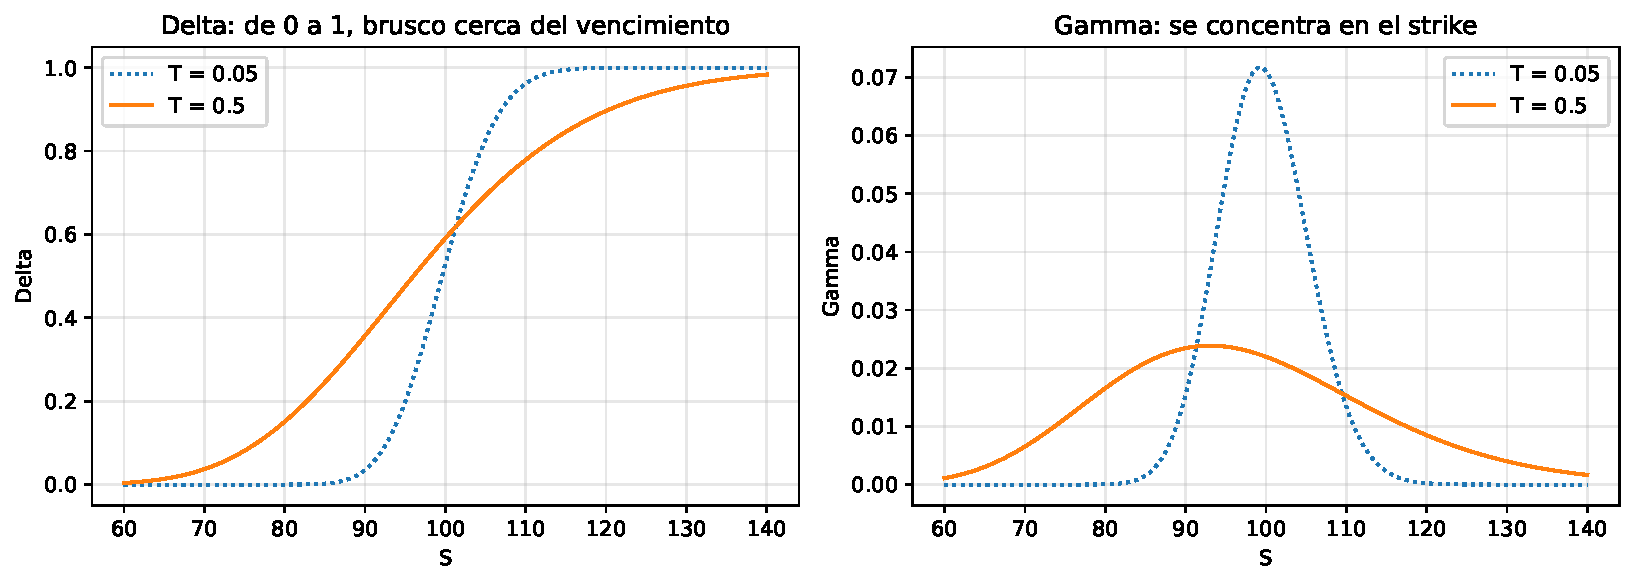
\includegraphics[keepaspectratio]{unidad4/cap18_derivados_vol_implicita_files/figure-pdf/griegas-perfil-output-1.pdf}}

El gamma concentrado alrededor del strike, y cada vez más puntiagudo al
acercarse el vencimiento, es el protagonista del próximo capítulo: es lo
que hace que cubrir una opción \textbf{cerca del vencimiento y cerca del
strike} sea un deporte de riesgo.

\begin{center}\rule{0.5\linewidth}{0.5pt}\end{center}

\chapter{Errores comunes}\label{errores-comunes-16}

\begin{tcolorbox}[enhanced jigsaw, bottomrule=.15mm, colback=white, opacitybacktitle=0.6, arc=.35mm, toprule=.15mm, opacityback=0, breakable, titlerule=0mm, left=2mm, coltitle=black, colbacktitle=quarto-callout-warning-color!10!white, colframe=quarto-callout-warning-color-frame, leftrule=.75mm, toptitle=1mm, bottomtitle=1mm, title=\textcolor{quarto-callout-warning-color}{\faExclamationTriangle}\hspace{0.5em}{Trampas frecuentes}, rightrule=.15mm]

\begin{itemize}
\tightlist
\item
  \textbf{Unidades del theta}: la derivada es ``por año''; dividí por
  365 para el decaimiento diario que se reporta en las pantallas.
\item
  \textbf{Newton sin red}: lejos del dinero, el vega es casi cero y
  Newton-Raphson diverge. Para uso robusto, combiná con bisección
  (\texttt{scipy.optimize.brentq}) que garantiza convergencia.
\item
  \textbf{Volatilidad en las unidades equivocadas}: \(\sigma\) = 0.25,
  no 25. Un factor 100 en la vol produce precios absurdos
  silenciosamente.
\item
  \textbf{Aplicar Black-Scholes a opciones americanas}: la fórmula es
  para ejercicio \emph{europeo} (solo al vencimiento). Para americanas
  con dividendos, el ejercicio temprano vale y se necesitan árboles o
  métodos numéricos.
\item
  \textbf{Paso de diferencias finitas mal elegido}: \(h\) demasiado
  grande sesga; demasiado chico amplifica el error de redondeo. Los
  valores del código (dS=0.01) son un buen punto medio para este
  problema.
\end{itemize}

\end{tcolorbox}

\begin{center}\rule{0.5\linewidth}{0.5pt}\end{center}

\chapter{Ejercicios Propuestos}\label{ejercicios-propuestos-17}

\begin{tcolorbox}[enhanced jigsaw, bottomrule=.15mm, colback=white, opacitybacktitle=0.6, arc=.35mm, toprule=.15mm, opacityback=0, breakable, titlerule=0mm, left=2mm, coltitle=black, colbacktitle=quarto-callout-important-color!10!white, colframe=quarto-callout-important-color-frame, leftrule=.75mm, toptitle=1mm, bottomtitle=1mm, title=\textcolor{quarto-callout-important-color}{\faExclamation}\hspace{0.5em}{Ejercicios}, rightrule=.15mm]

\begin{enumerate}
\def\labelenumi{\arabic{enumi}.}
\tightlist
\item
  \textbf{Griegas analíticas}: implementá el delta (\(N(d_1)\)), el
  gamma y el vega con sus fórmulas cerradas y verificá contra
  diferencias finitas con 6 decimales.
\item
  \textbf{Newton vs.~brentq}: compará \texttt{implied\_vol} con
  \texttt{scipy.optimize.brentq} en precisión y número de iteraciones,
  para strikes de 80 a 120. ¿Dónde falla Newton?
\item
  \textbf{Vol implícita de puts}: adaptá \texttt{implied\_vol} para puts
  y verificá que, por paridad, la vol implícita de una call y una put
  del mismo strike coinciden.
\item
  \textbf{Superficie de volatilidad}: extendé la sonrisa a varios
  vencimientos (1, 3, 6, 12 meses) y graficá la superficie 3D con
  \texttt{plot\_surface}.
\item
  \textbf{P\&L de un día}: para la call del capítulo, calculá la
  ganancia/pérdida aproximada si mañana \(S\) sube 2\% y la vol cae 1
  punto, usando
  \(\Delta \cdot dS + \frac{1}{2}\Gamma \cdot dS^2 + \text{Vega} \cdot d\sigma + \Theta \cdot dt\).
  Verificá repreciando con la fórmula exacta.
\end{enumerate}

\end{tcolorbox}

Podés resolver estos ejercicios acá mismo: la celda ejecuta Python
\textbf{en tu navegador}, sin instalar nada (la primera ejecución tarda
unos segundos mientras carga el entorno; los paquetes que importes se
instalan solos).

\begin{Shaded}
\begin{Highlighting}[]
\NormalTok{\#| label: practica{-}navegador}
\NormalTok{import numpy as np}
\NormalTok{from scipy.stats import norm}

\NormalTok{\# Tu solución acá...}
\end{Highlighting}
\end{Shaded}

\begin{center}\rule{0.5\linewidth}{0.5pt}\end{center}

\chapter{Referencias}\label{referencias-17}

\phantomsection\label{refs}

\chapter{Capítulo 19: Simulación de Cobertura Dinámica (Delta
Hedging)}\label{capuxedtulo-19-simulaciuxf3n-de-cobertura-dinuxe1mica-delta-hedging}

Replicar una opción operando el subyacente

El capítulo más integrador del libro: simulamos el día a día de un
trader que vendió una call y se cubre recalculando su delta y
rebalanceando acciones cada jornada. En el camino descubrimos la idea
que fundamenta Black-Scholes ---una opción se puede replicar---, medimos
el error de cobertura, entendemos por qué el gamma lo gobierna, y
estudiamos cómo la frecuencia de rebalanceo y los costos cambian el
resultado.

\hfill\break

\chapter{Introducción}\label{introducciuxf3n-16}

Imaginate que trabajás en la mesa de derivados de un banco y un cliente
te compra una call. Cobraste la prima, pero ahora tenés un problema: si
la acción sube fuerte, el payoff que vas a tener que pagar crece sin
límite. \textbf{¿Cómo dormís tranquilo?}

La respuesta es la idea más profunda de todo el pricing de derivados:
\textbf{cubrirse replicando}. Si la call tiene delta 0.57, su valor se
mueve como 0.57 acciones; entonces comprás 0.57 acciones y tu posición
combinada (call vendida + acciones) queda momentáneamente
\textbf{insensible} al precio. El problema es que el delta cambia cuando
el precio se mueve (eso es el gamma) y cuando pasa el tiempo --- así que
la cobertura hay que \textbf{rebalancearla continuamente}. De ahí el
nombre: cobertura dinámica.

Y acá la conexión conceptual con el capítulo anterior: Black y Scholes
derivaron su fórmula mostrando que esta estrategia de réplica, llevada
al límite continuo, reproduce el payoff de la opción
\textbf{exactamente}, sin importar hacia dónde vaya el mercado. El
precio de la opción \emph{es} el costo de replicarla. La simulación de
este capítulo es, en el fondo, \textbf{la demostración experimental de
Black-Scholes}.

Vamos a construirla completa, integrando todo el libro: GBM (Cap. 13),
Black-Scholes y griegas (Cap. 18), y pandas para el registro de
operaciones (Cap. 6).

\phantomsection\label{setup}
\begin{Shaded}
\begin{Highlighting}[]
\ImportTok{import}\NormalTok{ numpy }\ImportTok{as}\NormalTok{ np}
\ImportTok{import}\NormalTok{ pandas }\ImportTok{as}\NormalTok{ pd}
\ImportTok{import}\NormalTok{ matplotlib.pyplot }\ImportTok{as}\NormalTok{ plt}
\ImportTok{from}\NormalTok{ scipy.stats }\ImportTok{import}\NormalTok{ norm}

\NormalTok{rng }\OperatorTok{=}\NormalTok{ np.random.default\_rng(}\DecValTok{42}\NormalTok{)}

\CommentTok{\# El contrato que vendimos y el mercado}
\NormalTok{S0, K, T }\OperatorTok{=} \DecValTok{100}\NormalTok{, }\DecValTok{100}\NormalTok{, }\FloatTok{1.0}     \CommentTok{\# call al dinero, 1 año}
\NormalTok{r, sigma }\OperatorTok{=} \FloatTok{0.05}\NormalTok{, }\FloatTok{0.25}
\NormalTok{n\_dias }\OperatorTok{=} \DecValTok{252}
\NormalTok{dt }\OperatorTok{=}\NormalTok{ T }\OperatorTok{/}\NormalTok{ n\_dias}

\KeywordTok{def}\NormalTok{ bs\_call(S, K, T, r, sigma):}
    \CommentTok{"""Precio Black{-}Scholes de una call (maneja T=0 devolviendo el payoff)."""}
    \ControlFlowTok{if}\NormalTok{ T }\OperatorTok{\textless{}=} \DecValTok{0}\NormalTok{:}
        \ControlFlowTok{return}\NormalTok{ np.maximum(S }\OperatorTok{{-}}\NormalTok{ K, }\FloatTok{0.0}\NormalTok{)}
\NormalTok{    d1 }\OperatorTok{=}\NormalTok{ (np.log(S }\OperatorTok{/}\NormalTok{ K) }\OperatorTok{+}\NormalTok{ (r }\OperatorTok{+} \FloatTok{0.5} \OperatorTok{*}\NormalTok{ sigma}\OperatorTok{**}\DecValTok{2}\NormalTok{) }\OperatorTok{*}\NormalTok{ T) }\OperatorTok{/}\NormalTok{ (sigma }\OperatorTok{*}\NormalTok{ np.sqrt(T))}
\NormalTok{    d2 }\OperatorTok{=}\NormalTok{ d1 }\OperatorTok{{-}}\NormalTok{ sigma }\OperatorTok{*}\NormalTok{ np.sqrt(T)}
    \ControlFlowTok{return}\NormalTok{ S }\OperatorTok{*}\NormalTok{ norm.cdf(d1) }\OperatorTok{{-}}\NormalTok{ K }\OperatorTok{*}\NormalTok{ np.exp(}\OperatorTok{{-}}\NormalTok{r }\OperatorTok{*}\NormalTok{ T) }\OperatorTok{*}\NormalTok{ norm.cdf(d2)}

\KeywordTok{def}\NormalTok{ bs\_delta(S, K, T, r, sigma):}
    \CommentTok{"""Delta de la call: N(d1). En el vencimiento, escalón 0/1."""}
    \ControlFlowTok{if}\NormalTok{ T }\OperatorTok{\textless{}=} \DecValTok{0}\NormalTok{:}
        \ControlFlowTok{return} \BuiltInTok{float}\NormalTok{(S }\OperatorTok{\textgreater{}}\NormalTok{ K)}
\NormalTok{    d1 }\OperatorTok{=}\NormalTok{ (np.log(S }\OperatorTok{/}\NormalTok{ K) }\OperatorTok{+}\NormalTok{ (r }\OperatorTok{+} \FloatTok{0.5} \OperatorTok{*}\NormalTok{ sigma}\OperatorTok{**}\DecValTok{2}\NormalTok{) }\OperatorTok{*}\NormalTok{ T) }\OperatorTok{/}\NormalTok{ (sigma }\OperatorTok{*}\NormalTok{ np.sqrt(T))}
    \ControlFlowTok{return}\NormalTok{ norm.cdf(d1)}
\end{Highlighting}
\end{Shaded}

\begin{center}\rule{0.5\linewidth}{0.5pt}\end{center}

\chapter{La mecánica de un día de
trading}\label{la-mecuxe1nica-de-un-duxeda-de-trading}

La rutina diaria del trader cubierto, que vamos a codificar tal cual:

\begin{enumerate}
\def\labelenumi{\arabic{enumi}.}
\tightlist
\item
  \textbf{Amanece}: el precio se movió. Recalculás el delta de la opción
  con el precio nuevo y el tiempo restante.
\item
  \textbf{Rebalanceás}: si el delta subió de 0.55 a 0.60, comprás 0.05
  acciones más; si bajó, vendés. El cash de esas operaciones entra o
  sale de tu cuenta.
\item
  \textbf{El cash devenga interés} (o pagás por el financiamiento si
  estás en descubierto).
\item
  Al vencimiento, pagás el payoff al cliente y cerrás la posición en
  acciones.
\end{enumerate}

Si la réplica es buena, la prima cobrada al inicio + los resultados del
trading deberían cubrir \textbf{casi exactamente} el payoff. La
diferencia es el \textbf{error de cobertura}.

\phantomsection\label{simular-camino}
\begin{Shaded}
\begin{Highlighting}[]
\CommentTok{\# Un escenario de mercado: el precio evoluciona como GBM}
\NormalTok{Z }\OperatorTok{=}\NormalTok{ rng.standard\_normal(n\_dias)}
\NormalTok{S }\OperatorTok{=}\NormalTok{ np.empty(n\_dias }\OperatorTok{+} \DecValTok{1}\NormalTok{)}
\NormalTok{S[}\DecValTok{0}\NormalTok{] }\OperatorTok{=}\NormalTok{ S0}
\ControlFlowTok{for}\NormalTok{ t }\KeywordTok{in} \BuiltInTok{range}\NormalTok{(}\DecValTok{1}\NormalTok{, n\_dias }\OperatorTok{+} \DecValTok{1}\NormalTok{):}
\NormalTok{    S[t] }\OperatorTok{=}\NormalTok{ S[t}\OperatorTok{{-}}\DecValTok{1}\NormalTok{] }\OperatorTok{*}\NormalTok{ np.exp((r }\OperatorTok{{-}} \FloatTok{0.5} \OperatorTok{*}\NormalTok{ sigma}\OperatorTok{**}\DecValTok{2}\NormalTok{) }\OperatorTok{*}\NormalTok{ dt }\OperatorTok{+}\NormalTok{ sigma }\OperatorTok{*}\NormalTok{ np.sqrt(dt) }\OperatorTok{*}\NormalTok{ Z[t}\OperatorTok{{-}}\DecValTok{1}\NormalTok{])}

\BuiltInTok{print}\NormalTok{(}\SpecialStringTok{f"Precio final: $}\SpecialCharTok{\{}\NormalTok{S[}\OperatorTok{{-}}\DecValTok{1}\NormalTok{]}\SpecialCharTok{:.2f\}}\SpecialStringTok{ → la call termina "}
      \SpecialStringTok{f"}\SpecialCharTok{\{}\StringTok{\textquotesingle{}DENTRO del dinero (habrá que pagar)\textquotesingle{}} \ControlFlowTok{if}\NormalTok{ S[}\OperatorTok{{-}}\DecValTok{1}\NormalTok{] }\OperatorTok{\textgreater{}}\NormalTok{ K }\ControlFlowTok{else} \StringTok{\textquotesingle{}fuera del dinero (expira sin valor)\textquotesingle{}}\SpecialCharTok{\}}\SpecialStringTok{"}\NormalTok{)}
\end{Highlighting}
\end{Shaded}

\begin{verbatim}
Precio final: $84.10 → la call termina fuera del dinero (expira sin valor)
\end{verbatim}

\phantomsection\label{delta-hedging}
\begin{Shaded}
\begin{Highlighting}[]
\NormalTok{prima }\OperatorTok{=}\NormalTok{ bs\_call(S0, K, T, r, sigma)}

\NormalTok{registros }\OperatorTok{=}\NormalTok{ []}
\NormalTok{cash }\OperatorTok{=}\NormalTok{ prima          }\CommentTok{\# arrancamos con la prima cobrada}
\NormalTok{acciones }\OperatorTok{=} \FloatTok{0.0}        \CommentTok{\# y sin acciones}

\ControlFlowTok{for}\NormalTok{ t }\KeywordTok{in} \BuiltInTok{range}\NormalTok{(n\_dias }\OperatorTok{+} \DecValTok{1}\NormalTok{):}
\NormalTok{    tiempo\_restante }\OperatorTok{=}\NormalTok{ T }\OperatorTok{{-}}\NormalTok{ t }\OperatorTok{*}\NormalTok{ dt}
\NormalTok{    delta }\OperatorTok{=}\NormalTok{ bs\_delta(S[t], K, tiempo\_restante, r, sigma)}

    \CommentTok{\# Rebalanceo: llevamos la posición en acciones al delta de hoy}
\NormalTok{    trade }\OperatorTok{=}\NormalTok{ delta }\OperatorTok{{-}}\NormalTok{ acciones}
\NormalTok{    cash }\OperatorTok{{-}=}\NormalTok{ trade }\OperatorTok{*}\NormalTok{ S[t]          }\CommentTok{\# comprar acciones consume cash (vender lo repone)}
\NormalTok{    acciones }\OperatorTok{=}\NormalTok{ delta}

    \CommentTok{\# El cash devenga la tasa libre de riesgo hasta mañana}
    \ControlFlowTok{if}\NormalTok{ t }\OperatorTok{\textless{}}\NormalTok{ n\_dias:}
\NormalTok{        cash }\OperatorTok{*=}\NormalTok{ np.exp(r }\OperatorTok{*}\NormalTok{ dt)}

    \CommentTok{\# Mark{-}to{-}market: ¿cómo venimos vs. la opción que debemos?}
\NormalTok{    valor\_opcion }\OperatorTok{=}\NormalTok{ bs\_call(S[t], K, tiempo\_restante, r, sigma)}
\NormalTok{    valor\_cartera }\OperatorTok{=}\NormalTok{ acciones }\OperatorTok{*}\NormalTok{ S[t] }\OperatorTok{+}\NormalTok{ cash}

\NormalTok{    registros.append(\{}
        \StringTok{"dia"}\NormalTok{: t, }\StringTok{"precio"}\NormalTok{: S[t], }\StringTok{"delta"}\NormalTok{: delta, }\StringTok{"trade"}\NormalTok{: trade,}
        \StringTok{"cash"}\NormalTok{: cash, }\StringTok{"valor\_opcion"}\NormalTok{: valor\_opcion,}
        \StringTok{"valor\_cartera"}\NormalTok{: valor\_cartera,}
        \StringTok{"pnl"}\NormalTok{: valor\_cartera }\OperatorTok{{-}}\NormalTok{ valor\_opcion,}
\NormalTok{    \})}

\NormalTok{df }\OperatorTok{=}\NormalTok{ pd.DataFrame(registros)}

\NormalTok{payoff\_final }\OperatorTok{=} \BuiltInTok{max}\NormalTok{(S[}\OperatorTok{{-}}\DecValTok{1}\NormalTok{] }\OperatorTok{{-}}\NormalTok{ K, }\DecValTok{0}\NormalTok{)}
\NormalTok{error\_hedge }\OperatorTok{=}\NormalTok{ df.iloc[}\OperatorTok{{-}}\DecValTok{1}\NormalTok{][}\StringTok{"valor\_cartera"}\NormalTok{] }\OperatorTok{{-}}\NormalTok{ payoff\_final}

\BuiltInTok{print}\NormalTok{(}\SpecialStringTok{f"Prima cobrada al inicio:  $}\SpecialCharTok{\{}\NormalTok{prima}\SpecialCharTok{:8.2f\}}\SpecialStringTok{"}\NormalTok{)}
\BuiltInTok{print}\NormalTok{(}\SpecialStringTok{f"Payoff a pagar al cliente:$}\SpecialCharTok{\{}\NormalTok{payoff\_final}\SpecialCharTok{:8.2f\}}\SpecialStringTok{"}\NormalTok{)}
\BuiltInTok{print}\NormalTok{(}\SpecialStringTok{f"Valor final de la réplica:$}\SpecialCharTok{\{}\NormalTok{df}\SpecialCharTok{.}\NormalTok{iloc[}\OperatorTok{{-}}\DecValTok{1}\NormalTok{][}\StringTok{\textquotesingle{}valor\_cartera\textquotesingle{}}\NormalTok{]}\SpecialCharTok{:8.2f\}}\SpecialStringTok{"}\NormalTok{)}
\BuiltInTok{print}\NormalTok{(}\SpecialStringTok{f"Error de cobertura:       $}\SpecialCharTok{\{}\NormalTok{error\_hedge}\SpecialCharTok{:8.2f\}}\SpecialStringTok{  "}
      \SpecialStringTok{f"(}\SpecialCharTok{\{}\NormalTok{error\_hedge }\OperatorTok{/}\NormalTok{ prima}\SpecialCharTok{:+.1\%\}}\SpecialStringTok{ de la prima)"}\NormalTok{)}
\end{Highlighting}
\end{Shaded}

\begin{verbatim}
Prima cobrada al inicio:  $   12.34
Payoff a pagar al cliente:$    0.00
Valor final de la réplica:$    0.91
Error de cobertura:       $    0.91  (+7.4% de la prima)
\end{verbatim}

Leé el resultado con perspectiva: el precio se movió durante un año
entero ---quizás terminó 20\% arriba o abajo--- y sin embargo el trader
cubierto termina con un error de \textbf{centavos por cada 100 de
prima}. No adivinó el mercado ni le hizo falta: la réplica transformó
una posición especulativa en un negocio de fabricación. El banco
``fabrica'' la opción comprando y vendiendo el subyacente, y su ganancia
es el margen sobre el costo de fabricación --- no una apuesta
direccional.

\begin{Shaded}
\begin{Highlighting}[]
\NormalTok{fig, axes }\OperatorTok{=}\NormalTok{ plt.subplots(}\DecValTok{2}\NormalTok{, }\DecValTok{2}\NormalTok{, figsize}\OperatorTok{=}\NormalTok{(}\DecValTok{12}\NormalTok{, }\DecValTok{8}\NormalTok{))}

\NormalTok{ax }\OperatorTok{=}\NormalTok{ axes[}\DecValTok{0}\NormalTok{, }\DecValTok{0}\NormalTok{]}
\NormalTok{ax.plot(df[}\StringTok{"dia"}\NormalTok{], df[}\StringTok{"precio"}\NormalTok{], linewidth}\OperatorTok{=}\FloatTok{1.2}\NormalTok{)}
\NormalTok{ax.axhline(K, color}\OperatorTok{=}\StringTok{"red"}\NormalTok{, linestyle}\OperatorTok{=}\StringTok{"{-}{-}"}\NormalTok{, alpha}\OperatorTok{=}\FloatTok{0.6}\NormalTok{, label}\OperatorTok{=}\SpecialStringTok{f"Strike K=}\SpecialCharTok{\{}\NormalTok{K}\SpecialCharTok{\}}\SpecialStringTok{"}\NormalTok{)}
\NormalTok{ax.set\_title(}\StringTok{"El escenario: precio del subyacente"}\NormalTok{)}
\NormalTok{ax.set\_ylabel(}\StringTok{"Precio ($)"}\NormalTok{)}
\NormalTok{ax.legend()}
\NormalTok{ax.grid(}\VariableTok{True}\NormalTok{, alpha}\OperatorTok{=}\FloatTok{0.3}\NormalTok{)}

\NormalTok{ax }\OperatorTok{=}\NormalTok{ axes[}\DecValTok{0}\NormalTok{, }\DecValTok{1}\NormalTok{]}
\NormalTok{ax.plot(df[}\StringTok{"dia"}\NormalTok{], df[}\StringTok{"delta"}\NormalTok{], color}\OperatorTok{=}\StringTok{"green"}\NormalTok{, linewidth}\OperatorTok{=}\FloatTok{1.2}\NormalTok{)}
\NormalTok{ax.set\_title(}\StringTok{"La posición: delta = acciones en cartera"}\NormalTok{)}
\NormalTok{ax.set\_ylabel(}\StringTok{"Delta"}\NormalTok{)}
\NormalTok{ax.grid(}\VariableTok{True}\NormalTok{, alpha}\OperatorTok{=}\FloatTok{0.3}\NormalTok{)}

\NormalTok{ax }\OperatorTok{=}\NormalTok{ axes[}\DecValTok{1}\NormalTok{, }\DecValTok{0}\NormalTok{]}
\NormalTok{ax.plot(df[}\StringTok{"dia"}\NormalTok{], df[}\StringTok{"valor\_cartera"}\NormalTok{], label}\OperatorTok{=}\StringTok{"Cartera replicante"}\NormalTok{, linewidth}\OperatorTok{=}\FloatTok{1.2}\NormalTok{)}
\NormalTok{ax.plot(df[}\StringTok{"dia"}\NormalTok{], df[}\StringTok{"valor\_opcion"}\NormalTok{], }\StringTok{"{-}{-}"}\NormalTok{, label}\OperatorTok{=}\StringTok{"Valor de la opción"}\NormalTok{, linewidth}\OperatorTok{=}\FloatTok{1.2}\NormalTok{)}
\NormalTok{ax.set\_title(}\StringTok{"La réplica en acción: dos curvas casi idénticas"}\NormalTok{)}
\NormalTok{ax.set\_xlabel(}\StringTok{"Día"}\NormalTok{)}
\NormalTok{ax.set\_ylabel(}\StringTok{"Valor ($)"}\NormalTok{)}
\NormalTok{ax.legend()}
\NormalTok{ax.grid(}\VariableTok{True}\NormalTok{, alpha}\OperatorTok{=}\FloatTok{0.3}\NormalTok{)}

\NormalTok{ax }\OperatorTok{=}\NormalTok{ axes[}\DecValTok{1}\NormalTok{, }\DecValTok{1}\NormalTok{]}
\NormalTok{ax.bar(df[}\StringTok{"dia"}\NormalTok{], df[}\StringTok{"trade"}\NormalTok{], color}\OperatorTok{=}\StringTok{"steelblue"}\NormalTok{, alpha}\OperatorTok{=}\FloatTok{0.7}\NormalTok{, width}\OperatorTok{=}\FloatTok{1.5}\NormalTok{)}
\NormalTok{ax.set\_title(}\StringTok{"Los rebalanceos diarios"}\NormalTok{)}
\NormalTok{ax.set\_xlabel(}\StringTok{"Día"}\NormalTok{)}
\NormalTok{ax.set\_ylabel(}\StringTok{"Acciones operadas"}\NormalTok{)}
\NormalTok{ax.grid(}\VariableTok{True}\NormalTok{, alpha}\OperatorTok{=}\FloatTok{0.3}\NormalTok{)}

\NormalTok{plt.tight\_layout()}
\NormalTok{plt.show()}
\end{Highlighting}
\end{Shaded}

\pandocbounded{\includegraphics[keepaspectratio]{unidad4/cap19_delta_hedging_files/figure-pdf/plots-output-1.pdf}}

Fijate dos cosas en los gráficos. Primero, el panel inferior izquierdo:
la cartera replicante \textbf{persigue al valor de la opción} durante
todo el año --- esa es la réplica funcionando. Segundo, el panel del
delta comparado con el del precio: cuando el precio cruza el strike, el
delta se mueve rápido y los rebalanceos se agrandan. Ahí gobierna el
\textbf{gamma}.

\begin{tcolorbox}[enhanced jigsaw, bottomrule=.15mm, colback=white, opacitybacktitle=0.6, arc=.35mm, toprule=.15mm, opacityback=0, breakable, titlerule=0mm, left=2mm, coltitle=black, colbacktitle=quarto-callout-tip-color!10!white, colframe=quarto-callout-tip-color-frame, leftrule=.75mm, toptitle=1mm, bottomtitle=1mm, title=\textcolor{quarto-callout-tip-color}{\faLightbulb}\hspace{0.5em}{Comprar caro y vender barato, por diseño}, rightrule=.15mm]

Observá el patrón de los trades: cuando el precio \textbf{sube}, el
delta sube y el trader \textbf{compra}; cuando \textbf{baja},
\textbf{vende}. El cubridor de una opción vendida compra en las subas y
vende en las bajas --- sistemáticamente pierde en cada ida y vuelta. Ese
costo acumulado no es un defecto: \textbf{es exactamente el valor
temporal de la opción} que cobró como prima. Si la volatilidad realizada
termina siendo la que cotizó (\(\sigma\)), prima y costo de cobertura se
cancelan. Si el mercado se mueve \emph{más} que lo cotizado, el cubridor
pierde; si se mueve \emph{menos}, gana. Vender opciones cubiertas es, en
el fondo, \textbf{vender volatilidad}.

\end{tcolorbox}

\begin{center}\rule{0.5\linewidth}{0.5pt}\end{center}

\chapter{El error de cobertura: de dónde viene y cómo se
achica}\label{el-error-de-cobertura-de-duxf3nde-viene-y-cuxf3mo-se-achica}

En el mundo ideal de Black-Scholes el rebalanceo es \emph{continuo} y el
error es cero. Nosotros rebalanceamos una vez por día, y entre
rebalanceo y rebalanceo el delta queda desactualizado. ¿Cuánto cuesta
esa discretización? La respuesta la da el \textbf{gamma}: entre dos
rebalanceos, el error de la aproximación lineal es
\(\tfrac{1}{2}\Gamma (\Delta S)^2\) --- cuadrático en el movimiento del
precio.

La teoría predice algo verificable: el error de cobertura tiene media
\textasciitilde0 y su desvío \textbf{cae como \(1/\sqrt{n}\)} con la
frecuencia de rebalanceo. Comprobémoslo con un experimento masivo:

\begin{Shaded}
\begin{Highlighting}[]
\KeywordTok{def}\NormalTok{ error\_hedging(n\_rebalanceos, n\_sims, rng):}
    \CommentTok{"""Distribución del error de cobertura para una frecuencia dada."""}
\NormalTok{    dt\_h }\OperatorTok{=}\NormalTok{ T }\OperatorTok{/}\NormalTok{ n\_rebalanceos}
\NormalTok{    errores }\OperatorTok{=}\NormalTok{ np.empty(n\_sims)}

    \ControlFlowTok{for}\NormalTok{ i }\KeywordTok{in} \BuiltInTok{range}\NormalTok{(n\_sims):}
\NormalTok{        Z }\OperatorTok{=}\NormalTok{ rng.standard\_normal(n\_rebalanceos)}
\NormalTok{        S\_t, cash, acc }\OperatorTok{=}\NormalTok{ S0, prima, }\FloatTok{0.0}
        \ControlFlowTok{for}\NormalTok{ t }\KeywordTok{in} \BuiltInTok{range}\NormalTok{(n\_rebalanceos):}
\NormalTok{            delta }\OperatorTok{=}\NormalTok{ bs\_delta(S\_t, K, T }\OperatorTok{{-}}\NormalTok{ t }\OperatorTok{*}\NormalTok{ dt\_h, r, sigma)}
\NormalTok{            cash }\OperatorTok{{-}=}\NormalTok{ (delta }\OperatorTok{{-}}\NormalTok{ acc) }\OperatorTok{*}\NormalTok{ S\_t}
\NormalTok{            acc }\OperatorTok{=}\NormalTok{ delta}
\NormalTok{            cash }\OperatorTok{*=}\NormalTok{ np.exp(r }\OperatorTok{*}\NormalTok{ dt\_h)}
\NormalTok{            S\_t }\OperatorTok{*=}\NormalTok{ np.exp((r }\OperatorTok{{-}} \FloatTok{0.5} \OperatorTok{*}\NormalTok{ sigma}\OperatorTok{**}\DecValTok{2}\NormalTok{) }\OperatorTok{*}\NormalTok{ dt\_h }\OperatorTok{+}\NormalTok{ sigma }\OperatorTok{*}\NormalTok{ np.sqrt(dt\_h) }\OperatorTok{*}\NormalTok{ Z[t])}
\NormalTok{        errores[i] }\OperatorTok{=}\NormalTok{ acc }\OperatorTok{*}\NormalTok{ S\_t }\OperatorTok{+}\NormalTok{ cash }\OperatorTok{{-}} \BuiltInTok{max}\NormalTok{(S\_t }\OperatorTok{{-}}\NormalTok{ K, }\DecValTok{0}\NormalTok{)}
    \ControlFlowTok{return}\NormalTok{ errores}

\NormalTok{frecuencias }\OperatorTok{=}\NormalTok{ \{}\StringTok{"Mensual (12)"}\NormalTok{: }\DecValTok{12}\NormalTok{, }\StringTok{"Semanal (52)"}\NormalTok{: }\DecValTok{52}\NormalTok{, }\StringTok{"Diaria (252)"}\NormalTok{: }\DecValTok{252}\NormalTok{\}}
\NormalTok{resultados }\OperatorTok{=}\NormalTok{ \{nombre: error\_hedging(n, }\DecValTok{400}\NormalTok{, np.random.default\_rng(}\DecValTok{7}\NormalTok{))}
              \ControlFlowTok{for}\NormalTok{ nombre, n }\KeywordTok{in}\NormalTok{ frecuencias.items()\}}

\BuiltInTok{print}\NormalTok{(}\SpecialStringTok{f"}\SpecialCharTok{\{}\StringTok{\textquotesingle{}Rebalanceo\textquotesingle{}}\SpecialCharTok{:\textless{}16\}\{}\StringTok{\textquotesingle{}Error medio\textquotesingle{}}\SpecialCharTok{:\textgreater{}12\}\{}\StringTok{\textquotesingle{}Desvío\textquotesingle{}}\SpecialCharTok{:\textgreater{}10\}}\SpecialStringTok{"}\NormalTok{)}
\ControlFlowTok{for}\NormalTok{ nombre, err }\KeywordTok{in}\NormalTok{ resultados.items():}
    \BuiltInTok{print}\NormalTok{(}\SpecialStringTok{f"}\SpecialCharTok{\{}\NormalTok{nombre}\SpecialCharTok{:\textless{}16\}\{}\NormalTok{err}\SpecialCharTok{.}\NormalTok{mean()}\SpecialCharTok{:\textgreater{}12.3f\}\{}\NormalTok{err}\SpecialCharTok{.}\NormalTok{std()}\SpecialCharTok{:\textgreater{}10.3f\}}\SpecialStringTok{"}\NormalTok{)}

\NormalTok{fig, ax }\OperatorTok{=}\NormalTok{ plt.subplots(figsize}\OperatorTok{=}\NormalTok{(}\DecValTok{9}\NormalTok{, }\FloatTok{4.5}\NormalTok{))}
\ControlFlowTok{for}\NormalTok{ nombre, err }\KeywordTok{in}\NormalTok{ resultados.items():}
\NormalTok{    ax.hist(err, bins}\OperatorTok{=}\DecValTok{40}\NormalTok{, alpha}\OperatorTok{=}\FloatTok{0.55}\NormalTok{, label}\OperatorTok{=}\NormalTok{nombre, density}\OperatorTok{=}\VariableTok{True}\NormalTok{)}
\NormalTok{ax.axvline(}\DecValTok{0}\NormalTok{, color}\OperatorTok{=}\StringTok{"black"}\NormalTok{, alpha}\OperatorTok{=}\FloatTok{0.4}\NormalTok{)}
\NormalTok{ax.set\_xlabel(}\StringTok{"Error de cobertura ($)"}\NormalTok{)}
\NormalTok{ax.set\_ylabel(}\StringTok{"Densidad"}\NormalTok{)}
\NormalTok{ax.set\_title(}\StringTok{"Rebalancear más seguido angosta la distribución del error"}\NormalTok{)}
\NormalTok{ax.legend()}
\NormalTok{ax.grid(}\VariableTok{True}\NormalTok{, alpha}\OperatorTok{=}\FloatTok{0.3}\NormalTok{)}
\NormalTok{plt.tight\_layout()}
\NormalTok{plt.show()}
\end{Highlighting}
\end{Shaded}

\begin{verbatim}
Rebalanceo       Error medio    Desvío
Mensual (12)           0.085     2.181
Semanal (52)           0.079     1.130
Diaria (252)          -0.009     0.567
\end{verbatim}

\pandocbounded{\includegraphics[keepaspectratio]{unidad4/cap19_delta_hedging_files/figure-pdf/frecuencia-output-2.pdf}}

La media es \textasciitilde0 en todos los casos (la cobertura no está
sesgada) y el desvío se achica con la raíz de la frecuencia: de mensual
a diario hay un factor \(\sqrt{252/12} \approx 4.6\). En el límite
continuo, el error desaparece --- \textbf{esa es la demostración
experimental del argumento de Black-Scholes}.

\section{El freno del mundo real: costos de
transacción}\label{el-freno-del-mundo-real-costos-de-transacciuxf3n}

¿Entonces por qué no rebalancear cada minuto? Porque cada operación
\textbf{cuesta} (comisiones, spread). Más frecuencia = menos error de
gamma pero más costos: hay un punto óptimo intermedio, y encontrarlo es
un problema clásico de la microestructura de la cobertura.

\phantomsection\label{costos}
\begin{Shaded}
\begin{Highlighting}[]
\KeywordTok{def}\NormalTok{ error\_con\_costos(n\_rebalanceos, costo\_bps, n\_sims, rng):}
\NormalTok{    dt\_h }\OperatorTok{=}\NormalTok{ T }\OperatorTok{/}\NormalTok{ n\_rebalanceos}
\NormalTok{    errores }\OperatorTok{=}\NormalTok{ np.empty(n\_sims)}
    \ControlFlowTok{for}\NormalTok{ i }\KeywordTok{in} \BuiltInTok{range}\NormalTok{(n\_sims):}
\NormalTok{        Z }\OperatorTok{=}\NormalTok{ rng.standard\_normal(n\_rebalanceos)}
\NormalTok{        S\_t, cash, acc }\OperatorTok{=}\NormalTok{ S0, prima, }\FloatTok{0.0}
        \ControlFlowTok{for}\NormalTok{ t }\KeywordTok{in} \BuiltInTok{range}\NormalTok{(n\_rebalanceos):}
\NormalTok{            delta }\OperatorTok{=}\NormalTok{ bs\_delta(S\_t, K, T }\OperatorTok{{-}}\NormalTok{ t }\OperatorTok{*}\NormalTok{ dt\_h, r, sigma)}
\NormalTok{            trade }\OperatorTok{=}\NormalTok{ delta }\OperatorTok{{-}}\NormalTok{ acc}
\NormalTok{            cash }\OperatorTok{{-}=}\NormalTok{ trade }\OperatorTok{*}\NormalTok{ S\_t }\OperatorTok{+} \BuiltInTok{abs}\NormalTok{(trade) }\OperatorTok{*}\NormalTok{ S\_t }\OperatorTok{*}\NormalTok{ costo\_bps }\OperatorTok{/} \FloatTok{1e4}  \CommentTok{\# costo proporcional}
\NormalTok{            acc }\OperatorTok{=}\NormalTok{ delta}
\NormalTok{            cash }\OperatorTok{*=}\NormalTok{ np.exp(r }\OperatorTok{*}\NormalTok{ dt\_h)}
\NormalTok{            S\_t }\OperatorTok{*=}\NormalTok{ np.exp((r }\OperatorTok{{-}} \FloatTok{0.5} \OperatorTok{*}\NormalTok{ sigma}\OperatorTok{**}\DecValTok{2}\NormalTok{) }\OperatorTok{*}\NormalTok{ dt\_h }\OperatorTok{+}\NormalTok{ sigma }\OperatorTok{*}\NormalTok{ np.sqrt(dt\_h) }\OperatorTok{*}\NormalTok{ Z[t])}
\NormalTok{        errores[i] }\OperatorTok{=}\NormalTok{ acc }\OperatorTok{*}\NormalTok{ S\_t }\OperatorTok{+}\NormalTok{ cash }\OperatorTok{{-}} \BuiltInTok{max}\NormalTok{(S\_t }\OperatorTok{{-}}\NormalTok{ K, }\DecValTok{0}\NormalTok{)}
    \ControlFlowTok{return}\NormalTok{ errores}

\BuiltInTok{print}\NormalTok{(}\SpecialStringTok{f"Con costos de 5 puntos básicos por operación:"}\NormalTok{)}
\BuiltInTok{print}\NormalTok{(}\SpecialStringTok{f"}\SpecialCharTok{\{}\StringTok{\textquotesingle{}Rebalanceo\textquotesingle{}}\SpecialCharTok{:\textless{}16\}\{}\StringTok{\textquotesingle{}Error medio\textquotesingle{}}\SpecialCharTok{:\textgreater{}12\}\{}\StringTok{\textquotesingle{}Desvío\textquotesingle{}}\SpecialCharTok{:\textgreater{}10\}}\SpecialStringTok{"}\NormalTok{)}
\ControlFlowTok{for}\NormalTok{ nombre, n }\KeywordTok{in}\NormalTok{ frecuencias.items():}
\NormalTok{    err }\OperatorTok{=}\NormalTok{ error\_con\_costos(n, costo\_bps}\OperatorTok{=}\DecValTok{5}\NormalTok{, n\_sims}\OperatorTok{=}\DecValTok{400}\NormalTok{, rng}\OperatorTok{=}\NormalTok{np.random.default\_rng(}\DecValTok{7}\NormalTok{))}
    \BuiltInTok{print}\NormalTok{(}\SpecialStringTok{f"}\SpecialCharTok{\{}\NormalTok{nombre}\SpecialCharTok{:\textless{}16\}\{}\NormalTok{err}\SpecialCharTok{.}\NormalTok{mean()}\SpecialCharTok{:\textgreater{}12.3f\}\{}\NormalTok{err}\SpecialCharTok{.}\NormalTok{std()}\SpecialCharTok{:\textgreater{}10.3f\}}\SpecialStringTok{"}\NormalTok{)}
\end{Highlighting}
\end{Shaded}

\begin{verbatim}
Con costos de 5 puntos básicos por operación:
Rebalanceo       Error medio    Desvío
Mensual (12)           0.002     2.186
Semanal (52)          -0.064     1.132
Diaria (252)          -0.289     0.588
\end{verbatim}

Ahora el error medio es \textbf{negativo y empeora con la frecuencia}:
los costos son un peaje que se paga en cada rebalanceo. El trader real
equilibra: rebalancea por bandas (``solo si el delta se desvió más de
X''), usa el gamma para decidir cuándo vale la pena, y cotiza la opción
con un margen que cubra este peaje.

\begin{center}\rule{0.5\linewidth}{0.5pt}\end{center}

\chapter{Cuando el gamma muerde: cerca del strike, cerca del
vencimiento}\label{cuando-el-gamma-muerde-cerca-del-strike-cerca-del-vencimiento}

El talón de Aquiles de la cobertura delta es la zona donde el gamma
explota: \textbf{strike cercano y poco tiempo restante} (el pico
puntiagudo del capítulo anterior). Ahí el delta salta de casi-0 a casi-1
con movimientos chicos del precio, y ninguna frecuencia razonable de
rebalanceo alcanza.

\begin{Shaded}
\begin{Highlighting}[]
\CommentTok{\# Un escenario malicioso: el precio termina oscilando alrededor del strike}
\NormalTok{dias\_final }\OperatorTok{=} \DecValTok{20}
\NormalTok{S\_pin }\OperatorTok{=}\NormalTok{ np.concatenate([}
\NormalTok{    np.linspace(}\DecValTok{100}\NormalTok{, }\FloatTok{99.5}\NormalTok{, n\_dias }\OperatorTok{+} \DecValTok{1} \OperatorTok{{-}}\NormalTok{ dias\_final),          }\CommentTok{\# tranquilo hasta el final}
    \DecValTok{100} \OperatorTok{+} \FloatTok{1.5} \OperatorTok{*}\NormalTok{ np.sin(np.linspace(}\DecValTok{0}\NormalTok{, }\DecValTok{6} \OperatorTok{*}\NormalTok{ np.pi, dias\_final)) }\CommentTok{\# y baila sobre el strike}
\NormalTok{])}

\NormalTok{deltas\_pin }\OperatorTok{=}\NormalTok{ [bs\_delta(S\_pin[t], K, }\BuiltInTok{max}\NormalTok{(T }\OperatorTok{{-}}\NormalTok{ t }\OperatorTok{*}\NormalTok{ dt, }\FloatTok{1e{-}9}\NormalTok{), r, sigma)}
              \ControlFlowTok{for}\NormalTok{ t }\KeywordTok{in} \BuiltInTok{range}\NormalTok{(n\_dias }\OperatorTok{+} \DecValTok{1}\NormalTok{)]}

\NormalTok{fig, ax }\OperatorTok{=}\NormalTok{ plt.subplots(figsize}\OperatorTok{=}\NormalTok{(}\DecValTok{9}\NormalTok{, }\DecValTok{4}\NormalTok{))}
\NormalTok{ax2 }\OperatorTok{=}\NormalTok{ ax.twinx()}
\NormalTok{ax.plot(S\_pin[}\OperatorTok{{-}}\DecValTok{40}\NormalTok{:], color}\OperatorTok{=}\StringTok{"steelblue"}\NormalTok{, label}\OperatorTok{=}\StringTok{"Precio"}\NormalTok{)}
\NormalTok{ax.axhline(K, color}\OperatorTok{=}\StringTok{"red"}\NormalTok{, linestyle}\OperatorTok{=}\StringTok{"{-}{-}"}\NormalTok{, alpha}\OperatorTok{=}\FloatTok{0.5}\NormalTok{)}
\NormalTok{ax2.plot(deltas\_pin[}\OperatorTok{{-}}\DecValTok{40}\NormalTok{:], color}\OperatorTok{=}\StringTok{"darkorange"}\NormalTok{, label}\OperatorTok{=}\StringTok{"Delta"}\NormalTok{)}
\NormalTok{ax.set\_xlabel(}\StringTok{"Últimos 40 días"}\NormalTok{)}
\NormalTok{ax.set\_ylabel(}\StringTok{"Precio ($)"}\NormalTok{, color}\OperatorTok{=}\StringTok{"steelblue"}\NormalTok{)}
\NormalTok{ax2.set\_ylabel(}\StringTok{"Delta"}\NormalTok{, color}\OperatorTok{=}\StringTok{"darkorange"}\NormalTok{)}
\NormalTok{ax.set\_title(}\StringTok{"Pin risk: el delta se vuelve loco cuando el precio baila sobre el strike"}\NormalTok{)}
\NormalTok{plt.tight\_layout()}
\NormalTok{plt.show()}
\end{Highlighting}
\end{Shaded}

\pandocbounded{\includegraphics[keepaspectratio]{unidad4/cap19_delta_hedging_files/figure-pdf/pin-risk-output-1.pdf}}

En esos últimos días el trader compra arriba y vende abajo una y otra
vez, sangrando en cada vuelta --- el famoso \textbf{pin risk}. La
respuesta profesional es cubrir también la curvatura: el
\textbf{delta-gamma hedging} agrega \emph{otra opción} a la cartera para
neutralizar el gamma (las acciones solas no pueden: su gamma es cero).
Queda como ejercicio, y es la puerta de entrada a la gestión de books de
opciones reales.

\begin{center}\rule{0.5\linewidth}{0.5pt}\end{center}

\chapter{Errores comunes}\label{errores-comunes-17}

\begin{tcolorbox}[enhanced jigsaw, bottomrule=.15mm, colback=white, opacitybacktitle=0.6, arc=.35mm, toprule=.15mm, opacityback=0, breakable, titlerule=0mm, left=2mm, coltitle=black, colbacktitle=quarto-callout-warning-color!10!white, colframe=quarto-callout-warning-color-frame, leftrule=.75mm, toptitle=1mm, bottomtitle=1mm, title=\textcolor{quarto-callout-warning-color}{\faExclamationTriangle}\hspace{0.5em}{Trampas frecuentes}, rightrule=.15mm]

\begin{itemize}
\tightlist
\item
  \textbf{Olvidar el interés del cash}: en horizontes largos, el carry
  del cash es parte material del resultado; omitirlo sesga el error de
  cobertura.
\item
  \textbf{Rebalancear con el delta de ayer}: el delta debe calcularse
  con el precio y el tiempo \emph{de hoy}, antes de operar. Desfasar un
  día introduce un error sistemático.
\item
  \textbf{Confundir el P\&L del hedge con ganancia de trading}: el
  objetivo del cubridor es error \textasciitilde0; un P\&L grande (a
  favor o en contra) significa que la cobertura falló o que la vol
  realizada difirió de la cotizada.
\item
  \textbf{Ignorar el caso T→0 en las funciones}: \texttt{bs\_delta} con
  \texttt{T=0} divide por cero si no se maneja aparte; en el vencimiento
  el delta es un escalón.
\item
  \textbf{Simular con drift μ para valuar}: la réplica funciona con
  cualquier drift (esa es la magia), pero el mark-to-market usa el
  precio Black-Scholes, que vive en el mundo neutral al riesgo.
\end{itemize}

\end{tcolorbox}

\begin{center}\rule{0.5\linewidth}{0.5pt}\end{center}

\chapter{Ejercicios Propuestos}\label{ejercicios-propuestos-18}

\begin{tcolorbox}[enhanced jigsaw, bottomrule=.15mm, colback=white, opacitybacktitle=0.6, arc=.35mm, toprule=.15mm, opacityback=0, breakable, titlerule=0mm, left=2mm, coltitle=black, colbacktitle=quarto-callout-important-color!10!white, colframe=quarto-callout-important-color-frame, leftrule=.75mm, toptitle=1mm, bottomtitle=1mm, title=\textcolor{quarto-callout-important-color}{\faExclamation}\hspace{0.5em}{Ejercicios}, rightrule=.15mm]

\begin{enumerate}
\def\labelenumi{\arabic{enumi}.}
\tightlist
\item
  \textbf{Vol realizada vs.~cotizada}: simulá el mercado con
  \(\sigma_{real} = 30\%\) pero cubrí usando \(\sigma = 25\%\) en las
  fórmulas. ¿El error medio sigue siendo cero? ¿Quién gana, el comprador
  o el vendedor de la opción?
\item
  \textbf{Bandas de rebalanceo}: implementá la regla ``rebalancear solo
  si \(|\delta_{hoy} - \text{acciones}| > 0.05\)'' y comparala con el
  rebalanceo diario en error y en número de operaciones (con costos de 5
  bps).
\item
  \textbf{Delta-gamma hedging}: agregá una segunda call (strike 110) a
  la cartera para anular el gamma además del delta, y verificá que el
  error en el escenario de pin risk se reduce.
\item
  \textbf{Put vendida}: repetí la simulación completa para una put.
  ¿Cambia el signo de los rebalanceos? ¿Y la exposición al gamma?
\item
  \textbf{Salto sorpresa}: introducí un salto de −10\% en un día
  aleatorio del escenario (Capítulo 14) y medí el error de cobertura.
  ¿Por qué el delta hedging no puede protegerte de un salto?
\end{enumerate}

\end{tcolorbox}

Podés resolver estos ejercicios acá mismo: la celda ejecuta Python
\textbf{en tu navegador}, sin instalar nada (la primera ejecución tarda
unos segundos mientras carga el entorno; los paquetes que importes se
instalan solos).

\begin{Shaded}
\begin{Highlighting}[]
\NormalTok{\#| label: practica{-}navegador}
\NormalTok{import numpy as np}
\NormalTok{from scipy.stats import norm}

\NormalTok{\# Tu solución acá...}
\end{Highlighting}
\end{Shaded}

\begin{center}\rule{0.5\linewidth}{0.5pt}\end{center}

\chapter{Referencias}\label{referencias-18}

\phantomsection\label{refs}

\chapter{Capítulo 20: Modelos de Volatilidad
Estocástica}\label{capuxedtulo-20-modelos-de-volatilidad-estocuxe1stica}

Heston y SABR: cuando la volatilidad tiene vida propia

Black-Scholes trata a la volatilidad como una constante; el mercado la
cotiza distinta para cada strike y cada plazo. La salida es promover a
la volatilidad a proceso estocástico: en Heston, la varianza sigue su
propia dinámica con reversión a la media y correlación negativa con el
precio; en SABR, la industria encontró su lenguaje estándar para
interpolar sonrisas. Simulamos ambos, vemos cómo generan la sonrisa que
Black-Scholes no puede producir, y cerramos el arco completo del libro.

\hfill\break

\chapter{Introducción}\label{introducciuxf3n-17}

Cerramos el libro atacando la última gran mentira piadosa de
Black-Scholes. En el Capítulo 18 vimos la evidencia: la \textbf{sonrisa
de volatilidad}. Si la volatilidad fuera constante como supone el
modelo, la vol implícita sería la misma en todos los strikes --- y no lo
es, en ningún mercado de opciones del planeta.

En el Capítulo 14 arreglamos una parte del problema agregando
\textbf{saltos} al precio. Pero hay otro hecho estilizado que los saltos
solos no explican: la volatilidad \textbf{cambia en el tiempo, y de
manera persistente}. Hay semanas tranquilas y meses de pánico; la
volatilidad se agrupa en rachas (\emph{volatility clustering}), tiende a
volver a un nivel normal cuando se dispara, y ---el detalle crucial---
\textbf{sube cuando el mercado cae}.

La respuesta natural: si la volatilidad se comporta como un proceso
aleatorio\ldots{} \textbf{modelémosla como un proceso aleatorio}. Eso
son los modelos de volatilidad estocástica: dos procesos acoplados, uno
para el precio y otro para su volatilidad.

\phantomsection\label{setup}
\begin{Shaded}
\begin{Highlighting}[]
\ImportTok{import}\NormalTok{ numpy }\ImportTok{as}\NormalTok{ np}
\ImportTok{import}\NormalTok{ matplotlib.pyplot }\ImportTok{as}\NormalTok{ plt}
\ImportTok{from}\NormalTok{ scipy }\ImportTok{import}\NormalTok{ stats}
\ImportTok{from}\NormalTok{ scipy.stats }\ImportTok{import}\NormalTok{ norm}

\NormalTok{rng }\OperatorTok{=}\NormalTok{ np.random.default\_rng(}\DecValTok{42}\NormalTok{)}
\end{Highlighting}
\end{Shaded}

\begin{center}\rule{0.5\linewidth}{0.5pt}\end{center}

\chapter{La evidencia: la volatilidad no se queda
quieta}\label{la-evidencia-la-volatilidad-no-se-queda-quieta}

Antes de los modelos, los hechos. Tres rasgos empíricos que cualquier
serie financiera larga exhibe:

\begin{enumerate}
\def\labelenumi{\arabic{enumi}.}
\tightlist
\item
  \textbf{Clustering}: los días agitados vienen en rachas; la
  volatilidad de mañana se parece a la de hoy.
\item
  \textbf{Reversión a la media}: los picos de pánico (VIX en 80) no
  duran; la vol vuelve a su zona normal.
\item
  \textbf{Efecto apalancamiento} (\emph{leverage effect}): las caídas
  del precio vienen acompañadas de subas de volatilidad --- la
  correlación entre retornos y cambios de vol es \textbf{negativa}.
\end{enumerate}

\begin{Shaded}
\begin{Highlighting}[]
\CommentTok{\# Ilustración con datos simulados de un proceso con clustering (GARCH{-}like)}
\NormalTok{n }\OperatorTok{=} \DecValTok{1500}
\NormalTok{vol }\OperatorTok{=}\NormalTok{ np.empty(n)}\OperatorTok{;}\NormalTok{ vol[}\DecValTok{0}\NormalTok{] }\OperatorTok{=} \FloatTok{0.015}
\NormalTok{ret }\OperatorTok{=}\NormalTok{ np.empty(n)}
\ControlFlowTok{for}\NormalTok{ t }\KeywordTok{in} \BuiltInTok{range}\NormalTok{(}\DecValTok{1}\NormalTok{, n):}
    \CommentTok{\# la varianza de hoy hereda de ayer y reacciona al shock de ayer}
\NormalTok{    vol[t] }\OperatorTok{=}\NormalTok{ np.sqrt(}\FloatTok{0.02} \OperatorTok{*} \FloatTok{0.015}\OperatorTok{**}\DecValTok{2} \OperatorTok{+} \FloatTok{0.90} \OperatorTok{*}\NormalTok{ vol[t}\OperatorTok{{-}}\DecValTok{1}\NormalTok{]}\OperatorTok{**}\DecValTok{2} \OperatorTok{+} \FloatTok{0.08} \OperatorTok{*}\NormalTok{ ret[t}\OperatorTok{{-}}\DecValTok{1}\NormalTok{]}\OperatorTok{**}\DecValTok{2}\NormalTok{)}
\NormalTok{    ret[t] }\OperatorTok{=}\NormalTok{ vol[t] }\OperatorTok{*}\NormalTok{ rng.standard\_normal()}

\NormalTok{fig, axes }\OperatorTok{=}\NormalTok{ plt.subplots(}\DecValTok{2}\NormalTok{, }\DecValTok{1}\NormalTok{, figsize}\OperatorTok{=}\NormalTok{(}\DecValTok{10}\NormalTok{, }\DecValTok{5}\NormalTok{), sharex}\OperatorTok{=}\VariableTok{True}\NormalTok{)}
\NormalTok{axes[}\DecValTok{0}\NormalTok{].plot(ret, linewidth}\OperatorTok{=}\FloatTok{0.6}\NormalTok{)}
\NormalTok{axes[}\DecValTok{0}\NormalTok{].set\_ylabel(}\StringTok{"Retorno diario"}\NormalTok{)}
\NormalTok{axes[}\DecValTok{0}\NormalTok{].set\_title(}\StringTok{"Volatility clustering: la agitación viene en rachas"}\NormalTok{)}
\NormalTok{axes[}\DecValTok{1}\NormalTok{].plot(vol }\OperatorTok{*}\NormalTok{ np.sqrt(}\DecValTok{252}\NormalTok{) }\OperatorTok{*} \DecValTok{100}\NormalTok{, color}\OperatorTok{=}\StringTok{"darkorange"}\NormalTok{, linewidth}\OperatorTok{=}\DecValTok{1}\NormalTok{)}
\NormalTok{axes[}\DecValTok{1}\NormalTok{].set\_ylabel(}\StringTok{"Vol anualizada (\%)"}\NormalTok{)}
\NormalTok{axes[}\DecValTok{1}\NormalTok{].set\_xlabel(}\StringTok{"Día"}\NormalTok{)}
\ControlFlowTok{for}\NormalTok{ ax }\KeywordTok{in}\NormalTok{ axes:}
\NormalTok{    ax.grid(}\VariableTok{True}\NormalTok{, alpha}\OperatorTok{=}\FloatTok{0.3}\NormalTok{)}
\NormalTok{plt.tight\_layout()}
\NormalTok{plt.show()}
\end{Highlighting}
\end{Shaded}

\pandocbounded{\includegraphics[keepaspectratio]{unidad4/cap20_volatilidad_estocastica_files/figure-pdf/evidencia-output-1.pdf}}

El GBM no puede producir el panel de arriba: su volatilidad es una línea
horizontal. Necesitamos que \(\sigma\) tenga su propia ecuación.

\begin{center}\rule{0.5\linewidth}{0.5pt}\end{center}

\chapter{El modelo de Heston}\label{el-modelo-de-heston}

Steven Heston (1993) propuso el modelo de volatilidad estocástica más
usado de la historia, porque combina realismo con una virtud práctica
enorme (tiene fórmulas semi-cerradas para valuar opciones). Son
\textbf{dos procesos acoplados} --- el precio y su varianza
\(v_t = \sigma_t^2\):

\[\begin{aligned} dS &= \mu S\, dt + \sqrt{v}\, S\, dW^S \\ dv &= \kappa (\theta - v)\, dt + \xi \sqrt{v}\, dW^v \end{aligned} \qquad \text{con } \operatorname{corr}(dW^S, dW^v) = \rho\]

Cada parámetro tiene una interpretación económica limpia:

\begin{longtable}[]{@{}
  >{\centering\arraybackslash}p{(\linewidth - 4\tabcolsep) * \real{0.4545}}
  >{\raggedright\arraybackslash}p{(\linewidth - 4\tabcolsep) * \real{0.2727}}
  >{\raggedright\arraybackslash}p{(\linewidth - 4\tabcolsep) * \real{0.2727}}@{}}
\toprule\noalign{}
\begin{minipage}[b]{\linewidth}\centering
Parámetro
\end{minipage} & \begin{minipage}[b]{\linewidth}\raggedright
Nombre
\end{minipage} & \begin{minipage}[b]{\linewidth}\raggedright
Interpretación
\end{minipage} \\
\midrule\noalign{}
\endhead
\bottomrule\noalign{}
\endlastfoot
\(\theta\) & varianza de largo plazo & El ``nivel normal'' al que la
varianza siempre vuelve \\
\(\kappa\) & velocidad de reversión & Cuán rápido vuelve (\(\kappa=2\):
vida media ≈ 4 meses) \\
\(\xi\) & vol de la vol & Cuán violentos son los espasmos de la
volatilidad \\
\(\rho\) & correlación & El efecto apalancamiento; en equity,
\(\rho < 0\) siempre \\
\(v_0\) & varianza inicial & Dónde arranca la vol hoy \\
\end{longtable}

La ecuación de la varianza es un proceso \textbf{CIR}
(Cox-Ingersoll-Ross, el mismo que modela tasas de interés): el término
\(\kappa(\theta - v)\,dt\) la empuja hacia \(\theta\) (reversión), y el
\(\sqrt{v}\) del ruido evita que se haga negativa.

\section{Simulación}\label{simulaciuxf3n-1}

\phantomsection\label{heston-sim}
\begin{Shaded}
\begin{Highlighting}[]
\KeywordTok{def}\NormalTok{ simular\_heston(S0, v0, mu, kappa, theta, xi, rho, T, n\_pasos, n\_sims, rng):}
    \CommentTok{"""Simula Heston con esquema de Euler (full truncation para v\textgreater{}=0)."""}
\NormalTok{    dt }\OperatorTok{=}\NormalTok{ T }\OperatorTok{/}\NormalTok{ n\_pasos}
\NormalTok{    S }\OperatorTok{=}\NormalTok{ np.empty((n\_pasos }\OperatorTok{+} \DecValTok{1}\NormalTok{, n\_sims))}\OperatorTok{;}\NormalTok{ S[}\DecValTok{0}\NormalTok{] }\OperatorTok{=}\NormalTok{ S0}
\NormalTok{    v }\OperatorTok{=}\NormalTok{ np.empty((n\_pasos }\OperatorTok{+} \DecValTok{1}\NormalTok{, n\_sims))}\OperatorTok{;}\NormalTok{ v[}\DecValTok{0}\NormalTok{] }\OperatorTok{=}\NormalTok{ v0}

    \ControlFlowTok{for}\NormalTok{ t }\KeywordTok{in} \BuiltInTok{range}\NormalTok{(}\DecValTok{1}\NormalTok{, n\_pasos }\OperatorTok{+} \DecValTok{1}\NormalTok{):}
        \CommentTok{\# Dos ruidos correlacionados: Z\_v = rho*Z\_s + sqrt(1{-}rho²)*Z\_perp}
\NormalTok{        Z\_s }\OperatorTok{=}\NormalTok{ rng.standard\_normal(n\_sims)}
\NormalTok{        Z\_v }\OperatorTok{=}\NormalTok{ rho }\OperatorTok{*}\NormalTok{ Z\_s }\OperatorTok{+}\NormalTok{ np.sqrt(}\DecValTok{1} \OperatorTok{{-}}\NormalTok{ rho}\OperatorTok{**}\DecValTok{2}\NormalTok{) }\OperatorTok{*}\NormalTok{ rng.standard\_normal(n\_sims)}

\NormalTok{        v\_pos }\OperatorTok{=}\NormalTok{ np.maximum(v[t}\OperatorTok{{-}}\DecValTok{1}\NormalTok{], }\DecValTok{0}\NormalTok{)                      }\CommentTok{\# truncamos en 0}
\NormalTok{        v[t] }\OperatorTok{=}\NormalTok{ v[t}\OperatorTok{{-}}\DecValTok{1}\NormalTok{] }\OperatorTok{+}\NormalTok{ kappa }\OperatorTok{*}\NormalTok{ (theta }\OperatorTok{{-}}\NormalTok{ v\_pos) }\OperatorTok{*}\NormalTok{ dt }\OperatorTok{+}\NormalTok{ xi }\OperatorTok{*}\NormalTok{ np.sqrt(v\_pos }\OperatorTok{*}\NormalTok{ dt) }\OperatorTok{*}\NormalTok{ Z\_v}
\NormalTok{        S[t] }\OperatorTok{=}\NormalTok{ S[t}\OperatorTok{{-}}\DecValTok{1}\NormalTok{] }\OperatorTok{*}\NormalTok{ np.exp((mu }\OperatorTok{{-}} \FloatTok{0.5} \OperatorTok{*}\NormalTok{ v\_pos) }\OperatorTok{*}\NormalTok{ dt }\OperatorTok{+}\NormalTok{ np.sqrt(v\_pos }\OperatorTok{*}\NormalTok{ dt) }\OperatorTok{*}\NormalTok{ Z\_s)}

    \ControlFlowTok{return}\NormalTok{ S, np.maximum(v, }\DecValTok{0}\NormalTok{)}

\CommentTok{\# Parámetros típicos de un índice de acciones}
\NormalTok{params }\OperatorTok{=} \BuiltInTok{dict}\NormalTok{(S0}\OperatorTok{=}\DecValTok{100}\NormalTok{, v0}\OperatorTok{=}\FloatTok{0.04}\NormalTok{, mu}\OperatorTok{=}\FloatTok{0.05}\NormalTok{, kappa}\OperatorTok{=}\FloatTok{2.0}\NormalTok{, theta}\OperatorTok{=}\FloatTok{0.04}\NormalTok{,}
\NormalTok{              xi}\OperatorTok{=}\FloatTok{0.5}\NormalTok{, rho}\OperatorTok{={-}}\FloatTok{0.7}\NormalTok{, T}\OperatorTok{=}\FloatTok{1.0}\NormalTok{, n\_pasos}\OperatorTok{=}\DecValTok{252}\NormalTok{)}

\NormalTok{S\_h, v\_h }\OperatorTok{=}\NormalTok{ simular\_heston(}\OperatorTok{**}\NormalTok{params, n\_sims}\OperatorTok{=}\DecValTok{5000}\NormalTok{, rng}\OperatorTok{=}\NormalTok{rng)}

\BuiltInTok{print}\NormalTok{(}\SpecialStringTok{f"Vol inicial:            }\SpecialCharTok{\{}\NormalTok{np}\SpecialCharTok{.}\NormalTok{sqrt(params[}\StringTok{\textquotesingle{}v0\textquotesingle{}}\NormalTok{])}\SpecialCharTok{:.0\%\}}\SpecialStringTok{"}\NormalTok{)}
\BuiltInTok{print}\NormalTok{(}\SpecialStringTok{f"Vol de largo plazo (θ): }\SpecialCharTok{\{}\NormalTok{np}\SpecialCharTok{.}\NormalTok{sqrt(params[}\StringTok{\textquotesingle{}theta\textquotesingle{}}\NormalTok{])}\SpecialCharTok{:.0\%\}}\SpecialStringTok{"}\NormalTok{)}
\BuiltInTok{print}\NormalTok{(}\SpecialStringTok{f"Vol promedio simulada:  }\SpecialCharTok{\{}\NormalTok{np}\SpecialCharTok{.}\NormalTok{sqrt(v\_h.mean())}\SpecialCharTok{:.1\%\}}\SpecialStringTok{"}\NormalTok{)}
\BuiltInTok{print}\NormalTok{(}\SpecialStringTok{f"Correlación ret{-}Δvol:   "}
      \SpecialStringTok{f"}\SpecialCharTok{\{}\NormalTok{np}\SpecialCharTok{.}\NormalTok{corrcoef(np.diff(np.log(S\_h[:,}\DecValTok{0}\NormalTok{])), np.diff(v\_h[:,}\DecValTok{0}\NormalTok{]))[}\DecValTok{0}\NormalTok{,}\DecValTok{1}\NormalTok{]}\SpecialCharTok{:.2f\}}\SpecialStringTok{ (ρ=}\SpecialCharTok{\{}\NormalTok{params[}\StringTok{\textquotesingle{}rho\textquotesingle{}}\NormalTok{]}\SpecialCharTok{\}}\SpecialStringTok{)"}\NormalTok{)}
\end{Highlighting}
\end{Shaded}

\begin{verbatim}
Vol inicial:            20%
Vol de largo plazo (θ): 20%
Vol promedio simulada:  19.9%
Correlación ret-Δvol:   -0.70 (ρ=-0.7)
\end{verbatim}

\begin{Shaded}
\begin{Highlighting}[]
\NormalTok{fig, axes }\OperatorTok{=}\NormalTok{ plt.subplots(}\DecValTok{2}\NormalTok{, }\DecValTok{1}\NormalTok{, figsize}\OperatorTok{=}\NormalTok{(}\DecValTok{10}\NormalTok{, }\DecValTok{6}\NormalTok{), sharex}\OperatorTok{=}\VariableTok{True}\NormalTok{)}

\NormalTok{axes[}\DecValTok{0}\NormalTok{].plot(S\_h[:, :}\DecValTok{5}\NormalTok{], linewidth}\OperatorTok{=}\DecValTok{1}\NormalTok{)}
\NormalTok{axes[}\DecValTok{0}\NormalTok{].set\_ylabel(}\StringTok{"Precio ($)"}\NormalTok{)}
\NormalTok{axes[}\DecValTok{0}\NormalTok{].set\_title(}\StringTok{"Heston: el precio y su volatilidad, acoplados"}\NormalTok{)}
\NormalTok{axes[}\DecValTok{1}\NormalTok{].plot(np.sqrt(v\_h[:, :}\DecValTok{5}\NormalTok{]) }\OperatorTok{*} \DecValTok{100}\NormalTok{, linewidth}\OperatorTok{=}\DecValTok{1}\NormalTok{)}
\NormalTok{axes[}\DecValTok{1}\NormalTok{].axhline(np.sqrt(params[}\StringTok{"theta"}\NormalTok{]) }\OperatorTok{*} \DecValTok{100}\NormalTok{, color}\OperatorTok{=}\StringTok{"black"}\NormalTok{, linestyle}\OperatorTok{=}\StringTok{"{-}{-}"}\NormalTok{,}
\NormalTok{                alpha}\OperatorTok{=}\FloatTok{0.6}\NormalTok{, label}\OperatorTok{=}\StringTok{"Nivel de largo plazo √θ"}\NormalTok{)}
\NormalTok{axes[}\DecValTok{1}\NormalTok{].set\_ylabel(}\StringTok{"Volatilidad (\%)"}\NormalTok{)}
\NormalTok{axes[}\DecValTok{1}\NormalTok{].set\_xlabel(}\StringTok{"Día"}\NormalTok{)}
\NormalTok{axes[}\DecValTok{1}\NormalTok{].legend()}
\ControlFlowTok{for}\NormalTok{ ax }\KeywordTok{in}\NormalTok{ axes:}
\NormalTok{    ax.grid(}\VariableTok{True}\NormalTok{, alpha}\OperatorTok{=}\FloatTok{0.3}\NormalTok{)}
\NormalTok{plt.tight\_layout()}
\NormalTok{plt.show()}
\end{Highlighting}
\end{Shaded}

\pandocbounded{\includegraphics[keepaspectratio]{unidad4/cap20_volatilidad_estocastica_files/figure-pdf/heston-trayectorias-output-1.pdf}}

Compará las trayectorias de abajo con la línea horizontal que sería la
vol del GBM: acá cada camino tiene su propia historia de calma y
turbulencia, siempre gravitando alrededor de \(\sqrt{\theta}\). Y mirá
las trayectorias del precio junto a las de su vol: cuando el precio cae,
su vol tiende a dispararse --- el \(\rho\) negativo trabajando.

\section{Heston genera la sonrisa}\label{heston-genera-la-sonrisa}

La prueba de fuego: valuemos opciones bajo Heston (por Monte Carlo, con
drift \(r\)) y preguntémosle a Black-Scholes qué volatilidad implícita
``ve'' en cada strike. Si el modelo es bueno, debería aparecer la
sonrisa del Capítulo 18 --- sin que se la hayamos puesto a mano.

\begin{Shaded}
\begin{Highlighting}[]
\NormalTok{r }\OperatorTok{=} \FloatTok{0.03}

\CommentTok{\# Simulación neutral al riesgo (drift = r) con muchas trayectorias}
\NormalTok{S\_rn, \_ }\OperatorTok{=}\NormalTok{ simular\_heston(}\OperatorTok{**}\NormalTok{\{}\OperatorTok{**}\NormalTok{params, }\StringTok{"mu"}\NormalTok{: r\}, n\_sims}\OperatorTok{=}\DecValTok{100\_000}\NormalTok{,}
\NormalTok{                         rng}\OperatorTok{=}\NormalTok{np.random.default\_rng(}\DecValTok{7}\NormalTok{))}
\NormalTok{ST }\OperatorTok{=}\NormalTok{ S\_rn[}\OperatorTok{{-}}\DecValTok{1}\NormalTok{]}

\KeywordTok{def}\NormalTok{ bs\_call(S, K, T, r, sigma):}
\NormalTok{    d1 }\OperatorTok{=}\NormalTok{ (np.log(S }\OperatorTok{/}\NormalTok{ K) }\OperatorTok{+}\NormalTok{ (r }\OperatorTok{+} \FloatTok{0.5} \OperatorTok{*}\NormalTok{ sigma}\OperatorTok{**}\DecValTok{2}\NormalTok{) }\OperatorTok{*}\NormalTok{ T) }\OperatorTok{/}\NormalTok{ (sigma }\OperatorTok{*}\NormalTok{ np.sqrt(T))}
    \ControlFlowTok{return}\NormalTok{ S }\OperatorTok{*}\NormalTok{ norm.cdf(d1) }\OperatorTok{{-}}\NormalTok{ K }\OperatorTok{*}\NormalTok{ np.exp(}\OperatorTok{{-}}\NormalTok{r }\OperatorTok{*}\NormalTok{ T) }\OperatorTok{*}\NormalTok{ norm.cdf(d1 }\OperatorTok{{-}}\NormalTok{ sigma }\OperatorTok{*}\NormalTok{ np.sqrt(T))}

\KeywordTok{def}\NormalTok{ vol\_implicita(precio, S, K, T, r):}
    \CommentTok{"""Vol implícita por bisección (robusta en todos los strikes)."""}
\NormalTok{    lo, hi }\OperatorTok{=} \FloatTok{1e{-}4}\NormalTok{, }\FloatTok{3.0}
    \ControlFlowTok{for}\NormalTok{ \_ }\KeywordTok{in} \BuiltInTok{range}\NormalTok{(}\DecValTok{80}\NormalTok{):}
\NormalTok{        mid }\OperatorTok{=} \FloatTok{0.5} \OperatorTok{*}\NormalTok{ (lo }\OperatorTok{+}\NormalTok{ hi)}
        \ControlFlowTok{if}\NormalTok{ bs\_call(S, K, T, r, mid) }\OperatorTok{\textless{}}\NormalTok{ precio:}
\NormalTok{            lo }\OperatorTok{=}\NormalTok{ mid}
        \ControlFlowTok{else}\NormalTok{:}
\NormalTok{            hi }\OperatorTok{=}\NormalTok{ mid}
    \ControlFlowTok{return}\NormalTok{ mid}

\NormalTok{strikes }\OperatorTok{=}\NormalTok{ np.arange(}\DecValTok{70}\NormalTok{, }\DecValTok{131}\NormalTok{, }\DecValTok{5}\NormalTok{)}
\NormalTok{smile }\OperatorTok{=}\NormalTok{ []}
\ControlFlowTok{for}\NormalTok{ K }\KeywordTok{in}\NormalTok{ strikes:}
\NormalTok{    precio\_heston }\OperatorTok{=}\NormalTok{ np.exp(}\OperatorTok{{-}}\NormalTok{r }\OperatorTok{*}\NormalTok{ params[}\StringTok{"T"}\NormalTok{]) }\OperatorTok{*}\NormalTok{ np.maximum(ST }\OperatorTok{{-}}\NormalTok{ K, }\DecValTok{0}\NormalTok{).mean()}
\NormalTok{    smile.append(vol\_implicita(precio\_heston, params[}\StringTok{"S0"}\NormalTok{], K, params[}\StringTok{"T"}\NormalTok{], r))}

\NormalTok{fig, ax }\OperatorTok{=}\NormalTok{ plt.subplots(figsize}\OperatorTok{=}\NormalTok{(}\DecValTok{9}\NormalTok{, }\DecValTok{5}\NormalTok{))}
\NormalTok{ax.plot(strikes, np.array(smile) }\OperatorTok{*} \DecValTok{100}\NormalTok{, }\StringTok{"o{-}"}\NormalTok{, color}\OperatorTok{=}\StringTok{"steelblue"}\NormalTok{,}
\NormalTok{        label}\OperatorTok{=}\StringTok{"Vol implícita de precios Heston"}\NormalTok{)}
\NormalTok{ax.axhline(np.sqrt(params[}\StringTok{"theta"}\NormalTok{]) }\OperatorTok{*} \DecValTok{100}\NormalTok{, color}\OperatorTok{=}\StringTok{"red"}\NormalTok{, linestyle}\OperatorTok{=}\StringTok{"{-}{-}"}\NormalTok{, alpha}\OperatorTok{=}\FloatTok{0.6}\NormalTok{,}
\NormalTok{           label}\OperatorTok{=}\StringTok{"Vol \textquotesingle{}constante\textquotesingle{} de referencia (√θ)"}\NormalTok{)}
\NormalTok{ax.set\_xlabel(}\StringTok{"Strike K"}\NormalTok{)}
\NormalTok{ax.set\_ylabel(}\StringTok{"Volatilidad implícita (\%)"}\NormalTok{)}
\NormalTok{ax.set\_title(}\StringTok{"Heston produce la sonrisa (smirk) por sí solo"}\NormalTok{)}
\NormalTok{ax.legend()}
\NormalTok{ax.grid(}\VariableTok{True}\NormalTok{, alpha}\OperatorTok{=}\FloatTok{0.3}\NormalTok{)}
\NormalTok{plt.tight\_layout()}
\NormalTok{plt.show()}
\end{Highlighting}
\end{Shaded}

\pandocbounded{\includegraphics[keepaspectratio]{unidad4/cap20_volatilidad_estocastica_files/figure-pdf/heston-smile-output-1.pdf}}

Ahí está: la curva desciende de izquierda a derecha ---el \emph{smirk}
de los mercados de acciones--- generada \textbf{endógenamente} por la
dinámica del modelo. La mecánica: el \(\rho\) negativo hace que los
escenarios de caída vengan con volatilidad alta, engordando la cola
izquierda de la distribución de \(S_T\); las puts de strikes bajos pagan
justo ahí, valen más, y su vol implícita sube. La forma de la sonrisa es
la huella digital de los parámetros: \(\rho\) controla la
\textbf{inclinación}, \(\xi\) la \textbf{curvatura}, y
\(\kappa, \theta, v_0\) el nivel y su estructura temporal.

En la práctica profesional, el flujo es el inverso al nuestro: se
\textbf{calibra} --- se buscan los parámetros de Heston que reproducen
los precios de opciones observados hoy --- y con el modelo calibrado se
valúan productos exóticos, se calculan griegas consistentes con la
sonrisa y se arman coberturas.

\begin{center}\rule{0.5\linewidth}{0.5pt}\end{center}

\chapter{SABR: el estándar de la industria para la
sonrisa}\label{sabr-el-estuxe1ndar-de-la-industria-para-la-sonrisa}

En los mercados de tasas de interés (swaptions, caps/floors), el modelo
dominante es otro: \textbf{SABR} (\emph{Stochastic Alpha, Beta, Rho};
Hagan et al., 2002):

\[\begin{aligned} dF &= \alpha F^{\beta} \, dW^F \\ d\alpha &= \nu \, \alpha \, dW^{\alpha} \end{aligned} \qquad \operatorname{corr}(dW^F, dW^{\alpha}) = \rho\]

donde \(F\) es el precio \emph{forward} y \(\alpha\) su volatilidad.
Diferencias de diseño respecto de Heston: la vol es \textbf{lognormal y
sin reversión} (más simple), y el exponente \(\beta \in [0,1]\)
interpola entre dinámica normal (\(\beta=0\), usada en tasas) y
lognormal (\(\beta=1\), como acciones).

¿Por qué conquistó la industria un modelo \emph{menos} realista que
Heston? Por una razón práctica imbatible: Hagan y coautores derivaron
una \textbf{fórmula aproximada cerrada} para la volatilidad implícita en
función de \((K, F, \alpha, \beta, \rho, \nu)\). Sin simulaciones, sin
transformadas: la sonrisa entera en una expresión evaluable al instante.
SABR no se usa tanto para \emph{simular} mercados como para
\textbf{describir e interpolar sonrisas}: con 3-4 parámetros ajustás los
puntos cotizados y leés cualquier strike intermedio.

\begin{Shaded}
\begin{Highlighting}[]
\KeywordTok{def}\NormalTok{ sabr\_vol(K, F, T, alpha, beta, rho, nu):}
    \CommentTok{"""Vol implícita SABR (aprox. de Hagan 2002), vectorizada en K."""}
\NormalTok{    K }\OperatorTok{=}\NormalTok{ np.atleast\_1d(K).astype(}\BuiltInTok{float}\NormalTok{)}
\NormalTok{    vol }\OperatorTok{=}\NormalTok{ np.empty\_like(K)}
\NormalTok{    atm }\OperatorTok{=}\NormalTok{ np.isclose(K, F)}

\NormalTok{    FK\_beta }\OperatorTok{=}\NormalTok{ (F }\OperatorTok{*}\NormalTok{ K) }\OperatorTok{**}\NormalTok{ ((}\DecValTok{1} \OperatorTok{{-}}\NormalTok{ beta) }\OperatorTok{/} \DecValTok{2}\NormalTok{)}
\NormalTok{    logFK }\OperatorTok{=}\NormalTok{ np.log(F }\OperatorTok{/}\NormalTok{ K, where}\OperatorTok{=\textasciitilde{}}\NormalTok{atm, out}\OperatorTok{=}\NormalTok{np.zeros\_like(K))}
\NormalTok{    z }\OperatorTok{=}\NormalTok{ (nu }\OperatorTok{/}\NormalTok{ alpha) }\OperatorTok{*}\NormalTok{ FK\_beta }\OperatorTok{*}\NormalTok{ logFK}
\NormalTok{    x\_z }\OperatorTok{=}\NormalTok{ np.log((np.sqrt(}\DecValTok{1} \OperatorTok{{-}} \DecValTok{2} \OperatorTok{*}\NormalTok{ rho }\OperatorTok{*}\NormalTok{ z }\OperatorTok{+}\NormalTok{ z}\OperatorTok{**}\DecValTok{2}\NormalTok{) }\OperatorTok{+}\NormalTok{ z }\OperatorTok{{-}}\NormalTok{ rho) }\OperatorTok{/}\NormalTok{ (}\DecValTok{1} \OperatorTok{{-}}\NormalTok{ rho),}
\NormalTok{                 where}\OperatorTok{=\textasciitilde{}}\NormalTok{atm, out}\OperatorTok{=}\NormalTok{np.ones\_like(K))}

    \CommentTok{\# término de corrección temporal (común a ambos casos)}
\NormalTok{    corr }\OperatorTok{=}\NormalTok{ (}\DecValTok{1} \OperatorTok{+}\NormalTok{ T }\OperatorTok{*}\NormalTok{ ((}\DecValTok{1} \OperatorTok{{-}}\NormalTok{ beta)}\OperatorTok{**}\DecValTok{2} \OperatorTok{/} \DecValTok{24} \OperatorTok{*}\NormalTok{ alpha}\OperatorTok{**}\DecValTok{2} \OperatorTok{/}\NormalTok{ (F }\OperatorTok{*}\NormalTok{ K) }\OperatorTok{**}\NormalTok{ (}\DecValTok{1} \OperatorTok{{-}}\NormalTok{ beta)}
                     \OperatorTok{+}\NormalTok{ rho }\OperatorTok{*}\NormalTok{ beta }\OperatorTok{*}\NormalTok{ nu }\OperatorTok{*}\NormalTok{ alpha }\OperatorTok{/}\NormalTok{ (}\DecValTok{4} \OperatorTok{*}\NormalTok{ FK\_beta)}
                     \OperatorTok{+}\NormalTok{ (}\DecValTok{2} \OperatorTok{{-}} \DecValTok{3} \OperatorTok{*}\NormalTok{ rho}\OperatorTok{**}\DecValTok{2}\NormalTok{) }\OperatorTok{/} \DecValTok{24} \OperatorTok{*}\NormalTok{ nu}\OperatorTok{**}\DecValTok{2}\NormalTok{))}

\NormalTok{    vol }\OperatorTok{=}\NormalTok{ np.where(}
\NormalTok{        atm,}
\NormalTok{        alpha }\OperatorTok{/}\NormalTok{ F }\OperatorTok{**}\NormalTok{ (}\DecValTok{1} \OperatorTok{{-}}\NormalTok{ beta) }\OperatorTok{*}\NormalTok{ corr,}
\NormalTok{        alpha }\OperatorTok{/}\NormalTok{ (FK\_beta }\OperatorTok{*}\NormalTok{ (}\DecValTok{1} \OperatorTok{+}\NormalTok{ (}\DecValTok{1} \OperatorTok{{-}}\NormalTok{ beta)}\OperatorTok{**}\DecValTok{2} \OperatorTok{/} \DecValTok{24} \OperatorTok{*}\NormalTok{ logFK}\OperatorTok{**}\DecValTok{2}
                            \OperatorTok{+}\NormalTok{ (}\DecValTok{1} \OperatorTok{{-}}\NormalTok{ beta)}\OperatorTok{**}\DecValTok{4} \OperatorTok{/} \DecValTok{1920} \OperatorTok{*}\NormalTok{ logFK}\OperatorTok{**}\DecValTok{4}\NormalTok{)) }\OperatorTok{*}\NormalTok{ (z }\OperatorTok{/}\NormalTok{ x\_z) }\OperatorTok{*}\NormalTok{ corr,}
\NormalTok{    )}
    \ControlFlowTok{return}\NormalTok{ vol}

\NormalTok{F, T\_s }\OperatorTok{=} \DecValTok{100}\NormalTok{, }\FloatTok{1.0}
\NormalTok{strikes\_s }\OperatorTok{=}\NormalTok{ np.linspace(}\DecValTok{70}\NormalTok{, }\DecValTok{130}\NormalTok{, }\DecValTok{60}\NormalTok{)}

\NormalTok{fig, ax }\OperatorTok{=}\NormalTok{ plt.subplots(figsize}\OperatorTok{=}\NormalTok{(}\DecValTok{9}\NormalTok{, }\DecValTok{5}\NormalTok{))}
\NormalTok{escenarios }\OperatorTok{=}\NormalTok{ [}
\NormalTok{    (}\OperatorTok{{-}}\FloatTok{0.6}\NormalTok{, }\FloatTok{0.4}\NormalTok{, }\StringTok{"ρ={-}0.6, ν=0.4 (equity: smirk)"}\NormalTok{),}
\NormalTok{    (}\FloatTok{0.0}\NormalTok{, }\FloatTok{0.4}\NormalTok{, }\StringTok{"ρ=0, ν=0.4 (sonrisa simétrica)"}\NormalTok{),}
\NormalTok{    (}\FloatTok{0.0}\NormalTok{, }\FloatTok{0.1}\NormalTok{, }\StringTok{"ρ=0, ν=0.1 (vol de vol baja: casi plana)"}\NormalTok{),}
\NormalTok{]}
\ControlFlowTok{for}\NormalTok{ rho\_i, nu\_i, etiqueta }\KeywordTok{in}\NormalTok{ escenarios:}
\NormalTok{    vols }\OperatorTok{=}\NormalTok{ sabr\_vol(strikes\_s, F, T\_s, alpha}\OperatorTok{=}\FloatTok{0.20}\NormalTok{, beta}\OperatorTok{=}\FloatTok{1.0}\NormalTok{, rho}\OperatorTok{=}\NormalTok{rho\_i, nu}\OperatorTok{=}\NormalTok{nu\_i)}
\NormalTok{    ax.plot(strikes\_s, vols }\OperatorTok{*} \DecValTok{100}\NormalTok{, linewidth}\OperatorTok{=}\DecValTok{2}\NormalTok{, label}\OperatorTok{=}\NormalTok{etiqueta)}

\NormalTok{ax.set\_xlabel(}\StringTok{"Strike K"}\NormalTok{)}
\NormalTok{ax.set\_ylabel(}\StringTok{"Volatilidad implícita (\%)"}\NormalTok{)}
\NormalTok{ax.set\_title(}\StringTok{"SABR: cada parámetro esculpe la sonrisa"}\NormalTok{)}
\NormalTok{ax.legend()}
\NormalTok{ax.grid(}\VariableTok{True}\NormalTok{, alpha}\OperatorTok{=}\FloatTok{0.3}\NormalTok{)}
\NormalTok{plt.tight\_layout()}
\NormalTok{plt.show()}
\end{Highlighting}
\end{Shaded}

\pandocbounded{\includegraphics[keepaspectratio]{unidad4/cap20_volatilidad_estocastica_files/figure-pdf/sabr-output-1.pdf}}

El gráfico es el manual de instrucciones del modelo: \(\nu\) (vol de
vol) \textbf{curva} la sonrisa, \(\rho\) la \textbf{inclina}, y
\(\alpha\) fija el nivel. Un operador de swaptions calibra estos
parámetros a las cotizaciones de la mañana y tiene toda la superficie
descripta para el resto del día.

\begin{tcolorbox}[enhanced jigsaw, bottomrule=.15mm, colback=white, opacitybacktitle=0.6, arc=.35mm, toprule=.15mm, opacityback=0, breakable, titlerule=0mm, left=2mm, coltitle=black, colbacktitle=quarto-callout-note-color!10!white, colframe=quarto-callout-note-color-frame, leftrule=.75mm, toptitle=1mm, bottomtitle=1mm, title=\textcolor{quarto-callout-note-color}{\faInfo}\hspace{0.5em}{¿Heston o SABR? El criterio profesional}, rightrule=.15mm]

No compiten: se usan para cosas distintas. \textbf{SABR} es el estándar
para \emph{cotizar e interpolar} sonrisas (sobre todo en tasas) por su
fórmula instantánea. \textbf{Heston} es el caballo de batalla para
\emph{simular y valuar} productos dependientes de la trayectoria
(exóticos, estructurados) porque tiene una dinámica temporal completa y
consistente. Y la familia sigue: local vol (Dupire), modelos
local-estocásticos (LSV), rough volatility --- la frontera actual de la
investigación.

\end{tcolorbox}

\begin{center}\rule{0.5\linewidth}{0.5pt}\end{center}

\chapter{El arco completo del libro}\label{el-arco-completo-del-libro}

Detengámonos un momento en el camino recorrido, porque este capítulo lo
cierra:

\begin{enumerate}
\def\labelenumi{\arabic{enumi}.}
\tightlist
\item
  \textbf{GBM} (Cap. 13): precio aleatorio, vol constante. Elegante,
  insuficiente.
\item
  \textbf{Saltos} (Cap. 14): el precio puede moverse discontinuamente →
  colas pesadas.
\item
  \textbf{La sonrisa} (Cap. 18): el mercado cotiza las violaciones de
  Black-Scholes, cada día, en cada strike.
\item
  \textbf{Volatilidad estocástica} (este capítulo): la vol tiene
  dinámica propia → clustering, leverage effect, y la sonrisa
  reproducida desde los fundamentos.
\end{enumerate}

Cada modelo nace de un hecho empírico que el anterior no explicaba. Esa
es la lección metodológica más importante que este libro puede darte:
\textbf{los modelos no son verdades, son herramientas con dominio de
validez} --- y el trabajo del analista cuantitativo es conocer ese
dominio, medir lo que queda afuera (Módulo 3 entero) y elegir la
herramienta adecuada para cada pregunta.

\begin{center}\rule{0.5\linewidth}{0.5pt}\end{center}

\chapter{Errores comunes}\label{errores-comunes-18}

\begin{tcolorbox}[enhanced jigsaw, bottomrule=.15mm, colback=white, opacitybacktitle=0.6, arc=.35mm, toprule=.15mm, opacityback=0, breakable, titlerule=0mm, left=2mm, coltitle=black, colbacktitle=quarto-callout-warning-color!10!white, colframe=quarto-callout-warning-color-frame, leftrule=.75mm, toptitle=1mm, bottomtitle=1mm, title=\textcolor{quarto-callout-warning-color}{\faExclamationTriangle}\hspace{0.5em}{Trampas frecuentes}, rightrule=.15mm]

\begin{itemize}
\tightlist
\item
  \textbf{Varianza negativa en la simulación de Heston}: el esquema de
  Euler ingenuo produce \(v < 0\) y \texttt{sqrt} explota. Usá
  \emph{full truncation} (como en el código) o esquemas exactos (QE de
  Andersen).
\item
  \textbf{Ignorar la condición de Feller}: si \(2\kappa\theta < \xi^2\),
  la varianza toca cero con probabilidad positiva y la simulación exige
  más cuidado (nuestros parámetros la violan levemente --- es lo
  habitual al calibrar equity --- y por eso el truncamiento importa).
\item
  \textbf{Usar la fórmula de Hagan fuera de su dominio}: es una
  aproximación asintótica; con \(T\) grande, \(\nu\) alto o strikes
  extremos puede dar vols absurdas (incluso densidades negativas).
  Verificá contra Monte Carlo.
\item
  \textbf{Calibrar demasiados parámetros a pocos datos}: con 5 strikes
  cotizados y 5 parámetros libres, el ajuste es perfecto y no significa
  nada --- el sobreajuste del Capítulo 17 aplica también acá.
\item
  \textbf{Olvidar el drift neutral al riesgo al valuar}: para pricing,
  el drift del precio es \(r\); el \(\mu\) real solo importa para
  proyecciones.
\end{itemize}

\end{tcolorbox}

\begin{center}\rule{0.5\linewidth}{0.5pt}\end{center}

\chapter{Ejercicios Propuestos}\label{ejercicios-propuestos-19}

\begin{tcolorbox}[enhanced jigsaw, bottomrule=.15mm, colback=white, opacitybacktitle=0.6, arc=.35mm, toprule=.15mm, opacityback=0, breakable, titlerule=0mm, left=2mm, coltitle=black, colbacktitle=quarto-callout-important-color!10!white, colframe=quarto-callout-important-color-frame, leftrule=.75mm, toptitle=1mm, bottomtitle=1mm, title=\textcolor{quarto-callout-important-color}{\faExclamation}\hspace{0.5em}{Ejercicios}, rightrule=.15mm]

\begin{enumerate}
\def\labelenumi{\arabic{enumi}.}
\tightlist
\item
  \textbf{El rol de ρ}: re-simulá Heston con
  \(\rho \in \{-0.9, 0, +0.5\}\) y superponé las tres sonrisas
  resultantes. Verificá que \(\rho\) controla la inclinación.
\item
  \textbf{El rol de ξ}: hacé lo mismo variando la vol de vol
  (\(\xi \in \{0.1, 0.5, 1.0\}\)) con \(\rho = 0\). ¿Qué pasa con la
  curvatura?
\item
  \textbf{Feller al límite}: simulá con parámetros que violen
  fuertemente la condición de Feller (\(\xi = 1.5\)) y medí qué fracción
  de trayectorias de varianza toca cero.
\item
  \textbf{Calibración mínima de SABR}: generá una sonrisa ``de mercado''
  con 5 puntos usando Heston y calibrá \((\alpha, \rho, \nu)\) de SABR
  (con \(\beta = 1\) fijo) por mínimos cuadrados usando
  \texttt{scipy.optimize.minimize}. Graficá el ajuste.
\item
  \textbf{Term structure}: computá la sonrisa de Heston para
  \(T \in \{0.25, 1, 3\}\) años. ¿La sonrisa se aplana con el plazo?
  ¿Por qué la reversión a la media de la varianza produce ese efecto?
\end{enumerate}

\end{tcolorbox}

Podés resolver estos ejercicios acá mismo: la celda ejecuta Python
\textbf{en tu navegador}, sin instalar nada (la primera ejecución tarda
unos segundos mientras carga el entorno; los paquetes que importes se
instalan solos).

\begin{Shaded}
\begin{Highlighting}[]
\NormalTok{\#| label: practica{-}navegador}
\NormalTok{import numpy as np}

\NormalTok{rng = np.random.default\_rng(42)}

\NormalTok{\# Tu solución acá...}
\end{Highlighting}
\end{Shaded}

\begin{center}\rule{0.5\linewidth}{0.5pt}\end{center}

\chapter{Referencias}\label{referencias-19}

\phantomsection\label{refs}

\cleardoublepage
\phantomsection
\addcontentsline{toc}{part}{Appendices}
\appendix

\chapter{Introducción a Python y Puesta en
Marcha}\label{sec-python-intro}

Python es un lenguaje de programación de alto nivel, interpretado y de
propósito general que se ha convertido en el estándar de facto para las
finanzas computacionales y la ciencia de datos. Este apéndice tiene dos
partes: una \textbf{guía práctica} para dejar tu entorno funcionando (lo
que necesitás antes del Capítulo 1), y una explicación breve de
\textbf{qué es y cómo funciona} el lenguaje.

\section{Parte 1: Poner a punto tu
entorno}\label{parte-1-poner-a-punto-tu-entorno}

Hay tres caminos, del más simple al más profesional. Si estás empezando,
el primero alcanza de sobra.

\subsection{Opción A: Google Colab (sin instalar
nada)}\label{opciuxf3n-a-google-colab-sin-instalar-nada}

\href{https://colab.research.google.com}{Google Colab} es un Jupyter
Notebook que corre en la nube: entrás con tu cuenta de Google y ya podés
ejecutar Python en el navegador. Las librerías del libro
(\texttt{numpy}, \texttt{pandas}, \texttt{scipy}, \texttt{matplotlib},
\texttt{statsmodels}) vienen preinstaladas.

\begin{itemize}
\tightlist
\item
  \textbf{Ventajas}: cero instalación, funciona igual en cualquier
  máquina, fácil de compartir.
\item
  \textbf{Desventajas}: necesita internet, y las sesiones se reinician
  (guardá tu trabajo en Drive).
\end{itemize}

Es la opción recomendada para las primeras semanas del curso.

\subsection{Opción B: Instalación local con Python
oficial}\label{opciuxf3n-b-instalaciuxf3n-local-con-python-oficial}

Para trabajar en tu máquina, sin depender de internet:

\begin{enumerate}
\def\labelenumi{\arabic{enumi}.}
\item
  \textbf{Instalar Python}: descargalo de
  \href{https://www.python.org/downloads/}{python.org/downloads}
  (versión 3.11 o superior). En Windows, marcá la casilla \emph{``Add
  Python to PATH''} durante la instalación.
\item
  \textbf{Crear un entorno virtual}. Un \emph{venv} es una instalación
  de librerías aislada por proyecto --- evita que los paquetes de un
  proyecto rompan otro. Desde la terminal (PowerShell en Windows,
  Terminal en Mac/Linux):
\end{enumerate}

\begin{Shaded}
\begin{Highlighting}[]
\CommentTok{\# Crear el entorno (una sola vez)}
\ExtensionTok{python} \AttributeTok{{-}m}\NormalTok{ venv .venv}

\CommentTok{\# Activarlo (cada vez que abras una terminal nueva)}
\CommentTok{\# Windows:}
\ExtensionTok{.venv\textbackslash{}Scripts\textbackslash{}activate}
\CommentTok{\# Mac/Linux:}
\BuiltInTok{source}\NormalTok{ .venv/bin/activate}
\end{Highlighting}
\end{Shaded}

\begin{enumerate}
\def\labelenumi{\arabic{enumi}.}
\setcounter{enumi}{2}
\tightlist
\item
  \textbf{Instalar las librerías del libro}:
\end{enumerate}

\begin{Shaded}
\begin{Highlighting}[]
\ExtensionTok{pip}\NormalTok{ install numpy pandas scipy matplotlib statsmodels jupyter}
\end{Highlighting}
\end{Shaded}

\begin{enumerate}
\def\labelenumi{\arabic{enumi}.}
\setcounter{enumi}{3}
\tightlist
\item
  \textbf{Abrir Jupyter} y empezar a trabajar:
\end{enumerate}

\begin{Shaded}
\begin{Highlighting}[]
\ExtensionTok{jupyter}\NormalTok{ notebook}
\end{Highlighting}
\end{Shaded}

\subsection{Opción C: VS Code (el flujo
profesional)}\label{opciuxf3n-c-vs-code-el-flujo-profesional}

\href{https://code.visualstudio.com/}{Visual Studio Code} con la
extensión oficial de Python combina lo mejor de ambos mundos: notebooks
interactivos + un editor serio con autocompletado y debugging. Instalá
VS Code, agregá las extensiones \textbf{Python} y \textbf{Jupyter}, y
abrí cualquier archivo \texttt{.ipynb}. VS Code te va a pedir elegir el
intérprete: seleccioná el del venv que creaste en la Opción B.

\subsection{Cómo ejecutar el código del
libro}\label{cuxf3mo-ejecutar-el-cuxf3digo-del-libro}

Los bloques de código del libro son de dos tipos, y se distinguen a
simple vista:

\begin{itemize}
\tightlist
\item
  \textbf{Bloques interactivos} (capítulos iniciales): tienen un botón
  \emph{``Run code''} y se ejecutan \textbf{directamente en tu
  navegador} --- podés editarlos y volver a correrlos ahí mismo, sin
  instalar nada. Usalos para experimentar mientras leés.
\item
  \textbf{Bloques con salida estática} (capítulos con cómputo pesado):
  muestran el código y su resultado ya ejecutado. Para reproducirlos,
  copiá el código a tu entorno (Colab, Jupyter o VS Code).
\end{itemize}

\begin{tcolorbox}[enhanced jigsaw, bottomrule=.15mm, colback=white, opacitybacktitle=0.6, arc=.35mm, toprule=.15mm, opacityback=0, breakable, titlerule=0mm, left=2mm, coltitle=black, colbacktitle=quarto-callout-tip-color!10!white, colframe=quarto-callout-tip-color-frame, leftrule=.75mm, toptitle=1mm, bottomtitle=1mm, title=\textcolor{quarto-callout-tip-color}{\faLightbulb}\hspace{0.5em}{El hábito que más rinde}, rightrule=.15mm]

No leas el código: \textbf{ejecutalo}. Cambiá un número, rompé algo a
propósito, mirá el error, arreglalo. Veinte minutos de experimentación
valen más que dos horas de lectura pasiva.

\end{tcolorbox}

\section{Parte 2: ¿Qué es Python?}\label{parte-2-quuxe9-es-python}

Python fue creado por Guido van Rossum y lanzado por primera vez en
1991. Su filosofía de diseño enfatiza la legibilidad del código, con su
notable uso de sangría significativa.

\subsection{Características
Principales}\label{caracteruxedsticas-principales}

\begin{itemize}
\tightlist
\item
  \textbf{Sintaxis Clara:} Python es conocido por ser fácil de leer y
  escribir --- el código bien escrito se lee casi como pseudocódigo.
\item
  \textbf{Interpretado:} El código se ejecuta línea por línea, lo que
  facilita la experimentación y la depuración.
\item
  \textbf{Tipado Dinámico:} No es necesario declarar el tipo de una
  variable al crearla.
\item
  \textbf{Ecosistema de Librerías:} Cuenta con una colección enorme de
  librerías para finanzas y ciencia de datos (\texttt{pandas},
  \texttt{numpy}, \texttt{scipy}, \texttt{matplotlib},
  \texttt{statsmodels}), que son precisamente las que usa este libro.
\end{itemize}

\subsection{¿Cómo funciona Python?}\label{cuxf3mo-funciona-python}

Cuando ejecutás un programa en Python, ocurren varios procesos bajo el
capó:

\begin{enumerate}
\def\labelenumi{\arabic{enumi}.}
\tightlist
\item
  \textbf{Código Fuente (\texttt{.py}):} Escribís tus instrucciones en
  archivos de texto.
\item
  \textbf{Compilación a Bytecode:} Python traduce tu código a una forma
  intermedia llamada bytecode (archivos \texttt{.pyc}).
\item
  \textbf{Máquina Virtual de Python (PVM):} El bytecode es ejecutado por
  el intérprete, que traduce estas instrucciones a código de máquina que
  el procesador entiende.
\end{enumerate}

A diferencia de los lenguajes compilados (como C++), donde el código se
traduce completamente antes de ejecutarse, Python traduce y ejecuta en
tiempo de ejecución. Esto permite un flujo de trabajo muy interactivo
--- ideal para el análisis de datos financieros, donde explorás, probás
y ajustás constantemente.

\subsection{¿Por qué Python en
Finanzas?}\label{por-quuxe9-python-en-finanzas}

La simplicidad de Python permite a los profesionales de finanzas
concentrarse en resolver problemas de modelado y análisis, en lugar de
pelear con el lenguaje. A eso se suma el efecto red: los bancos, fondos
y fintechs del mundo estandarizaron sus stacks cuantitativos sobre
Python, así que las librerías, la documentación y las respuestas en
foros están a un buscador de distancia. Cuando en el Capítulo 5 veas
NumPy haciendo en milisegundos lo que un bucle tarda segundos, vas a
entender por qué esta combinación ---lenguaje simple, librerías
rápidas--- conquistó el sector.

\chapter{Obtención de Datos Financieros}\label{sec-datos-financieros}

A lo largo del libro trabajamos sobre todo con datos simulados: son
reproducibles, no dependen de internet y dejan el foco en los conceptos.
Los complementa el dataset real congelado del repositorio
(\texttt{datos/precios.csv}, descripto más abajo), que alimenta las
secciones ``Con datos reales''. Pero tarde o temprano vas a querer tus
propios datos --- y en el trabajo profesional, conseguir datos limpios
es la mitad del oficio. Este apéndice presenta las tres fuentes que
cubren el 95\% de las necesidades: \textbf{yfinance} (precios de
mercado, gratis), \textbf{FRED} (macro, gratis) y \textbf{Bloomberg} (el
estándar institucional, pago).

\begin{tcolorbox}[enhanced jigsaw, bottomrule=.15mm, colback=white, opacitybacktitle=0.6, arc=.35mm, toprule=.15mm, opacityback=0, breakable, titlerule=0mm, left=2mm, coltitle=black, colbacktitle=quarto-callout-warning-color!10!white, colframe=quarto-callout-warning-color-frame, leftrule=.75mm, toptitle=1mm, bottomtitle=1mm, title=\textcolor{quarto-callout-warning-color}{\faExclamationTriangle}\hspace{0.5em}{Los bloques de este apéndice no se ejecutan en el libro}, rightrule=.15mm]

A diferencia del resto del libro, el código de este apéndice está
marcado como \textbf{no ejecutable} (\texttt{eval:\ false}): requiere
conexión a internet, claves de API o ---en el caso de Bloomberg--- una
terminal con licencia. Las salidas que se muestran son ejemplos
ilustrativos. Copiá el código a tu entorno para correrlo de verdad.

\end{tcolorbox}

\section{El patrón profesional: descargar una vez, trabajar en
local}\label{el-patruxf3n-profesional-descargar-una-vez-trabajar-en-local}

Antes de las herramientas, el hábito. El error típico del principiante
es poner la descarga \textbf{adentro} del análisis: cada corrida vuelve
a pedir los datos a la API --- lento, frágil (la API puede fallar o
cambiar) e \textbf{irreproducible} (los datos de hoy no son los de ayer
si el proveedor corrige algo). El patrón correcto separa las dos etapas:

\begin{enumerate}
\def\labelenumi{\arabic{enumi}.}
\tightlist
\item
  \textbf{Script de descarga}: pide los datos y los guarda en disco (CSV
  o Parquet).
\item
  \textbf{Análisis}: lee siempre del archivo local
  (\texttt{pd.read\_csv}, como en el Capítulo 6).
\end{enumerate}

\begin{Shaded}
\begin{Highlighting}[]
\CommentTok{\# {-}{-}{-} 1) descargar\_datos.py: se corre UNA vez (o cuando querés actualizar) {-}{-}{-}}
\ImportTok{import}\NormalTok{ yfinance }\ImportTok{as}\NormalTok{ yf}

\NormalTok{datos }\OperatorTok{=}\NormalTok{ yf.download(}\StringTok{"AAPL"}\NormalTok{, start}\OperatorTok{=}\StringTok{"2020{-}01{-}01"}\NormalTok{, end}\OperatorTok{=}\StringTok{"2024{-}12{-}31"}\NormalTok{, auto\_adjust}\OperatorTok{=}\VariableTok{True}\NormalTok{)}
\NormalTok{datos.to\_csv(}\StringTok{"datos/aapl.csv"}\NormalTok{)}

\CommentTok{\# {-}{-}{-} 2) analisis.py: lee del disco, reproducible siempre {-}{-}{-}}
\ImportTok{import}\NormalTok{ pandas }\ImportTok{as}\NormalTok{ pd}
\NormalTok{precios }\OperatorTok{=}\NormalTok{ pd.read\_csv(}\StringTok{"datos/aapl.csv"}\NormalTok{, index\_col}\OperatorTok{=}\StringTok{"Date"}\NormalTok{, parse\_dates}\OperatorTok{=}\VariableTok{True}\NormalTok{)}
\end{Highlighting}
\end{Shaded}

Beneficios: tus resultados son reproducibles (el archivo no cambia), el
análisis corre sin internet, y no castigás a la API gratuita con cien
pedidos idénticos por día.

\section{\texorpdfstring{El dataset del libro:
\texttt{datos/precios.csv}}{El dataset del libro: datos/precios.csv}}\label{el-dataset-del-libro-datosprecios.csv}

El libro practica lo que predica: aplicamos este patrón una vez y
\textbf{congelamos el resultado en el repositorio}, en
\href{https://github.com/diegoonna/libro_finanzas_computacionales/blob/main/datos/precios.csv}{\texttt{datos/precios.csv}}.
Es el archivo que usan las secciones ``Con datos reales'' de los
capítulos 8, 9, 11 y 17 --- todas trabajan sobre los mismos datos, y
cualquiera puede reproducirlas sin claves de API ni conexión.

Qué contiene:

\begin{itemize}
\tightlist
\item
  \textbf{Precios diarios ajustados} (dividendos y splits incluidos ---
  el retorno total del que habla el Capítulo 8), redondeados a 4
  decimales.
\item
  \textbf{Período}: julio 2021 a junio 2026 (\textasciitilde1250
  ruedas). Incluye el bear market de 2022, el ciclo de suba de tasas y
  el boom de la IA --- cinco años con de todo.
\item
  \textbf{10 tickers} elegidos para cubrir sectores bien distintos:
  tecnología (AAPL, MSFT, NVDA), financiero (JPM), energía (XOM),
  consumo defensivo (KO, JNJ, WMT), medios (DIS), más el ETF
  \textbf{SPY} como proxy del mercado.
\end{itemize}

Para cargarlo, desde cualquier capítulo del libro (o desde tu clon del
repositorio):

\begin{Shaded}
\begin{Highlighting}[]
\ImportTok{import}\NormalTok{ pandas }\ImportTok{as}\NormalTok{ pd}

\NormalTok{precios }\OperatorTok{=}\NormalTok{ pd.read\_csv(}\StringTok{"datos/precios.csv"}\NormalTok{, index\_col}\OperatorTok{=}\StringTok{"Date"}\NormalTok{, parse\_dates}\OperatorTok{=}\VariableTok{True}\NormalTok{)}
\NormalTok{retornos }\OperatorTok{=}\NormalTok{ precios.pct\_change().dropna()}
\end{Highlighting}
\end{Shaded}

El archivo se regeneró por última vez en \textbf{julio de 2026} con
\texttt{yfinance} y \texttt{auto\_adjust=True}, siguiendo exactamente el
patrón de dos etapas de arriba. Si querés actualizarlo o cambiar el
universo, el script es el de la sección anterior con la lista de tickers
completa --- pero recordá que al hacerlo tus números dejarán de
coincidir con los impresos en el libro: ese es justamente el costo de la
frescura que el congelamiento evita.

\section{yfinance: precios de mercado,
gratis}\label{yfinance-precios-de-mercado-gratis}

\href{https://github.com/ranaroussi/yfinance}{\texttt{yfinance}}
descarga datos de Yahoo Finance: acciones, ETFs, índices, monedas y
cripto de casi cualquier mercado del mundo. Se instala con
\texttt{pip\ install\ yfinance}.

\begin{Shaded}
\begin{Highlighting}[]
\ImportTok{import}\NormalTok{ yfinance }\ImportTok{as}\NormalTok{ yf}

\CommentTok{\# Un ticker: precios diarios ajustados}
\NormalTok{aapl }\OperatorTok{=}\NormalTok{ yf.download(}\StringTok{"AAPL"}\NormalTok{, start}\OperatorTok{=}\StringTok{"2023{-}01{-}01"}\NormalTok{, end}\OperatorTok{=}\StringTok{"2024{-}01{-}01"}\NormalTok{, auto\_adjust}\OperatorTok{=}\VariableTok{True}\NormalTok{)}
\BuiltInTok{print}\NormalTok{(aapl.head(}\DecValTok{3}\NormalTok{))}
\CommentTok{\#                   Open        High         Low       Close    Volume}
\CommentTok{\# Date}
\CommentTok{\# 2023{-}01{-}03  128.782447  129.395300  122.762418  123.632286  112117500}
\CommentTok{\# 2023{-}01{-}04  125.283842  126.845998  123.809612  124.907707   89113600}
\CommentTok{\# 2023{-}01{-}05  125.876932  126.263764  123.276929  123.583961   80962700}

\CommentTok{\# Varios tickers a la vez: devuelve columnas jerárquicas (un nivel por ticker)}
\NormalTok{panel }\OperatorTok{=}\NormalTok{ yf.download([}\StringTok{"AAPL"}\NormalTok{, }\StringTok{"MSFT"}\NormalTok{, }\StringTok{"SPY"}\NormalTok{], start}\OperatorTok{=}\StringTok{"2023{-}01{-}01"}\NormalTok{, auto\_adjust}\OperatorTok{=}\VariableTok{True}\NormalTok{)}
\NormalTok{retornos }\OperatorTok{=}\NormalTok{ panel[}\StringTok{"Close"}\NormalTok{].pct\_change().dropna()}

\CommentTok{\# Dividendos y splits de un activo}
\NormalTok{ticker }\OperatorTok{=}\NormalTok{ yf.Ticker(}\StringTok{"AAPL"}\NormalTok{)}
\BuiltInTok{print}\NormalTok{(ticker.dividends.tail(}\DecValTok{3}\NormalTok{))}
\BuiltInTok{print}\NormalTok{(ticker.splits)}
\end{Highlighting}
\end{Shaded}

Tres puntos que importan:

\begin{itemize}
\tightlist
\item
  \textbf{\texttt{auto\_adjust=True}} te da precios ajustados por
  dividendos y splits --- el \emph{retorno total} que el Capítulo 8
  mostró que es el correcto para estimar \(\mu\). Sin ajustar,
  subestimás sistemáticamente el retorno de los activos de alto
  dividendo.
\item
  El parámetro \texttt{interval} permite otras frecuencias:
  \texttt{"1wk"}, \texttt{"1mo"}, e intradiario (\texttt{"1h"},
  \texttt{"5m"}) con historia limitada.
\item
  Para \textbf{tickers argentinos} en BYMA se usa el sufijo
  \texttt{.BA}: \texttt{"GGAL.BA"}, \texttt{"YPFD.BA"} (pesos); los ADRs
  (\texttt{"GGAL"}, \texttt{"YPF"}) cotizan en dólares de NY --- no los
  mezcles sin pensar en qué moneda estás.
\end{itemize}

\begin{tcolorbox}[enhanced jigsaw, bottomrule=.15mm, colback=white, opacitybacktitle=0.6, arc=.35mm, toprule=.15mm, opacityback=0, breakable, titlerule=0mm, left=2mm, coltitle=black, colbacktitle=quarto-callout-warning-color!10!white, colframe=quarto-callout-warning-color-frame, leftrule=.75mm, toptitle=1mm, bottomtitle=1mm, title=\textcolor{quarto-callout-warning-color}{\faExclamationTriangle}\hspace{0.5em}{Las limitaciones de lo gratuito}, rightrule=.15mm]

yfinance usa una API \textbf{no oficial} de Yahoo: puede romperse tras
cambios del sitio (actualizá la librería si deja de funcionar), tiene
\emph{rate limits} (descargas masivas → bloqueos temporales), y la
calidad es de ``análisis personal'', no de auditoría: hay huecos y
correcciones ocasionales. Además, ojo con el \textbf{sesgo de
supervivencia} (Capítulo 17): si armás tu universo con los tickers
\emph{de hoy}, las empresas que quebraron no están --- el pasado se ve
mejor de lo que fue.

\end{tcolorbox}

\section{FRED: datos macroeconómicos,
gratis}\label{fred-datos-macroeconuxf3micos-gratis}

\textbf{FRED} (\emph{Federal Reserve Economic Data}, de la Fed de
St.~Louis) es la referencia mundial de series macro: inflación, tasas,
PIB, desempleo, spreads --- más de 800.000 series. Es la fuente natural
para alimentar los modelos ARIMA y VAR del Capítulo 16.

La vía clásica es
\href{https://pandas-datareader.readthedocs.io}{\texttt{pandas-datareader}}
(\texttt{pip\ install\ pandas-datareader}), que también documenta el
acceso a otras fuentes públicas:

\begin{Shaded}
\begin{Highlighting}[]
\ImportTok{import}\NormalTok{ pandas\_datareader.data }\ImportTok{as}\NormalTok{ web}
\ImportTok{from}\NormalTok{ datetime }\ImportTok{import}\NormalTok{ datetime}

\NormalTok{inicio, fin }\OperatorTok{=}\NormalTok{ datetime(}\DecValTok{2010}\NormalTok{, }\DecValTok{1}\NormalTok{, }\DecValTok{1}\NormalTok{), datetime(}\DecValTok{2024}\NormalTok{, }\DecValTok{12}\NormalTok{, }\DecValTok{31}\NormalTok{)}

\CommentTok{\# Cada serie tiene un código en fred.stlouisfed.org (buscalo en el sitio)}
\NormalTok{cpi }\OperatorTok{=}\NormalTok{ web.DataReader(}\StringTok{"CPIAUCSL"}\NormalTok{, }\StringTok{"fred"}\NormalTok{, inicio, fin)      }\CommentTok{\# inflación (índice CPI)}
\NormalTok{tasa\_10y }\OperatorTok{=}\NormalTok{ web.DataReader(}\StringTok{"DGS10"}\NormalTok{, }\StringTok{"fred"}\NormalTok{, inicio, fin)    }\CommentTok{\# Treasury a 10 años}
\NormalTok{desempleo }\OperatorTok{=}\NormalTok{ web.DataReader(}\StringTok{"UNRATE"}\NormalTok{, }\StringTok{"fred"}\NormalTok{, inicio, fin)  }\CommentTok{\# tasa de desempleo}

\CommentTok{\# Varias series de un tiro, alineadas por fecha (la alineación del Capítulo 6)}
\NormalTok{macro }\OperatorTok{=}\NormalTok{ web.DataReader([}\StringTok{"CPIAUCSL"}\NormalTok{, }\StringTok{"DGS10"}\NormalTok{, }\StringTok{"UNRATE"}\NormalTok{], }\StringTok{"fred"}\NormalTok{, inicio, fin)}
\BuiltInTok{print}\NormalTok{(macro.tail(}\DecValTok{3}\NormalTok{))}
\end{Highlighting}
\end{Shaded}

La alternativa moderna es
\href{https://github.com/mortada/fredapi}{\texttt{fredapi}}, que usa la
API oficial con una \textbf{clave gratuita} (se pide en el sitio de FRED
en dos minutos):

\begin{Shaded}
\begin{Highlighting}[]
\ImportTok{from}\NormalTok{ fredapi }\ImportTok{import}\NormalTok{ Fred}

\NormalTok{fred }\OperatorTok{=}\NormalTok{ Fred(api\_key}\OperatorTok{=}\StringTok{"TU\_CLAVE\_GRATUITA"}\NormalTok{)}
\NormalTok{inflacion }\OperatorTok{=}\NormalTok{ fred.get\_series(}\StringTok{"CPIAUCSL"}\NormalTok{)}

\CommentTok{\# Consejo: nunca escribas la clave en el código; guardala en una}
\CommentTok{\# variable de entorno y leela con os.environ["FRED\_API\_KEY"]}
\end{Highlighting}
\end{Shaded}

El flujo típico para el Capítulo 16: descargar el CPI, convertirlo a
inflación interanual (\texttt{cpi.pct\_change(12)}), guardarlo a CSV, y
ajustarle un ARIMA --- ahora con datos reales.

\section{Bloomberg: el estándar
institucional}\label{bloomberg-el-estuxe1ndar-institucional}

En bancos, fondos y mesas de trading, la fuente es la \textbf{Terminal
Bloomberg} --- datos de calidad auditada, cobertura universal (renta
fija, derivados OTC, curvas) y el costo correspondiente
(\textasciitilde USD 25.000/año por terminal). Si trabajás en una
institución, tu acceso a datos será este.

Cómo funciona el acceso desde Python:

\begin{itemize}
\tightlist
\item
  La \textbf{Desktop API} (\texttt{blpapi}, la librería oficial de
  Bloomberg) permite pedir datos desde Python \textbf{solo si la
  Terminal está corriendo y logueada en la misma máquina} --- la
  licencia es por usuario, y la API respeta eso. No hay versión gratuita
  ni ``clave de prueba''.
\item
  Sobre \texttt{blpapi} (que es verbosa) la comunidad construyó wrappers
  pythónicos: \href{https://github.com/alpha-xone/xbbg}{\texttt{xbbg}}
  es el más usado hoy. Sus funciones replican las que ya conocés de
  Excel: \texttt{bdh} (histórico), \texttt{bdp} (dato puntual),
  \texttt{bds} (bulk).
\end{itemize}

\begin{Shaded}
\begin{Highlighting}[]
\CommentTok{\# Requiere: Terminal Bloomberg abierta + pip install blpapi xbbg}
\ImportTok{from}\NormalTok{ xbbg }\ImportTok{import}\NormalTok{ blp}

\CommentTok{\# BDH: serie histórica (equivalente al =BDH() de Excel)}
\NormalTok{precios }\OperatorTok{=}\NormalTok{ blp.bdh(}
\NormalTok{    tickers}\OperatorTok{=}\NormalTok{[}\StringTok{"AAPL US Equity"}\NormalTok{, }\StringTok{"GD30 Corp"}\NormalTok{],}
\NormalTok{    flds}\OperatorTok{=}\NormalTok{[}\StringTok{"PX\_LAST"}\NormalTok{],}
\NormalTok{    start\_date}\OperatorTok{=}\StringTok{"2023{-}01{-}01"}\NormalTok{,}
\NormalTok{    end\_date}\OperatorTok{=}\StringTok{"2024{-}01{-}01"}\NormalTok{,}
\NormalTok{)}

\CommentTok{\# BDP: datos puntuales (equivalente a =BDP())}
\NormalTok{info }\OperatorTok{=}\NormalTok{ blp.bdp(}\StringTok{"GD30 Corp"}\NormalTok{, flds}\OperatorTok{=}\NormalTok{[}\StringTok{"YLD\_YTM\_MID"}\NormalTok{, }\StringTok{"DUR\_ADJ\_MID"}\NormalTok{])  }\CommentTok{\# TIR y duración}

\CommentTok{\# BDS: datos "bulk" (p.ej., el cronograma de flujos de un bono)}
\NormalTok{flujos }\OperatorTok{=}\NormalTok{ blp.bds(}\StringTok{"GD30 Corp"}\NormalTok{, flds}\OperatorTok{=}\StringTok{"DES\_CASH\_FLOW"}\NormalTok{)}
\end{Highlighting}
\end{Shaded}

Notá la sintaxis de tickers de Bloomberg: \texttt{"AAPL\ US\ Equity"},
\texttt{"GD30\ Corp"} --- el sufijo indica la clase de activo
(\emph{yellow key}). Y un detalle contractual que importa: la licencia
restringe la \textbf{redistribución} de los datos; podés analizarlos, no
republicarlos.

\section{¿Cuál usar? Comparación y mapa de
uso}\label{cuuxe1l-usar-comparaciuxf3n-y-mapa-de-uso}

\begin{longtable}[]{@{}
  >{\raggedright\arraybackslash}p{(\linewidth - 6\tabcolsep) * \real{0.2500}}
  >{\raggedright\arraybackslash}p{(\linewidth - 6\tabcolsep) * \real{0.2500}}
  >{\raggedright\arraybackslash}p{(\linewidth - 6\tabcolsep) * \real{0.2500}}
  >{\raggedright\arraybackslash}p{(\linewidth - 6\tabcolsep) * \real{0.2500}}@{}}
\toprule\noalign{}
\begin{minipage}[b]{\linewidth}\raggedright
\end{minipage} & \begin{minipage}[b]{\linewidth}\raggedright
\textbf{yfinance}
\end{minipage} & \begin{minipage}[b]{\linewidth}\raggedright
\textbf{FRED}
\end{minipage} & \begin{minipage}[b]{\linewidth}\raggedright
\textbf{Bloomberg}
\end{minipage} \\
\midrule\noalign{}
\endhead
\bottomrule\noalign{}
\endlastfoot
\textbf{Costo} & Gratis & Gratis (clave gratuita) & \textasciitilde USD
25k/año \\
\textbf{Cobertura} & Acciones, ETFs, FX, cripto & Macro (EEUUU y global)
& Todo, incl.~renta fija y OTC \\
\textbf{Calidad} & Buena para análisis personal & Oficial (la Fed) &
Auditada, estándar de la industria \\
\textbf{Confiabilidad de API} & No oficial, puede romperse & Estable &
Estable (con Terminal) \\
\textbf{Uso en este libro} & Ejercicios de los Caps. 6--9, 15, 17 &
Caps. 15--16 (ARIMA/VAR con macro real) & El mundo profesional que te
espera \\
\end{longtable}

La regla práctica: \textbf{yfinance para aprender y prototipar, FRED
para macro, Bloomberg cuando alguien más paga la licencia}. Y sea cual
sea la fuente: descargá una vez, guardá a disco, y analizá en local.

\section{Ejercicios Propuestos}\label{ejercicios-propuestos-20}

\begin{tcolorbox}[enhanced jigsaw, bottomrule=.15mm, colback=white, opacitybacktitle=0.6, arc=.35mm, toprule=.15mm, opacityback=0, breakable, titlerule=0mm, left=2mm, coltitle=black, colbacktitle=quarto-callout-important-color!10!white, colframe=quarto-callout-important-color-frame, leftrule=.75mm, toptitle=1mm, bottomtitle=1mm, title=\textcolor{quarto-callout-important-color}{\faExclamation}\hspace{0.5em}{Ejercicios}, rightrule=.15mm]

\begin{enumerate}
\def\labelenumi{\arabic{enumi}.}
\tightlist
\item
  \textbf{Primer pipeline}: escribí \texttt{descargar\_datos.py} que
  baje 5 años de un ETF (p.ej. SPY) con \texttt{auto\_adjust=True} y lo
  guarde en \texttt{datos/spy.csv}. Después rehacé el análisis de
  retornos y volatilidad móvil del Capítulo 6 leyendo ese archivo.
\item
  \textbf{El efecto del ajuste}: descargá el mismo ticker con
  \texttt{auto\_adjust=True} y \texttt{False}, calculá el retorno
  acumulado de 5 años con cada versión y medí la diferencia. ¿Coincide
  con el dividend yield acumulado?
\item
  \textbf{Markowitz real}: bajá 5 acciones de sectores distintos + un
  ETF de bonos, guardá los cierres ajustados, y corré la frontera
  eficiente del Capítulo 8 con retornos mensuales reales.
\item
  \textbf{Inflación real}: descargá el CPI de FRED, convertilo a
  inflación interanual y ajustale el ARIMA del Capítulo 16. ¿Qué orden
  elige el AIC con datos reales?
\item
  \textbf{Supervivencia}: buscá qué pasó con los tickers ``ENRNQ''
  (Enron) o ``LEHMQ'' (Lehman) en yfinance. ¿Qué te dice el resultado
  sobre armar backtests con el listado de tickers actual?
\end{enumerate}

\end{tcolorbox}

\section{Referencias}\label{referencias-20}

\phantomsection\label{refs}




\end{document}
